%
%  Lectures "Geometry and physics of black holes"
%
%%%%%%%%%%%%%%%%%%%%%%%%%%%%%%%%%%%%%%%%%%%%%%%%%%%%%%%%%%%%%%%%%%%%%%%%%%%%

\documentclass[12pt,a4paper]{book}
\usepackage[utf8]{inputenc}
\usepackage[T1]{fontenc}
\usepackage{hyperref}
\usepackage{makeidx} % generation de l'index
\usepackage[nottoc]{tocbibind} % bibliographie et index dans la table des matières
\usepackage{fancyhdr}
\usepackage{minitoc}
\usepackage{graphicx}
\usepackage{color}
\usepackage{bm} % bold math
\usepackage{amsmath}
\usepackage{amssymb} % symboles AMS (-> \mathbb)
\usepackage{amsthm}  % theorem-like environments
\usepackage{mathrsfs} % -> \mathscr
\usepackage{ifthen}
\usepackage{tikz}
\usepackage[framemethod=TikZ]{mdframed} % -> grey boxes

%%%%%%%%%%%%%%%%%%%%%%%%%%%%%%%%%%%%%%%%%%%%%%%%%%%%%%%%%%%%%%%%%%%%%%%%%%%%

% Reglages:
%
\hypersetup{pdftitle={Lectures on black holes},
  pdfsubject={black holes},
  pdfauthor={Eric Gourgoulhon <eric.gourgoulhon@obspm.fr>},
  pdfkeywords={LaTeX},
  colorlinks=true
}
\pagestyle{fancyplain}
\addtolength{\headwidth}{\marginparsep}
\addtolength{\headwidth}{\marginparwidth}
\renewcommand{\chaptermark}[1]{\markboth{#1}{}}
\renewcommand{\sectionmark}[1]{\markright{\thesection\ #1}}
\lhead[\fancyplain{}{\bfseries\thepage}]{}
\rhead[]{\fancyplain{}{\bfseries\thepage}}
\chead[\fancyplain{}{\bfseries\leftmark}]{\fancyplain{}{\bfseries\rightmark}}
\cfoot{}
%
\setcounter{minitocdepth}{1}
\renewcommand{\labelitemi}{$\bullet$}
%
% Hauteur du texte:
\setlength{\topmargin}{-1.8cm}  % marge haut = 2.56cm + \topmargin
\setlength{\headheight}{1cm}
\setlength{\headsep}{0.5cm}
\setlength{\textheight}{22.5cm} % hauteur corps texte = \textheight
%\setlength{\footheight}{2cm}
%
% Largeur du texte:
\setlength{\textwidth}{16cm}
\setlength{\oddsidemargin}{0.cm}
\setlength{\evensidemargin}{0.cm}
\setlength{\marginparsep}{0.cm}
%
% Figures flottantes:
% fraction maximale d'une page pouvant etre occupe par une figure:
\renewcommand{\topfraction}{0.8}
% fraction minimale d'une page reservee pour le texte:
\renewcommand{\textfraction}{0.2}
% fraction minimale d'occupation de la page par une figure pleine page:
\renewcommand{\floatpagefraction}{0.7}
%%%%%%%%%%%%%%%%%%%%%%%%%%%%%%%%%%%%%%%%%%%%%%%%%%%%%%%%%%%%%%%%%%%%%%%%%%%%
% New commands
\newcommand{\M}{\mathscr{M}}
\newcommand{\R}{\mathbb{R}}
\renewcommand{\SS}{\mathbb{S}}
\newcommand{\Hor}{\mathscr{H}}
\newcommand{\Sp}{\mathscr{S}}
\newcommand{\Obs}{\mathscr{O}}
\newcommand{\Li}{\mathscr{L}}
\newcommand{\scri}{\mathscr{I}}
\newcommand{\ring}{\mathscr{R}}
\newcommand{\E}{\mathscr{E}}
\renewcommand{\th}{\theta}
\newcommand{\ph}{\varphi}
\newcommand{\tph}{{\tilde\varphi}}
\newcommand{\ti}{{\tilde t}}
\newcommand{\D}{\mathrm{d}}
\newcommand{\dd}{\mathbf{d}}
\newcommand{\w}[1]{\bm{#1}}
\newcommand{\wpar}{\w{\partial}}
\newcommand{\wnab}{\w{\nabla}}
\newcommand{\vw}[1]{\overrightarrow{\w{#1}}}
\newcommand{\vp}[1]{\overrightarrow{#1}}
\newcommand{\vvw}[1]{\stackrel{\twoheadrightarrow}{\w{#1}}}
\newcommand{\uu}[1]{\underline{\w{#1}}}
\newcommand{\eps}{\epsilon}
\newcommand{\weps}{\w{\eps}}
\newcommand{\wepsS}{{}^{\Sp}\!\!\weps}
\newcommand{\epsS}{{}^{\Sp}\!\!\eps}
\newcommand{\el}{\ell}
\newcommand{\wl}{\w{\el}}
\newcommand{\be}{\begin{equation}}
\newcommand{\ee}{\end{equation}}
\newcommand{\bea}{\begin{eqnarray}}
\newcommand{\eea}{\end{eqnarray}}
\newcommand{\encadre}[1]{\fbox{$\displaystyle #1$}}
\newcommand{\der}[2]{\frac{\partial #1}{\partial #2}}
\newcommand{\derd}[2]{\frac{\D #1}{\D #2}}
\newcommand{\dert}[2]{{\partial #1}/{\partial #2}}
\newcommand{\Liesymbol}{\mathcal{L}}
\newcommand{\Lie}[1]{\w{\Liesymbol}_{\w{#1}}\,}
\newcommand{\Liec}[1]{{\Liesymbol}_{\w{#1}}\,}
\newcommand{\equalH}{\stackrel{\Hor}{=}}
\newcommand{\DS}{{}^\Sp\!\!\w{D}}
\newcommand{\DSc}{{}^\Sp\!\!D}


\newcommand{\defin}[1]{\textbf{\itshape #1}}

\newcounter{remarkCounter}[section]
\newenvironment{remark}%
{\refstepcounter{remarkCounter}
\par\medskip\noindent\small\textbf{Remark \theremarkCounter:}}%
{\par\medskip}

\newcounter{exampleCounter}[chapter]
\newenvironment{example}[1][]%
{\refstepcounter{exampleCounter}
\par\medskip\noindent\small\textbf{Example \theexampleCounter\ifthenelse{\equal{#1}{}}{: }{ (#1):}}}%
{\par\medskip}

\newenvironment{notation}%
{\par\medskip\noindent\textbf{Notation:}}%
{\par\medskip}

\newenvironment{hist}%
{\par\medskip\noindent\small\textbf{Historical note:}}%
{\par\medskip}

\newmdenv[backgroundcolor=gray!20!white,roundcorner=5pt,hidealllines=true]{greybox}

%\newenvironment{remark}[1][]%
%{\begin{description} \item[\emph{Remark #1:}]\it}%
%{\end{description}}

%\theoremstyle{remark}
%\newtheorem{remark}{Remark}



%%%%%%%%%%%%%%%%%%%%%%%%%%%%%%%%%%%%%%%%%%%%%%%%%%%%%%%%%%%%%%%%%%%%%%%%%%%%

\makeindex

%\includeonly{intro,cadre,ref}

\begin{document}

\begin{titlepage}
\
\vspace{4cm}
\begin{center}
{\Huge\textbf{Geometry and physics of black holes}}\\[2ex]
{\Huge\emph{Lecture notes}}\\[3ex]
{\Large IAP, Paris, March-April 2016} \\[1ex]
{\Large CP3, UCL, Louvain-la-Neuve, November 2016}\\[1ex]
{\Large DIAS-TH, BLTP, Dubna, May 2017}\\[8ex]
Éric Gourgoulhon \\
Laboratoire Univers et Théories \\
CNRS / Observatoire de Paris / Université Paris Diderot\\
Paris Sciences et Lettres Research University\\
\href{mailto:eric.gourgoulhon@obspm.fr}{\texttt{eric.gourgoulhon@obspm.fr}}\\[8ex]
\url{http://luth.obspm.fr/~luthier/gourgoulhon/bh16}\\[8ex]
{\Huge --- DRAFT ---}\\[2ex]
{version of 13 September 2017}\\[2ex]
\emph{\Large Corrections and comments are welcome}
\end{center}
\end{titlepage}

%\Large  % document en 17pt

\dominitoc

\newpage

\chapter*{Preface}

These notes correspond to the lectures given at
Institut d'Astrophysique de Paris, France in March-April 2016, in the
framework of the Advanced Lectures at IAP:

\centerline{\url{http://www.iap.fr/vie_scientifique/cours/cours.php?nom=cours_iap&annee=2016}}

\vspace{2ex}

The history of black holes in theoretical physics and astrophysics is
very rich and fascinating. It is however not discussed here. The interested
reader is referred to ??


The web page associated to these notes is

\centerline{\url{http://luth.obspm.fr/~luthier/gourgoulhon/bh16/}}

It contains supplementary material.
  % Preface

\tableofcontents

\chapter{General framework} \label{s:fra}

\minitoc

\section{Introduction}

This chapter presents succintly the spacetime framework used in these lectures
(Sec.~\ref{s:fra:spacetime})
and recalls usefull basic concepts, such as worldlines of particles and observers
(Sec.~\ref{s:fra:worldlines} and \ref{s:fra:measure}).
In most of these lectures, we shall assume that the theory of gravitation is general
relativity; this means that the spacetime metric obeys Einstein equation,
which is recalled in Sec.~\ref{s:fra:Einstein_eq}.

This chapter is by no means an introduction to general relativity. We
recommend the textbooks \cite{Carro04,Choqu15,Hartl03,MisneTW73,Strau04,Wald84} in this
respect, as well as \cite{DerueU14,Gourg14,Langl13} for the French-speaking reader.

\section{Spacetime} \label{s:fra:spacetime}

In these lectures we consider a $n$-dimensional \defin{spacetime}\index{spacetime},
i.e. a pair $(\M, \w{g})$, where $\M$ is a $n$-dimensional smooth manifold, with $n\geq 2$, and $\w{g}$ is a Lorentzian metric on $\M$. In many parts, $n$ will be set to 4
--- the standard spacetime dimension --- but we shall also consider spacetimes with
$n>4$, especially in Chap.~\ref{s:hid}.

The precise definition and basic properties of a \emph{smooth manifold} are recalled
in Appendix~\ref{s:bas}. Here let us simply say that, in loose terms,
a \defin{manifold}\index{manifold} $\M$ of dimension $n$ is a ``space'' that \emph{locally} resembles $\R^n$,
i.e. can be described by a $n$-tuple of coordinates $(x^1,\ldots,x^n)$. However, globally,
$\M$ can be very different from $\R^n$, in particular regarding its topology.

\begin{figure}
\vspace{5cm}
%\centerline{\includegraphics[width=0.6\textwidth]{}}
\caption[]{\label{f:fra:manifold} \footnotesize
Points and vectors on a manifold.}
\end{figure}


The smooth structure endows the manifold
with the concept of infinitesimal vectors\index{vector!infinitesimal --} $\D\w{x}$, which connect infinitely
close points of $\M$ (cf. Fig.~\ref{f:fra:manifold} and Sec.~\ref{s:bas:vectors} of Appendix~\ref{s:bas}). However, for finitely separated points, there is no
longer the concept of connecting vector (contrary for instance to points in $\R^n$).
In other words, vectors on $\M$ do not live in the manifold but in the
\defin{tangent spaces}\index{tangent!space} $T_p\M$, which are defined at each point $p\in\M$. Each  $T_p\M$
is a $n$-dimensional vector space, which is generated for instance by the infinitesimal displacement
vectors along the $n$ coordinate lines of some coordinate system.

The full definition of the \defin{metric tensor} $\w{g}$ is given in Sec.~\ref{s:bas:pRiemManif} of
Appendix~\ref{s:bas}. At each point $p\in\M$, $\w{g}$ induces a (non positive definite)
scalar product on $T_p\M$, which we shall denote by a dot:
\be
    \forall (\w{u},\w{v})\in T_p\M\times T_p\M, \quad
        \w{u}\cdot\w{v} := \w{g}(\w{u}, \w{v}) .
\ee
The fact that its signature is Lorentzian, i.e.
\be
\mathrm{sign}\; \w{g} = (-,\underbrace{+,\ldots,+}_{\mbox{\small $n-1$ times}}),
\ee
implies that from each point $p\in\M$, there are privileged directions,
which form the so-called \defin{null cones}\index{null!cone}
or \defin{light cones}\index{light:cone} (cf. Fig.~??).
The null cones constitute an absolute structure of spacetime, independent from any observer.

Unless explicitely specified, we assume that $\M$ is an orientable manifold (cf. Sec.~\ref{s:bas:Levi-Civita_tensor})
and that $(\M, \w{g})$ is time-orientable. The qualifier \defin{time-orientable}\index{time-orientable}\index{orientable!time --} means that it is possible to divide
\emph{continuously}
all non-spacelike vectors into two classes, which are called
\defin{future-directed}\index{future-directed} and \defin{past-directed}\index{past-directed}.
More precisely, at each tangent space $T_p\M$, let us split the non-spacelike
(i.e. timelike or null) vectors
in two classes, based on the equivalence relation
\[
  \w{u}\sim \w{v} \iff \w{g}(\w{u},\w{v}) \leq 0 .
\]
In loose terms, $\w{u}\sim \w{v}$ iff $\w{u}$ and $\w{v}$ are located inside
or onto the same sheet of the null cone at $p$.
$(\M,\w{g})$ is then time-orientable iff some choice of an equivalence class
can be performed continously over the entire manifold $\M$.


\section{Worldlines} \label{s:fra:worldlines}

In relativity, a particle is described by its spacetime extent, which is a smooth curve,
$\Li$ say, and not a point. This curve is called the particle's
\defin{worldline}\index{worldline} and might be thought of as the set of
the ``successive positions'' occupied by the particle as ``time evolves''.
The dynamics of a simple particle (i.e. a particle without any internal structure nor
spin) is entirely described by its
\defin{4-momentum}\index{4-momentum} or \defin{energy-momentum vector}\index{energy-momentum!vector}\footnote{When $n\not=4$, \emph{energy-momentum vector} is definitely a better name
than \emph{4-momentum}!}, which is a vector field $\w{p}$ defined along $\Li$,
tangent to $\Li$ at each point and future-directed (cf. Fig.~\ref{f:fra:worldline}).

\begin{figure}
\vspace{5cm}
%\centerline{\includegraphics[width=0.6\textwidth]{}}
\caption[]{\label{f:fra:worldline} \footnotesize
Worldline.}
\end{figure}


One distinguishes two types of particles:
\begin{itemize}
\item the \defin{massive particles}\index{massive!particle}\index{particle!massive --}, for which
$\Li$ is a timelike curve, or equivalently, for which
$\w{p}$ is a timelike vector:
\be
    \w{g}(\w{p},\w{p}) = \w{p}\cdot\w{p} < 0 ;
\ee
\item the \defin{massless particles}\index{massless!particle}\index{particle!massless --},
such as the photon,
for which $\Li$ is a null curve, or equivalently, for which  $\w{p}$ is a null vector:
\be
    \w{g}(\w{p},\w{p}) = \w{p}\cdot\w{p} = 0 .
\ee
\end{itemize}
In both cases, the \defin{mass} of the particle is defined by\footnote{Unless specified, we use geometrized units, for which $G=1$ and $c=1$.}
\be \label{e:fra:def_mass}
   m = \sqrt{- \w{p}\cdot\w{p}} .
\ee
Of course, for a massless particle, we get $m=0$.

If the particle feels only gravitation, i.e. if no non-gravitational force
is exerted on it, the energy-momentum vector must be a
\defin{geodesic vector}\index{geodesic!vector}, i.e. it obeys
\be \label{e:fra:p_geodesic}
    \encadre{\wnab_{\w{p}}\,  \w{p} = 0 } ,
\ee
or, in index notation,
\be
    p^\mu \nabla_\mu p^\alpha = 0 .
\ee
This implies that the worldline $\Li$ must be a
\defin{geodesic}\index{geodesic} of the spacetime $(\M,\w{g})$.
\begin{remark} \label{r:fra:geodesic_vector}
The reverse is not true, i.e. having $\Li$ geodesic and $\w{p}$
tangent to $\Li$ does not imply (\ref{e:fra:p_geodesic}), but the
weaker condition $\wnab_{\w{p}}\,  \w{p} = \alpha \, \w{p}$, with $\alpha$
a scalar field along $\Li$.
\end{remark}
For massive particles, Eq.~(\ref{e:fra:p_geodesic}) can be derived from
a variational principle, the action being simply the worldline's length
as given by the metric tensor:
\be
    S = \int_A^B \D s = \int_{\lambda_A}^{\lambda_B}
     \sqrt{-\w{g}\left(\frac{\D\w{x}}{\D\lambda}, \frac{\D\w{x}}{\D\lambda} \right)}
     \, \D\lambda .
\ee
For photons, Eq.~(\ref{e:fra:p_geodesic}) can be derived from the Maxwell equations
within the geometrical optics approximation, with the assumption that
the photon energy-momentum vector is related to the wave 4-vector $\w{k}$ by
\be \label{e:fra:p_hbar_k}
    \w{p} = \hbar \w{k} .
\ee

\subsection{Massive particles}

For a massive particle, the constraint of having the worldline $\Li$ timelike
has a simple geometrical meaning: $\Li$ must
always lie inside the light cones of events along $\Li$ (cf. Fig.~\ref{f:fra:worldline}).
The fondamental link between physics and geometry is that the
\defin{proper time}\index{proper!time}\index{time!proper --} $\tau$ of the particle
is nothing but the metric length along the worldline, increasing towards the future:
\be \label{e:fra:proper_time}
    \D\tau = \sqrt{- \w{g}(\D\w{x}, \D\w{x})} = \sqrt{- g_{\mu\nu} \D x^\mu \, \D x^\nu} ,
\ee
where $\D\w{x}$ is an infinitesimal future-directed displacement
along $\Li$.

The particle's \defin{4-velocity}\index{4-velocity} is defined the
derivative vector $\w{u}$ of the parametrization of
$\Li$ by the proper time:
\be \label{e:fra:def_u}
    \encadre{ \w{u} := \frac{\D\w{x}}{\D\tau} }.
\ee
By construction, $\w{u}$ is tangent to $\Li$ and is a unit timelike vector:
\be \label{e:fra:u_unit}
    \w{u}\cdot\w{u} = -1 .
\ee
For a simple particle (no internal structure),
the 4-momentum $\w{p}$ is tangent to $\Li$; it is then necessarily
colinear to $\w{u}$. Since both vectors are future-directed,
Eqs.~(\ref{e:fra:def_mass}) and (\ref{e:fra:u_unit}) lead to
\be \label{e:fra:p_m_u}
    \w{p} = m\, \w{u} .
\ee

\subsection{Massless particles (photons)}

For a massless particle, Eq.~(\ref{e:fra:proper_time}) would lead to $\D\tau=0$
since the displacement $\D\w{x}$ would be a null vector. There is then no natural parameter
along a null geodesic. However, one can single out a whole family of them,
called \emph{affine parameters}. An \defin{affine parameter}\index{affine!parameter}
along a null geodesic $\Li$ is a parameter $\lambda$ such that
the associated tangent vector,
\be
    \w{v} := \frac{\D\w{x}}{\D\lambda} ,
\ee
is a geodesic vector field: $\wnab_{\w{v}} \, \w{v} = 0$. In general,
the tangent vector associated to a given parameter fullfils only
$\wnab_{\w{v}} \, \w{v} = \alpha \, \w{v}$, with $\alpha$ a scalar field
along $\Li$ (cf. Remark~\ref{r:fra:geodesic_vector} above).

The qualifier \emph{affine} arises from the fact any two affine parameters
$\lambda$ and $\lambda'$ are related by an affine transformation:
\be \label{e:fra:affine_transf}
    \lambda' = a \lambda + b,
\ee
with $a$ and $b$ two constants.
Given that the photon energy-momentum vector $\w{p}$ is a geodesic vector
[Eq.~(\ref{e:fra:p_geodesic})],
a natural choice of the affine parameter $\lambda$ is that associated with
$\w{p}$:
\be \label{e:fra:p_dxdl}
    \w{p} = \frac{\D\w{x}}{\D\lambda} .
\ee
This fixes $a=1$ in the transformation (\ref{e:fra:affine_transf}).

\section{Quantities measured by an observer} \label{s:fra:measure}

In the simplest modelization, an \defin{observer}\index{observer} $\Obs$
is described by a timelike worldline $\Li_{\Obs}$ in the spacetime $(\M,\w{g})$.
Let us suppose that the observer encounters a particle at some event $A$.
Geometrically, this means that the worldline $\Li$ of the particle
intersects $\Li_{\Obs}$ at $A$. Then, the \defin{energy}\index{energy!of a particle}
$E$ and the \defin{momentum}\index{momentum!of a particle} $\w{P}$ of the
particle, both measured by $\Obs$, are given by the orthogonal decomposition of the
particle's energy-momentum vector $\w{p}$ with respect to $\Li_{\Obs}$:
\be \label{e:fra:p_E_P}
    \encadre{ \w{p} = E \w{u}_{\Obs} + \w{P} },\quad\mbox{with}\quad
        \w{u}_{\Obs}\cdot\w{P} = 0 ,
\ee
where $\w{u}_{\Obs}$ is the 4-velocity of observer $\Obs$, i.e. the future-directed
unit tangent vector to $\Li_{\Obs}$.
By taking the scalar product of Eq.~(\ref{e:fra:p_E_P}) with $\w{u}_{\Obs}$,
we obtain the following expressions for $E$ and $\w{P}$:
\be \label{e:fra:E_obs}
    \encadre{E = - \w{u}_{\Obs}\cdot\w{p}}
\ee
\be
    \encadre{\w{P} = \w{p} + (\w{u}_{\Obs}\cdot\w{p})\, \w{u}_{\Obs}} .
\ee
The scalar square of Eq.~(\ref{e:fra:p_E_P}) leads to
\be
    \underbrace{\w{p}\cdot\w{p}}_{-m^2} = E^2
    \underbrace{\w{u}_{\Obs}\cdot\w{u}_{\Obs}}_{-1} + 2 E \underbrace{\w{u}_{\Obs}\cdot\w{P}}_{0}
    + \w{P}\cdot\w{P} ,
\ee
where we have used Eq.~(\ref{e:fra:def_mass}) to let appear the particle's mass
$m$. Hence we recover Einstein's relation\index{Einstein!relation}:
\be \label{e:fra:E2_m2_P2}
    \encadre{E^2 = m^2 + \w{P}\cdot\w{P} }.
\ee

An infinitesimal displacement $\D\w{x}$ of the particle along its worldline
is related to the energy-momentum vector $\w{p}$ by
\be \label{e:fra:dx_p_dl}
    \D\w{x} = \w{p} \, \D\lambda,
\ee
where $\lambda$ is the affine parameter along the particle's worldline
whose tangent vector is $\w{p}$ [cf. Eq.~(\ref{e:fra:p_dxdl}) for a massless
particle and Eqs.~(\ref{e:fra:def_u}) and (\ref{e:fra:p_m_u}) with
$\lambda := \tau/m$ for a massive particle]. Substituting (\ref{e:fra:p_E_P})
for $\w{p}$ in (\ref{e:fra:dx_p_dl}), we get the orthogonal decomposition
of $\D\w{x}$ with respect to $\Li_{\Obs}$:
\be
    \D\w{x} = E \D\lambda \, \w{u}_{\Obs} + \D\lambda\,  \w{P} .
\ee
$\Obs$'s proper time elapsed during the particule displacement is the
coefficient in front of $\w{u}_{\Obs}$: $\D\tau_{\Obs} = E \D\lambda$ and the
the particle's displacement in $\Obs$'s rest frame is the part orthogonal
to $\w{u}_{\Obs}$: $\D\w{X} = \D\lambda\,  \w{P}$ (cf. Fig.~??). By definition,
the particle's velocity with respect to $\Obs$ is
\be
    \w{V} := \frac{\D\w{X}}{\D\tau_{\Obs}} = \frac{\D\lambda\,  \w{P}}{E \D\lambda}.
\ee
Hence the relation
\be \label{e:fra:P_E_V}
    \encadre{ \w{P} = E \, \w{V}} .
\ee

Relations (\ref{e:fra:E2_m2_P2}) and (\ref{e:fra:P_E_V}) are valid for any kind of particle, massive or not.
For a massive particle, the energy-momentum vector $\w{p}$ is related to the
particle's 4-velocity $\w{u}$ via (\ref{e:fra:p_m_u}). Inserting this relation
into (\ref{e:fra:E_obs}), we obtain
\be \label{e:fra:E_Gam_m}
    E = \Gamma \, m,
\ee
where
\be
    \Gamma := - \w{u}_{\Obs}\cdot\w{u}
\ee
is the \defin{Lorentz factor}\index{Lorentz!factor} of the particle with respect
to the observer. If we depart from units with $c=1$, Eq.~(\ref{e:fra:E_Gam_m})
becomes the famous relation $E = \Gamma m c^2$.
Combining (\ref{e:fra:P_E_V}) and (\ref{e:fra:E_Gam_m}) yields also a familiar
relation:
\be \label{e:fra:P_Gam_m_V}
    \w{P} = \Gamma m \, \w{V} .
\ee
Finaly, inserting (\ref{e:fra:E_Gam_m}) and (\ref{e:fra:P_Gam_m_V}) into
(\ref{e:fra:E2_m2_P2}) leads to the well-known expression of the Lorentz factor in
terms of the velocity:
\be
    \Gamma = \left( 1 - \w{V}\cdot\w{V} \right) ^{-1/2} .
\ee

For a massless particle (photon), inserting (\ref{e:fra:P_E_V}) into the
Einstein relation (\ref{e:fra:E2_m2_P2}) with $m=0$ yields
\be
    \w{V}\cdot\w{V} = 1 .
\ee
This means that the norm of the velocity of the massless particle with respect to $\Obs$
is the speed of light $c$ ($=1$ in our units).
For a photon associated with a monochromatic radiation, the wave 4-vector $\w{k}$
admits the following orthogonal decomposition:
\be
    \w{k} = \omega \left(\w{u} + \w{V} \right) ,
\ee
where $\omega = 2\pi \nu$ and $\nu$ is the radiation frequency as measured by
observer $\Obs$. In view of (\ref{e:fra:p_hbar_k}) and (\ref{e:fra:p_E_P}), we
get the Planck-Einstein relation\index{Planck-Einstein relation}:
\be
    E = h \nu .
\ee

\section{Einstein equation} \label{s:fra:Einstein_eq}

Saying that gravitation in the spacetime $(\M, \w{g})$ is ruled by
\defin{general relativity}\index{general!relativity} amounts
to demanding that the metric $\w{g}$ obeys \defin{Einstein equation}\index{Einstein!equation}:
\be \label{e:bas:Einstein_eq}
    \encadre{ \w{R} - \frac{1}{2}\, R\, \w{g} + \Lambda\, \w{g} = 8\pi \w{T} },
\ee
where $\w{R}$ is the Ricci tensor of $\w{g}$, $R$ is the Ricci scalar of $\w{g}$
(cf. Sec.~\ref{s:bas:Ricci_tensor} in Appendix~\ref{s:bas}), $\Lambda$ is some
constant, called the \defin{cosmological constant}\index{cosmological!constant},
and $\w{T}$ is the energy-momentum tensor\index{energy-momentum tensor} of
matter and non-gravitational fields.

By taking the trace of (\ref{e:bas:Einstein_eq}) with respect to $\w{g}$, it is
easy to show that the Einstein equation (\ref{e:bas:Einstein_eq}) is
equivalent to
\be \label{e:bas:Einstein_eq_n}
    \encadre{ \w{R}  = \frac{2}{n-2}\,\Lambda\,  \w{g}
    + 8\pi \left( \w{T} - \frac{1}{n-2}\,  T \, \w{g} \right) },
\ee
where $T := g^{\mu\nu} T_{\mu\nu}$ is the trace of $\w{T}$ with respect to
$\w{g}$.

\begin{remark}
The dimension $n$ of the spacetime does not appear in the Einstein equation
(\ref{e:bas:Einstein_eq}); on the contrary, the variant
(\ref{e:bas:Einstein_eq_n}) depends on $n$.
\end{remark}
  % General framework

\chapter{The concept of black hole 1: Horizons as null hypersurfaces}
\label{s:def}

\minitoc

\section{Introduction}

In this chapter, we shall start from a naive ``definition'' of a black hole,
as a region of spacetime from which no particle may espace, and
we shall convince ourselves that the black hole boundary --- the so-called
\emph{event horizon} --- must be a null hypersurface (Sec.~\ref{s:def:BH_null_hypsurf}).
We shall then study the properties of these hypersurfaces
(Secs.~\ref{s:def:geom_null_hypsurf} and \ref{s:def:null_raychaud}).
The precise mathematical definition of a black hole will be given in Chap.~\ref{s:glo}.


%%%%%%%%%%%%%%%%%%%%%%%%%%%%%%%%%%%%%%%%%%%%%%%%%%%%%%%%%%%%%%%%%%%%%%%%%%%%%%%%%%%%%%%%


\section{Black holes and null hypersurfaces} \label{s:def:BH_null_hypsurf}

\subsection{A first definition of black holes} \label{s:def:first_defin}

Given a $n$-dimensional spacetime $(\M,\w{g})$ as presented in Chap.~\ref{s:fra}
(with $n\geq 2$),
a naive definition of a black hole, involving only words, could be
\begin{greybox}
A \defin{black hole}\index{black!hole} is a localized region of spacetime
from which neither massive particles nor massless ones (photons) can escape.
\end{greybox}
There are essentially two features in this definition: \emph{localization}
and \emph{inescapability}. Let us for a moment focus on the latter.
It implies the existence of a \emph{boundary}, which no
particle emitted in the black hole region can cross.
This boundary is called the
\defin{event horizon}\index{event!horizon}\index{horizon!event --} and is
quite often referred to simply as the \defin{horizon}.
It is a \defin{one-way membrane}\index{one-way membrane}\index{membrane!one-way --},
in the sense that it can be crossed from the black hole ``exterior'' towards
the black hole region, but not in the reverse way. The one-way membrane must be
a hypersurface of the spacetime manifold $\M$, for it has to divide $\M$ in two regions:
the interior (the black hole itself) and the exterior region.
Let us recall that a \defin{hypersurface}\index{hypersurface} is an
embedded submanifold of $\M$ of codimension 1
(cf. Sec.~\ref{s:bas:embed} in Appendix~\ref{s:bas}).

\begin{figure}
\centerline{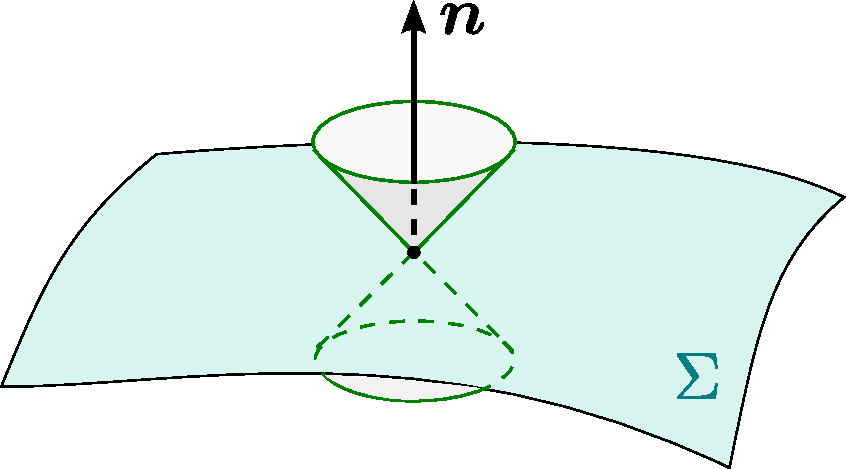
\includegraphics[width=0.45\textwidth]{def_spacelike_hyp.pdf}
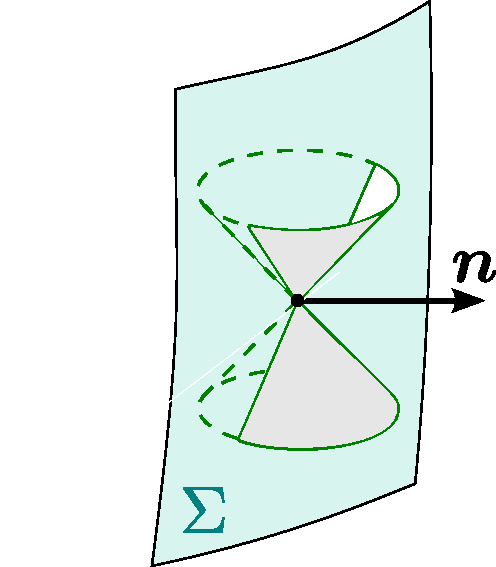
\includegraphics[width=0.25\textwidth]{def_timelike_hyp.pdf}
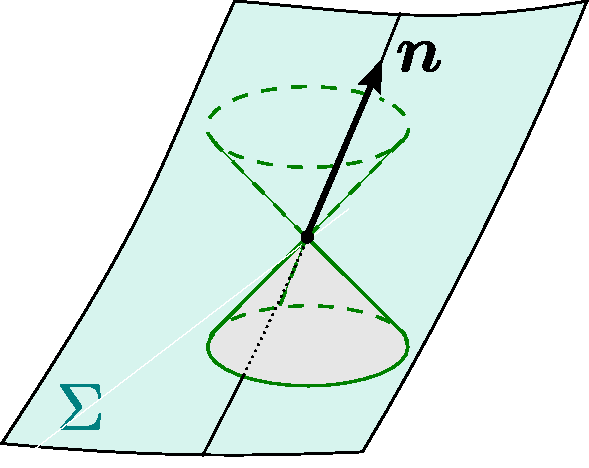
\includegraphics[width=0.30\textwidth]{def_null_hyp.pdf}}
\caption[]{\label{f:def:hypersurfaces} \footnotesize
The three types of hypersurfaces:
spacelike (left), timelike (middle) and null (right).}
\end{figure}

\subsection{The event horizon as a null hypersurface} \label{s:def:hor_as_null}

To discuss further which hypersurface could act as a black hole boundary,
one should recall that, on a Lorentzian manifold $(\M,\w{g})$, there are
three classes of hypersurfaces. The classification
depends on the type of metric induced by $\w{g}$ on the
hypersurface, $\Sigma$ say, the
\defin{induced metric}\index{induced!metric}\index{metric!induced --} being
nothing but the restriction $\left.\w{g}\right| _{\Sigma}$ of $\w{g}$
to vector fields tangent to $\Sigma$.
A hypersurface $\Sigma$ is said to be
\begin{itemize}
\item \defin{spacelike} iff $\left.\w{g}\right| _{\Sigma}$ is positive definite,
i.e. iff $\mathrm{sign} \left.\w{g}\right| _{\Sigma} = (+,+,+)$,
i.e. iff $(\Sigma,  \left.\w{g}\right| _{\Sigma})$ is a Riemannian manifold;
\item \defin{timelike} iff $\left.\w{g}\right| _{\Sigma}$ is a Lorentzian metric,
i.e. iff $\mathrm{sign} \left.\w{g}\right| _{\Sigma} = (-,+,+)$,
i.e. iff $(\Sigma,  \left.\w{g}\right| _{\Sigma})$ is a Lorentzian manifold;
\item \defin{null} iff $\left.\w{g}\right| _{\Sigma}$ is degenerate\footnote{
Cf. Sec.~\ref{s:bas:metric} in Appendix~\ref{s:bas} for the definition of a
degenerate bilinear form; the degeneracy
implies that the bilinear form $\left.\w{g}\right| _{\Sigma}$ is not,
strictly speaking, a metric on $\Sigma$.}
i.e. iff $\mathrm{sign} \left.\w{g}\right| _{\Sigma} = (0,+,+)$.
\end{itemize}
The hypersurface type can also be deduced from any normal vector\footnote{
The definition of a vector normal to a hypersurface is recalled in Sec.~\ref{s:bas:hyp_normal} of Appendix~\ref{s:bas}.}
$\w{n}$ to it (cf. Fig.~\ref{f:def:hypersurfaces}):
\begin{itemize}
\item $\Sigma$ spacelike $\iff$ $\w{n}$ timelike;
\item $\Sigma$ timelike $\iff$ $\w{n}$ spacelike;
\item $\Sigma$ null $\iff$ $\w{n}$ null.
\end{itemize}
These equivalences are easily proved by considering a $\w{g}$-orthogonal basis
adapted to $\Sigma$.

\begin{remark}
Null hypersurfaces have the distinctive feature that their normals are
also tangent to them. Indeed, by definition, the normal $\w{n}$ is null iff
$\w{n}\cdot\w{n}=0$, which is nothing but the condition
for $\w{n}$ to be tangent to $\Sigma$.
\end{remark}

\begin{figure}
\centerline{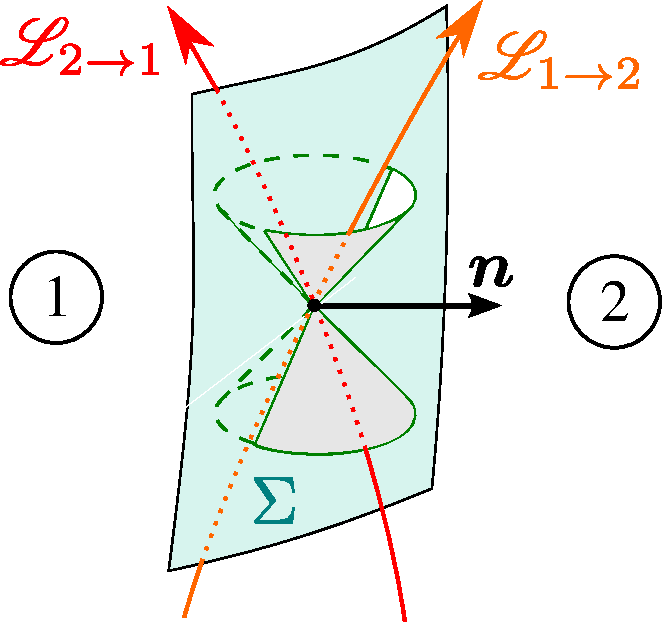
\includegraphics[width=0.4\textwidth]{def_timelike_2way.pdf}}
\caption[]{\label{f:def:timelike_2way} \footnotesize
A timelike hypersurface is a two-way membrane: $\Li_{1\rightarrow 2}$ is
a timelike worldline from Region~1 to Region~2, while $\Li_{2\rightarrow 1}$ is
a timelike worldline from Region~2 to Region~1.}
\end{figure}

\begin{figure}
\centerline{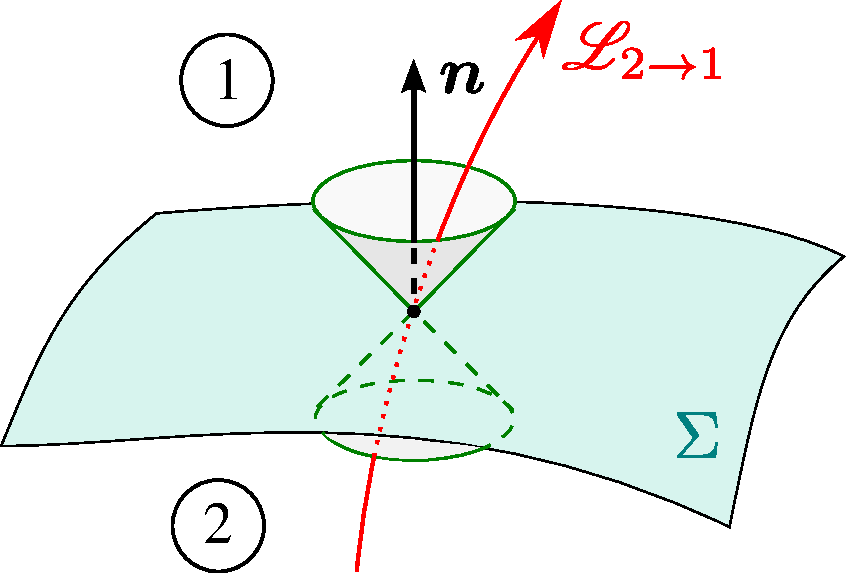
\includegraphics[width=0.5\textwidth]{def_spacelike_1way.pdf}}
\caption[]{\label{f:def:spacelike_1way} \footnotesize
A spacelike hypersurface is a one-way membrane: $\Li_{2\rightarrow 1}$ is
a timelike worldline from Region~2 to Region~1, while there is no timelike or null
worldline from Region~1 to Region~2.}
\end{figure}

\begin{figure}
\centerline{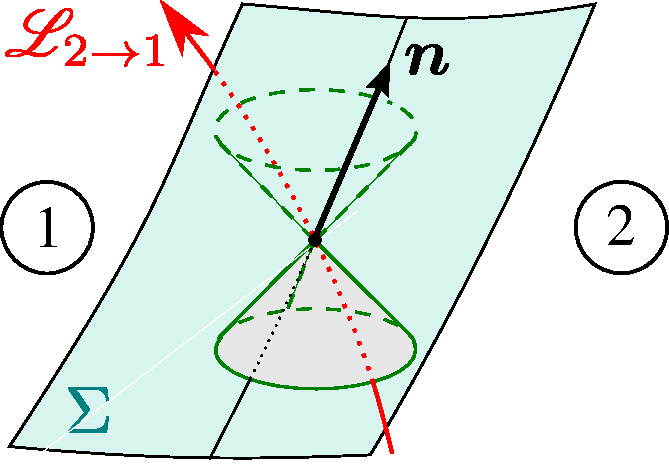
\includegraphics[width=0.5\textwidth]{def_null_1way.pdf}}
\caption[]{\label{f:def:null_1way} \footnotesize
A null hypersurface is a one-way membrane:: $\Li_{2\rightarrow 1}$ is
a timelike worldline from Region~2 to Region~1, while there is no timelike or null
worldline from Region~1 to Region~2.}
\end{figure}

A timelike hypersurface is a two-way membrane: if it divides (locally)
spacetime in two regions, 1 and 2 say, and a future-directed timelike or null
worldline can cross it from Region~1 to Region~2, or from Region~2 to Region~1
(see Fig.~\ref{f:def:timelike_2way}). On the contrary,
a spacelike hypersurface is a one-way membrane: a future-directed timelike or null
worldline, which is constrained to move inside the light cones,
can cross it only from Region~2 to Region~1, say (see Fig.~\ref{f:def:spacelike_1way}).
A null hypersurface is also a one-way membrane (see Fig.~\ref{f:def:null_1way}).
At most, a null worldline that is not going from Region~2 to Region~1 must
stay on the hypersurface; an exemple of such null wordline is
the one depicted in Fig.~\ref{f:def:null_1way} as the thin black line tangent to the normal $\w{n}$.

The limit case between two-way membranes (timelike hypersurfaces)
and one-way ones being null hypersurfaces, it is quite natural to select the
latter ones for the black hole boundary, rather than spacelike hypersurfaces.
This choice will be fully justified in Chap.~\ref{s:glo}, where we shall see
that the precise definition of a black hole implies that its boundary
(the event horizon\index{event!horizon}\index{horizon!event --})
is a null hypersurface as soon as it is smooth (Property~4 in Sec.~\ref{s:glo:properties_H}).
Note however that in Chap.~\ref{s:loc}, we shall see that spacelike hypersurfaces,
called \emph{dynamical
horizons}\index{dynamical!horizon}\index{horizon!dynamical --}, are involved
in quasi-local approaches to black holes.

%%%%%%%%%%%%%%%%%%%%%%%%%%%%%%%%%%%%%%%%%%%%%%%%%%%%%%%%%%%%%%%%%%%%%%%%%%%%%%%%

\section{Geometry of null hypersurfaces} \label{s:def:geom_null_hypsurf}

Having decided that the black hole event horizon must be a null hypersurface,
let us examine the geometrical properties of such hypersurfaces. We shall
denote the hypersurface under study by $\Hor$, for \emph{horizon}, but the results of this section
will be valid for any null hypersurface.

\subsection{Hypersurfaces as level sets}

As any hypersurface, $\Hor$ can be locally considered as a level set\index{level set}:
around any point of $\Hor$, there exists an open subset $\mathscr{U}$
of $\M$ (possibly  $\mathscr{U} = \M$) and
a smooth scalar field $u:\ \mathscr{U} \rightarrow \R$ such that
\be \label{e:def:Hor_u_zero}
    \forall p \in \mathscr{U},\quad p\in \Hor \iff u(p) = 0 .
\ee
and
\be \label{e:def:du_not_zero}
    \wnab u \not = 0 \quad \mbox{on}\ \Hor .
\ee
Condition (\ref{e:def:du_not_zero}) ensures that $\Hor$ is a regular
hypersurface (an \emph{embedded} submanifold, in mathematical terms); without it, $\Hor$ may have
self-intersection points.

\begin{figure}
\centerline{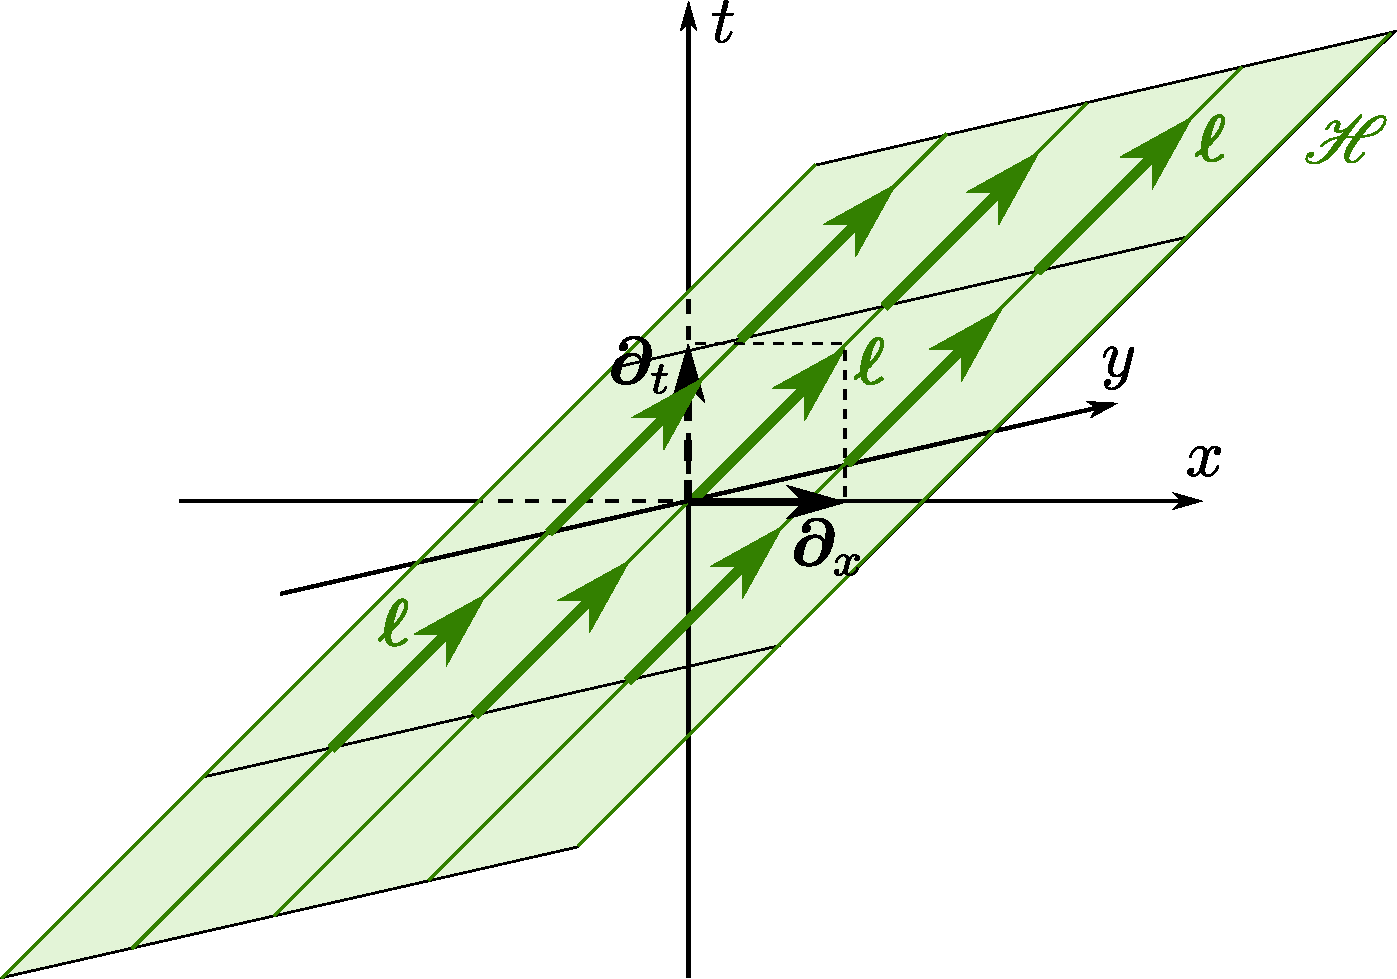
\includegraphics[width=0.6\textwidth]{def_null_hplane.pdf}}
\caption[]{\label{f:def:null_hplane} \footnotesize
Null hyperplane $\Hor$ of equation $t-x=0$ in Minkowski spacetime.
The dimension along $z$ has been suppressed, so that $\Hor$ is pictured as a
2-plane.}
\end{figure}


\begin{example}[null hyperplane] \label{x:def:null_hyp}
A very simple example of null hypersurface is a null hyperplane of
the 4-dimensional Minkowski spacetime. If $(t,x,y,z)$ are standard Minkowskian
coordinates, the choice of the scalar field
\be \label{e:def:null_plane_u}
    u(t,x,y,z) = t - x
\ee
defines a null hyperplane $\Hor$ by $u=0$ (cf. Fig.~\ref{f:def:null_hplane}).
\end{example}

\begin{example}[light cone] \label{x:def:light_cone}
Another simple example of null hypersurface, still in the 4-dimensional Minkowski spacetime,
is the future sheet $\Hor$ of a light cone\index{light!cone}\index{cone!light --}, also
called \defin{future light cone}\index{future!light cone}. Note that we have
to take out the cone apex from $\Hor$, in order to have a regular hypersurface.
In the  Minkowskian coordinates $(t,x,y,z)$, the choice of the
``retarded time''\index{retarded!time}
\be \label{e:def:light_cone_u}
    u(t,x,y,z) = t - \sqrt{x^2+y^2+z^2}
\ee
defines a future light cone $\Hor$ by $u=0$ and $t>0$ (cf.
Fig.~\ref{f:def:future_light_cone}).
\end{example}

\begin{figure}
\centerline{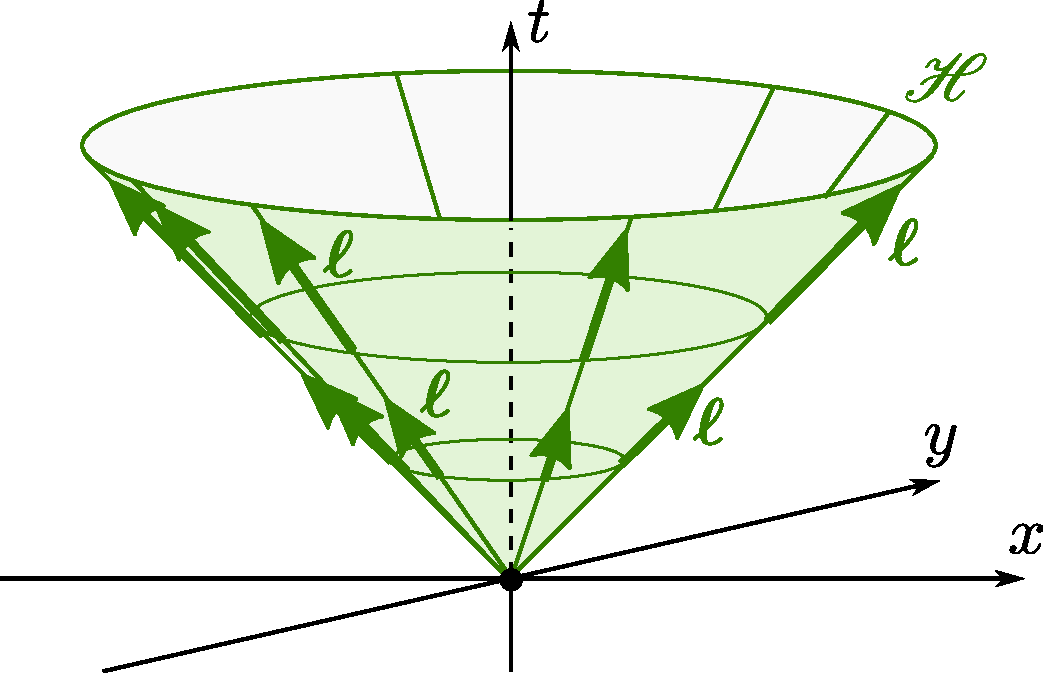
\includegraphics[width=0.6\textwidth]{def_future_light_cone.pdf}}
\caption[]{\label{f:def:future_light_cone} \footnotesize
Future sheet $\Hor$ of the light cone of equation $t-\sqrt{x^2+y^2+z^2}=0$ in Minkowski spacetime.
The dimension along $z$ has been suppressed, so that $\Hor$ looks 2-dimensional,
whereas it is actually 3-dimensional.}
\end{figure}


\begin{example}[Schwarzschild horizon] \label{x:def:Schw_hor}
Let us consider the 4-dimensional spacetime $(\M,\w{g})$ with $\M$ diffeomorphic
to $\mathbb{R}^4$ and equipped with a coordinate system $(x^\alpha)=(t,r,\th,\ph)$
($t\in \mathbb{R}$, $r\in(0,+\infty)$, $\th\in(0,\pi)$
and $\ph\in(0,2\pi)$) such that $\w{g}$ takes the form
\be \label{e:def:Schw_metric}
    g_{\mu\nu} \D x^\mu \D x^\nu = - \left( 1 - \frac{2 m}{r} \right) \D t^2
        + \frac{4m}{r} \, \D t \, \D r
        + \left( 1 + \frac{2 m}{r} \right) \D r^2
        + r^2\D\th^2 + r^2\sin^2\th \, \D\ph^2 ,
\ee
where $m$ is a positive constant. We shall see in Chap.~\ref{s:sch} that
$(\M,\w{g})$ is actually a part of Schwarzschild spacetime, described in
coordinates different from the standard Schwarzschild-Droste ones,  $(\bar t, r, \th, \ph)$
say, by the choice of the time coordinate:
$t = {\bar t} + 2m\ln|r/(2m)-1|$. The present coordinates are called
\defin{3+1 Eddington-Finkelstein coordinates}\index{Eddington-Finkelstein!coordinates}
and have the advantage over the the standard ones to be regular on the event horizon,
which is located at $r=2m$. Indeed, the metric components (\ref{e:def:Schw_metric})
remain finite when $r\rightarrow 2m$, as those of the inverse metric, which are
\be \label{e:def:Schw_metric_inv}
    g^{\alpha\beta} = \left(
    \begin{array}{cccc}
    - 1 - \frac{2m}{r} & \frac{2m}{r} & 0 & 0 \\
    \frac{2m}{r} & 1 - \frac{2m}{r} & 0 & 0 \\
    0 & 0 & \frac{1}{r^2} & 0 \\
    0 & 0 & 0 & \frac{1}{r^2\sin^2\th}
    \end{array} \right) .
\ee
Let us consider the scalar field defined on $\M$ by
\be \label{e:def:Schw_u}
    u(t,r,\th,\ph) = \left( 1 - \frac{r}{2m} \right)
            \exp\left(\frac{r-t}{4m}\right) .
\ee
It is then clear that the hypersurface $u=0$ is the
3-dimensional ``cylinder'' $\Hor$ of equation
$r=2m$ (cf. Fig.~\ref{f:def:Schwarz_horizon}). We shall see below\footnote{This should be obvious to the experienced
reader, since a normal 1-form to $\Hor$ is $\dd r$ and, from Eq.~(\ref{e:def:Schw_metric_inv}), $g^{rr}=0$ on $\Hor$.} that $\Hor$ is indeed a null hypersurface.
\end{example}

\begin{figure}
\centerline{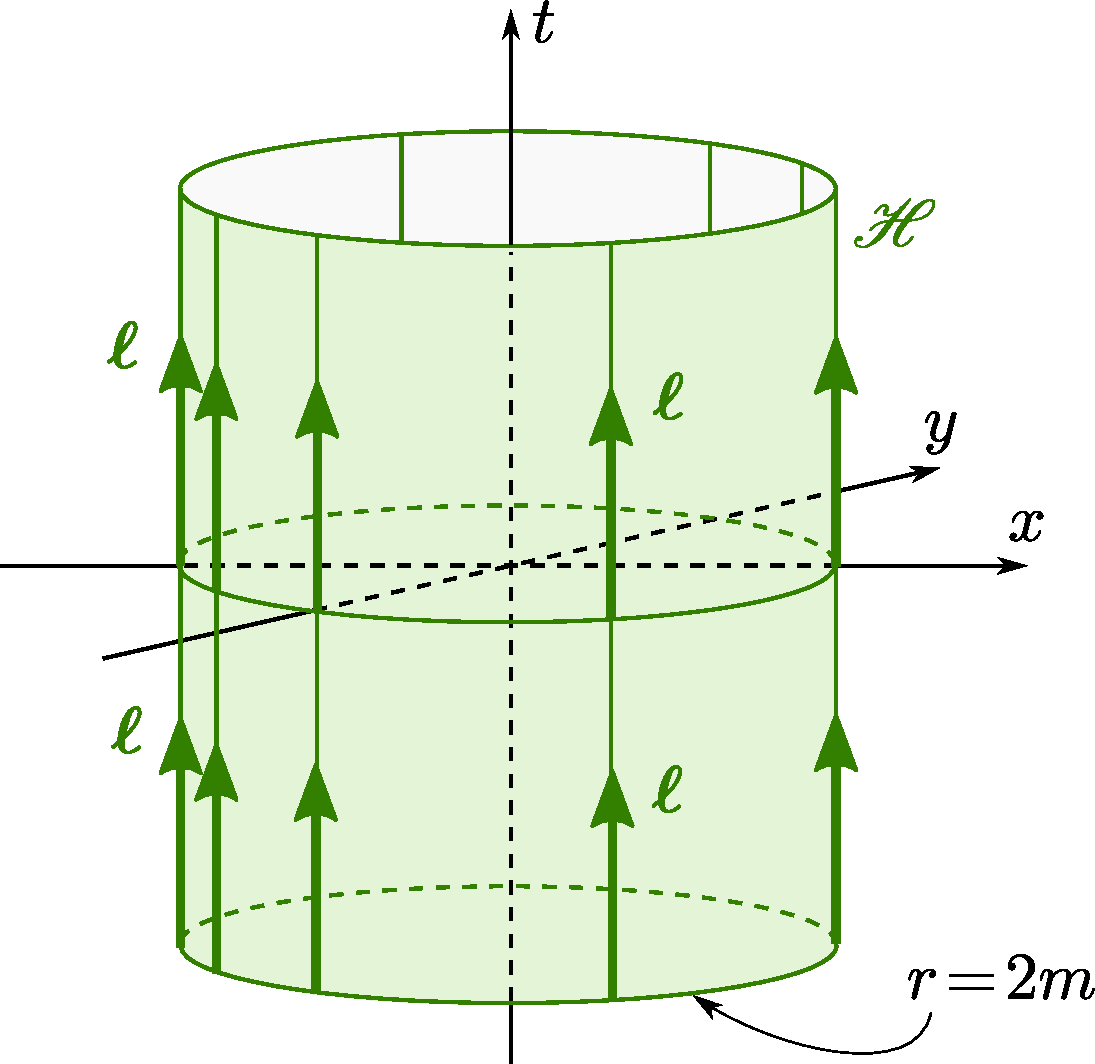
\includegraphics[width=0.5\textwidth]{def_Schwarz_horizon.pdf}}
\caption[]{\label{f:def:Schwarz_horizon} \footnotesize
Schwarzschild horizon $\Hor$ introduced in Example~\ref{x:def:Schw_hor};
The figure is drawn for $\th=\pi/2$ and is based on coordinates $(t,x,y)$
related to the 3+1 Eddington-Finkelstein coordinates $(t,r,\th,\ph)$
by $x=r\cos\ph$ and $y=r\sin\ph$.}
\end{figure}



\subsection{Null normals} \label{s:def:null_normal}

Let $\wl$ be a vector field normal to $\Hor$. Since $\Hor$ is a null hypersurface,
$\wl$ is a null vector:
\be \label{e:def:wl_null}
    \wl\cdot\wl = 0 .
\ee
Moreover, we choose $\wl$ to be future-directed (cf. Sec.~\ref{s:fra:spacetime}).

\begin{remark}
As a consequence of (\ref{e:def:wl_null}), there is no natural normalization
of $\wl$, contrary to the case of timelike or spacelike hypersurfaces,
where one can always choose the normal to be a unit vector
(scalar square equal to $1$ or $-1$). It follows that there is no unique choice
of $\wl$. At this stage, any rescaling $\wl \mapsto \wl' =  \alpha \wl$, with
$\alpha$ some strictly positive (to preserve the future orientation of $\wl$)
scalar field on $\Hor$,
yields a normal vector field $\wl'$ as valid as $\wl$.
\end{remark}
The null normal vector field $\wl$ is a priori defined on $\Hor$
only and not at points $p\not\in\Hor$.
However, it is worth to consider $\wl$ as a vector field
not confined to $\Hor$ but defined
in some open subset of $\M$ around $\Hor$.
In particular this would permit to define the spacetime covariant
derivative $\w{\nabla}\wl$, which is not possible if the
support of $\wl$ is restricted to $\Hor$.
Following Carter \cite{Carte97}, a simple way to achieve
this is to consider not only a single null hypersurface $\Hor$,
but a foliation of $\M$ (in the vicinity
of $\Hor$) by a family of null hypersurfaces, such that $\Hor$ is an
element of this family.
Without any loss of generality,
we may select the value of the scalar field $u$ defining $\Hor$ to label these hypersurfaces and
denote the family by $(\Hor_u)$. The null hypersurface $\Hor$
is then nothing but the element $\Hor = \Hor_{u=0}$ of this family
[Eq.~(\ref{e:def:Hor_u_zero})].
The vector field $\wl$ can then be viewed as being defined in the part of $\M$
foliated by $(\Hor_u)$, such that at each point in this region, $\wl$
is null and normal to $\Hor_u$ for some value of $u$.

\begin{example}
The scalar field $u$ introduced in Example~\ref{x:def:null_hyp}
(null hyperplane) does define a family of null hypersurfaces
$(\Hor_u)$. A counter-example would be $u(t,x,y,z)=(t-x)(1+x^2)$, since
$u=a$ does not define a null hypersurface except for $a=0$.
Similarly, the scalar fields $u$ of
Example~\ref{x:def:light_cone} (light cone)
and Example~\ref{x:def:Schw_hor} (Schwarzschild horizon)
do define a family of null
hypersurfaces $(\Hor_u)$. In the latter example, this would not have been the
case for the simpler choice $u(t,r,\th,\ph)  = r - 2m$.
\end{example}

Obviously the family $(\Hor_u)$ is non-unique but all geometrical
quantities that we shall introduce hereafter do not depend upon the choice
of the foliation $\Hor_u$ once they are evaluated at $\Hor$.

Since $\Hor$ is a hypersurface where $u$ is constant [Eq.~(\ref{e:def:Hor_u_zero})],
we have, by definition,
\bea
    \forall \w{v}\in T_p\M,\quad \w{v} \mbox{\ tangent to\ }\Hor & \iff  &
    \wnab_{\w{v}}\,  u = 0 \nonumber \\
    & \iff  & \langle \wnab u , \w{v} \rangle = 0 \nonumber \\
    & \iff & \vw{\nabla} u \cdot \w{v} = 0 ,   \label{e:def:nab_u_normal}
\eea
where $\vw{\nabla} u$ is the gradient vector field of the scalar field $u$,
i.e. the vector field given in index-notation by
\be \label{e:def:nab_up_u}
    \nabla^\alpha u = g^{\alpha\mu} \nabla_{\mu} u = g^{\alpha\mu} \der{u}{x^\mu} .
\ee
Property (\ref{e:def:nab_u_normal}) means that $\vw{\nabla} u$ is
a normal vector field to $\Hor$. By uniqueness of the normal direction to a hypersurface, it
must then be collinear to $\wl$. Therefore, there must exist some scalar
field $\rho$ such that
\be \label{e:def:wl_rho_u}
    \encadre{\wl = - e^\rho \, \vw{\nabla} u } .
\ee
We have chosen the
coefficient linking $\wl$ and $\vw{\nabla} u $ to be strictly negative,
i.e. under the form of minus an exponential. This is always possible by a suitable
choice of the scalar field $u$. The minus sign ensures that in the case
of $u$ increasing toward the future, $\wl$ is future-directed,
as the following example shows:

\begin{example}[null hyperplane] \label{x:def:null_hyp2}
We deduce from the
expression (\ref{e:def:null_plane_u}) chosen for $u$ in Example~\ref{x:def:null_hyp} that
\[
    \wnab u = \dd t - \dd x .
\]
The gradient vector field obtained by metric duality is
$\vw{\nabla} u = - \wpar_t - \wpar_x$. Choosing for simplicity $\rho=0$,
we get from formula~(\ref{e:def:wl_rho_u})
\be \label{e:def:wl_null_hyperplane}
    \wl =  \wpar_t + \wpar_x .
\ee
The vector field $\wl$ is depicted in Fig.~\ref{f:def:null_hplane}.
\end{example}

\begin{example}[light cone] \label{x:def:light_cone2}
Regarding Example~\ref{x:def:light_cone}, we have,
given expression (\ref{e:def:light_cone_u}) for $u$,
\[
    \wnab u = \dd t - \frac{x}{r} \dd x - \frac{y}{r} \dd y - \frac{z}{r} \dd z,
    \quad\mbox{with}\quad r:=\sqrt{x^2+y^2+z^2}.
\]
Choosing for simplicity $\rho=0$ in (\ref{e:def:wl_rho_u}), we get the
normal
\be \label{e:def:wl_light_cone}
    \wl = \wpar_t + \frac{x}{r} \wpar_x + \frac{y}{r} \wpar_y + \frac{z}{r} \wpar_z .
\ee
The vector field $\wl$ is depicted in Fig.~\ref{f:def:future_light_cone}.
\end{example}

\begin{example}[Schwarzschild horizon] \label{x:def:Schw_hor2}
We deduce from the expression (\ref{e:def:Schw_u}) chosen for $u$ in
Example~\ref{x:def:Schw_hor} that
\[
    \wnab u = \frac{1}{4 m} \mathrm{e}^{(r-t)/(4m)} \left[ - \left(1-\frac{r}{2m}  \right)
        \, \dd t
        - \left(1 + \frac{r}{2m}\right) \, \dd r \right] .
\]
The corresponding gradient vector field,
is computed from (\ref{e:def:nab_up_u}) via expression
(\ref{e:def:Schw_metric_inv}) for $g^{\alpha\mu}$:
\[
    \vw{\nabla} u = \frac{1}{4 m} \mathrm{e}^{(r-t)/(4m)} \left[
    - \left(1+ \frac{r}{2m} \right) \wpar_t
    + \left(1 - \frac{r}{2m} \right) \wpar_r \right] .
\]
This time, we do not chose $\rho=0$ but rather select $\rho$ so that
$\el^t = 1$:
\be \label{e:def:rho_Schw_hor}
    e^\rho =  - \frac{1}{\nabla^t u} \iff
    \rho = \frac{t-r}{4m} - \ln \left( 1 + \frac{r}{2m} \right) + \ln (4 m).
\ee
Equation~(\ref{e:def:wl_rho_u}) leads then to
\be \label{e:def:wl_Schw_hor}
    \wl = \wpar_t +  \frac{r-2m}{r+2m} \,  \wpar_r .
\ee
Given the metric (\ref{e:def:Schw_metric}), we check that $\w{g}(\wl, \wl)=0$.
Since $\wl\not=0$, this proves that all hypersurfaces $\Hor_u$, and in particular $\Hor$,
are null.
The vector field $\wl$ is depicted in Fig.~\ref{f:def:Schwarz_horizon}.
\end{example}

\subsection{Null geodesic generators}

\subsubsection{Frobenius identity}

Let us take the metric dual of relation (\ref{e:def:wl_rho_u}): it writes
$\uu{\el} = - e^\rho \, \wnab u$, or, in index notation,
\be
    \el_\alpha = - e^\rho \, \nabla_\alpha u .
\ee
Taking the covariant derivative, we get
\[
    \nabla_\alpha \el_\beta = - e^\rho \nabla_\alpha \rho \nabla_\beta u
                -   e^\rho  \nabla_\alpha \nabla_\beta u
                 = \nabla_\alpha \rho \, \el_\beta - e^\rho  \nabla_\alpha \nabla_\beta u
\]
Antisymmetrizing and using the torsion-free property of $\wnab$ (i.e.
$\nabla_\alpha \nabla_\beta u - \nabla_\beta \nabla_\alpha u = 0$, cf.
Eq.~(\ref{e:bas:torsion-free}) in Appendix~\ref{s:bas}), we get
\be \label{e:def:ext_der_wl_comp}
  \nabla_\alpha \el_\beta - \nabla_\beta \el_\alpha =
  \nabla_\alpha \rho \, \el_\beta -  \nabla_\beta \rho \, \el_\alpha  .
\ee
In the left-hand side there appears the exterior derivative of
the 1-form $\uu{\el}$ (cf. Sec.~\ref{s:bas:ext_deriv} in Appendix~\ref{s:bas}),
while one recognize in the right-hand side the exterior product of
the two 1-forms $\dd\rho$ and $\uu{\el}$. Hence we may rewrite (\ref{e:def:ext_der_wl_comp})
as
\be
    \encadre{ \dd \uu{\el} = \dd\rho \wedge \uu{\el} } .
\ee
This reflects the \defin{Frobenius theorem}\index{Frobenius!theorem}
in its dual formulation (see e.g.
Theorem B.3.2 in Wald's textbook \cite{Wald84}): the exterior derivative of
the 1-form $\uu{\el}$ is the exterior product of $\uu{\el}$ itself with some
1-form ($\dd\rho$ in the present case) if, and only if,
$\uu{\el}$ defines hyperplanes that are integrable in some hypersurface ($\Hor$ in the present case).

\subsubsection{Geodesic generators} \label{s:def:geod_gener}

Let us contract the Frobenius identity (\ref{e:def:ext_der_wl_comp}) with $\wl$:
\be \label{e:def:l_contract_Frob}
    \el^\mu \nabla_\mu \el_\alpha - \el^\mu \nabla_\alpha \el_\mu
        = \el^\mu \nabla_\mu \rho \, \el_\alpha
        - \underbrace{\el^\mu \el_\mu}_{0} \nabla_\alpha \rho .
\ee
Now, since $\wl$ is a null vector,
\[
    \el^\mu \nabla_\alpha \el_\mu = \nabla_\alpha (\underbrace{\el^\mu \el_\mu}_{0})
        - \el_\mu \nabla_\alpha \el^\mu ,
\]
from which we get
\be \label{e:def:el_nab_el_zero}
    \el^\mu \nabla_\alpha \el_\mu = 0 .
\ee
Hence (\ref{e:def:l_contract_Frob}) reduces to
\be \label{e:def:wl_geod_kappa_dual}
    \el^\mu \nabla_\mu \el_\alpha  = \kappa \, \el_\alpha ,
\ee
with
\be \label{e:def:def_kappa}
    \kappa := \el^\mu \nabla_\mu \rho = \wnab_{\wl}\,  \rho .
\ee
The metric dual of (\ref{e:def:wl_geod_kappa_dual}) is
\be \label{e:def:wl_geod_kappa}
    \encadre{ \wnab_{\wl}\, \wl = \kappa \, \wl } .
\ee
This equation implies that the field lines of $\wl$ are geodesics.
To demonstrate this, we note that a rescaling
\be \label{e:def:wl_rescale}
    \wl \mapsto \wl' =  \alpha \wl
\ee
with $\alpha$ a strictly positive scalar field can be performed to yield
a \defin{geodesic vector field}\index{geodesic!vector field} $\wl'$, i.e.
a vector field that obeys\footnote{A vector field that obeys the weaker condition
(\ref{e:def:wl_geod_kappa}) with $\kappa$ possibly different from zero is called
a \defin{pregeodesic vector field}\index{pregeodesic vector field}, cf. Remark~\ref{r:fra:geodesic_vector}
on page~\pageref{r:fra:geodesic_vector}.}
\be \label{e:def:wlp_geod}
    \wnab_{\wl'}\, \wl' = 0 .
\ee
\begin{proof}
Equations~(\ref{e:def:wl_rescale}) and
(\ref{e:def:wl_geod_kappa}) imply
\be \label{e:def:nab_lp_lp}
    \wnab_{\wl'}\, \wl' = \alpha\left(
        \wnab_{\wl}\, \alpha + \kappa \alpha \right) \wl .
\ee
Hence, since $\alpha>0$,
\[
    \wnab_{\wl'}\, \wl' = 0  \iff  \wnab_{\wl}\, \ln \alpha = -\kappa .
\]
Therefore it suffices to solve $\wnab_{\wl}\, \ln \alpha = -\kappa$, which
is a first-order ordinary differential equation along each field line of $\wl$,
to ensure that $\wl'$ is a geodesic vector field.
\end{proof}
Because of (\ref{e:def:wlp_geod}),
the field lines of $\wl'$ are  null geodesics and $\wl'$ is the tangent
vector to them associated with some affine parameter $\lambda$.
On the other side, if $\kappa\not=0$, $\wl$ is not a geodesic vector field
and therefore cannot be associated with some affine parameter. For this
reason the quantity $\kappa$ is called the
\defin{non-affinity coefficient}\index{non-affinity coefficient} of
the null normal $\wl$.

Since $\wl$ is collinear to $\wl'$, it obviously shares the same field lines,
which have just been shown to be null geodesics. These field lines are called the
\defin{null geodesic generators}\index{null!geodesic!generator}\index{generator!of a null hypersurface} of the hypersurface $\Hor$.

Hence, we have shown that
\begin{greybox}
Any null hypersurface $\Hor$ is ruled by a family of null geodesics, called the
\emph{generators of $\Hor$}, and each vector field $\wl$ normal to $\Hor$ is
tangent to these null geodesics.
\end{greybox}

\begin{remark}
\label{r:def:null_curves}
The above result is not trivial: while it is obvious that the field lines of the normal
vector field $\wl$ are null curves that are tangent to $\Hor$, the reader must
keep in mind that not all null curves are null geodesics. For instance, in
Minkowski spacetime, the helix defined in terms of
some Minkowskian coordinates $(x^\alpha)=(t,x,y,z)$ by the parametric equation
$x^\alpha(\lambda) = (\lambda, \cos\lambda, \sin\lambda, 0)$ is a null curve, i.e.
it has
a null tangent vector at each point, but it is not a null geodesics (in Minkowski
spacetime, all null geodesics are straight lines).
\end{remark}

As a by-product of (\ref{e:def:nab_lp_lp}), we get the behaviour of the
non-affinity coefficient under a rescaling of the null normal:
\be \label{e:def:rescale_kappa}
    \wl' = \alpha \wl \ \Longrightarrow \ \kappa' = \alpha \kappa + \wnab_{\wl} \alpha .
\ee

\begin{example}[null hyperplane] \label{x:def:null_hyp3}
It is clear on expression (\ref{e:def:wl_null_hyperplane}) for $\wl$ that
the covariant derivative
$\wnab \wl$ vanishes identically. In particular $\wnab_{\wl} \wl = 0$.
Equation~(\ref{e:def:wl_geod_kappa}) then implies
\be \label{e:def:kappa_0_nullhyp}
    \kappa = 0 ,
\ee
which is in agreement with Eq.~(\ref{e:def:def_kappa}) and the choice $\rho=0$
performed in Example~\ref{x:def:null_hyp2}. The null geodesic generators of $\Hor$ are the
straight lines defined by $t=x$, $y=y_0$ and $z=z_0$ for some constants
$(y_0,z_0)\in \mathbb{R}^2$.
They are depicted as green lines in Fig.~\ref{f:def:null_hplane}.
 Either $t$ or $x$ can be chosen as affine
parameters of these generators.
\end{example}

\begin{example}[light cone] \label{x:def:light_cone3}
From expression (\ref{e:def:wl_light_cone})
for $\wl$ and the fact that
$\nabla_\beta \el^\alpha = \partial_\beta \el^\alpha$
in the Minkowskian coordinates $(t,x,y,z)$, we get
\be \label{e:def:nab_l_light_cone}
    \nabla_\beta \el^\alpha = \left(
    \begin{array}{cccc}
    0 & 0 & 0 & 0 \\
    0 & \frac{y^2+z^2}{r^3} & - \frac{xy}{r^3} & - \frac{xz}{r^3} \\
    0 & - \frac{xy}{r^3} & \frac{x^2+z^2}{r^3} & - \frac{yz}{r^3} \\
    0 & - \frac{xz}{r^3} & - \frac{yz}{r^3} & \frac{x^2+y^2}{r^3}
    \end{array} \right)
    \qquad {(\alpha = \mbox{row index}; \atop \beta = \mbox{column index}).}
\ee
We obtain then $\el^\mu \nabla_\mu \el^\alpha = 0$.
From Eq.~(\ref{e:def:wl_geod_kappa}), we conclude that
\[
    \kappa = 0 ,
\]
which is in agreement with Eq.~(\ref{e:def:def_kappa}) and the choice $\rho=0$
performed in Example~\ref{x:def:light_cone2}. The null geodesic generators of $\Hor$
are the half-lines defined by $x=a t$, $y=b t$, $z = \sqrt{1-a^2-b^2} t$, with
$t>0$ and $(a,b)\in\mathbb{R}^2$ such that $a^2+b^2 \leq 1$.
They are depicted as green lines in Fig.~\ref{f:def:future_light_cone}.
Since from (\ref{e:def:wl_light_cone}) $\wnab_{\wl} t = 1$
and $\kappa=0$, $\lambda=t$ is an affine parameter along these null geodesic generators.
\end{example}

\begin{example}[Schwarzschild horizon] \label{x:def:Schw_hor3}
The covariant derivative of the vector field $\wl$ as given by (\ref{e:def:wl_Schw_hor})
is (cf. Appendix~\ref{s:sam} for the computation)
\be \label{e:def:nab_l_Schw_hor}
    \nabla_\beta \el^\alpha = \left(
    \begin{array}{cccc}
    \frac{m}{r^2} & \frac{m}{r^2} \frac{3r+2m}{r+2m} & 0 & 0 \\[1ex]
    \frac{m}{r^2}\frac{r-2m}{r+2m} & \frac{m}{r^2}\frac{3r^2-4m(r+m)}{(r+2m)^2} & 0 & 0 \\[1ex]
    0 & 0 & \frac{r-2m}{r(r+2m)} & 0 \\
    0 & 0 & 0 & \frac{r-2m}{r(r+2m)}
    \end{array} \right)
    \qquad {(\alpha = \mbox{row index}; \atop \beta = \mbox{column index}).}
\ee
Contracting with $\wl^\beta$, we obtain
\[
    \wnab_{\wl} \wl = \frac{4m}{(r+2m)^2} \wpar_t
        +  \frac{4m(r-2m)}{(r+2m)^3} \,  \wpar_r = \frac{4m}{(r+2m)^2}  \, \wl .
\]
Hence, for any $\Hor_u$, $\kappa=4m/(r+2m)^2$. On $\Hor$ ($r=2m$), we get
\be \label{e:def:kappa_Schw_hor}
   \kappa = \frac{1}{4m} .
\ee
This value agrees with $\kappa = \wnab_{\wl}\rho$ [Eq.~(\ref{e:def:def_kappa})] and the
choice (\ref{e:def:rho_Schw_hor}) made for $\rho$. Contrary to Examples~\ref{x:def:null_hyp3}
and \ref{x:def:light_cone3}, $\kappa$ does not vanish; hence $t$, which is
a parameter of the null geodesic generators associated with $\wl$ (since $\wnab_{\wl} t = 1$
by virtue of (\ref{e:def:wl_Schw_hor})),
is \emph{not} an affine parameter. The null geodesic generators are depicted
as vertical green lines in Fig.~\ref{f:def:Schwarz_horizon}.
\end{example}

\subsection{Cross-sections} \label{s:def:spacelike_sections}

Let us now focus on the first aspect of the black hole definition given
in Sec.~\ref{s:def:first_defin}: \emph{localization}.
This feature is crucial to distinguish a black hole boundary from other types
of null hypersurfaces. For instance the interior of a future null cone
in Minkowski spacetime is a region from which no particle may escape,
but since the null cone is expanding, particles can travel arbitrary far from
the centre. Therefore a null cone does not define a black hole.
A key parameter is hence the \emph{expansion} of null hypersurfaces, which we shall
discuss in the next section, after having introduced cross-sections.

\begin{figure}
\vspace{5cm}
%\centerline{\includegraphics[width=0.6\textwidth]{}}
\caption[]{\label{f:def:hor_cylinder} \footnotesize
The null hypersurface $\Hor$ and some cross-sections.}
\end{figure}

In the remaining of this chapter, we assume that the spacetime dimension
obeys $n\geq 3$. We define then a \defin{cross-section}\index{cross-section}
of the null hypersurface $\Hor$
as a submanifold $\Sp$ of $\Hor$ of codimension 2 (i.e. $\dim \Sp=n-2$),
such that (i) the null normal $\wl$ is nowhere tangent to $\Sp$ and (ii)
each null geodesic generator of $\Hor$ intersects $\Sp$ once, and only once.

\begin{notation}
Indices relative to a cross-section will range from $2$ to $n-1$ and
will be denoted by a Latin letter from the beginning of the alphabet: $a$, $b$, etc.
\end{notation}

To encompass the idea that an event horizon delimitates some
region of spacetime, we shall assume that the cross-sections
are \defin{closed manifolds}\index{closed!manifold}, i.e.
are compact without boundary. The simplest example is the sphere,
more precisely the $(n-2)$-dimensional sphere $\mathbb{S}^{n-2}$, where $n$
is the spacetime dimension. It is the one relevant for standard 4-dimensional
black holes. But at this stage, we shall allow for other
closed-manifold topologies, like that of a torus.

Given the definition of a cross-section $\Sp$,
the topology of $\Hor$ is then that of a ``tube'' or ``cylinder''
(cf. Fig.~\ref{f:def:hor_cylinder}):
\be \label{e:def:H_topology}
    \Hor \simeq \R \times \Sp.
\ee
For the standard 4-dimensional black holes, this is
$\Hor \simeq \R \times \mathbb{S}^{2}$.

A first important property of any cross-section $\Sp$ is to be spacelike,
i.e. every vector
tangent to $\Sp$ must be spacelike.
\begin{proof}
The spacelike character of $\Sp$ follows from the following
lemma\footnote{\emph{Exercise:} prove it!}:
\begin{greybox}
Every nonzero vector tangent to a null hypersurface is either spacelike or null.
Moreover, in the latter case, it is tangent to a null geodesic generator (i.e. it is normal
to the hypersurface).
\end{greybox}
Let $p \in \Sp$ and $\w{v}\in T_p\M$ be a nonzero vector tangent to $\Sp$.
The above lemma implies that $\w{v}$ is either spacelike or tangent to the
null geodesic generator $\Li$ going through $p$, but then $\Li$ would be tangent to $\Sp$,
which is not allowed, given the definition of a cross-section. We conclude
that $\w{v}$ is necessarily spacelike, which proves that $\Sp$ is a spacelike
submanifold.
\end{proof}

\begin{example}[light cone] \label{x:def:light_cone4}
From now on, we abandon the null hyperplane considered in Examples~\ref{x:def:null_hyp},
\ref{x:def:null_hyp2} and \ref{x:def:null_hyp3}, since its topology is $\mathbb{R}^3$,
and therefore not of the type (\ref{e:def:H_topology}) with $\Sp$ compact.
On the other side, the future sheet $\Hor$ of the light cone of Minkowski spacetime considered in Examples~\ref{x:def:light_cone},
\ref{x:def:light_cone2} and \ref{x:def:light_cone3} does obey (\ref{e:def:H_topology}),
since we have excluded the cone apex from $\Hor$.
A natural choice of cross-section is a sphere defined by $t=t_0$ for some positive constant $t_0$:
\[
    \Sp = \left\{ p \in \Hor,\  t(p) = t_0 \right\} .
\]
That $\Sp$ is a 2-dimensional sphere in the hyperplane $t=t_0$ is clear on its equation in terms
of the Minkowskian coordinates $(t,x,y,z)$:
\[
\Sp: \quad t=t_0 \quad\mbox{and}\quad x^2+y^2+z^2 = t_0^2,
\]
which follows immediately from $u=0$
[cf. Eq.~(\ref{e:def:light_cone_u})]. Moreover, this equation shows that the
radius of the sphere is $t_0$.
\end{example}

\begin{example}[Schwarzschild horizon] \label{x:def:Schw_hor4}
The 3-dimensional cylinder $\Hor$ introduced in Example~\ref{x:def:Schw_hor}
has the topology (\ref{e:def:H_topology}), with $\Sp\simeq \mathbb{S}^2$
(cf. Fig.~\ref{f:def:Schwarz_horizon}).
Since it is defined
by $r=2m$ in terms of the 3+1 Eddington-Finkelstein coordinates $(t,r,\th,\ph)$,
a natural coordinate system on $\Hor$ is $x^A = (t,\th,\ph)$. Moreover, we
have seen that the coordinate $t$ is the (non-affine) parameter of the null
geodesics generating $\Hor$ associated with the null normal $\wl$.
As in Example~\ref{x:def:light_cone4}, a natural choice of cross-section is a
sphere defined by $t=t_0$ for some constant $t_0$:
\[
    \Sp = \left\{ p \in \Hor,\  t(p) = t_0 \right\} .
\]
The equation of $\Sp$ in terms of the coordinates $(t,r,\th,\ph)$ is then
\[
    \Sp: \quad t=t_0 \quad\mbox{and}\quad r = 2m .
\]
Note that $x^a=(\th,\ph)$ constitutes a coordinate system on $\Sp$.
\end{example}

\begin{example}[binary black hole]
Some cross-sections of the event horizon $\Hor$ in numerically
generated binary black hole spacetimes are displayed in Figs.~\ref{f:glo:EH_headon}
and \ref{f:glo:EH_binspir} of Chap.~\ref{s:glo}.
\end{example}

Let us denote by $\w{q}$ the
\defin{metric induced on $\Sp$ by $\w{g}$}\index{induced!metric}\index{metric!induced --},
i.e. the bilinear form defined at any point $p\in\Sp$ by
\be \label{e:def:def_q_S}
    \forall (\w{u},\w{v})\in T_p\Sp\times T_p\Sp, \quad
     \w{q}(\w{u},\w{v}) = \w{g}(\w{u},\w{v}) .
\ee
Saying that $\Sp$ is spacelike is equivalent to saying that $\w{q}$ is
positive definite, i.e.
\be
    \forall \w{v}\in T_p\Sp,\quad
    \w{q}(\w{v},\w{v}) \geq 0 \quad \mbox{and} \quad
    \w{q}(\w{v},\w{v}) = 0 \iff \w{v} = 0.
\ee
In other words, $(\Sp, \w{q})$ is a \defin{Riemannian manifold}\index{Riemannian!manifold} (cf Sec.~\ref{s:bas:signature} in Appendix~\ref{s:bas}).

\begin{example}[Schwarzschild horizon] \label{x:def:Schw_hor4a}
The metric induced by $\w{g}$ on the cross-section
$\Sp$ of the Schwarzschild horizon defined in Example~\ref{x:def:Schw_hor4} is readily obtained by
setting $t=\mathrm{const}=t_0$ and $r=\mathrm{const}=2m$ in Eq.~(\ref{e:def:Schw_metric}),
since  $x^a=(\th,\ph)$ is a coordinate system on $\Sp$:
\be \label{e:def:q_S_Schw_hor}
    q_{ab} \D x^a \D x^b = 4m^2 \left( \D\th^2 + \sin^2\th \D^2\ph \right) .
\ee
\end{example}

\begin{figure}
\vspace{5cm}
%\centerline{\includegraphics[width=0.6\textwidth]{}}
\caption[]{\label{f:def:TS_ortho} \footnotesize
The tangent space to the cross-section $\Sp$ and its orthogonal complement.}
\end{figure}

An important consequence of $\Sp$ being spacelike is that, at each point
$p\in \Sp$, the tangent space $T_p\Sp$ has an orthogonal complement
$T_p^\perp\Sp$,  which is a timelike plane such that
$T_p\M$ is the direct sum of $T_p\Sp$ and $T_p^\perp\Sp$ :
\be \label{e:def:TM_direct_sum}
   \encadre{ \forall p\in \Sp,\quad T_p\M = T_p\Sp \oplus T_p^\perp\Sp }.
\ee
That $T_p^\perp\Sp$ is timelike is necessary for the signature of $\w{g}$
to be $(-,+,\ldots,+)$. This can be seen by constructing an $\w{g}$-orthogonal
basis of $T_p\M$ by the Gram-Schmidt process, starting form a
$\w{q}$-orthogonal basis of $T_p\Sp$. Since $\dim T_p\Sp = n-2$, we have
$\dim T_p^\perp\Sp = 2$, i.e. $T_p^\perp\Sp$ is a timelike 2-plane.
In other words, the metric induced by $\w{g}$ on
$T_p^\perp\Sp$ is Lorentzian:
\be
    \mathrm{sign}\, \left.\w{g}\right|_{T_p^\perp\Sp} = (-,+) .
\ee
By definition, the null normal $\wl$ is orthogonal to any vector
tangent to $\Sp$, i.e. $\wl \in T_p^\perp\Sp$.
Since $T_p^\perp\Sp$ is a timelike plane, it has two independent null directions,
which can be seen as the two intersections of the null cone at $p$ with
the 2-plane $T_p^\perp\Sp$ (cf. Fig.~\ref{f:def:TS_ortho}).
Let us denote by $\w{k}$ a future-directed null vector in the null direction of $T_p^\perp\Sp$
that is not along $\wl$. By a proper rescaling $\w{k}\mapsto \alpha\w{k}$,
we may choose $\w{k}$ so that
\be \label{e:def:k_el_minus_one}
        \w{k}\cdot\wl = -1 .
\ee
Given $\wl$ and $\Sp$, the condition (\ref{e:def:k_el_minus_one})
determines the null vector $\w{k}$ uniquely.
Since $\wl$ and $\w{k}$ are non-collinear vectors of $T_p^\perp\Sp$ and
$\dim T_p^\perp\Sp = 2$, they constitute a basis of $T_p^\perp\Sp$:
\be \label{e:def:TSperp_Span_k_l}
    T_p^\perp\Sp = \mathrm{Span}\left( \wl, \w{k} \right) .
\ee

A priori, the bilinear form $\w{q}$ is defined only on $T_p\Sp$, via (\ref{e:def:def_q_S}).
However, thanks to the orthogonal decomposition (\ref{e:def:TM_direct_sum}),
we can extend it to all vectors of $T_p\M$ by requiring
\be \label{e:def:q_zero_TSperp}
    \forall \w{v}\in T_p^\perp\Sp, \quad \w{q}(\w{v}, .) = 0 .
\ee
Indeed, given a pair $(\w{u},\w{v})$ of vectors in $T_p\M$, (\ref{e:def:TM_direct_sum})
implies that there are unique decompositions
\bea
  & & \w{u} = \w{u}^\parallel + \w{u}^\perp,\quad \mbox{with}\quad  \w{u}^\parallel \in T_p\Sp,
    \  \w{u}^\perp \in T_p^\perp\Sp \label{e:def:decomp_u} \\
  & & \w{v} = \w{v}^\parallel + \w{v}^\perp,\quad \mbox{with}\quad  \w{v}^\parallel \in T_p\Sp,
    \  \w{v}^\perp \in T_p^\perp\Sp .\label{e:def:decomp_v}
\eea
Then, using the bilinearity of $\w{q}$ and the property (\ref{e:def:q_zero_TSperp}),
we obtain
\be \label{e:def:q_all_vectors}
    \forall (\w{u},\w{v})\in T_p\M\times T_p\M, \quad
     \w{q}(\w{u},\w{v}) = \w{q}(\w{u}^\parallel,\w{v}^\parallel) .
\ee
Equation~(\ref{e:def:q_all_vectors}), along with (\ref{e:def:def_q_S}), can
be considered as the definition of $\w{q}$. An equivalent definition,
which provides an explicit expression of $\w{q}$, is
\be \label{e:def:q_g_k_l}
    \encadre{ \w{q} = \w{g} + \uu{\el}\otimes\uu{k} + \uu{k}\otimes\uu{\el} } ,
\ee
or, in index notation,
\[
    q_{\alpha\beta} = g_{\alpha\beta} + \el_\alpha k_\beta + k_\alpha \el_\beta .
\]
\begin{proof}
Let us show that (\ref{e:def:q_g_k_l}) implies
(\ref{e:def:q_all_vectors})-(\ref{e:def:def_q_S}).
Starting from (\ref{e:def:q_g_k_l}), we have for any pair of vectors $(\w{u},\w{v})$
in $T_p\M$,
\be \label{e:def:q_u_v_k_l}
    \w{q}(\w{u},\w{v}) = \w{u}\cdot\w{v} + (\wl\cdot\w{u})(\w{k}\cdot\w{v})
    + (\w{k}\cdot\w{u})(\wl\cdot\w{v}) .
\ee
Now, thanks to (\ref{e:def:TSperp_Span_k_l}), we may write the
orthogonal decompositions
(\ref{e:def:decomp_u})-(\ref{e:def:decomp_v}) as
\[
    \w{u} = \w{u}^\parallel + u^0 \wl + u^1 \w{k} \quad\mbox{and}\quad
    \w{v} = \w{v}^\parallel + v^0 \wl + v^1 \w{k} .
\]
Using $\wl\cdot\wl=0$, $\w{k}\cdot\w{k}=0$ and $\wl\cdot\w{k}=-1$
[Eq.~(\ref{e:def:k_el_minus_one})], we have then
\bea
 & & \w{u}\cdot\w{v} = \w{u}^\parallel \cdot\w{v}^\parallel - u^0 v^1 - u^1 v^0 \nonumber \\
 & & \wl\cdot\w{u} = -u^1, \quad \w{k}\cdot\w{u} = -u^0, \nonumber \\
 & & \wl\cdot\w{v} = -v^1, \quad \w{k}\cdot\w{v} = -v^0 .  \nonumber
\eea
Hence (\ref{e:def:q_u_v_k_l}) results in
\bea
    \w{q}(\w{u},\w{v}) & = & \w{u}^\parallel \cdot\w{v}^\parallel - u^0 v^1 - u^1 v^0
            + u^1 v^0 + u^0 v^1 \nonumber \\
                & = & \w{u}^\parallel \cdot\w{v}^\parallel,  \nonumber
\eea
which is nothing but (\ref{e:def:q_all_vectors}).
\end{proof}

\begin{example}[light cone] \label{x:def:light_cone5}
In continuation with Example~\ref{x:def:light_cone4}, the null
vector $\w{k}$ orthogonal to the sphere $\Sp$ and obeying $\w{k}\cdot\wl = -1$
is
\[
    \w{k} = \frac{1}{2} \wpar_t
        - \frac{x}{2r} \wpar_x - \frac{y}{2r} \wpar_y  - \frac{z}{2r} \wpar_z .
\]
Evaluating $\w{q}$ via (\ref{e:def:q_g_k_l}), given expression
(\ref{e:def:wl_light_cone}) for $\wl$, we get the following components
of $\w{q}$ with respect to the Minkowskian coordinates $x^\alpha=(t,x,y,z)$:
\[
    q_{\alpha\beta} = \left(
    \begin{array}{cccc}
    0 & 0 & 0 & 0 \\
    0 & \frac{y^2+z^2}{r^2} & - \frac{xy}{r^2} & - \frac{xz}{r^2} \\
    0 & - \frac{xy}{r^2} & \frac{x^2+z^2}{r^2} & - \frac{yz}{r^2} \\
    0 & - \frac{xz}{r^2} & - \frac{yz}{r^2} & \frac{x^2+y^2}{r^2}
    \end{array} \right) .
 \]
If we consider the spherical coordinates ${x'}^{\alpha}=(t,r,\th,\ph)$
deduced from the Minkowskian ones via the standard formulas:
\[
    \left\{ \begin{array}{l}
    x = r\sin\th\cos\ph \\
    y = r\sin\th\sin\ph \\
    z = r\cos\th
    \end{array} \right. ,
\]
the components of $\w{q}$ become instead
\be \label{e:def:q_light_cone_spher}
    {q'}_{\alpha\beta} = \left(
    \begin{array}{cccc}
    0 & 0 & 0 & 0 \\
    0 & 0 & 0 & 0 \\
    0 & 0 & r^2 & 0 \\
    0 & 0 & 0 & r^2\sin^2\th
    \end{array} \right) .
\ee
and we recognize in $q_{ab} = \mathrm{diag}(r^2, r^2 \sin^2\th)$ the
standard metric on the 2-sphere of radius $r$.
\end{example}

\begin{figure}
\centerline{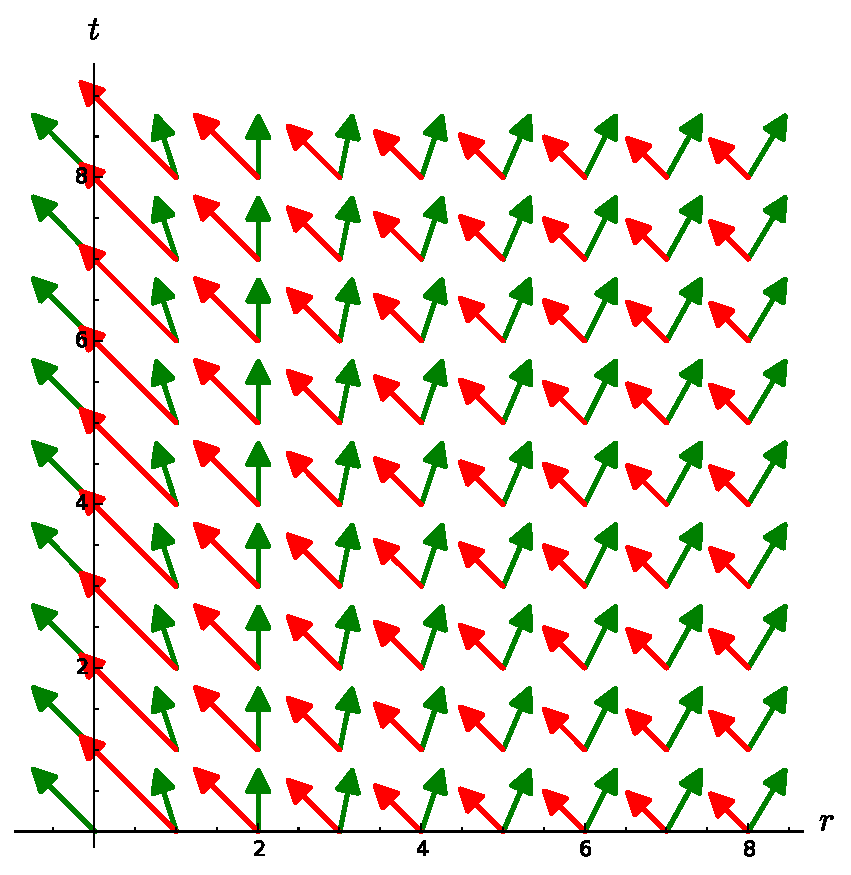
\includegraphics[width=0.6\textwidth]{def_plot_lk.pdf}}
\caption[]{\label{f:def:Schw_hor_lk} \footnotesize
Null vector fields $\wl$ (green) and $\w{k}$ (red) corresponding to
Example~\ref{x:def:Schw_hor5} (Schwarzschild horizon).
The plot is a 2-dimensional slice $\th=\mathrm{const}$ and $\ph=\mathrm{const}$
of the spacetime $\M$, with $t$ and $r$ labelled in units of $m$.
Note that
since $\w{k}$ diverges at $r=0$ [cf. Eq.~(\ref{e:def:k_Schw_hor})], it is not represented there.}
\end{figure}

\begin{example}[Schwarzschild horizon] \label{x:def:Schw_hor5}
For the Schwarzschild horizon case, we deduce from the metric (\ref{e:def:Schw_metric})
and the expression (\ref{e:def:wl_Schw_hor}) for $\wl$ that the null
vector $\w{k}$ orthogonal to the sphere $\Sp$ introduced
in Example~\ref{x:def:Schw_hor4} and obeying $\w{k}\cdot\wl = -1$
is
\be
\label{e:def:k_Schw_hor}
    \w{k} = \left(\frac{1}{2} + \frac{m}{r} \right) \wpar_t
        - \left(\frac{1}{2} + \frac{m}{r} \right) \wpar_r .
\ee
The vector field $\w{k}$ is depicted in Fig.~\ref{f:def:Schw_hor_lk}.
We have (cf. Appendix~\ref{s:sam})
\be \label{e:def:l_k_forms_Schw_hor}
    \uu{\el} = \frac{2m-r}{2m+r} \, \dd t  + \dd r
    \qquad\mbox{and}\qquad
    \uu{k} = - \left(\frac{1}{2} + \frac{m}{r} \right) \dd t
        - \left(\frac{1}{2} + \frac{m}{r} \right) \dd r ,
\ee
so that Eq.~(\ref{e:def:q_g_k_l}) leads to the following components of $\w{q}$
in terms of the 3+1 Eddington-Finkelstein coordinates $x^\alpha=(t,r,\th,\ph)$:
\be \label{e:def:q_Schw_hor}
    q_{\alpha\beta} = \left(
    \begin{array}{cccc}
    0 & 0 & 0 & 0 \\
    0 & 0 & 0 & 0 \\
    0 & 0 & r^2 & 0 \\
    0 & 0 & 0 & r^2\sin^2\th
    \end{array} \right) .
\ee
\end{example}

Having extended the definition of $\w{q}$ via (\ref{e:def:q_g_k_l}), we notice
that the metric dual\footnote{See Eq.~(\ref{e:bas:arrow_endo}) of
Appendix~\ref{s:bas} for the explanation of the arrow notation.}
 of $\w{q}$, i.e. the tensor of type $(1,1)$ defined by
by
\be \label{e:def:q_proj}
    \vw{q} := \mathrm{Id} + \wl\otimes \uu{k} + \w{k}\otimes \uu{\el},
\ee
or, in index notation,
\[
    q^\alpha_{\ \, \beta} = \delta^\alpha_{\ \, \beta}
        + \el^\alpha \, k_\beta + k^\alpha \, \wl_\beta ,
\]
is nothing but the \defin{orthogonal projector} onto the cross-section $\Sp$:
\be
    \forall \w{v}\in T_p\M, \quad \vw{q}(\w{v}) = \w{v}^\parallel .
\ee
The demonstration follows from the decomposition
$\w{v} = \w{v}^\parallel + v^0 \wl + v^1 \w{k}$ used above.
In particular, we have
\be
    \vw{q}(\wl) = 0 \quad\mbox{and}\quad \vw{q}(\w{k}) = 0 .
\ee

%%%%

As stressed by (\ref{e:def:TSperp_Span_k_l}), $(\wl,\w{k})$ forms a null
basis\index{null!basis}\index{basis!null --} of $T_p^\perp\Sp$. One can construct
from it an \emph{orthonormal} basis $(\w{n},\w{s})$ as follows:
\be \label{e:def:ns_lk}
    \left\{ \begin{array}{lcl}
        \w{n} & = & \frac{1}{2} \wl + \w{k} \\
        \w{s} & = & \frac{1}{2} \wl - \w{k} .
        \end{array}\right.
\ee
This system is easily inverted:
\be \label{e:def:lk_ns}
    \left\{ \begin{array}{lcl}
        \wl & = & \w{n} + \w{s} \\
        \w{k} & = & \frac{1}{2} \left( \w{n} - \w{s} \right).
        \end{array}\right.
\ee
Since $\wl\cdot\wl=0$, $\w{k}\cdot\w{k}=0$ and $\wl\cdot\w{k}=-1$, it is
easy to check that:
\be
    \w{n}\cdot\w{n}=-1,\quad \w{s}\cdot\w{s}=1 \quad\mbox{and}\quad
    \w{n}\cdot\w{s}=0.
\ee
In other words, $(\w{n},\w{s})$ is an orthonormal basis\index{orthonormal!basis}\index{basis!orthonormal --} of
the Lorentzian plane $(T_p^\perp\Sp,\w{g})$; in particular:
\be
    T_p^\perp\Sp = \mathrm{Span}\left( \w{n}, \w{s} \right) .
\ee

If we substitute (\ref{e:def:lk_ns}) for $\wl$ and $\w{k}$ in (\ref{e:def:q_g_k_l}),
we get
\[
    \w{q} = \w{g} + \frac{1}{2} (\uu{n}+\uu{s})\otimes(\uu{n}-\uu{s})
    + \frac{1}{2} (\uu{n}-\uu{s})\otimes(\uu{n}+\uu{s}) .
\]
Expanding and simplifying results in
\be
    \w{q} = \w{g} + \uu{n}\otimes\uu{n} - \uu{s}\otimes\uu{s} .
\ee

\begin{figure}
\centerline{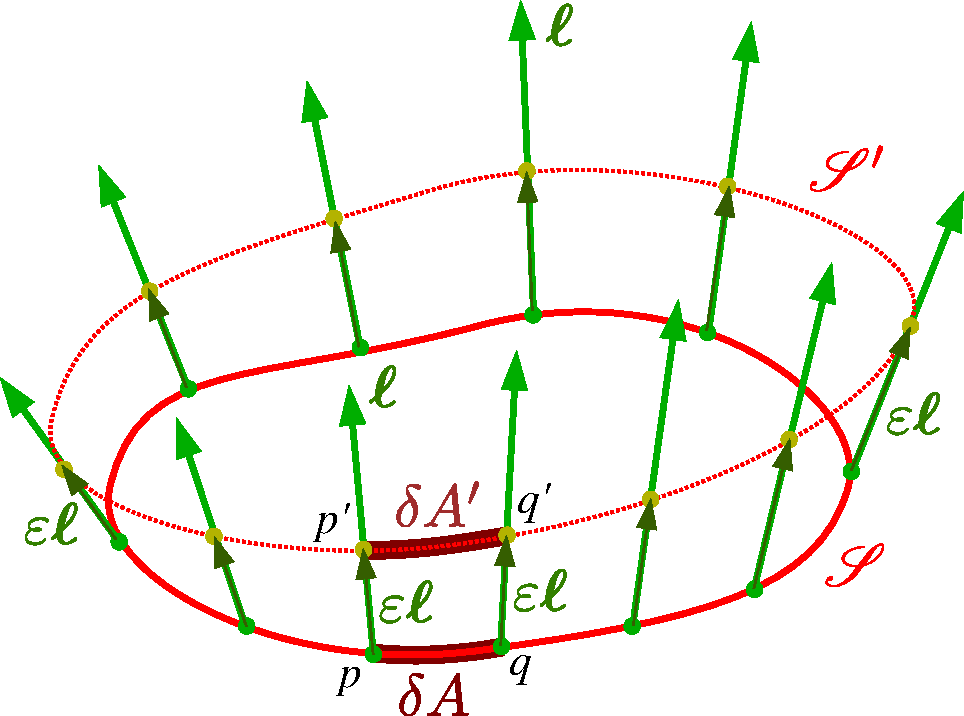
\includegraphics[width=0.6\textwidth]{def_expansion.pdf}}
\caption[]{\label{f:def:expansion} \footnotesize
Lie dragging of the surface $\Sp$ along $\wl$ by the small parameter $\varepsilon$.
$\Sp$ is drawn as a 1-dimensional submanifold, while it is actually a
$(n-2)$-dimensional one, $n$ being the spacetime dimension.}
\end{figure}

\subsection{Expansion along the null normal}

Let us define the expansion of the cross-section $\Sp$ along the vector
field $\wl$ as follows. Given an infinitesimal parameter $\varepsilon\geq 0$, take a point
$p\in \Sp$ and displace it by the (infinitesimal) vector $\varepsilon \wl$, thereby getting
a nearby point $p_\varepsilon$ (cf. Fig.~\ref{f:def:expansion}).
Since $\wl$ is tangent to $\Hor$ and $p\in\Hor$, we have $p_\varepsilon\in\Hor$.
By repeating this for each point in $\Sp$,
keeping the value of $\varepsilon$ fixed, we define a new codimension-2 surface,
$\Sp_\varepsilon$ say cf. Fig.~\ref{f:def:expansion}). One says that $\Sp_\varepsilon$ is obtained
from $\Sp$ by \defin{Lie dragging along $\wl$ by the parameter $\varepsilon$}\index{Lie!dragging}.
Note that $\Sp_0 = \Sp$.
Since $p_\varepsilon\in\Hor$ for every $p\in\Sp$, we have $\Sp_\varepsilon\subset \Hor$.
Because the null direction $\wl$ is transverse to $\Sp_\varepsilon$ by construction, it
follows that $\Sp_\varepsilon$ is spacelilke (cf. the lemma in Sec.~\ref{s:def:spacelike_sections}).

At each point $p\in\Sp$, the \defin{expansion of $\Sp$ along $\wl$} is defined from the
rate of change $\theta_{(\wl)}$ of the area\footnote{We are using the words
\emph{area} and \emph{surface} even if $n-2 \not= 2$, i.e. even if $n\not = 4$,
being aware that for $n=3$ the words \emph{length} and \emph{line} would
be more appropriate, as well as \emph{volume} for $n=5$.}
 $\delta A$ of an element of surface $\delta S$ of
$\Sp$ around $p$:
\be \label{e:def:def_expansion}
    \encadre{ \theta_{(\wl)} := \lim_{\varepsilon\rightarrow 0} \frac{1}{\varepsilon}
    \frac{\delta A_\varepsilon - \delta A}{\delta A} }.
\ee
In the above formula, $\delta A_\varepsilon$ stands for the area of the
surface element $\delta S_\varepsilon\subset \Sp_\varepsilon$ that is obtained from $\delta S$ by
Lie dragging along $\wl$ by the parameter $\varepsilon$ (cf. Fig.~\ref{f:def:expansion}).
\begin{remark} \label{r:def:expansion_indpt_S}
The reader may wonder why the expansion is not denoted by something like
$\theta_{(\wl)}(\Sp)$, since its definition depends explicitly on
$\Sp$. We shall show below that, because $\Hor$ is a null hypersurface, $\theta_{(\wl)}$
is actually independent of the choice of the cross-section $\Sp$.
\end{remark}

For concreteness, let us assume that the element of surface $\delta S \subset\Sp$ is a $(n-2)$-dimensional
parallelogram delimited by some infinitesimal displacement vectors
$\D\w{x}_{(2)}$, $\ldots$, $\D\w{x}_{(n-1)}$. The area of $\delta S$ is then
\be \label{e:def:A_wepsS_dx}
    \delta A = \wepsS(\D\w{x}_{(2)},\ldots,\D\w{x}_{(n-1)}),
\ee
where $\wepsS$ is the Levi-Civita tensor\index{Levi-Civita!tensor}
associated with the metric $\w{q}$
in $\Sp$ (cf. Sec.~\ref{s:bas:Levi-Civita_tensor} in Appendix~\ref{s:bas}).
Since $\w{q}$ is the metric induced by $\w{g}$ in $\Sp$ and $(\w{n},\w{s})$
is an orthonormal basis of $T_p^\perp \Sp$, $\wepsS$ is actually the
alternating form induced on $\Sp$ by the spacetime Levi-Civita tensor
$\weps$:
\be \label{e:def:epsS_ns}
    \encadre{ \wepsS = \weps(\w{n},\w{s},\ldots) },
\ee
or, in index notation,
\[
    \epsS_{\alpha_1\cdots\alpha_{n-2}} = \eps_{\mu\nu\alpha_1\cdots\alpha_{n-2}} n^\mu s^\nu .
\]
\begin{proof}
To demonstrate (\ref{e:def:epsS_ns}), it suffices to note that its right-hand side
defines a fully antisymmetric $(n-2)$-linear form on $T_p\Sp$. Since the space
of such forms is 1-dimensional (for $\dim T_p\Sp = n-2$), we have then
necessarily $\weps(\w{n},\w{s},\ldots) = a \wepsS$ for some proportionality factor $a$. Since
$\weps(\w{n},\w{s},\D\w{x}_{(2)},\ldots,\D\w{x}_{(n-1)})$ is the volume
of the $n$-parallelepiped constructed on the vectors $\w{n},\w{s},\D\w{x}_{(2)},\ldots,\D\w{x}_{(n-1)}$ and $\w{n}$ and $\w{s}$ are unit-length vectors for the metric $\w{g}$,
we have
\[
    \weps(\w{n},\w{s},\D\w{x}_{(2)},\ldots,\D\w{x}_{(n-1)}) = \delta A.
\]
This implies that $a=1$, thereby establishing (\ref{e:def:epsS_ns}).
\end{proof}
An alternative expression of $\wepsS$ is obtained by substituting (\ref{e:def:ns_lk})
for $\w{n}$ and $\w{s}$ in (\ref{e:def:epsS_ns}). Thanks to the multilinearity
and antisymmetry of $\weps$, we get
\be
    \encadre{ \wepsS = \weps(\w{k},\wl,\ldots) } .
\ee

Let us consider in some vicinity of $\Sp$ a coordinate system
\[
    x^\alpha = \left(\varepsilon, u, x^2,\ldots, x^{n-1}\right)
\]
that is adapted to $\Sp$ and $\wl$ in the sense that
\be \label{e:def:l_dsdeps}
    \wl = \der{}{\varepsilon}
\ee
and the points of $\Sp$ are defined by $(\varepsilon,u) = (0,0)$.
Then, from the very definition of the Lie dragging of $\Sp$ along $\wl$, we
have
\be
    \Sp_\varepsilon = \left\{ p\in\M,\quad  (x^0(p), x^1(p)) = (\varepsilon,0)
                        \right\}
\ee
and  $x^a = (x^2,\ldots, x^{n-1})$ can  be viewed as a coordinate system\footnote{
Let us recall that according to the convention stated in Sec.~\ref{s:def:spacelike_sections},  Latin indices from the beginning of the alphabet, $a$, $b$, etc. range from $2$
to $n-1$.} on each surface $\Sp_\varepsilon$.
Let us choose the $n-2$ infinitesimal displacement vectors in (\ref{e:def:A_wepsS_dx})
along the coordinate lines of this system:
\be
    \D x_{(i)}^a = (\underbrace{0,\ldots,0}_{i-2},\D x^i,
                    \underbrace{0,\ldots,0}_{n-1-i}), \qquad
                    2\leq i \leq n-1 .
\ee
Then expression~(\ref{e:def:A_wepsS_dx}) for the area of $\delta S$ becomes
\bea
    \delta A & = & \epsS_{a_1 \cdots a_{n-2}} \, \D x_{(2)}^{a_1} \cdots \D x_{(n-1)}^{a_{n-2}}
                    \nonumber \\
            & = & \epsS_{2\cdots(n-1)} \, \D x^2 \cdots \D x^{n-1} \nonumber \\
     \delta A  & = & \sqrt{q} \, \D x^2 \cdots \D x^{n-1} , \label{e:def:A_sqrt_q}
\eea
where we have used (\ref{e:bas:eps_sqrt_g}) for the components of the
Levi-Civita tensor $\wepsS$, $q$ standing for the determinant of the metric
$\w{q}$ with respect to the coordinates $(x^2,\ldots,x^{n-1})$.
By the very definition of the Lie dragging, the surface element
$\delta S_\varepsilon$ on $\Sp_\varepsilon$
is defined by the same values of the coordinates $(x^2,\ldots, x^{n-1})$
as $\delta S$. In particular, the small coordinate increments $\D x^2$, ..., $\D x^{n-1}$
take the same values as on $\Sp$. Therefore, the area of $\delta S_\varepsilon$
is
\be \label{e:def:A_eps_sqrt_q}
    \delta A_\varepsilon = \sqrt{q(\varepsilon)} \, \D x^2 \cdots \D x^{n-1} ,
\ee
where $q(\varepsilon)$ stands for the determinant of the components of the
metric $\w{q}(\varepsilon)$ induced by $\w{g}$ on $\Sp_\varepsilon$. Since
$\Sp_\varepsilon$ is spacelike (cf. above), $\w{q}(\varepsilon)$ is positive definite, so
that $q(\varepsilon)\geq 0$.

In view of (\ref{e:def:A_sqrt_q})-(\ref{e:def:A_eps_sqrt_q}), the definition (\ref{e:def:def_expansion})
of the expansion of $\Sp$ along $\wl$ can be rewritten as
\[
    \theta_{(\wl)} = \lim_{\varepsilon\rightarrow 0} \frac{1}{\varepsilon}
    \frac{\sqrt{q(\varepsilon)} - \sqrt{q(0)}}{\sqrt{q(0)}} .
\]
We recognize the derivative of the function $\varepsilon \mapsto \ln \sqrt{q(\varepsilon)}=
1/2\, \ln q(\varepsilon)$ at $\varepsilon=0$:
\be \label{e:def:theta_deps_ln_q}
     \theta_{(\wl)} = \frac{1}{2} \frac{\D}{\D\varepsilon}  \ln q .
\ee
Given that $\Sp_\varepsilon$ is deduced from $\Sp$ by a Lie dragging along $\wl$
and $\varepsilon$ is the parameter associated with $\wl$ [cf. Eq.~(\ref{e:def:l_dsdeps})], we may
rewrite this formula as the Lie derivative of $\ln q$ along $\wl$:
\be \label{e:def:theta_Lie_ln_q}
    \encadre{ \theta_{(\wl)} = \frac{1}{2} \Lie{\el} \ln q }.
\ee
\begin{example}[light cone] \label{x:def:light_cone6}
For the light cone in Minkowski spacetime,
it is easy to evaluate $\theta_{(\wl)}$ by means of the spherical coordinates
introduced in Example~\ref{x:def:light_cone5}, since these coordinates are adapted to the
surface $\Sp$, the metric of $\Sp$ being $q_{ab} \D x^a \D x^b = r^2 \D \theta^2
+ r^2\sin^2\theta \D \ph^2$ [cf. Eq.~(\ref{e:def:q_light_cone_spher})].
We have then  $q = \det(q_{ab}) = r^4\sin^2\theta$. Moreover the parameter $\varepsilon$
can be chosen as $\varepsilon = t - t_0$ since $t$ is an (affine) parameter
associated with $\wl$ (cf. Example~\ref{x:def:light_cone3}). Given that
$t=r$ on $\Hor$, we have $\varepsilon = r - t_0$, so that (\ref{e:def:theta_deps_ln_q})
yields
\[
    \theta_{(\wl)} = \frac{1}{2} \frac{\D}{\D r}  \ln q =
         \frac{1}{2} \frac{\D}{\D r} \left( 4 \ln r + 2 \ln\sin\theta \right) ,
\]
i.e.
\be \label{e:def:theta_light_cone}
    \theta_{(\wl)} = \frac{2}{r} .
\ee
\end{example}

\begin{example}[Schwarzschild horizon] \label{x:def:Schw_hor6}
As above, we have $q = r^4\sin^2\th$ [cf. Eq.~(\ref{e:def:q_S_Schw_hor})],
so that (\ref{e:def:theta_Lie_ln_q}) yields
\bea
    \theta_{(\wl)} & =& \frac{1}{2} \Lie{\el} \ln q = \frac{1}{2} \el^\mu \der{}{x^\mu} \ln q
        = \underbrace{\der{}{t} \ln (r^2\sin\th)}_{0}
            + \frac{r-2m}{r+2m} \der{}{r} \ln (r^2\sin\th) \nonumber \\
       & = & \frac{2}{r} \frac{r-2m}{r+2m}  . \label{e:def:theta_Schw_hor_u}
\eea
where we have used
(\ref{e:def:wl_Schw_hor}) for the components $\el^\mu$.
The above expression is valid for any null hypersurface $\Hor_u$. For the
specific case of the Schwarzschild horizon, $r=2m$ and (\ref{e:def:theta_Schw_hor_u})
yields a vanishing expansion:
\be \label{e:def:theta_Schw_hor}
    \theta_{(\wl)} = 0 .
\ee
Note that for large $r$, Eq.~(\ref{e:def:theta_Schw_hor_u}) yields
$\theta_{(\wl)} \sim 2/r$, i.e. we recover the flat
spacetime result (\ref{e:def:theta_light_cone}), which is consistent with the
fact that for large $r$, $\Hor_u$ is closed to a Minkowskian light cone
(cf. Fig.~??). Note also that Eq.~(\ref{e:def:theta_Schw_hor_u}) yields
$\theta_{(\wl)} <0$ for $r<2m$ and $\theta_{(\wl)} >0$ for $r>2m$. These
expansion values are in agreement with what can be infered from Fig.~\ref{f:def:Schw_hor_lk},
since $r$ is directly related to the area of the cross-sections of $\Hor$:
$A = 4\pi r^2$ from Eq.~(\ref{e:def:q_Schw_hor}).
\end{example}

Using the general law of variation of a derminant, as given by Eq.~(\ref{e:bas:variation_det})
in Appendix~\ref{s:bas}, Eq.~(\ref{e:def:theta_Lie_ln_q}) can be rewritten as
\[
    \theta_{(\wl)} = \frac{1}{2} \, \mathrm{tr} \left(Q^{-1} \times \Lie{\el} Q \right) ,
\]
when $Q$ is the matrix representing the components of $\w{q}$ with respect to the
coordinates $(x^a) = (x^2,\ldots, x^{n-1})$. In index notation, we have
$Q = (q_{ab})$ and $Q^{-1} = (q^{ab})$. Hence
\be \label{e:def:theta_q_ab}
    \encadre{ \theta_{(\wl)} = \frac{1}{2} \, q^{ab} \Liec{\el} q_{ab} } .
\ee
One may wonder about the link between the Lie derivative along $\wl$ of the $(n-2)$-metric
$\w{q}$ of the cross-sections $\Sp_\varepsilon$, which appears above, and
the Lie derivative along $\wl$ of the spacetime extension $\w{q}$ defined by
(\ref{e:def:q_g_k_l}). For the sake of clarity, let us denote here the latter
by $\w{\bar q}$. More precisely, we may consider that $\w{\bar q}$ is a
field defined in some neighbourhood of the portion of $\Hor$ sliced by
$\bigcup_{\varepsilon} \Sp_\varepsilon$ via (\ref{e:def:q_g_k_l}), with $\w{k}$
defined at each point $p\in\Sp_\varepsilon$ as the unique null vector of
$T_p^\perp\Sp_\varepsilon$ obeying $\wl\cdot\w{k}=-1$.
Let $\w{u}$ and $\w{v}$ be vector fields on $\Hor$ that are tangent
to the cross-sections $\Sp_\varepsilon$. Applying the bilinear form
$\Lie{\el}\w{\bar q}$ to them and using the Leibniz rule to expand
$\Lie{\el} \left[ \w{\bar q}(\w{u},\w{v}) \right]$ yields
\be \label{e:def:Lie_l_bar_q}
     \Lie{\el} \w{\bar q} \, (\w{u},\w{v}) = \Lie{\el} \left[ \w{\bar q}(\w{u},\w{v}) \right]
        - \w{\bar q}\left(\Lie{\el}\w{u},\w{v}\right)
         - \w{\bar q}\left(\w{u},\Lie{\el}\w{v}\right) .
\ee
Now, since $\w{u}$ and $\w{v}$ are tangent to $\Sp_\varepsilon$, we may
write $\w{\bar q}(\w{u},\w{v}) = \w{q}(\w{u},\w{v})$. Moreover, by the very
definition of a Lie derivative of a vector field (cf. Sec.~\ref{s:bas:Lie}
in Appendix~\ref{s:bas}) and the fact that the cross-sections
$\Sp_\varepsilon$ are Lie-dragged along $\wl$, the vectors
$\Lie{\el}\w{u}$ and $\Lie{\el}\w{v}$ are also tangent to $\Sp_\varepsilon$.
Therefore, we have
\[
    \w{\bar q}\left(\Lie{\el}\w{u},\w{v}\right) = \w{q} \left(\Lie{\el}\w{u},\w{v}\right)
    \quad\mbox{and}\quad
    \w{\bar q}\left(\w{u},\Lie{\el}\w{v}\right) = \w{q}\left(\w{u},\Lie{\el}\w{v}\right)
\]
as well. Thus, we may rewrite (\ref{e:def:Lie_l_bar_q}) as
\[
     \Lie{\el} \w{\bar q} \, (\w{u},\w{v}) = \Lie{\el} \left[ \w{q}(\w{u},\w{v}) \right]
        - \w{q}\left(\Lie{\el}\w{u},\w{v}\right)
         - \w{q}\left(\w{u},\Lie{\el}\w{v}\right) .
\]
The right-hand side being identical to what would be obtained by expressing
$\Lie{\el} \w{q} \, (\w{u},\w{v})$ via the Leibniz rule. Hence we conclude
that
\[
    \Lie{\el} \w{\bar q} \, (\w{u},\w{v}) = \Lie{\el} \w{q} \, (\w{u},\w{v}) .
\]
Since this identity holds for a pair $(\w{u},\w{v})$ of vectors tangent
to $\Sp_\varepsilon$, we may express it for any pair of vectors, i.e. not
necessarily tangent to $\Sp_\varepsilon$ by introducing the orthogonal
projector $\vw{q}$ onto $\Sp_\varepsilon$ [cf. Eq.~(\ref{e:def:q_proj})]:
\[
    \Lie{\el} \w{\bar q} \, (\vw{q}(\w{u}),\vw{q}(\w{v})) =
    \Lie{\el} \w{q} \, (\vw{q}(\w{u}),\vw{q}(\w{v})) .
\]
Using index notation, this is equivalent to
\[
    \Liec{\el} {\bar q}_{\mu\nu} \, {\bar q}^\mu_{\ \, \alpha} {\bar q}^\nu_{\ \, \beta} =
        \Liec{\el} {q}_{ab} \, {\bar q}^a_{\ \, \alpha} {\bar q}^b_{\ \, \beta} .
\]
Taking the trace with respect to $\w{g}$, we get
\[
    \Liec{\el} {\bar q}_{\mu\nu} \, {\bar q}^\mu_{\ \, \sigma} {\bar q}^{\nu\sigma} =
        \Liec{\el} {q}_{ab} \, {\bar q}^a_{\ \, \sigma} {\bar q}^{b\sigma} .
\]
Now, since $\w{\bar q}$ is symmetric and $\vw{q}$ is a projector,
${\bar q}^\mu_{\ \, \sigma} {\bar q}^{\nu\sigma} = {\bar q}^\mu_{\ \, \sigma} {\bar q}^{\sigma\nu}
 = {\bar q}^{\mu\nu}$. Similarly, ${\bar q}^a_{\ \, \sigma} {\bar q}^{b\sigma} = {\bar q}^{ab}$.
Hence
\[
    {\bar q}^{\mu\nu} \Liec{\el} {\bar q}_{\mu\nu} = {\bar q}^{ab}  \Liec{\el} {q}_{ab}
    = q^{ab}  \Liec{\el} {q}_{ab} ,
\]
where the second equality follows from
${\bar q}^{ab}  = q^{ab}$.
Hence we may rewrite (\ref{e:def:theta_q_ab}) as
\be \label{e:def:theta_q_munu}
   \encadre{ \theta_{(\wl)} = \frac{1}{2} \, q^{\mu\nu} \Liec{\el} q_{\mu\nu} }.
\ee
Note that we have dropped the bar over $q$, i.e. we revert to the previous notation.

Substituting (\ref{e:def:q_g_k_l}) for $q_{\mu\nu}$, and using the Leibniz rule, we get
\[
    \theta_{(\wl)} = \frac{1}{2} \, q^{\mu\nu}  \left(
            \Liec{\el} g_{\mu\nu} + \Liec{\el}  \el_\mu \; k_\nu + \el_\mu \, \Liec{\el} k_\nu
           + \Liec{\el} k_\mu \; \el_\nu + k_\mu \, \Liec{\el} \el_\nu \right) .
\]
If we express the Lie derivative $\Liec{\el} g_{\mu\nu}$ in terms of the
covariant derivative $\wnab$ via Eq.~(\ref{e:bas:Lie_der_comp_nab}) of
Appendix~{\ref{s:bas}, we get
\[
    \Liec{\el} g_{\mu\nu} = \el^\sigma \underbrace{\nabla_\sigma g_{\mu\nu}}_{0}
        + \underbrace{g_{\sigma\nu} \nabla_\mu \el^\sigma}_{\nabla_\mu \el_\nu}
        + \underbrace{g_{\mu\sigma} \nabla_\nu \el^\sigma}_{\nabla_\nu \el_\mu}
       = \nabla_\mu \el_\nu + \nabla_\nu \el_\mu .
\]
Moreover, since $\wl$ and $\w{k}$ are orthogonal to $\Sp$, we have
\[
    q^{\mu\nu} \el_\nu = 0 \quad\mbox{and}\quad
    q^{\mu\nu} k_\nu = 0 .
\]
Hence we end up with
\[
    \theta_{(\wl)} = \frac{1}{2} \, q^{\mu\nu}  \left( \nabla_\mu \el_\nu + \nabla_\nu \el_\mu
        \right) ,
\]
i.e. since $q^{\mu\nu}$ is symmetric,
\be
    \encadre{ \theta_{(\wl)} = q^{\mu\nu} \nabla_\mu \el_\nu } .
\ee

We can transform further this relation by expressing $q^{\mu\nu}$ via (\ref{e:def:q_g_k_l}):
\bea
    \theta_{(\wl)} & = & \left( g^{\mu\nu} + \el^\mu k^\nu + k^\mu \el^\nu \right)
        \nabla_\mu \el_\nu  \nonumber \\
        & = & \nabla_\mu \el^\mu + k^\nu \underbrace{\el^\mu  \nabla_\mu \el_\nu }_{\kappa \el_\nu}
            + k^\mu \el^\nu  \nabla_\mu \el_\nu \nonumber \\
        & = & \nabla_\mu \el^\mu + \kappa \underbrace{k^\nu \el_\nu}_{-1}
            + \frac{1}{2} \underbrace{k^\mu \nabla_\mu (\el_\nu \el^\nu)}_{0}
            \nonumber \\
        & = & \nabla_\mu \el^\mu - \kappa , \label{e:def:theta_div_l_index}
\eea
where we have used respectively the properties (\ref{e:def:wl_geod_kappa}),
(\ref{e:def:el_nab_el_zero}) and (\ref{e:def:k_el_minus_one}).
Denoting the divergence of $\wl$ by $\wnab\cdot\wl = \nabla_\mu \el^\mu$, we
have then
\be \label{e:def:theta_div_l}
    \encadre{\theta_{(\wl)} = \wnab\cdot\wl - \kappa } .
\ee
\begin{remark} \label{r:def:theta_div_l}
Contrary to $\theta_{(\wl)}$ or $\kappa$, the quantity $\wnab\cdot\wl$ depends
on the extension of $\wl$ outside $\Hor$ (cf. the discussion in Sec.~\ref{s:def:null_normal}).
For Eq.~(\ref{e:def:theta_div_l}) to hold, we have supposed that $\wl$ remains null
outside $\Hor$, so that $k^\mu\nabla_\mu(\el_\nu \el^\nu)$, which is a
derivative in a direction transverse to $\Hor$, could be set to zero
in the computation leading to (\ref{e:def:theta_div_l_index}).
\end{remark}

\begin{example}[light cone]  \label{x:def:light_cone7}
$\wnab\cdot\wl$ is easily computed by taking the trace of
(\ref{e:def:nab_l_light_cone}) and we have $\kappa=0$ (cf. Example~\ref{x:def:light_cone3}),
so that (\ref{e:def:theta_div_l}) yields
\[
    \theta_{(\wl)} = \frac{2(x^2+y^2+z^2)}{r^3} = \frac{2}{r} .
\]
Hence we recover the result obtained in Example~\ref{x:def:light_cone6}.
\end{example}

\begin{example}[Schwarzschild horizon] \label{x:def:Schw_hor7}
Here also, $\wnab\cdot\wl$ is easily computed by taking the trace of
(\ref{e:def:nab_l_Schw_hor}):
\[
    \wnab\cdot\wl = \frac{m}{r^2} + \frac{m}{r^2} \frac{3r^2-4m(r+m)}{(r+2m)^2}
        + 2\frac{r-2m}{r(r+2m)} =
    \frac{2(r^2 + 2mr - 4m^2)}{r(r+2m)^2} .
\]
Given the value $\kappa= 4m/(r+2m)^2$ found in Example~\ref{x:def:Schw_hor3},
formula (\ref{e:def:theta_div_l}) leads to
\[
     \theta_{(\wl)} = \frac{2(r^2 + 2mr - 4m^2) - 4mr}{r(r+2m)^2} = \frac{2(r^2-4m^2)}{r(r+2m)^2}
     = \frac{2}{r} \frac{r-2m}{r+2m} .
\]
Hence we recover the result (\ref{e:def:theta_Schw_hor_u}).
\end{example}

\begin{figure}
\vspace{5cm}
%\centerline{\includegraphics[width=0.6\textwidth]{}}
\caption[]{\label{f:def:two_cross_sections} \footnotesize
Two cross-sections $\Sp$ and $\Sp'$ through the same point $p$ of $\Hor$.}
\end{figure}



We notice that the right-hand side of (\ref{e:def:theta_div_l}) is independent of the
explicit choice of the cross-section $\Sp$: clearly both $\wnab\cdot\wl$
and $\kappa$ depends only on the null normal $\wl$ of $\Hor$. This justifies
the notation $\theta_{(\wl)}$, which does not refer to $\Sp$
(cf. Remark~\ref{r:def:expansion_indpt_S} in page~\pageref{r:def:expansion_indpt_S}).
This can be understood geometrically as follows. Let $p\in\Hor$ be a
point where one would like to evaluate $\theta_{(\wl)}$. Let $\Sp$ and $\Sp'$
be two distinct cross-sections of $\Hor$ going through $p$
(cf. Fig.~\ref{f:def:two_cross_sections}). Let $q$ be a point of $\Sp$ infinitely close to $p$ and let $q'$
be the point of $\Sp'$ located on the same null geodesic generator as $q$,
i.e. $\vec{qq'} = \varepsilon \wl$, with $\varepsilon$ infinitely small.
Let $\D\w{x}$ (resp. $\D\w{x'}$) be the infinitesimal vector connecting
$p$ to $q$ (resp. $p$ to $q'$). We have then
\[
\D\w{x'} = \D\w{x} + \varepsilon \wl ,
\]
the scalar square of which is
\[
    \D\w{x'}\cdot\D\w{x'} =\D\w{x}\cdot\D\w{x}
            + 2 \varepsilon \underbrace{\D\w{x}\cdot \wl}_{0}
            + \underbrace{\wl\cdot \wl}_{0},
\]
where we have used the fact that $\wl$ is normal to any vector tangent to $\Hor$,
such as $\D\w{x}$ and $\wl$ itself. Hence
\[
    \D\w{x'}\cdot\D\w{x'} = \D\w{x}\cdot\D\w{x} .
\]
In other words, the lengths of all segments from $p$ do not depend
on the cross-section in which they are taken, provided their second end
lies on the same null geodesic generator of $\Hor$. It follows that all infinitesimal surfaces
$\delta S$ around $p$ that are enclosed in a tube made of null geodesic generators have the same
area $\delta A$. Hence the expansion $\theta_{(\wl)}$ at $p$
does not depend on the choice of $\delta S$, i.e. of the cross-section
$\Sp$ through $p$.
We conclude that
\begin{greybox}
The expansion $\theta_{(\wl)}$ depends only on the choice of the null
normal $\wl$ on the null hypersurface $\Hor$.
\end{greybox}
For this reason, from now on, we shall call $\theta_{(\wl)}$
the \defin{expansion of the null hypersurface $\Hor$ along $\wl$}\index{expansion!of a null hypersurface}.

The dependency of the expansion on $\wl$ is given by the following
behaviour under a rescaling of $\wl$:
\be \label{e:def:rescale_lambda}
   \wl' = \alpha \wl \ \Longrightarrow \ \theta_{(\wl')} = \alpha \theta_{(\wl)} ,
\ee
where $\alpha$ is any positive scalar field on $\Hor$. This follows immediately
from the expression (\ref{e:def:theta_Lie_ln_q}) of $\theta_{(\wl)}$, given
that the metric $\w{q}$ is independent of $\wl$ and
$\w{\Liesymbol}_{\alpha\wl}\,\ln q = \alpha \Lie{\wl}\ln q$.
\begin{remark}
The reader may check that the rescaling laws (\ref{e:def:rescale_kappa})
and (\ref{e:def:rescale_lambda}) for respectively $\kappa$ and $\theta_{(\wl)}$
are compatible with the expression (\ref{e:def:theta_div_l}) of $\theta_{(\wl)}$,
given that $\wnab\cdot \wl' = \alpha\wnab\cdot\wl + \wnab_{\wl} \alpha$.
\end{remark}

Let us gather all the expressions of the expansion $\theta_{(\wl)}$ obtained
so far:
\be \label{e:def:theta_l_all}
    \encadre{ \theta_{(\wl)} = \lim_{\varepsilon\rightarrow 0} \frac{1}{\varepsilon}
    \frac{\delta A_\varepsilon - \delta A}{\delta A}
        = \frac{1}{2} \Lie{\el} \ln q
        = \frac{1}{2} \, q^{\mu\nu} \Liec{\el} q_{\mu\nu}
        = q^{\mu\nu} \nabla_\mu \el_\nu
        = \wnab\cdot\wl - \kappa } ,
\ee
with the reminder that the last expression is valid insofar as the vector field $\wl$ is
null in some entire open neighbourhood of $\Hor$ (and not only on $\Hor$), as
stressed in Remark~\ref{r:def:theta_div_l}.

\subsection{Deformation rate and shear tensor}

Let us consider a cross-section $\Sp$ of the null hypersurface $\Hor$.
The \defin{deformation rate}\index{deformation rate} $\w{\Theta}$ of $\Sp$ is defined from the Lie
derivative of the induced metric $\w{q}$ of $\Sp$ along $\wl$ as
\be \label{e:def:Theta}
    \w{\Theta} := \frac{1}{2} \vw{q}^* \Lie{\el} \w{q} ,
\ee
where $\vw{q}^*$ stands for the action of the orthogonal projector $\vw{q}$
onto $\Sp$ on the bilinear form $\Lie{\el} \w{q}$.
This action extends $\Lie{\el} \w{q}$, which is defined a priori on
vectors of $T_p\Sp$ to all vectors of $T_p\M$, for any $p\in\Sp$, via
\be
    \forall (\w{u},\w{v}) \in T_p\M \times T_p\M, \quad
         \vw{q}^* \Lie{\el} \w{q}\,  (\w{u}, \w{v}) =
         \Lie{\el} \w{q} \left( \vw{q}(\w{u}), \vw{q}(\w{v}) \right) .
\ee
Accordingly, the index-notation version of (\ref{e:def:Theta}) is
\be \label{e:def:Theta_index}
    \Theta_{\alpha\beta} = \frac{1}{2} q^\mu_{\ \, \alpha} q^\nu_{\ \, \beta}
            \Liec{\el} q_{\mu\nu} .
\ee
Since $\w{q}$ is symmetric, it is clear from the above definition that
$\w{\Theta}$ is a symmetric bilinear form.

Expressing the Lie derivative in terms of the covariant derivative
$\wnab$ via Eq.~(\ref{e:bas:Lie_der_comp_nab}) of Appendix~{\ref{s:bas}
and using expression (\ref{e:def:q_g_k_l}) of $\w{q}$, we get
\bea
    \Theta_{\alpha\beta} & = & \frac{1}{2} q^\mu_{\ \, \alpha} q^\nu_{\ \, \beta}
        \left( \el^\sigma \nabla_\sigma q_{\mu\nu}
            + q_{\sigma\nu}\nabla_\mu \el^\sigma
            + q_{\mu\sigma}\nabla_\nu \el^\sigma \right) \nonumber \\
            & = & \frac{1}{2} q^\mu_{\ \, \alpha} q^\nu_{\ \, \beta} \Big[
                \el^\sigma \left( \nabla_\sigma \el_\mu k_\nu
                    + \el_\mu \nabla_\sigma k_\nu +  \nabla_\sigma k_\mu \el_\nu
                    + k_\mu \nabla_\sigma \el_\nu \right) \nonumber \\
            & & \qquad\qquad + \nabla_\mu \el_\nu + k_\nu \underbrace{\el_\sigma \nabla_\mu \el^\sigma}_{0}
                + k_\sigma \el_\nu \nabla_\mu \el^\sigma  + \nabla_\nu \el_\mu + \el_\mu k_\sigma \nabla_\nu \el^\sigma
                + k_\mu \underbrace{\el_\sigma \nabla_\nu \el^\sigma}_{0}
                                    \Big] . \nonumber
\eea
Since $q^\mu_{\ \, \alpha} \el_\mu = 0$ and $q^\mu_{\ \, \alpha} k_\mu = 0$,
the above expression simplifies to
\be
    \Theta_{\alpha\beta}  = q^\mu_{\ \, \alpha} q^\nu_{\ \, \beta} \nabla_\mu \el_\nu .
\ee
Let us substitute (\ref{e:def:q_proj}) for the projector $\vw{q}$:
\[
    \Theta_{\alpha\beta}  = \left(\delta^\mu_{\ \, \alpha}
        + \el^\mu k_\alpha + k^\mu \el_\alpha \right)
        \left(\delta^\nu_{\ \, \beta}
        + \el^\nu k_\beta + k^\nu \el_\beta \right) \nabla_\mu \el_\nu .
\]
Expanding and simplifying (in particular via $\el^\nu \nabla_\mu \el_\nu = 0$)
yields
\be \label{e:def:nab_l_Theta}
   \encadre{ \nabla_\alpha \el_\beta = \Theta_{\alpha\beta}
        + \omega_\alpha \el_\beta - \el_\alpha k^\mu \nabla_\mu \el_\beta },
\ee
with
\be \label{e:def:def_omega}
    \omega_\alpha := - k^\mu \nabla_\alpha \el_\mu - k^\mu k^\nu \nabla_\mu \el_\nu \, \el_\alpha .
\ee
\begin{remark}
The 1-form $\w{\omega}$ is sometimes called the \defin{rotation 1-form} of
the cross-section $\Sp$; see Ref.~\cite{GourgJ06} for details.
\end{remark}

By comparing (\ref{e:def:theta_q_munu}) and (\ref{e:def:Theta_index}), we
notice that the trace of $\w{\Theta}$ is nothing but the expansion
$\theta_{(\wl)}$:
\be
   \encadre{ \theta_{(\wl)} = g^{\mu\nu} \Theta_{\mu\nu} = q^{\mu\nu} \Theta_{\mu\nu} = \Theta^\mu_{\ \, \mu} }.
\ee
The trace-free part of $\w{\Theta}$ is called the \defin{shear tensor}\index{shear!tensor}
of $\Sp$:
\be \label{e:def:def_shear}
    \encadre{ \w{\sigma} := \w{\Theta} - \frac{1}{n-2} \theta_{(\wl)} \, \w{q} } ,
\ee
or, in index notation:
\be
    \sigma_{\alpha\beta} = \Theta_{\alpha\beta} - \frac{1}{n-2} \theta_{(\wl)} \, q_{\alpha\beta} .
\ee
Note that the $1/(n-2)$ factor arises from the trace of $\w{q}$, which is $n-2$,
as easily seen from (\ref{e:def:q_g_k_l}):
\be
    q^\mu_{\ \, \mu} = \underbrace{\delta^\mu_{\ \, \mu}}_{n}
                    + 2 \underbrace{\el^\mu k^\mu}_{-1} = n - 2 .
\ee
By construction, we have thus
\be
    \sigma^\mu_{\ \, \mu} = g^{\mu\nu} \sigma_{\mu\nu} = q^{\mu\nu} \sigma_{\mu\nu} = 0 .
\ee
Note that $\w{\Theta}$ and $\w{\sigma}$ are tensor fields tangent to $\Sp$, in the sense
that
\be \label{e:def:Theta_sigma_tangent}
   \encadre{\forall \w{v}\in T_p^\perp \Sp, \quad \w{\Theta}(\w{v}, .) = \w{\sigma}(\w{v}, .) = 0 },
\ee
with the important special cases $\w{v} = \wl$ and $\w{v} = \w{k}$.

\begin{remark}
Contrary to $\theta_{(\wl)}$, which depends only on $\wl$, the tensor fields
$\w{\Theta}$ and $\w{\sigma}$ depend on the specific choice of the cross-section $\Sp$,
in addition to $\wl$.
\end{remark}

\begin{example}[light cone] \label{x:def:light_cone8}
Let us consider the light cone in Minkowski spacetime described in terms of the
spherical coordinates introduced in Example~\ref{x:def:light_cone5}.
Since the coordinates $(t,\th,\ph)$
are adapted to the vector field $\wl$ (i.e. the $\th$ and $\ph$ are constant
along the field lines of $\wl$ on $\Hor$ and $\wl = \partial/\partial t$ in these
coordinates, in other words, $\el^\alpha=(1,0,0)$), we have [cf. formula~(\ref{e:bas:Lie_adapted})
in Appendix~\ref{s:bas}]
\[
    \Liec{\el} q_{ab} = \der{}{t} q_{ab} = \der{}{r} q_{ab} ,
\]
where the second equality follows from $t=r$ on $\Hor$. Given that
$q_{ab} = \mathrm{diag}(r^2, r^2\sin^2\th)$
[cf. Eq.~(\ref{e:def:q_light_cone_spher})], we obtain
\[
    \Liec{\el} q_{ab} = \left( \begin{array}{cc}
        2 r & 0  \\
        0 & 2 r \sin^2\theta
        \end{array} \right)
        = \frac{2}{r} \, q_{ab} .
\]
Hence (\ref{e:def:Theta}) yields
\[
    \w{\Theta} = \frac{1}{r} \, \w{q} .
\]
Taking the trace, we get immediately $\theta_{(\wl)} = 2/r$, i.e. we recover
the result of Examples~\ref{x:def:light_cone6} and \ref{x:def:light_cone7}.
From (\ref{e:def:def_shear}), we get a vanishing shear:
\[
    \w{\sigma} = 0 .
\]
\end{example}

\begin{example}[Schwarzschild horizon] \label{x:def:Schw_hor8}
The Lie derivative of $\w{q}$, as given by Eq.~(\ref{e:def:q_Schw_hor}),
along $\wl$ is (cf. Appendix~\ref{s:sam} for the computation):
\[
    \Lie{\wl} \w{q} =  2 r \frac{r-2m}{r+2m} \left( \dd\th \otimes \dd\th
        +  \sin^2\th \, \dd\ph \otimes \dd\ph \right) = \frac{2}{r} \frac{r-2m}{r+2m}
            \, \w{q} .
\]
Since $\vw{q}^* \w{q} = \w{q}$, Eq.~(\ref{e:def:Theta}) yields
\[
    \w{\Theta} = \frac{r-2m}{r(r+2m)} \, \w{q} .
\]
This formula is valid for all null hypersurface $\Hor_u$. For the specific
case of the Schwarzschild horizon $\Hor$, $r=2m$ and it reduces to
\be \label{e:def:Theta_zero_Schw_hor}
    \w{\Theta} = 0 .
\ee
\end{example}

\section{Null Raychaudhuri equation} \label{s:def:null_raychaud}

Let us derive an evolution equation for the expansion $\theta_{(\wl)}$.
The starting point is the Ricci identity [Eq.~(\ref{e:bas:Ricci_ident}) in Appendix~\ref{s:bas}]
applied to $\wl$:
\[
   \left(\nabla_\alpha\nabla_\beta
        - \nabla_\beta\nabla_\alpha\right) \el^\gamma
        = R^\gamma_{\ \  \mu \alpha\beta} \, \el^\mu ,
\]
where $R^\gamma_{\ \  \mu \alpha\beta}$ is the Riemann tensor of the metric
$\w{g}$.
Taking the trace on the indices $(\alpha,\gamma)$ and relabelling $\beta\rightarrow\alpha$ yields
\[
    \nabla_\mu \nabla_\alpha \el^\mu - \nabla_\alpha \nabla_\mu \el^\mu =
        R_{\mu\alpha} \el^\mu ,
\]
where $R_{\mu\alpha} = R^\sigma_{\ \  \mu \sigma\alpha}$ is
the Ricci tensor of $\w{g}$.
Substituting Eq.~(\ref{e:def:nab_l_Theta}) for $\nabla_\alpha \el^\mu$ and $\theta_{(\wl)} + \kappa$ for $\nabla_\mu \el^\mu = \wnab\cdot\wl$ [cf. Eq.~(\ref{e:def:theta_div_l})] yields
\[
    \nabla_\mu \left( \Theta_\alpha^{\ \, \mu} + \omega_\alpha \el^\mu - \el_\alpha
        k^\nu \nabla_\nu \el^\mu \right) - \nabla_\alpha \left( \theta_{(\wl)} + \kappa \right) =
        R_{\mu\alpha} \el^\mu .
\]
Expanding the left-hand side and using again Eqs.~(\ref{e:def:theta_div_l}) and
(\ref{e:def:nab_l_Theta}) results in
\bea
    \nabla_\mu \Theta^\mu_{\ \, \alpha} + \el^\mu \nabla_\mu \omega_\alpha
       - \nabla_\alpha \left( \theta_{(\wl)} + \kappa \right)
        + \left( \theta_{(\wl)} + \kappa \right) \omega_\alpha
        - \Theta_{\alpha\mu} k^\nu \nabla_\nu \el^\mu & & \nonumber \\
    - \left( \omega_\mu k^\nu \nabla_\nu \el^\mu
    + \nabla_\mu k^\nu \nabla_\nu \el^\mu + k^\nu \nabla_\mu \nabla_\nu \el^\mu \right)
        \el_\alpha & = & R_{\mu\alpha} \el^\mu . \label{e:def:contract_Ricci_ident}
\eea
The above relation is a 1-form identity. Applying it to the vector field $\wl$
(i.e. contracting with $\el^\alpha$), we get, since $\el_\nu \el^\nu =0$,
\be \label{e:def:Raychaud_step1}
    \el^\nu \nabla_\mu \Theta^\mu_{\ \, \nu} + \el^\nu \el^\mu \nabla_\mu \omega_\nu
        - \el^\mu \nabla_\mu \left( \theta_{(\wl)} + \kappa \right)
        + \left( \theta_{(\wl)} + \kappa \right) \omega_\mu \el^\mu
        = R_{\mu\nu} \el^\mu \el^\nu .
\ee
Now, using $\Theta^\mu_{\ \, \nu}  \el^\nu = 0$ [Eq.~(\ref{e:def:Theta_sigma_tangent})]
and Eq.~(\ref{e:def:nab_l_Theta}), we can write
\bea
    \el^\nu \nabla_\mu \Theta^\mu_{\ \, \nu} & = & \nabla_\mu
    ( \underbrace{\Theta^\mu_{\ \, \nu} \el^\nu}_{0} )
    - \Theta^\mu_{\ \, \nu} \nabla_\mu \el^\nu = - \Theta^{\mu\nu} \nabla_\mu \el_\nu
    = - \Theta^{\mu\nu}  \left( \Theta_{\mu\nu} + \omega_\mu \el_\nu
        - \el_\mu k^\sigma \nabla_\sigma \el_\nu \right) \nonumber \\
    & = & - \Theta^{\mu\nu}  \Theta_{\mu\nu} . \nonumber
\eea
On the other side,
\[
    \el^\nu \el^\mu \nabla_\mu \omega_\nu = \el^\mu \nabla_\mu (\omega_\nu \el^\nu )
        - \omega_\nu \underbrace{\el^\mu \nabla_\mu \el^\nu}_{\kappa \el^\nu}
        = \el^\mu \nabla_\mu (\omega_\nu \el^\nu ) - \kappa \omega_\nu \el^\nu ,
\]
Accordingly Eq.~(\ref{e:def:Raychaud_step1}) becomes
\[
    - \Theta^{\mu\nu}  \Theta_{\mu\nu}  + \el^\mu \nabla_\mu (\omega_\nu \el^\nu )
        - \el^\mu \nabla_\mu \left( \theta_{(\wl)} + \kappa \right)
        + \theta_{(\wl)} \omega_\mu \el^\mu
        = R_{\mu\nu} \el^\mu \el^\nu .
\]
The term $\omega_\mu \el^\mu$, which appears twice in this equation, takes
a simple form:
\be
    \omega_\mu \el^\mu = \kappa .
\ee
Indeed, from the definition~(\ref{e:def:def_omega}) of the 1-form $\w{\omega}$,
\be \label{e:def:omega_l_kappa}
    \omega_\mu \el^\mu = - k^\nu \underbrace{\el^\mu \nabla_\mu \el_\nu}_{\kappa \el_\nu}
        - k^\rho k^\sigma \nabla_\rho \el_\sigma \, \underbrace{\el_\mu \el^\mu}_{0}
         = - \kappa \underbrace{k^\nu \el_\nu}_{-1} = \kappa .
\ee
Therefore the two derivatives $\el^\mu \nabla_\mu (\omega_\nu \el^\nu )$ and $-\el^\mu \nabla_\mu \kappa$
cancel out and one is left with
\be \label{e:def:Raychaud_step2}
   - \Theta^{\mu\nu}  \Theta_{\mu\nu} - \el^\mu \nabla_\mu \theta_{(\wl)}
    + \kappa \theta_{(\wl)} = R_{\mu\nu} \el^\mu \el^\nu .
\ee
The first term in the left-hand side can be re-expressed by the decomposition
(\ref{e:def:def_shear}) of
$\w{\Theta}$ in terms of the shear tensor and the trace term:
\bea
    \Theta_{\mu\nu} \Theta^{\mu\nu} & = & \left( \sigma_{\mu\nu}
        + \frac{1}{n-2} \, \theta_{(\wl)} q_{\mu\nu} \right)
        \left( \sigma^{\mu\nu}
        + \frac{1}{n-2} \, \theta_{(\wl)} q^{\mu\nu} \right) \nonumber \\
        & = &
     \sigma_{\mu\nu} \sigma^{\mu\nu} + \frac{2}{n-2} \, \theta_{(\wl)}
    \underbrace{q^{\mu\nu} \sigma_{\mu\nu}}_{0}
        + \frac{1}{(n-2)^2}\,  \theta_{(\wl)}^2 \underbrace{q_{\mu\nu} q^{\mu\nu}}_{n-2} \nonumber \\
    & = & \sigma_{\mu\nu} \sigma^{\mu\nu} + \frac{1}{n-2} \, \theta_{(\wl)}^2 , \nonumber \\
    & = & \sigma_{ab} \sigma^{ab} + \frac{1}{n-2} \, \theta_{(\wl)}^2 . \nonumber
\eea
Hence Eq.~(\ref{e:def:Raychaud_step2}) can be rewitten as
\be \label{e:def:null_Raychaud_Ricci}
    \encadre{ \wnab_{\el}\,  \theta_{(\wl)} = \kappa \theta_{(\wl)}
        - \frac{1}{n-2} \, \theta_{(\wl)}^2 - \sigma_{ab} \sigma^{ab}
        - \w{R}(\wl, \wl) }.
\ee
Since $\wl$ is future-directed, this is an evolution equation for
$\theta_{(\wl)}$. It is known as the
\defin{null Raychaudhuri equation}\index{null!Raychaudhuri equation}\index{Raychaudhuri!null --  equation}.

\begin{remark}
Actually Eq.~(\ref{e:def:null_Raychaud_Ricci}) is a particular case of
what is generally called the null Raychaudhuri equation, namely the case where
the vorticity\index{vorticity} of the vector field $\wl$ vanishes. This
appends because $\wl$ is hypersurface-orthogonal, i.e. is normal to the
hypersurface $\Hor$. The general case regards a generic
\defin{congruence}\index{congruence} of null
geodesics, i.e. a family of null geodesics, one, and exactly one, through
each point of $\M$. A normal vector field $\wl$ tangent to the geodesics
of the congruence has a priori some vorticity $\w{w}$ and a term
$+w_{ab} w^{ab}$ must be added in the right-hand side of
Eq.~(\ref{e:def:null_Raychaud_Ricci}) (see e.g. Eq.~(4.35) of \cite{HawkiE73}).
\end{remark}

If the spacetime $(\M,\w{g})$ is ruled by general relativity, i.e. if
$\w{g}$ obeys Einstein equation (\ref{e:bas:Einstein_eq_n}), we may express
the term involving the Ricci tensor in terms of the total energy-momentum tensor
$\w{T}$:
\[
  \w{R}(\wl, \wl)  = \frac{2}{n-2}\,\Lambda\,  \underbrace{\w{g}(\wl, \wl)}_{0}
    + 8\pi \big[ \w{T}(\wl, \wl) - \frac{1}{n-2}\,  T \, \underbrace{\w{g}(\wl, \wl)}_{0} \big]
    = 8\pi \w{T}(\wl, \wl) .
\]
The null Raychaudhuri equation becomes then
\be \label{e:def:null_Raychaud}
    \encadre{ \wnab_{\el}\,  \theta_{(\wl)} = \kappa \theta_{(\wl)}
        - \frac{1}{n-2} \, \theta_{(\wl)}^2 - \sigma_{ab} \sigma^{ab}
        - 8\pi \w{T}(\wl, \wl) }.
\ee

\begin{remark}
Since $\theta_{(\wl)}$ is a scalar field on $\Hor$, $\wnab_{\el}\,  \theta_{(\wl)}$
can be replaced by the Lie derivative $\Lie{\wl} \theta_{(\wl)}$ in the left-hand side of the Raychaudhuri
equation.
\end{remark}

\begin{example}[light cone]
Let us check the null Raychaudhuri equation on the light cone in Minkowski
spacetime. From Example~\ref{x:def:light_cone3}, we have $\kappa=0$, while
from Example~\ref{x:def:light_cone8}, we have $\w{\sigma}=0$,
hence $\sigma_{ab} \sigma^{ab}=0$. Moreover, the Ricci tensor of Minkowski
spacetime vanishes identically. The null Raychaudhuri equation reduces
then to
\[
    \wnab_{\el}\,  \theta_{(\wl)} =  - \frac{1}{2} \, \theta_{(\wl)}^2 ,
\]
where we have set $n=4$. Now, from Example~\ref{x:def:light_cone6}, we
have $\theta_{(\wl)} = 2/r$. Since, in the present case
$\wnab_{\el}\,  \theta_{(\wl)}  = \Lie{\el} \,  \theta_{(\wl)}  = \dert{\theta_{(\wl)}}{r} =
- 2/r^2$, we conclude that the null Raychaudhuri equation is satisfied (as
it should!).
\end{example}

\begin{example}[Schwarzschild horizon] \label{x:def:Schw_hor9}
For the Schwarzschild horizon $\Hor$, the null Raychaudhuri equation is
trivially satisfied, i.e. each of its terms vanishes identically:
$\theta_{(\wl)}=0$ on $\Hor$ [Eq.~(\ref{e:def:theta_Schw_hor})],
which implies $\wnab_{\el}\,  \theta_{(\wl)}=0$ since $\wl$ is tangent to $\Hor$,
$\w{\sigma}=0$ since $\w{\Theta}=0$ [Eq.~(\ref{e:def:Theta_zero_Schw_hor})]
and the Ricci tensor of the metric (\ref{e:def:Schw_metric}) is zero
(cf. Appendix~\ref{s:sam}).
\end{example}

%%%%%%%%%%%%%%%%%%%%%%%%%%%%%%%%%%%%%%%%%%%%%%%%%%%%%%%%%%%%%%%%%%%%%%%%%%%%%%%

  % The concept of black hole 1: Horizons as null hypersurfaces

\chapter{The concept of black hole 2: Non-expanding horizons and Killing horizons}
\label{s:neh}

\minitoc

\section{Introduction}

Having discussed in depth the geometry of null hypersurfaces in Chap.~\ref{s:def}
we move forward to distinguish a null hypersurface representing a black hole event horizon from, let us say, that representing a mere future light cone. We do it here for black holes
\emph{in equilibrium}. Indeed, for such objects, it is quite natural
to assume a vanishing expansion. This leads us to the concept of \emph{non-expanding
horizon} (Sec.~\ref{s:neh:neh}). A special kind of these objects is that
of \emph{Killing horizons} (Sec.~\ref{s:neh:Killing_hor}). Actually, we shall
see in Chap.~\ref{s:sta} that the event horizon of a black hole in equilibrium
must be a Killing horizon.


%%%%%%%%%%%%%%%%%%%%%%%%%%%%%%%%%%%%%%%%%%%%%%%%%%%%%%%%%%%%%%%%%%%%%%%%%%%%%%%%%%%%%%%%

\section{Non-expanding horizons} \label{s:neh:neh}

\subsection{Motivation and definition}

In Chap.~\ref{s:def}, the null hypersurfaces have been introduced as boundaries
of black holes, from the ``no-escape'' aspect of the naive definition given in
Sec.~\ref{s:def:first_defin}. To enforce the ``localized'' facet of the definition,
we could demand that the cross-sections are closed (compact without boundary\footnote{Cf. the discussion in Sec.~\ref{s:def:spacelike_sections}.})
and have a constant area, i.e. a vanishing expansion. Hence the definition:
\begin{greybox}
A \defin{non-expanding horizon}\index{non-expanding!horizon}\index{horizon!non-expanding --} is a null hypersurface $\Hor$ having the
topology (\ref{e:def:H_topology}):
\be
    \Hor \simeq \R \times \Sp,
\ee
where $\Sp$ is a closed manifold\index{closed!manifold} of dimension $n-2$,
and such that the expansion of $\Hor$ along any null normal $\wl$ vanishes
identically:
\be
    \theta_{(\wl)} = 0 .
\ee
\end{greybox}
\begin{remark}
Note that, given the scaling law (\ref{e:def:rescale_lambda}),
if $\theta_{(\wl)} = 0$ for some normal $\wl$, then  $\theta_{(\wl')} = 0$
for any other normal $\wl'$. Hence the definition of a non-expanding horizon
does not depend on the choice of the null normal.
\end{remark}
As we shall discuss in detail in Chap.~\ref{s:sta}, this definition captures only
the event horizon of black holes in equilibrium. For a black hole out of equilibrium,
one has generically $\theta_{(\wl)} > 0$.

\begin{example}[Schwarzschild horizon]
In view of Eq.~(\ref{e:def:theta_Schw_hor}), we may assert that the
Schwarz\-schild horizon considered in Examples~\ref{x:def:Schw_hor}, \ref{x:def:Schw_hor2},
\ref{x:def:Schw_hor3}, \ref{x:def:Schw_hor4}, \ref{x:def:Schw_hor5}, \ref{x:def:Schw_hor6},
\ref{x:def:Schw_hor7}, \ref{x:def:Schw_hor8} and \ref{x:def:Schw_hor9}
of Chap.~\ref{s:def}
is a non-expanding horizon.
\end{example}

\begin{example}[null hyperplane and light cone as counter-examples]
The null hyperplane and light cone in Minkowski spacetime considered
in the examples of Chap.~\ref{s:def} are excluded by the above definition,
having non-compact cross-sections (null hyperplane) or nonzero expansion
(light cone).
\end{example}

\begin{hist}\label{h:neh:NEH}
The concept of non-expanding horizon has been introduced by
Petr~H\'a\'\j i\v{c}ek\index{Hajicek, P.@Ha\'\j i\v{c}ek, P.}
in 1973 under the name of \emph{totally geodesic null hypersurface} \cite{Hajic73a}
or \emph{perfect horizon} \cite{Hajic73b,Hajic74}.
The terminology \emph{non-expanding horizon} is due to
Abhay Ashtekar\index{Ashtekar, A.}, Stephen Fairhurst\index{Fairhurst, S.}
and Badri Krishnan\index{Krishnan, B.} in 2000 \cite{AshteFK00} (see also \cite{AshteBL02}).
\end{hist}

\subsection{Invariance of the area} \label{s:neh:invar_area}

Given a cross-section $\Sp$ of $\Hor$, the area\index{area!of a cross-section} of $\Sp$, with respect to the spacetime metric $\w{g}$, is [cf. Eqs.~(\ref{e:def:A_wepsS_dx}) and (\ref{e:def:A_sqrt_q})]
\be \label{e:neh:total_area}
    A = \int_{\Sp} \wepsS(\D\w{x}_{(2)},\ldots,\D\w{x}_{(n-1)})
        = \int_{\Sp} \sqrt{q} \, \D x^2 \cdots \D x^{n-1} ,
\ee
where $x^a = (x^2, \ldots, x^{n-1})$ is a coordinate system on $\Sp$ and $q$ is
the determinant with respect to these coordinates of the Riemannian metric $\w{q}$
induced by $\w{g}$ on $\Sp$.

A direct consequence of the definition of a non-expanding horizon is that
$A$ does not depend on the choice of the cross-section $\Sp$.
\begin{proof}
Let $\Sp'$ be a second cross-section of $\Hor$ and let $\wl$ be a field of null normals
of $\Hor$. Along the null geodesic generators of $\Hor$, we can always choose a parameter $\lambda$ associated with $\wl$ (i.e. such that $\wl = \D/\D\lambda$ along a given null geodesic generator)
such that $\lambda=0$ on $\Sp$. By the very definition of a cross-section,
any null geodesic generator $\Li$ of $\Hor$ intersects $\Sp'$ at a single point. Let
$\lambda_0$ be the value of $\lambda$ at this point. We may then introduce
a new parameter along $\Li$ as follows:
\[
      \lambda' = \frac{\lambda}{\lambda_0} .
\]
If we repeat this for all null geodesic generators of $\Hor$, we obtain a parametrization
of all the null geodesic generators that satisfies $\lambda'=0$ on $\Sp$ and $\lambda'=1$
on $\Sp'$. Let $\wl'=\D/\D\lambda'$ be the (null) tangent vector associated
with $\lambda'$. We may then say that the cross-section $\Sp'$ is deduced
from $\Sp$ by the Lie dragging of $\Sp$ along $\wl'$ by a parameter $\delta\lambda'=1$.
More precisely, we may considered that $\Sp'$ is deduced from $\Sp$ by a
continuous deformation, represented by a 1-parameter family $(\Sp_{\lambda'})$
of cross-sections such that $\Sp_0 = \Sp$ and $\Sp_1 = \Sp'$. Associated
with this family is a real-valued function $\lambda' \mapsto A(\lambda')$
given the area of each element $\Sp_{\lambda'}$. By the very definition
of the expansion along $\wl'$ [Eq.~(\ref{e:def:def_expansion})], we have then
\[
    \frac{\D A}{\D\lambda'} = \int_{\Sp_{\lambda'}} \theta_{(\wl')} \, \delta A .
\]
If $\Hor$ is a non-expanding horizon, then $\theta_{(\wl')}=0$ and it follows
that $A(\lambda')$ is a constant function. Hence the area of $\Sp'$ is equal
to that of $\Sp$.
\end{proof}
\begin{greybox}
Given that the quantity $A$ defined by (\ref{e:neh:total_area})
takes a unique value whatever the cross-section $\Sp$,
we call it the \defin{area of the non-expanding horizon}\index{area!of a non-expanding horizon}
$\Hor$.
\end{greybox}

\begin{example}[Schwarzschild horizon] \label{x:neh:Schwarz_hor_area}
The area of the Schwarzschild horizon is readily computed from
the metric (\ref{e:def:q_S_Schw_hor}):
$q_{ab} \D x^a \D x^b = 4m^2 \left( \D\th^2 + \sin^2\th \D^2\ph \right)$;
we get
\[
     A = 16\pi m^2 .
\]
\end{example}

\subsection{Trapped surfaces}

If there exists some natural concept of \emph{outer}/\emph{inner} for $\Hor$, for
instance the outer region being the one that contains an asymptotically flat end,
and if the transverse null normals $\w{k}$ to cross-sections point to the inner region, then
the property $\theta_{(\wl)}=0$ means that any cross-section $\Sp$ of the
non-expanding horizon $\Hor$ is a
\defin{marginally outer trapped surface}\index{marginally!outer trapped surface}\index{trapped!surface!marginally outer --}
(often abridged as \defin{MOTS}\index{MOTS}). This definition is due to
Hawking \cite{Hawki73}, an
\defin{outer trapped surface}\index{outer!trapped surface}\index{trapped!surface!outer --}
would be one for which $\theta_{(\wl)}\leq 0$.

\begin{figure}
\vspace{5cm}
%\centerline{\includegraphics[width=0.6\textwidth]{}}
\caption[]{\label{f:neh:expansions_flat} \footnotesize
Inward and outward expansions of a closed spacelike surface in Minkowski
spacetime.}
\end{figure}


The MOTS definition is related to, but distinct from, the definition of a
marginally trapped surface by Penrose \cite{Penro65}: a $(n-2)$-dimensional
submanifold $\Sp$ of $\M$ is a \defin{trapped surface}\index{trapped!surface}
 iff (i) $\Sp$ is
closed (i.e. compact without boundary), (ii) $\Sp$ is spacelike and (iii)
the two systems of null geodesics emerging orthogonally from $\Sp$ converge
locally at $\Sp$, i.e. they have negative expansions:
\be
    \theta_{(\wl)} < 0 \quad\mbox{and}\quad \theta_{(\w{k})} < 0 ,
\ee
where the expansion along $\w{k}$ is defined in the same way as that along
$\wl$ [cf. Eq.~(\ref{e:def:theta_l_all})]:
\be
    \theta_{(\w{k})} := \lim_{\varepsilon\rightarrow 0} \frac{1}{\varepsilon}
    \frac{\delta A^{(\w{k})}_\varepsilon - \delta A}{\delta A}
        = \frac{1}{2} \Lie{\w{k}} \ln q
        = \frac{1}{2} \, q^{\mu\nu} \Liec{k} q_{\mu\nu}
        = q^{\mu\nu} \nabla_\mu k_\nu ,
\ee
$\delta A^{(\w{k})}_\varepsilon$ begin the area of the surface element
that is deduced from the surface element of area $\delta A$ on $\Sp$ by the
Lie dragging along $\w{k}$ by a parameter $\varepsilon$.
The limit case $\theta_{(\wl)} = 0$ and $\theta_{(\w{k})}<0$ correspond
to the so-called \defin{marginally trapped surface}\index{marginally!trapped!surface}.

In a flat spacetime (Minkowski), given any spacelike surface,
one has $\theta_{(\wl)} > 0$ and $\theta_{(\w{k})} < 0$ (cf. Fig.~\ref{f:neh:expansions_flat}), so there
is no trapped surface.

Cross-sections of a non-expanding horizon are usually marginally trapped surfaces
(cf. the example below).
However there exist some pathological situations for
which $\theta_{(\w{k})} > 0$ at some points of $\Sp$ \cite{GerocH82}.

\begin{example}
Let us consider a cross-section $\Sp$ of the Schwarzschild horizon as
defined in Example~\ref{x:def:Schw_hor4} of Chap.~\ref{s:def}.
Computing $q^{\mu\nu} \nabla_\mu k_\nu$ from the components $k_\nu$
given by (\ref{e:def:l_k_forms_Schw_hor}) we get (cf. Sec.~\ref{s:sam:Schwarz_hor} for
the computation)
\[
    \theta_{(\w{k})} = - \frac{r+2m}{r^2} .
\]
In particular, on $\Sp$ ($r=2m$),
\[
    \theta_{(\w{k})}  = - \frac{1}{m} .
\]
Hence $\theta_{(\w{k})} < 0$. Since we had already $\theta_{(\wl)}=0$
[cf. Eq.~(\ref{e:def:theta_Schw_hor})], we conclude that $\Sp$ is a
marginally trapped surface. This could also have been inferred from
Fig.~\ref{f:def:Schw_hor_lk}, since according to the metric
(\ref{e:def:q_Schw_hor}), the area of the cross-sections of $\Hor$
is nothing but $4\pi r^2$ and $\w{k}$ points to decreasing values of $r$, while, on $\Hor$,
$\wl$ points to a fixed value of $r$.
\end{example}

\subsection{Vanishing of the deformation rate tensor} \label{s:neh:NEH_Theta_zero}

If $\Hor$ is a non-expanding horizon, we may set $\theta_{(\wl)}=0$
in the null Raychaudhuri equation (\ref{e:def:null_Raychaud}); it reduces then
to
\be \label{e:neh:null_Raychaud_theta_zero}
    \sigma_{ab} \sigma^{ab} + 8\pi \w{T}(\wl, \wl) = 0 .
\ee
Now, the first term is always non-negative:
\be \label{e:neh:sigma_square}
    \sigma_{ab} \sigma^{ab} \geq 0 .
\ee
\begin{proof}
Since $\w{\sigma}$ is symmetric, it can be diagonalized
in an orthonormal basis of $\w{q}$: $\sigma_{ab} = \mathrm{diag}(s_1,\ldots, s_{n-2})$.
Moreover, $\w{q}$ being a Riemannian metric, we have, in the same basis, $q^{ab} = \mathrm{diag}(1,\ldots,1)$. Since $\sigma^{ab} = q^{am} q^{bn} \sigma_{mn}$, we conclude that
\be \label{e:neh:sigma_square_si}
  \sigma_{ab} \sigma^{ab} = s_1^2 + \cdots + s_{n-2}^2 \geq 0 .
\ee
\end{proof}

Regarding the second term in (\ref{e:neh:null_Raychaud_theta_zero}), it
is quite natural to assume that matter and non-gravitational fields,
represented by the total energy-momentum tensor $\w{T}$, obey the
\defin{null energy condition}\index{null!energy condition}\index{energy!condition!null --},
namely that
\be \label{e:neh:null_energy_cond}
    \w{T}(\wl, \wl) \geq 0 \quad \mbox{for any null vector $\wl$}.
\ee
This condition is pretty weak and is satisfied by
\begin{itemize}
\item vacuum: $\w{T}=0$;
\item any ``reasonable'' matter model, such as a perfect fluid with a
proper energy density $\varepsilon$ and pressure $p$ satisfying\footnote{Indeed, from the form $\w{T} = (\varepsilon+p)\uu{u}\otimes\uu{u} + p \w{g}$
of the energy-momentum tensor of a perfect fluid, one has
$\w{T}(\wl,\wl) = (\varepsilon+p)(\w{u}\cdot\wl)^2$ with $(\w{u}\cdot\wl)^2\geq 0$.}
$\varepsilon+p\geq 0$;
\item any electromagnetic field;
\item any real or complex scalar field;
\item ``dark energy''\index{dark energy} modelled by $\w{T} = -\frac{\Lambda}{8\pi}\, \w{g}$.
\end{itemize}
Note also that the null energy condition is implied by the
so-called \defin{weak energy condition}\index{weak!energy condition}\index{energy!condition!weak --},
which states that
\be
    \w{T}(\w{u}, \w{u}) \geq 0 \quad \mbox{for any timelike vector $\w{u}$}.
\ee
The null energy condition follows from the
weak energy condition by continuity.
Selecting for $\w{u}$ the 4-velocity of an observer, we see that
the weak energy condition has a simple physical interpretation: the energy
density as measured by any observer is non-negative.

Given (\ref{e:neh:sigma_square}) and (\ref{e:neh:null_energy_cond}),
Eq.~(\ref{e:neh:null_Raychaud_theta_zero})  implies both
\be
    \sigma_{ab} \sigma^{ab}  = 0
\ee
and
\be \label{e:neh:T_l_l_zero}
    \w{T}(\wl, \wl) = 0 .
\ee
The identity $\sigma_{ab} \sigma^{ab} = 0$ is possible only if each of
the $s_i$'s in (\ref{e:neh:sigma_square_si}) is zero. Hence we have necessarily
\be
    \w{\sigma} = 0 .
\ee
Since we had already $\theta_{(\wl)}=0$ (non-expanding horizon), this implies that the full deformation rate tensor
vanishes identically [cf. Eq.~(\ref{e:def:def_shear})]:
\be
    \w{\Theta} = 0 .
\ee
In view of (\ref{e:def:Theta}), this is equivalent to
\be \label{e:neh:Lie_el_q_zero}
     \vw{q}^* \Lie{\el} \w{q} = 0 .
\ee
We conclude that, provided that the null energy condition holds,
the whole metric (and not only the area element
$\wepsS$, as a mere $\theta_{(\wl)}=0$ would suggest) of any cross-section
of a non-expanding horizon is invariant along the null geodesic generators.

\begin{example}[Schwarzschild horizon]
We had already noticed that, for the Schwarzschild horizon, $\w{\Theta}=0$
[Eq.~(\ref{e:def:Theta_zero_Schw_hor}) in Example~\ref{x:def:Schw_hor8}
of Chap.~\ref{s:def}].
\end{example}

\subsection{Induced affine connection}

Since $\Hor$ is a null hypersurface, the ``metric'' $\left. \w{g}\right|_{\Hor}$
induced on it by the spacetime metric $\w{g}$ is degenerate. As a consequence, there
is a priori no unique connection on $\Hor$ associated with it. However, when
$\Hor$ is a non-expanding horizon and the null energy condition holds on $\Hor$,
so that $\w{\Theta}=0$, the spacetime connection $\wnab$ induces a unique
connection ${}^\Hor\!\wnab$ on $\Hor$ as follows.
Let $\w{u}$ and $\w{v}$ be two vector fields on $\Hor$. We have, using
(\ref{e:def:nab_l_Theta}) to express $\nabla_\nu \el_\mu$ in terms of $\Theta_{\nu\mu}$:
\bea
    \el_\mu u^\nu \nabla_\nu v^\mu &= &
        u^\nu \nabla_\nu ( \underbrace{\el_\mu v^\mu}_{0} )
        - v^\mu u^\nu \nabla_\nu \el_\mu \nonumber \\
        & = & - \underbrace{\Theta_{\nu\mu}}_{0} v^\mu u^\nu  - \omega_\nu u^\nu
            \underbrace{\el_\mu v^\mu}_{0}
            + v^\mu \underbrace{u^\nu \el_\nu}_{0} k^\sigma\nabla_\sigma \el_\mu
             = 0    \nonumber .
\eea
Hence $\wl$ is orthogonal to the vector field $\wnab_{\w{u}} \w{v}$. It follows
immediately that $\wnab_{\w{u}} \w{v}$ is tangent to $\Hor$.
We conclude that the operator
\be
    \begin{array}{cccc}
    {}^\Hor\!\wnab \ : & \mathscr{X}(\Hor)\times\mathscr{X}(\Hor) & \longrightarrow & \mathscr{X}(\Hor) \\
    & (\w{u},\w{v}) & \longmapsto & \wnab_{\w{u}} \,\w{v} ,
    \end{array}
\ee
where $\mathscr{X}(\Hor)$ is the space of vector fields on $\Hor$, is
well defined (i.e. ${}^\Hor\!\wnab_{\w{u}}\w{v}$  does belong to
$\mathscr{X}(\Hor)$).
Moreover this operator fulfills all the properties of an affine connection
(cf. Sec.~\ref{s:bas:affine_connect}), since $\wnab$ does.
We naturally call ${}^\Hor\!\wnab$ the \defin{affine connection induced on $\Hor$
by}\index{induced! affine connection}\index{affine connection!induced --}\index{connection!induced --} $\wnab$.

A geometrical consequence of the identity
${}^\Hor\!\wnab_{\w{u}}\w{v} = \wnab_{\w{u}}\w{v}$ is
that $(\Hor, {}^\Hor\!\wnab)$ is a \defin{totally geodesic submanifold}\index{totally geodesic} of $(\M,\w{g})$:
i.e. any geodesic of $(\Hor, {}^\Hor\!\wnab)$ is also a geodesic of $(\M,\w{g})$
(cf. the historical note on page~\pageref{h:neh:NEH}).


\subsection{Going further}

See Refs.~\cite{AshteK04,GourgJ06,Jaram13} for more
about non-expanding horizons, in particular for a subclass of them
called \emph{isolated horizons}\index{isolated!horizon}\index{horizon!isolated}.


%%%%%%%%%%%%%%%%%%%%%%%%%%%%%%%%%%%%%%%%%%%%%%%%%%%%%%%%%%%%%%%%%%%%%%%%%%%%%%%

\section{Killing horizons} \label{s:neh:Killing_hor}

A special kind of non-expanding horizons, which is of primordial
importance for the theory of
stationary black holes, is that of Killing horizons with closed-manifold cross-sections.
Defining a Killing horizon requires the concepts of \emph{1-dimensional group of
isometries} and \emph{Killing vector}, which we discuss first.

\begin{figure}
\centerline{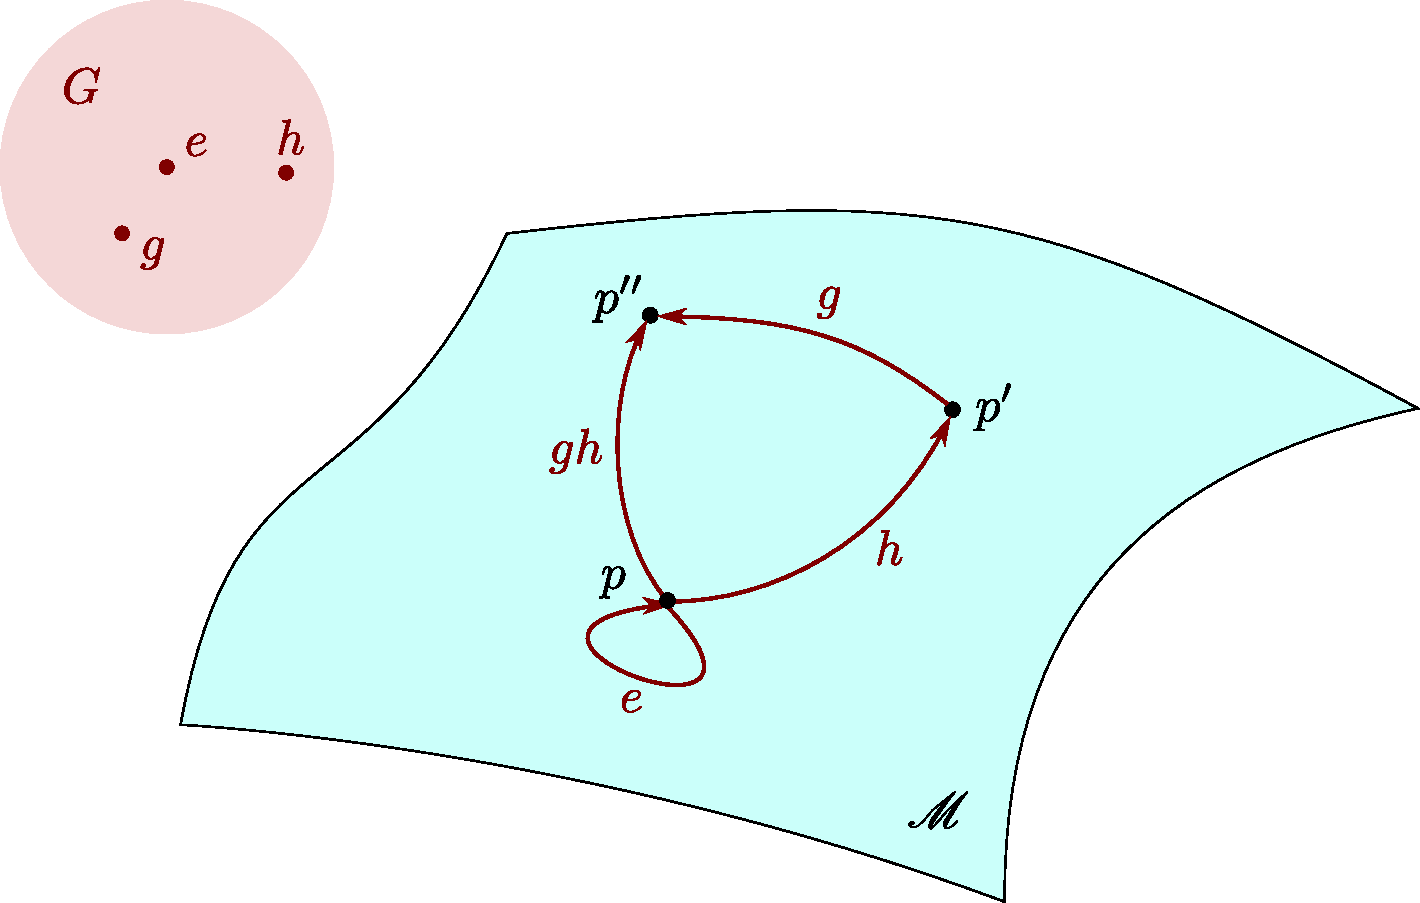
\includegraphics[width=0.8\textwidth]{def_group_action.pdf}}
\caption[]{\label{f:neh:group_action} \footnotesize
Group action of $G$ on $\M$.}
\end{figure}


\subsection{Spacetime symmetries} \label{s:neh:symmetries}

Symmetries of spacetime are described in a coordinate-independent way by means of
a (symmetry) group acting on the spacetime manifold $\M$.
Through this action, each transformation belonging to the group displaces points within $\M$ and one demands that the metric $\w{g}$ is invariant under such displacement.
More precisely, given
a group $G$, a \defin{group action}\index{group!action} of $G$ on $\M$ is a map\footnote{Do no confuse the generic element $g$ of group $G$ with the metric tensor $\w{g}$.}
\be
    \begin{array}{rccl}
    \Phi: & G\times \M & \longrightarrow & \M \\
        & (g,p) & \longmapsto & \Phi(g,p) =: \Phi_g(p)
    \end{array}
\ee
such that (cf. Fig.~\ref{f:neh:group_action})
\begin{itemize}
\item $\forall p\in \M,\  \Phi_e(p) = p$, where $e$ is the identity element of $G$;
\item $\forall (g,h) \in G^2,\  \forall p\in\M,\  \Phi_g(\Phi_h(p)) = \Phi_{gh}(p)$, where $gh$ stands for the product of $g$ by $h$ according to $G$'s group law.
\end{itemize}
The \defin{orbit}\index{orbit!under a group action} of a point $p\in\M$ is the set $\{g(p),\ g\in G\}\subset\M$, i.e. the set of points which are connected to $p$ by some group transformation. One says that $p$ is a
\defin{fixed point}\index{fixed!point} of the group action if its orbit is
reduced to $\{p\}$.

An important class of group actions are those for which $G$ is a 1-dimensional
\emph{Lie group}, i.e. a ``continuous'' group (actually a ``differentiable'' group).
Then around $e$, the elements of $G$ can be labelled by a parameter $t\in \R$, such that $g_{t=0} = e$. It is then
common to use the shorthand notation
\be
        \Phi_t := \Phi_{g_t} .
\ee
Because $G$ is a 1-dimensional Lie group, the orbit of a given point $p\in\M$ under the group action is then either $\{p\}$ (when $p$ is fixed point of the
group action) or a curve of $\M$. In the latter case,
$t$ is a natural parameter along the curve (cf. Fig.~\ref{f:neh:orbit_group}). The tangent vector corresponding to that parameter is called the \defin{generator of the group} $G$
(associated with the $t$-parametrization). At each point $p$ of
an orbit, it is given by
\be \label{e:neh:xi_dxdt}
    \w{\xi} = \frac{\D\w{x}}{\D t} ,
\ee
where $\D\w{x}$ is the infinitesimal vector connecting the point $p$ to the point
$\Phi_{\D t}(p)$ (cf. Sec.~\ref{s:bas:vectors} and Fig.~\ref{f:neh:orbit_group}).
We have then
\begin{greybox}
The group action limited to infinitesimal transformations of parameter
$\D t$ around the identity ($\D t =0$) amounts to translations by the infinitesimal vector $\D t\, \w{\xi}$.
\end{greybox}

\begin{figure}
\centerline{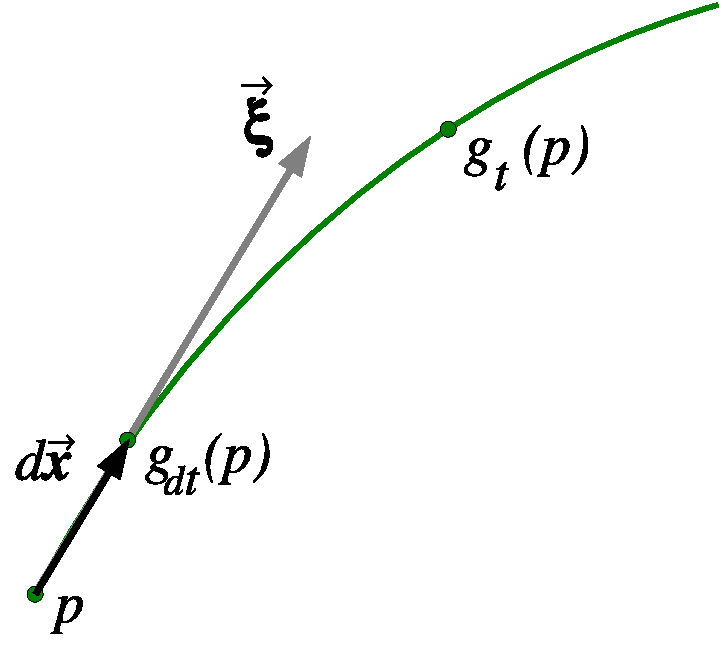
\includegraphics[height=0.25\textheight]{def_orbit_group.pdf}}
\caption[]{\label{f:neh:orbit_group} \footnotesize
Orbit of a point $p$ under the action $\Phi$ of a 1-dimensional Lie group, parametrized
by $t\in\R$. The vector $\w{\xi} = \D\w{x}/\D t$ is the group
generator associated with this parameter.}
\end{figure}

A 1-dimensional Lie group $G$ is said to be a
\defin{symmetry group}\index{symmetry!group}\index{group!symmetry --}
of the spacetime $(\M,\w{g})$ if there is an action $\Phi$ of $G$ on $\M$
such that for any value of the parameter $t$ of $G$,
$\Phi_t$ is an \defin{isometry}\index{isometry} of $(\M,\w{g})$, i.e. $\Phi_t$
preserves the ``distances'' and more generally the ``scalar products'' on
$(\M,\w{g})$, in the following sense: for any $p\in\M$ and any pair of points $(q,r)$
infinitely close to $p$, we shall have
\be \label{e:neh:isometry_dx}
    \left.\w{g}\right| _{\Phi_t(p)}(\D\w{x}', \D\w{y}') =
        \left.\w{g}\right| _{p}(\D\w{x}, \D\w{y}) ,
\ee
with the infinitesimal displacement vectors $\D\w{x} := \vp{pq}$, $\D\w{y} := \vp{pr}$,
$\D\w{x}' := \vp{\Phi_t(p)\Phi_t(q)}$ and $\D\w{y}' := \vp{\Phi_t(p)\Phi_t(r)}$
(cf. Sec.~\ref{s:fra:spacetime}).
Now, by definition, $\D\w{x}'$ is nothing but the pushforward
of the vector $\D\w{x}\in T_p\M$ to the tangent space
$T_{\Phi_t(p)}\M$ by the map $\Phi_t$
(cf. Sec.~\ref{s:bas:Lie_der_vector} of Appendix~\ref{s:bas}),
and similarly $\D\w{y}'$ is the pushforward of $\D\w{y}$ by $\Phi_t$:
\[
    \D\w{x}' = \Phi_t^*(\D\w{x}) \quad\mbox{and}\quad
    \D\w{y}' = \Phi_t^*(\D\w{y}) .
\]
By rescaling by infinitely small parameters (using the bilinearity of $\w{g}$),
it is clear that (\ref{e:neh:isometry_dx})
holds for finite vectors as well, so that we may say that $\Phi_t$ is an
isometry of $(\M,\w{g})$ iff
\be \label{e:neh:isometry}
    \forall p\in\M,\  \forall (\w{u},\w{v}) \in (T_p\M)^2,\quad
    \left. \w{g}\right| _{\Phi_t(p)} \left(\Phi_t^*(\w{u}), \Phi_t^*(\w{v})\right) =
    \left. \w{g}\right| _{p} (\w{u},\w{v}) ,
\ee
where $\Phi_t^*(\w{u})$ (resp. $\Phi_t^*(\w{v})$) is the pushforward of the vector $\w{u}\in T_p\M$ (resp. $\w{v}\in T_p\M$)
to the tangent space $T_{\Phi_t(p)}\M$ by $\Phi_t$ [cf. Eq.~(\ref{e:bas:def_Phi_eps})].
Given the definition (\ref{e:bas:def_pullback}) of the pullback of
a bilinear form, we may reexpress the isometry condition (\ref{e:neh:isometry})
in terms of the
pullback of $\w{g}$ by $\Phi_t$:
\be \label{e:neh:isometry_pullback}
    \Phi_t^*\w{g} = \w{g} .
\ee
According the definition (\ref{e:bas:def_Lie_der_covar}) of the Lie
derivative, we have
\be
    \Lie{\xi} \w{g} := \lim_{t \rightarrow 0} \frac{1}{t}
    \left( \Phi_t^*\w{g} - \w{g} \right) .
\ee
If $G$ is a symmetry group of $(\M,\w{g})$ with generator $\w{\xi}$,
the isometry condition
(\ref{e:neh:isometry_pullback}) leads then to
$\Lie{\xi}\w{g} = 0$. The reverse is true by integration. Hence
we conclude:
\begin{greybox}
A 1-dimensional Lie group $G$
is a symmetry group of the spacetime $(\M,\w{g})$ iff the Lie derivative
of the metric tensor along a generator $\w{\xi}$ of $G$
vanishes identically:
\be \label{e:neh:Lie_xi_g}
    \encadre{\Lie{\xi}\w{g} = 0 } .
\ee
The vector field $\w{\xi}$ is then called a \defin{Killing vector}\index{Killing!vector field}
of $(\M,\w{g})$.
\end{greybox}
Expressing the Lie derivative via Eq.~(\ref{e:bas:Lie_der_comp_nab}) of Appendix~\ref{s:bas},
we see immediately that Eq.~(\ref{e:neh:Lie_xi_g}) is equivalent to the so-called
\defin{Killing equation}\index{Killing!equation}:
\be \label{e:neh:Killing_equation}
    \encadre{ \nabla_\alpha \xi_\beta + \nabla_\beta \xi_\alpha = 0 }.
\ee

If terms of the components $g_{\alpha\beta}$ of $\w{g}$ with respect to
coordinates $(x^\alpha) = (t,x^1,\ldots,x^{n-1})$ adapted to the Killing vector $\w{\xi}$,
i.e. such that $\w{\xi} = \wpar_t$, the isometry condition (\ref{e:neh:Lie_xi_g})
is equivalent to
\be
    \der{g_{\alpha\beta}}{t} = 0 .
\ee
\begin{proof}
This is a direct consequence of the identity (\ref{e:bas:Lie_adapted}).
\end{proof}


\subsection{Definition and examples of Killing horizons} \label{s:neh:def_Killing_hor}

\begin{greybox}
A \defin{Killing horizon}\index{Killing!horizon}\index{horizon!Killing --} is
a null hypersurface $\Hor$ in a spacetime $(\M,\w{g})$ admitting a
Killing vector field $\w{\xi}$ such that, on $\Hor$, $\w{\xi}$ is
normal to $\Hor$.
\end{greybox}

Thus the existence of a Killing horizon requires that the spacetime $(\M,\w{g})$ has
some continuous symmetry
(usually stationarity), namely that it is invariant under the action of a
1-parameter group, as described in Sec.~\ref{s:neh:symmetries}.
A definition equivalent to the above one is then:
\begin{greybox}
A \defin{Killing horizon} is a null
hypersurface $\Hor$ whose null geodesic generators are orbits of a
1-parameter group of isometries of $(\M,\w{g})$.
\end{greybox}

\begin{remark}
The above definition implies that the Killing vector field $\w{\xi}$ is null
and non-vanishing on $\Hor$:
\be \label{s:neh:xi_on_KH}
    \left. \w{\xi}\cdot\w{\xi} \right| _{\Hor} = 0 \qquad\mbox{and}\qquad
    \left. \w{\xi} \right| _{\Hor} \not= 0 .
\ee
Indeed, if $\w{\xi}$ is vanishing at some point of $\Hor$, it cannot be
considered as a normal vector to $\Hor$.
\end{remark}

We shall see in Chap.~\ref{s:sta} that in a stationary spacetime, a black hole
event horizon must be a Killing horizon.

\begin{figure}
\centerline{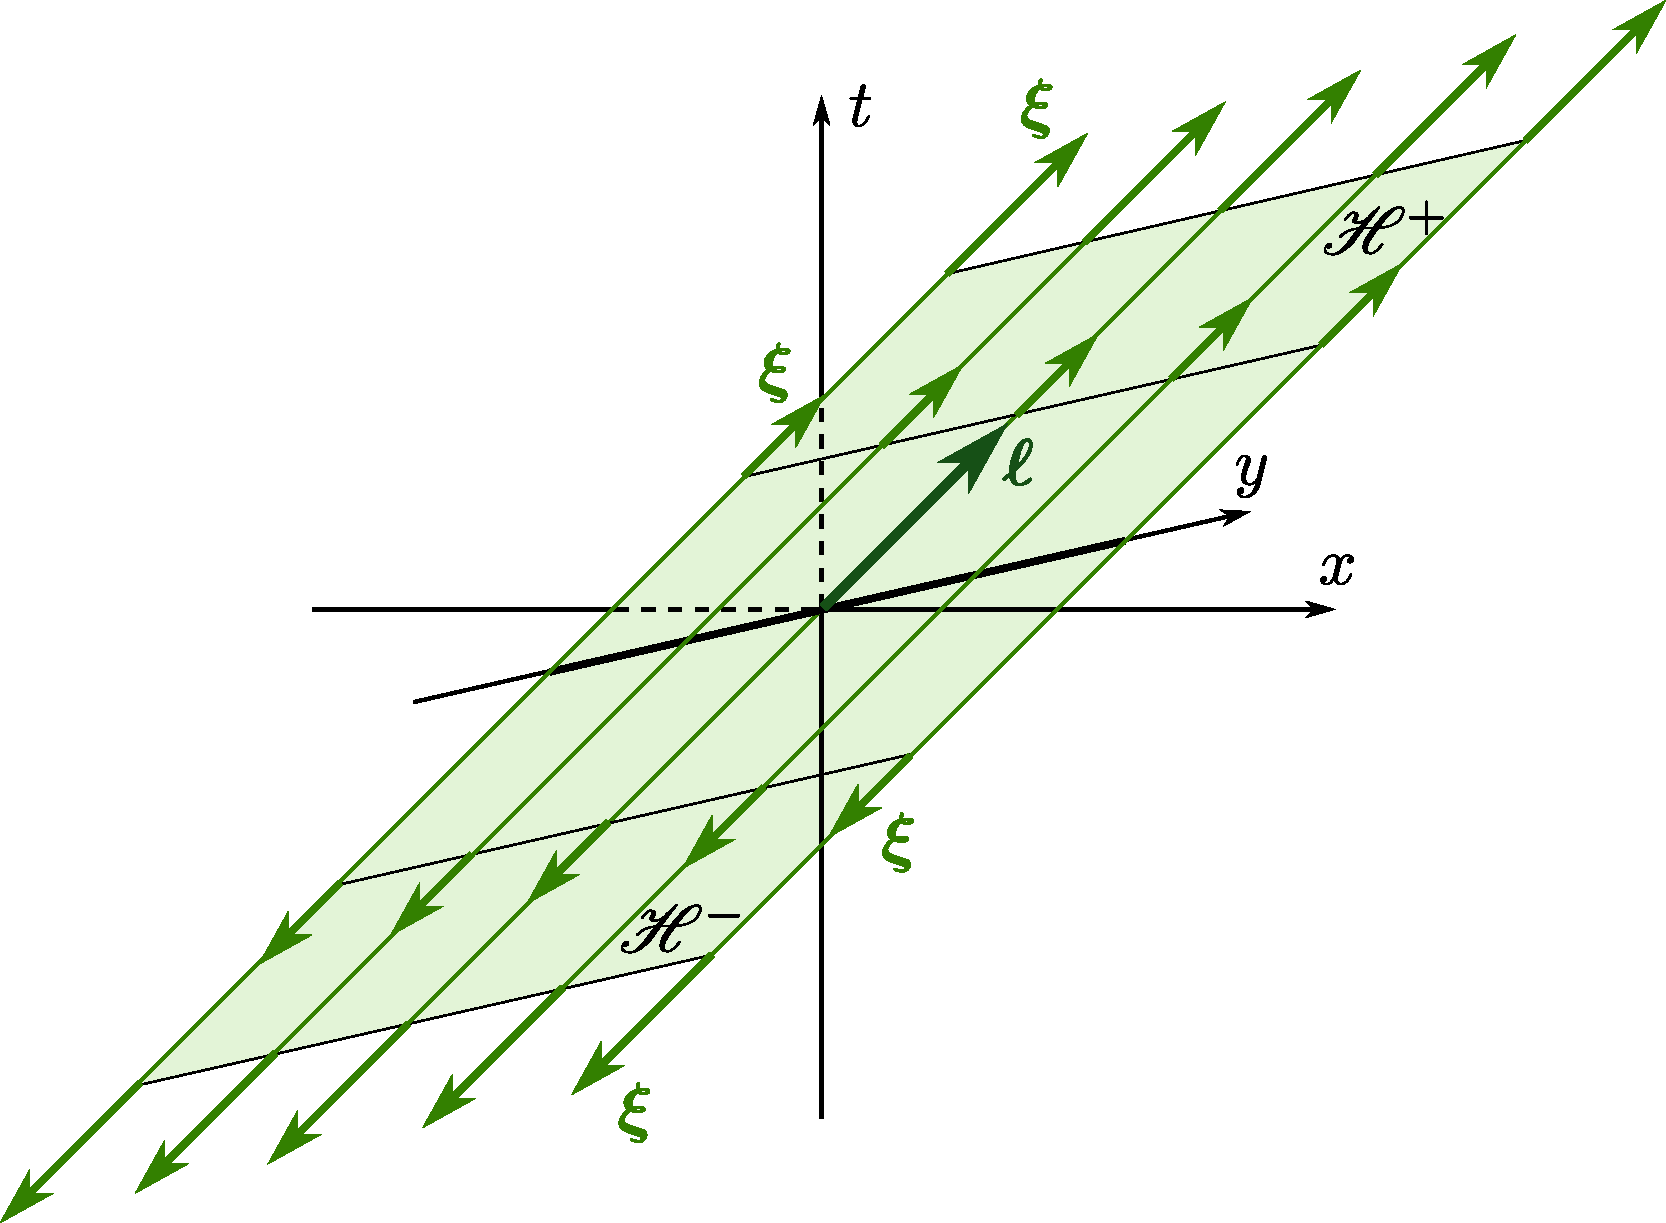
\includegraphics[width=0.6\textwidth]{def_hplaneKilling-boost.pdf}}
\caption[]{\label{f:neh:hplaneKilling-boost} \footnotesize
Null half-hyperplanes $\Hor^+$ and $\Hor^-$ as Killing horizons for the
Killing vector field $\w{\xi}=x \wpar_t + t \wpar_x$ generating Lorentz boosts
in Minkowski spacetime. The green lines are the null geodesic generators of
$\Hor$, while the thick black line (actually a 2-plane) marks the location
where $\w{\xi}$ vanishes.}
\end{figure}

\begin{example}[null hyperplane as a translation-Killing horizon]
\label{x:neh:transKH}
Let us consider the null hyperplane of Minkowski spacetime $\Hor$ discussed in
Examples~\ref{x:def:null_hyp}, \ref{x:def:null_hyp2} and \ref{x:def:null_hyp3}
of Chap.~\ref{s:def}.
$\Hor$ is defined by the equation $t=x$. The vector field
\be
    \w{\xi} := \wpar_t + \wpar_x
\ee
is a Killing vector of Minkowski spacetime: $\w{\xi}$ is the generator of
translations in the direction $\wpar_t + \wpar_x$, and these translations constitute a
1-dimensional subgroup of the Poincaré group --- the symmetry group of Minkowski
spacetime. We note that $\w{\xi}$ coincides with the null vector $\wl$
defined by Eq.~(\ref{e:def:wl_null_hyperplane}). Since $\wl$ is
normal to $\Hor$, we conclude immediately that $\Hor$ is a Killing horizon
with respect to $\w{\xi}$.
\end{example}

\begin{example}[null hyperplane as a boost-Killing horizon]
\label{x:neh:boostKH}
Let us consider the same null hyperplane $\Hor$ as above, but
with another Killing vector of Minkowski spacetime:
\be \label{e:neh:boost-Killing}
    \w{\xi} := x \wpar_t + t \wpar_x .
\ee
This vector is indeed the
generator of the 1-parameter group of Lorentz boosts\index{boost} in the $(t,x)$ plane.
On $\Hor$ we have (cf. Fig.~\ref{f:neh:hplaneKilling-boost}):
\[
    \w{\xi} \equalH t (\wpar_t + \wpar_x) \equalH t \, \wl ,
\]
where $\wl$ is the null normal to $\Hor$ defined by
Eq.~(\ref{e:def:wl_null_hyperplane}) and the notation $\equalH$ means that the equality holds only on $\Hor$. We conclude that $\w{\xi}$ is a normal to
the null hypersurface $\Hor$ as soon as $t\not=0$. Therefore, we may split
$\Hor\setminus\{t=0\}$ in two open half-hyperplanes:
\be \label{e:neh:boost-Killing_hor}
    \Hor^+ := \{ p\in\Hor,\quad t(p) > 0 \} \quad\mbox{and}\quad
    \Hor^- := \{ p\in\Hor,\quad t(p) < 0 \} ,
\ee
so that each of them is a Killing horizon with
respect to $\w{\xi}$ (cf. Fig.~\ref{f:neh:hplaneKilling-boost}).
\end{example}

\begin{example}[null hyperplane as a null-rotation-Killing horizon]
\label{x:neh:nullrotKH}
Another example of Killing horizon is still provided by the null hyperplane
$\Hor$ considered above, but this time with the Killing vector
\be \label{e:neh:xi_null_rotation}
   \w{\xi} := y( \wpar_t + \wpar_x ) + (t-x)\wpar_y .
\ee
This vector is indeed the generator of
null rotations leaving the plane
$\mathrm{Span}(\wl,\wpar_z)$ strictly invariant (cf. e.g. Sec.~6.4.5 of
Ref.~\cite{Gourg13}), $\wl$ being the null normal of $\Hor$ defined by
Eq.~(\ref{e:def:wl_null_hyperplane}). These null rotations form a
1-dimensional subgroup of the Lorentz group, and thereby
a symmetry group of Minkowski spacetime. It is also immediate to check that
the vector defined by (\ref{e:neh:xi_null_rotation}) obeys
Killing equation (\ref{e:neh:Killing_equation}).
On $\Hor$, $t-x=0$, so that
(\ref{e:neh:xi_null_rotation}) reduces to
\[
    \w{\xi}  \equalH y ( \wpar_t + \wpar_x )  \equalH y \, \wl .
\]
It follows that $\w{\xi}$ is a null normal to $\Hor$ as soon as $y\not=0$.
We may then split $\Hor\setminus\{y=0\}$ in two open half-hyperplanes:
\[
    \Hor_1 := \{ p\in\Hor,\quad y(p) < 0 \} \quad\mbox{and}\quad
    \Hor_2 := \{ p\in\Hor,\quad y(p) > 0 \} ,
\]
each of them being a Killing horizon with
respect to $\w{\xi}$ (cf. Fig.~\ref{f:neh:hplaneKilling-nullrot}).
\end{example}

\begin{figure}
\centerline{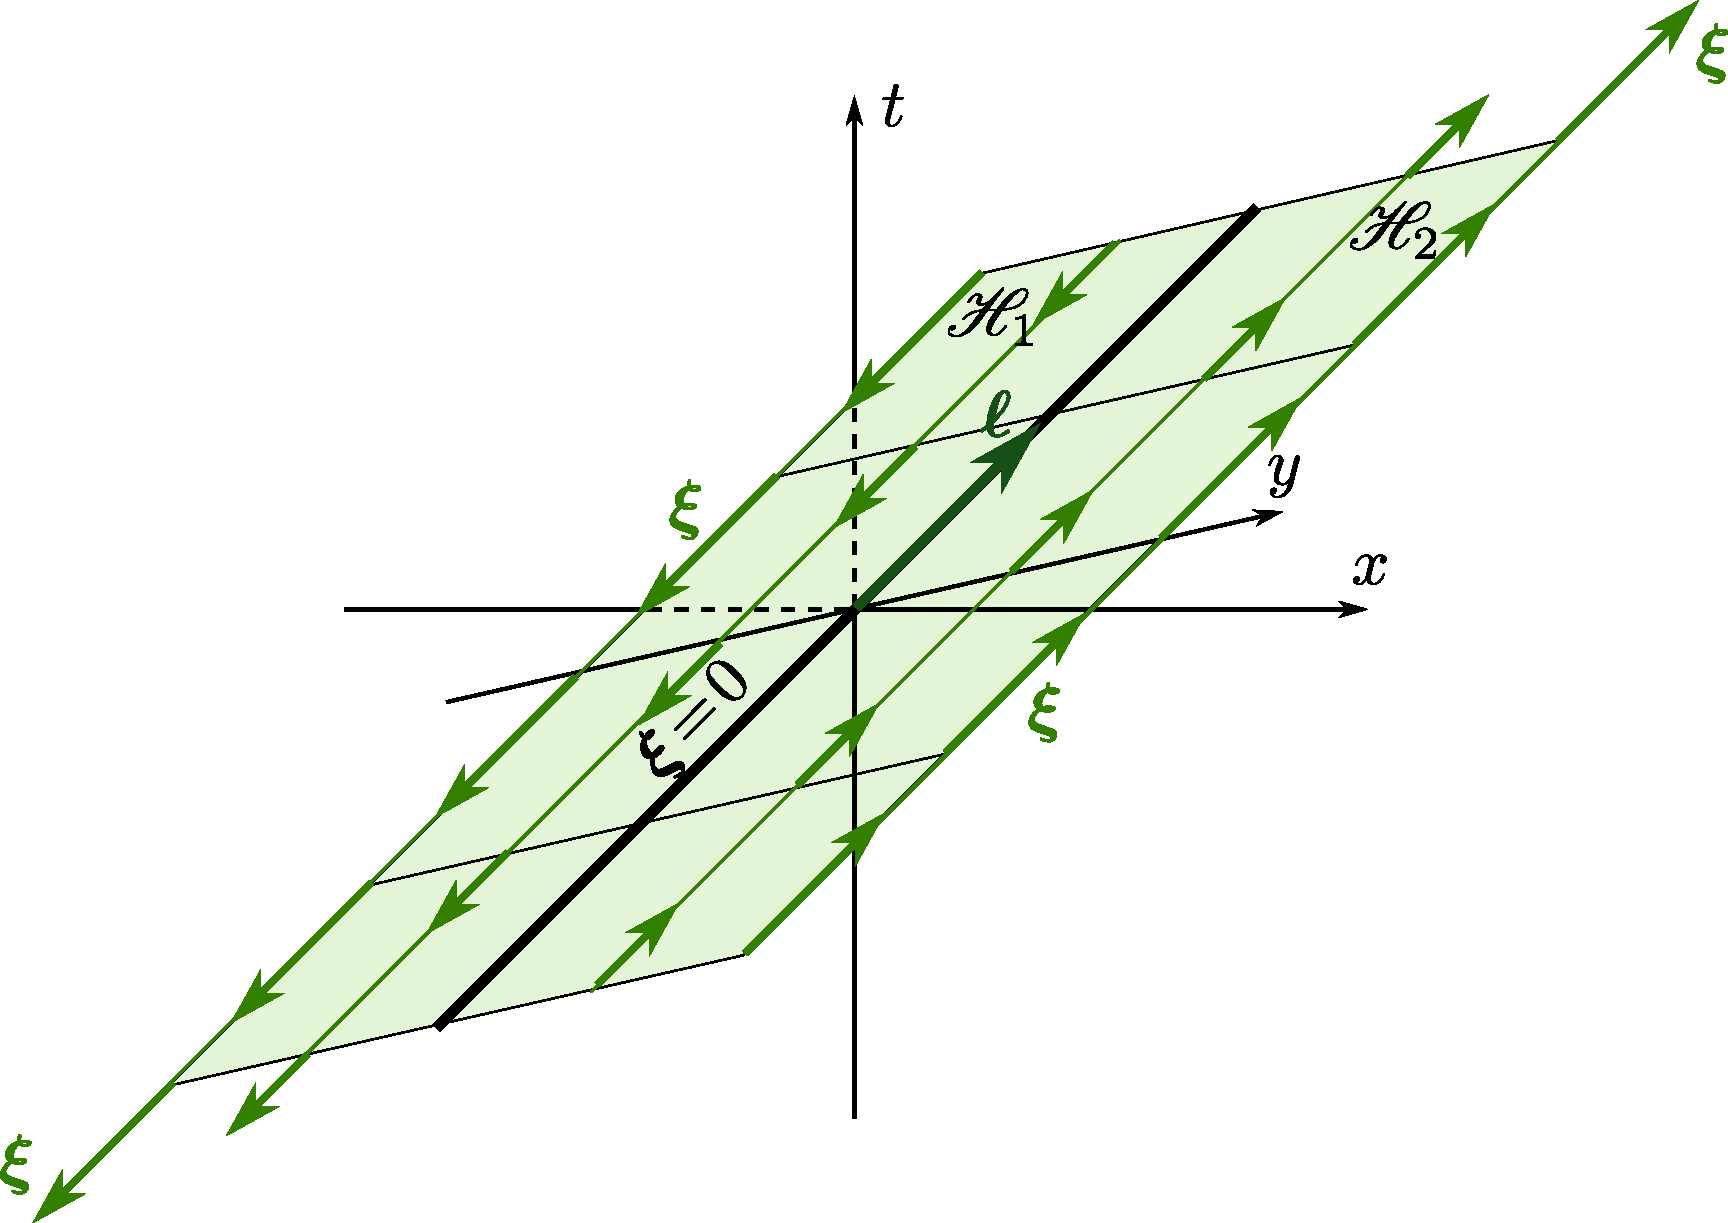
\includegraphics[width=0.6\textwidth]{def_hplaneKilling-nullrot.pdf}}
\caption[]{\label{f:neh:hplaneKilling-nullrot} \footnotesize
Null half-hyperplanes $\Hor_1$ and $\Hor_2$ as Killing horizons for the
Killing vector field $\w{\xi}=y( \wpar_t + \wpar_x ) + (t-x)\wpar_y$
generating null rotations
in Minkowski spacetime. The green lines are the null geodesic generators of
$\Hor$, while the thick black line (actually a 2-plane) marks the location
where $\w{\xi}$ vanishes.}
\end{figure}

\begin{example}[light cone as a counter-example]
The future light cone introduced in Example~\ref{x:def:light_cone} of Chap.~\ref{s:def} is \emph{not} a
Killing horizon of Minkowski spacetime: it is invariant under the action
of the Lorentz group, but its null generators are not invariant
under the action of a single 1-dimensional subgroup of the Lorentz group.
Actually the future light cone is an example of a more general structure,
which Carter has termed a
\defin{local isometry horizon}\index{local!isometry horizon}\index{isometry!horizon}\index{horizon!local isometry --} \cite{Carte67,Carte69}: a null hypersurface that is invariant under
some group $G$ of isometries (here: the Lorentz group) and such that each null
geodesic generator is an orbit of some 1-dimensional subgroup of $G$,
this subgroup being not necessarily the same from one null generator to the next
(here: using Minkowskian spherical
coordinates $(t,r,\th,\ph)$,
the null geodesic generator through the point of coordinates $(1,1,\th_0,\ph_0)$
is the orbit of this point under the subgroup of boosts in the plane
$(\th,\ph) = (\th_0,\ph_0)$). A Killing horizon is a local isometry horizon
for which $\dim G = 1$.
\end{example}


\begin{example}[Schwarzschild horizon] \label{x:neh:Schwarz_KH}
Given the expression (\ref{e:def:wl_Schw_hor}) for the null normal $\wl$
of the family of hypersurfaces $\Hor_u$ and the fact that the Schwarzschild
horizon $\Hor$ is defined by $r=2m$, we have
\be \label{e:neh:wl_wpt_Schw_hor}
    \wl \equalH \wpar_t .
\ee
Now the vector field $\wpar_t$ is clearly a Killing vector of metric $\w{g}$
as given by (\ref{e:def:Schw_metric}), since none of the metric components
$g_{\alpha\beta}$ depends upon $t$. Hence (\ref{e:neh:wl_wpt_Schw_hor})
shows that the Schwarzschild horizon is a Killing horizon. By the way,
Eq.~(\ref{e:neh:wl_wpt_Schw_hor}) was our motivation for the choice of the
null normal $\wl$ performed in Example~\ref{x:def:Schw_hor2} of Chap.~\ref{s:def}.
\end{example}

\begin{hist}
The concept of Killing horizon has been introduced by Brandon Carter\index{Carter, B.} in
1966 \cite{Carte66,Carte67} and developed in an article published in
1969 \cite{Carte69}. The properties of Killing horizons have been
studied in detail by Robert H. Boyer\index{Boyer, R.H.},
in an article prepared posthumously from his notes
by J.~Ehlers and J.L.~Stachel and published in 1969 \cite{Boyer69},
leading to the concept of \emph{bifurcate Killing horizon}, to be discussed in
Sec.~\ref{s:sta:bifur_Killing_hor} (cf. the historical note on page~\pageref{h:sta:Boyer}).
\end{hist}

\subsection{Killing horizons as non-expanding horizons}

Let $\Hor$ be a Killing horizon with cross-sections that are closed manifolds,
i.e. the topology of $\Hor$ is (\ref{e:def:H_topology}). Let us select the null normal $\wl$
that coincides with the Killing vector $\w{\xi}$ on $\Hor$:
$\wl \equalH \w{\xi}$.
Equation~(\ref{e:neh:Lie_xi_g}) then implies:
\[
    \Lie{\el} \w{g} \equalH 0 .
\]
Let $\Sp$ be a cross-section of $\Hor$; since $\w{q}$ is the metric induced by $\w{g}$
on $\Sp$, we deduce immediately that
\[
    \Lie{\el} \w{q} = 0 .
\]
From the definition (\ref{e:def:Theta}), it follows that the expansion rate
tensor of $\Sp$ vanishes identically:
\be \label{e:neh:Theta_zero_KillingH}
    \w{\Theta} = 0 .
\ee
In particular we have
\[
    \theta_{(\wl)} = 0 .
\]
We conclude that
\begin{greybox}
Any Killing horizon with closed-manifold cross-sections is a non-expanding horizon.
\end{greybox}
Moreover, (\ref{e:neh:Theta_zero_KillingH}) shows that $\w{\Theta}$ vanishes
for all Killing horizons, while to get the same result on a generic non-expanding
horizon, one has to assume that the null energy condition holds on $\Hor$.

\subsection{Expressions of the non-affinity coefficient}

Let $\kappa$ be the non-affinity coefficient
(cf. Sec.~\ref{s:def:geod_gener} and \ref{s:geo:gener_param})
of the null normal $\wl$ coinciding with the Killing vector $\w{\xi}$
on a Killing horizon $\Hor$. According to the definition
(\ref{e:def:wl_geod_kappa}), we have
\be
    \wnab_{\w{\xi}}\, \w{\xi} \equalH \kappa \, \w{\xi} .
\ee
The metric dual of this relation is
$\xi^\mu \nabla_\mu \xi_\alpha \equalH \kappa \, \xi_\alpha$.
Using Killing equation (\ref{e:neh:Killing_equation}) under the form
$\nabla_\mu \xi_\alpha = - \nabla_\alpha \xi_\mu$, we get
\[
    \xi^\mu \nabla_\alpha \xi_\mu \equalH - \kappa \, \xi_\alpha .
\]
Now $\xi^\mu \nabla_\alpha \xi_\mu = 1/2 \, \nabla_\alpha (\xi_\mu \xi^\mu)$.
Hence
\be
    \nabla_\alpha (\xi_\mu \xi^\mu) \equalH - 2 \kappa \, \xi_\alpha.
\ee
Since $\xi_\mu \xi^\mu = \w{\xi}\cdot\w{\xi}$ is a scalar field, we may
replace the covariant derivative by the differential:
\be \label{e:neh:dxi2_kappa}
    \encadre{ \dd (\w{\xi}\cdot\w{\xi}) \equalH - 2 \kappa \, \uu{\xi} } .
\ee

Another interesting relation is obtained from the Frobenius relation
(\ref{e:def:ext_der_wl_comp}):
\be \label{e:neh:Frobenius_xi}
  \nabla_\alpha \xi_\beta - \nabla_\beta \xi_\alpha \equalH
  \nabla_\alpha \rho \, \xi_\beta -  \nabla_\beta \rho \, \xi_\alpha  ,
\ee
where $\rho$ is the scalar field defined on $\Hor$ by the hypersurface-orthogonality
condition (\ref{e:def:wl_rho_u}):
\[
    \uu{\xi} \equalH - \mathrm{e}^\rho \, \dd u ,
\]
$u$ being a scalar field such that the equation of $\Hor$ is $u=0$.
Actually, $\rho$ is related to $\kappa$ by Eq.~(\ref{e:def:def_kappa}):
\[
    \kappa = \xi^\mu \nabla_\mu \rho = \wnab_{\w{\xi}}\,  \rho .
\]
Thanks to Killing equation (\ref{e:neh:Killing_equation}), we may reshape
(\ref{e:neh:Frobenius_xi}) to
\[
    2 \nabla_\alpha \xi_\beta \equalH
  \nabla_\alpha \rho \, \xi_\beta -  \nabla_\beta \rho \, \xi_\alpha  .
\]
Taking the square leads to
\bea
    2 \nabla_\mu \xi_\nu \, \nabla^\mu \xi^\nu & \equalH &
        \left( \nabla_\mu \rho \, \xi_\nu -  \nabla_\nu \rho \, \xi_\mu \right)
       \left( \nabla^\mu \rho \, \xi^\nu -  \nabla^\nu \rho \, \xi^\mu \right)
       \nonumber \\
       & \equalH & \nabla_\mu \rho \nabla^\mu \rho
        \underbrace{ \xi_\nu \xi^\nu}_{\equalH 0}
        - \underbrace{\xi^\mu \nabla_\mu \rho}_{\kappa}
         \underbrace{\xi^\nu \nabla_\nu \rho}_{\kappa}
        - \underbrace{\xi^\nu \nabla_\nu \rho}_{\kappa}
            \underbrace{\xi^\mu \nabla_\mu \rho}_{\kappa}
        + \nabla_\nu \rho \nabla^\nu \rho
        \underbrace{ \xi_\mu \xi^\mu}_{\equalH 0}
         \nonumber \\
         & \equalH & - 2 \kappa^2 . \nonumber
\eea
Hence
\be \label{e:neh:kappa2}
    \encadre{\kappa^2 \equalH - \frac{1}{2}
        \nabla_\mu \xi_\nu \nabla^\mu \xi^\nu } .
\ee
This is an explicit expression of $\kappa$ in terms of the Killing vector
field $\w{\xi}$.
However, in actual calculations, it is generally preferable to employ
(\ref{e:neh:dxi2_kappa}) for evaluating $\kappa$, because the latter does not involve
the computation of any covariant derivative, contrary to (\ref{e:neh:kappa2}).


\subsection{The zeroth law of black hole mechanics} \label{s:neh:zeroth_law}

We are going to derive a result of great importance for black hole physics,
namely the non-affinity coefficient $\kappa$ discussed above
is constant on a Killing horizon, provided some mild energy condition holds.

Let us denote by $\wl$ the null normal to $\Hor$ that coincides with
the Killing vector field: $\wl \equalH \w{\xi}$. The vector field
$\wl$ is then a symmetry generator on $\Hor$, which implies
\be
    \Lie{\el} \kappa = 0 .
\ee
This means that $\kappa$ is constant along the field lines of $\wl$ (i.e. the
null geodesic generators of $\Hor$). It could however vary from a field line to another
one. To show that this is not the case, let us consider a cross-section
$\Sp$ of $\Hor$ and project the contracted Ricci identity (\ref{e:def:contract_Ricci_ident})
onto it, via the orthogonal projector $\vw{q}$ introduced in
Sec.~\ref{s:def:spacelike_sections}:
\[
    \nabla_\mu \Theta^\mu_{\ \, \nu} q^\nu_{\ \, \alpha} + \el^\mu \nabla_\mu \omega_\nu q^\nu_{\ \, \alpha}
       - \nabla_\nu \left( \theta_{(\wl)} + \kappa \right) q^\nu_{\ \, \alpha}
        + \left( \theta_{(\wl)} + \kappa \right) \omega_\nu q^\nu_{\ \, \alpha}
        - \Theta_{\alpha\mu} k^\nu \nabla_\nu \el^\mu \nonumber \\
     = R_{\mu\nu} \el^\mu q^\nu_{\ \, \alpha}, \nonumber
\]
where we have used $\Theta_{\nu\mu}  q^\nu_{\ \, \alpha} = \Theta_{\alpha\mu}$
and $\el_\nu q^\nu_{\ \, \alpha} = 0$.
Now, since $\Hor$ is a non-expanding horizon, we may set $\w{\Theta}=0$ and
$\theta_{(\wl)} =0$, so that the above equation reduces to
\be \label{e:neh:zeroth_law_step1}
    \el^\mu \nabla_\mu \omega_\nu q^\nu_{\ \, \alpha} - \nabla_\nu \kappa \, q^\nu_{\ \, \alpha}
    + \kappa  \, \omega_\nu q^\nu_{\ \, \alpha} = R_{\mu\nu} \el^\mu q^\nu_{\ \, \alpha} .
\ee
Let us express $\el^\mu \nabla_\mu \omega_\nu$ in terms of the Lie derivative
of $\w{\omega}$ along $\wl$ via formula (\ref{e:bas:Lie_der_comp_nab}) of Appendix~\ref{s:bas}:
\[
    \Liec{\el}\omega_\nu = \el^\mu \nabla_\mu \omega_\nu + \omega_\mu \nabla_\nu \el^\mu .
\]
Since $\wl$ is a symmetry generator on $\Hor$, we have
\be
    \Lie{\el}\w{\omega} \equalH 0 ,
\ee
so that
\[
    \el^\mu \nabla_\mu \omega_\nu \equalH - \omega_\mu \nabla_\nu \el^\mu .
\]
Accordingly, Eq.~(\ref{e:neh:zeroth_law_step1}) becomes successively
\bea
   & & - \omega_\mu \nabla_\nu \el^\mu  q^\nu_{\ \, \alpha}
     - \nabla_\nu \kappa \, q^\nu_{\ \, \alpha}
    + \kappa  \, \omega_\nu q^\nu_{\ \, \alpha} = R_{\mu\nu} \el^\mu q^\nu_{\ \, \alpha} \nonumber \\
   & &  - \omega_\mu \left(\Theta_\nu^{\ \, \mu}
        + \omega_\nu \el^\mu - \el_\nu k^\sigma \nabla_\sigma \el^\mu \right) q^\nu_{\ \, \alpha}
     - \nabla_\nu \kappa \, q^\nu_{\ \, \alpha}
    + \kappa  \, \omega_\nu q^\nu_{\ \, \alpha} = R_{\mu\nu} \el^\mu q^\nu_{\ \, \alpha} \nonumber \\
   & &   - \omega_\mu
   \underbrace{\Theta_\alpha^{\ \, \mu}}_{0}
        - \underbrace{\omega_\mu \el^\mu}_{\kappa} \omega_\nu q^\nu_{\ \, \alpha}
     - \nabla_\nu \kappa \, q^\nu_{\ \, \alpha}
    + \kappa  \, \omega_\nu q^\nu_{\ \, \alpha} = R_{\mu\nu} \el^\mu q^\nu_{\ \, \alpha}  \nonumber \\
   & &
   - \nabla_\nu \kappa \, q^\nu_{\ \, \alpha} = R_{\mu\nu} \el^\mu q^\nu_{\ \, \alpha} , \nonumber
\eea
where we have used (\ref{e:def:nab_l_Theta}) to get the second line,
the identity
$\el_\nu q^\nu_{\ \, \alpha} = 0$ to get the third one and
(\ref{e:def:omega_l_kappa}) to substitute $\kappa$ for
$\omega_\mu \el^\mu$.
In the above equation appears the covariant derivative of $\kappa$ along $\Sp$,
which we denote by $\DS$:
\be
    \DSc_\alpha \kappa := \nabla_\nu \kappa \, q^\nu_{\ \, \alpha} .
\ee
Using the Einstein equation (\ref{e:fra:Einstein_eq_n}), we may then rewrite
the above relation as
\[
    \DSc_\alpha \kappa = -  \frac{2}{n-2}\,\Lambda\,
    \underbrace{g_{\mu\nu}  \el^\mu q^\nu_{\ \, \alpha}}_{\el^\mu q_{\mu\alpha} = 0}
    - 8\pi \Big( T_{\mu\nu} \el^\mu q^\nu_{\ \, \alpha}
    - \frac{1}{n-2}\,  T \, \underbrace{g_{\mu\nu}  \el^\mu q^\nu_{\ \, \alpha}}_{\el^\mu q_{\mu\alpha} = 0} \Big) ,
\]
i.e.
\be \label{e:neh:DS_kappa_W}
    \DSc_\alpha \kappa = - 8\pi T_{\mu\nu} \el^\mu q^\nu_{\ \, \alpha} .
\ee
To go further, we shall assume that matter and the non-gravitational fields
obey the
\defin{null dominant energy condition}\index{null!dominant energy condition}\index{energy!condition!null dominant--}:
\be
   \begin{array}{ll}
    \w{W} := - \vw{T}(\wl, .) \ & \mbox{is future-directed null or timelike} \\
    & \mbox{for any future-directed null vector $\wl$} .
    \end{array}
\ee
In the above equation, $\vw{T}(\wl, .)$ stands for the vector field
that is the metric dual of the 1-form $\w{T}(\wl, .)$; in index notation,
\[
    W^\alpha = - g^{\alpha\nu} T_{\mu\nu}\el^\mu = - T_\mu^{\ \, \alpha} \el^\mu .
\]
Note that the null dominant energy condition implies the null energy condition
discussed in Sec.~\ref{s:neh:NEH_Theta_zero}, since
\[
    \w{T}(\wl, \wl) = - \w{W}\cdot\wl \geq 0 ,
\]
the inequality holding because both $\w{W}$ and $\wl$ are future-directed.

The null dominant energy condition is implied by continuity by the
\defin{dominant energy condition}\index{dominant energy condition}\index{energy!condition!dominant--}:
\be
   \begin{array}{ll}
    \w{W} := - \vw{T}(\w{u}, .) \ & \mbox{is future-directed null or timelike} \\
    & \mbox{for any future-directed timelike vector $\w{u}$} .
    \end{array}
\ee
Physically, the dominant energy condition states that, with respect to any
observer (represented by its 4-velocity $\w{u}$, which is future-directed timelike),
the energy of matter and non-gravitational fields, moves at a speed
at most equal to $c$.

We note that in the right-hand side of (\ref{e:neh:DS_kappa_W}), there appears the
orthogonal projection of $\w{W}$ onto $\Sp$ (more precisely its metric dual).
If we assume the null dominant energy condition, the null energy condition
holds and we have, according to (\ref{e:neh:T_l_l_zero}),
\[
    \wl \cdot \w{W} = - \w{T}(\wl, \wl) = 0 ,
\]
This implies that the vector $\w{W}$ is tangent to $\Hor$. The latter
being a null hypersurface, $\w{W}$ must then be
either collinear to $\wl$ or spacelike (cf. the lemma in Sec.~\ref{s:def:spacelike_sections}).
Now, according to the null dominant energy condition, $\w{W}$ cannot be
spacelike. We conclude that $\w{W}$ is collinear to $\wl$. Consequently its
orthogonal projection onto $\Sp$ is zero:
\[
    q^\alpha_{\ \, \nu} W^\nu = - q^\alpha_{\ \, \nu} T_\mu^{\ \, \nu} \el^\mu = 0 .
\]
Hence the right-hand side of (\ref{e:neh:DS_kappa_W}) vanishes identically
and we are left with
\[
    \DSc_\alpha \kappa = 0 .
\]
This means that $\kappa$ is constant over $\Sp$. Given that $\kappa$ is
constant along each null geodesic generator of $\Hor$, this completes the demonstration
that $\kappa$ is constant over $\Hor$. More precisely, we have shown that
\begin{greybox}
If matter and non-gravitational fields obey the dominant energy condition
on the Killing horizon $\Hor$, then the non-affinity coefficient $\kappa$
of the null normal coinciding with the Killing vector field on
$\Hor$ is constant over $\Hor$:
\be \label{e:neh:zeroth_law}
    \encadre{\kappa = \mathrm{const}.}
\ee
\end{greybox}
In the context of Killing horizons, the non-affinity coefficient $\kappa$ is
called the horizon's \defin{surface gravity}\index{surface!gravity},
for a reason to be detailed in Sec.~\ref{s:neh:surface_gravity},
and the result
(\ref{e:neh:zeroth_law}) is known as the
\defin{zeroth law of black hole mechanics}\index{zeroth law}. More precisely,
the latter states that the surface gravity of a black hole in equilibrium is
constant and we shall see in Chap.~\ref{s:sta} that the event horizon of a black hole in
equilibrium is a Killing horizon.

\begin{example}[null hyperplane as a translation-Killing horizon]
\label{x:neh:transKH_kappa}
For the null hyperplane $\Hor$ considered in Example~\ref{x:neh:transKH} as a Killing horizon with respect to the translation group along its normal, we have
$\kappa = 0$, as already noticed in Example~\ref{x:def:null_hyp3} of Chap.~\ref{s:def}
[Eq.~(\ref{e:def:kappa_0_nullhyp})], which is obviously constant over $\Hor$.
\end{example}

\begin{example}[null hyperplane as a boost-Killing horizon]
\label{x:neh:boostKH_kappa}
Let us consider each of the null half-hyperplanes $\Hor^+$
and $\Hor^-$ of Example~\ref{x:neh:boostKH}, which are Killing horizons with
respect to the boost Killing vector $\w{\xi} = x \wpar_t + t \wpar_x$. On
$\Hor^+$, the future-directed null normal coinciding with this Killing vector
is $\wl^+ = t\,  \wl$, $\wl$ being the geodesic null normal defined by
$\wl:= \wpar_t + \wpar_x$ [cf. Eq.~(\ref{e:def:wl_null_hyperplane})].
Using $\kappa_{\wl} = 0$ and the scaling law (\ref{e:def:rescale_kappa}),
we get the non-affinity
coefficient of $\wl^+$ as $\kappa_+= \wnab_{\wl} t = \partial_t t + \partial_x t$, i.e.
\[
    \kappa_+ = 1 .
\]
On $\Hor^-$, $\w{\xi}$ is past-directed (cf. Fig.~\ref{f:neh:hplaneKilling-boost}).
Sticking to future-directed null normals, we shall then consider $\Hor^-$
as a Killing horizon with respect to the Killing vector field $-\w{\xi}$.
The future-directed null normal coinciding with $-\w{\xi}$ on $\Hor^-$ is then
$\wl^- = -t\,  \wl$, from which we deduce the non-affinity
coefficient of $\wl^-$: $\kappa_-= \wnab_{\wl} (-t) = \partial_t (-t) + \partial_x (-t)$, i.e.
\[
    \kappa_- = -1 .
\]
We check that $\kappa_+$ (resp.  $\kappa_-$) is constant over the Killing horizon $\Hor^+$ (resp. $\Hor^-$), in agreement with the result above.
\end{example}

\begin{example}[null hyperplane as a null-rotation-Killing horizon]
\label{x:neh:nullrotKH_kappa}
In Example~\ref{x:neh:nullrotKH}, we have introduced the Killing horizons
$\Hor_1$ and $\Hor_2$ with respect to the null-rotation Killing vector
$\w{\xi} = y( \wpar_t + \wpar_x ) + (t-x)\wpar_y$ of Minkowski spacetime.
On $\Hor_1$, $\w{\xi}$ is past-directed (cf. Fig.~\ref{f:neh:hplaneKilling-nullrot}),
so that we shall actually consider $\Hor_1$
as a Killing horizon with respect to the Killing vector field $-\w{\xi}$.
The future-directed null normal coinciding with $-\w{\xi}$ on $\Hor_1$ is then
$\wl_1 = - y\, \wl$. Since it is clearly constant along the null geodesic generators
of $\Hor_1$, we have $\wnab_{\wl_1}\wl_1 = 0$, hence the
associated non-affinity coefficient vanishes:
\[
    \kappa_1 = 0 .
\]
On $\Hor_2$, $\w{\xi}$ is future-directed (cf. Fig.~\ref{f:neh:hplaneKilling-nullrot})
and the null normal coinciding with it is $\wl_2 =  y\,  \wl$, whose non-affinity
coefficient is
\[
    \kappa_2 = 0 .
\]
\end{example}

\begin{example}[Schwarzschild and Kerr horizons]
\label{x:neh:Schw_Kerr_kappa}
We have found in Example~\ref{x:def:Schw_hor3} of Chap.~\ref{s:def} [cf. Eq.~(\ref{e:def:kappa_Schw_hor})]
that on a Schwarzschild horizon:
\[
  \kappa = \frac{1}{4m},
\]
which is clearly constant. But
this last feature is rather trivial since the Schwarzschild horizon is spherically
symmetric, so that no dependence of $\kappa$ on $\th$ nor $\ph$ could have been expected.
A much less trivial example is that of the event horizon of a Kerr black hole,
which we shall discuss in Chap.~\ref{s:ker}. This horizon is only axisymmetric,
so that a priori $\kappa$ could depend on $\th$. But it does not, as we shall
see in Sec.~\ref{s:ker:surf_grav}:
\[
    \kappa = \frac{\sqrt{m^2 - a^2}}{2m(m + \sqrt{m^2-a^2})} ,
\]
where $(m,a)$ are the two constant parameters of the Kerr solution. Note that for $a=0$,
we recover the Schwarzschild value: $\kappa= 1/(4m)$.
\end{example}

\begin{hist}
The constancy of $\kappa$ for a Killing horizon has been proven by Stephen Hawking\index{Hawking, S.W.}
in his lecture at the famous Les Houches School of Summer 1972 \cite{Hawki73} (p.~43).
It has also been proven without requiring the dominant energy condition, but
assuming axisymmetry by Brandon Carter\index{Carter, B.} in his lecture at the same Les Houches School
\cite{Carte73b} (Theorem 8, p.~167).
A third proof of the constancy of $\kappa$ using the dominant energy condition
has also been given in 1973 by James Bardeen\index{Bardeen, J.M.}, Brandon Carter and
Stephen Hawking
in their seminal article \emph{The Four Laws of Black Hole Mechanics}
\cite{BardeCH73}.
\end{hist}

\subsection{Classification of Killing horizons} \label{s:neh:classif_KH}

Since $\kappa$ is constant on $\Hor$ (assuming the dominant
energy condition), we may use it to classify Killing horizons in two
categories, depending whether $\kappa$ vanishes or not:
\begin{itemize}
\item if $\kappa = 0$, the Killing vector $\w{\xi}$ is then a geodesic vector on $\Hor$
and $\Hor$ is called a \defin{degenerate Killing horizon}\index{degenerate!Killing horizon}\index{Killing!horizon!degenerate --};
\item if $\kappa \not=0$, $\w{\xi}$ is only a pregeodesic vector on $\Hor$
(cf. Sec.~\ref{s:geo:gener_param})
and $\Hor$ is called a \defin{non-degenerate Killing horizon}\index{non-degenerate!Killing horizon}\index{Killing!horizon!non-degenerate --}.
\end{itemize}

\begin{example}
In Minkowski spacetime, the null hyperplane as a translation-Killing horizon
(Example~\ref{x:neh:transKH_kappa}) and the two half-hyperplanes as
null-rotation-Killing horizons (Example~\ref{x:neh:nullrotKH_kappa}) are
degenerate Killing horizons, while the two half-hyperplanes as
boost-Killing horizons (Example~\ref{x:neh:boostKH_kappa}) are non-degenerate.
From the values of $\kappa$ given in Example~\ref{x:neh:Schw_Kerr_kappa},
we see that the Schwarzschild horizon and the Kerr horizon for
$a<m$ are non-degenerate Killing horizons, while the Kerr horizon for
$a=m$ is a degenerate one.
\end{example}

\subsection{Interpretation of $\kappa$ as a ``surface gravity''}
\label{s:neh:surface_gravity}

In this section, we assume that $\Hor$ is a non-degenerate Killing horizon,
i.e. that $\kappa\not=0$.
Let $p\in\Hor$ and $\w{v}\in T_p\M$ be a vector \emph{transverse} to $\Hor$, i.e.
not tangent to $\Hor$. According to Eq.~(\ref{e:neh:dxi2_kappa}), we have
\[
    \wnab_{\w{v}} (\w{\xi}\cdot\w{\xi}) = - 2\kappa \, \w{\xi}\cdot\w{v} .
\]
The right-hand side of this expression does not vanish, because
$\kappa\not=0$ and $\w{\xi}\cdot\w{v} \not=0$ (since $\w{v}$ is not
tangent to $\Hor$). Hence we have
\[
    \wnab_{\w{v}} (\w{\xi}\cdot\w{\xi}) \not= 0 .
\]
In other words, the derivative of the scalar square $\w{\xi}\cdot\w{\xi}$
along any direction transverse to $\Hor$ does not vanish. Since
$\w{\xi}\cdot\w{\xi}=0$ on $\Hor$, we conclude that, in the vicinity of $\Hor$,
$\w{\xi}\cdot\w{\xi}<0$ on one side of $\Hor$ and $\w{\xi}\cdot\w{\xi}>0$ on the
other side:
\begin{greybox}
In the vicinity of a non-degenerate Killing horizon $\Hor$, the Killing vector field $\w{\xi}$ is timelike on one side of $\Hor$, null on $\Hor$
and spacelike on the other side.
\end{greybox}

Let us focus on the region in the vicinity of $\Hor$ where $\w{\xi}$ is timelike.
There we define the ``norm'' of $\w{\xi}$ by
\be
   \encadre{ V := \sqrt{-\w{\xi}\cdot\w{\xi}} } .
\ee
We have $V>0$ and the square of the gradient of $V$ provides a new expression
of $\kappa$:
\be  \label{e:neh:kappa2_nabV}
    \encadre{ \kappa^2 = \lim_{\Hor} \nabla_\mu V \nabla^\mu V } ,
\ee
where $\lim_{\Hor}$ stands for the limit as one approaches $\Hor$
from the timelike side, which implies $V\rightarrow 0$.
\begin{proof}
Let us consider the 3-form $\w{\omega}$ defined by
\bea
    \omega_{\alpha\beta\gamma} & := & \xi_{[\alpha}\nabla_\beta\xi_{\gamma]} \nonumber \\
        & = & \frac{1}{6} \left[
        \xi_\alpha \left( \nabla_\beta \xi_\gamma - \nabla_\gamma \xi_\beta \right)
        + \xi_\beta \left( \nabla_\gamma \xi_\alpha - \nabla_\alpha \xi_\gamma \right)
        + \xi_\gamma \left( \nabla_\alpha \xi_\beta - \nabla_\beta \xi_\alpha \right)
        \right] , \label{e:neh:antisym_omega}
\eea
the second line being simply the explicit expression of the full antisymmetrization
of $ \xi_{\alpha}\nabla_\beta\xi_{\gamma}$, which is denoted by square brackets in the first line.
Killing equation (\ref{e:neh:Killing_equation}) enables us to simplify each term inside
parentheses in (\ref{e:neh:antisym_omega}), yielding
\be
    \omega_{\alpha\beta\gamma} = \frac{1}{3} \left(
        \xi_\alpha  \nabla_\beta \xi_\gamma
        + \xi_\beta  \nabla_\gamma \xi_\alpha
        + \xi_\gamma  \nabla_\alpha \xi_\beta \right) .
\ee
The ``square'' of $\w{\omega}$ is then
\bea
     \omega_{\mu\nu\rho} \, \omega^{\mu\nu\rho} & = & \frac{1}{9} \Big(
       \xi_\mu  \nabla_\nu \xi_\rho \, \xi^\mu  \nabla^\nu \xi^\rho
       + \xi_\mu  \nabla_\nu \xi_\rho \, \xi^\nu  \nabla^\rho \xi^\mu
       + \xi_\mu  \nabla_\nu \xi_\rho \, \xi^\rho  \nabla^\mu \xi^\nu
       \nonumber \\
       & & \quad + \xi_\nu  \nabla_\rho \xi_\mu \, \xi^\mu  \nabla^\nu \xi^\rho
       + \xi_\nu  \nabla_\rho \xi_\mu \, \xi^\nu  \nabla^\rho \xi^\mu
       + \xi_\nu  \nabla_\rho \xi_\mu \, \xi^\rho  \nabla^\mu \xi^\nu
       \nonumber \\
       & & \quad + \xi_\rho  \nabla_\mu \xi_\nu \, \xi^\mu  \nabla^\nu \xi^\rho
       + \xi_\rho  \nabla_\mu \xi_\nu \, \xi^\nu  \nabla^\rho \xi^\mu
       + \xi_\rho \nabla_\mu \xi_\nu \, \xi^\rho  \nabla^\mu \xi^\nu  \Big)  . \nonumber
\eea
Now in the first line,
\be \label{e:neh:omega_square1}
  \xi_\mu  \nabla_\nu \xi_\rho \, \xi^\mu  \nabla^\nu \xi^\rho =
    \xi_\mu  \xi^\mu  \nabla_\nu \xi_\rho \nabla^\nu \xi^\rho =
    - V^2 \nabla_\nu \xi_\rho \nabla^\nu \xi^\rho
    = - V^2 \nabla_\mu \xi_\nu \nabla^\mu \xi^\nu
\ee
and (using Killing equation (\ref{e:neh:Killing_equation}))
\be \label{e:neh:omega_square2}
    \xi_\mu  \nabla_\nu \xi_\rho \, \xi^\nu  \nabla^\rho \xi^\mu
        =  \xi_\mu \nabla^\rho \xi^\mu \, \xi^\nu  \nabla_\nu \xi_\rho
        = - \xi_\mu \nabla^\rho \xi^\mu \, \xi^\nu  \nabla_\rho \xi_\nu
        = - \frac{1}{4} \nabla^\rho V^2 \, \nabla_\rho V^2
        = - V^2 \nabla^\rho V \, \nabla_\rho V  .
\ee
Actually, we notice that each line
is made of one term of type (\ref{e:neh:omega_square1})
and two terms of type (\ref{e:neh:omega_square2}). Hence
\be \label{e:neh:omega_square_V}
    \omega_{\mu\nu\rho} \, \omega^{\mu\nu\rho} = - \frac{V^2}{3}
    \left( \nabla_\mu \xi_\nu \nabla^\mu \xi^\nu + 2 \nabla_\mu V \nabla^\mu V \right) .
\ee
On $\Hor$, each of the terms inside parentheses in Eq.~(\ref{e:neh:antisym_omega})
can be expressed thanks to the Frobenius identity (\ref{e:neh:Frobenius_xi}):
\[
    \omega_{\alpha\beta\gamma} \equalH
    \frac{1}{6} \left[
        \xi_\alpha \left( \nabla_\beta \rho\,  \xi_\gamma - \nabla_\gamma \rho \, \xi_\beta \right)
        + \xi_\beta \left( \nabla_\gamma  \rho \, \xi_\alpha - \nabla_\alpha  \rho \, \xi_\gamma \right)
        + \xi_\gamma \left( \nabla_\alpha  \rho \,  \xi_\beta - \nabla_\beta  \rho \, \xi_\alpha \right)
        \right] .
\]
We notice that all terms in the right-hand side canceal two by two, yielding
\be \label{e:neh:omega_abc_zero}
    \omega_{\alpha\beta\gamma} \equalH 0 .
\ee
Equation~(\ref{e:neh:omega_abc_zero}) is actually nothing but
a variant of Frobenius theorem\index{Frobenius!theorem},
expressing the fact that the vector field $\w{\xi}$
is hypersurface-orthogonal on $\Hor$ (see e.g.
Eq.~(B.3.6) in Wald's textbook \cite{Wald84}).
Let us evaluate the gradient of the square
(\ref{e:neh:omega_square_V}) and take the limit
on $\Hor$:
\bea
    \nabla_\alpha \omega_{\mu\nu\rho} \, \underbrace{\omega^{\mu\nu\rho}}_{\to 0}
 + \underbrace{\omega_{\mu\nu\rho}}_{\to 0} \nabla_\alpha  \omega^{\mu\nu\rho} & =&
  - \frac{1}{3} \underbrace{\nabla_\alpha V^2}_{\to 2\kappa \xi_\alpha}
    \Big( \underbrace{\nabla_\mu \xi_\nu \nabla^\mu \xi^\nu}_{\to -2\kappa^2} + 2 \nabla_\mu V \nabla^\mu V \Big)
        \nonumber \\
 &  & -  \frac{1}{3} \underbrace{V^2}_{\to 0}  \nabla_\alpha \left( \nabla_\mu \xi_\nu \nabla^\mu \xi^\nu + 2 \nabla_\mu V \nabla^\mu V \right) ,  \nonumber
\eea
where we have used Eq.~(\ref{e:neh:dxi2_kappa}) in the form $\nabla_\alpha V^2 \equalH 2 \kappa \xi_\alpha$, as well as expression~(\ref{e:neh:kappa2}) of $\kappa^2$. Hence we are left with
\[
    \kappa \left(  \nabla_\mu V \nabla^\mu V - \kappa^2 \right)
     \xi_\alpha \longrightarrow 0 \quad\mbox{on}\ \Hor .
\]
Now, by the very definition of a Killing horizon, $\xi_\alpha \not=0$ on $\Hor$.
Moreover, $\Hor$ being a non-degenerate Killing horizon, we have $\kappa\not=0$ as well.
The above limit is then equivalent to (\ref{e:neh:kappa2_nabV}).
\end{proof}

In the region where $\w{\xi}$ is timelike, the vector field
\be
    \w{u} := \frac{1}{V}\, \w{\xi}
\ee
is a future-directed unit timelike vector field. It is future-directed
because by convention\footnote{Were $\w{\xi}$ past-directed, we could always
consider the Killing field $-\w{\xi}$ instead.} $\w{\xi}$ is future-directed
null on $\Hor$ and by continuity this orientation must be preserved in the
region where $\w{\xi}$ is timelike.
The unit vector field $\w{u}$ can be then considered as the 4-velocity
of an observer $\Obs$, whose worldline of is a field line of $\w{\xi}$,
i.e. an orbit of the isometry group generated by $\w{\xi}$.
One may call $\Obs$ a
\defin{stationary observer}\index{stationary!observer}\index{observer!stationary --}
since the spacetime geometry is not changing along its worldline.
The 4-acceleration of $\Obs$ is
\bea
    \w{a} & := & \wnab_{\w{u}}\, \w{u} \nonumber \\
        & = & \wnab_{V^{-1}\w{\xi}}\, \left( V^{-1} \w{\xi} \right)
        = V^{-1} \wnab_{\w{\xi}}\, \left( V^{-1} \w{\xi} \right)
        = V^{-1} \left[ - V^{-2} (\wnab_{\w{\xi}} V )\, \w{\xi}
            + V^{-1} \wnab_{\w{\xi}}\, \w{\xi} \right] . \nonumber
\eea
Now, since $\w{\xi}$ is a symmetry generator, $\wnab_{\w{\xi}} V =0$. This
can be shown explicitly by means of Killing equation (\ref{e:neh:Killing_equation}):
\[
    \wnab_{\w{\xi}} V = \xi^\mu \nabla_\mu( \sqrt{-\xi_\nu \xi^\nu} )
        = - \frac{1}{2\sqrt{-\xi_\nu \xi^\nu}} \, \xi^\mu \nabla_\mu( \xi_\nu \xi^\nu )
        = -\frac{1}{V}
            \underbrace{\xi^\mu \xi^\nu \nabla_\mu \xi_\nu}_{0}
        = 0 .
\]
We have thus
\be
    \w{a} = \frac{1}{V^2} \, \wnab_{\w{\xi}}\, \w{\xi}  ,
\ee
from which
\[
    a_\alpha = \frac{1}{V^2} \, \xi^\mu \nabla_\mu \xi_\alpha .
\]
Thanks to Killing equation (\ref{e:neh:Killing_equation}), we may rewrite
this relation as
\[
    a_\alpha = - \frac{1}{V^2} \, \xi^\mu \nabla_\alpha \xi_\mu
        = - \frac{1}{2V^2} \, \nabla_\alpha (\xi_\mu \xi^\mu)
        = \frac{1}{2V^2} \, \nabla_\alpha V^2
        = \frac{1}{2}\,  \nabla_\alpha \ln V^2  =  \nabla_\alpha \ln V ,
\]
hence
\be
    \w{a} = \vw{\nabla} \ln V .
\ee
The norm of $\w{a}$, which is always a spacelike vector (since the unit character
of $\w{u}$ implies $\w{u}\cdot\w{a}=0$), is
\be
    a := \sqrt{\w{a}\cdot\w{a}} = \frac{1}{V} \sqrt{\nabla_\mu V \nabla^\mu V} .
\ee
Given the result (\ref{e:neh:kappa2_nabV}), we get an expession of $\kappa$
involving $a$:
\be \label{e:neh:kappa_lim_Va}
    \encadre{ \kappa = \lim_{\Obs\rightarrow\Hor} V a } ,
\ee
where $\Obs\rightarrow\Hor$ means that the limit is achieved by choosing
the worldline of observer $\Obs$ arbitrarily close to $\Hor$.
Since $V \rightarrow 0$ as one approaches $\Hor$, it follows that
\be
     \lim_{\Obs\rightarrow\Hor} a = +\infty .
\ee
This means that the acceleration felt by observer $\Obs$ (the ``gravity'')
diverges as $\Obs$ is placed more and more close to $\Hor$. In that sense,
the \emph{physical} surface gravity of $\Hor$ is infinite. But
Eq.~(\ref{e:neh:kappa_lim_Va}) shows that the rescaled acceleration
$V a$ remains finite as one approaches $\Hor$, and tends to $\kappa$.
It is this quantity that is
named the \defin{surface gravity}\index{surface!gravity}\index{gravity!surface --}
of the Killing horizon $\Hor$.

\begin{remark}
As stressed above, the surface gravity $\kappa$ is not the
actual gravity $a$ measured \emph{locally}, i.e. by an observer at rest with
respect to $\Hor$ and infinitely close to it. However, $\kappa$ can be interpreted
as a physical force (per unit mass) measured by a \emph{distant} observer,
at least in the special case of a Schwarzschild black hole, for which
$\w{\xi}$ is timelike in the entire region outside the Killing horizon\footnote{This is not true for a rotating Kerr black hole:
$\w{\xi}$ becomes null at some ``light-cylinder'' outside $\Hor$ and is then
spacelike away from it, cf. Eq.~(\ref{e:ker:def_chi}),
where $\w{\xi}$ is denoted by $\w{\chi}$.}. In this case, one can identify $\kappa$
to the force exerted by an observer ``at infinity'' to hold in place a particle
of unit mass close to $\Hor$ by means of an infinitely long massless string
(see e.g. Sec.~5.2.4 of Poisson's textbook \cite{Poiss04}).
\end{remark}


%%%%%%%%%%%%%%%%%%%%%%%%%%%%%%%%%%%%%%%%%%%%%%%%%%%%%%%%%%%%%%%%%%%%%%%%%%%%%%%%%%%%%%%%

\section{Summary}

Here is an inheritance diagram summarizing the main results of this chapter.
The vertical arrow means ``is a'', i.e. the element at the bottom of the arrow
is a special case of the element at the top of the arrow.
``NEC'' stands for ``Null Energy Condition''
and ``NDEC'' for ``Null Dominant Energy condition''.

\begin{center}

\begin{tikzpicture}
%\tikzstyle{boxst}=[rectangle,draw]
\tikzstyle{boxst}=[draw, thick, align=center, fill=yellow!20, rounded corners]
\tikzstyle{inherits}=[->,very thick,>=latex]
\node[boxst] (N) at (0,7) {\textbf{Null hypersurface}\\
null geodesic generators\\
$\wnab_{\wl}\wl = \kappa\wl$};
\node[boxst] (H) at (0,3.5) {\textbf{Non-expanding horizon}\\
closed-manifold cross-sections\\
$\theta_{(\wl)}=0$\\
area independent of the cross-section\\
\begin{tabular}{lcl}
NEC &$\Longrightarrow$ & $\w{\Theta}=0$ \\
 & $\Longrightarrow$ & induced affine connection
\end{tabular}
};
\node[boxst] (K) at (0,0) {\textbf{Killing horizon}\\
\textbf{\small with closed-manifold cross-sections}\\
$\w{\Theta}=0$ \\
NDEC $\Longrightarrow \kappa=\mathrm{const}$ (Zeroth Law)};
\draw[inherits] (H)--(N);
\draw[inherits] (K)--(H);
\end{tikzpicture}

\end{center}
  % The concept of black hole 2: Non-expanding horizons

\chapter{The concept of black hole 3: The global view}
\label{s:glo}

\minitoc

\section{Introduction}

Having attempted in Chaps.~\ref{s:def} and \ref{s:neh} to characterize a black hole by the local
properties of its boundary, we turn now to the general definition of a black
hole. As it could have been anticipated from the naive ``definition'' given
in Sec.~\ref{s:def:first_defin}, the mathematically meaningful definition
of a black hole cannot be local: it has to take into account the full
spacetime structure, in particular its future asymptotics. Indeed, to conclude
firmly that a null geodesic has escaped, one has to wait until the ``end
of time''...

In this chapter, we therefore consider the global spacetime picture to
arrive at the general definition of a black hole in
Sec.~\ref{s:glo:BH}.
This amounts to focusing on the
spacetime asymptotics, which can be seen as
the region where the ``distant observers'' live and may, or may not, receive
light rays from some ``central region''. This far-away structure is best
described in terms of the so-called \emph{conformal completion}, which brings
the spacetime infinity(ies) to a finite distance in another manifold.
We start by investigating the conformal completion of the simplest
spacetime: Minkowski spacetime.

%%%%%%%%%%%%%%%%%%%%%%%%%%%%%%%%%%%%%%%%%%%%%%%%%%%%%%%%%%%%%%%%%%%%%%%%%%%%%%%%%%%%%%%%

\section{Conformal completion of Minkowski spacetime} \label{s:glo:conf_Mink}

In this section $(\M,\w{g})$ is the 4-dimensional Minkowski spacetime,
i.e. $\M$ is a smooth manifold diffeomorphic to $\mathbb{R}^4$ and $\w{g}$
is the metric tensor whose expression in terms of some global coordinates
$(x^\alpha) = (t, x, y, z)$ implementing the diffeomorphism to $\mathbb{R}^4$
(i.e. \defin{Minkowskian coordinates}\index{Minkowskian!coordinates})
is
\be \label{e:glo:Mink_metric}
    g_{\mu\nu} \D x^\mu \D x^\nu = - \D t^2 + \D x^2 + \D y^2 + \D z^2 .
\ee

\subsection{Finite-range coordinates on Minkowski spacetime}

Since we would like to deal with the ``far'' region, it is natural to introduce
$r := \sqrt{x^2+y^2+z^2}$ and the associated spherical coordinates
$(x^\alpha) = (t,r,\th,\ph)$, which are related to the Minkowskian ones by
\be
    \left\{ \begin{array}{l}
    x = r\sin\th\cos\ph \\
    y = r\sin\th\sin\ph \\
    z = r\cos\th .
    \end{array} \right.
\ee
The coordinates $(t, r,\th,\ph)$ span
$\mathbb{R}\times(0,+\infty)\times (0,\pi) \times (0,2\pi)$; they do not cover
the whole manifold $\M$ as a regular chart (cf. Sec.~\ref{s:bas:def_manif} of Appendix~\ref{s:bas}), but only $\M\setminus \Pi$, where $\Pi$ is the closed half hyperplane defined
by $y=0$ and $x\geq 0$. Once expressed in terms of the
spherical coordinates, the Minkowski metric (\ref{e:glo:Mink_metric}) takes the form
\be \label{e:glo:Mink_metric_spher}
    g_{\mu\nu} \D x^\mu \D x^\nu = - \D t^2 + \D r^2
        + r^2 \left( \D\th^2 + \sin^2\th \, \D\ph^2 \right) .
\ee

\begin{figure}
\centerline{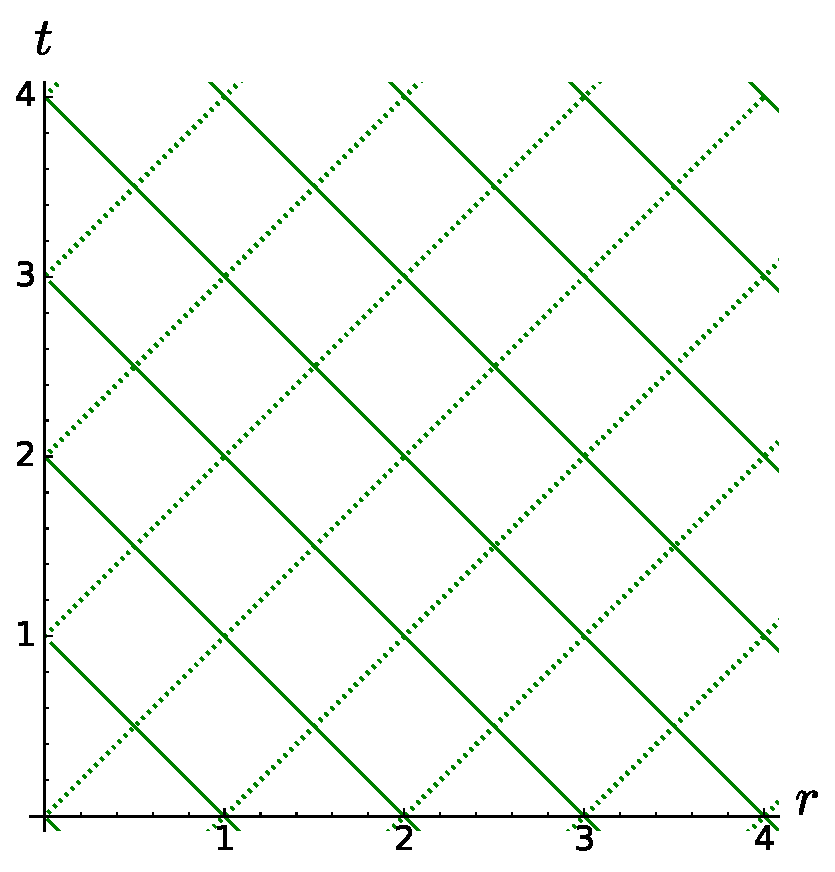
\includegraphics[width=0.5\textwidth]{glo_null_coord.pdf}}
\caption[]{\label{f:glo:null_coord} \footnotesize
Lines of constant null coordinates $u$ (dashed) and $v$
(solid) in terms of the coordinates $(t,r)$.}
\end{figure}


Let us introduce the null coordinate system $(u,v,\th,\ph)$ where $u$ and
$v$ are respectively the retarded\index{retarded!time} and advanced\index{advanced!time}
time defined by (cf. Fig.~\ref{f:glo:null_coord})
\be \label{e:glo:advanced_retarded}
    \left\{ \begin{array}{l}
    u = t - r\\
    v = t + r
    \end{array} \right.
    \iff
    \left\{ \begin{array}{l}
    t = \frac{1}{2} (v+u)\\[1ex]
    r = \frac{1}{2} (v-u) .
    \end{array} \right.
\ee
The metric tensor takes then the shape
\be \label{e:glo:Mink_metric_uv}
    g_{\mu\nu} \D x^\mu \D x^\nu = - \D u \, \D v
        + \frac{1}{4} (v-u)^2 \left(  \D\th^2 + \sin^2\th \, \D\ph^2 \right) .
\ee
The coordinates $(u,v)$ span the half part of $\mathbb{R}^2$ defined by
$u<v$. In order to have coordinates within a finite range, let us consider
their arctangents (cf. Fig.~\ref{f:glo:atan}):
\be \label{e:glo:UV_uv}
    \left\{ \begin{array}{l}
    U = \arctan u \\
    V = \arctan v
    \end{array} \right.
    \iff
   \left\{ \begin{array}{l}
    u = \tan U \\
    v = \tan V .
    \end{array} \right.
\ee
Then the coordinates $(U,V)$ span the half part of $(-\pi/2, \pi/2)\times (-\pi/2, \pi/2)$
defined by $U < V$
(since $\arctan$ is a monotonically increasing function, cf. Fig.~\ref{f:glo:atan}):
\be \label{e:glo:span_UV}
    -\frac{\pi}{2} < U < \frac{\pi}{2}, \quad
    -\frac{\pi}{2} < V < \frac{\pi}{2}, \quad\mbox{and}\quad U < V.
\ee

\begin{figure}
\centerline{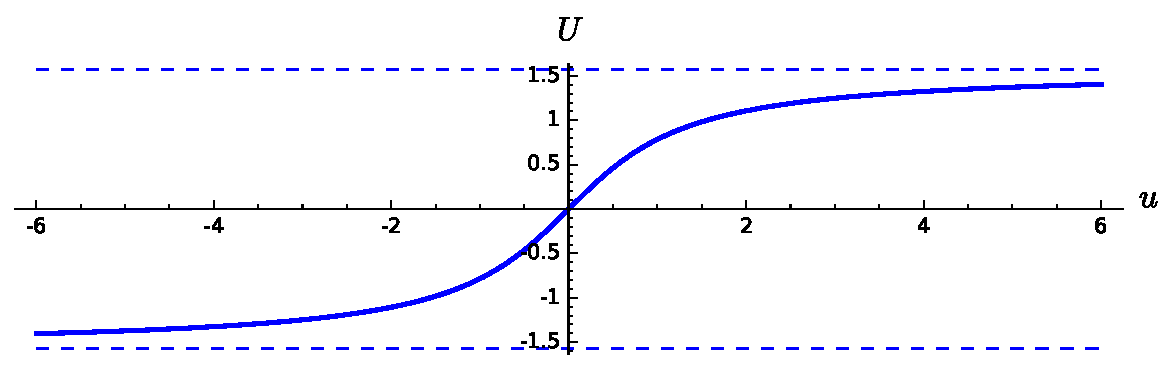
\includegraphics[width=0.8\textwidth]{glo_atan.pdf}}
\caption[]{\label{f:glo:atan} \footnotesize
The arctangent function mapping $\mathbb{R}$ to $(-\pi/2, \pi/2)$.}
\end{figure}

Since
\[
    \D u = \frac{\D U}{\cos^2 U}, \quad \D v = \frac{\D V}{\cos^2 V}
    \quad\mbox{and}\quad
    \tan V - \tan U = \frac{\sin(V-U)}{\cos U \cos V},
\]
the Minkowski metric (\ref{e:glo:Mink_metric_uv})
is expressed in terms of the coordinates $(x^\alpha)=(U,V,\th,\ph)$
as\footnote{See also Sec.~\ref{s:sam:worksheets} for the computation
with SageManifolds.}
\be \label{e:glo:g_UV}
    g_{\mu\nu} \D x^\mu \D x^\nu = \frac{1}{4\cos^2 U \cos^2 V}
    \left[ - 4 \D U \, \D V + \sin^2(V-U) \left(  \D\th^2 + \sin^2\th \, \D\ph^2 \right)
    \right] .
\ee

\begin{remark}
The retarded/advanced times $u$ and $v$ have the dimension of a time, or of a
length in the $c=1$ units that we are using. Therefore, one should introduce
some length scale, $\ell_0$ say, before taking their arctangent and rewrite
(\ref{e:glo:UV_uv}) as
\[
    \left\{ \begin{array}{l}
    U = \arctan (u/\ell_0) \\
    V = \arctan (v/\ell_0)
    \end{array} \right.
    \iff
   \left\{ \begin{array}{l}
    u = \ell_0 \tan U \\
    v = \ell_0 \tan V .
    \end{array} \right.
\]
The coordinates $(U,V)$ are dimensionless and a global factor $\ell_0^2$ should be
introduced in the right-hand side of Eq.~(\ref{e:glo:g_UV}).
However, the length scale $\ell_0$ plays no essential role and, to keep simple notations,
it is omitted in what follows. In other words, we are using units for
which $\ell_0=1$.
\end{remark}

\subsection{Conformal metric}

In the right-hand side of (\ref{e:glo:g_UV}),
the terms in square brackets defines a metric
$\w{\tilde{g}}$ such that
\be \label{e:glo:tilde_g_Omega}
    \encadre{ \w{\tilde{g}} = \Omega^2 \w{g} } ,
\ee
where $\Omega$ is the scalar field $\M \rightarrow \mathbb{R}$ obeying
\begin{subequations}
\begin{align}
    \Omega & =  2 \cos U \cos V \label{e:glo:Omega_UV} \\
           & =  \frac{2}{\sqrt{1+u^2}\sqrt{1+v^2}} \label{e:glo:Omega_uv}\\
           & =  \frac{2}{\sqrt{(t-r)^2+1}\sqrt{(t+r)^2+1}} . \label{e:glo:Omega_tr}
\end{align}
\end{subequations}
We notice on (\ref{e:glo:Omega_uv}) and (\ref{e:glo:Omega_tr}) that the function
$\Omega$ never vanishes on $\M$, so that the bilinear form $\w{\tilde{g}}$ defined by
(\ref{e:glo:tilde_g_Omega}) constitutes a well behaved metric on $\M$.
Moreover, since $\Omega^2 > 0$, $\w{\tilde{g}}$ has the same signature as
$\w{g}$, i.e. $(-,+,+,+)$.
The specific expression of $\w{\tilde{g}}$ is deduced from (\ref{e:glo:g_UV})
and (\ref{e:glo:Omega_UV}):
\be \label{e:glo:tg_UV}
    \tilde{g}_{\mu\nu} \D x^\mu \D x^\nu =  - 4 \D U \, \D V
        + \sin^2(V-U) \left(  \D\th^2 + \sin^2\th \, \D\ph^2 \right) .
\ee

In view of (\ref{e:glo:tilde_g_Omega}), one says that the metric $\w{\tilde{g}}$
is \defin{conformal to}\index{conformal} the metric $\w{g}$, or equivalently,
that the metrics $\w{g}$ and $\w{\tilde{g}}$ are
\defin{conformally related}\index{conformally related metrics},
or that $\w{\tilde{g}}$ arises from $\w{g}$ via a
\defin{conformal transformation}\index{conformal!transformation}.
The scalar field $\Omega$ is called the \defin{conformal factor}\index{conformal!factor}.

A key property of a conformal transformation is to preserve the orthogonality
relations, since (\ref{e:glo:tilde_g_Omega}) clearly
implies, at any point $p\in\M$,
\[
    \forall (\w{u},\w{v})\in T_p\M\times T_p\M,\quad
    \w{\tilde{g}}(\w{u},\w{v}) = 0 \iff \w{g}(\w{u},\w{v}) = 0 .
\]
In particular, null vectors for $\w{\tilde{g}}$ coincide with null vectors for $\w{g}$:
\[
    \forall \wl \in T_p\M,\quad
    \w{\tilde{g}}(\wl,\wl) = 0 \iff \w{g}(\wl,\wl) = 0 .
\]
Consequently the light cones of $(\M,\w{g})$ and $(\M,\w{\tilde{g}})$
are identical.
Moreover, since $\Omega^2>0$, the spacelike and timelike characters of vectors
is preserved as well:
\be
    \begin{array}{ll}
    \forall \w{v} \in T_p\M,\ &
        \w{v} \mbox{\ spacelike for\ } \w{\tilde{g}} \iff \w{v} \mbox{\ spacelike for\ } \w{g} \\
    & \w{v} \mbox{\ timelike for\ } \w{\tilde{g}} \iff \w{v} \mbox{\ timelike for\ } \w{g} .
    \end{array}
\ee
It follows that a curve $\Li$ is timelike (resp. null, spacelike) for $\w{\tilde{g}}$
iff $\Li$ is timelike (resp. null, spacelike) for $\w{g}$. Similarly,
a hypersurface $\Sigma$ is timelike (resp. null, spacelike) for $\w{\tilde{g}}$
iff $\Li$ is timelike (resp. null, spacelike) for $\w{g}$.

What about geodesics? Let us first recall that a null curve is not necessarily
a null geodesic (cf. Remark~\ref{r:def:null_curves} on page~\pageref{r:def:null_curves}),
so that one cannot deduce from the above results that conformal transformations
preserve null geodesics. However, this turns out to be true:
\begin{greybox}
A smooth curve $\Li$ in $\M$ is a null geodesic for $\w{\tilde{g}}$ iff
$\Li$ is a null geodesic for $\w{g}$.
\end{greybox}
To prove it, it suffices to write explicitly the geodesic equation
and to express the Christoffel symbols of $\w{\tilde{g}}$ in terms of those
of $\w{g}$ and the derivatives of $\Omega$ (see e.g. Appendix~D of Wald's
textbook \cite{Wald84} for details).

On the contrary conformal transformations preserve neither the timelike
geodesics nor the spacelike ones.

The coordinates $(U,V)$ are of null type; let us consider instead
the ``time+space'' coordinates $(\tau,\chi)$ defined by\footnote{Notice the
similarity with (\ref{e:glo:advanced_retarded}) up to some $1/2$ factors.}
\be \label{e:glo:tau_chi_U_V}
    \left\{ \begin{array}{l}
    \tau = V + U \\
    \chi = V - U
    \end{array} \right.
    \iff
    \left\{ \begin{array}{l}
    U = \frac{1}{2} (\tau - \chi) \\[1ex]
    V = \frac{1}{2} (\tau + \chi) .
    \end{array} \right.
\ee
Given (\ref{e:glo:span_UV}), the range of these new coordinates is
\be \label{e:glo:range_tau_chi}
    0 < \chi < \pi \quad\mbox{and}\quad
    \chi - \pi < \tau < \pi - \chi .
\ee
In other words, if we draw the Minkowski spacetime in the $(\tau,\chi)$ plane,
it takes the shape of a half-diamond: see Fig.~\ref{f:glo:conf_diag_Mink}.

\begin{figure}
\centerline{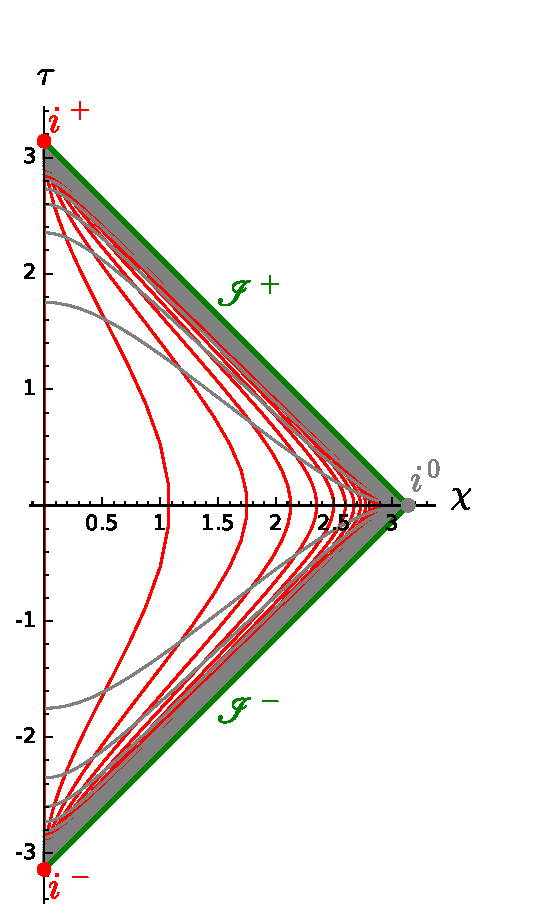
\includegraphics[width=0.5\textwidth]{glo_conf_diag_Mink.pdf}}
\caption[]{\label{f:glo:conf_diag_Mink} \footnotesize
Conformal diagram of Minkowski spacetime. Constant-$r$ curves are drawn in
red, while constant-$t$ ones are drawn in grey.}
\end{figure}

By combining (\ref{e:glo:advanced_retarded}) (\ref{e:glo:UV_uv}) and
(\ref{e:glo:tau_chi_U_V}), we get the link between $(t,r)$ and
$(\tau,\chi)$:
\be \label{e:glo:tau_chi_t_r}
    \left\{ \begin{array}{l}
    \tau = \arctan(t+r) + \arctan(t-r) \\
    \chi = \arctan(t+r) - \arctan(t-r)
    \end{array} \right.
    \iff
    \left\{ \begin{array}{l}
    \displaystyle t = \frac{\sin\tau}{\cos\tau + \cos\chi}\\[2ex]
    \displaystyle r = \frac{\sin\chi}{\cos\tau + \cos\chi} .
    \end{array} \right.
\ee
We may use these relations to draw the lines $t=\mathrm{const}$ and
$r=\mathrm{const}$ in Fig.~\ref{f:glo:conf_diag_Mink}.

The expression of the conformal factor in the
coordinates $(\tau,\chi,\th,\ph)$ is easily deduced from
(\ref{e:glo:Omega_UV}) and
(\ref{e:glo:tau_chi_U_V}):
\be \label{e:glo:Omega_tau_chi}
    \Omega = \cos\tau + \cos\chi .
\ee


\subsection{Conformal completion} \label{s:glo:conf_complet_Mink}

The expression of the conformal metric in terms of the coordinates
$(x^\alpha) = (\tau,\chi,\th,\ph)$ is easily deduced from that in terms of
$(U,V,\th,\ph)$ as given by (\ref{e:glo:tg_UV}):
\be \label{e:glo:tg_Einstein}
    \tilde{g}_{\mu\nu} \D x^\mu \D x^\nu =  - \D\tau^2
        + \D \chi^2
        + \sin^2\chi \left(  \D\th^2 + \sin^2\th \, \D\ph^2 \right) .
\ee
Restricting to a $\tau = \mathrm{const}$ hypersurface, i.e. setting $\D\tau=0$,
we recognize the standard metric of the hypersphere
$\mathbb{S}^3$ in the hyperspherical coordinates $(\chi,\th,\ph)$.
Moreover, we notice that the full metric (\ref{e:glo:tg_Einstein})
is perfectly regular even if we relax
the condition on $\tau$ in (\ref{e:glo:range_tau_chi}), i.e. if we
let $\tau$ span the
entire $\mathbb{R}$. We may then consider the manifold
\be
    \mathscr{E} = \mathbb{R}\times \mathbb{S}^3
\ee
and $\w{\tilde{g}}$ as a Lorentzian metric on $\mathscr{E}$ given by
(\ref{e:glo:tg_Einstein}).
The Lorentzian manifold
$(\mathscr{E},\w{\tilde{g}})$ is nothing but the
\defin{Einstein static universe}\index{Einstein!static universe}\index{static!universe (Einstein)}, also called the \defin{Einstein cylinder}\index{Einstein!cylinder}\index{cylinder!Einstein --},
a static solution of the Einstein equation (\ref{e:bas:Einstein_eq})
with $\Lambda > 0$ and some pressureless matter of uniform density
$\rho = \Lambda/(4\pi)$.
We have thus an embedding\footnote{Cf. Sec.~\ref{s:bas:embed} of Appendix~A} of Minkowski spacetime into the Einstein cylinder:
\be \label{e:glo:embed_Mink_Einst}
     \Phi:\ \M \longrightarrow \mathscr{E}
\ee
and this embedding is a conformal isometry from
$(\M,\w{g})\rightarrow (\Phi(\M),\w{\tilde{g}})$.
In the following, we shall identify $\Phi(\M)$ and $\M$, i.e. use the same
symbol $\M$ to denote the subset of $\mathscr{E}$ that is the image of $\M$ via the
embedding (\ref{e:glo:embed_Mink_Einst}).

\begin{figure}
\centerline{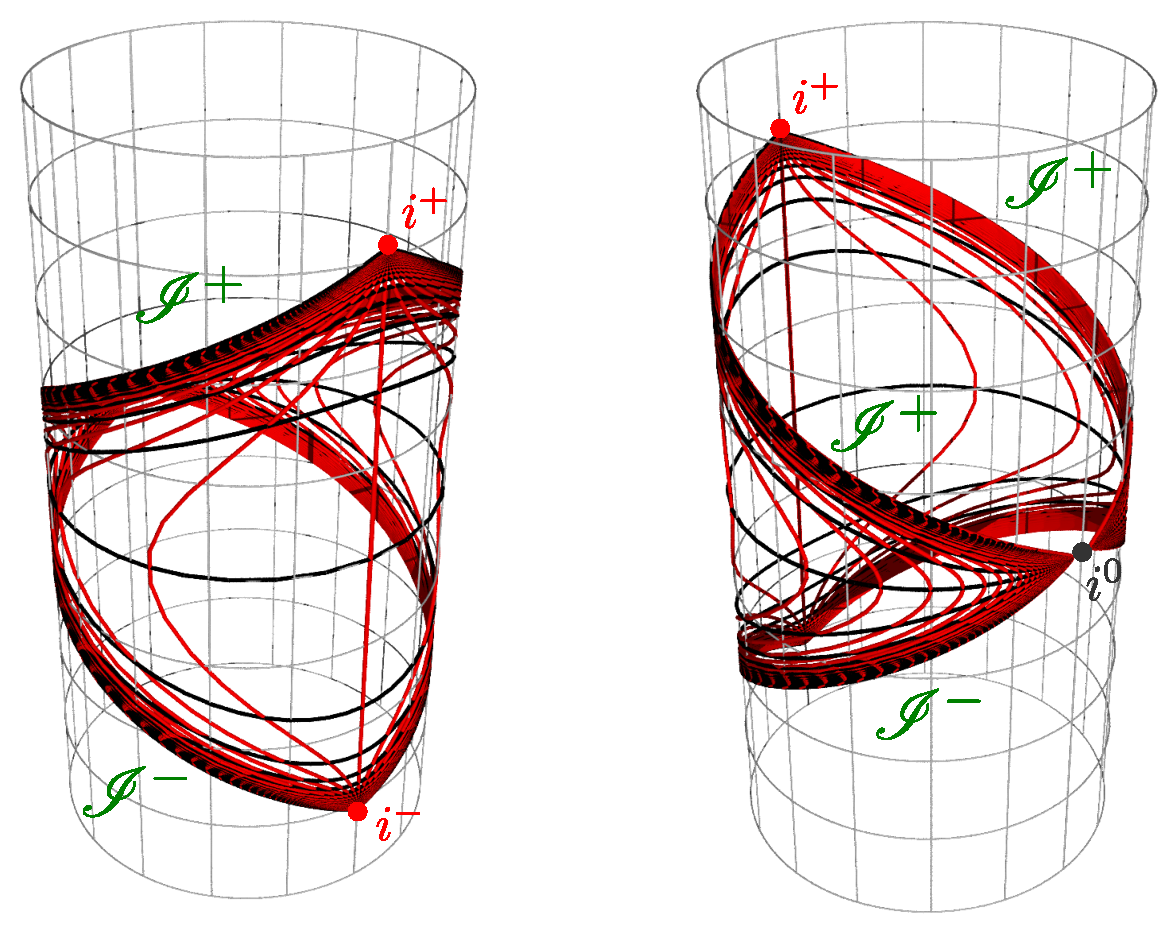
\includegraphics[width=0.6\textwidth]{glo_Einstcyl_Mink.pdf}}
\caption[]{\label{f:glo:Einstcyl_Mink}\footnotesize
Two views of the Einstein cylinder $\mathscr{E}$, with the conformal embedding of
Minkowski spacetime in it.
The red curves are the same constant-$r$ curves
as in Fig.~\ref{f:glo:conf_diag_Mink}, while the black curves are
the same constant-$t$ curves as those drawn in grey in Fig.~\ref{f:glo:conf_diag_Mink}.}
\end{figure}

Since $\mathscr{E}$ and $\M$ have the same dimension, $\M$ is an open subset of $\mathscr{E}$.
Its closure $\overline{\M}$ in $\mathscr{E}$ is (cf.
Figs.~\ref{f:glo:conf_diag_Mink} and \ref{f:glo:Einstcyl_Mink})
\be
    \overline{\M} = \M \cup \scri^+ \cup \scri^- \cup \left\{ i^0 \right\} \cup
            \left\{ i^+ \right\} \cup \left\{ i^- \right\} ,
\ee
where
\begin{itemize}
\item $\scri^+$ is the hypersurface of $\mathscr{E}$ defined by
$\tau = \pi - \chi$ and $0 < \tau < \pi$;
\item $\scri^-$ is the hypersurface of $\mathscr{E}$ defined by
$\tau = \chi - \pi $ and $-\pi  < \tau < 0$;
\item $i^0$ is the point of $\mathscr{E}$ defined by $\tau=0$ and $\chi=\pi$;
\item $i^+$ is the point of $\mathscr{E}$ defined by $\tau=\pi$ and $\chi=0$;
\item $i^-$ is the point of $\mathscr{E}$ defined by $\tau=-\pi$ and $\chi=0$.
\end{itemize}
It is customary to pronounce $\scri$ as ``scri'', for \emph{script i}.

\begin{remark}
On $\mathbb{S}^3$, the hyperspherical coordinates $(\chi,\th,\ph)$
are singular at $\chi=0$ and $\chi=\pi$, so that setting $\chi=0$ (or $\chi=\pi$)
defines a unique point of $\mathbb{S}^3$, whatever the value of $(\th,\ph)$.
Note also that the vertical left boundary of the diamond drawn in
Fig.~\ref{f:glo:conf_diag_Mink}, i.e. the segment defined by
$\tau\in(-\pi,\pi)$ and $\chi=0$, is \emph{not} a part of the boundary
of $\M$ but merely reflect the coordinate singularity at $\chi=0$, in the same
way that the left vertical boundary of Fig.~\ref{f:glo:null_coord}
is not a boundary of Minkowski spacetime but is
due to the coordinate singularity at $r=0$. Note by the way that
$\chi=0$ implies $r=0$ via (\ref{e:glo:tau_chi_t_r}).
\end{remark}

Let
\be
    \scri := \scri^+ \cup \scri^-
\ee
and
\be
    \tilde{\M} := \M \cup \scri .
\ee
$\tilde{\M}$ is naturally a smooth manifold with
boundary\footnote{Cf. Sec.~\ref{s:bas:manif_boundary} for the precise definition.}\index{manifold!with boundary}
and its boundary is $\scri$:
\be
    \partial \tilde{\M} = \scri.
\ee
\begin{remark}
Because closure $\overline{\M}$ is self-intersecting at the point $i^0$
(cf. Fig.~\ref{f:glo:Einstcyl_Mink}), it is not a manifold with boundary: no open neighbourhood of
$i^0$ is homeomorphic to a neighbourhood of $[0,+\infty)\times \mathbb{R}^2$.
At the points $i^+$ and $i^-$, $\overline{\M}$ can be considered as a
topological manifold with boundary, but not as a \emph{smooth} manifold with boundary.
Hence the three points $i^0$, $i^+$ and $i^-$ are excluded from the definition
of the manifold with boundary $\tilde{\M}$.
\end{remark}

\begin{figure}
\centerline{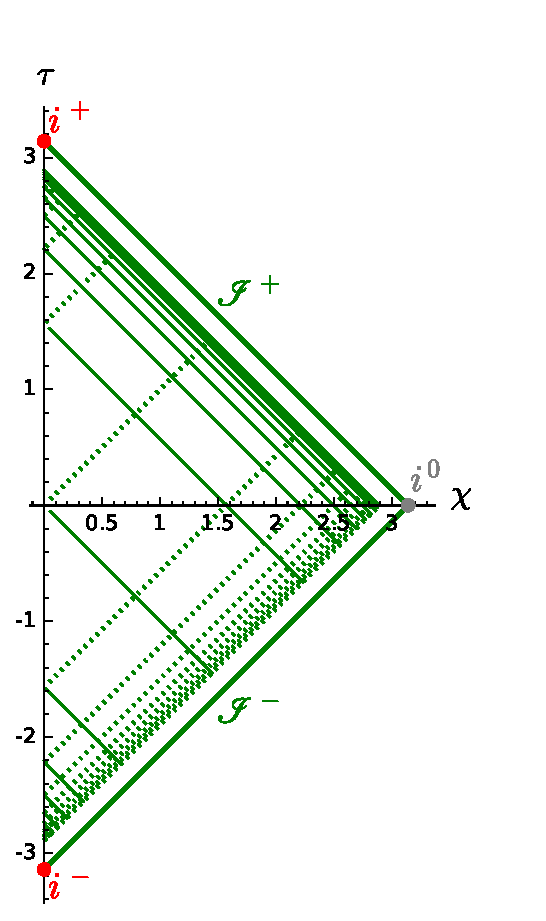
\includegraphics[width=0.45\textwidth]{glo_conf_Mink_null.pdf}}
\caption[]{\label{f:glo:conf_Mink_null}\footnotesize
Null radial geodesics in the conformal diagram of Minkowski spacetime.
The dashed green lines are null geodesics $u=\mathrm{const}$ for
17 values of $u$ uniformly spanning $[-8,8]$, while the solid green lines are
null geodesics $v=\mathrm{const}$ for 17 values of $v$ uniformly spanning $[-8,8]$.}
\end{figure}

The hypersurface $\scri^+$ is the location of $\tilde{\M}$ where all radial null geodesics
terminate, while $\scri^-$ is the location of $\tilde{\M}$ where all these geodesics originate (cf. Fig.~\ref{f:glo:conf_Mink_null}). For this
reason $\scri^+$ is called the
\defin{future null infinity}\index{future!null infinity}\index{null!infinity}
of $(\M,\w{g})$
and $\scri^-$ the \defin{past null infinity}\index{past!null infinity}
of $(\M,\w{g})$.
On the other side, any timelike geodesic of $(\M,\w{g})$ originates at $i\-$ and ends at
$i^+$ (cf. Fig.~\ref{f:glo:conf_diag_Mink}), while any spacelike geodesic
of $(\M,\w{g})$ originates at $i^0$ and terminates there
(after having completed a closed path on $\mathbb{S}^3$ (cf. Fig.~\ref{f:glo:Einstcyl_Mink}).
The point $i^+$ is then called the
\defin{future timelike infinity}\index{future!timelike infinity}\index{timelike!infinity}
of $(\M,\w{g})$,
$i\-$ the \defin{past timelike infinity}\index{past!timelike infinity}
of $(\M,\w{g})$
and $i^0$ the \defin{spacelike infinity}\index{spacelike!infinity} of $(\M,\w{g})$.

As it is clear on the conformal diagram of Fig.~\ref{f:glo:conf_diag_Mink},
both $\scri^+$ and $\scri^-$ are null hypersurfaces of $(\tilde{\M},\w{\tilde{g}})$.

\begin{figure}
\centerline{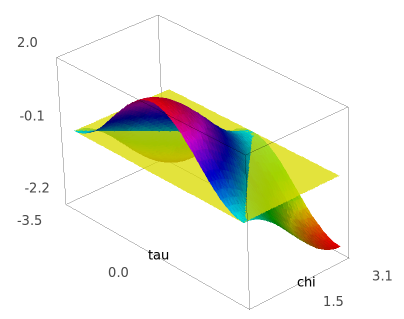
\includegraphics[width=0.45\textwidth]{glo_Omega_Mink.png}}
\caption[]{\label{f:glo:Omega_Mink}\footnotesize
Conformal factor $\Omega$ as a function of $(\tau,\chi)$ [cf. Eq.~(\ref{e:glo:Omega_tau_chi})].}
\end{figure}


It is precisely because $\Omega$ vanishes (cf. Fig.~\ref{f:glo:Omega_Mink}) at the boundary
\be
    \overline{\M} \setminus \M = \scri^+ \cup \scri^- \cup \left\{ i^0 \right\} \cup
            \left\{ i^+ \right\} \cup \left\{ i^- \right\}
\ee
that the conformal transformation (\ref{e:glo:tilde_g_Omega}) brings infinity
of Minkowski space to a finite distance.


%%%%%%%%%%%%%%%%%%%%%%%%%%%%%%%%%%%%%%%%%%%%%%%%%%%%%%%%%%%%%%%%%%%%%%%%%%%%%%%%%%%%%%%%

\section{Conformal completions and asymptotic flatness} \label{s:glo:conf_compl}

Having investigated the asymptotic structure of Minkowski spacetime
via a conformal completion, let us use the latter to define spacetimes
that ``look like'' Minkowski spacetime asymptotically: we
shall say that a spacetime $(\M,\w{g})$ admits a
\defin{conformal completion}\index{conformal!completion}
iff there exists a Lorentzian manifold with boundary
$(\tilde{\M},\w{\tilde{g}})$ equipped with a smooth non-negative scalar field
$\Omega: \tilde{\M} \rightarrow \mathbb{R}^+$
such that
\begin{enumerate}
\item $\tilde{\M} = \M \cup \scri$, with $\scri := \partial \tilde{\M}$
(the boundary of $\tilde{\M})$;
\item on $\M$, $\w{\tilde{g}} = \Omega^2 \w{g}$;
\item on $\scri$, $\Omega=0$;
\item on $\scri$, $\dd \Omega \not= 0$.
\end{enumerate}
Condition~1 expresses that $\M$ has been endowed with some boundary.
A rigorous formulation of it would be via an embedding $\Phi:\M \rightarrow \tilde{\M}$,
as in Eq.~(\ref{e:glo:embed_Mink_Einst}), so that
$\tilde{\M} = \Phi(\M) \cup \scri$. However, as above, we identify $\Phi(\M)$
with $\M$ and therefore simply write $\tilde{\M} = \M \cup \scri$.
Conditions~2 and 3 express that the boundary of $\M$, which ``lies at an infinite
distance'' with respect to $\w{g}$, has been brought to a
finite distance with respect to $\w{\tilde{g}}$. Indeed, in terms of
length elements, condition~2
implies
\[
    \D s^2 = \frac{1}{\Omega^2} \, \D {\tilde s}^2
\]
with $1/\Omega^2 \rightarrow +\infty$ as one approaches $\scri$
(condition~3).
 Finally, condition~4 ensures
that $\scri$ is a regular hypersurface of $\tilde{\M}$.
It is of course fulfilled by Minkowski spacetime, as we can check graphically
on Fig.~\ref{f:glo:Omega_Mink}: the graph of $\Omega$ has no horizontal slope
at $\scri$.

\begin{remark}
When we say that $(\tilde{\M},\w{\tilde{g}})$ is a Lorentzian manifold with
boundary, this implies that $\w{\tilde{g}}$ is smooth everywhere on $\tilde{\M}$,
including at the boundary $\scri$.
\end{remark}

\begin{example}[conformal completion of AdS$_{n}$ spacetime]
... to be completed ... \\
$\scri$ is timelike
\end{example}

More generally, if $\w{g}$ is a solution of Einstein vacuum equation with
a cosmological constant $\Lambda$ [Eq.~(\ref{e:bas:Einstein_eq})], then
\begin{itemize}
\item $\scri$ is a null hypersurface if $\Lambda=0$;
\item $\scri$ is a spacelike hypersurface if $\Lambda>0$;
\item $\scri$ is a timelike hypersurface if $\Lambda<0$.
\end{itemize}
\begin{proof}
... to be completed ...
\end{proof}



Furthermore, one says that $(\tilde{\M},\w{\tilde{g}})$ is a
\defin{conformal completion at null infinity}\index{conformal!completion!at null infinity}
of $(\M,\w{g})$
iff $(\tilde{\M},\w{\tilde{g}})$  is a conformal completion such that
\be
    \scri = \scri^+ \cup \scri^-,
\ee
with $\scri^+$ (resp. $\scri^-$) being never intersected by any past-directed
(resp. future-directed) causal
curve originating in $\M$. Let us recall that a
\defin{causal curve}\index{causal!curve} is
curve whose tangent vectors are nowhere spacelike.
As for Minkowksi spacetime, we shall call $\scri^+$ the
\defin{future null infinity}\index{future!null infinity}\index{null!infinity}
and $\scri^-$ the \defin{past null infinity}\index{past!null infinity}
of $(\M,\w{g})$.

\begin{remark}
One often speaks about \emph{conformal compactification}\index{conformal!compactification}
instead of \emph{conformal completion}, but in general $\tilde{\M}$ is not a
compact manifold. For instance, because we omitted the points $i^+$, $i^-$ and $i^0$,
$\tilde{\M}$ is not compact even for Minkowski spacetime.
\end{remark}

\begin{remark}
Note that the above definition of $\scri^+$ and $\scri^-$ does not impose
that these two objects are null hypersurfaces of $(\tilde{\M},\w{\tilde{g}})$.
This is true for Minkowski spacetime, but not necessarily for other spacetimes,
as the following example shows.
\end{remark}

\begin{example}[Conformal completion of dS$_{n}$ spacetime]
... to be completed ... \\
$\scri^+$ and $\scri^-$ are spacelike
\end{example}


Penrose \cite{Penro64,Penro68} has defined
a spacetime $(\M,\w{g})$ to be \defin{asymptotically simple}\index{asymptotically!simple} iff there exists
a conformal completion $(\tilde{\M},\w{\tilde{g}})$
of $(\M,\w{g})$
such that every null geodesic in $\M$ has two endpoints in $\scri$.

The last condition, which is verified by Minkowski spacetime (cf. Fig.~\ref{f:glo:conf_Mink_null}), is rather restrictive. In particular, it excludes
black hole spacetimes, since, almost by definition, the latter contain null
geodesics that have no endpoint on $\scri^+$, having only a past endpoint
on $\scri^-$, as far as $\scri$ is concerned. To cope with these spacetimes,
Penrose \cite{Penro68} has introduced the following definition:
a spacetime $(\M,\w{g})$ is
\defin{weakly asymptotically simple}\index{weakly!asymptotically simple} iff
there exists an open subset $\mathscr{U}$ of $\M$ and
an asymptotically simple spacetime $(\M_0, \w{g}_0)$
with an open neighbourhood $\mathscr{U}_0$ of $\scri_0 = \partial \tilde{\M}_0$
in $\tilde{\M}_0$ such that $(\mathscr{U}_0\cap \M_0,\w{g}_0)$ is
isometric to $(\mathscr{U},\w{g})$.

\begin{remark}
For a given weakly asymptotically simple spacetime, there may be different
(non overlapping) regions $\mathscr{U}$ satisfying the above property.
For instance we shall see in Chap.~\ref{s:ker}
that there are an infinite series of them in the Kerr spacetime.
\end{remark}

Finally one says that a spacetime $(\M,\w{g})$ is
\defin{asymptotically flat}\index{asymptotically!flat}\index{flat!asymptotically --}
(or more precisely \defin{weakly asymptotically simple and empty}\index{weakly!asymptotically simple and empty} \cite{HawkiE73})
iff $(\M,\w{g})$ is weakly asymptotically simple and the Ricci tensor of
$\w{g}$ vanishes in an open neighbourhood of $\scri$: $\w{R} = 0$.

\begin{example}
The de Sitter and anti-de Sitter spacetimes are asympotically simple but
are not asymptotically flat.
\end{example}

Penrose \cite{Penro65b} (see also \cite{Fraue04}) has shown that if $(\M,\w{g})$
is asymptotically simple and empty, that the Weyl tensor of $\w{g}$ (cf. Sec.~\ref{s:bas:Weyl})
vanishes at $\scri$. Since the
Ricci tensor is zero, this implies that the full Riemann curvature tensor vanishes
at $\scri$ [cf. Eq.~(\ref{e:bas:Weyl})], hence the qualifier \emph{asymptotically flat}.

%%%%%%%%%%%%%%%%%%%%%%%%%%%%%%%%%%%%%%%%%%%%%%%%%%%%%%%%%%%%%%%%%%%%%%%%%%%%%%%%%%%%%%%%

\section{Black holes} \label{s:glo:BH}

\subsection{Preliminaries regarding causal structure}

Before we proceed to the precise definition of a black hole, let us introduce
some concepts regarding the causal structure of a given spacetime $(\M,\w{g})$.
For any subset $S$ of $\M$, one defines
\begin{itemize}
\item the \defin{chronological future of $S$}\index{chronological!future} as the set $I^+(S)$ of all
points of $\M$ that can be reached from a point of $S$ by a future-directed
timelike curve of nonzero extent;
\item the \defin{causal future of $S$}\index{causal!future} as the set $J^+(S)$ of
all points that either are in $S$ or can be reached from a point of $S$ by a future-directed
causal curve;
\item the \defin{chronological past of $S$}\index{chronological!past} as the set $I^-(S)$ of all
points of $\M$ that can be reached from a point of $S$ by a past-directed
timelike curve of nonzero extent;
\item the \defin{causal past of $S$}\index{causal!past} as the set $J^-(S)$ of
all points that either are in $S$ or can be reached from a point of $S$ by a past-directed
causal curve.
\end{itemize}
From the above definitions, one has always $S \subset J^\pm(S)$ and
$I^\pm(S) \subset J^\pm(S)$.

\begin{remark}
One has not necessarily $S \subset I^\pm(S)$. For instance,
if the spacetime does not contain
any closed timelike curve, one has  $S \cap I^\pm(S) = \varnothing$ for
$S = \{p\}$ with $p$ any point of $\M$.
\end{remark}

Here are some basic topological properties of the future and past sets
defined above (see e.g. \S~6.2 of \cite{HawkiE73} or Chap.~14 of
\cite{ONeil83} for proofs):
\begin{itemize}
\item
$I^\pm(S)$ is always an open subset\footnote{This property is a direct
consequence of Lemma~1 in Sec.~\ref{s:glo:properties_H} below.} of $\M$, while
$J^\pm(S)$ is not necessarily a closed subset.
\item The interior of $J^\pm(S)$ is $I^\pm(S)$:
\be \label{e:glo:int_JS_IS}
    \mathrm{int}\, J^\pm(S) = I^\pm(S).
\ee
\item Both sets have the same closure:
\be \label{e:glo:clos_JS_IS}
    \overline{J^\pm(S)} = \overline{I^\pm(S)} .
\ee
\item
It follows from (\ref{e:glo:int_JS_IS}) and (\ref{e:glo:clos_JS_IS})
that both sets share the same boundary:
\be \label{e:glo:boundary_JS_IS}
    \partial J^\pm(S) = \partial I^\pm(S).
\ee
\end{itemize}

\subsection{General definition of a black hole} \label{s:glo:def_BH}

We are now in position to give the general definition of a black hole.
We shall do it for a spacetime $(\M,\w{g})$ that admits a conformal completion
at null infinity as defined in Sec.~\ref{s:glo:conf_compl} and thus
possesses a future null infinity $\scri^+$.
Moreover, we shall assume that $\scri^+$ is \defin{complete}\index{complete!future null infinity}: if $\scri^+$
is a null hypersurface, which occurs if $(\M,\w{g})$ is asymptotically flat,
this means that $\scri^+$ is generated by complete null geodesics.
The completeness condition is imposed to avoid ``spurious'' black holes,
such as black holes in Minkowski space (cf. Remark~\ref{s:glo:spurious_bh} below).
The neighbourhood of $\scri^+$
in $\tilde{\M}$ can then be considered as the infinitely far region
reached by outgoing null geodesics. If a null geodesic does not reach this
region, it can be considered as being trapped somewhere else in spacetime: this
``somewhere else'' constitutes the black hole region.

\begin{greybox}
Let $(\M,\w{g})$ be a spacetime with a conformal completion at null infinity
such that $\scri^+$ is complete;
the \defin{black hole region}\index{black!hole}, or simply \defin{black hole},
is the set of points of $\M$ that are not in the causal past of the future null infinity:
\be \label{e:glo:def_BH}
    \encadre{\mathscr{B} := \M \setminus (J^-(\scri^+)\cap\M) } .
\ee
(cf. Fig.~\ref{f:glo:def_bh}).
\end{greybox}
The black hole region is thus the set of points of $\M$
from which no future-directed causal curve in $\tilde{\M}$ reaches $\scri^+$.
Of course, it may be that $\mathscr{B} = \varnothing$, in which case one
says that the spacetime $(\M,\w{g})$ contains no black hole.


\begin{figure}
\centerline{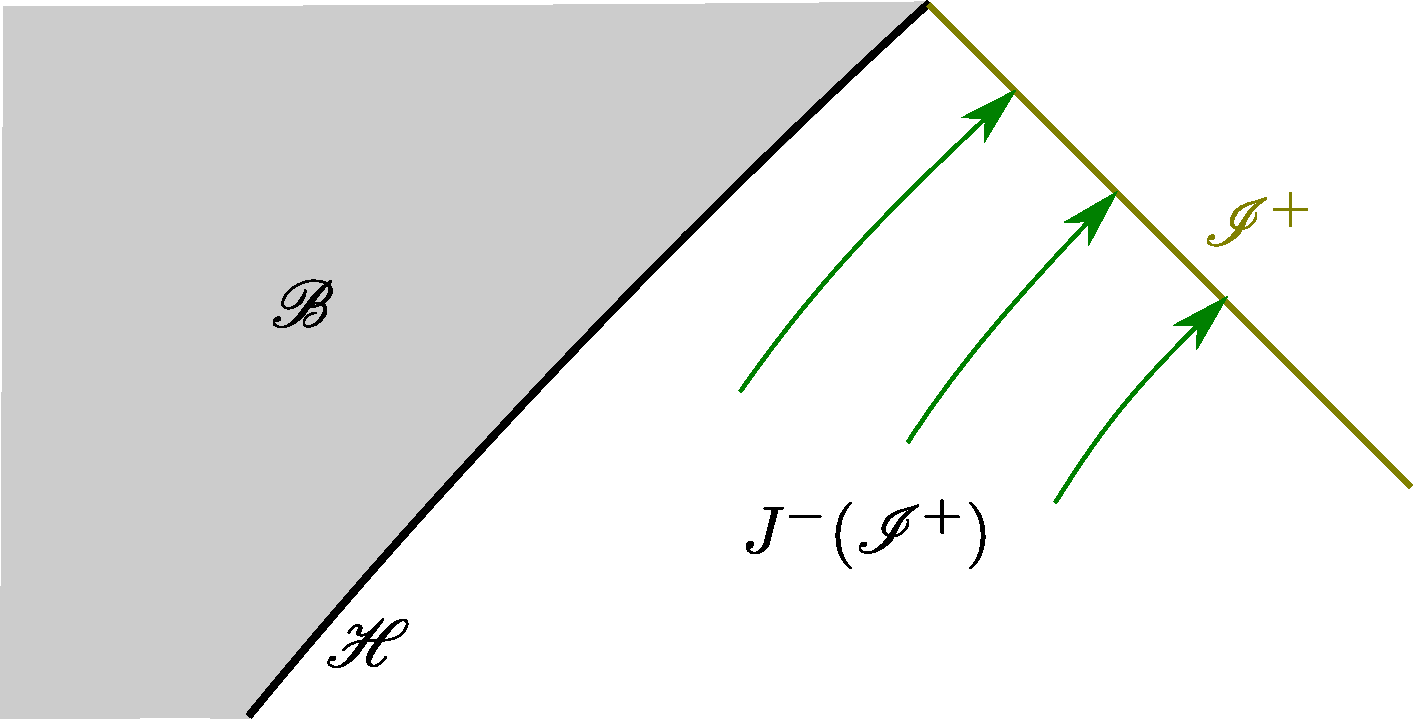
\includegraphics[width=0.6\textwidth]{glo_def_bh.pdf}}
\caption[]{\label{f:glo:def_bh} \footnotesize
The black hole region $\mathscr{B}$ defined as the complement of
the causal past of the future null infinity, $J^-(\scri^+)$.}
\end{figure}


\begin{example}
The Minkowski spacetime contains no black hole, for all future-directed null geodesics
terminate at $\scri^+$ (cf. Fig.~\ref{f:glo:conf_Mink_null}).
More generally, any asymptotically simple spacetime contains no black hole.
\end{example}

\begin{remark} \label{s:glo:spurious_bh}
If we release the assumption of $\scri^+$-completeness in the above definition,
we may end up with unphysical or ``spurious'' black holes.
For instance, let us consider the conformal completion of Minkowski spacetime
$(\M,\w{g})$ resulting from its embedding in the Einstein cylinder
$(\E,\w{\tilde{g}})$, as in
Sec.~\ref{s:glo:conf_complet_Mink},
keeping the same $\scri^-$ but
defining $\scri^+$ as the
hypersurface of $\E$ given by $\tau = \pi - \chi$
and $0<\tau<\pi/2$, instead of  $0<\tau<\pi$ in Sec.~\ref{s:glo:conf_complet_Mink}.
The manifold with boundary $\tilde{\M} := \M \cup \scri^+ \cup \scri^-$,
equipped with the Einstein cylinder metric $\w{\tilde g}$, is then a conformal completion
of $(\M,\w{g})$ at null infinity. With such a $\scri^+$, the black hole region
defined by (\ref{e:glo:def_BH}) is non-empty, as shown in Fig.~\ref{f:glo:spurious_bh}.
\end{remark}

\begin{figure}
\centerline{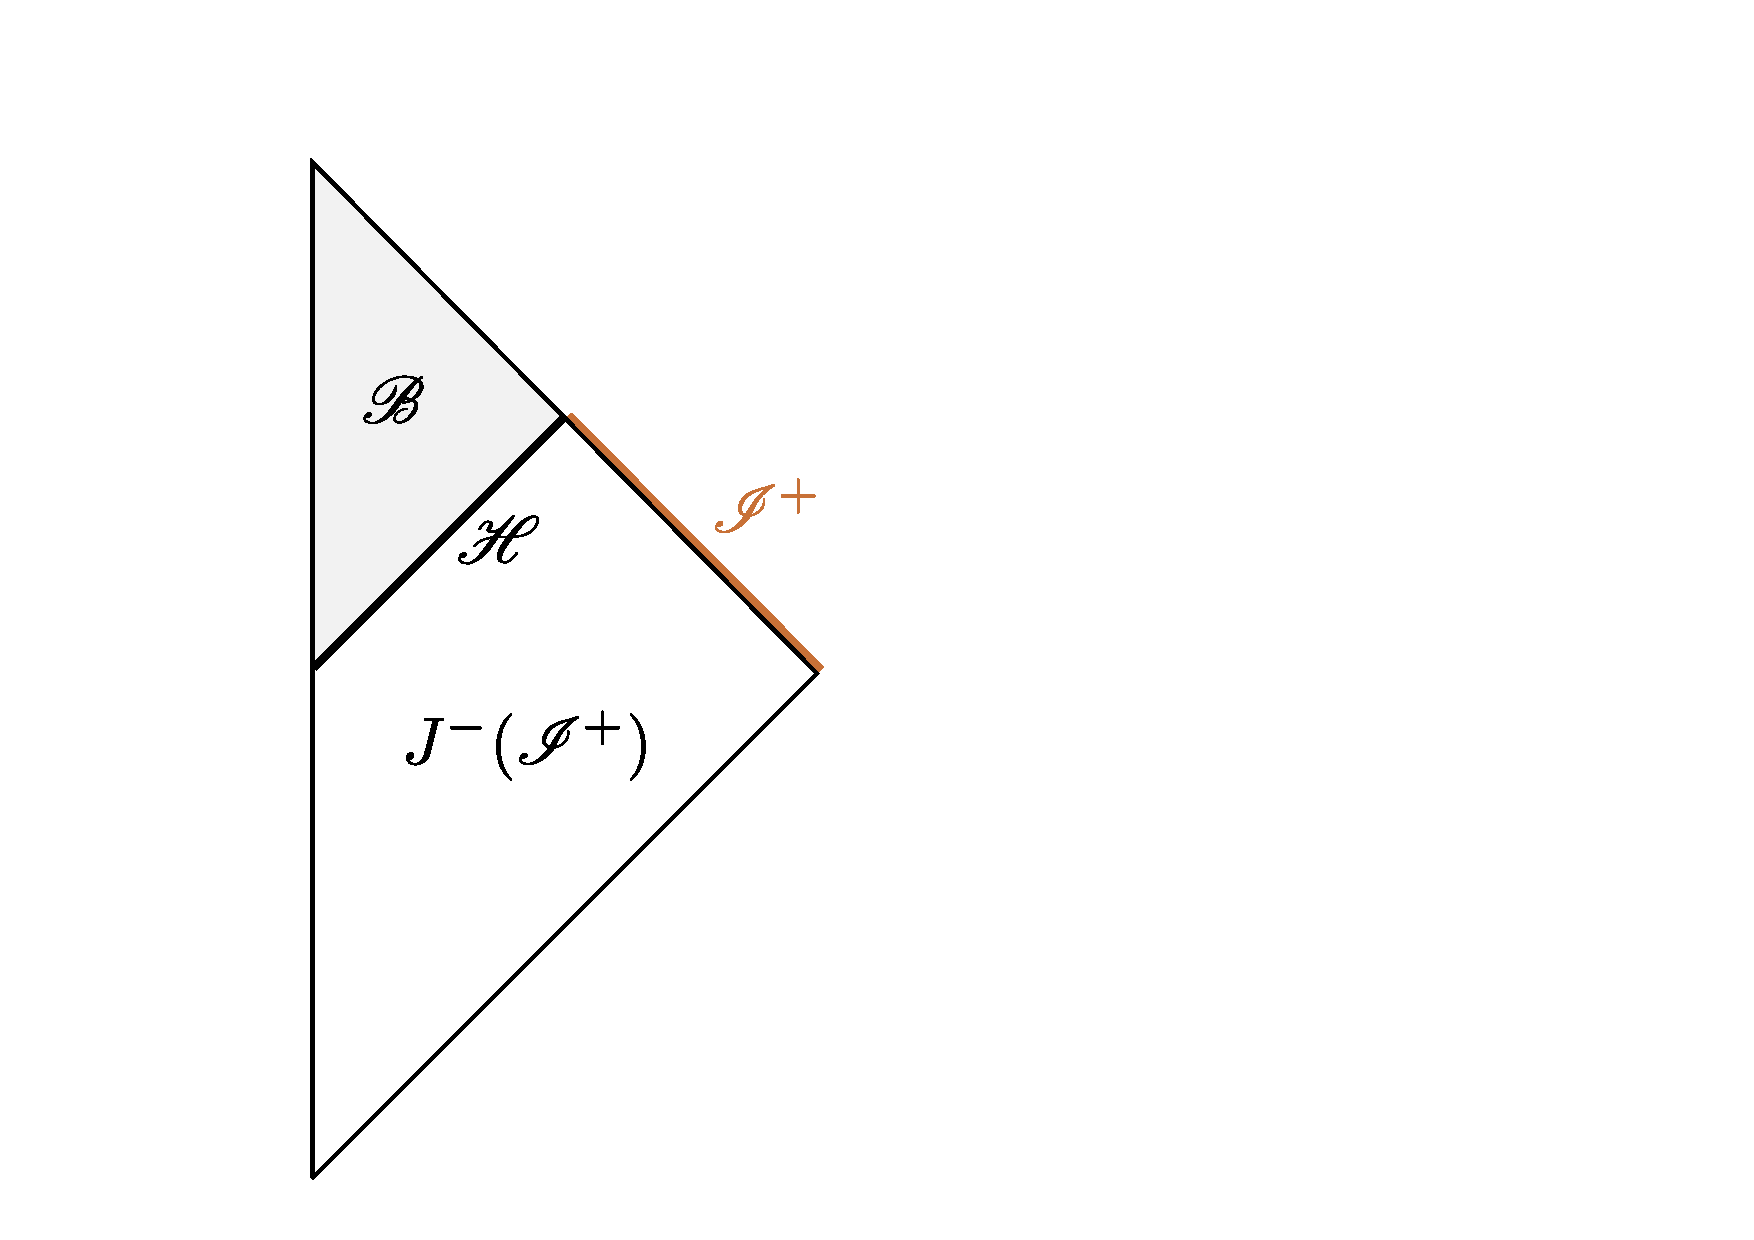
\includegraphics[height=0.3\textheight]{glo_spurious_bh.pdf}}
\caption[]{\label{f:glo:spurious_bh} \footnotesize
Spurious black hole region $\mathscr{B}$ in Minkowski spacetime resulting
from a conformal completion with a non-complete $\scri^+$.
Compare with Fig.~\ref{f:glo:conf_Mink_null}.}
\end{figure}



\begin{remark}
Some authors (in particular Hawking and Ellis \cite{HawkiE73}) define a
\emph{black hole} as a connected component of
$S(\tau) \cap \mathscr{B}$, where $S(\tau)$ is a spacelike
hypersurface that is a slice of the future development of a partial
Cauchy hypersurface $S(0)$ such that the
closure in $\tilde{\M}$ of the domain of dependence of $S(0)$ contains $\scri^+$.
According to such a definition, a black hole is a $(n-1)$-dimensional object,
while the black hole $\mathscr{B}$ defined above is a $n$-dimensional object.
\end{remark}

If $\mathscr{B}\not=\varnothing$, the boundary $\Hor$ of the black hole region
is called the \defin{future event horizon}\index{future!event horizon}
(or simply the \defin{event horizon}\index{event!horizon}
when no ambiguity may arise):
\be
    \encadre{\Hor := \partial \mathscr{B}}.
\ee
By pluging expression (\ref{e:glo:def_BH}) for $\mathscr{B}$ in the standard
identity $\partial \mathscr{B} =
\overline{\mathscr{B}} \cap \overline{\M\setminus \mathscr{B}}$, we get
an equivalent expression for $\Hor$:
\[
    \Hor = \overline{\M \setminus (J^-(\scri^+)\cap\M)} \cap
        \overline{(J^-(\scri^+)\cap\M)}
        = \partial(J^-(\scri^+)\cap\M) .
\]
Now, the boundary of $J^-(\scri^+)$ in $\tilde{\M}$ is
$\partial J^-(\scri^+) = \partial (J^-(\scri^+)\cap\M) \cup \scri^+$, so that
$\partial J^-(\scri^+) \cap \M =  \partial(J^-(\scri^+)\cap\M)$; hence
\be
    \encadre{\Hor = \partial J^-(\scri^+) \cap \M }.
\ee
In words: the future event horizon $\Hor$ is the part of the boundary of the causal past
of the future null infinity $\scri^+$ that lies in $\M$ (cf. Fig.~\ref{f:glo:def_bh}).
Note that thanks to identity (\ref{e:glo:boundary_JS_IS}), we can write as
well
\be
    \Hor = \partial I^-(\scri^+) \cap \M .
\ee

In a way symmetric to the black hole one, one defines
the \defin{white hole region}\index{white!hole} of a
spacetime $(\M,\w{g})$ with a conformal completion at null infinity as the
complement within $\M$ of the causal future of the past null infinity.
\be
    \encadre{\mathscr{W} := \M \setminus (J^+(\scri^-)\cap \M) } .
\ee
The white hole region is thus the set of points of $\M$
from which no past-directed causal curve in $\tilde{\M}$ reaches $\scri^-$.
The boundary of white hole region is called the
\defin{past event horizon}\index{past!event horizon}:
\be
    \encadre{\Hor^- := \partial \mathscr{W} = \partial J^+(\scri^-) \cap \M } .
\ee

The \defin{domain of outer communications}\index{domain!of outer communications}
is the part $\langle\langle \M\rangle\rangle$ of $\M$ that lies neither
in the black hole region nor in the white hole one:
\be
    \langle\langle \M\rangle\rangle := \M\setminus (\mathscr{B}\cup \mathscr{W} )
            = \left( J^-(\scri^+) \cap J^+(\scri^-) \right) \cap \M .
\ee
The last equality, which is a direct consequence of the definitions of
$\mathscr{B}$ and $\mathscr{W}$, shows that the domain of outer communications
is the set of points from which it is possible to send a signal to and to
receive a signal from arbitrary far regions.
It also follows immediately from the definitions of the two event horizons
that the boundary of the domain of outer communications is their union:
\be
    \partial \langle\langle \M\rangle\rangle  = \Hor \cup \Hor^- .
\ee

\begin{hist}
The term \emph{event horizon} has been introduced by W.~Rindler in 1956 \cite{Rindl56}
in the context of a single observer moving in some cosmological spacetime.
The word \emph{black hole} has been coined by J.A.~Wheeler in the end of 1967,
from a suggestion shouted from the audience during one of his conference.
It superseded the previous names
\emph{frozen star}, \emph{collapsed star}, or \emph{astre occlus}
(the latter appearing along \emph{black holes} in the title of
the proceedings of the famous Les Houches summer school of 1972 \cite{DeWit73}).
The expression \emph{domain of outer communications} is due to B.~Carter
(1971) \cite{Carte71}.
\end{hist}


\subsection{Properties of the future event horizon} \label{s:glo:properties_H}

Having defined a black hole in full generality, let us derive the
main properties of the black hole boundary: the event horizon $\Hor$.

\subsubsection{Property 1:}
\begin{greybox}
$\Hor$ is an \defin{achronal set}\index{achronal set}, i.e. no pair of points of $\Hor$ can be connected
by a timelike curve of $\M$.
\end{greybox}

Note that in the definition of an achronal set, it is not demanded that the timelike
curve lies entirely in the set (for instance, the set can be discrete, so that no curve
whatsoever lies in it). Accordingly,
an equivalent statement of Property~1 is: no timelike curve of $\M$
encounters $\Hor$ at more than one point.

\begin{figure}
\centerline{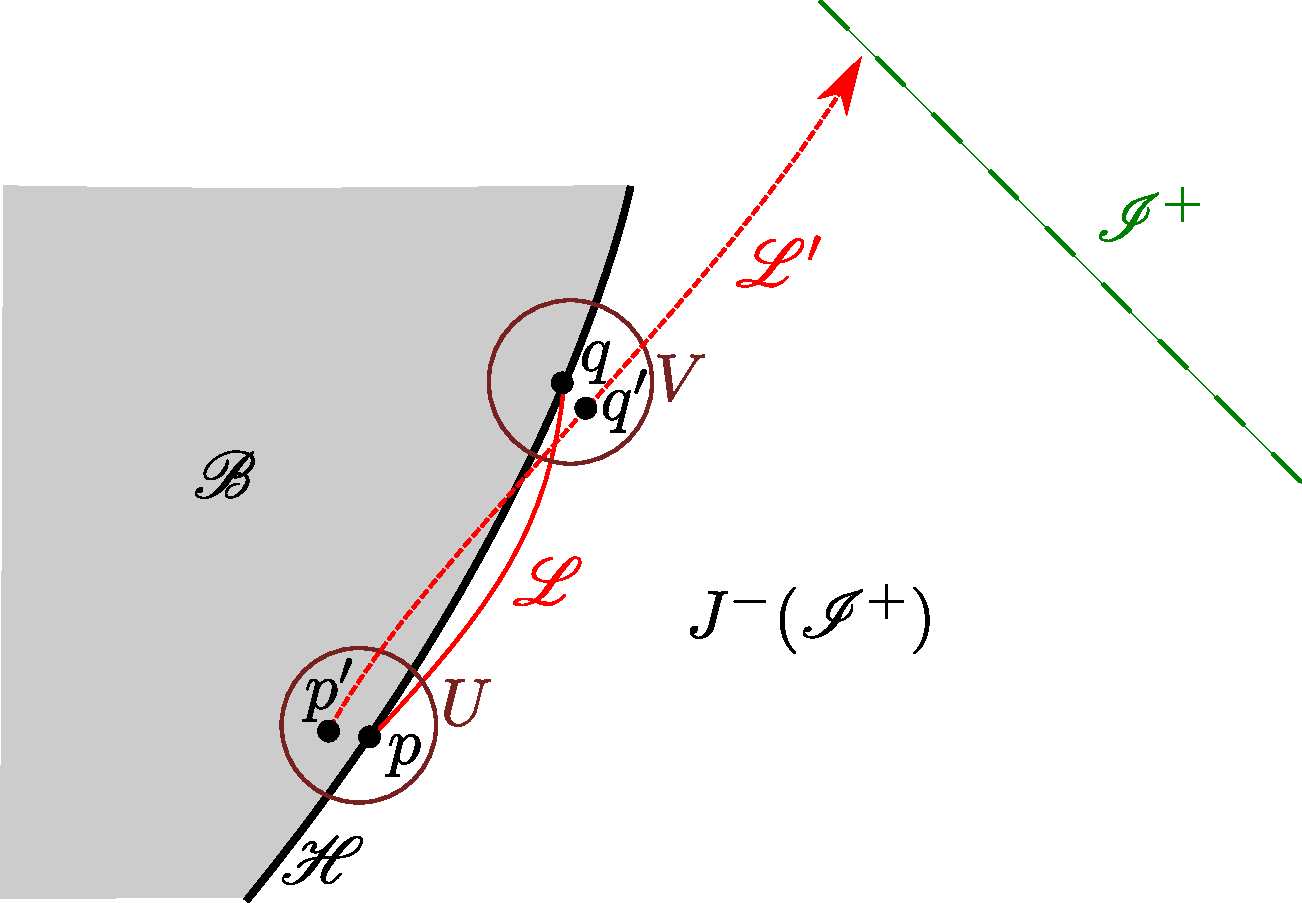
\includegraphics[width=0.55\textwidth]{glo_achronal.pdf}}
\caption[]{\label{f:glo:achronal} \footnotesize
Proving that $\Hor$ is achronal.}
\end{figure}

\begin{proof}
Let us assume the negation of Property~1, i.e. that there exists two points
in $\Hor$ which are connected by a timelike curve $\Li$. Let us call $p$ and
$q$ these two points, with $q$ in the future of $p$ (cf. Fig.~\ref{f:glo:achronal}).
We shall then use the following property:\\[1ex]
\textbf{Lemma 1}: One can ``move the ends'' of any timelike curve
``a little bit'' and still get a timelike curve. More precisely,
if two points $p,q\in\M$ are connected by a timelike curve,
there exists
a neighbourhood $U$ of $p$ and a neighbourhood $V$ of $q$ such that
any point $p'\in U$ can be connected to any point $q'\in V$ by a timelike curve.
\begin{proof}[Proof of Lemma 1]
This is more or less evident on a spacetime diagram (cf. Fig.~\ref{f:glo:timelike_stab})
and a formal proof
can be found as Lemma~3
in Chap.~14 of O'Neill's textbook \cite{ONeil83}.
\end{proof}
Applying Lemma~1,
let us choose $p'\in U\cap\mathscr{B}$ and $q'\in V\cap J^-(\scri^+)$. Such a choice is
always possible since $p$ and $q$ lie on the boundary between $\mathscr{B}$
and $J^-(\scri^+)$ (cf. Fig.~\ref{f:glo:achronal}).
Since $q'\in J^-(\scri^+)$, the timelike curve linking $p'$ and $q'$ can then be extended in the future into a causal curve $\Li'$ reaching $\scri^+$. This implies $p'\in J^-(\scri^+)$,
which contradicts $p'\in\mathscr{B}$.
\end{proof}

\begin{figure}
\centerline{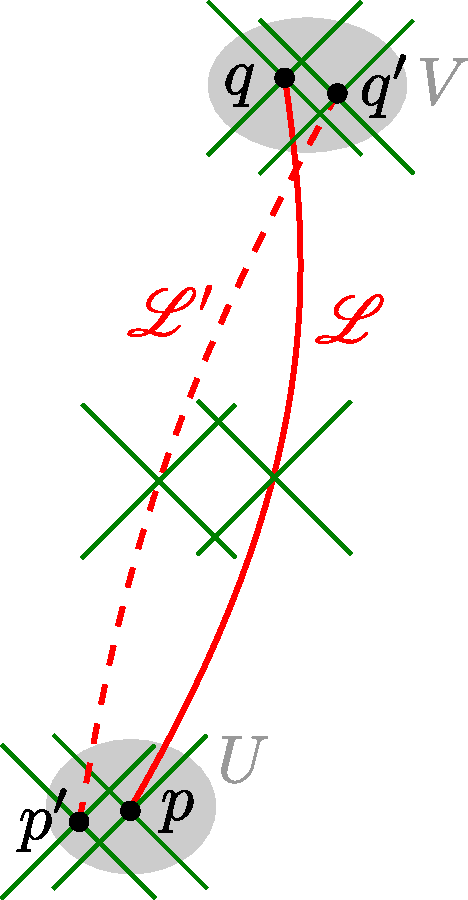
\includegraphics[height=0.3\textheight]{glo_timelike_stab.pdf}}
\caption[]{\label{f:glo:timelike_stab} \footnotesize
Lemma~1: moving slightly the ends $p$ and $q$ of a timelike curve $\Li$
yields another timelike curve $\Li'$.}
\end{figure}


\subsubsection{Property 2:}
\begin{greybox}
$\Hor$ is a topological manifold of dimension $n-1$, $n$ being the spacetime
dimension.
\end{greybox}

\begin{figure}
\centerline{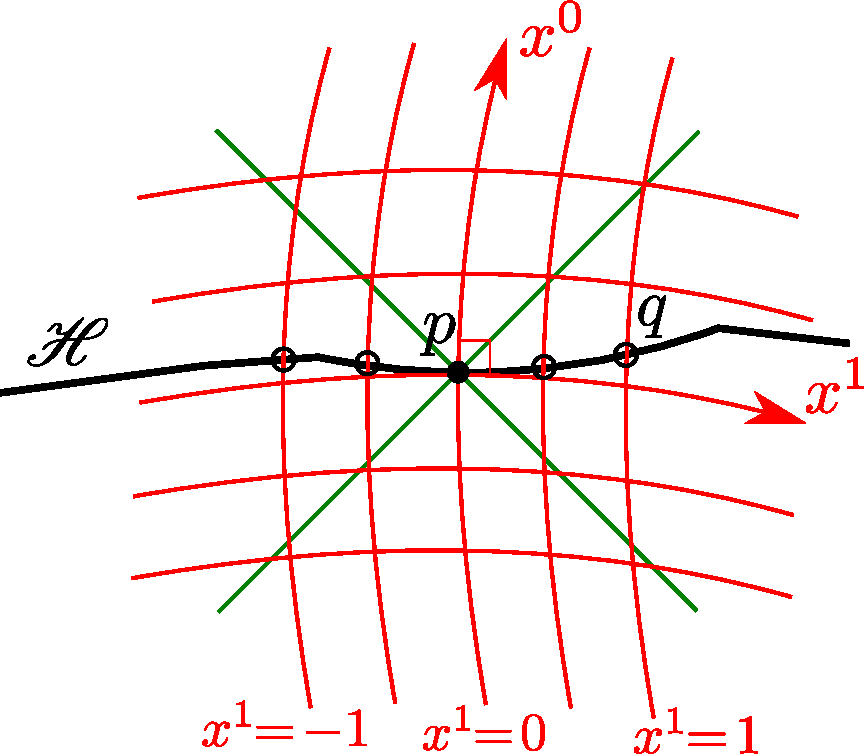
\includegraphics[width=0.45\textwidth]{glo_hor_manifold.pdf}}
\caption[]{\label{f:glo:hor_manifold} \footnotesize
Proving that $\Hor$ is a topological manifold of dimension $n-1$.}
\end{figure}

\begin{proof}
Let $p\in\Hor$ and $U$ some open neighbourhood of $p$ where one can define
a normal coordinate system $(x^\alpha)$. We have then $\wpar_0$ timelike,
$\wpar_i$ spacelike for $i\in\{1,\ldots,n-1\}$ and $\w{g}(\wpar_0, \wpar_i) = 0$.
Let us consider a curve in $U$ defined by $x^1 = a_1$,..., $x^{n-1} = a_{n-1}$,
where $a_1$, ..., $a_{n-1}$ are $n-1$ constants.
This curve is timelike, since it has $\wpar_0$ as a tangent vector
(cf. Fig.~\ref{f:glo:hor_manifold}).
It therefore intersects $\Hor$ at a single point $q$, for $\Hor$ is achronal (Property~1).
Let us then give the coordinates $(y^i) = (a_1,\ldots,a_{n-1})$ to $q$.
By varying $(a_1,\ldots,a_{n-1})$, we get a homeomorphism from $U\cap\Hor$
to an open subset of $\mathbb{R}^{n-1}$.
\end{proof}

\begin{remark}
Generically, the topological manifold $\Hor$ is not a smooth manifold, for it
contains some points (the crossovers defined below) at which it is not differentiable.
Actually $\Hor$ is slightly more than a mere topological submanifold of $\M$: it is a
\emph{Lipschitz submanifold} of $\M$. The latter is
intermediate between a topological submanifold, i.e.
a submanifold of class $C^0$ (continuous), and a differentiable submanifold of
class $C^1$. On $U\cap\Hor$, the function $x^0$ is a Lipschitz function
of the coordinates $(y^i)$: $\left|x^0(y^i) - x^0({y'}^i)\right| < K \sqrt{\sum_i (y^i - {y'}^i)^2}$.
This follows from the achronal character of $\Hor$: the points of coordinates
$(y^i)$ and $({y'}^i)$ cannot have a too large separation in terms of $x^0$,
otherwise they would be timelike separated.
Hence, one says that $\Hor$ is a \defin{Lipschitz submanifold}\index{Lipschitz submanifold} of $\M$. The notation $C^{1-}$ (i.e. a kind of intermediate between
$C^0$ and $C^1$) is generally used to denote Lipschitz submanifolds.
\end{remark}

\subsubsection{Property 3 (Penrose 1968 \cite{Penro68}):}
\begin{greybox}
$\Hor$ is ruled by a family of null geodesics that (i) either lie entirely
in $\Hor$ or at least never leave $\Hor$ when followed into the future from the
point where they arrived in $\Hor$, and
(ii) have no endpoint in the future.
Moreover, there is exactly one null geodesic through each point of $\Hor$,
except at special points where null geodesics enter in contact with $\Hor$, which are
called \defin{crossovers}\index{crossover point}. A special case
of crossover, called \defin{caustic}\index{caustic}, is a point
where neighbouring null geodesics focus and converge while entering on $\Hor$.
\end{greybox}
In particular, once a null geodesic has
merged with $\Hor$ (at a point where it may intersect other null geodesics),
it will stay forever on $\Hor$ and will never intersect any other null geodesic
of the family ruling $\Hor$. These null geodesics are called the
\defin{generators of}\index{generator!of an event horizon} $\Hor$.
The set of all crossovers is called the \defin{crease set}\index{crease set}
\cite{Siino98a,Siino98b,Brill14}.

\begin{figure}
\centerline{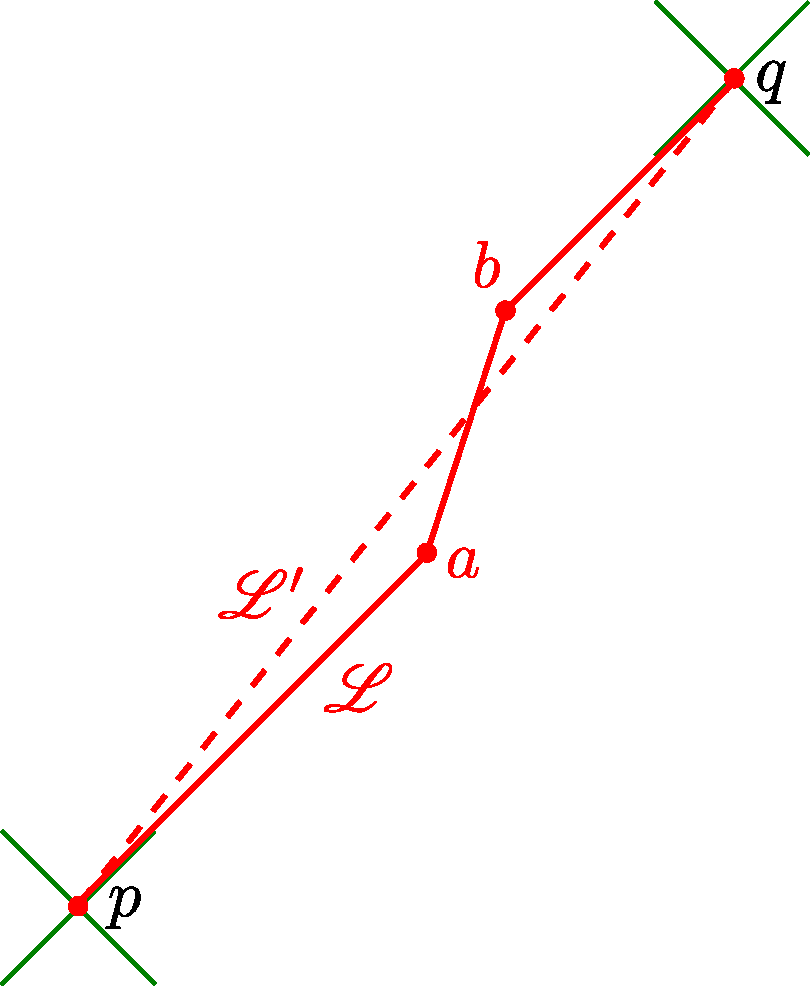
\includegraphics[width=0.3\textwidth]{glo_timelike_arc.pdf}}
\caption[]{\label{f:glo:timelike_arc} \footnotesize
Lemma 2: A \emph{causal} curve $\Li$ containing a timelike segment (between
$a$ and $b$ on the figure) can be deformed into a \emph{timelike} curve $\Li'$
with the ends kept fixed (dashed curve).}
\end{figure}


\begin{proof}
The following proof is adapted from that presented in Box~34.1 of MTW \cite{MisneTW73}.
It relies on the following lemma:\\[1ex]
\textbf{Lemma~2:} Let $\Li$ be a causal curve connecting two points $p$ and $q$
of $\M$. If $\Li$ contains a timelike segment, then there exists an
entirely timelike curve connecting $p$ and $q$.
\begin{proof}[Proof of Lemma 2]
We shall provide only a graphical ``proof'', based on the spacetime diagram
of Fig.~\ref{f:glo:timelike_arc}. The causal curve $\Li$ may have parts where it is null (segments $pq$ and $bq$ in Fig.~\ref{f:glo:timelike_arc}); these parts are drawn with
an angle of incline $\theta = \pm 45^\circ$.
If $\Li$ contains a timelike segment (as $ab$ in Fig.~\ref{f:glo:timelike_arc}), i.e. a segment with $|\theta|>45^\circ$,
it can be deformed, while keeping the same ends, to a curve with $|\theta|>45^\circ$
everywhere, i.e. to a timelike curve.
\end{proof}


\begin{figure}
\centerline{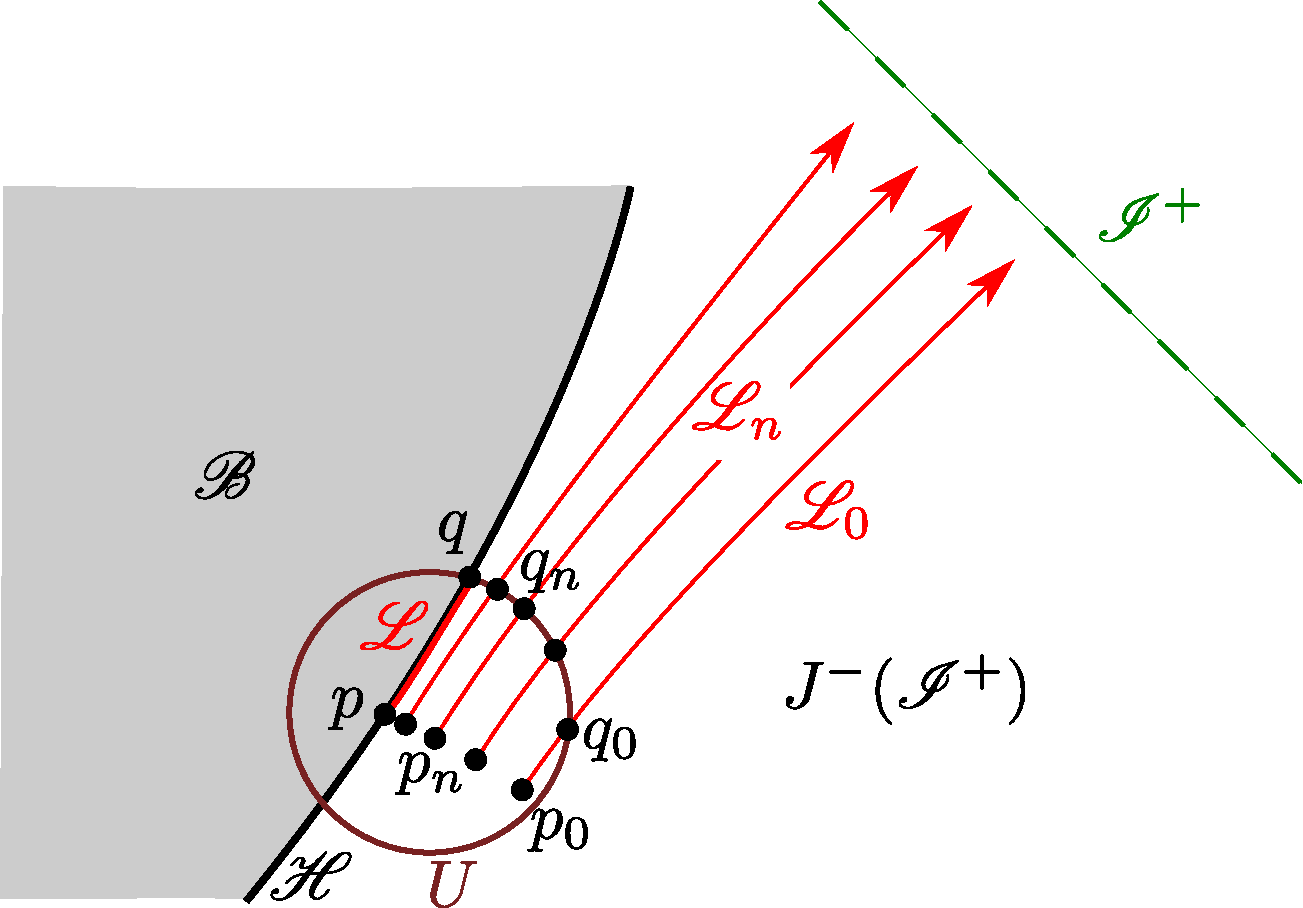
\includegraphics[width=0.55\textwidth]{glo_point_sequence.pdf}}
\caption[]{\label{f:glo:point_sequence} \footnotesize
Causal curve $\Li$ connecting $p$ to $q$ obtained as a limit of causal curves
in $J^-(\scri^+)$.}
\end{figure}


Let $p\in\Hor$ and let $U$ be some convex open neighbourhood of $p$.
Since $p$ lies in the boundary of $J^-(\scri^+)$, it is always possible to
consider
a sequence of points $(p_n)_{n\in\mathbb{N}}$ converging toward $p$
and such that $\forall n\in\mathbb{N},\ p_n \in U \cap J^-(\scri^+)$
(cf. Fig.~\ref{f:glo:point_sequence}).
Since $p_n\in J^-(\scri^+)$,
there exists a future-directed causal curve $\Li_{n}$ from $p_n$ to $\scri^+$
for each $n\in\mathbb{N}$.
The neighbourhood $U$ being convex, each $\Li_n$ intersects its boundary $\partial U$
at a unique point, $q_n$ say: $\{q_n\}=\Li_n \cap \partial U$
(cf. Fig.~\ref{f:glo:point_sequence}).
Since $\partial U$
is compact, the sequence $(q_n)_{n\in\mathbb{N}}$ admits a subsequence,
$(q_{f(n)})_{n\in\mathbb{N}}$ say ($f$ being an increasing
function $\mathbb{N}\rightarrow\mathbb{N}$),
that converges to some limit point $q$.
Since from any point $p_{f(n)}$ arbitrary close to $p$, there is
the causal curve $\Li_{f(n)}$ to the point $q_{f(n)}$ arbitrary close to $q$,
one can show that
there exists a causal curve $\Li$ connecting $p$ to $q$
(cf. Fig.~\ref{f:glo:point_sequence}; see e.g.
Lemma~6.2.1 of Hawking \& Ellis textbook \cite{HawkiE73}
for a precise demonstration).

As the limit of points in $J^-(\scri^+)$, $q$ lies in the closure
$\overline{J^-(\scri^+)} = J^-(\scri^+) \cup \Hor$, $\Hor$
being the boundary of $J^-(\scri^+)$.
Let us show by contradiction that actually $q\in\Hor$.
If we assume $q\not\in\Hor$, then necessarily $q\in J^-(\scri^+)$.
There exists then an open neighbourhood $V$ of $q$ such that $V \subset  J^-(\scri^+)$
(cf. Fig.~\ref{f:glo:q_in_H}).
Let us choose $q'\in V$ such that $q$ is connected to $q'$ via a timelike curve.
We may then extend $\Li$ to a causal curve $\tilde{\Li}$ from $p$ to $\scri^+$
via $q$ and $q'$ (cf. Fig.~\ref{f:glo:q_in_H}). Since $\tilde{\Li}$ contains a timelike segment
(between $q$ and $q'$), we may invoke Lemma~2 to deform it into
a timelike curve $\tilde{\Li}'$ between $p$ and $\scri^+$. Then, by Lemma~1,
one can ``move the past end'' of $\tilde{\Li}'$
to get a new timelike curve $\tilde{\Li}''$ linking an event $p'\in\mathscr{B}$ close
to $p$ to $\scri^+$ (dotted curve in Fig.~\ref{f:glo:q_in_H}), which is impossible by the very definition of the black hole
region $\mathscr{B}$. Hence we have that $q\in\Hor$.

\begin{figure}
\centerline{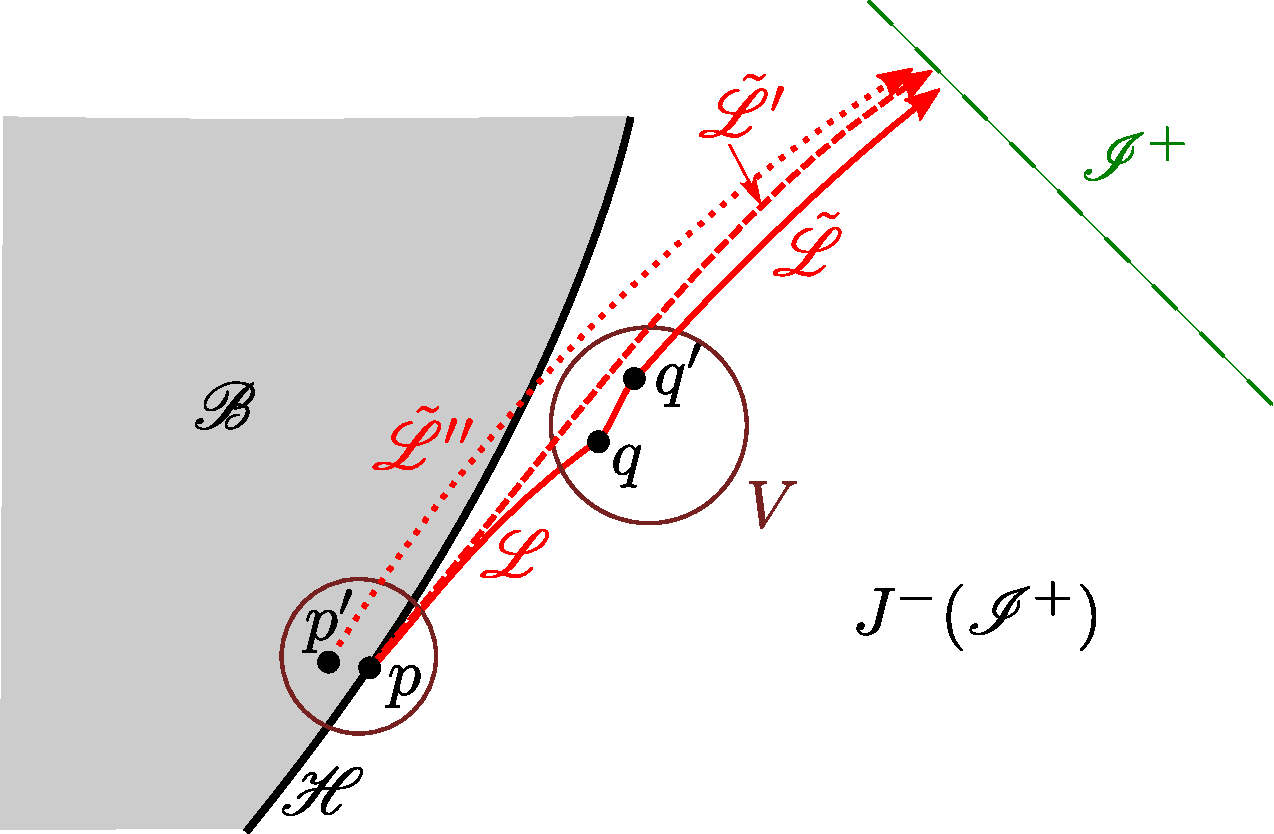
\includegraphics[width=0.55\textwidth]{glo_q_in_H.pdf}}
\caption[]{\label{f:glo:q_in_H} \footnotesize
Proving by contradiction that $q$ lies in $\Hor$.}
\end{figure}


The causal curve $\Li$ connecting $p$ to $q$ cannot be timelike since
$p$ and $q$ are both in $\Hor$, which is achronal (Property~1).
If $\Li$ would contain a timelike segment, then by Lemma~2, it could
be deformed into a timelike curve between $p$ and $q$, which again would
contradict the achronal character of $\Hor$. Hence $\Li$ is necessarily a null
curve. If it would not be a null geodesic, it would not have an extremum length
between all curves connecting $p$ and $q$ (the length being defined as
the integral of the scalar square $\D s^2 = \w{g}(\D\w{x}, \D\w{x})$
of the displacement vector $\D\w{x}$ along the curve).
The length of $\Li$ being zero, there would then exist some curves of negative
length connecting $p$ and $q$. Since such curves are timelike, this
would be in contradiction with the achronal character of $\Hor$.

At this stage, we have shown that given $p\in\Hor$, there exists
a future-directed null geodesic $\Li$ connecting $p$ to another point $q\in\Hor$.
There remains to show that $\Li$ lies entirely in $\Hor$.
Let us start by showing that $\Li\subset \overline{J^-(\scri^+)}$.
Let $a$ be a generic point of $\Li$ between $p$ and $q$. Since $\Li$ is
null, there exists a point
$a'$ arbitrary close to $a$ such that $a'$ is connected to $q$ by a
future-directed timelike curve (cf. Fig.~\ref{f:glo:L_in_H}). Thanks to Lemma~1
and the property $q\in \overline{J^-(\scri^+)}$, we may
find a point $q'\in J^-(\scri^+)$ close to $q$ such that $a'$ is connected
to $q'$ by a future-directed timelike curve.
Since $q'\in J^-(\scri^+)$, such a curve can be extended
to a causal curve to $\scri^+$  (the dashed curve
in Fig.~\ref{f:glo:L_in_H}); hence
$a'\in  J^-(\scri^+)$. Since $a'$ is arbitrary close to $a$, we conclude
that $a\in\overline{J^-(\scri^+)}$.
This property being valid for any point $a\in \Li$, we have
shown in fact that $\Li\subset \overline{J^-(\scri^+)} = J^-(\scri^+)\cup \Hor$.
Now it is easy to show that any point $a$ of $\Li$ actually lies in $\Hor$
by repeating exactly the same reasoning as that employed above to show that
$q\in\Hor$, by replacing $q$ by $a$. We therefore conclude that
$\Li$ lies entirely in $\Hor$.

\begin{figure}
\centerline{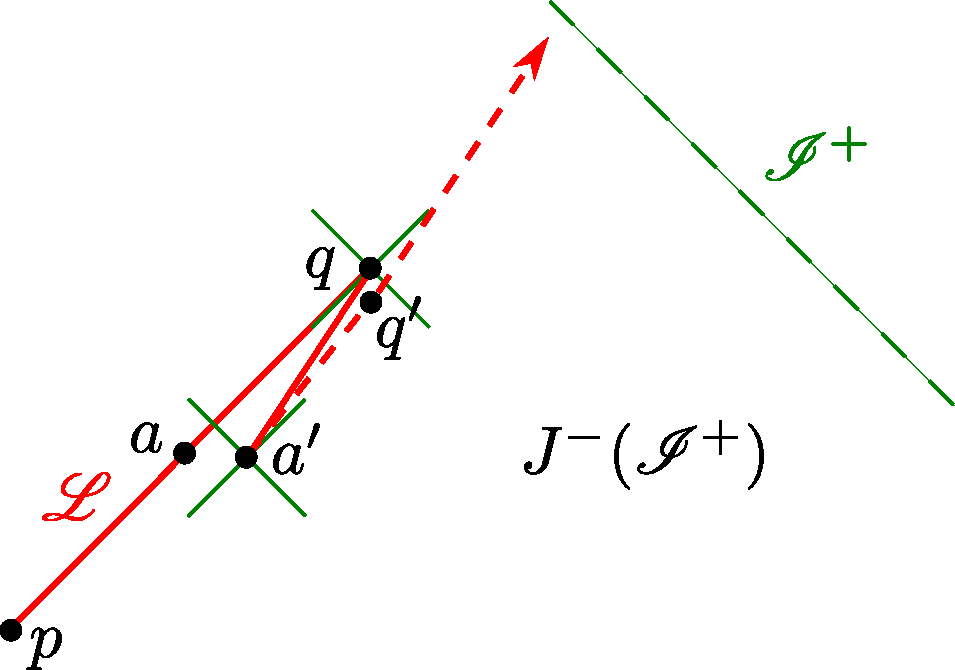
\includegraphics[width=0.45\textwidth]{glo_L_in_H.pdf}}
\caption[]{\label{f:glo:L_in_H} \footnotesize
Proving that $\Li$ lies entirely in $\Hor$.}
\end{figure}



Given a point $p\in\Hor$, we have thus constructed a
future-directed null geodesic $\Li$ lying entirely in $\Hor$ and
connecting $p$ to another point $q\in\Hor$. One can
repeat the construction
from the point $q$ to get another future-directed null geodesic $\Li'\subset\Hor$
connecting $q$ to another point $q'\in\Hor$. Now $\Li$ and $\Li'$ must
be two segments of the same null geodesic $\Li\cup\Li'$ by the following lemma:\\[1ex]
\textbf{Lemma~3}: If from a point $q\in\Hor$, there exists a past-directed
null geodesic $\Li\subset\Hor$ and a future-directed null geodesic $\Li'\subset\Hor$,
then necessarily $\Li$ and $\Li'$ have collinear tangent vectors at their common point $q$.
It follows that $\Li$ (with a time-reversed parametrization) and $\Li'$ are two segments
of a same null geodesic through $q$.
\begin{figure}
\centerline{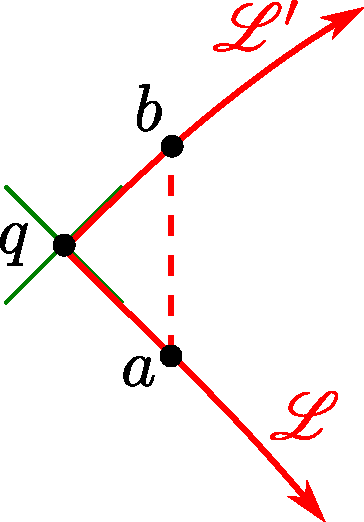
\includegraphics[width=0.17\textwidth]{glo_unique_geod.pdf}}
\caption[]{\label{f:glo:unique_geod} \footnotesize
Proof of Lemma~3.}
\end{figure}
\begin{proof}[Proof of Lemma 3]
Assume that $\Li$ and $\Li'$ have non-collinear tangent vectors at $q$. Then, in
the vicinity of $q$, one can find a point $a\in\Li$ and a point $b\in\Li'$
such that $a$ and $b$ can be connected by a timelike curve (cf.
Fig.~\ref{f:glo:unique_geod}). Since $\Li\subset\Hor$ and $\Li'\subset\Hor$, we have $a\in\Hor$ and
$b\in\Hor$ and therefore we get a contradiction with $\Hor$ being achronal.
\end{proof}
Thanks to Lemma~3, we conclude that $\Li'$ extends $\Li$ to null geodesic
$\Li\cup\Li'$ entirely lying in $\Hor$. By iterating, we conclude that
the null geodesic $\Li$ through $p$ can be extended indefinitely into the
future. Moreover, it can never leave $\Hor$. Indeed, if it leaves $\Hor$ at
some point $q$, by the same procedure used above for $p$, one could construct a future-directed null geodesic
$\Li'\subset\Hor$ starting from $q$ and Lemma~3 would imply that
the extension of $\Li$ outside $\Hor$ has to coincide with $\Li'$, which is
in contradiction with $\Li'\subset\Hor$.

Another direct consequence of Lemma~3 is that no two distinct null generators
may intersect at a point $p\in\Hor$, except if their segments in the past of
$p$ lie outside $\Hor$.
This completes the proof of Property~3.
\end{proof}


\begin{figure}
\centerline{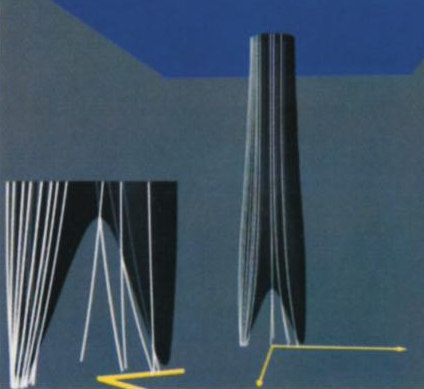
\includegraphics[width=0.5\textwidth]{glo_BH_headon_gener.jpg}}
\caption[]{\label{f:glo:BH_headon_gener} \footnotesize
Spacetime diagram of the event horizon corresponding to the head-on merger of
two black holes as computed by Matzner et al. (1995) \cite{Matzn_al95}. The
white curves are some null geodesic generators; the left picture is a zoom of
the merger region, with the crease set
(source: Fig.~4 of Ref.~\cite{Matzn_al95}; \copyright 1995 American Association for the Advancement of Science).}
\end{figure}



Some features of Property~3 are illustrated in Fig.~\ref{f:glo:BH_headon_gener},
which displays the null geodesic generators in a numerical simulation
of the head-on collision of two black holes by Matzner et al. (1995) \cite{Matzn_al95}.
Note that new null geodesics enter in the event horizon at the ``crotch'' of the
``pair of pants''.

The head-on black hole merger has been also computed by Cohen et al. (2009) \cite{CohenPS09}, with an increase numerical accuracy (cf. Fig.~\ref{f:glo:EH_headon_3d}).
Cross-sections of the event horizon $\Hor$ (cf. Sec.~\ref{s:def:spacelike_sections})
are depicted in Fig.~\ref{f:glo:EH_headon}. The same figure shows also how
some null geodesics will reach $\Hor$ to become null generators.


\begin{figure}
\centerline{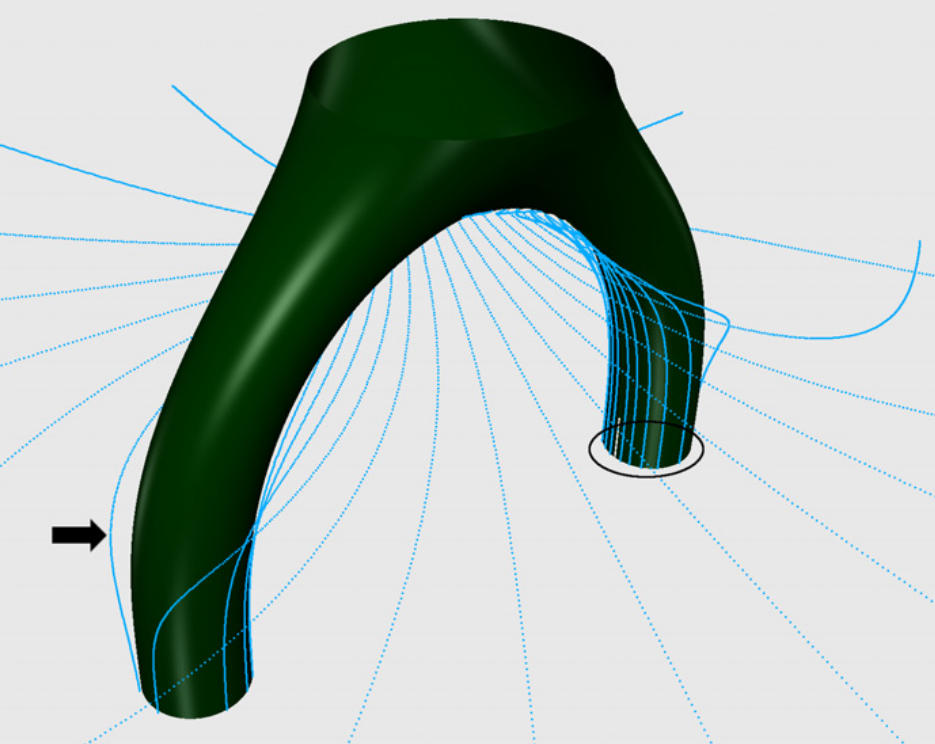
\includegraphics[width=0.5\textwidth]{glo_EH_headon_3d.jpg}}
\caption[]{\label{f:glo:EH_headon_3d} \footnotesize
Spacetime diagram of the event horizon corresponding to the head-on merger of
two black holes as computed by Cohen et al. (2009) \cite{CohenPS09}.
The blue curves are null geodesics that will eventually become null generators
of the event horizon; those arising from regions close to the event horizon
are marked by the arrow and the black ellipse
(source: Fig.~15 of Ref.~\cite{CohenPS09}; \copyright 2009 IOP Publishing Ltd).}
\end{figure}

\begin{figure}
\centerline{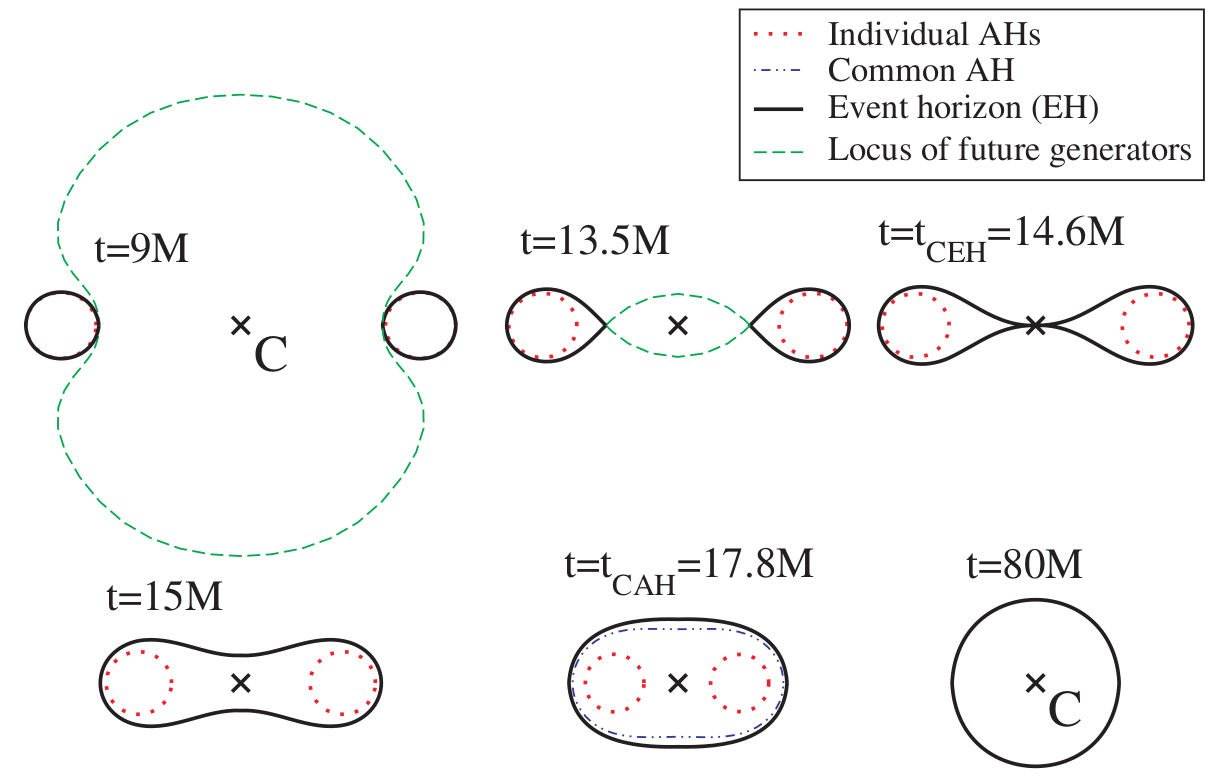
\includegraphics[width=0.8\textwidth]{glo_EH_headon.jpg}}
\caption[]{\label{f:glo:EH_headon} \footnotesize
Cross-sections (at various coordinate time $t$) of the event horizon $\Hor$ corresponding
to the head-on merger of two black holes as computed by Cohen et al. (2009) \cite{CohenPS09}
and displayed in Fig.~\ref{f:glo:EH_headon_3d}.
Each figure is a 2D cut of a hypersurface $\Sigma_t$ defined by a constant
value of the coordinate time $t$, expressed in units of the sum $M$ of the initial irreducible masses of each black
hole (cf. Sec.~??). The whole 3D hypersurface $\Sigma_t$ can be reconstructed
by rotation around the collision axis.
$t_{\rm CEH}$ (for ``Common Event Horizon'')
is the coordinate time at which the cross-section of $\Hor$ becomes a connected
2-surface.
The cross-sections of $\Hor$ are displayed
in black, while the green dashed curves denote the set of the intersections
with $\Sigma_t$ of the null geodesics that
will become null generators $\Hor$ through the cusps in the
``individual'' event horizons.
The red and blue dashed curves denotes apparent horizons (cf. Sec.~??).
(source: Fig.~1 of Ref.~\cite{CohenPS09}; \copyright  2009 IOP Publishing Ltd).}
\end{figure}

Finally, Fig.~\ref{f:glo:EH_binspir} shows a cross-section
of the event horizon computed by Cohen et al. (2012) \cite{CohenKS12}
in some inspiralling binary black hole merger. The
black hole spacetime itself has been computed as a solution of the vaccum
Einstein equation by Scheel at al. \cite{ScheeBCKMP09}; it corresponds to
16 inspiralling orbits of a equal-mass binary black hole with vanishing initial
spins.

\begin{figure}
\centerline{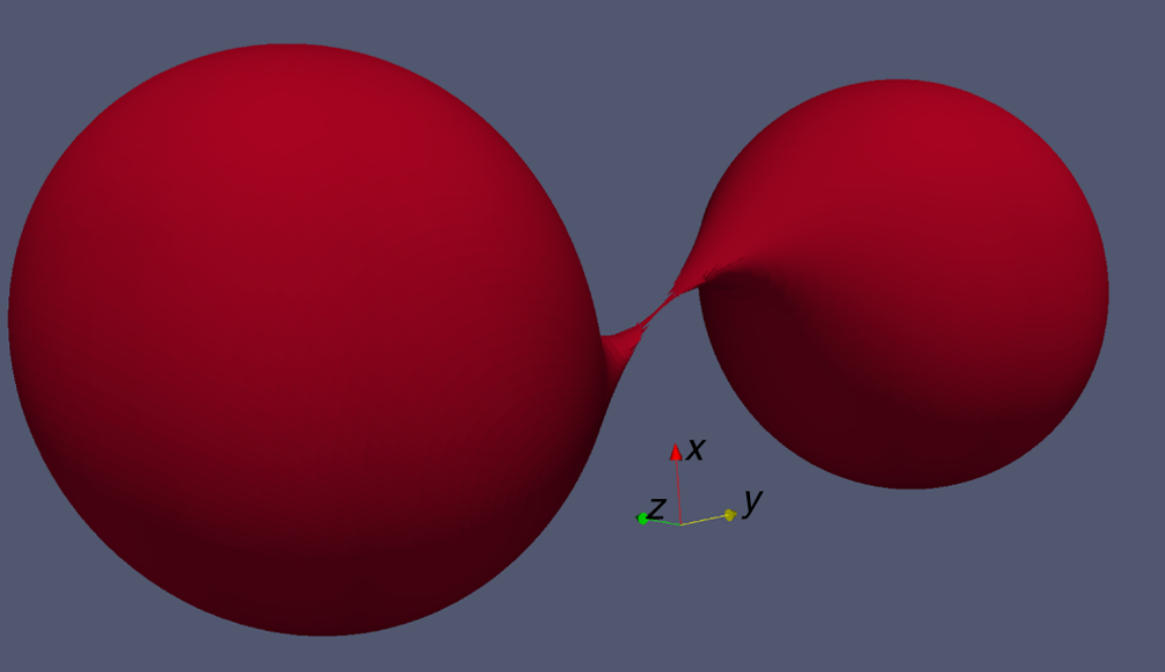
\includegraphics[width=0.6\textwidth]{glo_EH_binspir.jpg}}
\caption[]{\label{f:glo:EH_binspir} \footnotesize
Cross-section of the event horizon $\Hor$ of the inspiralling merger of
two black holes as computed by Cohen et al. (2012) \cite{CohenKS12}.
The $x$ and $y$ axes define the orbital plane.
This cross-section is the first connected one in the slicing of $\Hor$
by surfaces of constant coordinate time $t$
(source: Fig.~2 of Ref.~\cite{CohenKS12}; \copyright 2012 American Physical Society).}
\end{figure}

Generically, for a binary black hole merger,
the crease set forms a 2-dimensional subset of the event horizon
$\Hor$ and is bounded by the set of caustic points, which forms a 1-dimensional
subset of $\Hor$ \cite{Siino98a,Siino98b,HusaW99,CohenKS12}.

\subsubsection{Property 4:}
\begin{greybox}
Wherever it is smooth, $\Hor$ is a null hypersurface.
\end{greybox}
\begin{proof}
Let us assume that $\Hor$ is smooth in some open subset $U$.
By Property~2, $\Hor$ is then a smooth hypersurface in $U$.
According to Property~3, there is a null geodesic lying in $\Hor$ through
any point of $\Hor\cap U$.
This implies null tangent vectors at any point of $\Hor\cap U$, so that, in $U$,
$\Hor$ must be either a null hypersurface or a timelike one. But $\Hor$ is achronal by Property~1 and therefore cannot be timelike. Hence $\Hor$ is a null hypersurface in $U$.
\end{proof}
When $\Hor$ is smooth, its generators,
as defined in Property~3, are then nothing but the
null-hypersurface generators as defined in Sec.~\ref{s:def:geod_gener}.

\begin{remark}
Properties 1 to 4 are not specific to black hole horizons: they are actually
valid for any boundary $\partial J^-(S)$ of the causal past of a given set $S\subset\M$.
They are also valid for the boundary $\partial J^+(S)$ of the causal future of
$S$, modulo the relevant changes future $\leftrightarrow$ past in Property~3.
\end{remark}

It can be shown that event horizons are smooth almost everywhere: the only
location where they are not differentiable is the crease set, i.e. the set of points
where null geodesics cross each other while arriving at $\Hor$ and becoming null
generators.

%%%%%%%%%%%%%%%%%%%%%%%%%%%%%%%%%%%%%%%%%%%%%%%%%%%%%%%%%%%%%%%%%%%%%%%%%%%%%%%%%%%%%%%%

  % The concept of black hole 3: The global view

\chapter{Stationary black holes}
\label{s:sta}

\minitoc

\section{Introduction}

\section{Definition and first properties} \label{s:sta:def_station}

Let us consider a spacetime $(\M,\w{g})$ that contains a black hole, as defined in
Sec.~\ref{s:glo:def_BH}. In particular, $(\M,\w{g})$ admits a future null
infinity $\scri^+$ and a past null infinity $\scri^-$. One says that
$(\M,\w{g})$ is a \defin{stationary spacetime}\index{stationary!spacetime}
if (i) it is invariant under
the action of the translation group $(\mathbb{R},+)$ and (ii) the orbits of
the group action are timelike curves in the vicinity of $\scri^+$ and
$\scri^-$. It is equivalent to say that there exists a Killing vector field
$\w{\xi}$ (the generator of the translation group, cf. Sec.~\ref{s:neh:symmetries}) that is timelike in the vicinity of $\scri^+$ and $\scri^-$.

\begin{remark}
Some authors (e.g. Carter \cite{Carte73b}) call such spacetimes
\emph{pseudo-stationary}\index{pseudo-stationary}, keeping the qualifier
\emph{stationary} for the case where the Killing field $\w{\xi}$ is timelike
in all $\M$. As we going to see, when $\M$
contains a black hole, $\w{\xi}$ cannot be timelike everywhere,
so only \emph{pseudo-stationarity} in the above sense is relevant for them.
Our terminology follows that of Chru\'sciel, Lopes Costa \& Heusler \cite{ChrusLH12}
and Choquet-Bruhat \cite{Choqu09}.
\end{remark}

If $(\M,\w{g})$ is invariant under the action of the isometry group $(\mathbb{R},+)$,
so is $\scri^+$ (under some proper extension of $\w{\xi}$ to the conformal
completion $\tilde{\M}$)
and therefore its causal past $J^-(\scri^+)$. As the boundary of $J^-(\scri^+)$
inside $\M$, the event horizon $\Hor$ must therefore be invariant under the
action of the isometry group.
Note that this means that $\Hor$ is invariant \emph{as a whole}, not that
each point of $\Hor$ is invariant under the group action.
Now, $\Hor$ is globally invariant if, and only if, the
generator $\w{\xi}$ of the isometry group is tangent to $\Hor$.
Let us assume that $\Hor$ is smooth (which sounds likely in a stationary context;
a rigorous proof can be found in \cite{ChrusDGH01}),
it is then a null hypersurface (Property~4 in Sec.~\ref{s:glo:properties_H}).
Since a timelike vector cannot be tangent to a null hypersurface (cf. the
lemma in Sec.~\ref{s:def:spacelike_sections}), we conclude that
\begin{greybox}
In a stationary spacetime containing a black hole,
the stationary Killing vector field  $\w{\xi}$ is tangent to the event horizon
$\Hor$, which implies that $\w{\xi}$ is either null or spacelike on $\Hor$.
\end{greybox}

\section{The event horizon as a Killing horizon}

Let us discuss successively the two allowed types for the stationary
Killing vector $\w{\xi}$ on $\Hor$: null and spacelike.

\subsection{Null stationary Killing field on $\Hor$: the staticity theorem}

By the lemma of Sec.~\ref{s:def:spacelike_sections}, if the Killing vector
field $\w{\xi}$ is null on $\Hor$, it is necessarily tangent to the null geodesic generators
of $\Hor$ and therefore collinear to the null normals $\wl$ of $\Hor$. From the definition
given in Sec.~\ref{s:neh:def_Killing_hor}, it follows immediately that
$\Hor$ is a Killing horizon (with respect to the Killing field $\w{\xi}$).
In dimension $n=4$ and using the Einstein equation,
D.~Sudarski and R.M.~Wald (1992) \cite{SudarW92} have then proven that $\w{\xi}$ must be
hypersurface-orthogonal everywhere, i.e. that the spacetime $(\M,\w{g})$ is \defin{static}\index{static spacetime}. For this reason, Sudarski \& Wald's result is often
called the \defin{staticity theorem}\index{staticity theorem}.

Having that $(\M,\w{g})$ is static, we can go further and
apply the
\begin{greybox}[frametitle={Israel uniqueness theorem:}]
\index{Israel uniqueness theorem}
If $(\M,\w{g})$ is a $n$-dimensional static spacetime
containing a black hole, with $\w{g}$ solution of the vacuum Einstein
equation, then the domain of outer communications of $\M$ is isomorphic
to the domain of outer communications of a $n$-dimensional Schwarzschild spacetime\index{Schwarzschild!spacetime}.
\end{greybox}
This theorem has been proved in 1967 by W.~Israel \cite{Israe67},
and improved latter by many authors (in particular by
P. Chru\'sciel \& G. Galloway (2010) \cite{ChrusG10}, who removed
the hypothesis of analyticity).
A demonstration of Israel's theorem can be found in Straumann's textbook \cite{Strau04}.

So basically, in dimension $n=4$ (i.e. when the staticity theorem applies), all stationary vacuum black holes with the stationary Killing field $\w{\xi}$ null
on $\Hor$ are nothing but Schwarzschild black holes, which we will study in detail in Chap.~\ref{s:sch}.


\subsection{Spacelike stationary Killing field on $\Hor$: the strong rigidity theorem}
\label{s:sta:strong_rigidity}

When $\w{\xi}$ is spacelike on $\Hor$, it obviously cannot be collinear to
any null normal $\wl$ of $\Hor$.
Assuming that $\Hor$ has cross-sections of spherical topology, we observe
that, with respect to the null geodesic generators of $\Hor$, the field lines of $\w{\xi}$
form some helices (cf. Fig.~??). By reciprocity, with respect to the field lines of $\w{\xi}$,
the null geodesic generators form some helices as well (cf. Fig.~??).
Since asymptotically the field lines of $\w{\xi}$ are worldlines of inertial observers,
we may say (in loose terms at this stage) that the event horizon $\Hor$
``is rotating'', all the more that we have seen above that when the null
generators coincide with the field lines of $\w{\xi}$, the black hole is static, i.e. non-rotating.

Since the Killing field $\w{\xi}$ is not null on $\Hor$, we cannot say a priori
that $\Hor$ is a Killing horizon. However, it turns out
that this is indeed the case, according to a famous result by S.W.~Hawking (1972)
\cite{Hawki72,HawkiE73}, known as the
\defin{strong rigidity theorem}\index{strong!rigidity theorem}\index{rigidity theorem!strong --}.
Assuming $n=4$ and the metric $\w{g}$ obeying the vacuum Einstein equation,
Hawking was able to show that there exists a second Killing vector field,
$\w{\chi}$ say, which is null on $\Hor$. Hence $\Hor$ is a Killing horizon
in this case as well, albeit not with respect to the
stationary Killing vector field $\w{\xi}$.

Hawking's result has been extended to dimensions $n\geq 4$ by V.~Moncrief
and J.~Isenberg (2008) \cite{MoncrI08}, under the hypotheses that $\Hor$
has cross-sections that are compact and transverse to $\w{\xi}$ (see also
Theorem~8.1 p.~470 of Choquet-Bruhat's textbook \cite{Choqu09}).
Both Hawking's result
and Moncrief \& Isenberg's one rely on the rather strong assumption that $\M$ and $\Hor$
are (real) \emph{analytic} manifolds, with $\w{g}$ being an analytic field. On physical grounds,
it would be desirable to assume only \emph{smooth} manifolds and fields.
Recently, S.~Alexakis, A.D.~Ionescu and S.~Klainerman \cite{AlexaIK14} (2014)
have succeeded in proving the strong rigidity theorem without the analyticity
assumption, but only for slowly rotating black holes.

Since we have two Killing vectors, $\w{\xi}$ and $\w{\chi}$, we may
form any linear combination of them with constant coefficients
and still get a Killing vector. For instance, if $\Omega_H$ is a non-zero constant,
the vector field $\w{\eta}$ defined by
\be
    \w{\eta} = \frac{1}{\Omega_H} \left( \w{\chi} - \w{\xi} \right)
    \quad\iff\quad
    \w{\chi} = \w{\xi} + \Omega_H \w{\eta} ,
\ee
is a Killing vector field on $\M$.
One can show (see e.g. \cite{Chrus97} for a rigorous proof) that $\Omega_H$
and some constant rescaling of $\w{\chi}$
can be chosen so that $\w{\eta}$ is a spacelike vector field whose
field lines are closed, with $2\pi$-periodicity in terms of the parameter $\ph$
associated to $\w{\eta}$ (i.e. $\w{\eta} = \D/\D\ph$ along the field lines),
and such that $\w{\eta}$ vanishes on a timelike 2-dimensional surface, called
the \defin{rotation axis}\index{rotation!axis}.
It follows that
the isometry group whose generator is $\w{\eta}$ is the rotation group
$\mathrm{SO}(2)$. In other words, the spacetime $(\M,\w{g})$ is
\defin{axisymmetric}\index{axisymmetric!spacetime} in addition to be stationary.
The constant $\Omega_H$ is then called the
\defin{black hole rotation velocity}\index{black hole!rotation velocity}\index{rotation!velocity}.

By the very definition of stationarity, the Killing vector field $\w{\xi}$ is
timelike in the vicinity of $\scri^+$ and $\scri^-$. If $\w{\xi}$ is spacelike
on $\Hor$, as assumed in this section, by continuity it must be spacelike
in some part of the domain of outer communications $\langle\langle \M\rangle\rangle$
near $\Hor$. The simplest configuration is then when
$\w{\xi}$ is spacelike in some connected region $\mathscr{G}\subset \langle\langle \M\rangle\rangle$
around $\Hor$, null at the boundary of $\mathscr{G}$ and timelike outside $\mathscr{G}$
up to $\scri^+$ and $\scri^-$ (cf. Fig.~??). The subset $\mathscr{G}$ is
called the \defin{ergoregion}\index{ergoregion} and its boundary $\E:=\partial\mathscr{G}$
the \defin{ergosphere}. We shall discuss it further in connection with
the Penrose process in Chap.~\ref{s:ker}.

%%%%%%%%%%%%%%%%%%%%%%%%%%%%%%%%%%%%%%%%%%%%%%%%%%%%%%%%%%%%%%%%%%%%%%%%%%%%%%%


\section{Bifurcate Killing horizons} \label{s:sta:bifur_Killing_hor}

\subsection{Definition and first properties}

Let $(\M,\w{g})$ be a $n$-dimensional spacetime endowed with a Killing vector
field $\w{\xi}$. A
\defin{bifurcate Killing horizon}\index{bifurcate!Killing horizon}\index{Killing!horizon!bifurcate --}\index{horizon!bifurcate Killing --} is the
union
\be
    \Hor = \Hor_1 \cup \Hor_2 ,
\ee
with the following properties:
\begin{itemize}
\item $\Hor_1$ and $\Hor_2$ are two null hypersurfaces;
\item $\Sp:=\Hor_1\cap\Hor_2$ is a spacelike $(n-2)$-surface;
\item each of the sets $\Hor_1\setminus\Sp$ and $\Hor_2\setminus\Sp$ has two connected components, which are
Killing horizons\footnote{Cf. Sec.~\ref{s:neh:def_Killing_hor} for the
definition of a Killing horizon.} with respect to $\w{\xi}$.
\end{itemize}
The $(n-2)$-dimensional submanifold $\Sp$ is called the
\defin{bifurcation surface}\index{bifurcation!surface} of $\Hor$.

\begin{figure}
\centerline{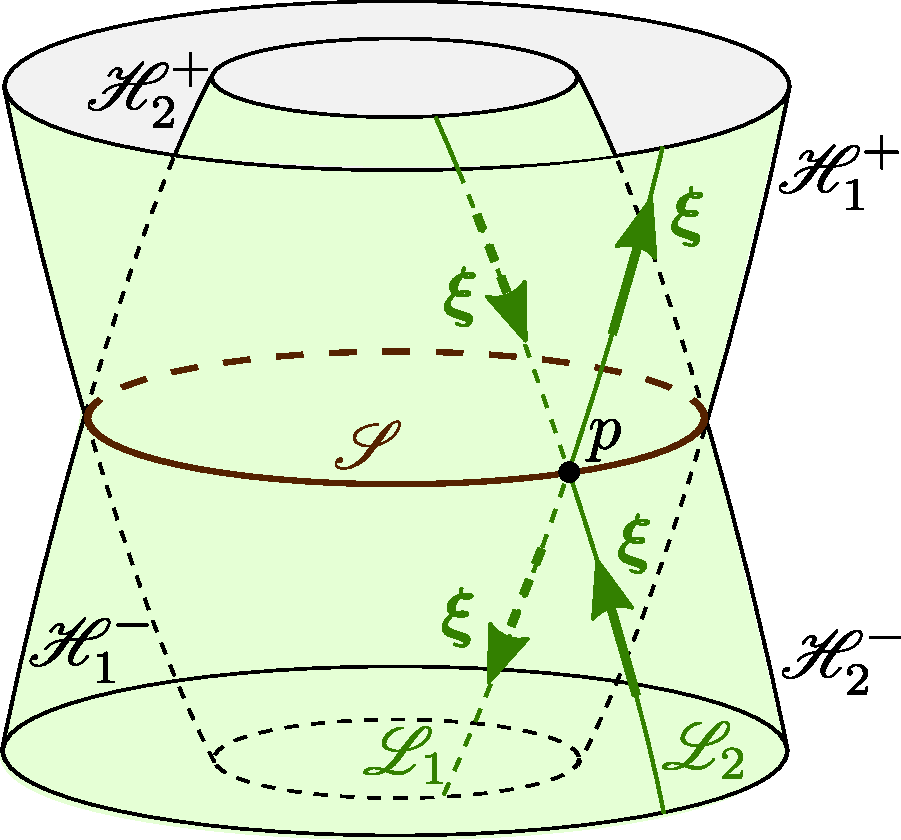
\includegraphics[width=0.5\textwidth]{sta_bifur_Kill_hor.pdf}}
\caption[]{\label{f:sta:bifur_Kill_hor} \footnotesize
Bifurcate Killing horizon $\Hor_1\cup\Hor_2$ with respect to the Killing vector
field $\w{\xi}$; $\Sp$ is the bifurcation surface. $\Li_1$ and $\Li_2$ are
null geodesic generators of respectively $\Hor_1$ and $\Hor_2$, which cross
each other at the point $p\in\Sp$.}
\end{figure}

Hence we may say that a bifurcate Killing horizon is formed by four Killing horizons,
$\Hor_1^+$, $\Hor_1^-$, $\Hor_2^+$ and $\Hor_2^-$ say,
which are merged together at the bifurcation surface $\Sp$ (cf. Fig.~\ref{f:sta:bifur_Kill_hor}), in such a way that
\[
    \Hor_1 = \Hor_1^- \cup \Sp \cup \Hor_1^+ \quad \mbox{and}\quad
    \Hor_2 = \Hor_2^- \cup \Sp \cup \Hor_2^+
\]
are null hypersurfaces.

A first property of bifurcate Killing horizons is
\begin{greybox}
The Killing vector field vanishes at the bifurcation surface:
\be
    \encadre{\left. \w{\xi} \right| _{\Sp} = 0 } .
\ee
\end{greybox}
\begin{proof}
Let $p\in \Sp$ and let us assume that $\left.\w{\xi}\right| _p\not=0$.
Let $\Li_1$ (resp. $\Li_2$) be the null geodesic generator of $\Hor_1$
(resp. $\Hor_2$) that intersects $\Sp$ at $p$ (cf. Fig.~\ref{f:sta:bifur_Kill_hor}).
Since $\Sp$ is spacelike,
$\Li_1$ and $\Li_2$ are unique. By definition of a Killing horizon,
$\w{\xi}$ is tangent to $\Li_1\cap\Hor_1^+$ and to $\Li_1\cap\Hor_1^-$,
i.e. to $\Li_1\setminus\{p\}$.
If $\left.\w{\xi}\right| _p \not=0$, then by continuity,
$\w{\xi}$ is a (non-vanishing) tangent vector field all along $\Li_1$.
Similarly, $\w{\xi}$ is tangent to all $\Li_2$.
At their intersection point $p$, $\Li_1$ and $\Li_2$ have then a common tangent
vector, namely $\left.\w{\xi}\right| _p$. Since $\Li_1$ and $\Li_2$ are
geodesics, this implies $\Li_1 = \Li_2$. Then
$\Li_1 \subset \Hor_1 \cap \Hor_2 = \Sp$. But since $\Sp$ is spacelike and
$\Li_1$ is null, we reach a contradiction. Hence we must have
$\left.\w{\xi}\right| _p = 0$.
\end{proof}

\begin{remark}
Having a Killing vector field that vanishes somewhere (here $\Sp$) is not the sign
of any pathology: it simply means that the points of $\Sp$ are invariant
by the isometries generated by $\w{\xi}$:
setting $\w{\xi}=0$ in Eq.~(\ref{e:neh:xi_dxdt}) leads to $\D\w{x}=0$, i.e.
to $\Phi_{\D t}(p) = p$.
\end{remark}

\begin{remark}
Contrary to what the name may suggest, a bifurcate Killing horizon is \emph{not}
a Killing horizon, for the latter, as defined in Sec.~\ref{s:neh:def_Killing_hor},
is a regular (i.e. embedded) hypersurface
of $\M$ (cf. Sec.~\ref{s:bas:embed} in Appendix~\ref{s:bas}), while
the union of two hypersurfaces is not in general a hypersurface. Moreover
on a Killing horizon, the Killing vector field is nowhere vanishing
[cf. Eq.~(\ref{s:neh:xi_on_KH})], while on
a bifurcate Killing horizon, it is vanishing at the bifurcation surface.
\end{remark}



%%%%%%%%%%%%%%%%%%%%%%%%%%%%%%%%%%%%%%%%%%%%%%%%%%%%%%%%%%%%%%%%%%%%%%%%%%%%%%%

\section{The no-hair theorem}

In dimension $n=4$, one can go much further then just claiming that the
event horizon of a stationary black hole must be a Killing horizon.
One has indeed the \defin{Carter-Robinson theorem}\index{Carter-Robinson theorem}
(Carter 1971 \cite{Carte71}, Robinson 1975 \cite{Robin75}):
any stationary and axisymmetric 4-dimensional asymptotically flat
black hole spacetime $(\M,\w{g})$ that is
solution of the vacuum Einstein equation with a connected regular
event horizon $\Hor$ has a domain of outer communications that is isometric
to the domain of outer communications of the Kerr spacetime.

\begin{remark}
In their original works, Carter and Robinson assumed that $\Hor$ is a
\emph{non-degenerate}
Killing horizon, i.e. that the non-affinity coefficient $\kappa$ associated
with the Killing vector $\w{\chi}$ is non-zero. However this non-degeneracy
hypothesis can be released \cite{ChrusN10} (see \cite{ChrusLH12} for an
extended discussion).
\end{remark}

By combining the staticity, Israel, strong rigidity and Carter-Robinson theorems,
one arrives at the \defin{no-hair theorem}\index{no-hair theorem}:
\begin{greybox}
Any spacetime $(\M,\w{g})$ that
\begin{itemize}
\item is 4-dimensional
\item is asymptotically flat
\item is stationary
\item contains a black hole with a connected regular horizon
\item is analytic
\item is a solution of the vacuum Einstein equation
\end{itemize}
has a domain of outer communications that is isometric
to the domain of outer communications of the Kerr spacetime.
\end{greybox}


  % Stationary black holes

\chapter{Schwarzschild black hole}
\label{s:sch}
\index{Schwarzschild!black hole}

\minitoc

\section{Introduction}

After having discussed stationary black holes in Chap.~\ref{s:sta},
we examine here the simplest of them: the Schwarzschild black hole.
Let us recall the prime importance of the Schwarzschild black hole
in general relativity stems from the no-hair theorem (Sec.~\ref{s:sta:no-hair}),
which implies that any non-rotating black hole in an asymptotically flat
4-dimensional spacetime must a Schwarzschild black hole.

\section{The Schwarzschild solution}

\subsection{Vacuum Einstein equation with a cosmological constant}

Let us search for a static and spherically symmetric solution of the
Einstein equation (\ref{e:bas:Einstein_eq}) in a vacuum
4-dimensional spacetime $(\M,\w{g})$ with some arbitrary cosmological constant
$\Lambda$. Setting $\w{T}=0$ in Eq.~(\ref{e:bas:Einstein_eq}) shows
that the equation to solve is
\be \label{e:sch:vac_Einstein_eq}
     \w{R} + \left(\Lambda - \frac{1}{2}\, R\right) \w{g} = 0 ,
\ee
$\w{R}$ being the Ricci tensor of $\w{g}$ and $R:=g^{\mu\nu} R_{\mu\nu}$ its
trace with respect to $\w{g}$, i.e. the so-called Ricci scalar
(cf. Sec.~\ref{s:bas:Ricci_tensor} in Appendix~\ref{s:bas}).
Let us first note that Eq.~(\ref{e:sch:vac_Einstein_eq}) implies a
constraint on the Ricci scalar. Indeed the trace of Eq.~(\ref{e:sch:vac_Einstein_eq})
with respect to $\w{g}$ is
\[
    R + \left(\Lambda - \frac{1}{2}\, R\right) \times 4 = 0 ,
\]
hence
\be \label{e:sch:R_4Lamb}
    \encadre{R = 4\Lambda} .
\ee
In particular the Ricci scalar is constant.
Inserting this value back into (\ref{e:sch:vac_Einstein_eq}), we get
\be \label{e:sch:vac_Einstein_eq_Lamb}
    \encadre{ \w{R} = \Lambda \, \w{g} } .
\ee
Since this equation yields (\ref{e:sch:R_4Lamb}) as well, we conclude
that it is equivalent to (\ref{e:sch:vac_Einstein_eq}).

\subsection{Static and spherically symmetric metric}

Let us assume that the spacetime $(\M,\w{g})$
is \defin{static}\index{static spacetime}, i.e. that it is
admits a Killing vector field $\w{\xi}$ that is timelike and
hypersurface-orthogonal (cf. Sec.~\ref{s:sta:staticity_thm}).
We may then foliate $\M$ by a 1-parameter family of hypersurfaces
$\left(\Sigma_t\right)_{t\in\R}$, such that $\w{\xi}$ is normal to
all $\Sigma_t$'s and $t$ is a parameter associated to $\w{\xi}$:
\be \label{e:sch:xi_t}
    \w{\xi}(t) = 1
\ee
or equivalently,
\[
    \langle \dd t , \w{\xi} \rangle = 1.
\]

In addition to be static, we assume that $(\M,\w{g})$ is \defin{spherically symmetric},
i.e. that it is invariant under the action of the rotation group $\mathrm{SO}(3)$,
whose orbits are spacelike 2-spheres (cf. Sec.~\ref{s:neh:symmetries}).
Let $\Sp$ be a generic orbit 2-sphere. The static Killing vector field $\w{\xi}$
must be orthogonal to $\Sp$, otherwise the orthogonal projection of $\w{\xi}$
onto $\Sp$ would define some privileged directions on $\Sp$, which is incompatible
with spherical symmetry. The orthogonality of $\w{\xi}$ and $\Sp$ implies
that $\Sp\subset\Sigma_t$. Let $(x^a)=(\th,\ph)$ be spherical coordinates on
$\Sp$. The metric $\w{q}$ induced by $\w{g}$ on $\Sp$ is given by
\be
    q_{ab}\, \D x^a\, \D x^b = r^2 \left( \D\th^2 + \sin^2\th\, \D\ph^2 \right) .
\ee
The coefficient $r^2$ in front of the standard spherical element must be
constant over $\Sp$, by virtue of spherical symmetry. The area of $\Sp$ is
then $A=4\pi r^2$. For this reason, $r$ is called the \defin{areal radius}\index{areal!radius}
of $\Sp$. Letting $\Sp$ vary, $r$ can be considered as a scalar field on
$\M$. If $\dd r \not = 0$, we may use it a coordinate. Since $\Sp\subset \Sigma_t$,
$(r,\th,\ph)$ is a coordinate system on each hypersurface $\Sigma_t$.
The set $(t,r,\th,\ph)$,
where $t$ is adapted to $\w{\xi}$ thanks to (\ref{e:sch:xi_t}) is then a
coordinate system and, by construction, the expression of the metric tensor
with respect to this system is
\be \label{e:sch:g_AB}
    g_{\mu\nu}\, \D x^\mu \, \D x^\nu = -A(r)\, \D t + B(r)\, \D r +
        r^2 \left( \D\th^2 + \sin^2\th\, \D\ph^2 \right) .
\ee
Note that in this coordinate system
\be
    \w{\xi} = \wpar_t
\ee
and that $g_{tt} = -A(r)$ and $g_{rr} = B(r)$ do not depend on $t$
as a result of the spacetime stationarity, while
$g_{tr} = g_{t\th} = g_{t\ph} = 0$ expresses the orthogonality of $\w{\xi}$
and $\Sigma_t$, i.e. the spacetime staticity.
The coordinates $(t,r,\th,\ph)$ are called \defin{areal coordinates}\index{areal!coordinates},
reflecting the fact that $r$ is the areal radius.

\subsection{Solving Einstein equation}

The Christoffel symbols of the metric (\ref{e:sch:g_AB}) with respect to the
areal coordinates are (cf. Sec.~\ref{s:sam:Kottler_solution} for the computation):
\be
\begin{array}{l}
\displaystyle  \Gamma^t_{\ \, tr} = \Gamma^t_{\ \, rt} = \frac{1}{2A}\derd{A}{r}\qquad
\Gamma^r_{\ \, tt} = \frac{1}{2B}\derd{A}{r} \qquad
\Gamma^r_{\ \, rr} = \frac{1}{2B}\derd{B}{r} \qquad
\Gamma^r_{\ \, \th\th} = -\frac{r}{B} \\[2ex]
\displaystyle  \Gamma^r_{\ \, \ph\ph} = -\frac{r\sin^2\th}{B} \qquad
\Gamma^\th_{\ \, r\th} = \Gamma^\th_{\ \, \th r} = \frac{1}{r} \qquad
\Gamma^\th_{\ \, \ph\ph} = -\sin\th\cos\th \\[2ex]
\displaystyle \Gamma^\ph_{\ \, r\ph} = \Gamma^\ph_{\ \, \ph r} = \frac{1}{r} \qquad
\Gamma^\ph_{\ \, \th\ph} = \Gamma^\ph_{\ \, \ph\th} = \frac{1}{\tan\th} ,
\end{array}
\ee
the Christoffel symbols not listed above being zero.

The $tt$ component of the Einstein equation (\ref{e:sch:vac_Einstein_eq})
leads to (cf. Sec.~\ref{s:sam:Kottler_solution} for the computation)
\be \label{e:sch:EE_tt}
        r \derd{B}{r} - B + (1 - \Lambda r^2) B^2 = 0 ,
\ee
while the $rr$ component leads to
\be \label{e:sch:EE_rr}
        r \derd{A}{r} + A - (1 - \Lambda r^2) AB = 0 .
\ee
Finally, the $\th\th$ and $\ph\ph$ components lead to the same equation:
\be
    2  \frac{\D^2 A}{\D r^2} + \frac{2}{r} \derd{A}{r}
        - \frac{1}{B} \left( \derd{A}{r} + \frac{2A}{r} \right) \derd{B}{r}
        - \frac{1}{A} \left( \derd{A}{r} \right) ^2
        + 4 \Lambda  A B  = 0 .
\ee
All the other components of the Einstein equation (\ref{e:sch:vac_Einstein_eq})
are identically zero.

Adding Eq.~(\ref{e:sch:EE_tt}) multiplied by $A$ to
Eq.~(\ref{e:sch:EE_rr}) multiplied by $B$ yields
\[
    B \derd{A}{r} + A \derd{B}{r} = \derd{}{r}(AB) = 0 .
\]
The solution of this equation is obviously $A(r)B(r) = C$, where $C$ is a constant.
Without any loss of generality, we may choose $C=1$. Indeed, substituting
$C/B(r)$ for $A(r)$ in Eq.~(\ref{e:sch:g_AB}) results in
\[
    g_{\mu\nu}\, \D x^\mu \, \D x^\nu = -\frac{C}{B(r)}\, \D t + B(r)\, \D r +
        r^2 \left( \D\th^2 + \sin^2\th\, \D\ph^2 \right) .
\]
Assuming $C>0$, the change of variable $t' = \sqrt{C} t$, which is equivalent
of changing the stationary Killing vector from $\w{\xi}$ to
$\w{\xi}'=  1/\sqrt{C}\, \w{\xi}$,
yields
\[
    g_{\mu\nu}\, \D x^\mu \, \D x^\nu = -\frac{1}{B(r)}\, \D t' + B(r)\, \D r +
        r^2 \left( \D\th^2 + \sin^2\th\, \D\ph^2 \right) ,
\]
which is exactly the solution corresponding to $C=1$. Hence from now on,
we set $C=1$, i.e.
\be
    B(r) = \frac{1}{A(r)} .
\ee
Substituting this expression in Eq.~(\ref{e:sch:EE_rr}) yields an ordinary
differential equation for $A(r)$:
\[
    r \derd{A}{r} + A - 1 + \Lambda r^2 = 0 ,
\]
the solution of which is
\be
    A(r) = 1 - \frac{2 m}{r} - \frac{\Lambda}{3} \,  r^2 ,
\ee
where $m$ is a constant.
The general static and spherically symmetric solution of the vacuum
Einstein equation (\ref{e:sch:vac_Einstein_eq}) is therefore
\be \label{e:sch:Kottler_metric}
    \encadre{
        g_{\mu\nu}\, \D x^\mu \, \D x^\nu =
            -\left( 1 - \frac{2 m}{r} - \frac{\Lambda}{3} \,  r^2\right)\, \D t
            + \left( 1 - \frac{2 m}{r} - \frac{\Lambda}{3} \,  r^2\right) ^{-1}\, \D r+
        r^2 \left( \D\th^2 + \sin^2\th\, \D\ph^2 \right) }.
\ee
It is called the \defin{Kottler metric}\index{Kottler metric}. The particular case $\Lambda=0$
is called the \defin{Schwarzschild metric}\index{Schwarzschild!metric}. If $\Lambda>0$,
(\ref{e:sch:Kottler_metric}) is called the
\defin{Schwarzschild-de Sitter metric}\index{Schwarzschild!de Sitter metric},
often abridged as \defin{Schwarzschild-dS metric}, while if $\Lambda<0$, it
is called the \defin{Schwarzschild-anti-de Sitter metric}\index{Schwarzschild!anti-de Sitter metric},
often abridged as \defin{Schwarzschild-AdS metric}\index{Schwarzschild!AdS metric}.

In the rest of this chapter, we will focuss on the Schwarzschild metric,
i.e. the version $\Lambda=0$ of Eq.~(\ref{e:sch:Kottler_metric}):
\be \label{e:sch:Schwarz_metric_SD}
    \encadre{
        g_{\mu\nu}\, \D x^\mu \, \D x^\nu =
            -\left( 1 - \frac{2 m}{r} \right)\, \D t
            + \left( 1 - \frac{2 m}{r} \right) ^{-1}\, \D r +
        r^2 \left( \D\th^2 + \sin^2\th\, \D\ph^2 \right) }.
\ee
The coordinates $(t,r,\th,\ph)$ are then called
\defin{Schwarzschild-Droste coordinates}\index{Schwarzschild-Droste coordinates}\footnote{In the literature they are commonly referred to as simply
\defin{Schwarzschild coordinates}\index{Schwarzschild!coordinates}.}.
We immediately notice on (\ref{e:sch:Schwarz_metric_SD}) that the metric
components are singular at $r=0$ and $r=2m$. Accordingly, the Schwarzschild-Droste coordinates cover two disconnected parts of $\M$, the range of $r$
being $(0,2m)$ in the first one and $(2m, +\infty)$ in the second one.

\begin{hist}
Karl Schwarzchild \cite{Schwa1916},  Johannes Droste \cite{Drost1917},
Friedrich Kottler \cite{Kottl1918}, Hermann Weyl \cite{Weyl1919}.
cf. Eisenstaedt's account \cite{Eisen82}.
\end{hist}

%%%%%%%%%%%%%%%%%%%%%%%%%%%%%%%%%%%%%%%%%%%%%%%%%%%%%%%%%%%%%%%%%%%%%%%%%%%%%%%

\section{Radial null geodesics}

\subsection{Determination of the radial null geodesics}

Let us search for null geodesics of the Schwarzschild metric
(\ref{e:sch:Schwarz_metric_SD}) that are radial, i.e. along which
$\th=\mathrm{const}$ and $\ph=\mathrm{const}$. They are found by
setting  $\D\th=0$ and $\D\ph=0$
in (\ref{e:sch:Schwarz_metric_SD})
and searching for $\D s^2 = g_{\mu\nu}\, \D x^\mu \, \D x^\nu = 0$:
\[
    \D s^2 = 0 \iff \D t^2 = \frac{\D r^2}{\left( 1 - \frac{2m}{r} \right) ^2} .
\]
Hence the radial null geodesics are governed by
\be
    \D t = \pm \frac{\D r}{ 1 - \frac{2m}{r} } .
\ee
This equation is easily integrated, yielding
\be
    t = \pm r \pm 2 m \ln \left| \frac{r}{2m} - 1 \right| + \mathrm{const} .
\ee
We have thus two families of radial null geodesics, one for each choice
of sign in the $\pm$ (cf. Fig.~\ref{f:sch:rad_null_geod}):

\begin{figure}
\centerline{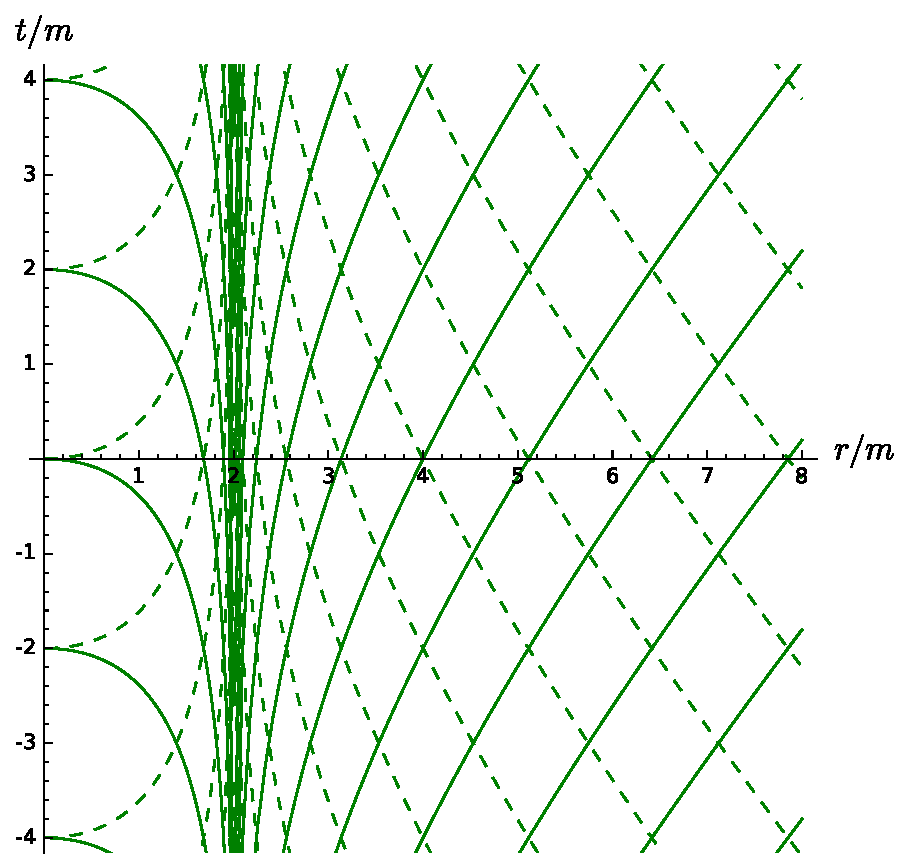
\includegraphics[width=0.6\textwidth]{sch_rad_null_geod.pdf}}
\caption[]{\label{f:sch:rad_null_geod} \footnotesize
Radial null geodesics of Schwarzschild spacetime, plotted in terms
of Schwarzschild-Droste coordinates $(t,r)$: the solid (resp. dashed) lines
correspond to outgoing (resp. ingoing) geodesics, as given by Eq.~(\ref{e:sch:outgoing_null_geod})
(resp. Eq.~(\ref{e:sch:ingoing_null_geod}).}
\end{figure}

\begin{itemize}
\item the \defin{outgoing radial null geodesics}\index{outgoing!null geodesic}, whose
equation is
\be \label{e:sch:outgoing_null_geod}
    t = r + 2 m \ln \left| \frac{r}{2m} - 1 \right| + u ,
\ee
where $u$ is a constant;
\item  the \defin{ingoing radial null geodesics}\index{ingoing!null geodesic}, whose
equation is
\be \label{e:sch:ingoing_null_geod}
    t = - r - 2 m \ln \left| \frac{r}{2m} - 1 \right| + v ,
\ee
where $v$ is a constant.
\end{itemize}



%%%%%%%%%%%%%%%%%%%%%%%%%%%%%%%%%%%%%%%%%%%%%%%%%%%%%%%%%%%%%%%%%%%%%%%%%%%%%%%

\section{Maximal extension}

\begin{figure}
\centerline{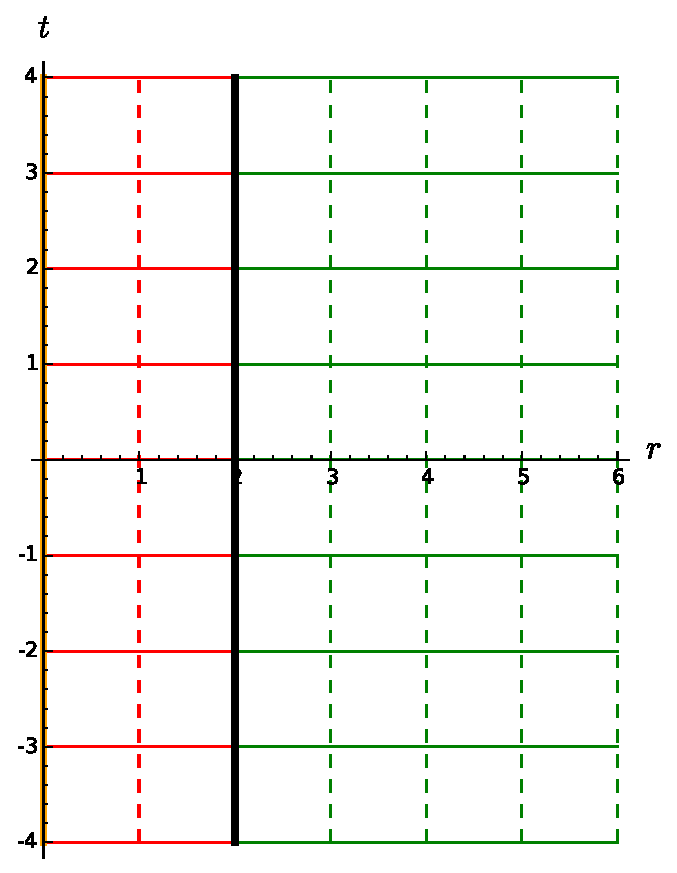
\includegraphics[height=0.37\textheight]{sch_coord_schwarz.pdf}\qquad
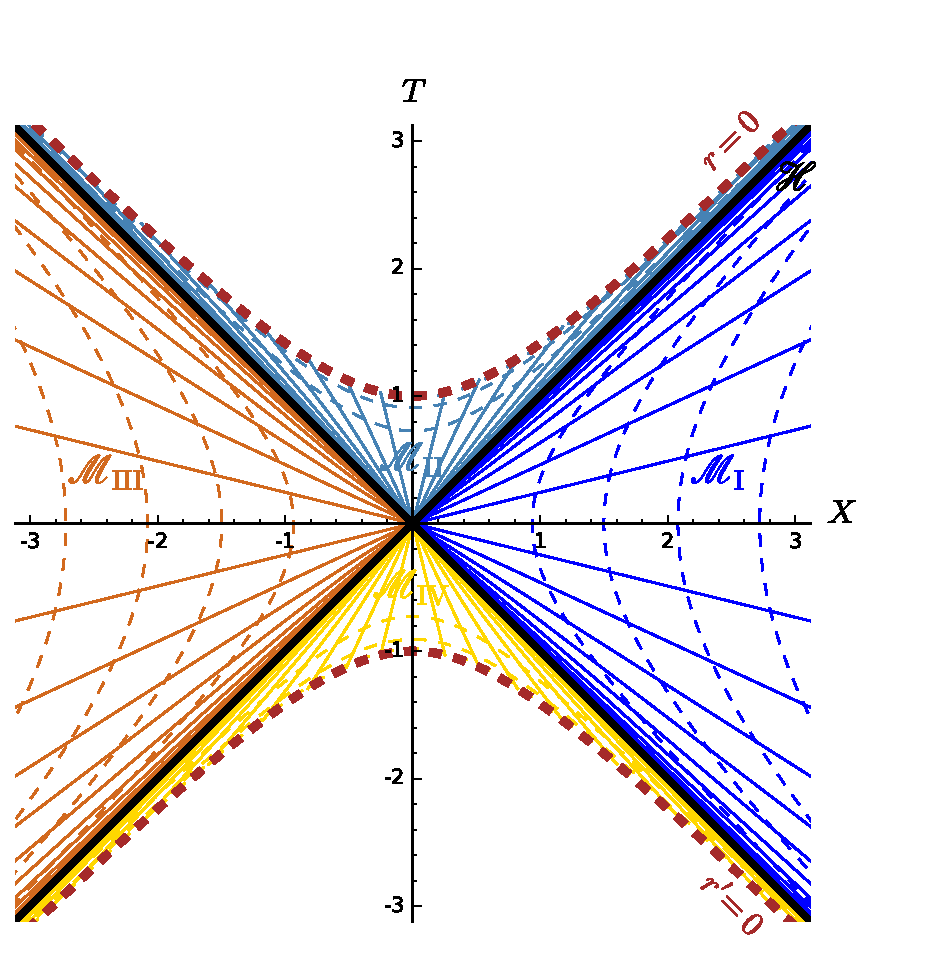
\includegraphics[height=0.37\textheight]{sch_kruskal_diag.pdf}}
\caption[]{\label{f:sch:kruskal_diag} \footnotesize
Schwarzschild spacetime depicted in Schwarzschild-Droste coordinates $(t,r)$
(left) and in Kruskal-Szekeres coordinates $(T,X)$ (right). In both figures,
green (resp. red) solid curves denote the hypersurfaces $t=\mathrm{const}$
in Region~I (resp. II), while green (resp. red) dashed curves
denote the hypersurfaces $r=\mathrm{const}$ in Region~I (resp. II).
The future and past event horizons are marked by thick black lines, while the
singularity at $r=0$ is depicted in orange. Regions III and IV are depicted
in grey and pink respectively. Note that the left figure covers only Regions I and II.}
\end{figure}

\begin{figure}
\centerline{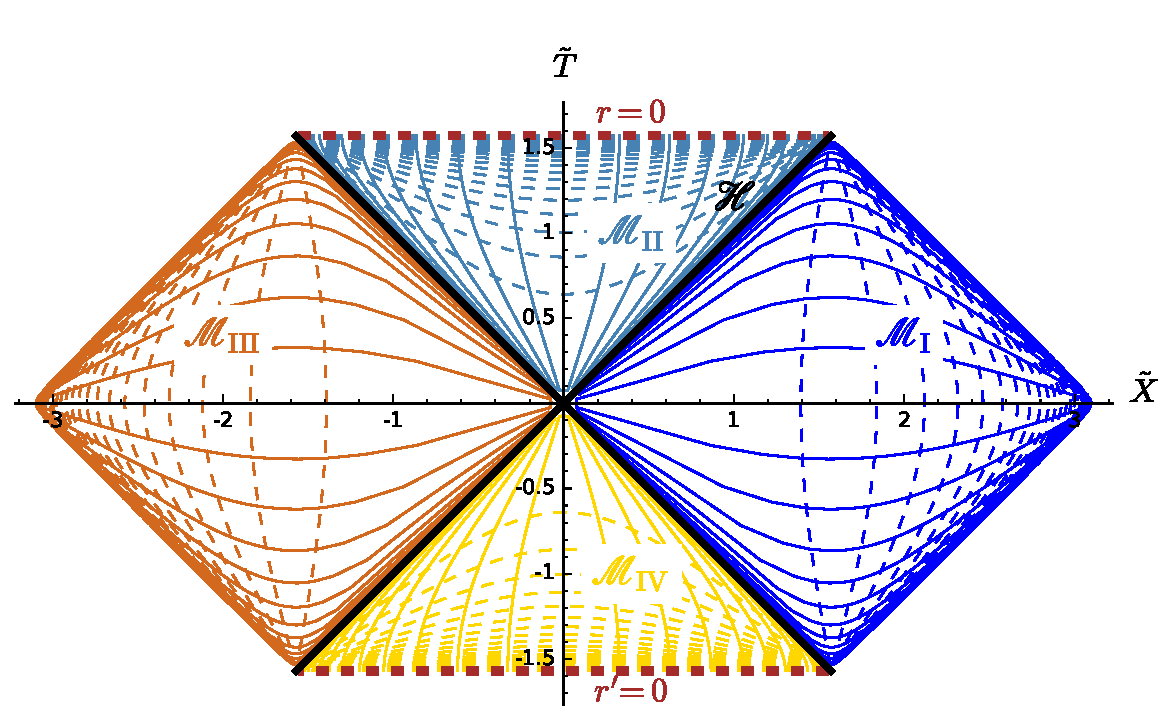
\includegraphics[width=0.9\textwidth]{sch_carter-penrose.pdf}}
\caption[]{\label{f:sch:sch_carter-penrose} \footnotesize
Schwarzschild spacetime depicted in Carter-Penrose coordinates $(\tilde{T},\tilde{X})$; the color code
is the same as in Fig.~\ref{f:sch:kruskal_diag}.
As Fig.~\ref{f:sch:kruskal_diag}, this figure has been produced with
SageManifolds (cf. Appendix~\ref{s:sam}).}
\end{figure}

  % Schwarzschild black hole

\chapter{Geodesics in Schwarzschild spacetime}

\chapter{Maximal extension of Schwarzschild spacetime}
\label{s:max}

\minitoc

\section{Introduction}


%%%%%%%%%%%%%%%%%%%%%%%%%%%%%%%%%%%%%%%%%%%%%%%%%%%%%%%%%%%%%%%%%%%%%%%%%%%%%%%


\section{Kruskal-Szekeres coordinates}

\subsection{Definition} \label{s:sch:KS_coord}

On the open set $\M_{\rm I}$, let us consider the ``double-null''
coordinate system $\hat{\hat{x}}^\alpha = (u,v,\th,\ph)$. It is related to
Schwarzschild-Droste coordinates $(t,r,\th,\ph)$ by
Eqs.~(\ref{e:sch:outgoing_null_geod})-(\ref{e:sch:ingoing_null_geod}):
\be \label{e:sch:u_v_r_t}
    \left\{\begin{array}{l}
    u = t - r - 2 m \ln \left| \frac{r}{2m} - 1 \right| \\[1ex]
    v = t + r + 2 m \ln \left| \frac{r}{2m} - 1 \right|
    \end{array}\right.
    \iff
        \left\{\begin{array}{l}
    t = \frac{1}{2} (u+v)\\[1ex]
    r + 2 m \ln \left| \frac{r}{2m} - 1 \right| = \frac{1}{2} (v-u).
    \end{array}\right.
\ee
Despite one cannot express explicitely $r$ in terms of $(u,v)$,
the function $r\mapsto r + 2 m \ln \left| \frac{r}{2m} - 1 \right|$ is
invertible on $(2m,+\infty)$ (cf. Fig.~\ref{f:sch:tortoise}), so that (\ref{e:sch:u_v_r_t}) does define a coordinate system on $\M_{\rm I}$.
The range of $(u,v)$ is $\R^2$.

The above relations imply
\[
 \D u = \D t - \frac{\D r}{1 - \frac{2m}{r}}  \qquad\mbox{and}\qquad
\D v = \D t + \frac{\D r}{1 - \frac{2m}{r}} .
\]
Hence
\[
    \D u \, \D v = \D t^2 - \frac{\D r^2}{\left(1 - \frac{2m}{r} \right) ^2} .
\]
The line element (\ref{e:sch:Schwarz_metric_SD}) becomes then
\be \label{e:sch:Schwarz_metric_uv}
    \encadre{
        \hat{\hat{g}}_{\mu\nu}\, \D \hat{\hat{x}}^\mu \,
        \D \hat{\hat{x}}^\nu =
            -\left( 1 - \frac{2 m}{r} \right)\, \D u \, \D v
       +  r^2 \left( \D\th^2 + \sin^2\th\, \D\ph^2 \right) }.
\ee
In this formula, $r$ is to be considered as a function of $(u,v)$, given
by (\ref{e:sch:u_v_r_t}).

\begin{figure}
\centerline{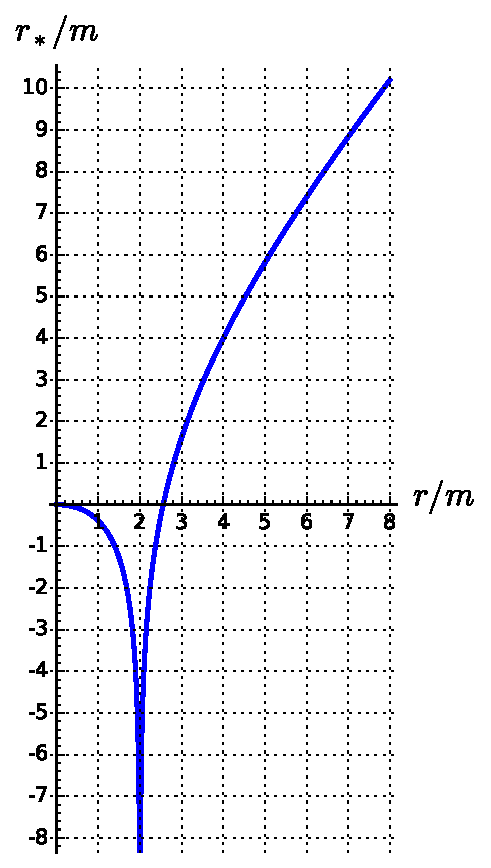
\includegraphics[height=0.4\textheight]{sch_tortoise.pdf}}
\caption[]{\label{f:sch:tortoise} \footnotesize
Function $r_*(r) = r + 2 m \ln \left| \frac{r}{2m} - 1 \right|$
(the tortoise coordinate, cf. Eq.~(\ref{e:sch:def_tortoise})).
It relates $r$ to $(u,v)$ via $r_*(r) = (u-v)/2$ [Eq.~(\ref{e:sch:u_v_r_t})].}
\end{figure}

The metric components (\ref{e:sch:Schwarz_metric_uv}) are regular on $\M_{\rm I}$.
Having a look at Fig.~\ref{f:sch:tortoise}, we realize that we cannot extend
this coordinate system to include the Schwarzschild horizon $\Hor$, since
$r\rightarrow 2m$ is equivalent to $v-u\rightarrow -\infty$: if $u$ (resp. $v$)
were taking a finite value on $\Hor$, we would have $v\rightarrow -\infty$
(resp. $u\rightarrow +\infty$). This impossibility of extending to $\Hor$
is also reflected by the fact that
\[
    \det \left( \hat{\hat{g}}_{\alpha\beta} \right) =
        - \frac{1}{4} \left( 1 - \frac{2 m}{r} \right) ^2 r^4 \sin^2\th
\]
vanishes for $r\rightarrow 2m$, which would make $\w{g}$ a degenerate bilinear
form at $r=2m$, while it is not of course.

Instead of $(u,v)$, let us use on $\M_{\rm I}$
the coordinates $(U,V)$ defined by
\be \label{e:sch:def_U_V}
    \left\{\begin{array}{l}
    U := - \mathrm{e}^{-u/4m} \\
    V := \mathrm{e}^{v/4m} .
    \end{array}\right.
\ee
Since the range of $(u,v)$ is $\R^2$, the range of $U$ is $(-\infty,0)$
and that of $V$ is $(0,+\infty)$.
We have
\[
    \D U = \frac{1}{4m} \,  \mathrm{e}^{-u/4m}  \, \D u\qquad\mbox{and}\qquad
    \D V = \frac{1}{4m} \,  \mathrm{e}^{v/4m} \, \D v ,
\]
hence
\[
    \D u \, \D v = 16 m^2 \mathrm{e}^{(u-v)/4m} \, \D U \, \D V .
\]
Now, on $\M_{\rm I}$, $r>2m$ and (\ref{e:sch:u_v_r_t}) yields
\be \label{e:sch:r_u_v_exp}
    r + 2 m \ln \left( \frac{r}{2m} - 1 \right) = \frac{1}{2} (v-u)
    \quad
    \Longrightarrow
    \quad
     \mathrm{e}^{r/2m} \left( \frac{r}{2m} - 1 \right)  =
    \mathrm{e}^{(v-u)/4m}  ,
\ee
so that
\[
     \D u \, \D v = 16 m^2 \, \mathrm{e}^{-r/2m}
        \left( \frac{r}{2m} - 1 \right) ^{-1} \D U \, \D V
        = \frac{32 m^3}{r} \, \mathrm{e}^{-r/2m}
        \left( 1 - \frac{2m}{r} \right) ^{-1} \D U \, \D V .
\]
Substituting this expression in (\ref{e:sch:Schwarz_metric_uv}) yields
the expression of the metric components with respect to
coordinates ${\hat X}^\alpha := (U,V,\th,\ph)$:
\be \label{e:sch:metric_UV}
    \encadre{
    g_{\mu\nu} \, \D {\hat X}^\mu \, \D {\hat X}^\nu =
    - \frac{32 m^3}{r} \, \mathrm{e}^{-r/2m} \,  \D U \, \D V
     +  r^2 \left( \D\th^2 + \sin^2\th\, \D\ph^2 \right) }.
\ee
In this formula, $r$ has to be considered as a function of $(U,V)$, whose
implicit expression is found by combining
(\ref{e:sch:def_U_V}) and (\ref{e:sch:r_u_v_exp}):
\be \label{e:max:r_UV_M_I}
    \encadre{ \mathrm{e}^{r/2m} \left( \frac{r}{2m} - 1 \right) = - U V } .
\ee
\begin{remark}
This relation takes a very simple form in terms of the tortoise coordinate
(cf. Eq.~(\ref{e:sch:def_tortoise})):
\be
    \mathrm{e}^{r_*/2m} = - U V  .
\ee
\end{remark}

We notice that the factor $(1-2m/r)$ has disappeared in the line
element (\ref{e:sch:metric_UV}), which becomes perfectly regular as
$r\rightarrow 2m$.

We read on (\ref{e:sch:metric_UV}) that $g_{UU} = 0$ and $g_{VV} = 0$.
Hence $(U,V)$ is a double-null coordinate system, as much as $(u,v)$.
To cope with a timelike-spacelike coordinate system instead, let
us introduce on $\M_{\rm I}$ the pair $(T,X)$ such that $U$ is $T$
retarded by $X$ and $V$ is $T$ advanced by $X$:
\be \label{e:sch:def_T_X}
    \left\{\begin{array}{l}
    U = T - X\\
    V = T + X
    \end{array}\right.
    \qquad \iff\qquad
    \left\{\begin{array}{l}
    T = \frac{1}{2} (U+V) \\[1ex]
    X = \frac{1}{2} (V-U)
    \end{array}\right.
\ee
Since the range of $U$ on $\M_{\rm I}$ is $(-\infty,0)$ and that of $V$ is
$(0,+\infty)$, the range of $(T,X)$ is ruled by $T<X$, $T>-X$ and $X>0$.
In other words, the coordinates $(T,X)$ span the following quarter of
$\mathbb{R}^2$ (cf. Fig.~\ref{f:sch:SD_I_KS}):
\be \label{e:sch:X_T_range_I}
    \M_{\rm I}: \quad X > 0 \quad\mbox{and}\quad -X < T < X .
\ee
The coordinates $X^\alpha := (T,X,\th,\ph)$ are called
the \defin{Kruskal-Szekeres coordinates}\index{Kruskal-Szekeres!coordinates}.

\begin{figure}
\centerline{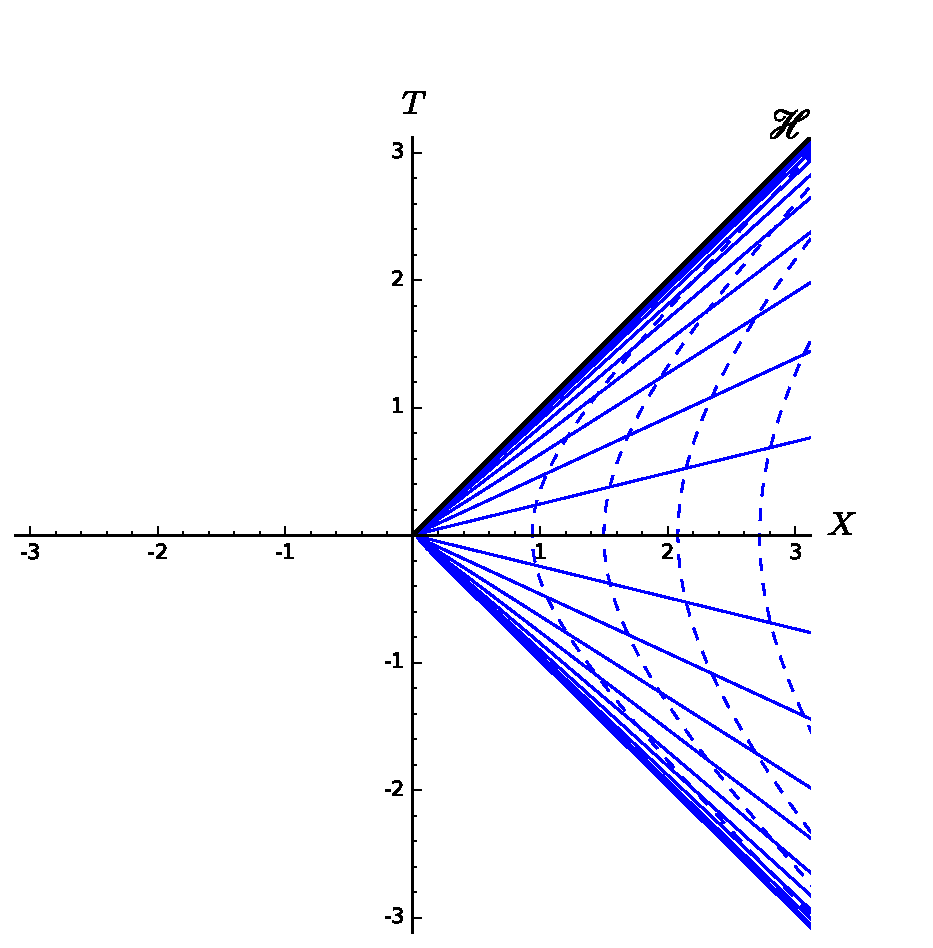
\includegraphics[width=0.6\textwidth]{sch_SD_I_KS.pdf}}
\caption[]{\label{f:sch:SD_I_KS} \footnotesize
Submanifold $\M_{\rm I}$ in the Kruskal-Szekeres coordinates $(T,X)$:
$\M_{\rm I}$ is covered by the Schwarzschild-Droste grid (in blue): the solid
lines have $t=\mathrm{const}$ (spaced apart by $\delta t = m$), while the
dashed curves have $r=\mathrm{const}$ (spaced apart by $\delta r = m/2$).}
\end{figure}


\begin{figure}
\centerline{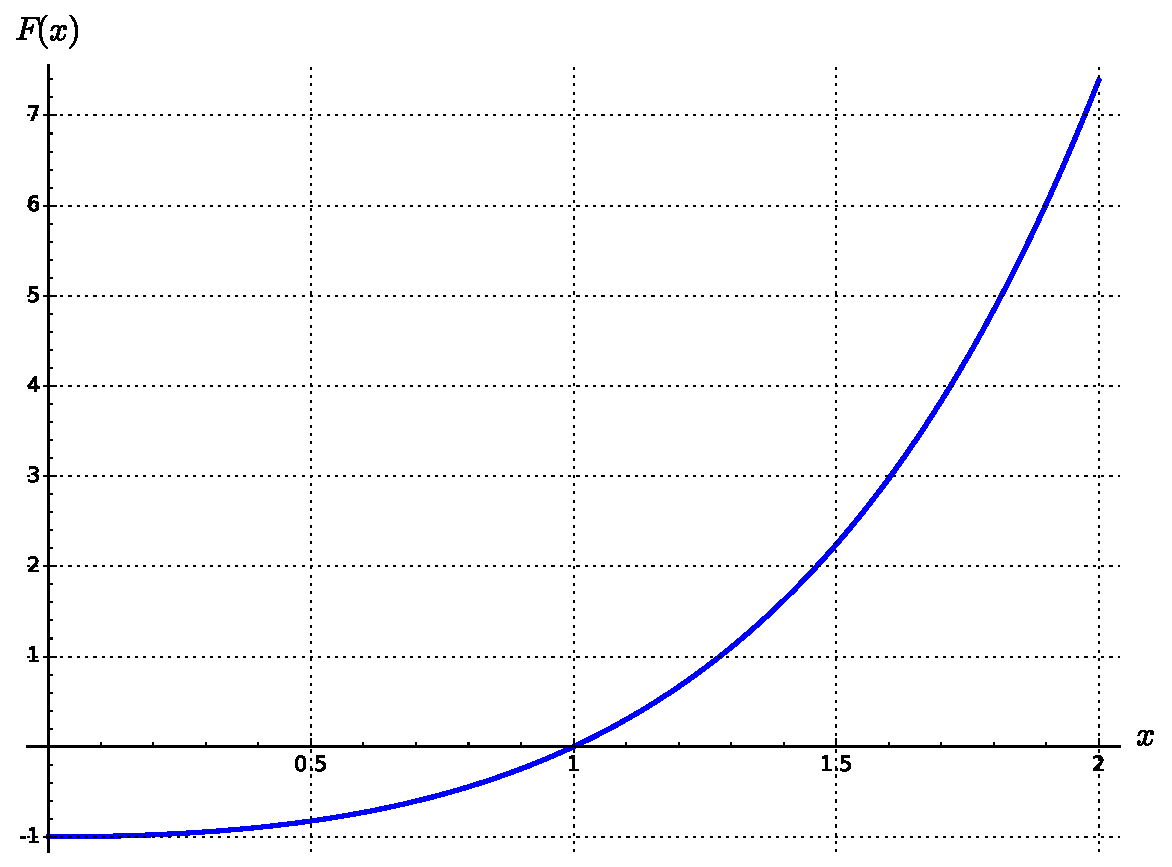
\includegraphics[height=0.37\textheight]{max_X2mT2.pdf}}
\caption[]{\label{f:max:X2mT2} \footnotesize
Function $F:\; x\mapsto \mathrm{e}^{x}(x-1)$, yielding
$X^2-T^2 = F(r/2m)$, cf. Eq.~(\ref{e:sch:X2mT2}).}
\end{figure}

We have $\D U \, \D V = (\D T - \D X) (\D T + \D X)  = \D T^2 - \D X^2$,
so that the metric components with respect to the Kruskal-Szekeres coordinates
are easily deduced from the line element (\ref{e:sch:metric_UV}):
\be \label{e:sch:metric_KS}
    \encadre{
    g_{\mu\nu} \, \D X^\mu \, \D X^\nu =
    \frac{32 m^3}{r} \, \mathrm{e}^{-r/2m}
    \left( - \D T^2 + \D X^2 \right)
     +  r^2 \left( \D\th^2 + \sin^2\th\, \D\ph^2 \right) }.
\ee
Here $r$ is to be considered as a function of $(T,X)$, which is implicitely defined
by
\be \label{e:sch:X2mT2}
   \encadre{ \mathrm{e}^{r/2m} \left( \frac{r}{2m} - 1 \right) = X^2 - T^2 } .
\ee
This relation is a direct consequence of (\ref{e:max:r_UV_M_I}) and (\ref{e:sch:def_T_X}).
We may rewrite it as
\be
    F\left( \frac{r}{2m} \right) = X^2 - T^2,
\ee
where $F$ is the function defined by
\be \label{e:sch:def_F}
    \begin{array}{cccc}
    F: & (0,+\infty) & \longrightarrow & (-1,+\infty) \\
        & x & \longmapsto & \mathrm{e}^{x}(x-1) .
    \end{array}
\ee
The graph of $F$  is shown in Fig.~\ref{f:max:X2mT2}. We see clearly that $F$ is a bijective map.
In particular, $F$ induces a bijection between $(1,+\infty)$ (the range of $r/2m$ on $\M_{\rm I}$)
and $(0,+\infty)$ (the range of $X^2-T^2$ on $\M_{\rm I}$, according to (\ref{e:sch:X_T_range_I})). The inverse of $F$ can be expressed in terms of
the \defin{Lambert function}\index{Lambert function} $W_0$, which is defined as
the inverse of $x\mapsto x \mathrm{e}^x$:
\be \label{e:sch:def_W0}
    \begin{array}{cccl}
    W_0: & (-1/\mathrm{e},+\infty) & \longrightarrow & (-1,+\infty) \\
        & x & \longmapsto & y \mbox{\ such that\ } y \mathrm{e}^{y} = x .
    \end{array}
\ee
Noticing that
\[
    F(x) = \mathrm{e}^x(x-1) = \mathrm{e}\times (x-1) \mathrm{e}^{x-1}
\]
we may write
\be
    F^{-1} = \tilde{W}_0 ,
\ee
where $\tilde{W}_0$ is the rescaled Lambert function defined by
\be \label{e:max:def_tilde_W0}
    \encadre{ \tilde{W}_0(x) := W_0\left(\frac{x}{\mathrm{e}}\right) + 1 }.
\ee
Note that $\tilde{W}_0$ is a bijection $(-1,+\infty) \to (0, +\infty)$, which
obeys
\be \label{e:max:exp_tW0}
    \mathrm{e}^{\tilde{W}_0(x)} \left( \tilde{W}_0(x) - 1 \right) = x .
\ee
Its graph is shown in Fig.~\ref{f:max:lambert_rescaled}.

\begin{figure}
\centerline{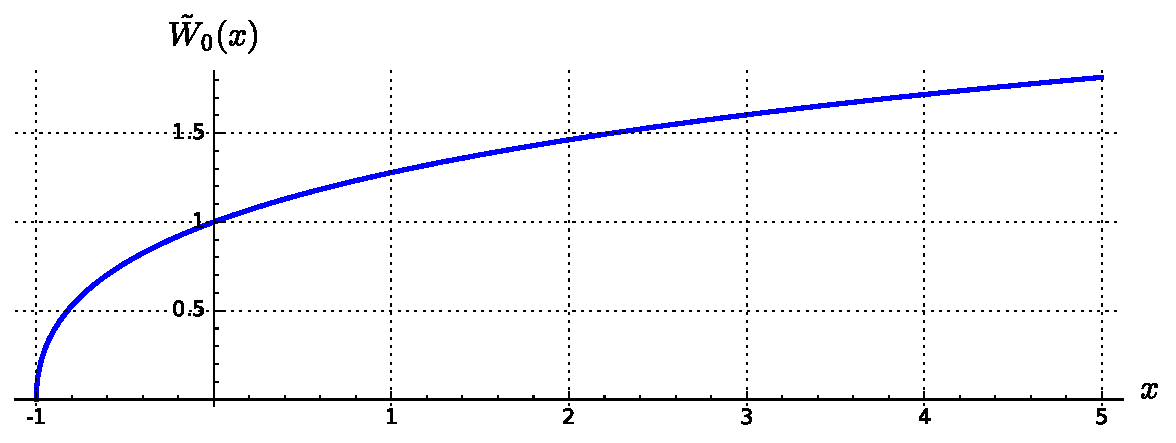
\includegraphics[width=0.8\textwidth]{max_lambert_rescaled.pdf}}
\caption[]{\label{f:max:lambert_rescaled} \footnotesize
Rescaled lambert function $\tilde{W}_0$, defined by (\ref{e:max:def_tilde_W0})
and obeying
$\mathrm{e}^{\tilde{W}_0(x)}(\tilde{W}_0(x)-1) = x$.}
\end{figure}

Using $F^{-1} = \tilde{W}_0$, we may invert the relation (\ref{e:sch:X2mT2})
to $r = 2m \tilde{W}_0(X^2-T^2)$. Noticing that
$2m/r \, \mathrm{e}^{-r/2m} = (X^2-T^2 + \mathrm{e}^{r/2m})^{-1}$
[cf. Eq.~(\ref{e:sch:X2mT2})], we may eliminate $r$ from the expression
(\ref{e:sch:metric_KS})
of the metric components in Kruskal-Szekeres coordinates:
\be \label{e:sch:metric_KS_TX_partial}
   \encadre{
    \begin{array}{lcll}
    g_{\mu\nu} \, \D X^\mu \, \D X^\nu & = & 4m^2 \bigg\{ & \displaystyle
    \frac{4}{X^2-T^2 + \mathrm{e}^{\tilde{W}_0(X^2-T^2)} }
    \left( - \D T^2 + \D X^2 \right) \\[2ex]
    & & & \displaystyle + \,   \tilde{W}_0(X^2-T^2)^2 \left( \D\th^2 + \sin^2\th\, \D\ph^2 \right)
    \bigg\}.
    \end{array} }
\ee


The relation between the Kruskal-Szekeres coordinates and the
Schwarzschild-Droste ones is obtained by combining (\ref{e:sch:def_T_X}),
(\ref{e:sch:def_U_V}) and (\ref{e:sch:u_v_r_t}):
\bea
    T &=& \frac{1}{2}(U+V) = \frac{1}{2} \left( \mathrm{e}^{v/4m}
        - \mathrm{e}^{-u/4m)} \right) =
        \frac{1}{2} \left( \mathrm{e}^{(t+r_*)/4m}
        - \mathrm{e}^{(r_*-t)/4m} \right) \nonumber \\
     & = & \mathrm{e}^{r_*/4m} \sinh\left( \frac{t}{4m} \right) ,\nonumber
\eea
where $r_*$ is related to $r$ by (\ref{e:sch:def_tortoise}).
Similarly
\[
     X = \mathrm{e}^{r_*/4m} \cosh\left( \frac{t}{4m} \right) .
\]
In particular, we have
\be \label{e:max:TsX_tanh_t}
    \frac{T}{X} = \tanh\left( \frac{t}{4m} \right) .
\ee
From Eq.~(\ref{e:sch:def_tortoise}), we have
\[
    \mathrm{e}^{r_*/4m} = \mathrm{e}^{r/4m} \sqrt{ \frac{r}{2m} - 1 } .
\]
We may summarize the above relations as follows:
\be \label{e:sch:KS_SD_I}
    \M_{\rm I}: \quad \encadre{ \left\{\begin{array}{l}
    T = \mathrm{e}^{r/4m} \sqrt{ \frac{r}{2m} - 1 } \sinh\left( \frac{t}{4m} \right)
\\[2ex]
    X = \mathrm{e}^{r/4m} \sqrt{ \frac{r}{2m} - 1 } \cosh\left( \frac{t}{4m} \right)
        \end{array}\right. }
    \iff
    \encadre{ \left\{\begin{array}{l}
    t = 2 m \,  \ln \left( \frac{X+T}{X-T} \right) \\[2ex]
    r = 2 m \tilde{W}_0(X^2 - T^2) .
        \end{array}\right. }
\ee
Note that we have used the identity $\mathrm{artanh}\, x = 1/2 \ln\left[(1+x)/(1-x)\right]$.
The curves of constant $t$ and constant $r$ in the $(T,X)$ plane
are drawn in Fig.~\ref{f:sch:SD_I_KS}.
The fact that the curves of constant $t$ are straight lines from the
origin follow immediately
from Eq.~(\ref{e:max:TsX_tanh_t}).

\begin{remark}
Given the properties of the $\cosh$ and $\sinh$ functions, it is clear on these
expressions that the constraints (\ref{e:sch:X_T_range_I}) are satisfied.
\end{remark}
\begin{remark}
In line element (\ref{e:sch:metric_KS_TX_partial})
the metric components $g_{TT}$ and $g_{XX}$ depend on both $X$ and $T$; this
shows that neither $\wpar_T$ nor $\wpar_X$ coincide with a Killing vector.
In other words, the coordinates $(T,X)$ are not adapted to the spacetime
symmetries, contrary to the Schwarzschild-Droste coordinates or to the
Eddington-Finkelstein ones.
\end{remark}

\subsection{Extension to the IEF domain}

We notice that the metric components (\ref{e:sch:metric_KS}) are perfectly
regular at $r=2m$. Therefore the Kruskal-Szekeres coordinates can be extended
to cover the Schwarzschild horizon $\Hor$. Actually they can be extended to
all values of $r\in (0,2m]$, i.e. to the whole domain of the ingoing
Eddington-Finkelstein coordinates: the manifold $\M_{\rm IEF}$ introduced
in Sec.~\ref{s:sch:Schwarz_hor}:
$\M_{\rm IEF} = \M_{\rm I} \cup \Hor \cup \M_{\rm II}$. Let us show
this in detail. Back on $\M_{\rm I}$, we can express the IEF coordinate
$\ti$ in terms of $(T,X)$ by combining $\ti = v - r$ [Eq.~(\ref{e:sch:ti_v_r})],
$v = 4m\ln V$ [Eq.~(\ref{e:sch:def_U_V})] and $V = T+X$ [Eq.~(\ref{e:sch:def_T_X})]:
\be
    \ti = 4 m \ln (T+X) - r.
\ee
The above relation is a valid expression as long as $T+X>0$.
Besides, we already noticed
that the function $F$ defined by (\ref{e:sch:def_F}) is a bijection from the range of $r/2m$
on $\M_{\rm IEF}$, i.e. $(0,+\infty)$, to $(-1,+\infty)$, with the
$(0,+\infty)$ part of the latter interval representing the range of $X^2-T^2$
on $\M_{\rm I}$. We may use these properties to extend the Kruskal-Szekeres coordinates to all $\M_{\rm IEF}$ by requiring
\begin{subequations}\label{e:sch:ti_r_X_T}
\begin{align}
 & \ti = 4 m \ln (T+X) - r\\
 & \underbrace{\mathrm{e}^{r/2m} \left( \frac{r}{2m} - 1 \right)}_{F(r/2m)} = X^2-T^2 .
 \end{align}
\end{subequations}
The range of the coordinates $(T,X)$ on $\M_{\rm IEF}$ is then ruled by
\[
    \M_{\rm IEF}:\quad T+X > 0 \quad\mbox{and}\quad X^2 - T^2 > -1 ,
\]
which can be rewritten as
\be \label{e:sch:range_X_T_IEF}
    \M_{\rm IEF}: \quad -X < T < \sqrt{X^2+1}.
\ee
We deduce from (\ref{e:sch:ti_r_X_T}) that
\be \label{e:sch:KS_IEF_prov}
    \left\{\begin{array}{lcl}
    X+T & = & \mathrm{e}^{(\ti+r)/4m} \\
    X-T & = & \mathrm{e}^{(r -\ti)/4m} \left( \frac{r}{2m} - 1 \right) .
    \end{array}\right.
\ee
Hence the relation between the ingoing Eddington-Finkelstein coordinates and
the Kruskal-Szekeres ones on $\M_{\rm IEF}$:
\be \label{e:sch:KS_IEF}
    \encadre{ \left\{\begin{array}{l}
    T = \mathrm{e}^{r/4m} \left[ \cosh\left(\frac{\ti}{4m}\right)
        - \frac{r}{4m} \mathrm{e}^{-\ti/4m} \right] \\[2ex]
    X =  \mathrm{e}^{r/4m} \left[ \sinh\left(\frac{\ti}{4m}\right)
        + \frac{r}{4m} \mathrm{e}^{-\ti/4m}  \right]
    \end{array}\right. }
    \iff
    \encadre{\left\{\begin{array}{l}
     \ti =  2 m \left[ 2 \ln (T+X) - \tilde{W}_0(X^2 - T^2) \right] \\[1ex]
    r = 2 m \tilde{W}_0(X^2 - T^2)
    \end{array}\right. }
\ee
The various subsets of $\M_{\rm IEF}$ correspond then to the following
coordinate ranges (cf. Fig.~\ref{f:sch:IEF_KS}):
\begin{subequations}
\label{e:max:range_TX_M_I_II}
\begin{align}
 & \M_{\rm I}: \quad X > 0 \quad\mbox{and}\quad -X < T < X \\
 & \Hor: \quad X > 0 \quad\mbox{and}\quad  T = X \\
 & \M_{\rm II}: \quad |X| < T < \sqrt{X^2+1} .
\end{align}
\end{subequations}

\begin{figure}
\centerline{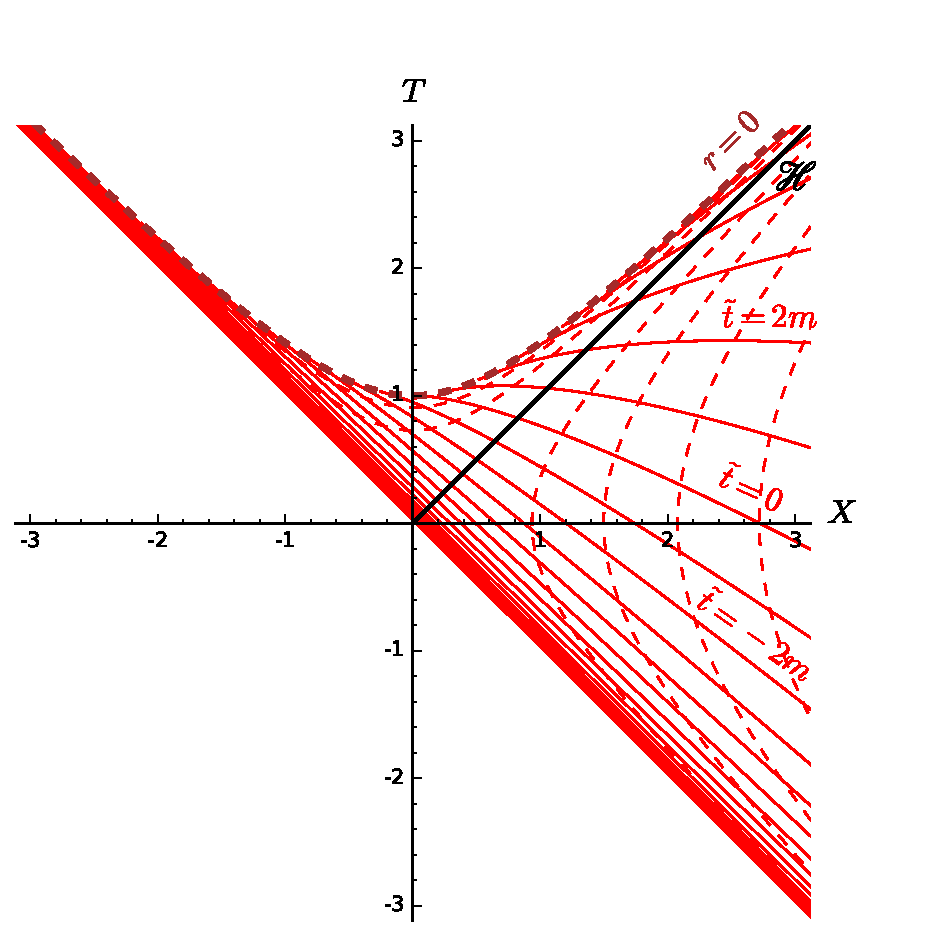
\includegraphics[width=0.6\textwidth]{sch_IEF_KS.pdf}}
\caption[]{\label{f:sch:IEF_KS} \footnotesize
Domain of ingoing Eddington-Finkelstein coordinates, $\M_{\rm IEF} = \M_{\rm I}\cup \Hor\cup \M_{\rm II}$, depicted in terms of the Kruskal-Szekeres coordinates $(T,X)$: the solid red
curves have $\ti=\mathrm{const}$ (spaced apart by $\delta\ti = m$), while the
dashed red curves have $r=\mathrm{const}$ (spaced apart by $\delta r = m/2$).}
\end{figure}


Since the relation between IEF coordinates and Kruskal-Szekeres ones is the
same in $\M_{\rm II}$ as in $\M_{\rm I}$ (being given by (\ref{e:sch:KS_IEF})
in both cases), we conclude that the expression (\ref{e:sch:metric_KS})
of the metric components with respect to
Kruskal-Szekeres coordinates is valid in all $\M_{\rm IEF}$.

Let us determine the relation between the Kruskal-Szekeres coordinates and
the Schwarz\-schild-Droste ones in $\M_{\rm II}$. Since $r<2m$ in $\M_{\rm II}$,
Eq.~(\ref{e:sch:ti_t_r}) gives
\[
    \M_{\rm II}: \quad  \mathrm{e}^{\ti/4m} = \mathrm{e}^{t/4m}  \sqrt{1 -  \frac{r}{2m} } ,
\]
so that (\ref{e:sch:KS_IEF_prov}) can be rewritten as
\[
     \M_{\rm II}: \quad
\left\{\begin{array}{lcl}
    X+T & = & \displaystyle \mathrm{e}^{(t+r)/4m} \sqrt{1 -  \frac{r}{2m} }  \\[2ex]
    X-T & = & \displaystyle  - \mathrm{e}^{(r -t)/4m}  \sqrt{1 -  \frac{r}{2m} }.
    \end{array}\right.
\]
We obtain then
\be \label{e:sch:KS_SD_II}
    \M_{\rm II}: \quad \encadre{ \left\{\begin{array}{l}
    T = \mathrm{e}^{r/4m} \sqrt{ 1 - \frac{r}{2m} } \cosh\left( \frac{t}{4m} \right)
\\[2ex]
    X = \mathrm{e}^{r/4m} \sqrt{ 1 - \frac{r}{2m} } \sinh\left( \frac{t}{4m} \right)
        \end{array}\right. }
    \iff
    \encadre{ \left\{\begin{array}{l}
    t = 2 m \,  \ln \left( \frac{T+X}{T-X} \right) \\[2ex]
    r = 2 m \tilde{W}_0(X^2 - T^2) .
        \end{array}\right. }
\ee
This is to be compared with (\ref{e:sch:KS_SD_I}).
The curves of constant $t$ and constant $r$ in the $(T,X)$ plane
are drawn in Fig.~\ref{f:sch:SD_KS}, which extends Fig.~\ref{f:sch:SD_I_KS}
to $\M_{\rm II}$.

\begin{figure}
\centerline{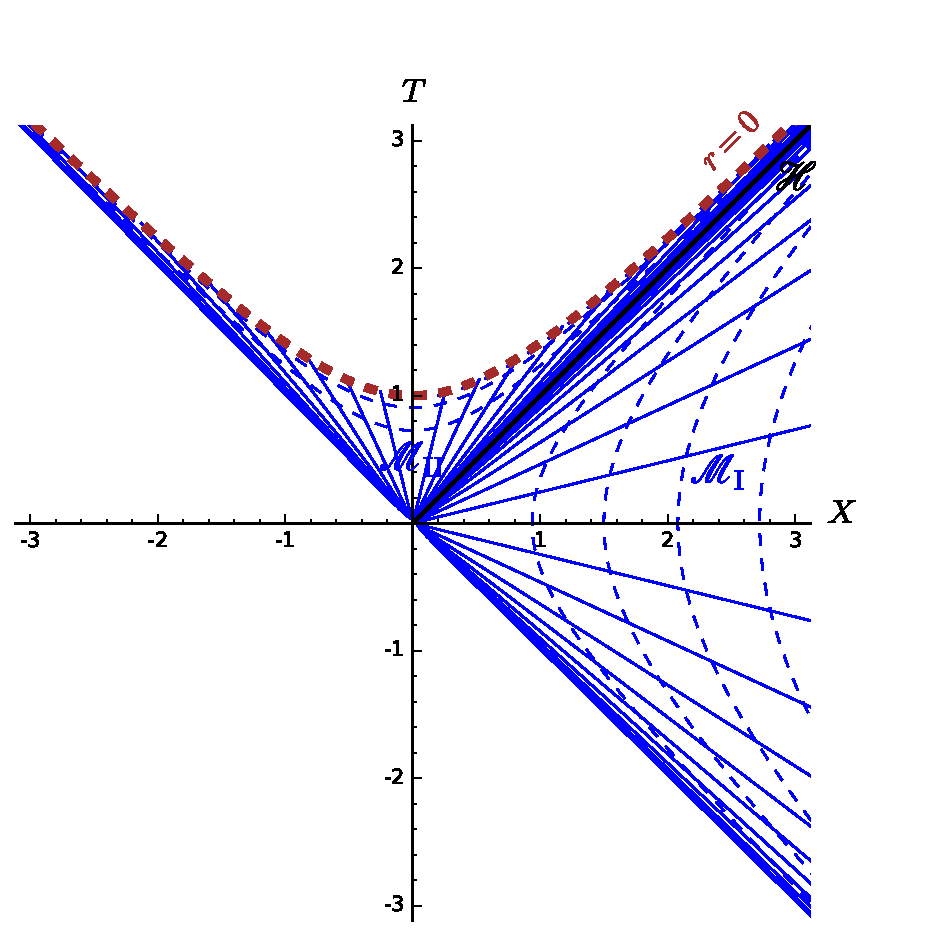
\includegraphics[width=0.6\textwidth]{sch_SD_KS.pdf}}
\caption[]{\label{f:sch:SD_KS} \footnotesize
Schwarzschild-Droste coordinates in $\M_{\rm SD} = \M_{\rm I}\cup \M_{\rm II}$
depicted in terms of the Kruskal-Szekeres coordinates $(T,X)$: the solid blue
curves have $t=\mathrm{const}$ (spaced apart by $\delta t = m$), while the
dashed blue curves have $r=\mathrm{const}$ (spaced apart by $\delta r = m/2$).}
\end{figure}


As discussed in Sec.~\ref{s:sch:singularities}, one approaches a
curvature singularity as $r\rightarrow 0$. According to (\ref{e:sch:KS_IEF})
or (\ref{e:sch:KS_SD_II}),
this corresponds to $X^2-T^2 \rightarrow -1$ (see also Fig.~\ref{f:max:X2mT2}), with
$T > 0$. Hence, in the $(T,X)$ plane, the curvature singularity is located
at $T = \sqrt{X^2 + 1}$, i.e. at the upper branch of the hyperbola
$T^2 - X^2 = 1$.

\subsection{Radial null geodesics in Kruskal-Szekeres coordinates}
\label{s:sch:rad_null_geod_KS}

By construction, the Kruskal-Szekeres coordinates $(T,X,\th,\ph)$ are
adapted to the radial null geodesics. This is clear on the expression
(\ref{e:sch:metric_KS}) of the metric tensor, where the $(T,X)$ part is
conformal to the flat metric $- \D T^2 + \D X^2$. Consequently the radial
null geodesics are straight lines of slope $\pm 45^\circ$ in the $(T,X)$ plane
(cf. Fig.~\ref{f:sch:rad_null_geod_KS}):
\begin{itemize}
\item the ingoing radial null geodesics obey
\be \label{e:sch:ingoing_null_geod_KS}
    T = - X + V ,
\ee
where $V$ is a positive constant (the constraint $V>0$ following from (\ref{e:sch:range_X_T_IEF})), so that each geodesic of this family can be labelled
by $(V,\th,\ph)$;
\item the outgoing radial null geodesics obey
\be \label{e:sch:outgoing_null_geod_KS}
    T = X + U ,
\ee
where $U$ is an arbitrary real constant, so that each geodesic of this family can be labelled
by $(U,\th,\ph)$.
\end{itemize}
\begin{figure}
\centerline{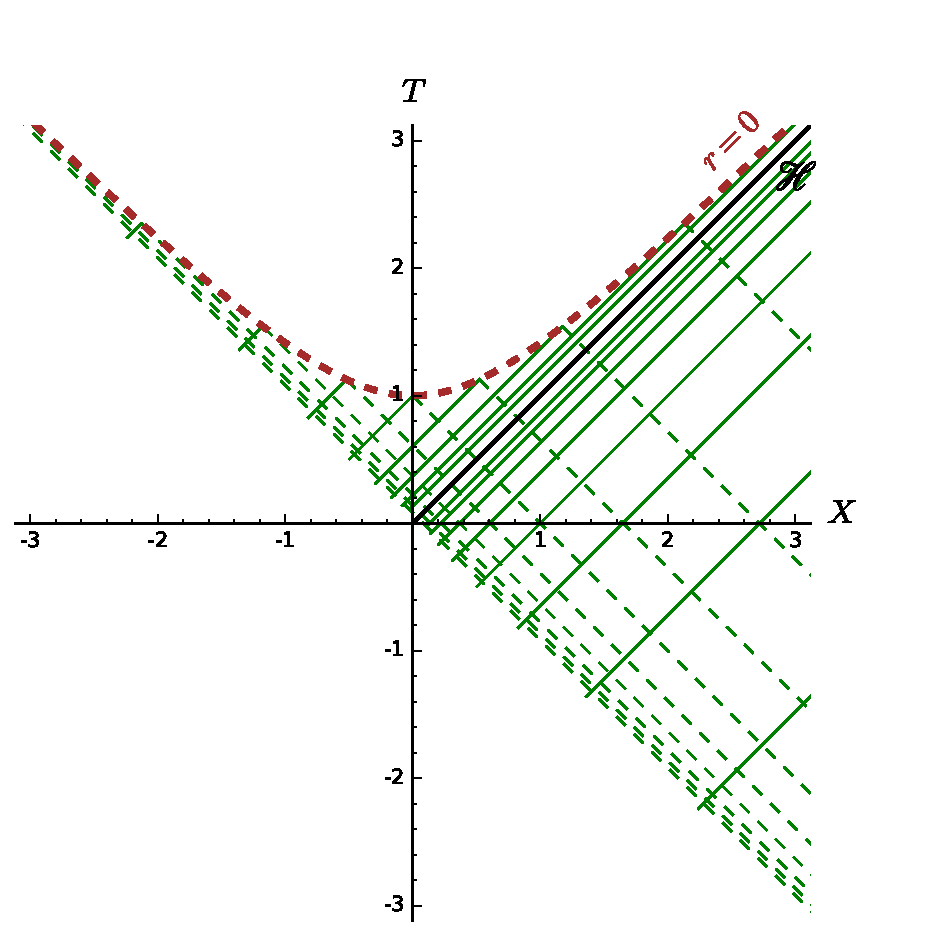
\includegraphics[width=0.6\textwidth]{sch_rad_null_geod_KS.pdf}}
\caption[]{\label{f:sch:rad_null_geod_KS} \footnotesize
Radial null geodesics in $\M_{\rm IEF} = \M_{\rm I}\cup\Hor\cup\M_{\rm II}$
depicted in terms of the Kruskal-Szekeres coordinates $(T,X)$: the solid
lines correspond to the outgoing family, with $u$ spanning $[-6m, 8m]$
(with steps $\delta u = 2m$), from the left to the right in $\M_{\rm II}$
and from the right to the left in $\M_{\rm I}$; the dashed lines
correspond to the ingoing family, with $v$ spanning $[-8m, 6m]$ (with steps $\delta v = 2m$)
from the left to the right.}
\end{figure}
In particular, the Schwarzschild horizon $\Hor$ is generated by the
outgoing radial null geodesics having $U=0$:
Eqs.~(\ref{e:sch:outgoing_null_geod_KS}) and (\ref{e:sch:X2mT2})
clearly imply $r=2m$ for $U=0$, i.e. $X=T$.
 The outgoing radial null geodesics not lying on $\Hor$ have an equation
in terms of the IEF coordinates given by
Eq.~(\ref{e:sch:outgoing_null_geod_EF}):
$\ti = r + 4 m \ln \left|r/2m- 1 \right| + u$,
where the constant $u$ is related to $U$ by
\begin{subequations}
\begin{align}
 & U = - \mathrm{e}^{-u/4m} \quad \mbox{on}\ \M_{\rm I} \\
 & U = 0 \quad \mbox{on}\ \Hor \\
 & U =  \mathrm{e}^{-u/4m} \quad \mbox{on}\ \M_{\rm II} .
\end{align}
\end{subequations}
These relations are easily established by combining
(\ref{e:sch:outgoing_null_geod_EF}) and (\ref{e:sch:KS_IEF}).


\begin{remark}
The relation $U = - \mathrm{e}^{-u/4m}$ introduced in Sec.~\ref{s:sch:KS_coord}
by Eq.~(\ref{e:sch:def_U_V}) is thus valid only in $\M_{\rm I}$. On the
contrary the relation $V = \mathrm{e}^{v/4m}$ is valid in all $\M_{\rm IEF}$.
\end{remark}

\section{Maximal extension} \label{s:sch:max_extens}

\subsection{Construction} \label{s:sch:max_extens_constr}

The spacetime $(\M_{\rm IEF}, \w{g})$ is not geodesically complete.
Indeed, let us consider the radial null geodesics discussed above.
We have seen in Sec.~\ref{s:sch:rad_null_geod} that $r$ is an affine parameter
along them, except for those that are null generators of $\Hor$
(the outgoing ones with $U=0$).
Now, for the ingoing radial null geodesics, $r$ is decreasing towards the
future and all of them terminate at $r=0$ (the left end-point of the dashed
lines in Fig.~\ref{f:sch:rad_null_geod_KS}).
They are thus incomplete geodesics. However, they cannot be extended to
negative values of the affine parameter $r$ by extending the spacetime
since $r=0$ marks a spacetime singularity (cf. Sec.~\ref{s:sch:singularities}).

On the other hand the outgoing radial null geodesics are limited by
the constraint $T+X > 0$, which corresponds to $r>2m$ in $\M_{\rm I}$, with $r$ increasing towards
the future, and to
$r<2m$ in $\M_{\rm II}$, with $r$ decreasing towards the future.
Thus all outgoing radial null geodesics terminate towards the past at the finite
value $2m$ of the affine parameter $r$
(the left end point of the solid lines in Fig.~\ref{f:sch:rad_null_geod_KS}) and are therefore incomplete geodesics.
However, contrary to ingoing radial null geodesics, they can be extended
since $r=2m$ does not mark any spacetime singularity.
More precisely, the limit at which outgoing radial null geodesics
terminate is $T=-X$, which by virtue of (\ref{e:sch:X2mT2}) yields $r=2m$.
This does not correspond to the Schwarzschild horizon $\Hor$, since for
the latter $T=X$, but rather to $\ti\rightarrow-\infty$,
as it is clear when comparing Fig.~\ref{f:sch:rad_null_geod_KS}
with Fig.~\ref{f:sch:IEF_KS}.

Another hint regarding the extendability of $(\M_{\rm IEF}, \w{g})$
is the fact that the Killing horizon $\Hor$ is non-degenerate, having
a non-zero surface gravity (cf. Sec.~\ref{s:neh:classif_KH}); the latter
has been computed in Example~\ref{x:def:Schw_hor3} of Chap.~\ref{s:def}:
$\kappa = 1/4m$. Now, we have seen in Sec.~\ref{s:sta:bifur_Killing_hor}
that non-degenerate Killing horizons have incomplete null generators
and, if they can be extended, they must be part of a
bifurcate Killing horizon. In the present case, the null generators of $\Hor$
are nothing but outgoing radial null geodesics. They are thus as incomplete
as those that admit $r$ as an affine parameter discussed above.

The possibility of spacetime extension beyond $\M_{\rm IEF}$ is clear
on the metric element (\ref{e:sch:metric_KS_TX_partial}): it is invariant by
the transformation
\be \label{e:sch:origin_reflection}
    \begin{array}{lccc}
    \Phi : & \R^2 & \longrightarrow & \R^2 \\
        & (T,X) & \longmapsto & (-T,-X) .
    \end{array}
\ee
Thus we may include
the part $T+X<0$ by adding a copy of $\M_{\rm IEF}$, symmetric to the
original one with respect to the ``origin'' $(T,X)=(0,0)$.
The whole spacetime manifold is then the following open subset of
$\R^2\times\mathbb{S}^2$:
\be \label{e:sch:def_M_extend}
    \encadre{ \M := \{ p \in \R^2\times\mathbb{S}^2, \quad T^2(p) - X^2(p) < 1 \} },
\ee
where $(T,X,\th,\ph)$ is the canonical coordinate system on $\R^2\times\mathbb{S}^2$,
called in this context
\defin{Kruskal-Szekeres coordinates}\index{Kruskal-Szekeres!coordinates}.
The metric $\w{g}$ on the whole $\M$ is then defined by (\ref{e:sch:metric_KS_TX_partial}):
\be \label{e:sch:metric_KS_TX}
   \encadre{
    \begin{array}{lcll}
    g_{\mu\nu} \, \D X^\mu \, \D X^\nu & = & 4m^2 \bigg\{ & \displaystyle
    \frac{4}{X^2-T^2 + \mathrm{e}^{\tilde{W}_0(X^2-T^2)} }
    \left( - \D T^2 + \D X^2 \right) \\[2ex]
    & & & \displaystyle + \,   \tilde{W}_0(X^2-T^2)^2 \left( \D\th^2 + \sin^2\th\, \D\ph^2 \right)
    \bigg\} ,
    \end{array} }
\ee
where $\tilde{W}_0$ is the rescaled Lambert function defined by
(\ref{e:max:def_tilde_W0}) (cf. Fig.~\ref{f:max:lambert_rescaled}); it is the inverse of the function
$x\mapsto \mathrm{e}^{x} (x-1)$,
which establishes a bijection from $(0,+\infty)$ to $(-1,+\infty)$.

\begin{figure}
\centerline{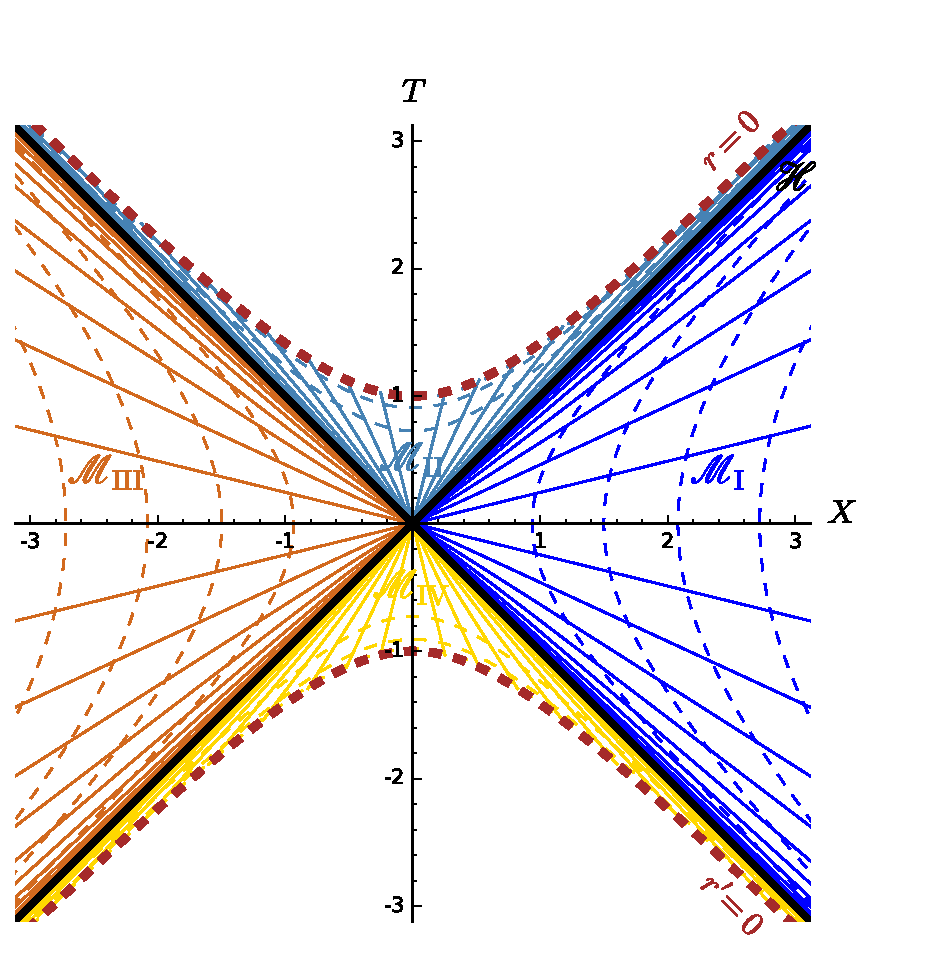
\includegraphics[width=0.6\textwidth]{sch_kruskal_diag.pdf}}
\caption[]{\label{f:sch:kruskal_diag} \footnotesize
\emph{Kruskal diagram:}
Schwarzschild spacetime $\M$ depicted in terms of Kruskal-Szekeres coordinates $(T,X)$.
Each point in this diagram, including the one at $(T,X)=(0,0)$,
is actually a sphere $\SS^2$, spanned by the
coordinates $(\th,\ph)$.
Solid lines denote the hypersurfaces $t=\mathrm{const}$ in $\M_{\rm I}$ and
$\M_{\rm II}$ and the  hypersurfaces $t'=\mathrm{const}$ in $\M_{\rm III}$ and
$\M_{\rm IV}$, whiles dashed curves
denote the hypersurfaces $r=\mathrm{const}$ in $\M_{\rm I}$ and
$\M_{\rm II}$ and the  hypersurfaces $r'=\mathrm{const}$ in $\M_{\rm III}$ and
$\M_{\rm IV}$.
The bifurcate Killing horizon is marked by thick black lines, while the
singularities at $r=0$ and $r'=0$ are depicted by the heavy dashed brown curve.}
\end{figure}

Let us define the following open subsets of $\M$, which are respectively
the images of $\M_{\rm I}$ and $\M_{\rm II}$ by the reflection through the origin
(\ref{e:sch:origin_reflection}):
\begin{subequations}
\label{e:max:range_TX_M_III_IV}
\begin{align}
 & \M_{\rm III}: \quad X < 0 \quad\mbox{and}\quad X < T < -X \\
 & \M_{\rm IV}: \quad - \sqrt{X^2+1} < T < -|X| .
\end{align}
\end{subequations}
On $\M_{\rm III}\cup \M_{\rm IV}$, one may introduce coordinates
$(t',r',\th,\ph)$ of Schwarzschild-Droste type; they are related to
the Kruskal-Szekeres coordinates by formulas analogous to
(\ref{e:sch:KS_SD_I}) and (\ref{e:sch:KS_SD_II}), simply changing $T$ to $-T$
and $X$ to $-X$:
\be \label{e:sch:KS_SD_III}
    \M_{\rm III}: \quad \encadre{ \left\{\begin{array}{l}
    T = - \mathrm{e}^{r'/4m} \sqrt{ \frac{r'}{2m} - 1 } \sinh\left( \frac{t'}{4m} \right)
\\[2ex]
    X = - \mathrm{e}^{r'/4m} \sqrt{ \frac{r'}{2m} - 1 } \cosh\left( \frac{t'}{4m} \right)
        \end{array}\right. }
    \iff
    \encadre{ \left\{\begin{array}{l}
    t' = 2 m \,  \ln \left( \frac{X+T}{X-T} \right) \\[2ex]
    r' = 2 m \tilde{W}_0(X^2 - T^2) .
        \end{array}\right. }
\ee
\be \label{e:sch:KS_SD_IV}
    \M_{\rm IV}: \quad \encadre{ \left\{\begin{array}{l}
    T = - \mathrm{e}^{r'/4m} \sqrt{ 1 - \frac{r'}{2m} } \cosh\left( \frac{t'}{4m} \right)
\\[2ex]
    X = - \mathrm{e}^{r'/4m} \sqrt{ 1 - \frac{r'}{2m} } \sinh\left( \frac{t'}{4m} \right)
        \end{array}\right. }
    \iff
    \encadre{ \left\{\begin{array}{l}
    t' = 2 m \,  \ln \left( \frac{T+X}{T-X} \right) \\[2ex]
    r' = 2 m \tilde{W}_0(X^2 - T^2) .
        \end{array}\right. }
\ee

The extended Schwarzschild spacetime $(\M,\w{g})$ is depicted in
Fig.~\ref{f:sch:kruskal_diag}, which is usually called a
\defin{Kruskal diagram}\index{Kruskal!diagram}.
There are two curvature singularities, which formally are not part of $\M$:
the hypersurfaces $r=0$ and $r'=0$.
As discussed in Sec.~\ref{s:sch:rad_null_geod_KS}, the radial null
geodesics appear as straight lines of slope $\pm 45^\circ$ ($+$ for the
outgoing family, and $-$ for the ingoing one).
As in $(\M_{\rm IEF},\w{g})$, they are still not complete but the only
locations where they terminate are the curvature singularities
at $r=0$ (future end point) and $r'=0$ (past end point). Therefore, they cannot
be extended further. For this reason, $(\M,\w{g})$ is called the
\defin{maximal extension}\index{maximal!extension}\index{extension!maximal --}
of Schwarzschild spacetime.

\begin{remark}
The extended manifold $\M$ is not just the union
$\M_{\rm I}\cup\M_{\rm II}\cup\M_{\rm III}\cup\M_{\rm IV}$, since the latter
does not cointain the hypersurfaces $T=\pm X$ (cf. the scrict inequalities
in Eqs.~(\ref{e:max:range_TX_M_I_II})
and (\ref{e:max:range_TX_M_III_IV})), which are parts of $\M$ according to
the definition (\ref{e:sch:def_M_extend}). Actually, we have
\be
    \M = \M_{\rm I}\cup\M_{\rm II}\cup\M_{\rm III}\cup\M_{\rm IV}\cup\hat{\Hor},
\ee
where $\hat{\Hor}$ is the bifurcate Killing horizon, to be discussed in
Sec.~\ref{s:max:bifur_Kill_hor}.
\end{remark}

\subsection{Global null coordinates} \label{s:max:glo_null}

In Secs.~\ref{s:sch:KS_coord} and \ref{s:sch:rad_null_geod_KS}, we have introduced
on $\M_{\rm IEF}$
the null coordinates $(U,V)$; they are related to the coordinates $(T,X)$
by Eq.~(\ref{e:sch:def_T_X}) (or equivalently
Eqs.~(\ref{e:sch:ingoing_null_geod_KS})-(\ref{e:sch:outgoing_null_geod_KS})),
which we case use define $(U,V)$ in all the maximal extension $\M$:
\be \label{e:max:U_V_T_X}
    \left\{\begin{array}{l}
    U = T - X\\
    V = T + X
    \end{array}\right.
    \qquad \iff\qquad
    \left\{\begin{array}{l}
    T = \frac{1}{2} (U+V) \\[1ex]
    X = \frac{1}{2} (V-U)
    \end{array}\right.
\ee
The range of $(U,V)$ of $\M$ is deduced from the constraint
$T^2-X^2 < 1$ [cf. Eq.~(\ref{e:sch:def_M_extend})]: since $T^2-X^2 = UV$,
we get:
\be \label{e:max:range_UV}
    \M:\quad (U,V)\in\R^2 \quad\mbox{and}\quad UV < 1.
\ee

The expression of the metric tensor
in terms of the null coordinates $x^\alpha = (U,V,\th,\ph)$
is deduced from (\ref{e:sch:metric_KS_TX}):
\be
    \encadre{
      g_{\mu\nu} \, \D x^\mu \, \D x^\nu = 4m^2 \left[
      \frac{4}{UV + \mathrm{e}^{\tilde{W}_0(-UV)} } \, \D U \, \D V
      + \tilde{W}_0(-UV)^2 \left( \D\th^2 + \sin^2\th\, \D\ph^2 \right) \right] .
    }
\ee
We can also rewrite it as (\ref{e:sch:metric_UV}):
\be \label{e:max:metric_UV_glob}
    \encadre{
    g_{\mu\nu} \, \D x^\mu \, \D x^\nu =
    - \frac{32 m^3}{r} \, \mathrm{e}^{-r/2m} \,  \D U \, \D V
     +  r^2 \left( \D\th^2 + \sin^2\th\, \D\ph^2 \right) },
\ee
where $r$ is the function of $(U,V)$ given by
\be \label{e:max:r_W0_UV}
    r = 2 m \tilde{W}_0(-UV) .
\ee
Note that the relation (\ref{e:max:r_UV_M_I}) between $r$ and $(U,V)$ holds
in all $\M$:
\be \label{e:max:r_UV}
    \encadre{ \mathrm{e}^{r/2m} \left( \frac{r}{2m} - 1 \right) = - U V } .
\ee

\begin{remark}
In Sec.~\ref{s:sch:max_extens_constr}, we have distinguished the
coordinate
$r$ in $\M_{\rm I}\cup \M_{\rm II}$ from the coordinate $r'$ in
$\M_{\rm III}\cup \M_{\rm IV}$. Here, $r$ is the function
(\ref{e:max:r_W0_UV}) of $(U,V)$, which has the same expression in
$\M_{\rm I}\cup \M_{\rm II}$ and $\M_{\rm III}\cup \M_{\rm IV}$. There is
no need to make any distinction. Hence there is no mention of $r'$
in (\ref{e:max:metric_UV_glob}).
\end{remark}


\begin{hist}
\label{n:max:KS_coord}
The Kruskal-Szekeres coordinates have been introduced in 1960 independently
by Martin D. Kruskal \cite{Krusk60} and George Szekeres \cite{Szeke60}.
Actually the coordinates
introduced by Szekeres were\footnote{They are denoted by $(v,u)$ in Szekeres' article \cite{Szeke60}.} $(2T/\sqrt{\mathrm{e}}, 2X/\sqrt{\mathrm{e}})$. Both Kruskal and Szekeres
have used these coordinates to construct the maximal  extension of Schwarzschild
spacetime. Its graphical representation in the $(X,T)$ plane (the
\emph{Kruskal diagram}\index{Kruskal!diagram}, cf. Fig.~\ref{f:sch:kruskal_diag}) has been presented by
Kruskal (Fig. 2 of Ref.~\cite{Krusk60}).
Actually, the maximal extension of Schwarzschild spacetime has been first constructed
by John L. Synge in 1950 \cite{Synge50}. He used coordinates\index{Synge!coordinates}
$(T',X')$
whose relation to
Schwarzschild-Droste coordinates is more complicated than the Kruskal-Szekeres one:
$T' = R(r) \sinh \left(\frac{t}{4m}\right)$
and $X' = R(r) \cosh \left(\frac{t}{4m}\right)$, with
$R(r) := 2m \left[ \mathrm{acosh}\sqrt{\frac{r}{2m}} + \sqrt{ \frac{r}{2m}\left(\frac{r}{2m} - 1 \right) }\right]$; compare with (\ref{e:sch:KS_SD_I}).
Albeit looking complicated, $R(r)$ is nothing but the primitive vanishing at
$r=2m$ of $r\mapsto \left(\frac{r}{2m} - 1 \right) ^{-1/2}$.
Interestingly, in his
article \cite{Szeke60}, Szekeres says that the transformations (\ref{e:sch:KS_SD_I})
``are essentially due to Synge'', probably because they differ only in the choice
of the function $R(r)$, the latter being
$R_{\rm KS}(r) = \mathrm{e}^{r/4m} \sqrt{r/2m-1}$ for Kruskal-Szekeres coordinates.
For this reason, both coordinate systems share some similarities: in Synge diagram\index{Synge!diagram} (Figs.~8 and 9 in Ref.~\cite{Synge50}),
the bifurcate horizon appears as the two bisector lines $T' = \pm X'$ and
the singularity $r=0$ as the hyperbola $T'^2 - X'^2 = \pi^2 m^2$ (compare with
$T^2-X^2 = 1$ for Kruskal-Szekeres coordinates). A major difference is that
Synge diagram is not ``conformal'': the radial null geodesics are generally not
lines with $\pm 45^\circ$ slope. Even, in some regions, the coordinate $T'$
ceases to be timelike\footnote{We refer the reader to Fig.~2 of Ref.~\cite{Unruh14}
for a plot of Synge coordinates in terms of Kruskal-Szekeres ones}.
The maximal extension of Schwarzschild spacetime
has also been found by Christian Fronsdal \cite{Frons59} in 1959, not via any explicit change of coordinates but rather via
an isometric embedding of the spacetime in the 6-dimensional Minkowski spacetime.
\end{hist}

%%%%%%%%%%%%%%%%%%%%%%%%%%%%%%%%%%%%%%%%%%%%%%%%%%%%%%%%%%%%%%%%%%%%%%%%%%%%%%%

\section{Bifurcate Killing horizon} \label{s:max:bifur_Kill_hor}

As discussed in Sec.~\ref{s:sch:max_extens}, the Schwarzschild horizon
$\Hor$ is
a non-degenerate Killing horizon and therefore shall be part of
a bifurcate Killing horizon (cf. Sec.~\ref{s:sta:bifur_Killing_hor})
in the extended spacetime.
The bifurcate Killing horizon, $\hat{\Hor}$ say, is easily found by
considering the Killing vector field $\w{\xi}$ in the maximal extension
of Schwarzschild spacetime. The components of $\w{\xi}$ w.r.t. to the
Kruskal-Szekeres coordinates are obtained from the
property $\w{\xi} = \wpar_t$:
\[
    \xi^T = \der{T}{t}, \quad
    \xi^X = \der{X}{t}, \quad
    \xi^\th = \der{\th}{t} = 0, \quad
    \xi^\ph = \der{\ph}{t} = 0 .
\]
Given the coordinate transformation laws (\ref{e:sch:KS_SD_I})
and (\ref{e:sch:KS_SD_II}), we get in
$\M_{\rm I}$ and $\M_{\rm II}$:
\[
    \xi^T = \frac{1}{4m} \, X, \quad
    \xi^X = \frac{1}{4m} \, T , \quad
    \xi^\th = \xi^\ph = 0 .
\]
Hence in $\M_{\rm I}\cup\M_{\rm II}$,
\be \label{e:sch:xi_X_T}
    \encadre{ \w{\xi} = \frac{1}{4m} \left( X \, \wpar_T + T \, \wpar_X \right) }.
\ee
Now, this formula defines a smooth vector field in all $\M$.
Moreover, in $\M_{\rm III}\cup\M_{\rm IV}$, this vector coincides with
$\wpar_{t'}$ since $\xi^T = \dert{T}{t'}$ and $\xi^X = \dert{X}{t'}$,
with the partial derivatives with respect to $t'$ evaluated from
(\ref{e:sch:KS_SD_III})-(\ref{e:sch:KS_SD_IV}). Hence the vector field
$\w{\xi}$ defined by (\ref{e:sch:xi_X_T}) is a Killing vector field
of maximal extension $(\M,\w{g})$. This vector field is depicted in
Fig.~\ref{f:sch:xi_extend}.

\begin{figure}
\centerline{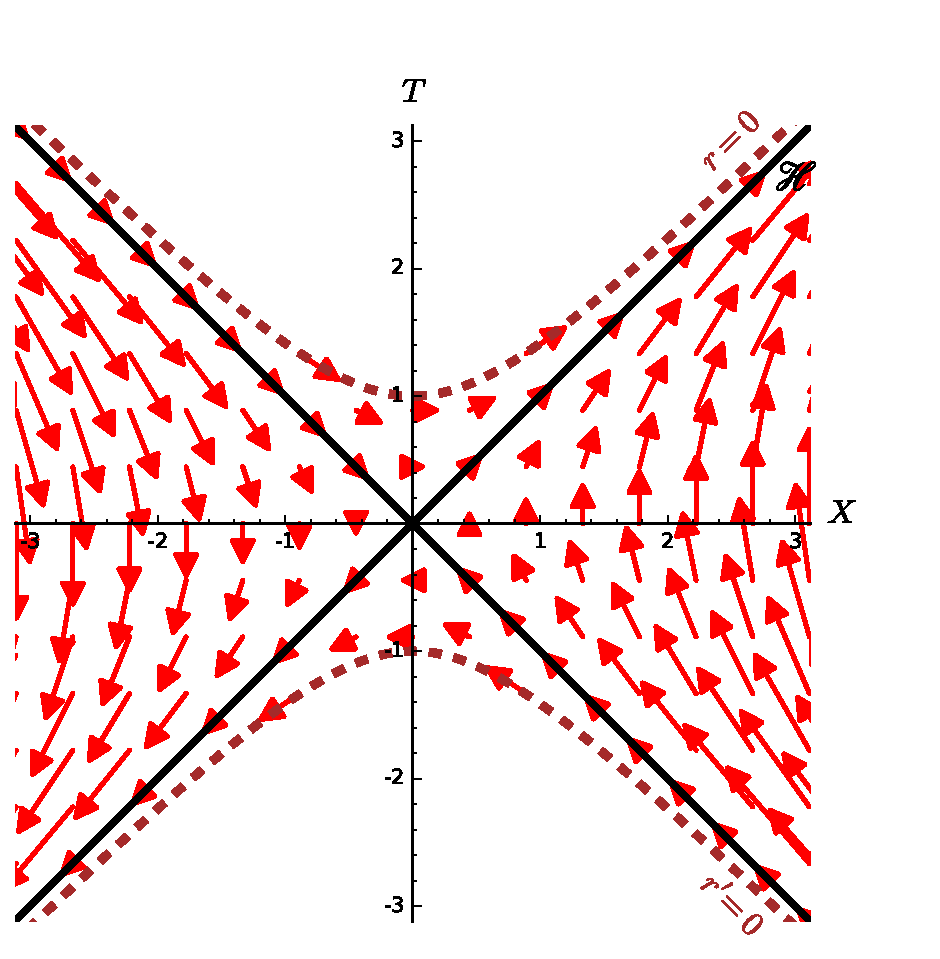
\includegraphics[width=0.6\textwidth]{sch_xi_extend.pdf}}
\caption[]{\label{f:sch:xi_extend} \footnotesize
Killing vector field $\w{\xi}$ on the extended Schwarzschild manifold.}
\end{figure}

The bifurcate Killing horizon with respect to $\w{\xi}$
that extends $\Hor$
is $\hat{\Hor} = \Hor_1 \cup \Hor_2 $, where
\begin{itemize}
\item $\Hor_1$ is the null hypersurface $T=X$ (or equivalently $U=0$);
\item $\Hor_2$ is the null hypersurface $T=-X$ (or equivalently $V=0$).
\end{itemize}
The bifurcate Killing horizon $\hat{\Hor}$ is depicted in black in
Fig.~\ref{f:sch:xi_extend}.
The Schwarzschild horizon $\Hor$ is the part of $\Hor_1$ defined by $X>0$.
In terms of the null coordinates $(U,V)$ introduced in Sec.~\ref{s:max:glo_null},
we have, given (\ref{e:max:U_V_T_X}),
\begin{subequations}
\label{e:max:Hor_U_V}
\begin{align}
    \hat{\Hor}:\quad&  U = 0 \quad\mbox{or}\quad V = 0 \\
    \Hor:\quad &   U = 0 \quad\mbox{and}\quad V > 0 .
\end{align}
\end{subequations}
The bifurcation surface is $\Sp = \Hor_1 \cap \Hor_2$, which
is the 2-surface defined by $T=0$ and $X=0$, or equivalently by
$U=0$ and $V=0$. It is a 2-sphere, since
any fixed value of the pair $(T,X)$ defines a 2-sphere, according to the
definition of $\M$ as a part of $\R^2\times\mathbb{S}^2$
[cf. Eq.~(\ref{e:sch:def_M_extend})]. Accordingly, $\Sp$ is called the
\defin{bifurcation sphere}\index{bifurcation!sphere}. It is located at the
center of Fig.~\ref{f:sch:xi_extend}.
The areal radius of $\Sp$ is found by setting
$\D T = 0$, $\D X = 0$ and $(T,X)=(0,0)$ in the line element
(\ref{e:sch:metric_KS_TX}):
\[
    r_{\Sp}^2 = 4m^2 \tilde{W}_0(0)^2.
\]
Since $\tilde{W}_0(0)=1$ (cf. Fig.~\ref{f:max:lambert_rescaled}), we get
\be
    \encadre{r_{\Sp} = 2 m } .
\ee
Moreover, setting $(T,X)=(0,0)$ in Eq.~(\ref{e:sch:xi_X_T}),
we recover the general property (\ref{e:sta:xi_S_zero}): the Killing
vector field vanishes at the bifurcation sphere:
\be
\left. \w{\xi} \right| _{\Sp} = 0 .
\ee

%%%%%%%%%%%%%%%%%%%%%%%%%%%%%%%%%%%%%%%%%%%%%%%%%%%%%%%%%%%%%%%%%%%%%%%

\section{Carter-Penrose diagram} \label{s:max:Carter-Penrose}

\subsection{First construction}

To have a compact representation of the maximal extension of Schwarzschild spacetime,
one can use the same trick as for Minkowski spacetime (cf. Sec.~\ref{s:glo:finite_range_Mink}), namely employ the arctangent function to map the
range $(-\infty, +\infty)$ of the null coordinates $U$ and $V$ to the
interval $(-\pi/2,\pi/2)$, thereby defining the finite-range coordinates
$(\hat{U},\hat{V})$:
\be \label{e:max:def_hUhV}
    \left\{ \begin{array}{l}
    \hat{U} = \arctan U \\
    \hat{V} = \arctan V
    \end{array} \right.
    \iff
   \left\{ \begin{array}{l}
    U = \tan \hat{U} \\
    V = \tan \hat{V} .
    \end{array} \right.
\ee
The range of $(\hat{U},\hat{V})$ is deduced from (\ref{e:max:range_UV}):
\[
    UV < 1 \iff \tan \hat{U} \,  \tan \hat{V} < 1 .
\]
Since for $\hat{U}, \hat{V}\in (-\pi/2,\pi/2)$, we have $\cos\hat{U} > 0$ and
$\cos\hat{V} > 0$, we may write
\[
    UV < 1 \iff  \sin\hat{U} \, \sin\hat{V} < \cos\hat{U} \, \cos\hat{V}
     \iff  \cos(\hat{U}+\hat{V}) > 0
     \iff  -\frac{\pi}{2} < \hat{U}+\hat{V} <\frac{\pi}{2} .
\]
Hence the range of $(\hat{U},\hat{V})$ on the maximal extension
of Schwarzschild spacetime:
\be \label{e:max:range_hUhV}
    \M:\quad -\frac{\pi}{2} < \hat{U} <\frac{\pi}{2},\quad
    -\frac{\pi}{2} < \hat{V} <\frac{\pi}{2}
    \quad\mbox{and}\quad -\frac{\pi}{2} < \hat{U}+\hat{V} <\frac{\pi}{2} .
\ee

Since (\ref{e:max:def_hUhV}) yields
$\D U = \D \hat{U} / \cos^2\hat{U}$ and $\D V = \D \hat{V} / \cos^2\hat{V}$,
we deduce immediately from (\ref{e:max:metric_UV_glob})
the expression of the metric tensor in terms of the coordinates
$x^\alpha = (\hat{U}, \hat{V}, \th,\ph)$:
\be \label{e:max:metric_hUhV}
    \encadre{
    g_{\mu\nu} \, \D x^\mu \, \D x^\nu =
    - \frac{32 m^3}{r} \, \mathrm{e}^{-r/2m} \,
        \frac{\D \hat{U}}{\cos^2\hat{U}} \, \frac{\D \hat{V}}{\cos^2\hat{V}}
     +  r^2 \left( \D\th^2 + \sin^2\th\, \D\ph^2 \right) },
\ee
where [cf. Eq.~(\ref{e:max:r_W0_UV})]
\be \label{e:max:r_hUhV}
    r = 2 m \tilde{W}_0(-\tan \hat{U} \tan \hat{V}) .
\ee

To depict $\M$, let us introduce  ``time+space'' coordinates $(\hat{T},\hat{X})$,
which are related to $(\hat{U},\hat{V})$ in exactly the same way
as the coordinates $(\tau,\chi)$ were related
to the finite-range null coordinates $(U,V)$ for Minkowski spacetime
[cf. Eq.~(\ref{e:glo:tau_chi_U_V})]:
\be \label{e:max:hThX_hUhV}
    \left\{ \begin{array}{l}
    \hat{T} = \hat{U} + \hat{V} \\
    \hat{X} = \hat{V} - \hat{U}
    \end{array} \right.
    \iff
    \left\{ \begin{array}{l}
    \hat{U} = \frac{1}{2} (\hat{T} - \hat{X}) \\[1ex]
    \hat{V} = \frac{1}{2} (\hat{T} + \hat{X}) .
    \end{array} \right.
\ee
The range of $(\hat{T},\hat{X})$ is deduced from (\ref{e:max:range_hUhV}):
\be \label{e:max:range_hThX}
    \M:\quad -\frac{\pi}{2} < \hat{T} <\frac{\pi}{2},\quad
        \hat{T}-\pi < \hat{X} < \hat{T}+\pi
    \quad\mbox{and}\quad -\hat{T}-\pi < \hat{X} < -\hat{T}+\pi.
\ee


Via (\ref{e:max:def_hUhV}) and (\ref{e:max:U_V_T_X}), the relation
between $(\hat{T},\hat{X})$ and the Kruskal-Szekeres coordinates $(T,X)$
is then the same as that between $(\tau,\chi)$ and $(t,r)$ for Minkowksi
spacetime [Eq.~(\ref{e:glo:tau_chi_t_r})]:
\be \label{e:max:tTtX}
    \left\{ \begin{array}{l}
    \hat{T} = \arctan(T+X) + \arctan(T-X) \\
    \hat{X} = \arctan(T+X) - \arctan(T-X)
    \end{array} \right.
    \iff
    \left\{ \begin{array}{l}
    \displaystyle T = \frac{\sin\hat{T}}{\cos\hat{T} + \cos\hat{X}}\\[2ex]
    \displaystyle X = \frac{\sin\hat{X}}{\cos\hat{T} + \cos\hat{X}} .
    \end{array} \right.
\ee

The maximal extension of Schwarzschild spacetime is depicted with respect
to the coordinates $(\hat{T},\hat{X})$ in Fig.~\ref{f:max:carter-penrose-std}.
Such a plot is called a \defin{Carter-Penrose diagram}\index{Carter-Penrose diagram}.
As the Kruskal diagram (Fig.~\ref{f:sch:kruskal_diag}), it has the property
to display the radial null geodesics as straight lines with slope $\pm 45^\circ$.
This holds
since $\hat{U}$ (resp. $\hat{V}$) is a function of $U$ only
(resp. $V$ only), cf. Eq.~(\ref{e:max:def_hUhV}), so that $\hat{U}$
(resp. $\hat{V}$) is constant on outgoing (resp. ingoing) radial null geodesics.
In particular, the bifurcate Killing horizon and the Schwarzschild horizon
are obtained for specific values of $\hat{U}$ and $\hat{V}$:
\begin{subequations}
\begin{align}
    \hat{\Hor}:\quad&  \hat{U} = 0 \quad\mbox{or}\quad \hat{V} = 0 \\
    \Hor:\quad &  \hat{U} = 0 \quad\mbox{and}\quad \hat{V} > 0 .
\end{align}
\end{subequations}
These relations follow immediately from (\ref{e:max:Hor_U_V}) and
(\ref{e:max:def_hUhV}).


\begin{figure}
\centerline{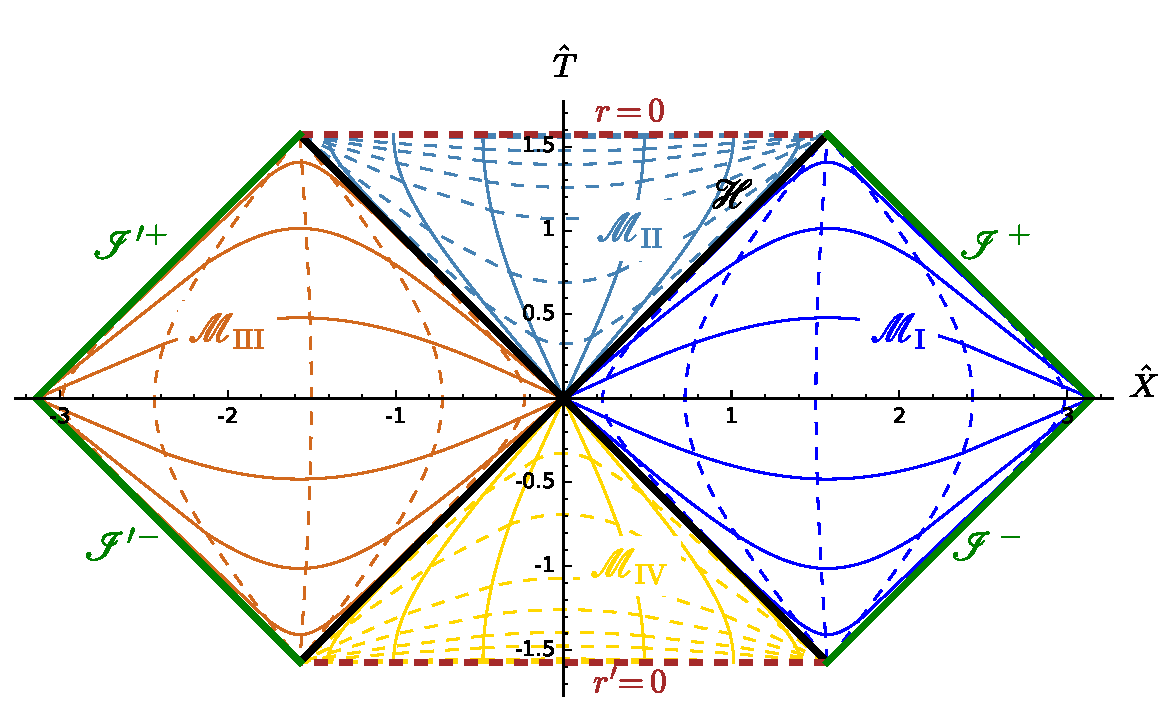
\includegraphics[width=0.9\textwidth]{max_carter-penrose-std.pdf}}
\caption[]{\label{f:max:carter-penrose-std} \footnotesize
Carter-Penrose diagram of the Schwarzschild spacetime
constructed with the compactified coordinates $(\hat{T},\hat{X})$.
Solid curves denote hypersurfaces of constant Schwarzschild-Droste coordinate
$t$: in region $\M_{\rm I}$, from the $\hat{X}$-axis to the top: $t=0$, $2m$,
$5m$, $10m$, $20m$ and $50m$, the last two being barely visible;
in region $\M_{\rm II}$, from the $\hat{T}$-axis
to the right: $t=0$, $2m$, $5m$, $10m$, $20m$ and $50m$,
Dashed curves denote hypersurfaces of constant Schwarzschild-Droste coordinate
$r$: in region $\M_{\rm I}$, from the left to the right: $r=2.01m$, $2.1m$, $2.5m$ (almost vertical), $4m$, $8m$, $12m$, $20m$ and $100m$, the last three being barely visible;
in region $\M_{\rm II}$, from the bottom to the top: $r=1.98m$, $1.9m$, $1.7m$,
$1.5m$, $1.25m$, $m$, $0.5m$ and $0.1m$.
The color code
is the same as in Fig.~\ref{f:sch:kruskal_diag}.
See Sec.~\ref{s:sam:std_Carter-Penrose} for the
SageManifolds worksheet generating this figure.}
\end{figure}


We have seen in Sec.~\ref{s:sch:BH} that the future null infinity $\scri^+$
corresponds to $v\rightarrow +\infty$ and that the past null infinity
$\scri^-$ to $u\rightarrow -\infty$ (cf. Fig.~\ref{f:sch:conf_compl_final}).
Since on $\M_{\rm I}$, $U = - \mathrm{e}^{-u/4m}$ and $V = \mathrm{e}^{v/4m}$
[cf. Eq.~(\ref{e:sch:def_U_V})], we
may write equivalently:
\begin{subequations}
\begin{align}
    \scri^+:&\quad V\rightarrow +\infty \quad\mbox{and}\quad U \in (-\infty, 0) \\
    \scri^-:&\quad U\rightarrow -\infty \quad\mbox{and}\quad V \in (0,+\infty) .
\end{align}
\end{subequations}
In view of (\ref{e:max:def_hUhV}), we get then:
\begin{subequations}
\label{e:max:scri_hUhV}
\begin{align}
    \scri^+:&\quad \hat{V}\rightarrow \frac{\pi}{2} \quad\mbox{and}\quad
        \hat{U} \in \left( -\frac{\pi}{2} , 0 \right) \\
    \scri^-:&\quad \hat{U}\rightarrow -\frac{\pi}{2} \quad\mbox{and}\quad
         \hat{V} \in \left( 0 ,  \frac{\pi}{2} \right).
\end{align}
\end{subequations}

By symmetry, the extension $\M_{\rm III}\cup \M_{\rm IV}$ of Schwarzschild
spacetime has the following null infinity:
\begin{subequations}
\label{e:max:scri_prime_hUhV}
\begin{align}
    {\scri'}^+:&\quad \hat{U}\rightarrow \frac{\pi}{2} \quad\mbox{and}\quad
        \hat{V} \in \left( -\frac{\pi}{2} , 0 \right) \\
    {\scri'}^-:&\quad \hat{V}\rightarrow -\frac{\pi}{2} \quad\mbox{and}\quad
        \hat{U}\in \left( 0 ,  \frac{\pi}{2} \right).
\end{align}
\end{subequations}

\subsection{Discussion: Carter-Penrose diagram and conformal completion}
\label{s:max:discus_hUhV}

The Carter-Penrose diagram in Fig.~\ref{f:max:carter-penrose-std} can be compared with the conformal diagram
of Minkowski spacetime in Fig.~\ref{f:glo:conf_diag_Mink}.
The right asymptotics of the Carter-Penrose diagram
(i.e. the part $\hat{X}>\pi/2$) looks similar to that of
Minkowski conformal diagram.
However, there is a difference: the coordinates $(\hat{T},\hat{X})$
employed in the construction of the diagram of
Fig.~\ref{f:max:carter-penrose-std} are not related to any (regular) conformal
completion --- as defined in Sec.~\ref{s:glo:conf_compl} ---
contrary to the coordinates $(\tau,\chi)$ used for Minkowski spacetime.

To see this, let us rewrite the metric components (\ref{e:max:metric_hUhV})
in a form that makes clear their behavior near null infinity. Given (\ref{e:max:r_hUhV}) and (\ref{e:max:exp_tW0}), we have
\be \label{e:max:exp_r_tUtV}
    \mathrm{e}^{r/2m} \left( \frac{r}{2m} - 1 \right) =
        -\tan \hat{U} \tan \hat{V} ,
\ee
from which we get
\[
    \frac{2m}{r} \mathrm{e}^{-r/2m} = - \frac{1-2m/r}{\tan \hat{U} \tan \hat{V}} .
\]
Hence
\[
    \frac{2m}{r} \frac{\mathrm{e}^{-r/2m}}{\cos^2\hat{U}\cos^2\hat{V}}
    =- \frac{1-2m/r}{\sin \hat{U} \cos\hat{U} \sin\hat{V}\cos\hat{V}}
   =  - \frac{4(1-2m/r)}{\sin 2\hat{U} \sin 2\hat{V}} .
\]
Therefore, we may rewrite expression~(\ref{e:max:metric_hUhV})
for the metric tensor as
\be \label{e:max:metric_hUhV_asymp}
    g_{\mu\nu} \, \D x^\mu \, \D x^\nu =
     64 m^2 \left( 1 - \frac{2m}{r} \right)\,
    \frac{\D \hat{U} \, \D \hat{V}}{\sin 2\hat{U} \sin 2\hat{V}}
     +  r^2 \left( \D\th^2 + \sin^2\th\, \D\ph^2 \right)  ,
\ee
with $r$ given by (\ref{e:max:r_hUhV}).
To get a conformal completion, we should write (cf. Sec.~\ref{s:glo:conf_compl})
\be \label{e:max:g_Omega2_tg}
    \w{g} = \Omega^{-2} \w{\tilde{g}} ,
\ee
where $\Omega = 0$ and $\dd\Omega \not=0$ on the spacetime boundary $\scri$ and
$\w{\tilde{g}}$ is a regular metric on the completion $\M\cup\scri$.
Since in Eq.~(\ref{e:max:metric_hUhV_asymp}), the term
$\sin 2\hat{U} \sin 2\hat{V}$ vanishes
at $\scri = \scri^+ \cup \scri^- \cup {\scri'}^+ \cup {\scri'}^-$
[cf. Eqs.~(\ref{e:max:scri_hUhV})-(\ref{e:max:scri_prime_hUhV})],
we would have, up to some constant factor,
\be \label{e:max:Omega_hUhV}
    \Omega = \sqrt{-\sin 2\hat{U} \sin 2\hat{V}} ,
\ee
the minus sign taking into account that
$\sin 2\hat{U} \sin 2\hat{V}$ approaches zero via negative values near
$\scri$.
A first issue is that the square root in (\ref{e:max:Omega_hUhV}) makes
$\Omega$ not differentiable on $\scri$, where either $\sin 2 \hat{U}=0$
or $\sin 2\hat{V}=0$. In other words, $\dd\Omega$ is diverging on $\scri$.
Suppose we accept this and are ready
to introduce a slight deviation (given that $\Omega^2$, which is involved in (\ref{e:max:g_Omega2_tg}), is smooth) from the definition given in
Sec.~\ref{s:glo:conf_compl}.
Then the conformal metric should be
\be \label{e:max:conf_metric_hUhV}
   {\tilde{g}}_{\mu\nu} \, \D x^\mu \, \D x^\nu =
     - 64 m^2 \left( 1 - \frac{2m}{r} \right)
    \D \hat{U} \, \D \hat{V}
     -  r^2 \sin 2\hat{U} \sin 2\hat{V}
     \left( \D\th^2 + \sin^2\th\, \D\ph^2 \right) .
\ee
Near $\scri$, $r\rightarrow +\infty$ and we have ${\tilde{g}}_{\hat{U}\hat{V}} \rightarrow -64 m^2$. On the contrary, ${\tilde{g}}_{\theta\theta}$ is
of the type ``$\infty\times 0$''; in order to determine its behaviour, let
us rewrite it as follows:
\[
    {\tilde{g}}_{\theta\theta} = -  r^2 \sin 2\hat{U} \sin 2\hat{V}
        = - 4 r^2 \sin\hat{U}\sin\hat{V} \times \cos\hat{U}\cos\hat{V},
\]
with $\cos\hat{U}\cos\hat{V}$ expressed via (\ref{e:max:exp_r_tUtV}):
\[
    \cos\hat{U}\cos\hat{V} = - \sin\hat{U} \sin\hat{V}
    \frac{\mathrm{e}^{-r/2m}}{r/2m - 1} .
\]
Hence
\[
    {\tilde{g}}_{\theta\theta} = 8 m \sin^2\hat{U} \sin^2\hat{V}
    \frac{ r \mathrm{e}^{-r/2m}}{1 - 2m/r}
\]
and (\ref{e:max:conf_metric_hUhV}) becomes
\be
   {\tilde{g}}_{\mu\nu} \, \D x^\mu \, \D x^\nu =
     - 64 m^2 \left( 1 - \frac{2m}{r} \right)
    \D \hat{U} \, \D \hat{V}
     + 8 m \sin^2\hat{U} \sin^2\hat{V}
    \frac{r \mathrm{e}^{-r/2m}}{1 - 2m/r}
     \left( \D\th^2 + \sin^2\th\, \D\ph^2 \right) .
\ee
On this expression, we can read directly the value of the conformal metric
at $\scri$,  where $r\rightarrow +\infty$, $2m/r \rightarrow 0$,
$r \mathrm{e}^{-r/2m}\rightarrow 0$ and
$\sin^2\hat{U}\rightarrow 1$ or
$\sin^2\hat{V}\rightarrow 1$:
\be \label{e:max:conf_metric_scri}
   {\tilde g}_{\mu\nu} \, \D x^\mu \, \D x^\nu
   \ \stackrel{\scri}{=}\  - 64 m^2 \D \hat{U} \, \D \hat{V} .
\ee
This bilinear form is clearly degenerate (cf. Sec.~\ref{s:bas:metric}).
Therefore $\w{\tilde{g}}$ is not a
regular metric on the whole manifold $\M\cup\scri$.
We conclude that (\ref{e:max:Omega_hUhV})-(\ref{e:max:conf_metric_hUhV}) does
not define a conformal completion of $(\M,\w{g})$.

\subsection{A regular conformal completion based on Frolov-Novikov coordinates}

In order to get a regular conformal completion of the maximally extended
Schwarzschild spacetime $(\M,\w{g})$, a finite-range coordinate system has
been proposed by Frolov \& Novikov \cite{FroloN98}: instead of (\ref{e:max:def_hUhV}),
the finite-range coordinates $(\tilde{U},\tilde{V})$ are defined in terms
of the null Kruskal-Szekeres coordinates $(U,V)$ by
\be \label{e:max:def_tUtV}
    \left\{ \begin{array}{l}
    \tilde{U} = \arctan(\mathrm{arsinh}\, U) \\
    \tilde{V} = \arctan(\mathrm{arsinh}\, V)
    \end{array} \right.
    \iff
   \left\{ \begin{array}{l}
    U = \sinh(\tan \tilde{U}) \\
    V = \sinh(\tan \tilde{V}) .
    \end{array} \right.
\ee
The range of $(\tilde{U},\tilde{V})$ is deduced from (\ref{e:max:range_UV}):
\be \label{e:max:range_tUtV}
    \M:\quad -\frac{\pi}{2} < \tilde{U} <\frac{\pi}{2},\quad
    -\frac{\pi}{2} < \tilde{V} <\frac{\pi}{2}
    \quad\mbox{and}\quad  \sinh(\tan \tilde{U}) \sinh(\tan \tilde{V}) < 1 .
\ee
Note that contrary to what happened for $(\hat{U},\hat{V})$, these conditions
do not yield to simple polygonal region in the $(\tilde{U},\tilde{V})$ plane.
The presence of the $\sinh$ function in the expression (\ref{e:max:def_tUtV}) of
$(U,V)$ in terms of $(\tilde{U},\tilde{V})$ does not alter the values
of the finite-range coordinates at null infinity, as compared to
$(\hat{U},\hat{V})$ [cf. (\ref{e:max:scri_hUhV})-(\ref{e:max:scri_prime_hUhV})]:
\begin{subequations}
\label{e:max:scri_tUtV}
\begin{align}
    \scri^+:&\quad \tilde{V}\rightarrow \frac{\pi}{2} \quad\mbox{and}\quad
        \tilde{U} \in \left( -\frac{\pi}{2} , 0 \right) \\
    \scri^-:&\quad \tilde{U}\rightarrow -\frac{\pi}{2} \quad\mbox{and}\quad
         \tilde{V} \in \left( 0 ,  \frac{\pi}{2} \right) \\
    {\scri'}^+:&\quad \tilde{U}\rightarrow \frac{\pi}{2} \quad\mbox{and}\quad
        \tilde{V} \in \left( -\frac{\pi}{2} , 0 \right) \\
    {\scri'}^-:&\quad \tilde{V}\rightarrow -\frac{\pi}{2} \quad\mbox{and}\quad
        \tilde{U}\in \left( 0 ,  \frac{\pi}{2} \right).
\end{align}
\end{subequations}
We shall call $(\tilde{U},\tilde{V},\th,\ph)$ the
\defin{Frolov-Novikov coordinates}\index{Frolov-Novikov coordinates}\index{coordinates!Frolov-Novikov --}.

From (\ref{e:max:def_tUtV}), we get
\[
    \D U = \frac{\cosh(\tan\tilde{U})}{\cos^2\tilde{U}}\, \D\tilde{U}
    \qquad\mbox{and}\qquad
    \D V = \frac{\cosh(\tan\tilde{V})}{\cos^2\tilde{V}}\, \D\tilde{V} ,
\]
so that the metric components in terms of the coordinates
$x^\alpha=(\tilde{U},\tilde{V},\th,\ph)$ are easily deduced from
(\ref{e:max:metric_UV_glob})-(\ref{e:max:r_W0_UV}):
\be \label{e:max:metric_tUtV}
    \encadre{
    g_{\mu\nu} \, \D x^\mu \, \D x^\nu =
    - \frac{32 m^3}{r} \, \mathrm{e}^{-r/2m} \,
        \frac{\cosh(\tan\tilde{U}) \cosh(\tan\tilde{V})}{\cos^2\tilde{U}\cos^2\tilde{V}}\,
            \D\tilde{U} \, \D\tilde{V}
     +  r^2 \left( \D\th^2 + \sin^2\th\, \D\ph^2 \right) },
\ee
where $r$ is the function of $(\tilde{U},\tilde{V})$ given by
\be \label{e:max:r_tUtV}
    r = 2 m \tilde{W}_0\!\left(-\sinh(\tan \tilde{U}) \sinh(\tan \tilde{V})\right) .
\ee
As we did for $(\hat{U},\hat{V})$, let us rewrite (\ref{e:max:metric_tUtV}) in
a form that is better adapted to the null asymptotics.
Given (\ref{e:max:r_tUtV}) and (\ref{e:max:exp_tW0}), we have
\be \label{e:max:exp_r_tUtV}
    \mathrm{e}^{r/2m} \left( \frac{r}{2m} - 1 \right) =
        - \sinh(\tan \tilde{U}) \sinh(\tan \tilde{V}) ,
\ee
from which we get
\[
    \frac{2m}{r} \mathrm{e}^{-r/2m} = - \left( 1 - \frac{2m}{r} \right)
        \frac{1}{\sinh(\tan \tilde{U}) \sinh(\tan \tilde{V})} .
\]
Hence (\ref{e:max:metric_tUtV}) becomes
\bea
    g_{\mu\nu} \, \D x^\mu \, \D x^\nu & =&
    16 m^2 \left( 1 - \frac{2m}{r} \right)
    \frac{\D\tilde{U} \, \D\tilde{V}}{\tanh(\tan\tilde{U}) \tanh(\tan\tilde{V}) \cos^2\tilde{U}\cos^2\tilde{V}} \nonumber\\
    & &
     +  r^2 \left( \D\th^2 + \sin^2\th\, \D\ph^2 \right) .
\eea
Given the values (\ref{e:max:scri_tUtV}) of $\tilde{U}$ and $\tilde{V}$ near
$\scri$, $\tanh(\tan\tilde{U}) \tanh(\tan\tilde{V})$ does not vanish there.
A natural choice of conformal factor is then
\be \label{e:max:def_Omega_tUtV}
   \encadre{ \Omega := \cos\tilde{U}\cos\tilde{V} }.
\ee
The corresponding conformal metric is
\be \label{e:max:conf_metric_tUtV}
    \encadre{
    \begin{array}{lcl}
    \displaystyle {\tilde g}_{\mu\nu} \, \D x^\mu \, \D x^\nu & =&
    \displaystyle 16 m^2 \left( 1 - \frac{2m}{r} \right)
    \frac{\D\tilde{U} \, \D\tilde{V}}{\tanh(\tan\tilde{U}) \tanh(\tan\tilde{V}) } \\[2ex]
    & &
     +  r^2 \cos^2\tilde{U}\cos^2\tilde{V} \left( \D\th^2 + \sin^2\th\, \D\ph^2 \right)
    \end{array} } .
\ee
Considering $(\tilde{U},\tilde{V},\th,\ph)$ as a canonical coordinate system
on $\R^2\times\SS^2$, we define the conformal completion manifold as
\bea
    \tilde{\M} &:= &\left\{ p\in \R^2\times\SS^2,\  (\tilde{U}(p),\tilde{V}(p)) \in \left( -\frac{\pi}{2}, \frac{\pi}{2} \right) ^2 \ \mbox{and}\
       \sinh(\tan \tilde{U}(p)) \sinh(\tan \tilde{V}(p)) < 1 \right\}
        \nonumber \\
       & & \cup \scri^+ \cup \scri^- \cup {\scri'}^+ \cup {\scri'}^- ,
        \label{e:max:def_M_compl}
\eea
with
\begin{subequations}\label{e:max:def_scri_R2S2}
\begin{align}
   \scri^+ := &\ \left\{ p\in \R^2\times\SS^2,\  \tilde{V}(p) = \frac{\pi}{2}
        \ \mbox{and}\ \tilde{U}(p) \in \left( -\frac{\pi}{2}, 0 \right) \right\}
            \label{e:max:def_scrip_R2S2} \\
    \scri^- := &\ \left\{ p\in \R^2\times\SS^2,\  \tilde{U}(p) = -\frac{\pi}{2}
        \ \mbox{and}\ \tilde{V}(p) \in \left( 0, \frac{\pi}{2}\right) \right\} \\
   {\scri'}^+ := &\ \left\{ p\in \R^2\times\SS^2,\  \tilde{U}(p) = \frac{\pi}{2}
        \ \mbox{and}\ \tilde{V}(p) \in \left( -\frac{\pi}{2}, 0 \right) \right\} \\
   {\scri'}^- := &\ \left\{ p\in \R^2\times\SS^2,\  \tilde{V}(p) = -\frac{\pi}{2}
        \ \mbox{and}\ \tilde{U}(p) \in \left( 0, \frac{\pi}{2}\right) \right\} .
\end{align}
\end{subequations}
Note that the first line in (\ref{e:max:def_M_compl}) corresponds to $\M$,
identified as a subset of $\R^2\times\SS^2$ [cf. Eq.~(\ref{e:max:range_tUtV})]
and that the definitions of $\scri^+$, $\scri^-$, ${\scri'}^+$ and ${\scri'}^-$
are in agreement with (\ref{e:max:scri_tUtV}). It is clear that $\tilde{\M}$
is a manifold with boundary and that
\be
    \partial\tilde{\M} = \scri := \scri^+ \cup \scri^- \cup {\scri'}^+
            \cup {\scri'}^- .
\ee
Moreover the scalar field $\Omega$ defined by (\ref{e:max:def_Omega_tUtV})
satisfies $\Omega \geq 0$ on $\tilde{\M}$, along with
$\Omega = 0$ on $\scri$ and $\dd\Omega\not = 0$ on $\scri$. The last property
follows from
\[
    \dd\Omega = -\sin\tilde{U} \cos\tilde{V}\, \dd\tilde{U}
            -\cos\tilde{U} \sin\tilde{V}\, \dd\tilde{V} ,
\]
which implies
$\left.\dd\Omega\right|_{\scri^+} = -\cos\tilde{U}\, \dd\tilde{V}\not=0$,
$\left.\dd\Omega\right|_{\scri^-} = \cos\tilde{V}\, \dd\tilde{U}\not=0$,
$\left.\dd\Omega\right|_{{\scri'}^+} = -\cos\tilde{V}\, \dd\tilde{U}\not=0$ and
$\left.\dd\Omega\right|_{{\scri'}^-} = \cos\tilde{U}\, \dd\tilde{V}\not=0$.
Hence the conditions 1, 3 and 4 of the definition of a conformal completion
given in Sec.~\ref{s:glo:conf_compl} are fulfilled. There remains to check
condition 2, namely that the tensor $\w{\tilde{g}}$ defined
by (\ref{e:max:conf_metric_tUtV}) is a regular metric on the whole $\tilde{\M}$.
This was the main failing point in the attempt of Sec.~\ref{s:max:discus_hUhV}.
Since $\Omega^2 > 0$ on $\M$, $\w{\tilde{g}}$ is well behaved on $\M$. Let us
thus examine its behaviour on $\scri$. We shall focus
on $\scri^+$, the behaviour on the other parts of $\scri$ being obtained by
some trivial symmetry. As one approaches $\scri^+$, $r\rightarrow +\infty$,
$\tilde{V}\rightarrow \pi/2$ and $\tanh(\tan(\tilde{V})\rightarrow 1$;
accordingly
we read from (\ref{e:max:conf_metric_tUtV}) that
\[
    \tilde{g}_{\tilde{U}\tilde{V}}
    \ \stackrel{\scri^+}{=}\  \frac{8 m^2}{\tanh(\tan\tilde{U})} \,
    \D\tilde{U} \, \D\tilde{V} .
\]
Besides, we have
$\tilde{g}_{\th\th} = r^2 \cos^2\tilde{U}\cos^2\tilde{V}$, which is of the type
``$+\infty \times 0$'' near $\scri^+$. Noticing that
$\tan\tilde{V}\sim 1/\cos\tilde{V}$ when $\tilde{V}\rightarrow \pi/2$, we get
from (\ref{e:max:exp_r_tUtV})
\[
    \sinh\left(\frac{1}{\cos\tilde{V}}\right) \sim - \frac{r \mathrm{e}^{r/2m}}{2m\sinh(\tan\tilde{U})}
        \quad \mbox{when} \quad \tilde{V}\rightarrow \frac{\pi}{2} .
\]
Since $\mathrm{arsinh}(x) = \ln(x + \sqrt{x^2+1}) \sim \ln x$ when $x\rightarrow +\infty$,
we obtain
\bea
    \frac{1}{\cos\tilde{V}} & \sim & \ln\left( - \frac{r \mathrm{e}^{r/2m}}{2m\sinh(\tan\tilde{U})} \right)
        = \frac{r}{2m} + \ln \left( \frac{r}{2m} \right) - \ln\left(-\sinh(\tan\tilde{U})\right) \nonumber \\
        & \sim & \frac{r}{2m} \quad \mbox{when} \quad \tilde{V}\rightarrow \frac{\pi}{2} .
            \nonumber
\eea
Hence $\cos^2\tilde{V} \sim 4m^2 / r^2$ and $\tilde{g}_{\th\th} \sim 4 m^2 \cos^2\tilde{U}$.
Gathering the above results, we have
\be
   {\tilde g}_{\mu\nu} \, \D x^\mu \, \D x^\nu
   \ \stackrel{\scri^+}{=}\  4 m^2 \left[
    \frac{4}{\tanh(\tan\tilde{U})} \, \D\tilde{U} \, \D\tilde{V}
        + \cos^2\tilde{U} \left( \D\th^2 + \sin^2\th\, \D\ph^2 \right) \right] .
\ee
Since $\cos^2\tilde{U} \not=0$ on $\scri^+$ [cf. Eq.~(\ref{e:max:def_scrip_R2S2})],
this bilinear form is non-degenerate.
Moreover, since $\tanh(\tan\tilde{U})<0$ on $\scri^+$ [again by (\ref{e:max:def_scrip_R2S2})], it has the
signature $(-,+,+,+)$.
 We conclude that $\w{\tilde{g}}$ is
a well behaved metric on the whole manifold $\tilde{\M}$. This completes the
demonstration that
\begin{greybox}
The pair
$(\tilde{\M},\w{\tilde{g}})$, with $\tilde{\M}$ defined by
(\ref{e:max:def_M_compl})-(\ref{e:max:def_scri_R2S2})
and $\w{\tilde{g}}$ defined by (\ref{e:max:conf_metric_tUtV}) is a conformal
completion of the maximally extented Schwarzschild spacetime $(\M,\w{g})$,
the conformal factor being given by (\ref{e:max:def_Omega_tUtV}).
The Frolov-Novikov coordinates $(\tilde{U},\tilde{V},\th,\ph)$ employed in this
construction are related to the null Kruskal-Szekeres coordinates $(U,V,\th,\ph)$
by (\ref{e:max:def_tUtV}).
\end{greybox}
\begin{remark}
At first sight, the metric $\w{\tilde{g}}$ given by (\ref{e:max:conf_metric_tUtV})
looks degenerate at the bifurcate Killing horizon $\Hor$, since $1-2m/r = 0$ there.
But one shall not forget that on $\Hor$, which is defined by
($\tilde{U}=0$ or $\tilde{V}=0$), one has $\tanh(\tan\tilde{U}) \tanh(\tan\tilde{V}) = 0$,
which compensate the vanishing of $1-2m/r$ in the term
${\tilde g}_{\tilde{U}\tilde{V}}$. Actually,
to deal with $\w{\tilde{g}}$ near $\Hor$, it is more appropriate
to use the form that is deduced from (\ref{e:max:metric_tUtV}) and (\ref{e:max:def_Omega_tUtV}):
\bea
    {\tilde g}_{\mu\nu} \, \D x^\mu \, \D x^\nu & =&
    - \frac{32 m^3}{r} \, \mathrm{e}^{-r/2m} \,
        \cosh(\tan\tilde{U}) \cosh(\tan\tilde{V}) \,
            \D\tilde{U} \, \D\tilde{V} \nonumber \\
    & & +  r^2 \cos^2\tilde{U}\cos^2\tilde{V}  \left( \D\th^2 + \sin^2\th\, \D\ph^2 \right) .
\eea
\end{remark}

\begin{remark}
The conformal completion constructed above cannot be analytically extended ``beyond'' $\scri$,
because the function $\tilde{V}\mapsto 1/\tanh(\tan\tilde{V})$, which appears in (\ref{e:max:conf_metric_tUtV}), is $C^\infty$ but not analytic at $\tilde{V}=\pi/2$.
It is possible to construct an analytic conformal completion, but it involves more
complicated coordinate transformations. The latter start,
not from the Kruskal-Szekeres coordinates
$(U,V)$, but from the null coordinates $(u,v)$ defined by (\ref{e:sch:u_v_r_t}).
We refer to the recent article \cite{HalacL14} for details.
\end{remark}

\begin{figure}
\centerline{\includegraphics[width=0.9\textwidth]{max_carter-penrose-FN.pdf}}
\caption[]{\label{f:max:carter-penrose-FN} \footnotesize
Carter-Penrose diagram of the Schwarzschild spacetime based on the Frolov-Novikov coordinates.
Solid curves denote the same hypersurfaces of constant Schwarzschild-Droste coordinate
$t$ as in Fig.~\ref{f:max:carter-penrose-std}: in region $\M_{\rm I}$, from the $\hat{X}$-axis to the top: $t=0$, $2m$,
$5m$, $10m$, $20m$ and $50m$;
in region $\M_{\rm II}$, from the $\hat{T}$-axis
to the right: $t=0$, $2m$, $5m$, $10m$, $20m$ and $50m$,
Dashed curves denote the same hypersurfaces of constant Schwarzschild-Droste coordinate
$r$ as in Fig.~\ref{f:max:carter-penrose-std}: in region $\M_{\rm I}$, from the left to the right: $r=2.01m$, $2.1m$, $2.5m$, $4m$, $8m$, $12m$, $20m$ and $100m$;
in region $\M_{\rm II}$, from the bottom to the top: $r=1.98m$, $1.9m$, $1.7m$,
$1.5m$, $1.25m$, $m$, $0.5m$ and $0.1m$.
The color code
is the same as in Figs.~\ref{f:sch:kruskal_diag} and \ref{f:max:carter-penrose-std}.
Contrary to the Carter-Penrose of Fig.~\ref{f:max:carter-penrose-std}, this one is
associated to a regular conformal completion at null infinity of Schwarzschild spacetime. See Sec.~\ref{s:sam:reg_Carter-Penrose} for the
SageManifolds worksheet generating this figure.}
\end{figure}



To depict $\tilde{\M}$, let us introduce ``time+space'' coordinates
$(\tilde{T},\tilde{X})$,
which are related to $(\hat{U},\hat{V})$ in exactly the same way
as $(\hat{T},\hat{X})$ are related to $(\hat{U},\hat{V})$
[cf. Eq.~(\ref{e:max:hThX_hUhV})]:
\be \label{e:max:tTtX_tUtV}
    \left\{ \begin{array}{l}
    \tilde{T} = \tilde{U} + \tilde{V} \\
    \tilde{X} = \tilde{V} - \tilde{U}
    \end{array} \right.
    \iff
    \left\{ \begin{array}{l}
    \tilde{U} = \frac{1}{2} (\tilde{T} - \tilde{X}) \\[1ex]
    \tilde{V} = \frac{1}{2} (\tilde{T} + \tilde{X}) .
    \end{array} \right.
\ee
The range of $(\tilde{T},\tilde{X})$ is deduced from (\ref{e:max:range_tUtV}):
\bea
    \M:& &  -\pi < \tilde{T} - \tilde{X} <\pi,\quad
    -\pi < \tilde{T} + \tilde{X} < \pi \nonumber \\
    & &  \sinh[\tan((\tilde{T}-\tilde{X})/2)]
        \; \sinh[\tan((\tilde{T}+\tilde{X})/2)] < 1 . \label{e:max:range_tTtX}
\eea
The picture of $(\M,\w{g})$ in the $(\tilde{T},\tilde{X})$ plane is shown in
Fig.~\ref{f:max:carter-penrose-FN}. We shall call it a
\defin{regular Carter-Penrose diagram}\index{Carter-Penrose diagram!regular --}
of Schwarzschild spacetime.
As the singular Carter-Penrose diagram of Fig.~\ref{f:max:carter-penrose-std},
it has the property
to display the radial null geodesics as straight lines with slope $\pm 45^\circ$,
since $\tilde{U}$ (resp. $\tilde{V}$) is a function of $U$ only
(resp. $V$ only) [cf. Eq.~(\ref{e:max:def_tUtV})].
In particular, the bifurcate Killing horizon and the Schwarzschild horizon
are defined by:
\begin{subequations}
\begin{align}
    \hat{\Hor}:\quad&  \tilde{U} = 0 \quad\mbox{or}\quad \tilde{V} = 0 \ \iff \
    \tilde{T} = \tilde{X} \quad\mbox{or}\quad \tilde{T} = - \tilde{X} \\
    \Hor:\quad &  \tilde{U} = 0 \quad\mbox{and}\quad \tilde{V} > 0 \ \iff \
      \tilde{T} = \tilde{X} \quad\mbox{and}\quad \tilde{T} > 0 .
\end{align}
\end{subequations}
These relations follow immediately from (\ref{e:max:Hor_U_V}),
(\ref{e:max:def_tUtV}) and (\ref{e:max:tTtX_tUtV}).


At first sight, the main difference with the ``standard'' Carter-Penrose diagram
of Fig.~\ref{f:max:carter-penrose-std} is the more complicated shape of
the boundary around the $\tilde{T}$-axis. This follows from the third
condition in (\ref{e:max:range_tTtX}), which is more involved than
the third condition in (\ref{e:max:range_hThX}).
Actually this boundary corresponds to the curvature singularity limit $r\rightarrow 0$
or $r'\rightarrow 0$. Indeed, from Eq.~(\ref{e:max:r_UV}), we have
\be \label{e:max:r_zero_UV}
    r = 0 \iff UV = 1 .
\ee
In terms of the coordinates $(\hat{U},\hat{V})$, we have then
[cf. Eq.~(\ref{e:max:def_hUhV})]
\bea
    r = 0 &\iff & \tan \hat{U} \tan \hat{V} = 1 \iff \sin \hat{U} \cos \hat{V} =
    \cos\hat{U} \cos\hat{V} \nonumber \\
    &\iff & \cos\hat{U} \cos\hat{V} - \sin \hat{U} \cos \hat{V} = 0
     \iff \cos(\hat{U} + \hat{V}) = 0
     \iff \hat{U} + \hat{V} = \pm \frac{\pi}{2} .  \nonumber
\eea
Since $\hat{T} = \hat{U} + \hat{V}$, we get the simple relation
\be
    r = 0 \iff \hat{T} =  \pm \frac{\pi}{2} .
\ee
On the contrary, in terms of the coordinates $(\tilde{U},\tilde{V})$,
Eq.~(\ref{e:max:r_zero_UV}) becomes [cf.
Eq.~(\ref{e:max:def_tUtV})]
\[
    r = 0 \iff \sinh(\tan \tilde{U}) \sinh(\tan \tilde{V}) = 1 ,
\]
which yields to the complicated formula
\be \label{e:max:r_zero_tTtX}
    r = 0 \iff  \sinh[\tan((\tilde{T}-\tilde{X})/2)]
        \; \sinh[\tan((\tilde{T}+\tilde{X})/2)] = 1 .
\ee
This explains the more complex boundary of Fig.~\ref{f:max:carter-penrose-FN}
diagram with respect to Fig.~\ref{f:max:carter-penrose-std} diagram.

\begin{remark}
The shape of the Carter-Penrose diagram in Frolov \& Novikov's book (Fig.~5.2 of
Ref.~\cite{FroloN98}; see also Fig.~10.6 of Ref.~\cite{FroloZ11}) differs slightly from the diagram obtained here (Fig.~\ref{f:max:carter-penrose-FN}). This is because
the coordinates used by Frolov \& Novikov are constructed from the
Szekeres' version (up to a factor 2) of Kruskal-Szekeres coordinates:
$T' = T/\sqrt{e}$ and $X'=X/\sqrt{e}$
(cf. the historical note on p.~\pageref{n:max:KS_coord}).
Accordingly, in Frolov \& Novikov's version, one shall replace the $1$
in the right-hand side of Eq.~(\ref{e:max:r_zero_tTtX}) by $1/e$, yielding to
a different shape of the boundary $r=0$.
\end{remark}

\begin{remark}
As noticed by Frolov and Novikov \cite{FroloN98} (see their Sec.~5.1.3),
one can perform some
coordinate transformation from $(\tilde{U},\tilde{V})$ to get a
Carter-Penrose diagram with a straight line for the boundary $r=0$.
\end{remark}

Besides the shape of the boundary $r=0$, another difference between
the Carter-Penrose diagram based on Frolov-Novikov coordinates
(Fig.~\ref{f:max:carter-penrose-FN}) and the ``standard'' diagram
of Fig.~\ref{f:max:carter-penrose-std} is that the $t=\mathrm{const}$
hypersurfaces of the former (solid curves in Fig.~\ref{f:max:carter-penrose-FN})
are all tangent to the horizontal axis when $\tilde{X}\rightarrow \pm\pi$.
On the contrary, the same hypersurfaces in Fig.~\ref{f:max:carter-penrose-std}
reach the point $(\hat{T},\hat{X}) = (0,\pm\pi)$ with a finite slope.
We note that in this respect, the Carter-Penrose diagram of
Fig.~\ref{f:max:carter-penrose-FN} is similar to the conformal diagram of
Minkowski spacetime, as shown in Fig.~\ref{f:glo:conf_diag_Mink}, and
therefore display correctly the asymptotic flatness structure.
The failure of diagram of Fig.~\ref{f:max:carter-penrose-std} to reproduce
this behavior reflects the fact that the coordinates $(\hat{T},\hat{X})$ are singular on the
boundary, as discussed in Sec.~\ref{s:max:discus_hUhV}.

\begin{figure}
\centerline{\includegraphics[width=0.6\textwidth]{max_constant_T_slices.pdf}}
\caption[]{\label{f:max:constant_T_slices} \footnotesize
Kruskal diagram with the hypersurfaces $\Sigma_{T_0}$ (defined by $T=T_0 = \mathrm{const.}$) as blue horizontal lines. For $|T_0|>1$, the dotted part of
$\Sigma_{T_0}$ corresponds to a region that cannot be embedded isometrically in
the Euclidean space. When $T_0$ varies, the limit of these regions form
the grey dotted curve.}
\end{figure}

%%%%%%%%%%%%%%%%%%%%%%%%%%%%%%%%%%%%%%%%%%%%%%%%%%%%%%%%%%%%%%%%%%%%%%%%%%%%%%%%%%%%%

\section{Einstein-Rosen bridge}

\subsection{Hypersurfaces of constant Kruskal-Szekeres time} \label{s:max:hyp_const_T}

To get some insight on the maximally extended Schwarzschild
spacetime $(\M,\w{g})$, let us examine the geometry of a slice of constant
Kruskal-Szekeres time $T$, i.e. a hypersurface $\Sigma_{T_0}$ defined
in terms of the global Kruskal-Szekeres coordinates $(T,X,\th,\ph)$ by
$T=T_0$, where $T_0\in\mathbb{R}$ is a constant
(cf. Fig.~\ref{f:max:constant_T_slices}).
The 3-uple $(x^i)=(X,\th,\ph)$ is then a coordinate system on $\Sigma_{T_0}$
subject to the constraint expressed in (\ref{e:sch:def_M_extend}):
\be
    X^2 > T_0^2 - 1 .
\ee
Consequently
\begin{itemize}
\item if $|T_0|< 1$, the hypersurface $\Sigma_{T_0}$ is connected
and diffeomorphic to $\R\times\SS^2$, the coordinate $X$ spanning $\R$ and
$(\th,\ph)$ spanning $\SS^2$.
\item if $|T_0| \geq 1$, $\Sigma_{T_0}$ has two connected components,
defined by
$X < - \sqrt{T_0^2 - 1}$ and $X > \sqrt{T_0^2 - 1}$ respectively
(cf. Fig.~\ref{f:max:constant_T_slices}).
Each of them is diffeomorphic to $\R\times\SS^2$.
\end{itemize}
For future convenience, we split $\Sigma_{T_0}$ in two disjoint parts, according
to the sign of $X$:
\be
    \Sigma^+_{T_0} = \left\{ p \in \Sigma_{T_0},\quad X(p) \geq 0 \right\}
    \quad\mbox{and}\quad
    \Sigma^-_{T_0} = \left\{ p \in \Sigma_{T_0},\quad X(p) < 0 \right\} .
\ee
For $|T_0|< 1$, there is a slight asymmetry between the
two parts: $\Sigma^+_{T_0}$ is a manifold with boundary
(cf. Sec.~\ref{s:bas:manif_boundary}), the boundary corresponding
to $X=0$, while $\Sigma^-_{T_0}$ is not.
For $|T_0|\geq 1$, $\Sigma^+_{T_0}$ and $\Sigma^-_{T_0}$ are nothing but the
two connected components of $\Sigma_{T_0}$.

The geometry of $\Sigma_{T_0}$ is defined by the metric $\w{\gamma}$
induced on it by $\w{g}$:
\be \label{e:max:gam_induced}
    \gamma_{ij} \D x^i \D x^j =
    \frac{32 m^3}{r} \, \mathrm{e}^{-r/2m} \,  \D X^2
     +  r^2 \left( \D\th^2 + \sin^2\th\, \D\ph^2 \right) ,
\ee
where $r$ is the function of $X$ defined by
\be \label{e:max:Sigma0_r_X}
    r = r(X) = 2 m  \tilde{W}_0(X^2 - T_0^2) .
\ee
The line element (\ref{e:max:gam_induced}) is obtained by setting $T=T_0$ and
$\D T = 0$ in (\ref{e:sch:metric_KS_TX}).
Since $r>0$, the metric (\ref{e:max:gam_induced}) is clearly positive definite,
i.e. $\w{\gamma}$ is a Riemannian metric and $\Sigma_{T_0}$ is a
spacelike hypersurface.

The graph of the function $r(X)$ is shown in Fig.~\ref{f:max:SigmaT0_r_X}.
Once restricted to positive (resp. negative) values of $X$, this function is a bijection
$(X_0, +\infty)\rightarrow (r_0, +\infty)$ (resp. $(-\infty, -X_0)\rightarrow (r_0, +\infty)$), where
\be \label{e:max:def_X0_r0}
    X_0 = \left\{ \begin{array}{ll}
        0 & \ \mbox{if}\quad  |T_0| < 1 \\
        \sqrt{T_0^2-1} & \ \mbox{if}\quad  |T_0| \geq 1.
        \end{array} \right.
    \quad \mbox{and}\quad
    r_0 = \left\{ \begin{array}{ll}
        2m \tilde{W}_0(-T_0^2) & \ \mbox{if}\quad  |T_0| < 1 \\
        0 & \ \mbox{if}\quad  |T_0| \geq 1.
        \end{array} \right.
\ee
The inverse of this bijection is\footnote{Let us recall that
$\tilde{W}_0^{-1}(x) = \mathrm{e}^x (x-1)$.}
\be \label{e:max:Sigma0_X_r}
    X = X(r) = \pm \sqrt{\mathrm{e}^{r/2m} \left( \frac{r}{2m} - 1 \right) + T_0^2} ,
\ee
with the $+$ sign on $\Sigma^+_{T_0}$ and the $-$ sign
on $\Sigma^-_{T_0}$.

\begin{figure}
\centerline{\includegraphics[height=0.35\textheight]{max_SigmaT0_r_X.pdf}}
\caption[]{\label{f:max:SigmaT0_r_X} \footnotesize
Function $r = r(X)$ on the hypersurface $\Sigma_{T_0}$, for the same values
of $T_0$ as in Fig.~\ref{f:max:constant_T_slices}.}
\end{figure}

We may use the above bijection to introduce coordinates $(r,\th,\ph)$ instead of $(X,\th,\ph)$
on each of the two regions $\Sigma^+_{T_0}$ and $\Sigma^-_{T_0}$.
Differentiating (\ref{e:max:Sigma0_X_r}) leads to
\[
    \D X = \pm \frac{r \mathrm{e}^{r/2m}}{8m^2 \sqrt{\mathrm{e}^{r/2m} \left( \frac{r}{2m} - 1 \right) + T_0^2}} \, \D r .
\]
Substituting in (\ref{e:max:gam_induced}) we get the expression of the
metric on $\Sigma_{T_0}$ in terms of the coordinates $(x^i) = (r,\th,\ph)$:
\be \label{e:max:Sigma0_metric}
    \gamma_{ij}\,  \D x^i \D x^j = \left(
    1 - \frac{2m}{r} \left(1 -  T_0^2 \mathrm{e}^{-r/2m} \right) \right) ^{-1} \, \D r^2
     +  r^2 \left( \D\th^2 + \sin^2\th\, \D\ph^2 \right) .
\ee
\begin{remark} \label{r:max:check_metric_SigmaT0}
As a check of the above formula, we notice that for $T_0=0$ it reduces to the
metric of a slice $t=\mathrm{const}$ in Schwarzschild-Droste coordinates
[set $\D t =0$ in Eq.~(\ref{e:sch:Schwarz_metric_SD})]. This is correct since
the positive-$X$ half of the hypersurface $T=0$ in Kruskal-Szekeres coordinates,
i.e. $\Sigma_0^+$,
coincides with the hypersurface $t=0$ in Schwarzschild-Droste coordinates,
as it can be seen by setting $T=0$ in Eq.~(\ref{e:sch:KS_SD_I})
(see also Fig.~\ref{f:max:constant_T_slices}).
\end{remark}

\subsection{Isometric embedding in 3-dimensional Euclidean space}

We may visualize the geometry of the spacelike hypersurface $\Sigma_{T_0}$
via some isometric embedding of some 2-dimensional slice of it
in the 3-dimensional Euclidean space $(\R^3, \w{f})$, $\w{f}$ being the standard
flat (Euclidean) metric.
By \defin{isometric embedding}\index{isometric!embedding}\index{embedding!isometric --}
of a 2-dimensional Riemannian manifold $(\Sp,\w{g})$
in $(\R^3,\w{f})$, it is meant a \emph{smooth embedding} $\Phi:\ \Sp \rightarrow \R^3$,
as defined in Sec.~\ref{s:bas:embed},
such that the metric induced on $\Phi(\Sp)$ by the Euclidean metric of $\R^3$
coincides with the original metric $\w{g}$ on $\Sp$:
\be \label{e:max:isometric_emb}
    \forall p\in \Sp,\quad  \forall (\w{u},\w{v})\in (T_p \Sp)^2,\quad
        \w{f}(\Phi^*(\w{u}), \Phi^*(\w{v})) = \w{g}(\w{u},\w{v}) ,
\ee
where $\Phi^*(\w{u})$ is the ``image of the vector $\w{u}$ by $\Phi$'', i.e.
the pushforward of $\w{u}$ by $\Phi$, as defined in
Sec.~\ref{s:bas:Lie_der_vector}. Another phrasing of the
isometry property (\ref{e:max:isometric_emb}) is: the pullback of $\w{f}$
on $\Sp$ by $\Phi$ coincides with $\w{g}$: $\Phi^*\w{f} = \w{g}$ [cf. Eq.~(\ref{e:bas:def_pullback})].

Taking into account the spherical symmetry
of $\Sigma_{T_0}$, there is no loss of generality in choosing the
equatorial plane $\theta=\pi/2$ as the 2-dimensional slice. We shall denote
it by $\Sigma_{T_0}^{\rm eq}$.
Coordinates on $\Sigma_{T_0}^{\rm eq}$ are $(x^a)=(X,\ph)$, or
on each of the two parts $\Sigma_{T_0}^{+,\rm eq}$ ($X\geq 0$) and
$\Sigma_{T_0}^{-,\rm eq}$ ($X<0$),
$(x^a)=(r,\ph)$.
If $|T_0| < 1$, the topology of $\Sigma_{T_0}^{\rm eq}$ is
$\R\times\SS^1$, i.e. that of a cylinder, while for $|T_0| \geq 1$, it has
two connected components, $\Sigma_{T_0}^{+,\rm eq}$ and
$\Sigma_{T_0}^{-,\rm eq}$, each of them having the topology of a cylinder.

The metric induced by $\w{g}$
on $\Sigma_{T_0}^{\rm eq}$,
$\w{q}$ say, is obtained by setting $\th=\pi/2$ and $\D\th=0$ in
Eq.~(\ref{e:max:Sigma0_metric}):
\be \label{e:max:metric_q}
    q_{ab}\,  \D x^a \D x^b = \left(
    1 - \frac{2m}{r} \left(1 -  T_0^2 \mathrm{e}^{-r/2m} \right) \right) ^{-1}
     \, \D r^2 +  r^2 \D\ph^2 .
\ee
Given the invariance in $\ph$, it is
quite natural to embed $(\Sigma_{T_0}^{\rm eq},\w{q})$ as
a surface of revolution in the Euclidean space $(\R^3, \w{f})$.
Describing $\R^3$ with cylindrical coordinates $(x^i) = (r,z,\ph)$,
the Euclidean metric $\w{f}$ is
\be
    f_{ij}\,  \D x^i \D x^j = \D r^2 + \D z^2 + r^2 \D\ph^2 .
\ee
A surface of revolution $\Sp$ in $\R^3$ is described by an equation of the type
$z = Z(r)$. On such a surface, one has therefore
$\D z = Z'(r) \, \D r$, so that the metric $\w{h}$ induced by $\w{f}$ on it is
\be \label{e:max:metric_h}
    h_{ab}\,  \D x^a \D x^b = \left( 1 + Z'(r)^2 \right) \D r^2
            + r^2 \D\ph^2 .
\ee
Comparing (\ref{e:max:metric_h}) with (\ref{e:max:metric_q}),
we see that a possible isometric embedding of $\Sigma_{T_0}^{\rm eq}$ into $\R^3$
is
\be \label{e:max:def_embedding_Phi}
    \begin{array}{clcl}
    \Phi: & \Sigma_{T_0}^{\rm eq} & \longrightarrow & \R^3 \\
        & (X,\ph) & \longmapsto & (r,z,\ph) = \left(r(X), \pm Z(r(X)), \ph \right) ,
    \end{array}
\ee
with (i) the sign $\pm$ being $+$ on $\Sigma_{T_0}^{+,\rm eq}$ and $-$ on
$\Sigma_{T_0}^{-,\rm eq}$ and (ii) the function $Z$ obeying
\[
   1 + Z'(r)^2 =  \left(
    1 - \frac{2m}{r} \left(1 -  T_0^2 \mathrm{e}^{-r/2m} \right) \right) ^{-1} .
\]
Thanks to Eq.~(\ref{e:max:Sigma0_X_r}), this expression can be recast as
\be \label{e:max:Zp2}
    Z'(r)^2 = \frac{1 - T_0^2  \mathrm{e}^{-r/2m}}{
    T_0^2  \mathrm{e}^{-r/2m} + \frac{r}{2m} - 1} =
    \frac{\mathrm{e}^{r/2m} - T_0^2}{X(r)^2} .
\ee
For $|T_0|<1$, i.e. when $\Sigma_{T_0}^{\rm eq}$ is connected, the
map (\ref{e:max:def_embedding_Phi}) defines a smooth embedding if, and only
if, at the boundary $X=0$ between $\Sigma_{T_0}^{+,\rm eq}$ and
$\Sigma_{T_0}^{-,\rm eq}$, the following holds:
\be
    Z(r(0)) = 0 \quad\mbox{and}\quad Z'(r(0)) = \infty .
\ee
The condition $Z(r(0)) = 0$ insures the continuity of the embedded surface
$\Phi(\Sigma_{T_0}^{\rm eq})$,
while $Z'(r(0)) = +\infty$ insures that it has a vertical tangent at
the junction between $\Phi(\Sigma_{T_0}^{+,\rm eq})$ and
$\Phi(\Sigma_{T_0}^{-,\rm eq})$, so that it is
a smooth surface. Fortunately, the condition $Z'(r(0)) = \infty$
is automatically fulfilled from the second expression of
$Z'(r)^2$ in (\ref{e:max:Zp2}): $Z'(r)^2$ clearly diverges at $X=0$.
Moreover, in order for the isometric embedding $\Phi$ to be well defined, the right-hand side
of (\ref{e:max:Zp2}) must be non-negative. Since the denominator of the last
term is manifestly non-negative, the sign is determined by the numerator. Hence
the condition $\mathrm{e}^{r/2m} \geq T_0^2$, or equivalently,
\be \label{e:max:cond_r_embed}
    r \geq 4 m \ln |T_0| .
\ee
For $|T_0|\leq 1$, this condition is always fulfilled, since $\ln |T_0| \leq 0$
and $r \geq 0$. For $|T_0| > 1$, it implies the existence of a minimal value
of $r$,
\be \label{e:max:r_emb}
    r_{\rm emb}(T_0) :=  4 m \ln |T_0|,
\ee
such that the part of $\Sigma_{T_0}^{\rm eq}$ with $r< r_{\rm emb}(T_0)$
cannot be embedded isometrically in the Euclidean 3-space.
\begin{remark}
The above result should not be surprising since there is
no guarantee that a 2-dimensional Riemannian manifold can
be isometrically embedded in the 3-dimensional Euclidean space.
The relevant theorem here is \emph{Nash embedding theorem}\index{Nash embedding theorem}\index{embedding!Nash -- theorem} \cite{Nash56}, which
states that any smooth Riemannian manifold of dimension $n$ can be isometrically
embedded in the Euclidean space $(\R^m,\w{f})$, with $m \leq n(n+1)(3n+11)/2$.
For $n=2$, we get $m\leq 51$, so there is really no guarantee that $m=3$
is sufficient...
\end{remark}

Via (\ref{e:max:Sigma0_r_X}) and the fact that the rescaled Lambert function
$\tilde{W}_0$ is an increasing function (cf. Fig.~\ref{f:max:lambert_rescaled}), of inverse $F(x)=\mathrm{e}^x(x-1)$,
the condition (\ref{e:max:cond_r_embed}) can be turned into a condition
on $X$:
\be
    |X| \geq X_{\rm emb}(T_0) := |T_0| \sqrt{2\ln |T_0|} .
\ee
This limit is shown as the grey dotted curve in Fig.~\ref{f:max:constant_T_slices}.

\begin{figure}
\centerline{\includegraphics[height=0.4\textheight]{max_flamm_paraboloid.png}}
\caption[]{\label{f:max:flamm_paraboloid} \footnotesize
Flamm paraboloid\index{Flamm paraboloid}: isometric embedding in the Euclidean $\R^3$
of the spacelike slice $T=0$ and $\th=\pi/2$ of Schwarzschild spacetime.
The $(x,y)$ coordinates are the standard Cartesian coordinates of $\R^3$ related
to $(r,\ph)$ via $x=r\cos\ph$ and $y=r\sin\ph$. The labels are in units of $m$.}
\end{figure}

Summarizing, the minimal value of $r$ on the embedded surface is
$r_0$ [cf. Eq.~(\ref{e:max:def_X0_r0})] for $|T_0|\leq 1$ or
$r_{\rm emb}(T_0)$ for $|T_0| > 1$:
\be
    r_{\rm min}(T_0) = \left\{ \begin{array}{ll}
        2m \tilde{W}_0(-T_0^2) & \ \mbox{if}\quad  |T_0| \leq 1 \\
        4 m \ln |T_0| & \ \mbox{if}\quad  |T_0| > 1.
        \end{array} \right.
\ee
Note that $r_{\rm min}(T_0)$ is a continuous function, with the peculiar values $r_{\rm min}(0) = 2m$ and $r_{\rm min}(1) = 0$.
The embedding function $Z(r)$ is found by integration of $Z'(r)$, as given
by (\ref{e:max:Zp2}), from $r_{\rm min}(T_0)$ to $r$:
\be \label{e:max:Z_r_integral}
    Z(r) = 2m \int_{\frac{\scriptstyle r_{\rm min}(T_0)}{\scriptstyle 2m}}^{\frac{\scriptstyle r}{\scriptstyle 2m}}
        \sqrt{ \frac{1 - T_0^2 \mathrm{e}^{-x}}{ T_0^2 \mathrm{e}^{-x} + x - 1}}
        \, \D x .
\ee
The integral cannot be computed exactly in terms of elementary functions, except for
$T_0 = 0$, where it reduces to
\[
    Z(r) = 2 m \int_1^{\frac{\scriptstyle r}{\scriptstyle 2m}}
        \frac{\D x}{\sqrt{x-1}}  \qquad (T_0=0) .
\]
Hence
\be \label{e:max:Z_r_Flamm}
    \encadre{ Z(r) = 4 m \sqrt{\frac{r}{2m} - 1 }} \qquad (T_0=0).
\ee
According to (\ref{e:max:def_embedding_Phi}), the whole surface
$\Phi(\Sigma_{T_0}^{\rm eq})$ is obtained by considering $z = -Z(r)$ as well.
The surface equation in terms of the cylindrical coordinates $(r,z,,\ph)$
of $\R^3$ is then $z^2 = 16m^2(r/2m-1)$, or
\be \label{e:max:z2_r_Flamm}
    \encadre{ z^2 = 8 m (r - 2m) }.
\ee
We recognize the equation of a parboloid of revolution around the $z$-axis.
It is known as \defin{Flamm paraboloid}\index{Flamm paraboloid} \cite{Flamm1916} and is depicted in Fig.~\ref{f:max:flamm_paraboloid}. Its topology is clearly that of
a cylinder ($\R\times\SS^1$). The geometry is different though: from top
to bottom, the radius of the ``cylinder'' decreases to a minimal value, $r_{\rm min}=2m$,
and then increases. The ``neck'' around $r=r_{\rm min}$, or equivalently $X=0$, is called the
\defin{Einstein-Rosen bridge}\index{Einstein-Rosen bridge} \cite{EinstR35}.
Contemplating the slice $T=0$ in the
Kruskal diagram of Fig.~\ref{f:max:constant_T_slices}, we realize that
this ``bridge'' connects the two asymptotically flat regions $\M_{\rm I}$ and
$\M_{\rm III}$. The Einstein-Rosen bridge is also called
the \defin{Schwarzschild wormhole}\index{Schwarzschild!wormhole}\index{wormhole!Schwarzschild --}. However, it is not
a \emph{traversable}\index{traversable!wormhole}\index{wormhole!traversable --} wormhole: it is clear from the Kruskal diagram
(Figs.~\ref{f:sch:kruskal_diag} and \ref{f:max:constant_T_slices})
or the Carter-Penrose diagram (Fig.~\ref{f:max:carter-penrose-FN}) that no
timelike or null worldline can go from $\M_{\rm I}$ to
$\M_{\rm III}$.

\begin{figure}
\begin{center}
\begin{tabular}{ccc}
\includegraphics[width=0.33\textwidth]{max_flamm_paraboloid.png} &
\includegraphics[width=0.33\textwidth]{max_embedding_T0_05.png} &
\includegraphics[width=0.33\textwidth]{max_embedding_T0_09.png} \\
$T_0=0$ & $T_0=0.5$ & $T_0=0.9$
\end{tabular} \\
\begin{tabular}{ccc}
\includegraphics[width=0.33\textwidth]{max_embedding_T0_10.png} &
\includegraphics[width=0.33\textwidth]{max_embedding_T0_15.png} &
\includegraphics[width=0.33\textwidth]{max_embedding_T0_20.png} \\
$T_0=1$ & $T_0=1.5$ & $T_0=2$
\end{tabular}
\end{center}
\caption[]{\label{f:max:embeddings} \footnotesize
Sequence of isometric embeddings in the Euclidean space
of spacelike slices of Schwarzschild spacetime defined by
$T=T_0$ and $\th=\pi/2$. The slices are those shown in the Kruskal diagram
of Fig.~\ref{f:max:constant_T_slices} (except for $T_0=0.9$).
The first embedding ($T_0=0$) is the
Flamm paraboloid depicted in Fig.~\ref{f:max:flamm_paraboloid}.
In the disconnected case ($T_0=1.5$ and $T_0=2.0$),
the distance
between the upper and lower parts is arbitrary (chosen here to be $\Delta z = 1$).}
\end{figure}

When $T_0\not=0$, the integral in (\ref{e:max:Z_r_integral}) has to
be computed numerically (see Sec.~\ref{s:sam:Einstein-Rosen} for the computation with SageMath).
The resulting embedded surfaces $\Phi(\Sigma_{T_0}^{\rm eq})$ are shown in
Fig.~\ref{f:max:embeddings} for the values of $T_0$ involved in the
Kruskal diagram of Fig.~\ref{f:max:constant_T_slices}.
When $T_0$ increases from $0$, the ``neck'' becomes thiner and thiner.
At $T_0=1$, it ceases to be connected. As mentionned above, for $T_0 > 1$,
the surface $\Sigma_{T_0}^{\rm eq}$ can no longer be entirely
isometrically embedded in the Euclidean 3-space. Hence the holes in the central
parts of the surfaces for $T_0=1.5$ and $T_0=2$. These holes correspond
to the dotted segments in Fig.~\ref{f:max:constant_T_slices} and their radii
are given by Eq.~(\ref{e:max:r_emb}). Note that the tangents to the
embedded surfaces at their inner boundaries are horizontal.

The evolution of $\Sigma_{T_0}$ as $T_0$ increases is not surprising if one
remembers that the Kruskal-Szekeres time coordinate $T$ is not associated
with any timelike Killing vector of Schwarzschild spacetime.
The sequence shown in Fig.~\ref{f:max:embeddings} can be thought of as
representing the dynamics of the Schwarzschild wormhole, in particular
its ``pinching-off'' at $T_0=1$, which forbids any traveler to go through it.

\begin{remark}
We have restricted ourselves to slices $T=\mathrm{const.}$ of Schwarzschild
spacetime, with the isometric embedding limitation for $|T|>1$. We refer the
reader to Ref.~\cite{CollaK12} for more general slices and the corresponding
embedding diagrams.
\end{remark}

\begin{figure}
\centerline{\includegraphics[height=0.3\textheight]{max_flamm_paraboloid_far.png}}
\caption[]{\label{f:max:flamm_paraboloid_far} \footnotesize
Same Flamm paraboloid\index{Flamm paraboloid} as in Fig.~\ref{f:max:flamm_paraboloid}
but seen from farther away. Despite being more and more flat, none of the two sheets
is asymptotic to a plane.}
\end{figure}

\begin{remark}
There are many inexact plots of embeddings of spatial sections
of Schwarz\-schild spacetime in the literature, including renown textbooks.
A first common error is to draw the two ends of the embedded surface as asymptotic to flat
planes, which a paraboloid is not (the vertical distance between the two ends grows
unbounded, as $\sqrt{r}$, cf. Eq.~(\ref{e:max:Z_r_Flamm}) and Fig.~\ref{f:max:flamm_paraboloid_far}).
This is correct from a topological point of view,
but not from the geometrical one, i.e. the embedding depicted in this way
is not an isometry. Probably this results from some confusion with asymptotic
flatness: it is true that the metric (\ref{e:max:metric_q}) tends
to a flat metric when $r\rightarrow +\infty$, reflecting the asymptotic
flatness of Schwarzschild spacetime, but the associated curvature does not
decay fast enough to allow the embedded surface to be tangent to a plane.
A second error regards the embeddings for $|T_0|> 1$, which
are depicted as variants of that $T_0=1$ (cf. Fig.~\ref{f:max:embeddings}),
with two spikes at $r=0$, simply pushed apart. However,
as discussed above, the isometric embeddings with $T=\mathrm{const}$
cannot reach the region near $r=0$ for $|T_0|> 1$.
\end{remark}

\begin{hist}
In 1916, very soon after the publication of Schwarzschild solution
\cite{Schwa1916}, the Austrian physicist Ludwig Flamm (1885-1964) showed that the slice $t=\mathrm{const}$
and $\th=\pi/2$ in Schwarzschild-Droste coordinates $(t,r,\th,\ph)$
can be isometrically embedded in the Euclidean space as a paraboloid of
revolution obeying Eq.~(\ref{e:max:z2_r_Flamm}) \cite{Flamm1916}.
Let us recall that the positive-$X$ part of the hypersurface $T=0$ considered here coincides with the
hypersurface $t=0$ (cf. Remark~\ref{r:max:check_metric_SigmaT0} on p.~\pageref{r:max:check_metric_SigmaT0}). Although he draw the whole paraboloid (actually
a parabola in a 2-dimensional plot --- Fig.~2 of Ref.~\cite{Flamm1916}), Flamm did not seem to have considered
the negative-$z$ part as physically relevant. In other words,
he limited his considerations to $\M_{\rm I}$ and did not contemplate any bridge to
the extension $\M_{\rm III}$.
\end{hist}

\subsection{Isotropic coordinates}

Let us consider a hypersurface of constant Schwarzschild-Droste time $t$
in $\M_{\rm I}$. According to Eq.~(\ref{e:max:TsX_tanh_t}), this hypersurface
obeys
\be \label{e:max:T_X_const_t}
    T = \tanh\left(\frac{t}{4m}\right) \, X,
\ee
with $X>0$,
which implies that it is represented by a straight half-line from the origin
in the Kruskal diagram (cf. Fig.~\ref{f:sch:kruskal_diag}).
Similarly, a hypersurface of constant $t'$
in $\M_{\rm III}$ obeys an equation identical to (\ref{e:max:T_X_const_t}),
except for $t$ replaced by $t'$ and $X<0$ [cf. Eq.~(\ref{e:sch:KS_SD_III})].
Accordingly, for $t'=t$, the union of these two hypersurfaces
forms a hypersurface of $\M$ ruled by Eq.~(\ref{e:max:T_X_const_t}),
with $X<0$ or $X>0$. If we add the points $(T,X)=(0,0)$ to it (i.e. the
bifurcation sphere $\Sp$ (cf. Sec.~\ref{s:max:bifur_Kill_hor}),
we obtain a connected hypersurface in which $X$ takes all values in
the range $(-\infty,+\infty)$. Let us call $\mathcal{S}_t$ this hypersurface.
In other words, $\mathcal{S}_t$ is the hypersurface of $\M$ defined by
Eq.~(\ref{e:max:T_X_const_t}) with $X\in\R$.
Note that for $t=0$, this hypersurface coincides with the hypersurface
$T=0$ introduced in Sec.~\ref{s:max:hyp_const_T}: $\mathcal{S}_0 = \Sigma_0$.
But for $t\not=0$, $\mathcal{S}_t \not= \Sigma_T$.

There are two Schwarzschild-Droste coordinate systems on $\mathcal{S}_t$:
$(r,\th,\ph)$ on $\mathcal{S}_t\cap \M_{\rm I}$ and $(r',\th,\ph)$ on
$\mathcal{S}_t\cap \M_{\rm III}$, with both $r$ and $r'$ ranging
$(2m,+\infty)$.
Let us introduce on $\mathcal{S}_t$ a third coordinate system $(x^i)=(\bar{r},\th,\ph)$
as follows:
\begin{subequations}
\begin{align}
& \mbox{on}\ \mathcal{S}_t\cap \M_{\rm I}:  & & \bar{r} \in \left(\frac{m}{2}, +\infty \right), & &
     r = \bar{r} \left( 1 + \frac{m}{2\bar{r}} \right)^2 \label{e:max:r_riso}\\
& & & & & \iff \bar{r} = \frac{1}{2} \left( r - m + \sqrt{r (r-2m)} \right) \\
&\mbox{on}\ \mathcal{S}_t\cap  \M_{\rm III}:& &
    \bar{r} \in \left(0, \frac{m}{2} \right), & &
    r' = \bar{r} \left( 1 + \frac{m}{2\bar{r}} \right)^2 \label{e:max:rp_riso} \\
& & & & & \iff \bar{r} = \frac{1}{2} \left( r' - m - \sqrt{r' (r'-2m)} \right) \\
&\mbox{on}\ \mathcal{S}_t\cap \Sp : & & \bar{r} = \frac{m}{2} .& &
\end{align}
\end{subequations}
The range of $\bar{r}$ is thus $(0,+\infty)$.
The graph of the function
$\bar{r} \mapsto \bar{r}(1+m/(2\bar{r}))^2$ is depicted in
Fig.~\ref{f:max:r_riso}. We can separate this graph in two parts:
$\bar{r}\in (0,m/2)$ (the $\M_{\rm III}$ part) and $\bar{r}\in (m/2, +\infty)$
(the $\M_{\rm I}$ part). In each of these part, there is a one-to-one
correspondance between $\bar{r}$ and $r$ (or $r'$). Note that
\begin{subequations}
\begin{align}
    & \mbox{when}\ r\rightarrow +\infty,\quad \bar{r} \sim r \\
    & \mbox{when}\ r'\rightarrow +\infty,\quad \bar{r} \sim \frac{m^2}{4 r'} .
\end{align}
\end{subequations}

\begin{figure}
\centerline{\includegraphics[height=0.4\textheight]{max_r_riso.pdf}}
\caption[]{\label{f:max:r_riso} \footnotesize
Areal radius $r$ as a function of the isotropic coordinate $\bar{r}$.}
\end{figure}

When $t$ varies, $\mathcal{S}_t$ constitute a foliation of
\be
    \M_{\rm iso} := \M_{\rm I} \cup \Sp \cup \M_{\rm III} .
\ee
This foliation is regular in both $\M_{\rm I}$ and $\M_{\rm III}$, but is
singular at the bifurcation sphere $\Sp$, since all
the hypersurfaces $\mathcal{S}_t$ intersect there (cf. Fig.~\ref{f:sch:kruskal_diag}).
We may then consider $(x^\alpha) = (t,\bar{r},\th,\ph)$ as a coordinate system
on $\M_{rm iso}$, which is regular on $\M_{\rm I}$ and $\M_{\rm III}$,
but is singular at $\Sp$, i.e. at $\bar{r}=2m$. This system is called
\defin{isotropic coordinates}\index{isotropic!coordinates}.

From (\ref{e:max:r_riso}), we get
\[
    \D r = \left( 1 + \frac{m}{2\bar{r}} \right) \left( 1 - \frac{m}{2\bar{r}} \right)
        \D \bar{r}
\]
and
\[
    1 - \frac{2m}{r} = \left(
        \frac{ 1 - \frac{m}{2\bar{r}}}{1 + \frac{m}{2\bar{r}}} \right) ^2 .
\]
It is then immediate to deduce from (\ref{e:sch:Schwarz_metric_SD})
the expression of the metric tensor in
terms of the isotropic coordinates $(x^\alpha) = (t,\bar{r},\th,\ph)$:
\be \label{e:max:g_isotropic}
    \encadre{
        g_{\mu\nu}\, \D x^\mu \, \D x^\nu =
        - \left( \frac{ 1 - \frac{m}{2\bar{r}}}{1 + \frac{m}{2\bar{r}}} \right) ^2 \D t^2
            + \left( 1 + \frac{m}{2\bar{r}} \right) ^4 \left[
            \D \bar{r}^2 + \bar{r}^2 \left( \D\th^2 + \sin^2\th\, \D\ph^2 \right)
            \right] }.
\ee
Since the relation between $r'$ and $\bar{r}$ is identical to that between
$r$ and $\bar{r}$ [cf. Eqs.~(\ref{e:max:r_riso}) and (\ref{e:max:rp_riso})],
the above expression of $\w{g}$ is valid on $\M_{\rm I}$ and $\M_{\rm III}$.
Note that all metric coefficients are regular on $\M_{\rm I}\cup\M_{\rm III}$
(except for the standard coordinate singularity of the spherical coordinates
$(\th,\ph)$ for $\th\in\{0,\pi\}$). On the contrary Eq.~(\ref{e:max:g_isotropic})
yields $\det(g_{\alpha\beta}) = 0$ for $\bar{r}=m/2$, which reflects the fact that
the isotropic coordinates are singular on the bifurcation sphere $\Sp$.

A remarkable feature of the line element (\ref{e:max:g_isotropic}) is
that the spatial part is proportional to
the line element of the flat metric $\w{f}$ on the Euclidean 3-space:
\be
    f_{ij} , \D x^i \, \D x^j = \D \bar{r}^2 + \bar{r}^2 \left( \D\th^2 + \sin^2\th\, \D\ph^2 \right) .
\ee
In other words, the metric $\w{\gamma}$ induced by $\w{g}$ on $\mathcal{S}_t$
is \emph{conformal}\index{conformal!metric} to the flat metric $\w{f}$
(cf. Sec.~\ref{s:glo:conf_metric}):
\be
    \w{\gamma} = \Psi^4 \, \w{f} ,
\ee
with the conformal factor\footnote{Note a different convention with respect
to Sec.~\ref{s:glo:conf_metric}: with respect to the latter, what would be
called the \emph{conformal factor} is the square of $\Psi$: $\Omega = \Psi^2$.}
\be
    \Psi = 1 + \frac{m}{2\bar{r}} .
\ee
The conformally-flat feature explains the name \emph{isotropic} given to the
coordinates $(t,\bar{r},\th,\ph)$.

\begin{remark}
Sometimes, the isotropic coordinates are simply presented as
coordinates deduced from the standard Schwarzschild-Droste ones by
formula (\ref{e:max:r_riso}). But much more than a mere change
of the coordinate $r$ to $\bar{r}$ is involved:
the two coordinate systems do not cover
the same part of the extended Schwarzschild spacetime: the Schwarzschild-Droste
coordinates cover the region $\M_{\rm I}\cup \M_{\rm II}$, while the
isotropic coordinates cover the region $\M_{\rm I}\cup \M_{\rm III}$.
In particular, the isotropic coordinates cannot be used to describe the black
hole region (i.e. $\M_{\rm II}$). This last feature can be inferred directly
from the line element (\ref{e:max:g_isotropic}), which describes clearly
an everywhere \emph{static} metric (the Killing vector $\wpar_t$ being
everywhere timelike because of the square in $g_{tt}$), while
the Schwarzschild metric is not
static in $\M_{\rm II}$, since $\wpar_t$ is a spacelike vector there.
\end{remark}
  % Maximal extension of Schwarzschild spacetime

\chapter{Kerr black hole}
\label{s:ker}
\index{Kerr!black hole}

\minitoc

\section{Introduction}

\section{The Kerr solution}

\subsection{Expression in Boyer-Lindquist coordinates} \label{s:ker:expr_BL}

The Kerr solution depends on two constant non-negative real parameters:
\begin{itemize}
\item the \defin{mass parameter}\index{mass!parameter of Kerr solution} $m > 0$, to be
interpreted in Sec.~\ref{s:ker:Komar_mass} as the spacetime total mass;
\item the \defin{spin parameter}\index{spin!parameter of Kerr solution} $a \geq 0 $,
to be interpreted in Sec.~\ref{s:ker:Komar_J} as the reduced angular momentum  $a=J/m$, $J$ being the
spacetime total angular momentum.
\end{itemize}
In this part, we focus on Kerr solutions for which
\be \label{e:ker:a_lower_m}
    0 < a < m .
\ee
The Kerr solution is usually presented in the so-called
\defin{Boyer-Lindquist coordinates}\index{Boyer-Lindquist coordinates}
$(t,r,\th,\ph)$. Except for the standard singularities of the
spherical coordinates $(\th,\ph)$ on $\SS^2$ at $\theta\in\{0,\pi\}$,
we may consider that the Boyer-Lindquist coordinates cover the manifold
$\R^2\times\SS^2$, with $t$ spanning $\R$, $r$
spanning\footnote{This contrasts with $r$ spanning only $(0,+\infty)$ for
the standard spherical coordinates $(r,\th,\ph)$ on $\R^3$.} $\R$ and
$\th$ spanning $(0,\pi)$ and $\ph$ spanning $(0,2\pi)$. Hence
$(t,r)$ is a Cartesian chart covering $\R^2$ and $(\th,\ph)$ is the standard
spherical chart of $\SS^2$.

\begin{figure}
\centerline{\includegraphics[width=0.8\textwidth]{ker_spher_view.pdf}}
\caption[]{\label{f:ker:spher_view} \footnotesize
View of a section $t=\mathrm{const}$ of $\mathbb{R}^2\times\mathbb{S}^2$
in terms of the coordinates $(R,\th,\ph)$, with $R:=\mathrm{e}^r$,
so that the region $r\rightarrow -\infty$
is reduced to a single point at the centre of all the pictured spheres.
Such coordinates have been introduced for picturial purposes by O'Neill
\cite{ONeil95}.}
\end{figure}


In this section, let us choose the spacetime manifold to be the open subset $\M_{\rm BL}$
of $\mathbb{R}^2\times\mathbb{S}^2$ formed by the disjoint union of
the following three components (cf. Fig.~\ref{f:ker:spher_view}):
\begin{subequations}
\begin{align}
    \M_{\rm BL} & :=  \M_{\rm I} \cup \M_{\rm II} \cup \M_{\rm III} , \\
    \M_{\rm I} & :=  \R\times(r_+,+\infty)\times\SS^2 \label{e:ker:def_M_I}\\
    \M_{\rm II} & :=  \R\times(r_-,r_+)\times\SS^2 \\
    \M_{\rm III} & :=  \R\times(-\infty,r_-)\times\SS^2 \setminus \ring, \label{e:ker:def_M_III}
\end{align}
\end{subequations}
where
\be \label{e:ker:def_r_pm}
    \encadre{r_+ := m + \sqrt{m^2-a^2}} \quad\mbox{and}\quad  \encadre{r_- := m - \sqrt{m^2-a^2}}
\ee
and $\ring$ is the subset of $\R^2\times\SS^2$ defined in terms of the Boyer-Lindquist coordinates $(t,r,\th,\ph)$ by
\be \label{e:ker:def_ring}
    \ring = \left\{ p \in \R^2\times\SS^2,
        \quad r(p) = 0 \ \mbox{and}\ \th(p) = \frac{\pi}{2} \right\} .
\ee
Note that thanks to the constraint (\ref{e:ker:a_lower_m}), $r_+$ and $r_-$
are well defined and obey
\be
    0 < r_- < m < r_+ < 2 m .
\ee
Note also that $\ring$ is spanned by the coordinates $(t,\ph)$ and is diffeomorphic to the 2-dimensional cylinder $\R\times\SS^1$:
\be \label{e:ker:ring_R_S1}
    \ring \simeq \R\times\SS^1 .
\ee
This is so because $r=0$ is \emph{not} a peculiar value of $r$ in $\R^2\times\SS^2$
(cf. Fig.~\ref{f:ker:spher_view}).
In view of Eqs.~(\ref{e:ker:def_M_I})-(\ref{e:ker:def_M_III}) and (\ref{e:ker:def_ring}), it is clear that
the various connected components of $\M_{\rm BL}$ are defined in terms of the
Boyer-Lindquist coordinates $(t,r,\th,\ph)$ by
\begin{subequations}
\label{e:ker:M_I_III_r}
\begin{align}
  \forall p \in  \M_{\rm BL},\quad p \in \M_{\rm I} & \iff r(p) > r_+ \\
    \quad p \in \M_{\rm II} & \iff r_- < r(p) < r_+ \\
    \quad p \in \M_{\rm III} & \iff r(p) < r_-\ \mbox{and}\
    \left( r(p) \not=0 \ \mbox{or}\ \theta(p) \not=\frac{\pi}{2} \right) .
\end{align}
\end{subequations}


The \defin{Kerr metric}\index{Kerr!metric} is defined by the following
components in terms of the Boyer-Lindquist coordinates $(t,r,\th,\ph)$:
\be \label{e:ker:metric_BL}
    \encadre{
    \begin{array}{ll}
    g_{\mu\nu}\,  \D x^\mu \D x^\nu  = &
    \displaystyle - \left( 1 - \frac{2m r}{\rho^2} \right) \, \D t^2
    - \frac{4 a m  r \sin^2\th}{\rho^2} \,  \D t\, \D\ph
    + \frac{\rho^2}{\Delta} \, \D r^2  \\[2ex]
    & \displaystyle + \rho^2 \D \th^2
    + \left( r^2 + a^2 + \frac{2 a^2 m r \sin^2\th}{\rho^2} \right)
    \sin^2\th \, \D \ph^2 ,
    \end{array}
    }
\ee
with
\be \label{e:ker:def_rho2}
    \encadre{\rho^2 := r^2 + a^2 \cos^2\th}
\ee
and
\be \label{e:ker:def_Delta}
    \encadre{\Delta := r^2 - 2 m r + a^2 = (r-r_-)(r-r_+)} .
\ee
Note that on $\M_{\rm BL}$, $\rho\not=0$ and $\Delta\not=0$ (by construction
of $\M_{\rm BL}$!), so that the metric components (\ref{e:ker:metric_BL})
are regular in $\M_{\rm BL}$, except for the standard singularities of
the spherical coordinates $(\th,\ph)$.

By means of a computer algebra system (cf. Sec.~\ref{s:sam:Kerr_solution}),
it is easy to check that
\begin{greybox}
$\left(\M_{\rm BL},\w{g}\right)$ with $\w{g}$ given
by (\ref{e:ker:metric_BL}), is a solution of Einstein equation (\ref{e:bas:Einstein_eq})
in vacuum ($\w{T}=0$) and with a vanishing cosmological constant ($\Lambda=0$).
\end{greybox}

\subsection{Basic properties} \label{s:ker:basic_prop}

Various properties of the Kerr metric are immediate:
\begin{itemize}
\item For $r\rightarrow+\infty$ or $r\rightarrow-\infty$, one has $\rho^2\sim r^2$ and
$\rho^2/\Delta \sim (1-2m/r)^{-1}$,
and $4 a m  r / \rho^2\,  \D t\, \D\ph \simeq 4 a m/r^2 \,  \D t\, r\D\ph$,
so that the metric (\ref{e:ker:metric_BL}) becomes
\be \label{e:ker:asympt_metric}
    g_{\mu\nu}\,  \D x^\mu \D x^\nu  \simeq  - \left( 1 - \frac{2m}{r} \right) \, \D t^2
    + \left( 1 - \frac{2m}{r} \right) ^{-1} \D r^2
    + r^2 \left( \D \th^2 + \sin^2\th  \, \D \ph^2 \right)
    + O\left(\frac{1}{r^2}\right)
\ee
For $r>0$, we recognize the Schwarzschild metric\index{Schwarzschild!metric} expressed
in Schwarzschild-Droste coordinates [cf. Eq.~(\ref{e:sch:Schwarz_metric_SD})].
For $r<0$, the change of coordinate $r'=-r$ leads also to the Schwarzschild metric
but with a negative mass parameter $m'=-m$.
Hence, the Kerr metric has (at least) two asymptotically flat ends: one in
$\M_{\rm I}$ for $r\rightarrow + \infty$ and one in $\M_{\rm III}$ for
$r\rightarrow - \infty$.
\item Since in (\ref{e:ker:metric_BL}) all the metric components $g_{\alpha\beta}$ are independent from $t$ and $\ph$, the
spacetime $(\M_{\rm BL},\w{g})$ admits two isometries, generated by the Killing
vectors
\be
    \encadre{\w{\xi} := \wpar_t} \quad\mbox{and}\quad
    \encadre{\w{\eta} := \wpar_\ph}.
\ee
Since $t$ spans $\R$, the isometry group generated by $\w{\xi}$ is clearly
the translation group\index{translation!group}\index{group!translation --} $(\R,+)$. Moreover, in
view of (\ref{e:ker:asympt_metric}), we have $\w{\xi}\cdot\w{\xi} = g_{tt} < 0$
as $r\rightarrow +\infty$, which means that the Killing vector $\w{\xi}$
is asymptotically timelike. Given the definition of stationarity stated in
Sec.~\ref{s:sta:def_station}, we conclude that the Kerr spacetime is
stationary.
On the other side, since $\ph$ is an azimuthal coordinate
on $\SS^2$, the isometry group generated by $\w{\eta}$ is the rotation
group\index{rotation!group}\index{group!rotation --} $\mathrm{SO}(2) = \mathrm{U}(1)$.
Hence, the Kerr spacetime is axisymmetric.
\item When $a\not=0$, as we have assumed in (\ref{e:ker:a_lower_m}), the
Kerr spacetime is not static, since the stationary Killing vector $\w{\xi}$
is not orthogonal to the hypersurfaces $t=\mathrm{const}$. Indeed
from (\ref{e:ker:metric_BL}),
\[
    a\not=0 \ \Longrightarrow \ \w{\xi}\cdot\w{\eta} = g_{t\ph} \not=0 ;
\]
since $\w{\eta}$ is tangent to the hypersurfaces $t=\mathrm{const}$, this implies
that $\w{\xi}$ is not normal to these hypersurfaces.
\item When $a\rightarrow 0$, we have $r_+\rightarrow 2m$, $r_-\rightarrow 0$,
$\rho^2\sim r^2$, and $\rho^2/\Delta \sim (1-2m/r)^{-1}$, and we see on
(\ref{e:ker:metric_BL}) that the Kerr metric reduces to the Schwarzschild metric.
\item On the hypersurface $r=0$, we have $\rho^2=a^2\cos^2\th$ and $\Delta=a^2$, so that the Kerr metric (\ref{e:ker:asympt_metric}) induces the metric:
\be \label{e:ker:metric_r0}
    h_{ij} \, \D x^i \D x^j = - \D t^2 + a^2\left( \cos^2\th \,  \D \th^2 + \sin^2\th \, \D \ph^2 \right) ,
\ee
where $x^i=(t,\th,\ph)$. According to the assumption (\ref{e:ker:a_lower_m}), $a\not=0$
and the change of coordinates  $x:=a\sin\th\cos\ph$, $y:=a\sin\th\sin\ph$
turns the right-hand side of (\ref{e:ker:metric_r0}) into $- \D t^2 + \D x^2 + \D y^2$.
We recognize a \emph{flat} Minkowskian metric. In particular, for a fixed value
of $t$, the $r=0$ ``sphere'' $\mathcal{S}_t = \{p\in \M_{\rm III}, r(p)=0, t(p)=t\}$
(pictured by the dotted line in Fig.~\ref{f:ker:spher_view})
is made of two disconnected components, which are two \emph{flat open disks} of radius $a$, corresponding respectively to $\theta < \pi/2$ and $\theta>\pi/2$.
\end{itemize}

\subsection{Determinant and inverse metric}

The determinant of the metric $\w{g}$ with respect to Boyer-Lindquist coordinates
is deduced from (\ref{e:ker:metric_BL}); it takes a
relatively simple form (cf. Sec.~\ref{s:sam:Kerr_solution} for the computation):
\be
    \det (g_{\alpha\beta}) = - \rho^4 \sin^2\th .
\ee

The inverse metric is (cf. Sec.~\ref{s:sam:Kerr_solution} for the computation)
\be \label{e:ker:inv_met_BL}
    g^{\alpha\beta} = \left(
    \begin{array}{cccc}
    - \frac{1}{\Delta}
    \left( r^2 + a^2 + \frac{2 a^2 m r \sin^2\th}{\rho^2} \right)
     & 0 & 0 & -\frac{2 a m r}{\rho^2 \Delta} \\[1ex]
    0 & \frac{\Delta}{\rho^2} & 0 & 0 \\[1ex]
    0 & 0 &\frac{1}{\rho^2} & 0 \\[1ex]
    -\frac{2 a m r}{\rho^2 \Delta} & 0 & 0 & \frac{\rho^2-2 m r}{\rho^2\Delta\sin^2\th}
    \end{array}
    \right) .
\ee


\subsection{Ergoregions} \label{s:ker:ergoregion}

Let us investigate the causal character of the stationary Killing vector $\w{\xi}$.
We have, according to (\ref{e:ker:metric_BL}) and (\ref{e:ker:def_rho2}),
\[
    \w{\xi}\cdot\w{\xi} = g_{tt} = - 1 + \frac{2m r}{r^2 + a^2\cos^2\th} .
\]
Thus
\[
    \w{\xi}\ \mbox{timelike} \iff r^2 - 2 m r + a^2\cos^2\th > 0
        \iff r < r_{\E^-}(\theta) \quad\mbox{or}\quad  r > r_{\E^+}(\theta) ,
\]
with
\be
    r_{\E^\pm}(\theta) := m \pm \sqrt{m^2 - a^2\cos^2\th} .
\ee
Comparing with (\ref{e:ker:def_r_pm}), we note that
\be
    0 \leq r_{\E^-}(\theta) \leq r_- \leq m \leq r_+ \leq r_{\E^+}(\theta)
        \leq 2 m ,
\ee
with
\begin{subequations}
\begin{align}
 & r_{\E^-}(\pi/2) = 0 \\
 & r_{\E^-}(0)  = r_{\E^-}(\pi) = r_- \\
 & r_{\E^+}(0)  = r_{\E^+}(\pi) = r_+ \\
 & r_{\E^+}(\pi/2) = 2 m .
\end{align}
\end{subequations}

\begin{figure}
\centerline{\includegraphics[width=0.8\textwidth]{ker_ergo_a90.pdf}}
\caption[]{\label{f:ker:ergo_a90} \footnotesize
Meridional view of a section $t=\mathrm{const}$ of Kerr spacetime with $a/m=0.90$ in
O'Neill exponential coordinates $x = \mathrm{e}^{r/m}\sin\th$ and $z = \mathrm{e}^{r/m}\sin\th$ (cf. Fig.~\ref{f:ker:spher_view}).
The right (resp. left) half of the figure corresponds to $\ph=0$ (resp. $\ph=\pi$).
The Roman numbers I, II, III denote the components $\M_{\rm I}$, $\M_{\rm II}$ and
$\M_{\rm III}$ of the manifold $\M_{\rm BL}$. The dotted orange circle marks the location
of $r=0$, while the small black circle at the center of the figure corresponds to
$r\rightarrow -\infty$. The two red dots marks the curvature singularity $\mathscr{R}$.
The ergoregion (cf. Sec.~\ref{s:ker:ergoregion}) is shown in grey, while the
yellow part is Carter time machine (cf. Sec.~\ref{s:ker:time_machine}).
}
\end{figure}

\begin{figure}
\centerline{\includegraphics[width=0.6\textwidth]{ker_ergo_a50.pdf}}
\caption[]{\label{f:ker:ergo_a50} \footnotesize
Same as Fig.~\ref{f:ker:ergo_a90} but for $a/m=0.50$.
}
\end{figure}

\begin{figure}
\centerline{\includegraphics[width=0.8\textwidth]{ker_ergo_a99.pdf}}
\caption[]{\label{f:ker:ergo_a99} \footnotesize
Same as Fig.~\ref{f:ker:ergo_a90} but for $a/m=0.99$.
}
\end{figure}

Given the definition of $\M_{\rm I}$, $\M_{\rm II}$ and $\M_{\rm III}$, we conclude that
\begin{itemize}
\item $\w{\xi}$ is timelike in the region of $\M_{\rm I}$ defined by $r>r_{\E^+}(\theta)$
and in the region of $\M_{\rm III}$ defined by $r<r_{\E^-}(\theta)$;
\item $\w{\xi}$ is null on the hypersurface $\E^+$ of $\M_{\rm I}$ defined by
$r=r_{\E^+}(\theta)$
and on the hypersurface $\E^-$ of $\M_{\rm III}$ defined by $r=r_{\E^-}(\theta)$;
\item $\w{\xi}$ is spacelike in all $\M_{\rm II}$ and in the region
$\mathscr{G}^+$ of $\M_{\rm I}$
defined by $r<r_{\E^+}(\theta)$, as well as
in the region $\mathscr{G}^-$ of $\M_{\rm III}$ defined by $r>r_{\E^-}(\theta)$.
\end{itemize}
According to the nomenclature introduced in Sec.~\ref{s:sta:strong_rigidity},
one calls $\E^+$ (resp. $\E^-$) the
\defin{outer ergosphere}\index{outer!ergosphere}\index{ergosphere!outer --}
(resp. \defin{inner ergosphere}\index{inner!ergosphere}\index{ergosphere!inner --})
and $\mathscr{G}^+$ (resp. $\mathscr{G}^-$) the
\defin{outer ergoregion}\index{outer!ergoregion}\index{ergoregion!outer --}
(resp. \defin{inner ergoregion}\index{inner!ergoregion}\index{ergoregion!inner --}).
The part of $\M_{\rm BL}$ where $\w{\xi}$ is spacelike, i.e.
$\mathscr{G} = \mathscr{G}^+ \cup \M_{\rm II} \cup \mathscr{G}^-$,
is called the \defin{ergoregion}\index{ergoregion!of Kerr spacetime}.
It is depicted in Figs.~\ref{f:ker:ergo_a90}-\ref{f:ker:ergo_a99}.
\begin{remark}
Sometimes the word \defin{ergosurface}\index{ergosurface} is used instead of
\emph{ergosphere}.
\end{remark}


\subsection{Carter time machine} \label{s:ker:time_machine}

Let us now focus on the second Killing vector, $\w{\eta}$.
From (\ref{e:ker:metric_BL}) and (\ref{e:ker:def_rho2}), we have
\[
    \w{\eta}\cdot\w{\eta} = g_{\ph\ph} = \left( r^2 + a^2 + \frac{2 a^2 m r \sin^2\th}{r^2 + a^2\cos^2\th} \right) \sin^2\th .
\]
Hence
\[
    \w{\eta}\ \mbox{spacelike} \iff
        (r^2 + a^2)(r^2 + a^2\cos^2\th) + 2 a^2 m r \sin^2\th > 0 .
\]
For $\theta\rightarrow 0$ or $\theta\rightarrow\pi$, the left-hand side of the above equality
is always positive, but for $\theta=\pi/2$ and $r$ negative with $|r|$
small enough so that $2 a^2 m |r| > r^2(r^2 + a^2)$, it is negative. This feature
is apparent on Fig.~\ref{f:ker:sign_gpp}: for $\theta$ close to $\pi/2$,
there is a region $\mathscr{T}$ defined by $r_{\mathscr{T}}(\theta) < r < 0$ for some
negative function $r_{\mathscr{T}}(\theta)$, such that $g_{\ph\ph}<0$.
Since $\mathscr{T}$ corresponds to negative values of $r$, we have
$\mathscr{T}\subset \M_{\rm III}$.
Hence we conclude:
\begin{itemize}
\item $\w{\eta}$ is spacelike in all $\M_{\rm I}$ and $\M_{\rm II}$, as well
as outside the region $\mathscr{T}$ in $\M_{\rm III}$;
\item $\w{\eta}$ is timelike in the subset $\mathscr{T}$ of $\M_{\rm III}$;
\item $\w{\eta}$ is null at the boundary of $\mathscr{T}$.
\end{itemize}
The region $\mathscr{T}$ is called
\defin{Carter time machine}\index{Carter!time machine}\index{time!machine (Carter)}.
This name stems from the fact that thanks to $\mathscr{T}$, there is
a future-directed timelike curve connecting any two points of $\M_{\rm III}$
(see e.g. Proposition~2.4.7 of O'Neill's textbook \cite{ONeil95} for a
demonstration, or Carter's original article \cite{Carte68}).
The region $\mathscr{T}$ is depicted in yellow in the meridional
diagrams of
Figs.~\ref{f:ker:ergo_a90}-\ref{f:ker:ergo_a99}.
\begin{figure}
\centerline{\includegraphics[width=0.7\textwidth]{ker_sign_gpp.pdf}}
\caption[]{\label{f:ker:sign_gpp} \footnotesize
Graph of the function giving the sign of $g_{\ph\ph}$ for $a=0.9m$
and various values of $\theta$.}
\end{figure}


\subsection{Singularities}

The components $g_{\alpha\beta}$ of the Kerr metric as given by  (\ref{e:ker:metric_BL})
are diverging at various locations:
\begin{itemize}
\item when $\rho^2\rightarrow 0$, which, given (\ref{e:ker:def_rho2})
and assuming $a\not=0$, is equivalent to approaching
the cylinder $\ring$ defined by (\ref{e:ker:def_ring});
\item when $\Delta\rightarrow 0$, which, given (\ref{e:ker:def_Delta}), is equivalent to either $r\rightarrow r_-$
or $r\rightarrow r_+$; the first case corresponds to the boundary (within $\R^2\times\SS^2$)
between $\M_{\rm II}$ and $\M_{\rm III}$ and the second case to the boundary
between $\M_{\rm I}$ and $\M_{\rm II}$.
\end{itemize}
The divergence when $\rho^2\rightarrow 0$ corresponds to a
\emph{curvature singularity}\index{curvature!singularity}\index{singularity!curvature --}.
Indeed the Kretschmann scalar of Kerr metric is (cf.
Eq.~(\ref{e:sch:def_Kretschmann}) and Sec.~\ref{s:sam:Kerr_solution} for the computation)
\be
    K := R_{\mu\nu\rho\sigma} R^{\mu\nu\rho\sigma}
     = 48 \frac{m^2}{\rho^{12}} \left( r^6 - 15 r^4 a^2\cos^2\th + 15 r^2 a^4 \cos^4\th - a^6\cos^6\th \right) .
\ee
The value for $\theta=\pi/2$ is thus $K = 48 m^2 / r^6$, which clearly diverges
for $r\rightarrow 0$ (i.e. $\rho^2\rightarrow 0$).
Hence $\ring$ is called the
\defin{ring singularity}\index{ring!singularity}\index{singularity!ring --}
of Kerr spacetime, the word \emph{ring} reflecting the fact that $t=\mathrm{const}$
sections of $\ring$ are circles [cf. Eq.~(\ref{e:ker:ring_R_S1})].

On the contrary, we shall see in the next section that the divergence
of the metric components when $\Delta\rightarrow 0$ corresponds to
a mere
\emph{coordinate singularity}\index{coordinate!singularity}\index{singularity!coordinate --},
i.e. to a pathology of Boyer-Lindquist coordinates, which can be cured by switching to
other coordinates.

%%%%%%%%%%%%%%%%%%%%%%%%%%%%%%%%%%%%%%%%%%%%%%%%%%%%%%%%%%%%%%%%%%%%%%%%

\section{Kerr coordinates and extension of the spacetime manifold through $\Delta=0$}

\subsection{Kerr coordinates} \label{s:ker:Kerr_coord}

The \defin{Kerr coordinates}\index{Kerr!coordinates} are coordinates
$\hat{x}^\alpha = (v,r,\th,\tph)$ defined on $\R^2\times\SS^2$ and related to the Boyer-Lindquist coordinates
$x^\alpha = (t,r,\th,\ph)$ introduced in Sec.~\ref{s:ker:expr_BL} by
\begin{subequations}
\label{e:ker:Kerr_coord}
\begin{align}
& \encadre{\D v = \D t + \frac{r^2+a^2}{\Delta} \, \D r} \label{e:ker:Kerr_coord_v}\\
& \encadre{\D \tph = \D \ph + \frac{a}{\Delta}\, \D r} . \label{e:ker:Kerr_coord_tph}
\end{align}
\end{subequations}
If $a=0$, we note that Kerr coordinates are nothing but the null
ingoing Eddington-Finkelstein
coordinates on Schwarzschild spacetime (cf. Sec.~\ref{s:sch:EF_coord} and compare
(\ref{e:ker:Kerr_coord_v}) with (\ref{e:sch:dt_dv_NIEF})).

Given that $\Delta = (r-r_-)(r-r_+) = r^2+a^2 - 2mr$ [Eq.~(\ref{e:ker:def_Delta})], we have
the identities
\[
    \frac{r^2+a^2}{\Delta} = 1 + \frac{2m}{r_+-r_-} \left( \frac{r_+}{r-r_+}
        - \frac{r_-}{r-r_-} \right) \quad\mbox{and}\quad
     \frac{a}{\Delta} = \frac{a}{r_+-r_-} \left( \frac{1}{r-r_+}
        - \frac{1}{r-r_-} \right) ,
\]
with $r_+-r_- = 2\sqrt{m^2-a^2}$,
so that Eqs.~(\ref{e:ker:Kerr_coord}) can be readily integrated to
\begin{subequations}
\label{e:ker:Kerr_coord_int}
\begin{align}
& \encadre{v = t + r + \frac{m}{\sqrt{m^2-a^2}} \left(
    r_+ \ln\left| \frac{r-r_+}{2m} \right|
    - r_- \ln\left| \frac{r-r_-}{2m} \right| \right) }\label{e:ker:Kerr_coord_v_int}\\
& \encadre{ \tph = \ph + \frac{a}{2\sqrt{m^2-a^2}}\, \ln \left|
    \frac{r-r_+}{r-r_-} \right| } , \label{e:ker:Kerr_coord_tph_int}
\end{align}
\end{subequations}
up to some additive constant.
When $a\rightarrow 0$, we have $r_+\rightarrow 2m$ and $r_-\rightarrow 0$
and by comparing Eq.~(\ref{e:ker:Kerr_coord_v_int}) with Eq.~(\ref{e:sch:v_t_r}), we recover the fact
that the Kerr coordinates reduces to the ingoing Eddington-Finkelstein
ones in this limit.

The components $\hat{g}_{\alpha\beta}$
of the metric tensor $\w{g}$ with respect to the Kerr coordinates
are computed from those with respect to the Boyer-Lindquist ones, as given
by Eq.~(\ref{e:ker:metric_BL}). One gets (cf. Appendix~\ref{s:sam} or
Eq.~(5.31) of Ref.~\cite{HawkiE73}, or Lemma~2.5.2 of \cite{ONeil95}):
\be \label{e:ker:metric_Kerr_coord}
    \begin{array}{ll}
    \hat{g}_{\mu\nu}\,  \D \hat{x}^\mu \D \hat{x}^\nu  = &
    \displaystyle - \left( 1 - \frac{2m r}{\rho^2} \right) \, \D v^2
    + 2 \D v\, \D r
    - \frac{4 a m  r \sin^2\th}{\rho^2} \,  \D v\, \D\tph \\[2ex]
    & - 2 a \sin^2\th \, \D r\, \D \tph  \displaystyle + \rho^2 \D \th^2
    + \left( r^2 + a^2 + \frac{2 a^2 m r \sin^2\th}{\rho^2} \right)
    \sin^2\th \, \D \tph^2 .
    \end{array}
\ee
We note that these metric components do not have any divergence when
$\Delta\rightarrow 0$, contrary to the Boyer-Lindquist ones. Hence, we may extend
the Kerr metric to the points of $\R^2\times\SS^2$ where $\Delta=0$, i.e.
to the hypersurfaces (cf. Fig.~\ref{f:ker:spher_view})
\be
    \Hor := \left\{ p \in \R^2\times\SS^2,\quad r(p) = r_+ \right\}
\ee
and
\be \label{e:ker:def_H_in}
    \Hor_{\rm in} := \left\{ p \in \R^2\times\SS^2,\quad r(p) = r_- \right\} .
\ee
The hypersurface $\Hor$ is actually the interface between the regions $\M_{\rm I}$
and $\M_{\rm II}$, while $\Hor_{\rm in}$ is the interface between $\M_{\rm II}$
and $\M_{\rm III}$ (cf. Eq.~(\ref{e:ker:M_I_III_r}) and Fig.~\ref{f:ker:ergo_a90}).
We thus consider
\be \label{e:ker:def_M_Kerr_spacetime}
   \encadre{ \M := \M_{\rm BL} \cup \Hor \cup \Hor_{\rm in} = \R^2\times\SS^2 \setminus \ring }
\ee
as the spacetime manifold. In order for $\w{g}$ defined by (\ref{e:ker:metric_Kerr_coord})
to be a well defined metric on $\M$, it does not suffice that the components
$\hat{g}_{\alpha\beta}$ do not diverge at $\Hor$ and $\Hor_{\rm in}$: one shall
check as well that the bilinear form $\w{g}$ is non-degenerate there.
This is easily proven by considering the determinant of the metric components,
which turns out to have a simple form (cf. Sec.~\ref{s:sam:Kerr_Kerr_coord}):
\be
    \det (\hat{g}_{\alpha\beta}) = -\rho^4 \sin^2\th .
\ee
Except at $\th=0$ and $\th=\pi$ (the usual singularity of spherical coordinates),
we have $\det (\hat{g}_{\alpha\beta}) \not= 0$ everywhere on $\M$, since
$\rho$ vanishes only on $\ring$, which is excluded from $\M$.
Hence we conclude that $\w{g}$ is not degenerate on $\M$ and thus
$(\M,\w{g})$ is a well behaved spacetime --- our \defin{Kerr spacetime}\index{Kerr!spacetime}
from now on. We note that, contrary to $\M_{\rm BL}$, $\M$ is a connected manifold.

We deduce from (\ref{e:ker:Kerr_coord}) that the Kerr coordinate frame
is related to the Boyer-Lindquist coordinate frame by
\begin{subequations}
\label{e:ker:frame_Kerr_BL}
\begin{align}
    & \wpar_v = \wpar_t \\
    & \wpar_{\hat{r}} = \wpar_r - \frac{a^2+r^2}{\Delta} \wpar_t
                        - \frac{a}{\Delta} \wpar_\ph \label{e:ker:frame_Kerr_BL_r}\\
    & \wpar_\th = \wpar_\th \\
    & \wpar_{\tph} = \wpar_\ph .
\end{align}
\end{subequations}
Note that we are using the notation $\wpar_{\hat{r}}$ for the $\partial/\partial r$
vector of the Kerr coordinates $\hat{x}^\alpha = (v,r,\th,\tph)$, to distinguish
it from the $\partial/\partial r$ vector of the Boyer-Lindquist coordinates.
We read on (\ref{e:ker:metric_Kerr_coord}) that $\hat{g}_{rr} = 0$, which
implies that $\wpar_{\hat{r}}$ is a global null vector field on $\M$.
We may use it to set the time orientation of $(\M,\w{g})$ by demanding that
\be \label{e:ker:def_k_hat_r}
    \w{k} := - \wpar_{\hat{r}}
\ee
is a future-directed null vector field in all $\M$. The minus sign
in the above definition, along with Eq.~(\ref{e:ker:frame_Kerr_BL_r}),
ensures that
\[
    \w{k} \sim \wpar_t -  \wpar_r  \quad\mbox{when}\
            r \rightarrow +\infty ,
\]
which shows that the time orientation set by $\w{k}$ agrees asymptotically
with that of $\wpar_t$.


The field lines
of $\w{k}$ are future-directed null curves,
which may be qualified of \emph{ingoing} since, by definition, $-\wpar_{\hat{r}}$ points towards
decreasing values of $r$. Note that, by the very definition of $\wpar_{\hat{r}}$,
the values of the coordinates $(v,\th,\tph)$ are fixed along each of these
null curves. We therefore denote them by $\Li^{\rm in}_{(v,\th,\tph)}$.
We shall see in Sec.~\ref{s:ker:principal_geod} that $\Li^{\rm in}_{(v,\th,\tph)}$ is actually a null geodesic.


\begin{hist}
Kerr coordinates are actually those in which R.P.~Kerr originally presented his
solution \cite{Kerr63}. Actually, he used $-\tph$ instead of $\tph$; hence
the correspondance between our notations and those of Kerr's article \cite{Kerr63}
is $v\leftrightarrow u$ and $\tph\leftrightarrow -\phi$.
\end{hist}

\subsection{3+1 Kerr coordinates}

As in Sec.~\ref{s:sch:EF_coord},
we shall move from the null coordinate $v$ to a (asymptotically)
timelike one by setting
\be \label{e:ker:def_t_tilde}
    \encadre{\ti = v - r} \iff \encadre{v = \ti + r}
\ee
so that $v$ appears as the advanced time $\ti+r$ (compare with Eq.~(\ref{e:sch:ti_v_r})). We thus consider
the coordinates
\be
    (\tilde{x}^\alpha) = (\ti, r, \th,\tph) ,
\ee
which we call the
\defin{3+1 Kerr coordinates}\index{3+1!Kerr coordinates}\index{Kerr!coordinates!3+1 --}.
It is worth to relate them to the Boyer-Lindquist coordinates
$(t,r,\th,\ph)$. This is easily achieved
by combining (\ref{e:ker:Kerr_coord}) with $\D\ti = \D v - \D r$:
\begin{subequations}
\label{e:ker:Kerr_3p1_BL}
\begin{align}
& \encadre{\D \ti = \D t + \frac{2m r}{\Delta} \, \D r} \\
& \encadre{\D \tph = \D \ph + \frac{a}{\Delta}\, \D r} .
\end{align}
\end{subequations}
The integrated version is deduced obtained by substituting (\ref{e:ker:def_t_tilde}) in
Eq.~(\ref{e:ker:Kerr_coord_int}):
\begin{subequations}
\begin{align}
& \encadre{\ti = t  + \frac{m}{\sqrt{m^2-a^2}} \left(
    r_+ \ln\left| \frac{r-r_+}{2m} \right|
    - r_- \ln\left| \frac{r-r_-}{2m} \right| \right) }\\
& \encadre{ \tph = \ph + \frac{a}{2\sqrt{m^2-a^2}}\, \ln \left|
    \frac{r-r_+}{r-r_-} \right| } .
\end{align}
\end{subequations}


\begin{hist}
In the historical article \cite{Kerr63}, R.P.~Kerr introduced $\ti$ by exactly
the same transformation as (\ref{e:ker:def_t_tilde}) ($\ti$ is denoted $t$
in \cite{Kerr63}), but along with Cartesian-type coordinates $(x,y,z)$
deduced from $(r,\th,\tph)$ by spheroidal transformations, to form the 3+1
coordinate system $(\ti,x,y,z)$, which is today known as
\defin{Kerr-Schild coordinates}\index{Kerr-Schild coordinates} (despite
they have been introduced first in Kerr's article \cite{Kerr63} (1963) and not
in the article by Kerr and Schild \cite{KerrS65} (1965)). Accordingly,
our ``3+1 Kerr coordinates'' are a mix of the original Kerr coordinates
$(v,r,\th,\tph)$ (cf. the previous historical note)
and the Kerr-Schild coordinates $(\ti,x,y,z)$.
\end{hist}

Since the transform (\ref{e:ker:def_t_tilde}) leads to $\D v = \D\ti + \D r$,
the metric components $\tilde{g}_{\alpha\beta}$ with respect to the
3+1 coordinates $(\ti,r,\th,\tph)$ are easily deduced from
(\ref{e:ker:metric_Kerr_coord}):
\be \label{e:ker:metric_Kerr_3p1}
    \encadre{
    \begin{array}{ll}
    \tilde{g}_{\mu\nu}\,  \D \tilde{x}^\mu \D \tilde{x}^\nu  = &
    \displaystyle - \left( 1 - \frac{2m r}{\rho^2} \right)  \D \ti^2
    + \frac{4m r}{\rho^2} \D\ti\, \D r
    - \frac{4 a m  r \sin^2\th}{\rho^2} \,  \D \ti\, \D\tph \\[2ex]
    &\displaystyle  + \left( 1 + \frac{2m r}{\rho^2} \right) \D r^2
     - 2 a \left( 1 + \frac{2m r}{\rho^2} \right) \sin^2\th \, \D r\, \D \tph \\[2ex]
    & \displaystyle + \rho^2 \D \th^2
    + \left( r^2 + a^2 + \frac{2 a^2 m r \sin^2\th}{\rho^2} \right)
    \sin^2\th \, \D \tph^2 .
    \end{array}
    }
\ee
As a check, we notice the agreement with Eq.~(D.4) of Ref.~\cite{GourgJ06}.

Since we kept $r$, $\th$ and $\tph$ and simply changed
$v$ to $\ti$ via (\ref{e:ker:def_t_tilde}) when moving from the Kerr
coordinates to the 3+1 Kerr coordinates, we easily get the relation
between the two coordinate frames:
\begin{subequations}
\label{e:ker:frame_Kerr3p1_Kerr}
\begin{align}
    & \wpar_\ti = \wpar_v \\
    & \wpar_{\tilde r} = \wpar_v + \wpar_{\hat{r}} \\
    & \wpar_\th = \wpar_\th \\
    & \wpar_\tph = \wpar_\ph .
\end{align}
\end{subequations}
Note that we have denoted by $\wpar_{\tilde r}$ the second vector of the
coordinate frame associated to the 3+1 Kerr coordinates
$(\tilde{x}^\alpha) = (\ti, r, \th,\tph)$, in order to distinguish it from
the coordinate vector $\wpar_{\hat r}$ of the Kerr coordinates
$(\hat{x}^\alpha) = (v, r, \th,\tph)$, as well as from the coordinate vector
$\wpar_r$ of the Boyer-Lindquist coordinates
$(x^\alpha) = (t,r,\th,\ph)$.

By combining (\ref{e:ker:frame_Kerr_BL}) and (\ref{e:ker:frame_Kerr3p1_Kerr}),
we get the relation between the 3+1 Kerr coordinate frame and the
Boyer-Lindquist coordinate frame:
\begin{subequations}
\label{e:ker:frame_Kerr3p1_BL}
\begin{align}
    & \wpar_\ti = \wpar_t \label{e:ker:frame_Kerr3p1_BL_t} \\
    & \wpar_{\tilde r} = \wpar_r - \frac{2mr}{\Delta} \wpar_t
                        - \frac{a}{\Delta} \wpar_\ph \\
    & \wpar_\th = \wpar_\th \\
    & \wpar_{\tph} = \wpar_\ph . \label{e:ker:frame_Kerr3p1_BL_ph}
\end{align}
\end{subequations}
We notice on (\ref{e:ker:frame_Kerr3p1_BL_t}) and (\ref{e:ker:frame_Kerr3p1_BL_ph})
that the coordinate frame vectors $\wpar_\ti$ and $\wpar_\tph$
coincide with the Killing vectors $\w{\xi}$ and $\w{\eta}$:
\be \label{e:ker:Killing_vec_3p1}
    \encadre{\wpar_\ti = \w{\xi}} \quad \mbox{and} \quad
    \encadre{\wpar_\tph = \w{\eta}} .
\ee
That $\wpar_\ti$ and $\wpar_\tph$ are Killing vectors is not surprising since
the metric components (\ref{e:ker:metric_Kerr_3p1}) do not depend on $\ti$
nor on $\tph$.

The determinant of the metric components (\ref{e:ker:metric_Kerr_3p1}) takes
a very simple form (cf. Sec.~\ref{s:sam:Kerr_Kerr_coord} for the computation):
\be \label{e:ker:det_g_3p1}
    \det\left( \tilde{g}_{\alpha\beta} \right) = - \rho^4\sin^2\th .
\ee
The inverse metric takes also a rather simple form in terms of the 3+1
Kerr coordinates (cf. Sec.~\ref{s:sam:Kerr_Kerr_coord} for the computation):
\be \label{e:ker:inv_met_3p1}
    \tilde{g}^{\alpha\beta} = \left(
    \begin{array}{cccc}
    - \left( 1 + \frac{2m r}{\rho^2} \right) & \frac{2m r}{\rho^2} & 0 & 0 \\[1ex]
    \frac{2m r}{\rho^2} & \frac{\Delta}{\rho^2} & 0 & \frac{a}{\rho^2} \\[1ex]
    0 & 0 &\frac{1}{\rho^2} & 0 \\[1ex]
    0 & \frac{a}{\rho^2} & 0 & \frac{1}{\rho^2\sin^2\th}
    \end{array}
    \right) .
\ee

Comparing (\ref{e:ker:frame_Kerr3p1_BL}) with (\ref{e:ker:metric_BL}), we
note that the metric components in 3+1 Kerr coordinates are slightly more
complicated than those in Boyer-Lindquist coordinates, for they contain
extra non-diagonal terms: ${\tilde g}_{\ti r}$ and ${\tilde g}_{r \tph}$. However
the determinant (\ref{e:ker:det_g_3p1})
and the inverse metric (\ref{e:ker:inv_met_3p1}) are pretty simple. Morever
the 3+1 Kerr coordinates are as well adapted to the spacetime symmetries
as the Boyer-Lindquist ones, as (\ref{e:ker:Killing_vec_3p1}) shows, and
they have the great advantage to be regular on the boundary hypersurfaces
$\Hor$ and $\Hor_{\rm in}$, contrary to the Boyer-Lindquist ones.
The last feature is all the more important since
$\Hor$ is the future event horizon of Kerr spacetime,
as we are going to see.
Therefore, we shall continue our study of Kerr spacetime, and especially the
black hole aspect, by means of the 3+1 Kerr coordinates.

\begin{remark} \label{r:ker:Kerr_slicing}
Despite we called them ``3+1 Kerr coordinates'', the coordinates
$(\ti,r,\th,\tph)$ are not related everywhere to a 3+1 slicing of
spacetime. By 3+1 slicing\index{3+1 slicing}, it is indeed meant a foliation of $\M$
by spacelike hypersurfaces (see e.g. \cite{Gourg12}). Now, the hypersurfaces
$\ti = \mathrm{const}$ are spacelike iff their normal $\vec{\nabla} \ti$ is timelike, which
is equivalent to $\w{g}(\vec{\nabla} \ti, \vec{\nabla} \ti) < 0$, with
\[
    \w{g}(\vec{\nabla} \ti, \vec{\nabla} \ti) = g_{\mu\nu} \, \nabla^\mu \ti \nabla^\nu \ti
    = g^{\mu\nu}\,  \partial_\mu \ti \, \partial_\nu \ti = g^{\ti\ti} .
\]
Given the value of $g^{\ti\ti}$ read on (\ref{e:ker:inv_met_3p1}), the hypersurface
$\ti=\mathrm{const}$ is spacelike iff $\rho^2+2mr > 0$, or equivalently
$r^2 + 2 mr + a^2\cos^2\th > 0$. Now this second-order polynomial is positive everywhere except in the region of $\M_{\rm III}$ defined by
\be \label{e:ker:no_slicing}
    - m - \sqrt{m^2-a^2\cos^2\th} \leq r \leq -m + \sqrt{m^2-a^2\cos^2\th} .
\ee
Note that this region is contained in the part $r\leq 0$  of $\M_{\rm III}$.
We conclude that the coordinates $(\ti,r,\th,\tph)$ define a 3+1 slicing of $\M$
in $\M_{\rm I}$, $\M_{\rm II}$ and in the part of $\M_{\rm III}$ outside the
region defined by (\ref{e:ker:no_slicing}).
\end{remark}

\subsection{Principal null geodesics} \label{s:ker:principal_geod}

We have seen that the Kerr coordinates $(v,r,\th,\tph)$ introduced in
Sec.~\ref{s:ker:Kerr_coord} are such that
the curves $\Li^{\rm in}_{(v,\th,\tph)}$ defined by $(v,\th,\tph)=\mathrm{const}$ are null curves. Their future-directed tangent
vector field is $\w{k} = -\wpar_{\hat{r}}$ [Eq.~(\ref{e:ker:def_k_hat_r})], which
can expressed in terms of 3+1 Kerr
basis via (\ref{e:ker:frame_Kerr3p1_Kerr}):
\be \label{e:ker:k_ti_tr}
    \w{k} = \wpar_\ti - \wpar_{\tilde r} .
\ee
In Sec.~\ref{s:sam:Kerr_Kerr_coord}, it is shown by a direct computation
that
\be \label{e:ker:nab_k_k}
    \wnab_{\w{k}}\, \w{k} = 0.
\ee
It follows that each curve $\Li^{\rm in}_{(v,\th,\tph)}$ is a geodesic
and that the parameter associated $\lambda$ associated with $\w{k}$, is an
affine parameter of this geodesic. We can choose $\lambda=-r$ since
(\ref{e:ker:k_ti_tr}) implies
\[
    k^r = \frac{\D r}{\D\lambda} = - 1 .
\]
The geodesics $\Li^{\rm in}_{(v,\th,\tph)}$
are called the \defin{ingoing principal null geodesics}\index{principal!null geodesic}.
The qualifier \emph{ingoing} stems from the fact that $r$ is decreasing along
$\Li^{\rm in}_{(v,\th,\tph)}$ (in the future direction), which is an
immediate consequence of $\lambda=-r$ being a future-oriented parameter along $\Li^{\rm in}_{(v,\th,\tph)}$.
The qualifier \emph{principal} arises from a relation between $\w{k}$
and the Weyl conformal curvature tensor $\w{C}$ (cf. Sec.~\ref{s:bas:Weyl})
of Kerr spacetime, namely:
\be
    C^\alpha_{\ \, \mu\nu[\beta} k_{\gamma]} k^\mu k^\nu = 0
    \qquad\mbox{and}\qquad
    {}^*C^\alpha_{\ \, \mu\nu[\beta} k_{\gamma]} k^\mu k^\nu = 0 ,
\ee
where  ${}^*\w{C}$ stands for the
\defin{dual of the Weyl tensor}\index{dual!of Weyl tensor}\index{Weyl curvature tensor!dual}:
\be
    {}^*C^\alpha_{\ \, \beta\gamma\delta} := \frac{1}{2} \, C^\alpha_{\ \, \beta\mu\nu}
    \, \epsilon^{\mu\nu}_{\ \ \, \gamma\delta} ,
\ee
$\w{\epsilon}$ being the Levi-Civita tensor (cf. Sec.~\ref{s:bas:Levi-Civita_tensor}).
One says that the vector field $\w{k}$ defines a \emph{doubly degenerate, principal null
direction} of $\w{C}$ (see e.g. Chap.~5 of O'Neill textbook \cite{ONeil95} for
details).

\begin{figure}
\centerline{\includegraphics[width=0.9\textwidth]{ker_princ_null_geod_a90.pdf}}
\caption[]{\label{f:ker:princ_null_geod_a90} \footnotesize
Principal null geodesics of Kerr spacetime viewed in terms of the 3+1 Kerr
coordinates $(\ti,r)$ for $a/m=0.9$. The solid (resp. dashed) curves
correspond to outgoing geodesics $\Li^{\rm out}_{(u,\th,\tilde{\tph})}$
(resp. incoming geodesics $\Li^{\rm in}_{(v,\th,\tph)}$), as given by
Eq.~(\ref{e:ker:out_princ_geod}) with $u=\mathrm{const}$
(resp. Eq.~(\ref{e:ker:def_t_tilde}) with $v=\mathrm{const}$). The increment
in $u$ between two depicted outgoing geodesics is $\delta u = 2m$;
similarly, two depicted ingoing geodesics differ in their values of
$v$ by $\delta v = 2m$.
}
\end{figure}

\begin{figure}
\centerline{\includegraphics[width=0.9\textwidth]{ker_princ_null_geod_a50.pdf}}
\caption[]{\label{f:ker:princ_null_geod_a50} \footnotesize
Same as Fig.~\ref{f:ker:princ_null_geod_a90}, but for $a/m=0.5$.}
\end{figure}


We note that the ingoing principal null geodesics form a \emph{congruence}: through
each point of $\M$, there is one, and only one, curve $\Li^{\rm in}_{(v,\th,\tph)}$.

One can construct a second congruence of principal null geodesics from
the \emph{outgoing} Kerr coordinates instead of the ingoing ones
considered in Sec.~\ref{s:ker:Kerr_coord}. The \defin{outgoing Kerr coordinates}
$(u,r,\th,\tilde{\tph})$ are defined by relations to Boyer-Lindquist
coordinates that are similar to
(\ref{e:ker:Kerr_coord}), up to a change of sign:
\begin{subequations}
\label{e:ker:out_Kerr_coord}
\begin{align}
& \D u = \D t - \frac{r^2+a^2}{\Delta} \, \D r \\
& \D \tilde{\tph} = \D \ph - \frac{a}{\Delta}\, \D r .
\end{align}
\end{subequations}
The coordinates $(u,r,\th,\tilde{\tph})$ generalize the null
outgoing Eddington-Finkelstein
coordinates introduced in Sec.~\ref{s:sch:BH} to the case $a\not=0$.
Thanks to the symmetry $(t,\ph)\mapsto(-t,-\ph)$ of the Kerr metric (\ref{e:ker:metric_BL}), which turns $(u,\tilde{\tph})$ into $(-v,-\tph)$, it is clear that the curves $\Li^{\rm out}_{(u,\th,\tilde{\tph})}$
defined by $(u,\th,\tilde{\tph})=\mathrm{const}$ constitute a second
congruence of principal null geodesics, called the \defin{outgoing principal null geodesics}\index{principal!null geodesic}. As $-r$ was a affine parameter along
the ingoing principal null geodesics, $r$ is an affine parameter along
the outgoing principal null geodesics,
 except at the locations of $\M$ where $\Delta=0$,
i.e. at $\Hor$ and $\Hor_{\rm in}$ (see below). Another difference
with respect to the ingoing family is that, while $-r$ was always
increasing towards the future along ingoing geodesics,
 $r$ is increasing towards the future
along outgoing principal null geodesics only in regions
$\M_{\rm I}$ and $\M_{\rm III}$; in region $\M_{\rm II}$,
$r$ is decreasing towards the future.

The fact that the Weyl tensor $\w{C}$
admits two, and exactly two, congruences of principal null geodesics
means that the Kerr metric is an \emph{algebraically special} solution of
Einstein equation: it belongs to the so-called \emph{Petrov type D}\index{Petrov type}.

In this chapter, we shall focus on
the expression of the outgoing principal null geodesics in terms of
the 3+1 Kerr coordinates.
Combining (\ref{e:ker:out_Kerr_coord}) with (\ref{e:ker:Kerr_3p1_BL}),
we get
\begin{subequations}
\label{e:ker:out_Kerr_Kerr_3p1}
\begin{align}
& \D u = \D \ti - \frac{r^2 + 2m r + a^2}{\Delta} \, \D r \\
& \D \tilde{\tph} = \D \tph - \frac{2a}{\Delta}\, \D r .
\end{align}
\end{subequations}
These equations can be integrated (cf. the computation leading to Eq.~(\ref{e:ker:Kerr_coord_int})), yielding
\begin{subequations}
\label{e:ker:out_princ_geod}
\begin{align}
& \ti = u + r + \frac{2m}{\sqrt{m^2-a^2}} \left(
    r_+ \ln\left| \frac{r-r_+}{2m} \right|
    - r_- \ln\left| \frac{r-r_-}{2m} \right| \right) \\
&  \tph = \tilde{\tph} + \frac{a}{\sqrt{m^2-a^2}}\, \ln \left|
    \frac{r-r_+}{r-r_-} \right|  ,
\end{align}
\end{subequations}

The outgoing principal null geodesics are depicted, along with the
ingoing ones, are depicted in Figs.~\ref{f:ker:princ_null_geod_a90} and
\ref{f:ker:princ_null_geod_a50}.
Note that in both asymptotically flat regions, $r\rightarrow +\infty$ and
$r\rightarrow -\infty$, the two congruences of geodesics are $\pm 45^\circ$ lines.
Note also that, despite their name, the outgoing geodesics are actually
ingoing in $\M_{\rm II}$ (between $\Hor_{\rm in}$ and $\Hor$), i.e. have $r$ decaying
towards the future.
\begin{remark}
In Fig.~\ref{f:ker:princ_null_geod_a50},
the outgoing geodesics seem to go ``backward in time'' for $-2m \lesssim r \lesssim 0$. This
is an artifact due to the hypersurfaces $\ti = \mathrm{const}$ being not spacelike
there, as discussed in Remark~\ref{r:ker:Kerr_slicing}
p.~\pageref{r:ker:Kerr_slicing}.
Consequently it is possible to move to the future with decaying values
of $\ti$ in this region.
The same effect exists, but is less pronounced, for $a/m=0.9$ (Fig.~\ref{f:ker:princ_null_geod_a90}).
\end{remark}


Along a null geodesic $\Li^{\rm out}_{(u,\th,\tilde{\tph})}$, we have
$\D u = 0$ and $\D\tilde{\tph}=0$, so that (\ref{e:ker:out_Kerr_Kerr_3p1}) yields
\begin{align}
& \frac{\D \ti}{\D r} =   \frac{r^2 + 2m r + a^2}{\Delta}  \nonumber \\
& \frac{\D \tph}{\D r} = \frac{2a}{\Delta} . \nonumber
\end{align}
As claimed above, these equations show that $r$ cannot be considered as
a parameter along $\Li^{\rm out}_{(u,\th,\tilde{\tph})}$ as soon as
$\Delta=0$, i.e. on $\Hor$ and $\Hor_{\rm in}$.
In order to have a parametrization regular everywhere in $\M$, let us introduce
instead of $r$
the parameter $\lambda$ such that
\[
    \frac{\D r}{\D\lambda} = \frac{\Delta}{2(r^2+a^2)} .
\]
The vector $\wl$ tangent to $\Li^{\rm out}_{(u,\th,\tilde{\tph})}$ and associated
to $\lambda$ has then the following components w.r.t. the 3+1 Kerr coordinates:
\begin{align}
& \ell^{\ti} = \frac{\D \ti}{\D\lambda} = \frac{\D \ti}{\D r}\times\frac{\D r}{\D\lambda}
    = \frac{r^2 + 2m r + a^2}{2(r^2+a^2)} = \frac{1}{2} + \frac{m r}{r^2 + a^2} \nonumber \\
& \ell^{r} = \frac{\D r}{\D\lambda} = \frac{\Delta}{2(r^2+a^2)} = \frac{1}{2} - \frac{m r}{r^2 + a^2}\nonumber \\
& \ell^{\th} = \frac{\D \th}{\D\lambda} = 0 \nonumber\\
& \ell^{\tph} = \frac{\D \tph}{\D\lambda} = \frac{\D \tph}{\D r}\times\frac{\D r}{\D\lambda}
    = \frac{a}{r^2+a^2} . \nonumber
\end{align}
In other words, we have
\be \label{e:ker:def_ell_outgoing}
    \wl = \left( \frac{1}{2} + \frac{m r}{r^2 + a^2} \right) \wpar_\ti
        + \left( \frac{1}{2} - \frac{m r}{r^2 + a^2} \right) \wpar_{\tilde r}
        + \frac{a}{r^2+a^2} \, \wpar_\tph .
\ee
It is clear that this vector field is regular everywhere in $\M$.
Given the metric components (\ref{e:ker:metric_Kerr_3p1}), it is easy
to check that $\w{g}(\wl,\wl)=0$, i.e. that $\wl$ is a null vector.
Moreover, an explicit computation (cf. Sec.~\ref{s:sam:Kerr_Kerr_coord}) reveals that
\be \label{e:ker:pregeod_ell}
    \wnab_{\wl}\, \wl = \bar{\kappa} \, \wl ,
\ee
with
\be \label{e:ker:bar_kappa}
    \bar{\kappa} := \frac{m(r^2-a^2)}{(r^2+a^2)^2} .
\ee
This confirms that the null curves $\Li^{\rm out}_{(u,\th,\tilde{\tph})}$ are
geodesics (cf. Sec.~\ref{s:def:geod_gener}). The fact that
$\bar{\kappa}\not=0$ means that
$\lambda$ is not an affine parameter along $\Li^{\rm out}_{(u,\th,\tilde{\tph})}$.

\begin{remark}
The reader may have noticed a certain dissymmetry between the tangent vector
$\w{k}$ of ingoing principal null geodesics, which obeys $\wnab_{\w{k}}\, \w{k} = 0$
[Eq.~(\ref{e:ker:nab_k_k})] and the tangent vector $\wl$ of the outgoing
ones, which obeys $\wnab_{\wl}\, \wl \not= 0$ [Eq.~(\ref{e:ker:pregeod_ell})].
As mentioned above, the last property is related to the fact that the
parameter $\lambda$ associated to $\wl$ is not affine, while the
parameter $-r$ associated to $\w{k}$ is.
The non-affine choice is the price to pay to have a parametrization of the outgoing
family well defined everywhere on $\M$, even where $\Delta=0$. We shall see in
Sec.~?? that in the maximal extension of the Kerr spacetime, there are other regions
where these features of ingoing and outgoing principal null geodesics are reversed,
thereby restauring the symmetry between them.
\end{remark}

%%%%%%%%%%%%%%%%%%%%%%%%%%%%%%%%%%%%%%%%%%%%%%%%%%%%%%%%%%%%%%%%%%%%%%%%%%%%%%%

\section{Event horizon}

\subsection{Killing horizons} \label{s:ker:Killing_hor}

Let us consider the hypersurfaces of $\M$ defined by a fixed value of
the coordinate $r$. $\Hor$ and $\Hor_{\rm in}$ are two particular cases,
corresponding to $r=r_+$ and $r=r_-$ respectively.
The normal 1-form to these hypersurfaces is $\dd r$; the corresponding
gradient vector field is $\vw{\nabla} r$, the components of which are
$\nabla^\alpha r = g^{\alpha\mu} \partial_\mu r = g^{\alpha r}$.
According to (\ref{e:ker:inv_met_3p1}), we have
\be \label{e:ker:nab_r_comp}
    \nabla^\alpha r = \left( \frac{2m r}{\rho^2}, \frac{\Delta}{\rho^2}, 0, \frac{a}{\rho^2}
            \right) .
\ee
It is then quite natural to consider the vector field
\be \label{e:ker:def_normal_hyp_r}
    \w{n} := \rho^2 \vw{\nabla} r
\ee
for the normal to the hypersurfaces $r=\mathrm{const}$. According to (\ref{e:ker:nab_r_comp}),
it has indeed simple components on the 3+1 Kerr frame:
\be \label{e:ker:normal_r}
    \w{n} = 2 m r \, \wpar_\ti + \Delta \, \wpar_{\tilde r} + a \, \wpar_\tph .
\ee
The scalar square of $\w{n}$ is
\[
    \w{n}\cdot\w{n} = \w{g}(\w{n},\w{n}) = n_\mu n^\mu = \rho^2 (\nabla_\mu r) n^\mu
    = \rho^2 n^r .
\]
Hence, in view of (\ref{e:ker:normal_r}),
\be
    \w{n}\cdot\w{n} = \rho^2 \Delta .
\ee
Since $\rho^2>0$ everywhere on $\M$ and $\Delta = (r-r_+)(r-r_-)$ [cf. Eq.~(\ref{e:ker:def_Delta})], we conclude that
\begin{greybox}
\begin{itemize}
\item The hypersurfaces $r=\mathrm{const}$ are timelike in regions $\M_{\rm I}$ and $\M_{\rm III}$;
\item The hypersurfaces $r=\mathrm{const}$ are spacelike in region $\M_{\rm II}$;
\item $\Hor$ (where $r=r_+$) and $\Hor_{\rm in}$ (where $r=r_-$) are null hypersurfaces.
\end{itemize}
\end{greybox}

On $\Hor$ and $\Hor_{\rm in}$, $\Delta=0$, so that
Eqs.~(\ref{e:ker:nab_r_comp})-(\ref{e:ker:def_normal_hyp_r})
yield
\be \label{e:ker:normal_r_Killing}
    \w{n} = 2 m r_{\pm} \, \wpar_\ti + a \, \wpar_\tph = 2 m r_{\pm} \, \w{\xi}
        + a \, \w{\eta} ,
\ee
where we have used (\ref{e:ker:Killing_vec_3p1}) and $r_{\pm}$ stands for
$r_+$ on $\Hor$ and $r_-$ on $\Hor_{\rm in}$.
On $\Hor$, we may rewrite this expression as
\be \label{e:ker:n_rp_chi}
    \w{n} = 2 m r_+ \, \w{\chi} ,
\ee
with
\be \label{e:ker:def_chi}
    \encadre{\w{\chi} := \w{\xi} + \Omega_H \, \w{\eta} }
\ee
and
\be \label{e:ker:def_OmegaH}
    \encadre{\Omega_H := \frac{a}{2 m r_+} = \frac{a}{r_+^2 + a^2}
        = \frac{a}{2m\left( m + \sqrt{m^2-a^2} \right)} }.
\ee
$\Omega_H$ being a constant, the vector field $\w{\chi}$ defined by
(\ref{e:ker:def_chi}) is a Killing vector field. Moreover, (\ref{e:ker:n_rp_chi})
shows that this Killing vector is normal to the null hypersurface $\Hor$.
In view of the definition given in Sec.~\ref{s:neh:def_Killing_hor}, we
conclude that
\begin{greybox}
$\Hor$ is a Killing horizon\index{Killing!horizon}\index{horizon!Killing --}.
\end{greybox}

Similarly, on $\Hor_{\rm in}$, we may rewrite (\ref{e:ker:normal_r_Killing})
as $\w{n} = 2 m r_- \, \w{\chi}_{\rm in}$, with
\be \label{e:ker:def_chi_in}
    \w{\chi}_{\rm in} := \w{\xi} + \Omega_{\rm in} \, \w{\eta}
\ee
and
\be \label{e:ker:def_Omega_in}
    \Omega_{\rm in} := \frac{a}{2 m r_-} = \frac{a}{r_-^2 + a^2}
        = \frac{a}{2m\left( m - \sqrt{m^2-a^2} \right)} ,
\ee
thereby arriving at the same conclusion:
\begin{greybox}
$\Hor_{\rm in}$ is a Killing horizon.
\end{greybox}
We shall call $\Hor_{\rm in}$ the \defin{inner horizon}\index{inner!horizon}\index{horizon!inner --}. We shall see in Sec.~\ref{s:ker:Cauchy_hor} that $\Hor_{\rm in}$
is actually (part of) a Cauchy horizon.

\subsection{Event horizon}

As a null hypersurface, $\Hor$ is a one-way membrane (cf. Sec.~\ref{s:def:hor_as_null}),
therefore any (massive or null) particle that crossed it from $\M_{\rm I}$ to
$\M_{\rm II}$ can never be back in $\M_{\rm I}$. Let us show that $\Hor$
is actually a black hole event horizon, as defined in Sec.~\ref{s:glo:def_BH}.

We have seen in Sec.~\ref{s:ker:basic_prop} that the asymptotics of region $\M_{\rm I}$
is the same as that of Schwarzschild spacetime. Hence one can perform a conformal
completion of $(\M_{\rm I},\w{g})$ endowed with a future null infinity $\scri^+$
and a past null infinity $\scri^-$ (an explicit construction of $\scri^+$ and
$\scri^-$ for Schwarzschild spacetime has been performed in
Sec.~\ref{s:max:regul_conf_compl}). A conformal diagram representing $\M_{\rm I}$
along with $\scri^+$
and $\scri^-$ is given in Fig.~\ref{f:ker:3blocks_in} below.


Let us show that the causal past of the future null infinity
coincide with $\M_{\rm I}$: $J^{-}(\scri^+)=\M_{\rm I}$.
Since, as stressed above, no future-directed causal curve can move from $\M_{\rm II}$ to $\M_{\rm I}$
and $\scri^+$ is a boundary of $\M_{\rm I}$, we have $\M_{\rm II} \cap J^{-}(\scri^+) = \varnothing$. A fortiori $\M_{\rm III} \cap J^{-}(\scri^+) = \varnothing$.
We have thus $J^{-}(\scri^+)\subset \M_{\rm I}$. To show the equality between the
two sets there remains to show
that any point $p\in \M_{\rm I}$ can emit a signal reaching $\scri^+$.
Let $\Li$ be the null geodesic through $p$ of the outgoing principal null
congruence $\Li^{\rm out}_{(u,\th,\tilde{\tph})}$ introduced in Sec.~\ref{s:ker:principal_geod}, i.e. $\Li$ is the unique geodesic departing
from $p$ with the tangent vector $\wl$ given by
(\ref{e:ker:def_ell_outgoing}). Along $\Li$, one has
\[
   \frac{\D r}{\D\lambda} = \el^r = \frac{1}{2} - \frac{m r}{r^2 + a^2} ,
\]
where $\lambda$ is the parameter associated with $\wl$.
In particular, at $p$, if we denote by $r_0$ is the $r$-coordinate of $p$ in the 3+1 Kerr system,
\[
    \left. \frac{\D r}{\D\lambda} \right| _{p} = \frac{1}{2} - \frac{m r_0}{r_0^2 + a^2} > 0 .
\]
The above inequality simply translates the fact that $r_0 > r_+$ wherever $p$ lies in
$\M_{\rm I}$.
Hence, initially $r$ is increasing along $\Li$ and we get, since $-mr/(r^2+a^2)$ is an
increasing function of $r$,
\[
    \frac{\D r}{\D\lambda} \geq \frac{1}{2} - \frac{m r_0}{r_0^2 + a^2} =: \alpha > 0.
\]
Since $\alpha$ is a constant, we deduce that
\[
    r \geq r_0 + \alpha(\lambda - \lambda_0) ,
\]
where $\lambda_0$ is the value of $\Li$'s parameter at $p$. When $\lambda\rightarrow +\infty$,
we get $r\rightarrow +\infty$, which proves that the null curve $\Li$
reaches $\scri^+$. Hence we conclude:
\begin{greybox}
$\mathscr{B} = \M \setminus \M_{\rm I}$ is the black hole region, the event
horizon of which is $\Hor$.
\end{greybox}
Incidentally, this illustrates Hawking's strong rigidity theorem discussed
in Sec.~\ref{s:sta:strong_rigidity}: the event horizon of Kerr spacetime
is indeed a Killing horizon, as we have shown in Sec.~\ref{s:ker:Killing_hor}.

According to the discussion in Sec.~\ref{s:sta:strong_rigidity}, we may then
call the quantity $\Omega_H$ introduced in
Eqs.~(\ref{e:ker:def_chi})-(\ref{e:ker:def_OmegaH}) the
\defin{black hole rotation velocity}\index{black hole!rotation velocity}\index{rotation!velocity}.


\subsection{Surface gravity} \label{s:ker:surf_grav}

The null vector field $\wl$ defined by Eq.~(\ref{e:ker:def_ell_outgoing}) coincides with the Killing vector $\w{\chi}$ on $\Hor$,
since $m r/(r^2 + a^2) \equalH 1/2$ and $a/(r^2+a^2) \equalH \Omega_H$:
\be \label{e:ker:l_eqH_chi}
    \wl \equalH \w{\chi} .
\ee
In view of the pre-geodesic equation (\ref{e:ker:pregeod_ell}) satisfied
by $\wl$, we deduce that
\be \label{e:ker:pregeod_chi}
    \encadre{ \wnab_{\w{\chi}}\, \w{\chi} \equalH \kappa \, \w{\chi} },
\ee
with the non-affinity coefficient\index{non-affinity coefficient} given by Eq.~(\ref{e:ker:bar_kappa})
\[
    \kappa = \left. \bar{\kappa} \right| _{r=r_+} = \frac{m(r_+^2-a^2)}{(r_+^2+a^2)^2} .
\]
$r_+$ being a zero of $\Delta$, we have $r_+^2 + a^2 = 2 m r_+$, so that we may
rewrite the above expression in terms of $r_+$ and $a$ only:
\be
    \kappa = \frac{r_+^2 - a^2}{2r_+(r_+^2+a^2)} .
\ee
Substituting (\ref{e:ker:def_r_pm}) for $r_+$, we get an expression involving
the two basic Kerr parameters:
\be \label{e:ker:kappa_m_a}
    \encadre{ \kappa = \frac{\sqrt{m^2 - a^2}}{2m(m + \sqrt{m^2-a^2})} } .
\ee
Given the strict inequality $a<m$ assumed in this chapter [Eq.~(\ref{e:ker:a_lower_m})],
we have $\kappa\not=0$, which, according to the classification introduced in
Sec.~\ref{s:neh:classif_KH}, means that
\begin{greybox}
As long as $a<m$, the event horizon $\Hor$ is a non-degenerate Killing horizon.
\end{greybox}
In Sec.~\ref{s:neh:surface_gravity}, we have seen that the non-affinity coefficient
$\kappa$ can be interpreted as a ``rescaled'' surface gravity. Hence $\kappa$
is called
the \defin{black hole surface gravity}\index{surface!gravity}\index{gravity!surface --}.
The fact that $\kappa$ is a constant (i.e. does not depend on $\th$) is
an illustration of the \emph{zeroth law of black hole mechanics}
established in Sec.~\ref{s:neh:zeroth_law} (cf. in particular
Example~\ref{x:neh:Schw_Kerr_kappa} in that section).
\begin{remark}
As a check, if we let $a\rightarrow 0$ in Eq.~(\ref{e:ker:kappa_m_a}), we get
$\kappa = 1/(4m)$, i.e. we recover the Schwarzschild horizon value computed in
Example~\ref{x:def:Schw_hor3} of Chap.~\ref{s:def} [cf. Eq.~(\ref{e:def:kappa_Schw_hor})].
\end{remark}

%%%%%%%%%%%%%%%%%%%%%%%%%%%%%%%%%%%%%%%%%%%%%%%%%%%%%%%%%%%%%%%%%%%%%%%%%%%%%%%

\section{Global quantities}

\subsection{Mass} \label{s:ker:Komar_mass}

We have seen in Sec.~\ref{s:ker:basic_prop} that when
$r\rightarrow +\infty$, the Kerr metric tends towards the Schwarzschild
metric of parameter $m$ (cf. Eq.~(\ref{e:ker:asympt_metric}));
we conclude that $m$ is nothing but the gravitational mass $M$ (cf. Sec.~??).
However, for any asymptotically flat spacetime endowed with
an (asymptotically) timelike Killing vector $\w{\xi}$, as the Kerr spacetime,
there is a generic definition of the mass, given by an invariant integral:
the \emph{Komar mass}. We are going to see explicitely
that for the Kerr spacetime, the Komar mass coincides with $m$.

Let $(\M, \w{g})$ be an asymptotically flat spacetime endowed with
a Killing vector $\w{\xi}$ which is timelike at least near infinity.
The \defin{Komar mass}\index{Komar mass}\index{mass!Komar --} is
defined as
\be  \label{e:ker:def_Komar_mass}
    \encadre{M := - \frac{1}{8\pi} \int_{\Sp} \star(\dd \uu{\xi}) },
\ee
where
\begin{itemize}
\item $\Sp$ is a closed spacelike 2-surface;
\item $\uu{\xi}$ is the 1-form associated to the Killing vector $\w{\xi}$
by metric duality (cf. Sec.~\ref{s:bas:metric_dual}), i.e. the 1-form
of components $\xi_\alpha = g_{\alpha\mu} \xi^\mu$, $\dd \uu{\xi}$ is
the exterior derivative of $\uu{\xi}$ (cf. Sec.~\ref{s:bas:ext_deriv} and Eqs.~(\ref{e:bas:def_ext_1f}) and (\ref{e:bas:def_ext_1f_nab})):
\be \label{e:ker:duxi_nab}
    (\dd \uu{\xi})_{\alpha\beta} =
        \partial_\alpha \xi_\beta - \partial_\beta \xi_\alpha =
        \nabla_\alpha \xi_\beta - \nabla_\beta \xi_\alpha
\ee
and $\star(\dd \uu{\xi})$ is the
\defin{Hodge dual}\index{Hodge dual}\index{dual!Hodge --} of the 2-form
$\dd \uu{\xi}$, i.e. the 2-form defined by\footnote{See e.g. Sec.~14.5 of
Ref.~\cite{Gourg13} for an introduction to Hodge duality.}
\be \label{e:ker:star_duxi}
    \star(\dd \uu{\xi}) _{\alpha\beta} := \frac{1}{2}
        (\dd \uu{\xi})_{\mu\nu} \, \epsilon^{\mu\nu}_{\ \ \; \alpha\beta} ,
\ee
$\w{\epsilon}$ being the Levi-Civita tensor associated with the metric $\w{g}$
(cf. Sec.~\ref{s:bas:Levi-Civita_tensor}).
\end{itemize}
An important property of the Komar mass is that its value does not depend
on the choice of the 2-surface $\Sp$, as long as the latter is located
in a vacuum region of spacetime and $\w{g}$ fulfills the Einstein equation
(see e.g. Sec.~8.6.1 of Ref.~\cite{Gourg12} for a demonstration).


\begin{remark}
As the integral of a 2-form over a 2-dimensional manifold, formula
(\ref{e:ker:def_Komar_mass}) is well posed.
\end{remark}
Thanks to the Killing equation (\ref{e:neh:Killing_equation}), one may
rewrite Eq.~(\ref{e:ker:duxi_nab}) as
\be \label{e:ker:dxi_Killing}
    (\dd \uu{\xi})_{\alpha\beta} = 2 \nabla_\alpha \xi_\beta .
\ee
Taking into account Eq.~(\ref{e:ker:star_duxi}), the Komar mass formula
(\ref{e:ker:def_Komar_mass}) becomes then
\be \label{e:ker:def_Komar_mass_alt}
    M = - \frac{1}{8\pi} \int_{\Sp}  \nabla^\mu \xi^\nu \, \epsilon_{\mu\nu\alpha\beta} ,
\ee
where $\omega_{\alpha\beta}:=\nabla^\mu \xi^\nu \, \epsilon_{\mu\nu\alpha\beta}$
stands for the 2-form defined by
$\w{\omega}(\w{u},\w{v}) = \nabla^\mu \xi^\nu \, \epsilon_{\mu\nu\rho\sigma} u^\rho v^\sigma$
for any pair of vector fields $(\w{u},\w{v})$.

Instead of integrals of 2-forms \emph{along} the 2-surface $\Sp$, as in (\ref{e:ker:def_Komar_mass})
and (\ref{e:ker:def_Komar_mass_alt}), one may
express the Komar mass as a \emph{flux integral}\index{flux!integral}\index{integral!flux --}, i.e. the integral of a 2-form
contracted with some ``surface element'', which is \emph{normal} to $\Sp$.
More precisely, let us introduce the
\defin{area element bivector}\index{area!element!bivector}\index{bivector!area element --} by
\be
    \D S^{\alpha\beta} := (s^\alpha n^\beta - n^\alpha s^\beta) \sqrt{q}\, \D x^2 \, \D x^3 ,
\ee
where
\begin{itemize}
\item
$\w{s}$ is a unit spacelike vector normal to $\Sp$ and oriented towards the
exterior of $\Sp$, $\w{n}$ is a unit timelike vector normal to $\Sp$ and oriented towards the
future\footnote{The vector $\w{n}$ considered here shall not be confused with
the vector $\w{n}$ introduced in Sec.~\ref{s:ker:Killing_hor}.}, such that, at each point $p\in\Sp$, $(\w{n},\w{s})$ is an orthonormal basis
of the timelike plane $T^\perp_p\Sp$ normal to $\Sp$.
\item $(x^a)=(x^2,x^3)$ is a coordinate system on $\Sp$
\item $q = \det(q_{ab})$ is the determinant w.r.t. $(x^a)$ of the metric
induced on $\Sp$ by the spacetime metric $\w{g}$, so that
$\sqrt{q}\, \D x^2 \, \D x^3$ is the area element on $\Sp$.
\end{itemize}
To reexpress the Komar mass, we shall use the following identity:\\
\textbf{Lemma}: for any 2-form $\w{A}$ defined in the vicinity of $\Sp$, one has
\be \label{e:ker:int_star_A}
    \int_{\Sp} \star \w{A} = \frac{1}{2} \int_{\Sp} A_{\mu\nu} \, \D S^{\mu\nu} .
\ee
\begin{proof}
Using the definition of the Hodge dual, we have
\[
    \int_{\Sp} \star \w{A} =
        \frac{1}{2} \int_{\Sp} A_{\mu\nu} \, \epsilon^{\mu\nu}_{\ \ \; \alpha\beta} =
        \frac{1}{2} \int_{\Sp} A^{\mu\nu} \, \epsilon_{\mu\nu\alpha\beta} =
         \frac{1}{2} \int_{\Sp} \w{A}^\sharp (\w{e}^{(\mu)}, \w{e}^{(\nu)})
                \, \w{\epsilon}(\w{e}_{(\mu)}, \w{e}_{(\nu)}, \D\w{\ell}_{2},
                    \D\w{\ell}_{3}) ,
\]
where $(\w{e}_{(\alpha)})$ is an orthonormal tetrad such that
$\w{e}_{(0)} = \w{n}$ and $\w{e}_{(1)} = \w{s}$,
$(\w{e}^{(\alpha)})$ is its dual cobasis and $\D\w{\ell}_{2}$ and $\D\w{\ell}_{3}$
are displacement vectors forming elementary parallelograms on $\Sp$; for instance
$\D\w{\ell}_{2} = \D x^2 \, \wpar_2$ and $\D\w{\ell}_{3} = \D x^3 \, \wpar_3$.
Notice that the last equality in the expression above results from the very
definition of the integral of a 2-form on a 2-surface.
Given the definition of $(\w{e}_{(\alpha)})$, $(\w{e}_{(2)}, \w{e}_{(3)})$
is necessarily a basis of the tangent space $T_p\Sp$; consequently
$\D\w{\ell}_{2}$ and $\D\w{\ell}_{3}$ are linear combinations of $\w{e}_{(2)}$
and $\w{e}_{(3)})$. Given the alternate character of $\w{\epsilon}$, the sum
over the indices $\mu$ and $\nu$ can be then restricted to $\mu,\nu = 0$ or $1$.
Hence
\bea
     \int_{\Sp} \star \w{A}    & = &
         \frac{1}{2} \int_{\Sp}
    \left[ \w{A}^\sharp (\w{e}^{(0)}, \w{e}^{(1)})
            \, \w{\epsilon}(\w{e}_{(0)}, \w{e}_{(1)}, \D\w{\ell}_{2}, \D\w{\ell}_{3})
   + \w{A}^\sharp (\w{e}^{(1)}, \w{e}^{(0)})
            \, \w{\epsilon}(\w{e}_{(1)}, \w{e}_{(0)}, \D\w{\ell}_{2}, \D\w{\ell}_{3})
            \right] \nonumber \\
    & = & \int_{\Sp}
    \w{A}^\sharp (\w{e}^{(0)}, \w{e}^{(1)})
            \, \w{\epsilon}(\w{e}_{(0)}, \w{e}_{(1)}, \D\w{\ell}_{2}, \D\w{\ell}_{3})
            \nonumber \\
    & = &  \int_{\Sp} A^{(0)(1)}
    \, \w{\epsilon}(\w{n}, \w{s}, \D\w{\ell}_{2}, \D\w{\ell}_{3}) . \nonumber
\eea
Now, since $(\w{e}_{(\alpha)})$ is an orthonormal basis,
\[
  A^{(0)(1)} = g^{(0)(\mu)} g^{(1)(\nu)} A_{(\mu)(\nu)} = g^{(0)(0)} g^{(1)(1)}
    A_{(0)(1)} = (-1)\times 1 \times A_{(0)(1)} = - A_{(0)(1)} ,
\]
with
\[
    A_{(0)(1)} = \w{A}(\w{e}_{(0)}, \w{e}_{(1)}) = \w{A}(\w{n}, \w{s})
        = A_{\mu\nu} n^\mu s^\nu = - A_{\mu\nu} s^\mu n^\nu
        = - \frac{1}{2} A_{\mu\nu} (s^\mu n^\nu - n^\mu s^\nu) .
\]
On the other side, we recognize in ${}^\Sp\!\!\w{\epsilon} := \w{\epsilon}(\w{n}, \w{s}, ., .)$ the
area element 2-form on $\Sp$, so that we may write, for
$\D\w{\ell}_{2} = \D x^2 \, \wpar_2$ and $\D\w{\ell}_{3} = \D x^3 \, \wpar_3$,
\[
    \w{\epsilon}(\w{n}, \w{s}, \D\w{\ell}_{2}, \D\w{\ell}_{3}) =
        {}^\Sp\!\!\epsilon_{ab} \, \D\ell_{2}^a \, \D\ell_3^b
        = \sqrt{q} \, \D x^2 \, \D x^3 .
\]
Gathering the above results establishes (\ref{e:ker:int_star_A}).
\end{proof}

Thanks to (\ref{e:ker:int_star_A}), we may reexpress the Komar mass
(\ref{e:ker:def_Komar_mass}) as
\be \label{e:ker:M_Komar_dS}
   M = -\frac{1}{16\pi} \int_{\Sp} (\dd \uu{\xi})_{\mu\nu} \,  \D S^{\mu\nu} .
\ee
Using the Killing equation as (\ref{e:ker:dxi_Killing}), this becomes
\be
    \encadre{ M = -\frac{1}{8\pi} \int_{\Sp} \nabla_\mu \xi_\nu \,  \D S^{\mu\nu} } .
\ee
Alternatively, we may express the exterior derivative in terms of
partial derivatives and get
\[
    (\dd \uu{\xi})_{\mu\nu} \,  \D S^{\mu\nu} =
    (\partial_\mu \xi_\nu - \partial_\nu \xi_\mu)
    (s^\mu n^\nu - n^\mu s^\nu) \sqrt{q}\, \D x^2 \, \D x^3
    = 2 (s^\mu \partial_\mu \xi_\nu \, n^\nu - n^\mu \partial_\mu \xi_\nu \, s^\nu)
    \sqrt{q}\, \D x^2 \, \D x^3,
\]
so that (\ref{e:ker:M_Komar_dS}) becomes
\be \label{e:ker:M_Komar_partial_der}
    \encadre{ M = -\frac{1}{8\pi} \int_{\Sp} (s^\mu \partial_\mu \xi_\nu \, n^\nu - n^\mu \partial_\mu \xi_\nu \, s^\nu)
    \sqrt{q}\, \D x^2 \, \D x^3 } .
\ee

Let us use this last expression to compute the Komar mass of the Kerr
spacetime. For this purpose, we shall consider the Boyer-Lindquist coordinates
$(x^\alpha) = (t,r,\th,\ph)$ and define $\Sp$ to be a sphere
$t=\mathrm{const}$ and $r=\mathrm{const}$. Coordinates on $\Sp$ are then
$(x^2,x^3)=(\th,\ph)$. Moreover, since the value of $M$ does not depend on
the choice of $\Sp$, we may set $r\rightarrow +\infty$ and use the
asymptotic flatness of Kerr metric to get simple expressions. The unit normals
to $\Sp$ are then $\w{n} = \wpar_t$ and $\w{s} = \wpar_r$. Moreover, when
$r\rightarrow +\infty$, $\sqrt{q} = r^2\sin\th$. Hence (\ref{e:ker:M_Komar_partial_der})
yields
\[
    M = -\frac{1}{8\pi} \lim_{r\rightarrow +\infty}
        \int_{\Sp}
        (\partial_r \xi_t - \underbrace{\partial_t \xi_r}_{0} )
        r^2\sin\th \, \D\th\, \D\ph ,
\]
with
\[
    \xi_t = g_{t\mu} \underbrace{\xi^\mu}_{\delta^\mu_{\ \, t}}
        = g_{tt} \simeq - 1 + \frac{2m}{r} ,
\]
the last expression resulting from the expansion (\ref{e:ker:asympt_metric}).
We have then $\partial_r \xi_t = -2m/r^2$, so that the above integral yields
\be
    \encadre{M = m} .
\ee


\subsection{Angular momentum} \label{s:ker:Komar_J}

As a timelike Killing vector gave birth to the Komar mass,
an axisymmetry Killing vector gives birth an invariant integral quantity:
the Komar angular momentum.

For a spacetime $(\M,\w{g})$ that is axisymmetric, with $\w{\eta}$
the corresponding Killing vector, one defines the \defin{Komar angular momentum}
by
\be \label{e:ker:def_Komar_J}
    \encadre{ J := \frac{1}{16\pi} \int_{\Sp} \star(\dd \uu{\eta}) } ,
\ee
where $\Sp$ is any spacelike surface lying in the vacuum region and $\star(\dd \uu{\eta})$
is the Hodge dual of the 2-form $\dd \uu{\eta}$, given by
\be \label{e:ker:dueta_nab}
    (\dd \uu{\eta})_{\alpha\beta} =
        \partial_\alpha \eta_\beta - \partial_\beta \eta_\alpha =
        \nabla_\alpha \eta_\beta - \nabla_\beta \eta_\alpha .
\ee

As the Komar mass $M$, $J$ does not depend on the choice of $\Sp$,
provided it lies in the vacuum region and $\w{g}$ obeys Einstein equation.

\begin{remark}
Besides the sign and the change $\w{\xi}\leftrightarrow\w{\eta}$, we notice a difference by a factor 2 between the r.h.s. of (\ref{e:ker:def_Komar_mass}) and (\ref{e:ker:def_Komar_J}).
This is known as Komar's anomalous factor and is discussed further in
Ref.~\cite{Katz85}.
\end{remark}

Performing the same manipulations as for the Komar mass, we obtain
\be \label{e:ker:J_Komar_partial_der}
    \encadre{ J = \frac{1}{16\pi} \int_{\Sp}
    (s^\mu \partial_\mu \eta_\nu \, n^\nu - n^\mu \partial_\mu \eta_\nu \, s^\nu)
    \sqrt{q}\, \D x^2 \, \D x^3 } .
\ee
As above, let us perform the computation in Boyer-Lindquist coordinates, choosing
for $\Sp$ a 2-sphere $\{t=\mathrm{const},\; r=\mathrm{const}\}$.
In evaluating the terms $s^\mu \partial_\mu \eta_\nu \, n^\nu$
and $n^\mu \partial_\mu \eta_\nu \, s^\nu$ as $r\rightarrow+\infty$, we have
to be a little more cautious than in Sec.~\ref{s:ker:Komar_mass}, since
one of
the components $\eta_\alpha$ is diverging when $r\rightarrow+\infty$:
\[
    \eta_\alpha = g_{\alpha\mu} \, \eta^\mu = g_{\alpha\mu} \, \delta^\mu_{\ \, \ph}
        = g_{\alpha\ph} = (g_{t\ph},0,0,g_{\ph\ph})
\]
with, according to (\ref{e:ker:asympt_metric}),
$g_{\ph\ph} \sim r^2\sin^2\th$ as $r\rightarrow+\infty$.
Moreover, given the value of $g_{t\ph}$ read on (\ref{e:ker:metric_BL}), we may
write
\[
    \eta_\alpha \sim \left( - \frac{2 a m \sin^2\th}{r}, 0, 0, r^2\sin^2\th \right)
        \quad\mbox{when}\quad
        r\rightarrow+\infty .
\]
Let us choose for the timelike normal $\w{n}$ to $\Sp$
the future-directed unit normal to the hypersurfaces $t=\mathrm{const}$:
\be
 \uu{n} = - N \dd t,
\ee
where $N$ is a normalization factor ensuring $\w{n}\cdot\w{n}=-1$.
We do not need the precise value of $N$, but simply the property $N\rightarrow 1$
as $r\rightarrow+\infty$.
We have then
$n_\alpha = (-N,0,0,0)$, so that
\[
    n^\alpha = g^{\alpha\mu} n_\mu = g^{\alpha t} (-N) =
    (- N g^{tt}, 0, 0, - N g^{t\ph} ),
\]
where the last equality follows from the
expression (\ref{e:ker:inv_met_BL}) of $g^{\alpha\beta}$ in
Boyer-Lindquist coordinates, with $g^{tt} \sim -1$ and
$g^{t\ph} \sim - 2 a m / r^3$ when $r\rightarrow+\infty$; hence
\[
    n^\alpha \sim \left( 1, 0, 0, \frac{2 a m}{r^3} \right)  \quad\mbox{when}\quad
        r\rightarrow+\infty .
\]
The choice of $\w{n}$ completely determines that of $\w{s}$:
\[
    s^\alpha = \left( 0, \frac{\sqrt{\Delta}}{\rho}, 0, 0 \right)
        \sim (0,1,0,0) \quad\mbox{when}\quad r\rightarrow+\infty .
\]
Indeed, given the metric components (\ref{e:ker:metric_BL}), we immediately
check that $\w{n}\cdot\w{s}=0$, $\w{s}\cdot\w{s}=1$ and
$\uu{s} = (\rho/\sqrt{\Delta})\, \dd r$, which does imply that $\w{s}$ is normal to $\Sp$.

Given the above expressions for $\eta_\alpha$, $n^\alpha$ and $s^\alpha$,
we get, for $r\rightarrow+\infty$,
\[
  s^\mu \partial_\mu \eta_\nu \, n^\nu \sim \partial_r \left( - \frac{2 a m \sin^2\th}{r} \right) \times 1 + \partial_r \left(r^2 \sin^2\th \right) \times \frac{2 a m}{r^3}
    \sim \frac{6 a m \sin^2\th}{r^2}
\]
and
\[
    n^\mu \partial_\mu \eta_\nu \, s^\nu \sim \partial_t \underbrace{\eta_r}_{0}
        + \frac{2 a m}{r^3} \partial_\ph \underbrace{\eta_r}_{0}  = 0 .
\]
Hence Eq.~(\ref{e:ker:J_Komar_partial_der}) leads to
\[
    J = \frac{1}{16\pi} \lim_{r\rightarrow +\infty}
        \int_{\Sp}
        \frac{6 a m \sin^2\th}{r^2} \times
        r^2\sin\th \, \D\th\, \D\ph  =
        \frac{3 a m}{8\pi} \int_{\Sp} \sin^3\th \, \D\th\, \D\ph
        = \frac{3 a m}{4} \underbrace{\int_0^\pi \sin^3\th \, \D\th}_{4/3} ,
\]
i.e.
\be
    \encadre{J = a m } .
\ee
We conclude that the parameter $a$ is nothing but the total angular momentum
divided by the total mass.

\subsection{Black hole area}

Since the event horizon $\Hor$ is a Killing horizon (cf. Sec.~\ref{s:ker:Killing_hor}),
it is a non-expanding horizon. As such, it has a well defined
area\index{area!of the Kerr black hole} $A$, which is the
common area of any of its cross-sections, as we have seen in
Sec.~\ref{s:neh:invar_area}. To compute $A$, we shall not use the Boyer-Lindquist
coordinates as for $M$ and $J$, because they are singular on $\Hor$; we shall
use rather the 3+1 Kerr coordinates $(\ti, r, \th,\tph)$, which are regular
on $\Hor$. $\Hor$ is defined by $r=r_+$ and it is natural to consider a
cross-section of it, $\Sp$ say, defined by $\{\ti=\mathrm{const}, r=r_+\}$.
Then $\Sp$ is spanned by the coordinates $(x^a) = (\th,\tph)$ and the metric $\w{q}$
induced on it by the spacetime metric is obtained by setting $r=r_+$,
$\D\ti=0$ and $\D r = 0$ in (\ref{e:ker:metric_Kerr_3p1}):
\[
        q_{ab}\,  \D x^a \D x^b =
   (r_+^2 + a^2\cos^2\th)\, \D \th^2
    + \left( r_+^2 + a^2 + \frac{2 a^2 m r_+ \sin^2\th}{r_+^2 + a^2\cos^2\th} \right)
    \sin^2\th \, \D \tph^2 .
\]
Now, since $r_+$ is a zero of $\Delta$ [cf. Eq.~(\ref{e:ker:def_Delta})],
we have $2 m r_+ = r_+^2 + a^2 $. Hence
\[
        q_{ab}\,  \D x^a \D x^b =
  (r_+^2 + a^2\cos^2\th) \, \D \th^2
    + (r_+^2 + a^2)\left( 1 + \frac{a^2 \sin^2\th}{r_+^2 + a^2\cos^2\th} \right)
    \sin^2\th \, \D \tph^2 ,
\]
or, equivalently,
\be \label{e:ker:q_cross_section_H}
        q_{ab}\,  \D x^a \D x^b =
  (r_+^2 + a^2\cos^2\th) \, \D \th^2
    + \frac{(r_+^2 + a^2)^2}{r_+^2 + a^2\cos^2\th}\,
    \sin^2\th \, \D \tph^2 .
\ee
The area of $\Sp$ is
\[
    A = \int_\Sp \sqrt{q} \, \D\th\, \D\tph ,
\]
with, according to (\ref{e:ker:q_cross_section_H}),
$q = \det (q_{ab}) = (r_+^2 + a^2)^2 \sin^2\th$. Hence
\[
    A = (r_+^2 + a^2) \underbrace{\int_\Sp \sin\th \, \D\th\, \D\tph}_{4\pi} .
\]
We have thus
\be
    \encadre{A = 4\pi (r_+^2 + a^2) = 8 \pi m r_+} .
\ee
Via (\ref{e:ker:def_r_pm}),
one may recast this result to let appear only $m$ and $a$:
\be
    \encadre{A = 8 \pi m (m + \sqrt{m^2-a^2})} .
\ee

%%%%%%%%%%%%%%%%%%%%%%%%%%%%%%%%%%%%%%%%%%%%%%%%%%%%%%%%%%%%%%%%%%%%%%%%%%%%%%%

\begin{figure}
\centerline{\includegraphics[width=0.6\textwidth]{ker_3blocks_in.pdf}}
\caption[]{\label{f:ker:3blocks_in} \footnotesize
Conformal diagram of the Kerr spacetime $(\M,\w{g})$, with
$\M = \R^2\times\SS^2 \setminus \ring$ (cf. Eq.~(\ref{e:ker:def_M_Kerr_spacetime}) in Sec.~\ref{s:ker:Kerr_coord}), spanned by the ingoing principal null geodesics (dashed green lines). The solid green lines are outgoing principal null geodesics, while
the dotted curves mark some hypersurfaces $r=\mathrm{const}$.}
\end{figure}


\section{Maximal analytic extension}

\subsection{Construction}

A schematic Carter-Penrose diagram of the Kerr spacetime $(\M,\w{g})$ is depicted in
Fig.~\ref{f:ker:3blocks_in}.
By \emph{schematic} it is meant that we do not provide an explicit construction
via ``compactified'' coordinates, as we did for Schwarzschild
spacetime in Sec.~\ref{s:max:Carter-Penrose}. The plane of Fig.~\ref{f:ker:3blocks_in}
is the $(\ti,r)$ plane, so that
each point in the diagram is a 2-sphere, spanned by $(\th,\tph)$, except
along the curve $r=0$ (thick dotted line) where each point is the union of
two flat open disks (cf. Sec.~\ref{s:ker:basic_prop}).
As for the Carter-Penrose diagram of Schwarzschild spacetime presented in
Chap.~\ref{s:max}, the diagram of Fig.~\ref{f:ker:3blocks_in} is conformal, i.e.
the null curves are represented by $\pm 45^\circ$ lines. A difference with the Schwarzschild case
is that Fig.~\ref{f:ker:3blocks_in} provides only a partial view of Kerr spacetime, since
the dependence of the Kerr metric on $\theta$ is not represented.

The dotted curves in Fig.~\ref{f:ker:3blocks_in} represents the hypersurfaces
$r=\mathrm{const}$. From their inclination in this conformal diagram, we recover the results
of Sec.~\ref{s:ker:Killing_hor}: the hypersurfaces $r=\mathrm{const}$ are timelike in
$\M_{\rm I}$ and $\M_{\rm III}$, spacelike in $\M_{\rm II}$ and null for
$r=r_-$ or $r=r_+$.
The ingoing principal null geodesics (dashed green lines in
Fig.~\ref{f:ker:3blocks_in}) are complete, their affine parameter $\lambda=-r$
ranging from $-\infty$ (lower right of the diagram) to $+\infty$ (upper left of the diagram). On the contrary, the outgoing principal null geodesics (solid green lines in
Fig.~\ref{f:ker:3blocks_in}) are not complete: in $\M_{\rm I}$, their affine parameter
$\lambda=r$ is bounded from below by $r_+$, in $\M_{\rm II}$, their affine parameter
$\lambda=-r$ ranges in $(-r_+,-r_-)$ only and in $\M_{\rm III}$, their affine parameter
$\lambda=r$ is bounded from above by $r_-$. Since these geodesics are not ending on
a spacetime singularity, this is an indication that the spacetime $(\M,\w{g})$
can be extended. In particular the outgoing principal null geodesics
generating the event horizon $\Hor$ are incomplete, in agreement with the fact
that $\Hor$ is a \emph{non-degenerate} Killing horizon (Sec.~\ref{s:ker:surf_grav}),
which, generically, is part of a \emph{bifurcate Killing horizon}
in an extended spacetime (cf. Sec.~\ref{s:sta:non-degenerate_KH}).


\begin{figure}
\centerline{\includegraphics[width=0.6\textwidth]{ker_3blocks_out.pdf}}
\caption[]{\label{f:ker:3blocks_out} \footnotesize
Conformal diagram of the minimal extension of $\M_{\rm I}$ to ensure
complete outgoing principal null geodesics (one of them is drawn as a solid green line).}
\end{figure}

A spacetime extending $(\M_{\rm I},\w{g})$ ``to the past'', so that
the outgoing principal null geodesics are complete, is shown in
Fig.~\ref{f:ker:3blocks_out}. It is made by attaching to $(\M_{\rm I},\w{g})$
a time-reversed copy\footnote{By \emph{copy}, it is meant
that $(\M_{\rm II}^*,\w{g})$ is a spacetime isometric to $(\M_{\rm II},\w{g})$
and by \emph{time-reversed} that $r$ is increasing towards
the future in $\M_{\rm II}^*$, while it is decreasing towards the future
in $\M_{\rm II}$.}
 of $(\M_{\rm II},\w{g})$, $(\M_{\rm II}^*,\w{g})$ say,
and then attaching to the latter a copy of $(\M_{\rm III},\w{g})$, $(\M''_{\rm III},\w{g})$ say\footnote{The notation
$\M''_{\rm III}$ instead of $\M'_{\rm III}$ is for later convenience.}.
By construction, the outgoing principal null geodesics are complete, but
the ingoing ones are not: the affine parameter $\lambda=-r$ of that
denoted by $v=v_0$ in Fig.~\ref{f:ker:3blocks_out} is bounded from above by $-r_+$. Actually the
situation is completely symmetric to that of the original Kerr
spacetime $(\M,\w{g})$ (Fig.~\ref{f:ker:3blocks_in}). In particular,
the region $\M_{\rm II}^*\cup\Hor''_{\rm in}\cup \M''_{\rm III}$, where
$\Hor''_{\rm in}$ is the (null) hypersurface $r=r_-$, is a
\emph{white hole}\index{white!hole},
since it is the complement of $J^+(\scri^-)$ (cf. the definition (\ref{e:glo:def_white_hole})
of a white hole). The hypersurface $r=r_+$ (black thick line in  Fig.~\ref{f:ker:3blocks_out}) is the corresponding
\emph{past} event horizon\index{past!event horizon}.

By combining the diagrams of Figs.~\ref{f:ker:3blocks_in} and
\ref{f:ker:3blocks_out}, one obtains a spacetime which still
contains incomplete null geodesics: the outgoing ones in regions
$\M_{\rm II}$ and $\M_{\rm III}$, and the ingoing ones in regions
$\M_{\rm II}^*$ and $\M''_{\rm III}$. To go further, one should add
new regions isometric to one of the three blocks
$(\M_{\rm I},\w{g})$, $(\M_{\rm II},\w{g})$ and $(\M_{\rm III},\w{g})$
and iterate indefinitely, leading to the diagram of Fig.~\ref{f:ker:max_ext}.
In this process, one shall make sure to have some analytic continuation
of the metric between the various blocks. This is done by introducing
Kruskal-type coordinates in the vicinity of the boundaries between
the various blocks. We shall not do it here and refer the reader to
the seminal articles by Boyer \& Lindquist \cite{BoyerL67} and Carter \cite{Carte68},
the famous Les Houches lectures by Carter \cite{Carte73a} or
the textbook by O'Neill \cite{ONeil95}.

\begin{figure}
\centerline{\includegraphics[width=0.6\textwidth]{ker_max_ext.pdf}}
\caption[]{\label{f:ker:max_ext} \footnotesize
Carter-Penrose diagram of the maximal
analytic extension of the Kerr spacetime. As in Figs.~\ref{f:ker:3blocks_in}
and \ref{f:ker:3blocks_out},
the dotted curves mark some hypersurfaces $r=\mathrm{const}$.
The central black or light brown dots mark the bifurcation spheres of bifurcate Killing horizons.}
\end{figure}

In the diagram of Fig.~\ref{f:ker:max_ext}, it is clear that the event horizon
$\Hor$ and the inner horizon $\Hor_{\rm in}$ have been extended to
bifurcate Killing horizons\index{bifurcate!Killing horizon}\index{Killing!horizon!bifurcate --}\index{horizon!bifurcate Killing --} (cf. Sec.~\ref{s:sta:bifur_Killing_hor}), the bifurcation surface\index{bifurcation!surface} of which being a 2-sphere depicted by a circular dot.

\begin{figure}
\centerline{\includegraphics[width=0.6\textwidth]{ker_cauchy_hor.png}}
\caption[]{\label{f:ker:cauchy_hor} \footnotesize
The partial Cauchy surface $\Sigma$, its future Cauchy development $\D^+(\Sigma)$ (hatched)
and the Cauchy horizon.
As in Figs.~\ref{f:ker:3blocks_in}-\ref{f:ker:max_ext},
the dotted curves marks some hypersurfaces $r=\mathrm{const}$.}
\end{figure}


\subsection{Cauchy horizon} \label{s:ker:Cauchy_hor}

Let us consider a spacelike hypersurface $\Sigma$ running from the asymptotically
flat end of $\M_{\rm I}$ to the asymptotically flat end of ${\M'}_{\rm I}$,
possibly through $\M_{\rm II}$ or ${\M^*}_{\rm II}$ (cf. Fig.~\ref{f:ker:cauchy_hor})
that is \defin{acausal}\index{acausal!hypersurface}, in the
sense that no causal curve intersects it more than once. One says that $\Sigma$ is
a \defin{partial Cauchy surface}\index{partial!Cauchy surface}\index{Cauchy!surface!partial --}, the definition of the latter being
an acausal hypersurface without edge \cite{HawkiE73}.
The \defin{future Cauchy development}\index{future!Cauchy!development}\index{Cauchy!development!future --}
(resp. \defin{past Cauchy development}\index{past!Cauchy!development}\index{Cauchy!development!past --}) of
$\Sigma$ is the set $D^+(\Sigma)$ (resp. $D^-(\Sigma)$)
of all spacetime points $p$ such that each past-directed (resp. future directed) inextendible causal curve
through $p$ intersects $\Sigma$. The future Cauchy development of $\Sigma$ is
the hatched region in Fig.~\ref{f:ker:cauchy_hor}.
The spacetime metric at every point in $D^+(\Sigma)$ is entirely determined
by initial data on $\Sigma$ through the Einstein equation, in its 3+1 form
(see e.g. Chap.~5 of Ref.~\cite{Gourg12}); this reflects the well-posedness
of general relativity as a \emph{Cauchy problem}.

One says that $\Sigma$ is a \defin{Cauchy surface}\index{Cauchy!surface}
iff $D^+(\Sigma)\cup D^-(\Sigma)$ is the whole spacetime, i.e. iff
every inextendible causal curve intersects $\Sigma$.
It is clear on Fig.~\ref{f:ker:cauchy_hor} that $\Sigma$ is a Cauchy surface
for $(\M_1,\w{g})$, with $\M_1 := \M_{\rm I}\cup{\M'}_{\rm I}\cup\M_{\rm II}\cup{\M^*}_{\rm II}$, but not for the whole extended Kerr spacetime. The future boundary of $D^+(\Sigma)$
is called the \defin{future Cauchy horizon}\index{future!Cauchy!horizon}\index{Cauchy!horizon!future --}\index{horizon!Cauchy --} of $\Sigma$ and denoted
by $H^+(\Sigma)$. In the present case, the future Cauchy horizon does not depend upon the
choice of $\Sigma$, being the same for any partial Cauchy surface through
$\M_{\rm I}\cup{\M'}_{\rm I}$. We shall therefore denote it by $\Hor_{\rm C}$.
We see clearly on Fig.~\ref{f:ker:cauchy_hor} that $\Hor_{\rm C}$ is the
union of what we called the \emph{inner horizon}
in Sec.~\ref{s:ker:Killing_hor}, i.e. the Killing horizon $\Hor_{\rm in}$,
and the null boundary between $\M_{\rm II}$ and ${\M'}_{\rm III}$, ${\Hor'}_{\rm in}$
say, which is a Killing horizon as well:
\be
    \Hor_{\rm C} = \Hor_{\rm in} \cup {\Hor'}_{\rm in} .
\ee
The Cauchy horizon $\Hor_{\rm C}$ is depicted as the blue thick line in Fig.~\ref{f:ker:cauchy_hor}. Note that it
corresponds to a fixed value of the $r$ coordinate of Kerr-type coordinate systems, namely
$r=r_-$, in agreement with the primary definition of $\Hor_{\rm in}$ given in Eq.~(\ref{e:ker:def_H_in}).

\begin{remark}
There is no such Cauchy horizon in the Schwarzschild spacetime, even in its
maximally extended version. For instance the hypersurface defined in
terms of the Kruskal-Szekeres coordinates by $T=0$ and whose equatorial section
is depicted in Fig.~\ref{f:max:flamm_paraboloid} (Flamm paraboloid), is a
Cauchy surface for the whole maximally extended Schwarzschild spacetime
(by looking at Fig.~\ref{f:max:constant_T_slices}, you may convince yourself
that any inextendible causal curve in Schwarzschild spacetime must go through $T=0$).
\end{remark}


Let us evaluate the non-affinity coefficient $\kappa_{\rm in}$ of the Killing
generator $\w{\chi}_{\rm in}$ of the part $\Hor_{\rm in}$ of the
Cauchy horizon [cf. Eq.~(\ref{e:ker:def_chi_in})].
Since $m r_- /(r_-^2+a^2) = 1/2$,
we notice, from Eqs.~(\ref{e:ker:def_ell_outgoing}), (\ref{e:ker:def_chi_in}) and (\ref{e:ker:def_Omega_in}), that the Killing vector $\w{\chi}_{\rm in}$ coincides with
the vector $\wl$ tangent to the outgoing principal
null geodesics on $\Hor_{\rm in}$:
\be
    \w{\chi}_{\rm in} \stackrel{\Hor_{\rm in}}{=} \wl .
\ee
Hence, as the event horizon $\Hor$, the inner horizon $\Hor_{\rm in}$
is generated by outgoing principal null geodesics [compare Eq.~(\ref{e:ker:l_eqH_chi})].
Equation~(\ref{e:ker:pregeod_ell}) implies then
\be
    \encadre{ \wnab_{\w{\chi}_{\rm in}}\, \w{\chi}_{\rm in} \stackrel{\Hor_{\rm in}}{=} \kappa_{\rm in} \, \w{\chi}_{\rm in} },
\ee
with the non-affinity coefficient $\kappa_{\rm in}$ obtained by specializing
Eq.~(\ref{e:ker:bar_kappa}) to $r=r_-$:
\[
    \kappa_{\rm in} = \left. \bar{\kappa} \right| _{r=r_-} =
    \frac{m(r_-^2-a^2)}{(r_-^2+a^2)^2} .
\]
Using the expression of $r_-$ in terms of $m$ and $a$ [Eq.~(\ref{e:ker:def_r_pm})], we get
\be
    \encadre{ \kappa_{\rm in} = - \frac{\sqrt{m^2 - a^2}}{2m(m - \sqrt{m^2-a^2})} } .
\ee
Given the assumption $0<a<m$, we have $\kappa_{\rm in} \not=0$, which implies that
(cf. Sec.~\ref{s:neh:classif_KH})
\begin{greybox}
As long as $a<m$, the part $\Hor_{\rm in}$ of the Cauchy horizon $\Hor_{\rm C}$ is a non-degenerate Killing horizon.
\end{greybox}
We note that
\be
    \kappa_{\rm in} < 0 .
\ee
According to the results of Sec.~\ref{s:sta:non-degenerate_KH}, it follows
that
\begin{greybox}
$\Hor_{\rm in}$ is contained in a \emph{bifurcate Killing horizon}, the
bifurcation surface of which being the future boundary of $\Hor_{\rm in}$
(light brown small disk in Fig.~\ref{f:ker:cauchy_hor}).
Actually, the whole Cauchy horizon $\Hor_{\rm C}$ is the past part of the bifurcate Killing horizon,
the future part being formed by the future
boundaries $r=r_-$ of $\M_{\rm III}$ and ${\M'}_{\rm III}$ (light brown thick lines in Fig.~\ref{f:ker:cauchy_hor}).
\end{greybox}

\subsection{Physical relevance of the maximal extension}

As for the maximal extension of Schwarzschild spacetime (Chap.~\ref{s:max}), the
maximal extension of the Kerr spacetime discussed above
corresponds to an ``eternal'' black hole, not to any ``astrophysical'' black hole
formed by gravitational
collapse. Moreover, contrary to the non-rotating case, where the Schwarzschild geometry
is exact outside the collapsing star (by virtue of Birkhoff theorem), the spacetime outside
a collapsing rotating star is not a part of Kerr spacetime. In particular, it contains gravitational waves and is not stationary. Only at ``late times'', when all the ``hairs'' have
been radiated away, does it settle to the Kerr spacetime.

Another physical issue regards the Cauchy horizon, which
has been shown to be unstable: it suffers the so-called
\emph{mass inflation instability}\index{mass!inflation instability}
discovered by Poisson \& Israel \cite{PoissI90}
(see \cite{BurkoKZ16} for a recent study of this instability).

\section{Further reading}

Review articles by
Heinicke \& Hehl \cite{HeiniH15}, Teukolsky \cite{Teuko15} and
Visser \cite{Visse09}
  % Kerr black hole

\chapter{The extreme Kerr black hole} \label{s:ext}

\chapter{Geodesics in Kerr spacetime}

\chapter{Black hole formation 1: dust collapse}
\label{s:lem}

\minitoc

\section{Introduction}

After having investigated black holes in equilibrium, in the form of
Schwarzschild and Kerr solutions, we turn to dynamical black hole,
more specifically to the standard process of
black hole formation: \emph{gravitational collapse}\index{gravitational!collapse}.
To deal with analytical solutions, we simplify the problem as much as
possible. First we assume spherical symmetry, which is quite natural
as a first approximation for modelling the gravitational collapse
of a stellar core or a gas cloud. A drawback is this forbids the
study of gravitational waves\index{gravitational!waves}, since by
virtue of Birkhoff theorem\index{Birkhoff!theorem} the exterior
of any spherically symmetric collapsing object is a piece of Schwarzschild
spacetime, i.e. does not contain any gravitational radiation.
The second major approximation is to consider \emph{pressureless matter},
commonly referred to as \emph{dust}\index{dust}.
An alternative, certainly more academic, is to consider the collapse of shell of pure electromagnetic radiation; this will be considered in Chap.~\ref{s:vai}.

\section{Lemaître-Tolman equations}

\subsection{Hypotheses}

As mentionned in the Introduction, we shall restrict ourselves to
spherically symmetric\footnote{See Sec.~\ref{s:sch:static_spher} for a precise
definition of \emph{spherically symmetric}.} spacetimes, and for concretness, to 4-dimensional ones. The most general spherically symmetric 4-dimensional spacetime $(\M,\w{g})$
can be described in terms of coordinates $x^\alpha=(\tau,\chi,\th,\ph)$ such that
the components of the metric tensor are written
\be \label{e:lem:metric_sync_coord}
    g_{\mu\nu}\, \D x^\mu \, \D x^\nu = - \D\tau^2 + a(\tau,\chi)^2 \D\chi^2
        + r(\tau,\chi)^2 \left( \D\th^2 + \sin^2\th\, \D\ph^2 \right)  ,
\ee
where $a(\tau,\chi)$ and $r(\tau,\chi)$ are generic positive functions.
These coordinates are called \defin{Lemaître synchronous coordinates}\index{Lemaitre@Lemaître!synchronous coordinates}\index{synchronous!coordinates}, the qualifier
\defin{synchronous} meaning that $\tau$ is the proper time of a observer staying
at fixed value of the spatial coordinates $(\chi,\th,\ph)$.
Note that the function $r(\tau,\chi)$ gives the \emph{areal radius}\index{areal!radius}
of the 2-spheres
defined by $(\tau,\chi) = \mathrm{const}$, which are the orbits of the $\mathrm{SO}(3)$
group action (cf. Sec.~\ref{s:sch:static_spher}), i.e. the metric area of these
2-spheres is $4\pi r(\tau,\chi)^2$.

For simplification, we consider only a pressureless matter, in the form of a perfect
fluid of 4-velocity $\w{u}$ with zero pressure. The matter energy-momentum tensor is then
\be \label{e:lem:T_pressureless}
    \w{T} = \rho \w{u} \otimes \w{u} ,
\ee
where the scalar field $\rho$ can be interpreted as the fluid energy density
measured in the fluid frame. Let us recall that the energy-mometum tensor of a generic
perfect fluid is $\w{T} = (\rho + p)\w{u} \otimes \w{u} + p \w{g}$, where $p$
is the fluid pressure. The expression (\ref{e:lem:T_pressureless}) corresponds thus
to the special case $p=0$.
Inside the matter, we link the coordinates $(\tau,\chi,\th,\ph)$ to the fluid by demanding
that they are \defin{comoving}\index{comoving!coordinates} with the fluid, i.e. that a fluid particle
stays at fixed values of $(\chi,\th,\ph)$.
Because the 4-velocity obeys $u^\alpha = \D x^\alpha/\D \tau_{\rm fl}$, where
$\tau_{\rm fl}$ is the fluid proper time [cf. Eq.~(\ref{e:fra:def_u})], this
amounts to set $u^\chi=u^\th = u^\ph = 0$, i.e. to have
\be \label{e:lem:u_par_tau}
    \w{u} = \wpar_\tau .
\ee
A priori, one should have only $\w{u} =  u^\tau\wpar_\tau$, but the
synchronous coordinate condition $g_{\tau\tau} = -1$ along with the
normalization $\w{g}(\w{u},\w{u})=-1$ implies $u^\tau=1$. Since $u^\tau = \D\tau / \D\tau_{\rm fl}$, we get $\tau = \tau_{\rm fl}$ (up to some additive constant), which provides the physical
interpretation of Lemaître coordinate $\tau$ as the fluid proper time.

\subsection{Geodesic matter flow}

The equation of energy-momentum conservation $\wnab\cdot\vw{T} = 0$
[Eq.~(\ref{e:fra:divT})], which
follows from the Einstein equation (\ref{e:fra:Einstein_eq}) and the contracted
Bianchi identity (\ref{e:bas:Bianchi_contr}) (cf. Sec.~\ref{s:fra:Einstein_eq}),
implies that
\begin{greybox}
The worldlines of the fluid particles obeying the pressureless matter
model (\ref{e:lem:T_pressureless}) are timelike geodesics of
spacetime $(\M,\w{g})$.
\end{greybox}
\begin{proof}
If we plug the energy-momentum tensor (\ref{e:lem:T_pressureless}) in the
energy-momentum conservation law (\ref{e:fra:divT}), we obtain
\[
    \nabla_\mu (\rho u^\mu u^\alpha )  = 0 ,
\]
i.e.
\be \label{e:lem:divT_pressureless}
    \nabla_\mu (\rho u^\mu) u^\alpha + \rho u^\mu \nabla_\mu u^\alpha = 0 .
\ee
Now the two terms in the left-hand side of this equation are orthogonal
to each other, as an immediate consequence of the normalization of the
4-velocity $\w{u}$ [Eq.~(\ref{e:fra:u_unit})]:
$\w{u}\cdot \wnab_{\w{u}}\w{u} = 0$. In particular, $\w{u}$
is a timelike vector, while the 4-acceleration $\wnab_{\w{u}}\w{u}$
is a spacelike one. The only way for Eq.~(\ref{e:lem:divT_pressureless})
to hold is thus that each term
in the left-hand side vanishes separately:
\[
    \nabla_\mu (\rho u^\mu) = 0 \qquad\mbox{and}\qquad u^\mu \nabla_\mu u^\alpha = 0 .
\]
The second equation above is nothing but the geodesic equation for the
field lines of $\w{u}$, i.e. the fluid wordlines.
\end{proof}
Each fluid particle is thus in free-fall and moves independently of its
neighbours, which is not surprising since the pressure is zero.
This justify the term \defin{dust}\index{dust} given to the matter
model (\ref{e:lem:T_pressureless}).

\subsection{From the Einstein equation to the Lemaître-Tolman system}

Let us write the Einstein equation (\ref{e:fra:Einstein_eq})
in terms of Lemaître synchronous coordinates $(\tau,\chi,\th,\ph)$
and with the energy-momentum tensor (\ref{e:lem:T_pressureless})-(\ref{e:lem:u_par_tau})
in its right-hand side.
As detailed in Sec.~\ref{s:sam:Lemaitre-Tolman}, the $\tau\chi$ component yields
\be \label{e:lem:a_f_dr}
    a(\tau,\chi) = \frac{1}{f(\chi)} \der{r}{\chi} ,
\ee
where $f(\chi)$ is an arbitrary function of $\chi$.
The $\chi\chi$ and $\tau\tau$ components of the Einstein equation
yield respectively to
\begin{subequations}\label{e:lem:LTeqs}
\begin{align}
 & \encadre{\left( \der{r}{\tau} \right) ^2 = f(\chi)^2 - 1 + \frac{2m(\chi)}{r(\tau,\chi)}
   + \Lambda r(\tau,\chi)^2 } \label{e:lem:LTeqs1} \\
 & \encadre{\frac{\D m}{\D\chi} = 4\pi r(\tau,\chi)^2 \rho(\tau,\chi) \der{r}{\chi} } ,
 \end{align}
\end{subequations}
where $m(\chi)$ is another arbitrary function of $\chi$.
There is no other independent component of Einstein equation.
Equations~(\ref{e:lem:LTeqs}) constitute the
\defin{Lemaître-Tolman system}\index{Lemaitre-Tolman system@Lemaître-Tolman system}.

The function $m(\chi)$ is known in the literature as the \defin{Misner-Sharp mass}\index{Misner-Sharp!mass} or \defin{Misner-Sharp energy}\index{Misner-Sharp!energy}, in reference
of a study by Misner and Sharp in 1964 \cite{MisneS64}, despite it has been introduced
more than 30 years earlier by Lemaître \cite{Lemai32}. This quantity is
invariantly defined for any spherically symmetric spacetime by the norm of the
gradient of the areal radius $r$:
\be \label{e:lem:def_Misner_Sharp}
    m  := \frac{r}{2} \left( 1 - \nabla_\mu r \nabla^\mu r  - \Lambda r^2\right) .
\ee
It is easy to check that the above relation holds in the present case:
we have, thanks to (\ref{e:lem:metric_sync_coord}),
\[
    \nabla_\mu r \nabla^\mu r = g^{\mu\nu} \der{r}{x^\mu} \der{r}{x^\nu}
        = g^{\tau\tau} \left( \der{r}{\tau} \right)^2
        + g^{\chi\chi} \left( \der{r}{\chi} \right)^2
        = - \left( \der{r}{\tau} \right)^2 + \frac{1}{a(\tau,\chi)^2} \left( \der{r}{\chi} \right)^2
\]
Using Eq.~(\ref{e:lem:a_f_dr}), this expression reduces to
\[
    \nabla_\mu r \nabla^\mu r = - \left( \der{r}{\tau} \right)^2 + f(\chi)^2 .
\]
In view of the Lemaître-Tolman equation (\ref{e:lem:LTeqs1}), we conclude that
(\ref{e:lem:def_Misner_Sharp}) holds.

\section{Oppenheimer-Snyder solution}





















  % Black hole formation 1: dust collapse

\chapter{Black hole formation 2: Vaidya collapse} \label{s:vai}

\chapter{Evolution and thermodynamics of black holes}

\chapter{Black holes and gravitational waves}

\chapter{The quasi-local approach: trapping horizons} \label{s:loc}

\chapter{Higher-dimensional solutions and black holes in alternative theories} \label{s:hid}

\appendix

\chapter{Basic differential geometry} \label{s:bas}

\minitoc

\section{Introduction}

The mathematical language of general relativity is mostly differential geometry.
We recall in this appendix basic definitions and results in this field, which we will use
throughout these lectures. The reader who has some knowledge of general relativity should be familiar with most of them. We recall them here to make the text fairly self-contained and also to provide definitions with sufficient generality, not limited to the dimension 4 --- the standard spacetime dimension. Indeed, even when restricted ourselves to
a 4-dimensional spacetime, we have to deal with manifolds whose dimension differs from 4,
such as hypersurfaces (e.g. the black hole event horizon) or 2-dimensional surfaces
(e.g.  cross-sections of a horizon).
In the same spirit, we do not stick to Lorentzian metrics
(such as the spacetime one) but discuss pseudo-Riemannian metrics, which
encompass both Lorentzian metrics and Riemannian ones.
Accordingly, in this appendix, $\M$ denotes a generic manifold of any dimension
and $\w{g}$ a pseudo-Riemannian metric on $\M$.

This appendix is not intended to a be some lecture on differential geometry, but
a collection of basic definitions and useful results. In particular,
contrary to the other parts of these notes, we state many results without proofs,
referring the reader to classical textbooks on the topic
\cite{Lafon15,Lee97,Lee13,ONeil83,Berge03,ChoquDD77,Eschr11}, as well as
to the differential geometry sections of the general relativity textbooks
\cite{Choqu09,Strau04,Wald84}.

%%%%%%%%%%%%%%%%%%%%%%%%%%%%%%%%%%%%%%%%%%%%%%%%%%%%%%%%%%%%%%%%%%%%%%%%%%%%%%%

\section{Differentiable manifolds} \label{s:bas:manif}

\subsection{Notion of manifold} \label{s:bas:def_manif}

Given an integer $n\geq 1$, a \defin{manifold of dimension $n$}\index{manifold}\index{dimension of a manifold} is a topological space $\M$ obeying the following properties:
\begin{enumerate}
\item $\M$ is a \defin{separated space}\index{separated space} (also called \defin{Hausdorff space}\index{Hausdorff space}): any two distinct points of $\M$
admit disjoint open neighbourhoods.
\item $\M$ has a \defin{countable base}\index{countable base}\footnote{In the language of topology, one says that $\M$ is a \emph{second-countable space}.}:
there exists a countable family
$(\mathcal{U}_k)_{k\in\mathbb{N}}$ of open sets of $\M$ such that any open set of $\M$ can be written as the union (possibly infinite) of some members of the above family.
\item Around each point of $\M$, there exists a neighbourhood which is
homeomorphic to an open subset of $\R^n$.
\end{enumerate}
Property 1 excludes manifolds with ``forks'' and is very reasonable from a physical point of view: it allows to distinguish between two points even after a small perturbation.
Property~2 excludes ``too large'' manifolds; in particular it permits setting
up the theory of integration on manifolds. It also
allows for a smooth manifold of dimension $n$ to be embedded smoothly into the Euclidean space $\R^{2n}$
(Whitney theorem\index{Whitney theorem}).
Property~3 expresses the essence of a manifold: it means that, locally, one can label the points of $\M$ in a
continuous way by $n$ real numbers $(x^\alpha)_{\alpha\in\{0,\ldots,n-1\}}$,
which are called \defin{coordinates}\index{coordinate} (cf. Fig.~\ref{f:bas:manifold}).
More precisely, given an open subset $\mathcal{U}\subset\M$, a
\defin{coordinate system}\index{coordinate!system} or \defin{chart}\index{chart}
on $\mathcal{U}$ is a homeomorphism\footnote{Let us recall that a  \defin{homeomorphism}\index{homeomorphism} between two topological spaces
(here $\mathcal{U}$ and $\Phi(\mathcal{U})$) is a bijective map $\Phi$ such
that both $\Phi$ and $\Phi^{-1}$ are continuous.}
\be
  	\begin{array}{rccl}
	\Phi: & \mathcal{U}\subset \M & \longrightarrow &
				\Phi(\mathcal{U})\subset\R^n \\
		& p & \longmapsto & (x^0, \ldots, x^{n-1}) .
	\end{array}
\ee

\begin{figure}
\centerline{\includegraphics[width=0.8\textwidth]{bas_manifold.pdf}}
\caption[]{\label{f:bas:manifold} \footnotesize
Locally a manifold resembles $\R^n$ ($n=2$ on the figure), but this is not necessarily the case at the global level.}
\end{figure}

\begin{remark}
In relativity, it is customary to label the $n$ coordinates by an index
ranging from $0$ to $n-1$. Actually, this convention is mostly used when $\M$ is the spacetime manifold ($n=4$ in standard general relativity). The computer-oriented reader will have noticed the similarity
with the index ranging of arrays in the C/C++ or Python programming languages.
\end{remark}


\begin{remark} \label{r:bas:topol_manif}
Strictly speaking the definition given above is that of a \defin{topological manifold}\index{topological manifold}\index{manifold!topological}. We are saying \emph{manifold} for short.
\end{remark}


Usually, one needs more than one coordinate system to cover $\M$.
An \defin{atlas}\index{atlas} on $\M$ is a finite set of pairs
$(\mathcal{U}_k,\Phi_k)_{1\leq k \leq K}$,  where $K$ is a non-zero integer, $\mathcal{U}_k$ an open set of $\M$ and $\Phi_k$ a chart on $\mathcal{U}_k$,
such that the union of all $\mathcal{U}_k$ covers $\M$:
\be
	\bigcup_{k=1}^K \mathcal{U}_k = \M.
\ee

The above definition of a manifold lies at the \emph{topological} level
(cf.~Remark~\ref{r:bas:topol_manif}), meaning that one has the notion of continuity, but not of differentiability. To get the latter, one should rely on the smooth structure of $\R^n$, via the atlases:
a \defin{smooth manifold}\index{smooth!manifold}\index{manifold!smooth --},
is a manifold $\M$ equipped with an atlas
$(\mathcal{U}_k,\Phi_k)_{1\leq k \leq K}$ such that for any non-empty intersection
$\mathcal{U}_i \cap \mathcal{U}_j$, the mapping
\be \label{e:bas:transition_map}
	\Phi_i \circ \Phi_j^{-1} : \Phi_j(\mathcal{U}_i \cap \mathcal{U}_j)
	\subset \R^n \longrightarrow \Phi_i(\mathcal{U}_i \cap \mathcal{U}_j)
	\subset \R^n
\ee
is smooth (i.e. $C^\infty$).
Note that the above mapping is from an open set of $\R^n$ to an open set of $\R^n$, so that the invoked differentiability is nothing but that of $\R^n$.
The atlas $(\mathcal{U}_k,\Phi_k)_{1\leq k \leq K}$ is called a
\defin{smooth atlas}\index{smooth!atlas}\index{atlas!smooth --}.
In the following, we consider only smooth manifolds.

Given two smooth manifolds, $\M$ and $\M'$, of
respective dimensions $n$ and $n'$, we say that a map
$\phi : \M \rightarrow \M'$ is \defin{smooth map}\index{smooth!map} iff in some (and hence all, thanks to the smoothness of (\ref{e:bas:transition_map})) coordinate systems
of $\M$ and $\M'$ belonging to the smooth atlases of $\M$ and $\M'$,
the coordinates of the image $\phi(p)$ are smooth functions $\R^n\rightarrow \R^{n'}$ of the coordinates of $p$.
The map $\phi$ is said to be a \defin{diffeomorphism}\index{diffeomorphism} iff
it is bijective and both $\phi$ and $\phi^{-1}$ are smooth. This implies $n=n'$.

\begin{remark}
Strictly speaking a smooth manifold is a pair $(\M,\mathcal{A})$  where
$\mathcal{A}$ is a (maximal) smooth atlas on $\M$.
Indeed a given (topological) manifold $\M$
can have non-equivalent differentiable structures, as shown by Milnor (1956) \cite{Milno56}
in the specific case of the unit sphere of dimension~7, $\mathbb{S}^7$: there exist smooth manifolds, the so-called \emph{exotic spheres}\index{exotic!sphere},
that are homeomorphic to $\mathbb{S}^7$ but not diffeomorphic
to $\mathbb{S}^7$.  On the other side, for $n\leq 6$, there is a unique smooth
structure for the sphere $\mathbb{S}^n$.
Moreover, any manifold of dimension $n\leq 3$ admits a unique smooth structure.
Amazingly, in the case of $\R^n$, there exists a unique smooth structure (the standard one) for any $n\not=4$, but for $n=4$ (the spacetime case !) there exist uncountably many non-equivalent smooth structures, the so-called
\emph{exotic $\R^4$}\index{exotic!$\R^4$} \cite{Taube87}.
\end{remark}

\subsection{Vectors on a manifold} \label{s:bas:vectors}

On a manifold, vectors are defined as tangent vectors to a curve.
A \defin{curve}\index{curve} is a subset $\mathcal{C}\subset \M$ which is the image of a smooth function $\R  \rightarrow  \M$:
\be
	\begin{array}{rccl}
	P: & \R & \longrightarrow & \M \\
		& \lambda & \longmapsto & p = P(\lambda) \in \mathcal{C}.
	\end{array}
\ee
Hence $\mathcal{C} = \{ P(\lambda) |\ \lambda\in\R\}$. The function $P$ is called a
\defin{parametrization}\index{parametrization} of $\mathcal{C}$ and the
variable $\lambda$ is called a \defin{parameter along $\mathcal{C}$}\index{parameter along a curve}. Given a coordinate system $(x^\alpha)$
in a neighbourhood of a point $p\in\mathcal{C}$, the parametrization $P$ is
defined by $n$ functions $X^\alpha : \ \R\rightarrow \R$ such that
\be
  x^\alpha(P(\lambda)) = X^\alpha(\lambda) .
\ee

A \defin{scalar field}\index{scalar!field} on $\M$ is a function
$f:\ \M \rightarrow \R$. In practice, we will always consider smooth scalar fields. At a point $p=P(\lambda)\in\mathcal{C}$, the \defin{vector tangent to $\mathcal{C}$}\index{vector!tangent to a curve}\index{tangent!vector} associated with the parametrization
$P$ is the operator $\w{v}$ which maps every scalar field $f$ to the real number
\be \label{e:bas:def_vector}
  \w{v}(f) = \left. \frac{\D f}{\D \lambda} \right|_{\mathcal{C}} :=
  \lim_{\varepsilon\rightarrow 0} \frac{1}{\varepsilon}
  \left[ f(P(\lambda+\varepsilon)) - f(P(\lambda)) \right] .
\ee
Given a coordinate system $(x^\alpha)$ around some point $p\in\M$, there are
$n$ curves $\mathcal{C}_\alpha$ through $p$ associated with $(x^\alpha)$ and called the
\defin{coordinate lines}\index{coordinate!line}\index{line!coordinate}:
for each $\alpha\in\{0,\ldots,n-1\}$, $\mathcal{C}_\alpha$ is defined as the curve through $p$ parametrized by $\lambda = x^\alpha$ and having constant coordinates
$x^\beta$ for all $\beta\not=\alpha$.
The vector tangent to $\mathcal{C}_\alpha$ parametrized by $x^\alpha$ is
denoted $\wpar_\alpha$. Its action on a scalar field $f$ is by definition
\[
  \wpar_\alpha(f) =
  \left. \frac{\D f}{\D x^\alpha} \right|_{\mathcal{C}_\alpha}
  = \left. \frac{\D f}{\D x^\alpha} \right|_{x^\beta={\rm const}\atop \beta\not=\alpha} .
\]
Considering $f$ as a function of
the coordinates $(x^0,\ldots,x^{n-1})$ (whereas strictly speaking it is a function
of the points on $\M$) we recognize in the last term the partial derivative of
$f$ with respect to $x^\alpha$. Hence
\be \label{e:bas:wpar_partial}
 \encadre{ \wpar_\alpha(f) = \der{f}{x^\alpha} } .
\ee
Similarly, we may rewrite (\ref{e:bas:def_vector}) as
\bea
  \w{v}(f) & = & \lim_{\varepsilon\rightarrow 0} \frac{1}{\varepsilon}
  \left[ f(X^0(\lambda+\varepsilon),\ldots,X^{n-1}(\lambda+\varepsilon))
  - f(X^0(\lambda),\ldots,X^{n-1}(\lambda)) \right] \nonumber \\
  & = & \der{f}{x^\alpha} \frac{\D X^\alpha}{\D \lambda}
  = \wpar_\alpha(f) \frac{\D X^\alpha}{\D \lambda} . \nonumber
\eea
In the above equation and throughout the all book,
we are using \defin{Einstein summation convention}\index{Einstein!summation convention}: a repeated index implies a summation over all the possible values of this index
(here from $\alpha=0$ to $\alpha=n-1$).
The above identity being valid for any scalar field $f$, we conclude that
\be \label{e:bas:v_va_wpar_a}
  \encadre{ \w{v} = v^\alpha \, \wpar_\alpha } ,
\ee
with the $n$ real numbers
\be
  v^\alpha := \frac{\D X^\alpha}{\D \lambda} , \qquad 0 \leq \alpha\leq n-1 .
\ee
Since every vector tangent to a curve at $p$ is expressible as (\ref{e:bas:v_va_wpar_a}), we conclude that
the set of all vectors tangent to a curve at $p$ is a vector space of dimension $n$ and that $(\wpar_\alpha)$ constitutes a basis of it. This vector space is
called the
\defin{tangent vector space to $\M$ at $p$}\index{tangent!vector space}\index{vector!space tangent to a manifold} and is denoted $T_p\M$.
The elements of $T_p\M$ are simply called \defin{vectors}\index{vector} at $p$.
The basis $(\wpar_\alpha)$ is called the \defin{natural basis}\index{natural basis}\index{basis!natural} associated with
the coordinates $(x^\alpha)$ and the coefficients $v^\alpha$ in (\ref{e:bas:v_va_wpar_a}) are called the \defin{components of the vector $\w{v}$ with respect to the coordinates $(x^\alpha)$}\index{component!w.r.t. a coordinate system}.
The tangent vector space is represented at two different points in Fig.~\ref{f:bas:tang_space}.

\begin{figure}
\centerline{\includegraphics[width=0.8\textwidth]{bas_tang_space.pdf}}
\caption[]{\label{f:bas:tang_space} \footnotesize
The vectors at two points $p$ and $q$ on the
manifold $\M$ belong to two different vector spaces:
the tangent spaces $T_p\M$ and $T_q\M$.}
\end{figure}

Contrary to what happens for an affine space, one cannot, in general, define a vector connecting two points $p$ and $q$ on a manifold, except if $p$ and $q$ are infinitesimally close to each other. Indeed, in the latter case, we may define
the \defin{infinitesimal displacement vector from $p$ to $q$}\index{infinitesimal! displacement vector}\index{vector!infinitesimal --} as the vector $\D\w{x}\in{{T_p\M}}$ whose action on a scalar field $f$ is
\be \label{e:bas:dell_f}
  \D\w{x}(f) = \left. \D f \right| _{p\rightarrow q} = f(q) - f(p) .
\ee
Since $p$ and $q$ are infinitesimally close, there is a unique (piece of) curve
$\mathcal{C}$ going
from $p$ to $q$ and one has
\be \label{e:bas:dell_v_dlamb}
  \D\w{x} = \w{v} \, \D\lambda ,
\ee
where $\lambda$ is a parameter along $\mathcal{C}$, $\w{v}$ the associated tangent
vector at $p$ and $\D\lambda$ the parameter
increment from $p$ to $q$: $p=P(\lambda)$ and $q=P(\lambda+\D\lambda)$.
The relation (\ref{e:bas:dell_v_dlamb}) follows immediately from the definition
(\ref{e:bas:def_vector}) of $\w{v}$.
Given a coordinate system, let $(x^\alpha)$ be the coordinates
of $p$ and $(x^\alpha+\D x^\alpha)$ those of $q$. Then from Eq.~(\ref{e:bas:dell_f}),
\[
  \D\w{x}(f) =   \D f  = \der{f}{x^\alpha} \, \D x^\alpha
  = \D x^\alpha \, \wpar_\alpha(f) .
\]
The scalar field $f$ being arbitrary, we conclude that
\be \label{e:bas:dell_dxa_wpar}
  \encadre{ \D\w{x} = \D x^\alpha \, \wpar_\alpha } .
\ee
In other words, the components of the infinitesimal displacement vector with respect
to the coordinates $(x^\alpha)$ are nothing but the infinitesimal coordinate
increments $\D x^\alpha$.

\subsection{Linear forms} \label{s:bas:linear_form}

A fundamental operation on vectors consists in mapping them to real numbers, and this in a linear way. More precisely, at each point $p\in\M$, one defines a \defin{linear form}\index{linear form}\index{form!linear}
as a mapping\footnote{We are using the same bra-ket notation as in quantum mechanics to denote the action of a linear form on a vector.}
\be \label{e:bas:def_lin_form}
	\begin{array}{rccl}
	\w{\omega}: & T_p\M & \longrightarrow & \R \\
		& \w{v} & \longmapsto & \langle \w{\omega}, \w{v} \rangle
	\end{array}
\ee
that is linear:
$\langle\w{\omega},\lambda \w{v} + \w{u}\rangle =  \lambda \langle\w{\omega},\w{v}\rangle +  \langle\w{\omega},\w{u}\rangle$ for all $\w{u},\w{v}\in{T_p\M}$ and $\lambda\in\R$. The set of all linear forms at $p$ constitutes a $n$-dimensional vector
space, which is called the \defin{dual space of $T_p\M$}\index{dual!vector space} and denoted by ${T_p^*\M}$.
Given the natural basis $(\wpar_\alpha)$ of $T_p\M$ associated with some coordinates
$(x^\alpha)$, there is a unique basis of ${T_p^*\M}$, denoted by $(\dd x^\alpha)$, such that
\be \label{e:bas:dual_basis_nat}
  \encadre{ \langle \dd x^\alpha ,\wpar_\beta\rangle = \delta^\alpha_{\ \  \beta} } ,
\ee
where $\delta^\alpha_{\ \ \beta}$ is the \defin{Kronecker symbol}\index{Kronecker symbol} :
$\delta^\alpha_{\ \  \beta} = 1$ if $\alpha=\beta$ and $0$ otherwise.
The basis $(\dd x^\alpha)$ is called the \defin{dual basis}\index{dual!basis}\index{basis!dual} of the basis
$(\wpar_\alpha)$. The notation $(\dd x^\alpha)$ stems from the fact that if we apply
the linear form $\dd x^\alpha$ to the infinitesimal displacement vector
(\ref{e:bas:dell_dxa_wpar}), we get nothing but the number $\D x^\alpha$:
\be \label{e:bas:dxa_dxa}
    \langle\dd x^\alpha,\D\w{x} \rangle = \langle\dd x^\alpha , \D x^\beta \, \wpar_\beta
    \rangle
    = \D x^\beta \underbrace{\langle \dd x^\alpha , \wpar_\beta \rangle}_{\delta^\alpha_{\ \ \beta}}
    = \D x^\alpha .
\ee
\begin{remark}
Do not confuse the linear form $\dd x^\alpha$ with the infinitesimal increment
$\D x^\alpha$ of the coordinate $x^\alpha$.
\end{remark}

The dual basis can be used to expand any linear form $\w{\omega}$, thereby defining its
\defin{components $\omega_\alpha$ with respect to the coordinates $(x^\alpha)$}\index{component!of a linear form}:
\be \label{e:bas:def_comp_form}
  \w{\omega} = \omega_\alpha \, \dd x^\alpha .
\ee
In terms of components, the action of a linear form on a vector takes then a very simple form:
\be
  \encadre{ \langle\w{\omega},\w{v}\rangle  = \omega_\alpha v^\alpha }.
\ee
This follows immediately from (\ref{e:bas:def_comp_form}),
(\ref{e:bas:v_va_wpar_a}) and (\ref{e:bas:dual_basis_nat}).

A field of linear forms, i.e. a (smooth) map which associates to each point $p\in\M$ a member of $T_p\M$ is called a \defin{1-form}\index{1-form}.
Given a smooth scalar field $f$ on $\M$, there exists a 1-form canonically associated with it, called
the \defin{differential of $f$}\index{differential} and denoted $\wnab f$.
At each point $p\in\M$, $\wnab f$ is the unique linear form which, once
applied to the infinitesimal displacement vector $\D\w{x}$ from $p$ to a
nearby point $q$, gives the change in $f$ between points $p$ and $q$:
\be \label{e:bas:df}
  \D f := f(q) - f(p) = \langle \wnab f, \D\w{x} \rangle .
\ee
Since $\D f = \dert{f}{x^\alpha} \, \D x^\alpha$, Eq.~(\ref{e:bas:dxa_dxa}) implies that the components of the differential with respect to the dual basis are nothing but the partial derivatives of $f$ with respect to the coordinates $(x^\alpha)$ :
\be \label{e:bas:grad_f_der_f}
  \encadre{ \wnab f = \der{f}{x^\alpha} \, \dd x^\alpha } .
\ee

\begin{remark}
In non-relativistic physics, the concept of \defin{gradient}\index{gradient}
of a scalar field is commonly used instead of the
differential, the former being a vector field and the latter a 1-form.
This is so because one associates implicitly a vector
$\vw{\omega}$ to any 1-form $\w{\omega}$ via the Euclidean scalar product
of $\R^3$: $\forall \overrightarrow{v}\in \R^3,\ \langle \w{\omega},\overrightarrow{v}\rangle = \vw{\omega}\cdot\overrightarrow{v}$.
Accordingly, formula (\ref{e:bas:df}) is rewritten as
$\D f = \vw{\nabla} f \cdot \D\w{x}$. But we should keep in mind
that, at the fundamental level, the key quantity is the differential 1-form
$\wnab f$, for Eq.~(\ref{e:bas:df}) does not require any metric on the
manifold $\M$ to be
meaningful. The gradient $\vw{\nabla} f$ is a derived quantity, obtained
from the differential $\wnab f$ by metric duality.
\end{remark}

\begin{remark}
For a fixed value of $\alpha$, the coordinate $x^\alpha$ can be considered as a scalar field on $\M$.
If we apply (\ref{e:bas:grad_f_der_f}) to $f=x^\alpha$, we then get
\be \label{e:bas:nab_xa_dxa}
  \wnab x^\alpha = \dd x^\alpha .
\ee
Hence the dual basis to the natural basis $(\wpar_\alpha)$ is formed by the
differentials of the coordinates.
\end{remark}

Of course the natural bases are not the only possible bases in the vector
space $T_p\M$. One may use a basis $(\w{e}_\alpha)$ that is not related to a coordinate system on $\M$, for instance an orthonormal basis with respect to some metric.
There exists then a unique basis $(\w{e}^\alpha)$
of the dual space ${T_p^*\M}$ such that\footnote{Notice that,
according to the standard usage, the symbol for the vector $\w{e}_\alpha$ and that for the linear form $\w{e}^\alpha$ differ only by the position of the index $\alpha$.}
\be \label{e:bas:dual_basis}
  \encadre{ \langle \w{e}^\alpha , \w{e}_\beta \rangle = \delta^\alpha_{\ \ \beta} } .
\ee
$(\w{e}^\alpha)$ is called the \defin{dual basis}\index{dual!basis}\index{basis!dual} to
$(\w{e}_\alpha)$.
The relation (\ref{e:bas:dual_basis_nat}) is a special case
of (\ref{e:bas:dual_basis}), for which $\w{e}_\alpha = \wpar_\alpha$ and $\w{e}^\alpha = \dd x^\alpha$.


\subsection{Tensors} \label{s:bas:tensors}

Tensors are generalizations of both vectors and linear forms.
At a point $p\in\M$,
a \defin{tensor of type}\index{tensor} $(k,\ell)$ with $(k,\ell)\in\mathbb{N}^2$, also called \defin{tensor $k$ times
contravariant and $\ell$ times covariant}\index{contravariant}\index{covariant}\index{type of a tensor}, is a
mapping
\be \label{e:bas:def_tensor}
	\begin{array}{rccc}
	\w{T}: & \underbrace{{T_p^*\M}\times\cdots\times{T_p^*\M}}_{k {\ \rm times}}
	\times \underbrace{T_p\M\times\cdots\times{T_p\M}}_{\ell {\ \rm times}} &
	 \longrightarrow & \R  \\
	& (\w{\omega}_1,\ldots,\w{\omega}_k,\w{v}_1,\ldots,\w{v}_\ell) &
		 \longmapsto &
	\w{T}(\w{\omega}_1,\ldots,\w{\omega}_k, \w{v}_1,\ldots,\w{v}_\ell)
	\end{array}
\ee
that is linear with respect to each of its arguments. The integer $k+\ell$ is
called the tensor \defin{valence}\index{valence}, or sometimes the
tensor \defin{rank}\index{rank of a tensor} or \defin{order}\index{order of a tensor}. Let us recall the canonical duality
$T_p^{**}\M={T_p\M}$, which means that every vector $\w{v}$ can be considered
as a linear form on the space ${T_p^*\M}$, via
${T_p^*\M}\rightarrow \R$,
$\w{\omega}\mapsto \langle \w{\omega},\w{v}\rangle$.
Accordingly a vector is a tensor of type $(1,0)$. A linear form is a
tensor of type $(0,1)$. A tensor of type $(0,2)$ is called a
\defin{bilinear form}\index{bilinear form}\index{form!bilinear}. It maps pairs of vectors to real numbers, in a linear way for each
vector.

Given a basis $(\w{e}_\alpha)$ of $T_p\M$
and the corresponding dual basis $(\w{e}^\alpha)$ in ${T_p^*\M}$, we
can expand any tensor $\w{T}$ of type $(k,\ell)$ as
\be \label{e:bas:def_components}
	\encadre{\w{T} = T^{\alpha_1\ldots\alpha_k}_{\qquad\ \; \beta_1\ldots\beta_\ell}
		\; \w{e}_{\alpha_1} \otimes \ldots \otimes \w{e}_{\alpha_k}
                \otimes
		\w{e}^{\beta_1} \otimes \ldots \otimes \w{e}^{\beta_\ell} } ,
\ee
where the \defin{tensor product}\index{tensor!product}\index{product!tensor} $ \w{e}_{\alpha_1} \otimes \ldots \otimes \w{e}_{\alpha_k} \otimes
\w{e}^{\beta_1} \otimes \ldots \otimes \w{e}^{\beta_\ell}$ is the tensor of
type $(k,\ell)$ for which the image of  $(\w{\omega}_1,\ldots,\w{\omega}_k,\w{v}_1,\ldots,\w{v}_\ell)$ as in
(\ref{e:bas:def_tensor}) is the real number
\[
	\prod_{i=1}^k \langle \w{\omega}_i,\w{e}_{\alpha_i}\rangle \;\times\;
	\prod_{j=1}^\ell \langle \w{e}^{\beta_j},\w{v}_j\rangle .
\]
Notice that all the products in the above formula are simply products in $\R$.
The $n^{k+\ell}$ scalar coefficients  $T^{\alpha_1\ldots\alpha_k}_{\qquad\ \; \beta_1\ldots\beta_\ell}$ in (\ref{e:bas:def_components}) are called the \defin{components
of the tensor $\w{T}$ with respect to the basis $(\w{e}_\alpha)$}\index{component!of a tensor}.
These components are unique and fully characterize
the tensor $\w{T}$.

\begin{remark}
The notations $v^\alpha$ and $\omega_\alpha$ already introduced for the components
of a vector $\w{v}$ [Eq.~(\ref{e:bas:v_va_wpar_a})]
or a linear form $\w{\omega}$ [Eq.~(\ref{e:bas:def_comp_form})] are of course the
particular cases $(k,\ell)=(1,0)$ or $(k,\ell)=(0,1)$ of (\ref{e:bas:def_components}), with,
in addition, $\w{e}_\alpha=\wpar_\alpha$ and $\w{e}^\alpha = \dd x^\alpha$.
\end{remark}


\subsection{Fields on a manifold} \label{s:bas:fields}

A \defin{tensor field}\index{tensor!field}\index{field!tensor} of type $(k,\ell)$ is a map
which associates to each point $p\in\M$ a tensor of type $(k,\ell)$ on $T_p\M$.
By convention, a scalar field\index{scalar!field}\index{field!scalar} is considered as a tensor field of type $(0,0)$.
We shall consider only smooth fields.

Given a non-negative integer $p$, a
\defin{differential form of order $p$}\index{form!differential}\index{differential!form},
or
\defin{$p$-form}\index{$p$-form}\index{form!$p$-form}, is a tensor field of type $(0,p)$, i.e.
a field of $p$-linear forms, that is fully antisymmetric whenever $p\geq 2$.
This definition generalizes that of a 1-form given in Sec.~\ref{s:bas:linear_form}.

A \defin{frame field}\index{frame field} or
\defin{moving frame}\index{moving!frame} is a $n$-uplet of vector fields
$(\w{e}_\alpha)$ such that at each point $p\in\M$, $(\w{e}_\alpha(p))$ is
a basis of the tangent space $T_p\M$.
If $n=4$, a frame field is also called a \defin{tetrad}\index{tetrad} and if $n=3$,
it is called a
\defin{triad}\index{triad}.

Given a vector field $\w{v}$ and a scalar field $f$, the function
$\M\rightarrow \R$, $p\mapsto \left.\w{v}\right|_p(f)$ clearly defines a scalar field on
$\M$, which we denote naturally by $\w{v}(f)$.
We may then define the \defin{commutator of two vector fields}\index{commutator} $\w{u}$
and $\w{v}$ as the vector field $[\w{u},\w{v}]$ whose action on a scalar field $f$ is
\be
  [\w{u},\w{v}](f) := \w{u}(\w{v}(f)) - \w{v}(\w{u}(f)) .
\ee
With respect to a coordinate system $(x^\alpha)$, it is not difficult, via
(\ref{e:bas:v_va_wpar_a}), to see that the components of the commutator are
\be \label{e:bas:commut_comp}
  \encadre{ [\w{u},\w{v}]^\alpha = u^\mu \der{v^\alpha}{x^\mu}
    - v^\mu \der{u^\alpha}{x^\mu} } .
\ee

\subsection{Immersions, embeddings and submanifolds} \label{s:bas:embed}

Let $\M$ and $\mathscr{N}$ be two smooth manifolds
and
\be
    \Phi:\ \M \longrightarrow \mathscr{N}
\ee
be a smooth map (cf. Sec.~\ref{s:bas:def_manif}).
At a given point $p\in\M$, the \defin{differential}\index{differential!of a smooth map}
of $\Phi$ is the linear map
\be
    \left.\D\Phi \right| _p:\ T_p\M \longrightarrow T_{\Phi(p)}\mathscr{N}
\ee
that ``approximates'' $\Phi$ in the following sense: if $\D\w{x}\in T_p\M$ is the
infinitesimal displacement vector from $p$ to some (infinitesimally close) point $q$,
then
\be \label{e:bas:def_diff_map}
    \left.\D\Phi \right| _p(\D\w{x}) = \D\w{L},
\ee
where $\D\w{L}$ is the infinitesimal displacement vector of $T_{\Phi(p)}\mathscr{N}$
connecting $\Phi(p)$ to $\Phi(q)$ (cf. Fig.~??).
In terms of the characterization of vectors by their action on scalar fields
[Eq.~(\ref{e:bas:def_vector})], it is easy to see, thanks to (\ref{e:bas:dell_f}),
that the definition (\ref{e:bas:def_diff_map}) is equivalent to
\be
    \forall \w{v}\in T_p\M,\ \forall f \in C^\infty(\mathscr{N},\mathbb{R}),\quad
    \left.\D\Phi \right| _p(\w{v})(f) =
        \w{v}\left(f\circ \Phi \right) .
\ee

The smooth map $\Phi$ is called an \defin{immersion}\index{immersion} iff
the differential $\left.\D\Phi \right| _p$ is injective at any point $p\in\M$.
Moreover $\Phi$ is called an \defin{embedding}\index{embedding} iff (i) $\Phi$
is an immersion and (ii) $\Phi$ is a homeomorphism $\M \rightarrow \Phi(\M)$.
Note that an embedding is necessarily injective, contrary to an immersion.

A \defin{submanifold} of $\M$ is a subset $\mathscr{S}\subset \M$ such
that (i) $\mathscr{S}$ is a manifold in the subspace topology and (ii)
$\mathscr{S}$ has a smooth structure with respect to which
the inclusion map $\iota: \mathscr{S} \rightarrow \M$ is an embedding.
One can show that $\mathscr{S}$ is a submanifold of $\M$ iff there exists
a manifold $\mathscr{S}_0$ (a priori not included in $\M$) and an
embedding $\Phi: \mathscr{S}_0 \rightarrow \M$, such that
$\mathscr{S} = \Phi(\mathscr{S}_0)$.

\begin{remark}
Scritly speaking, the above definition regards an
\defin{embedded submanifold}\index{embedded!submanifold}\index{submanifold!embedded --};
there is also the wider concept of \defin{immersed submanifold}\index{immersed!submanifold}\index{submanifold!immersed --} (see e.g. Chap~5 of \cite{Lee13}).
\end{remark}


One has necessarily $\dim \mathscr{S} \leq \dim \M$. The non-negative integer
$m = \dim\M - \dim\mathscr{S}$ is called the \defin{codimension}\index{codimension}
of the submanifold $\mathscr{S}$. A submanifold of codimension 1 is called
a \defin{hypersurface}\index{hypersurface}. A submanifold of dimension 1 is
(the image of) a curve in $\M$, but note that not all curves are submanifolds:
a curve with self-crossing points is not a submanifold.





%%%%%%%%%%%%%%%%%%%%%%%%%%%%%%%%%%%%%%%%%%%%%%%%%%%%%%%%%%%%%%%%%%%%%%%%%%%%%%%

\section{Pseudo-Riemannian manifolds} \label{s:bas:pRiemManif}

\subsection{Metric tensor} \label{s:bas:metric}

A \defin{pseudo-Riemannian manifold}\index{pseudo-Riemannian manifold}\index{manifold!pseudo-Riemannian} is a pair $(\M,\w{g})$ where $\M$ is a smooth manifold
and $\w{g}$ is a \defin{metric tensor}\index{metric!tensor}\index{metric} on $\M$,
i.e. a tensor field obeying the following properties:
\begin{enumerate}
\item $\w{g}$ is a tensor field of type $(0,2)$: at each point $p\in\M$, $\w{g}(p)$ is a
bilinear form acting on vectors in the tangent space $T_p\M$:
\be
	\begin{array}{rccl}
	\w{g}(p): & {T_p\M}\times{T_p\M} & \longrightarrow & \R \\
		& (\w{u},\w{v}) & \longmapsto & \w{g}(\w{u},\w{v}) .
	\end{array}
\ee
\item $\w{g}$ is \defin{symmetric}\index{symmetric}: $\w{g}(\w{u},\w{v}) = \w{g}(\w{v},\w{u})$.
\item $\w{g}$ is \defin{non-degenerate}\index{non-degenerate!bilinear form}: at any point
$p\in\M$,
a vector $\w{u}$ such that
$\forall \w{v}\in{T_p\M},\ \w{g}(\w{u},\w{v}) = 0$ is necessarily the null vector.
\end{enumerate}
The properties of being symmetric and non-degenerate are typical of a
\defin{scalar pro\-duct}\index{scalar!product}. Accordingly,
one says that two vectors
$\w{u}$ and $\w{v}$ are \defin{$\w{g}$-orthogonal}\index{g-orthogonal} (or simply \defin{orthogonal}\index{orthogonal} if there is no ambiguity) iff $\w{g}(\w{u},\w{v}) = 0$.
Moreover, when there is no ambiguity on the metric (usually the spacetime metric), we are
using a dot to denote the scalar product of two vectors taken with $\w{g}$:
\be
  \forall (\w{u},\w{v})\in{T_p\M}\times{T_p\M},\quad
  \encadre{ \w{u}\cdot\w{v} = \w{g}(\w{u},\w{v}) } .
\ee

In a given basis $(\w{e}_\alpha)$ of $T_p\M$, the components of $\w{g}$
is the matrix $(g_{\alpha\beta})$ defined by
formula (\ref{e:bas:def_components}) with $(k,\ell)=(0,2)$:
\be
  \w{g} = g_{\alpha\beta} \, \w{e}^\alpha \otimes \w{e}^\beta .
\ee
For any pair $(\w{u},\w{v})$ of vectors we have then
\be
  \w{g}(\w{u},\w{v}) = g_{\alpha\beta} u^\alpha v^\beta .
\ee
In particular, considering the natural basis associated with some coordinate system
$(x^\alpha)$, the scalar square of an infinitesimal displacement vector $\D\w{x}$
[cf. Eq.~(\ref{e:bas:dell_f})] is
\be
  \D s^2 := \w{g}(\D\w{x},\D\w{x}) = g_{\alpha\beta} \D x^\alpha \, \D x^\beta .
\ee
This formula, which follows from the value (\ref{e:bas:dell_dxa_wpar}) of the
components of $\D\w{x}$, is called the expression of the \defin{line element}\index{line!element}
on the pseudo-Riemannian manifold $(\M,\w{g})$. It is often used to define the metric tensor in
general relativity texts. Note that contrary to what the notation may suggest, $\D s^2$ is not necessarily a positive quantity.

\subsection{Signature and orthonormal bases} \label{s:bas:signature}

An important feature of the metric tensor is its \defin{signature}\index{signature}:
in all bases of $T_p\M$ where the components $(g_{\alpha\beta})$ form a diagonal matrix, there is necessarily the same number, $s$ say, of negative components
and the same number, $n-s$, of positive components. The independence of $s$ from the choice
of the basis where $(g_{\alpha\beta})$ is diagonal is a basic result of linear algebra named \defin{Sylvester's law of inertia}\index{Sylvester's law of inertia}. One writes:
\be
  \mathrm{sign}\; \w{g} = (\underbrace{-,\ldots,-}_{\mbox{$s$ times}},
  \underbrace{+,\ldots,+}_{\mbox{$n-s$ times}}) .
\ee

If $s=0$, $\w{g}$ is called a \defin{Riemannian metric}\index{Riemannian!metric} and
$(\M,\w{g})$ a \defin{Riemannian manifold}\index{Riemannian!manifold}. In this case, $\w{g}$ is
\defin{positive-definite}, which means that
\be
  \forall \w{v}\in{T_p\M},\quad \w{g}(\w{v},\w{v}) \geq 0
\ee
and $\w{g}(\w{v},\w{v}) = 0$ iff $\w{v}=0$.
A standard example of Riemannian metric is of course the scalar product of the Euclidean space
$\R^n$.

If $s=1$, $\w{g}$ is called a \defin{Lorentzian metric}\index{Lorentzian!metric} and
$(\M,\w{g})$ a \defin{Lorentzian manifold}\index{Lorentzian!manifold}. One may then have
$\w{g}(\w{v},\w{v}) < 0$; vectors for which this occurs are called \defin{timelike}\index{timelike!vector},
whereas vectors for which $\w{g}(\w{v},\w{v}) > 0$ are called \defin{spacelike}\index{spacelike!vector},
and those for which $\w{g}(\w{v},\w{v}) = 0$ are called \defin{null}\index{null!vector}. The subset of $T_p\M$ formed by all null
vectors is termed the \defin{null cone}\index{null!cone} of $\w{g}$ at $p$.

A basis $(\w{e}_\alpha)$ of $T_p\M$ is called a \defin{$\w{g}$-orthonormal basis}\index{g-orthonormal basis} (or simply \defin{orthonormal basis}\index{orthonormal basis} if there
is no ambiguity on the metric) iff\footnote{No summation on $\alpha$ is implied.}
\be
   \begin{array}{lcll}
  \w{g}(\w{e}_\alpha,\w{e}_\alpha) = -1 &\quad \mbox{for}\quad & 0 \leq \alpha \leq s-1 \\
  \w{g}(\w{e}_\alpha,\w{e}_\alpha) = 1 & \quad \mbox{for}\quad &s \leq \alpha \leq n-1 \\
  \w{g}(\w{e}_\alpha,\w{e}_\beta)  = 0 & \quad \mbox{for}\quad & \alpha\not=\beta .
  \end{array}
\ee

\subsection{Metric duality} \label{s:bas:metric_dual}

Since the bilinear form $\w{g}$ is non-degenerate, its matrix $(g_{\alpha\beta})$ in
any basis $(\w{e}_\alpha)$ is invertible and the inverse\index{inverse!metric} is denoted by $(g^{\alpha\beta})$:
\be
  \encadre{ g^{\alpha\mu} g_{\mu\beta} = \delta^\alpha_{\ \ \beta} }.
\ee
The metric $\w{g}$ induces an isomorphism between
$T_p\M$ (vectors) and ${T_p^*\M}$ (linear forms) which, in  index notation,
corresponds to the lowering\index{lowering an index}\index{index!lowering} or
raising of the index\index{raising an index}\index{index!raising} by contraction
with $g_{\alpha\beta}$ or $g^{\alpha\beta}$.
In the present book, an index-free symbol will always denote
a tensor with a fixed covariance type (such as a vector, a 1-form,
a bilinear form, etc.). We will therefore use a different symbol
to denote its image under the metric isomorphism.
In particular, we denote by an underbar the
isomorphism $T_p\M \rightarrow {T_p^*\M}$
and by an arrow the reverse isomorphism ${T_p^*\M} \rightarrow T_p\M$:
\begin{enumerate}
\item For any vector $\w{u}$ in $T_p\M$, $\uu{u}$ stands for
the unique linear form such that
\be \label{e:bas:underbar}
	\forall \w{v} \in T_p\M,\quad \langle \uu{u}, \w{v}
		\rangle = \w{g}(\w{u},\w{v}) .
\ee
However, we will omit the underbar on the components
of $\uu{u}$, since
the position of the index allows us to distinguish between vectors
and  linear forms, following the standard usage:
if the components of
$\w{u}$ in a given basis $(\w{e}_\alpha)$ are denoted by $u^\alpha$,
the components of $\uu{u}$ in the dual basis $(\w{e}^\alpha)$
are then denoted by $u_\alpha$ and are given by
\be
  u_\alpha = g_{\alpha\mu} u^\mu .
\ee
\item For any linear form $\w{\omega}$ in ${T_p^*\M}$, $\vw{\w{\omega}}$
stands for the unique vector of $T_p\M$ such that
\be \label{e:bas:arrow_form}
	\forall \w{v} \in T_p\M,\quad
        \w{g}(\vw{\w{\omega}},\w{v}) =
        \langle \w{\omega}, \w{v} \rangle .
\ee
As for the underbar, we will omit the arrow on the components
of $\vw{\w{\omega}}$ by denoting them $\omega^\alpha$; they are given by
\be
  \omega^\alpha = g^{\alpha\mu} \omega_\mu .
\ee
\item We extend the arrow notation to {\em bilinear} forms on $T_p\M$ (type-$(0,2)$ tensor):
for any bilinear form $\w{T}$,
we denote by $\vw{T}$ the tensor of type $(1,1)$ such that
\be \label{e:bas:arrow_endo}
    \forall (\w{u},\w{v}) \in T_p\M\times{T_p\M}, \quad
    \w{T}(\w{u},\w{v}) = \vw{T}(\uu{u},\w{v}) = \w{u} \cdot \vw{\w{T}}(\w{v}) ,
\ee
and by $\vvw{T}$ the tensor of type $(2,0)$ defined by
\be \label{e:bas:arrow_double}
    \forall (\w{u},\w{v}) \in {T_p\M}\times{T_p\M}, \quad
    \w{T}(\w{u},\w{v}) = \vvw{\w{T}}(\uu{u},\uu{v}) .
\ee
Note that in the second equality of (\ref{e:bas:arrow_endo}), we have considered $\vw{T}$
as an endomorphism ${T_p\M}\rightarrow {T_p\M}$, which is always possible for a tensor of
type $(1,1)$.
If $T_{\alpha\beta}$ are the components of $\w{T}$
in some basis $(\w{e}_\alpha)$, the components of $\vw{T}$ and $\vvw{T}$ are respectively
\bea
  & & (\vw{T})^\alpha_{\ \  \beta} = T^\alpha_{\ \  \beta} = g^{\alpha\mu} T_{\mu\beta} \\
  & & (\vvw{T})^{\alpha\beta} = T^{\alpha\beta} = g^{\alpha\mu} g^{\beta\nu} T_{\mu\nu} .
\eea
\end{enumerate}

\begin{remark}
In mathematical literature, the isomorphism induced by $\w{g}$ between
${T_p\M}$ and ${T_p^*\M}$ is called the \defin{musical isomorphism}\index{musical isomorphism},
because a flat or a sharp symbol is used instead of,
respectively, the underbar and the arrow introduced above:
\[
  \w{u}^\flat = \uu{u} \qquad\mbox{and}\qquad \w{\omega}^\sharp = \vw{\w{\omega}} .
\]
\end{remark}


\subsection{Levi-Civita tensor} \label{s:bas:Levi-Civita_tensor}

Let us assume that $\M$ is an \defin{orientable manifold}\index{orientable!manifold}, i.e. that there exists a $n$-form\footnote{Cf. Sec.~\ref{s:bas:fields} for the definition of a $n$-form.} on $\M$ ($n$ being
$\M$'s dimension) that is continuous on $\M$ and nowhere vanishing.
Then, given a metric $\w{g}$ on $\M$, one can show that there exist only two
$n$-forms $\w{\epsilon}$ such that for any $\w{g}$-orthonormal basis $(\w{e}_\alpha)$,
\be \label{e:bas:eps_base_pm_un}
  \w{\epsilon}(\w{e}_0,\ldots, \w{e}_{n-1}) = \pm 1 .
\ee
Picking one of these two $n$-forms amounts to choosing an
\defin{orientation}\index{orientation!of a manifold} for $\M$. The chosen $\w{\epsilon}$
is then called the \defin{Levi-Civita tensor}\index{Levi-Civita!tensor} associated with
the metric $\w{g}$.
Bases for which the right-hand side of (\ref{e:bas:eps_base_pm_un})
is $+1$ are called \defin{right-handed}\index{right-handed basis}\index{basis!right-handed}, and those for which it is $-1$ are called
\defin{left-handed}\index{left-handed basis}\index{basis!left-handed}.
More generally, given a (not necessarily orthonormal) basis $(\w{e}_\alpha)$ of $T_p\M$,
one has necessarily $\w{\epsilon}(\w{e}_0,\ldots, \w{e}_{n-1}) \not =0$
and one says that the basis is \defin{right-handed}\index{right-handed!basis}\index{basis!right-handed --}
or \defin{left-handed}\index{left-handed!basis}\index{basis!left-handed --}
iff $\w{\epsilon}(\w{e}_0,\ldots, \w{e}_{n-1}) > 0$ or $<0$, respectively.
The components of $\w{\epsilon}$ with
respect to $(\w{e}_\alpha)$ are given by
\be \label{e:bas:eps_sqrt_g}
  \encadre{ \epsilon_{\alpha_1\; \ldots\; \alpha_n} = \pm \sqrt{|g|} \;  [\alpha_1, \ldots, \alpha_n] },
\ee
where $\pm$ must be $+$ (resp. $-$) for a right-handed basis (resp. left-handed basis),
$g$ stands for the determinant of the matrix of $\w{g}$'s components with respect
to the basis $(\w{e}_\alpha)$:
\be \label{e:bas:def_det_g}
  \encadre{ g := \det (g_{\alpha\beta}) }
\ee
and the symbol $[\alpha_1, \ldots, \alpha_n]$ takes the value $0$ if any two indices
$(\alpha_1, \ldots, \alpha_n)$ are equal and takes the value $1$ or $-1$ if
$(\alpha_1, \ldots, \alpha_n)$ is an even or odd permutation, respectively, of
$(0,\ldots,n-1)$.

\subsection{Vector normal to a hypersurface} \label{s:bas:hyp_normal}

In a pseudo-Riemannian manifold, one can associate to any hypersurface
$\mathscr{S}$ (cf. Sec.~\ref{s:bas:embed}) a unique normal direction, which can
be represented by a vector field $\w{n}$ defined on $\mathscr{S}$ as follows.
Locally the hypersurface $\mathscr{S}$ can be considered as a level set, i.e.
there exists a smooth scalar field $f:\M \rightarrow \R$, such that for
any point $p$ in the local region of $\M$ considered, the following equivalence
holds
\be
    p\in \mathscr{S} \iff f(p) = 0 .
\ee
Then, a vector field $\w{v}$ on $\M$ is tangent to $\mathscr{S}$ iff
the value of $f$ stays to $0$ for a small displacement
$\D\lambda$ along $\w{v}$; thanks to Eqs.~(\ref{e:bas:dell_f}),
(\ref{e:bas:dell_v_dlamb}) and (\ref{e:bas:v_va_wpar_a}), this is equivalent to
\be
    \w{v}(f) = v^\mu \der{f}{x^\mu} = 0 ,
\ee
or to
\be
    \w{g}(\w{n},\w{v}) = 0 ,
\ee
where we have let appear the gradient vector $\w{n} := \vw{\nabla} f$; in
terms of components:
\be
    n^\alpha = \nabla^\alpha f = g^{\alpha\mu} \der{f}{x^\mu} .
\ee
The vector field $\w{n}$ is called a \defin{normal}\index{normal!to a hypersurface}
 to $\mathscr{S}$. All normal vectors are collinear to each other.



%%%%%%%%%%%%%%%%%%%%%%%%%%%%%%%%%%%%%%%%%%%%%%%%%%%%%%%%%%%%%%%%%%%%%%%%%%%%%%%

\section{The three basic derivatives}

Three kinds of derivative operators on tensor fields can be defined on a
pseudo-Riemannian manifold. One of them depends on the metric:
the \emph{covariant derivative} $\wnab$ (Sec.~\ref{s:bas:cov_deriv}).
Another one depends on the choice of a
reference vector field: the \emph{Lie derivative} $\Lie{}$ (Sec.~\ref{s:bas:Lie}).
The third one depends only on the smooth-manifold structure, i.e.
is independent of any (metric or vector) field, but, on the other side,
it is applicable
only to a specific kind of tensor fields: the $p$-forms; it is the
\emph{exterior derivative} $\dd$ (Sec.~\ref{s:bas:ext_deriv}).


\subsection{Covariant derivative} \label{s:bas:cov_deriv}


\subsubsection{Affine connection on a manifold} \label{s:bas:affine_connect}

Let us denote by $\mathscr{X}(\M)$ the space of smooth
vector fields on $\M$.
Given a vector field $\w{v}\in\mathscr{X}(\M)$, it is not possible from the manifold structure
alone to define its variation between two neighbouring points $p$ and $q$. Indeed
a formula like $\D \w{v} := \w{v}(q) - \w{v}(p)$ is meaningless because
the vectors $\w{v}(q)$ and $\w{v}(p)$ belong to two different vector spaces,
$T_q\M$ and $T_p\M$ respectively (cf. Fig.~\ref{f:bas:tang_space}).
Note that for
a scalar field, this problem does not arise [cf. Eq.~(\ref{e:bas:df})].
The solution is to introduce an extra-structure on the manifold, called an
\emph{affine connection} because, by defining the variation of a vector field, it allows one to
connect the various tangent spaces on the manifold.

An \defin{affine connection}\index{affine connection}\index{connection!affine --} on $\M$ is a mapping
\be \label{e:bas:def_nabla}
	\begin{array}{cccc}
	\wnab \ : & \mathscr{X}(\M)\times\mathscr{X}(\M) & \longrightarrow & \mathscr{X}(\M) \\
		& (\w{u},\w{v}) & \longmapsto & \wnab_{\w{u}} \,\w{v}
	\end{array}
\ee
which satisfies the following properties:
\begin{enumerate}
\item $\wnab$ is bilinear (considering $\mathscr{X}(\M)$ as a vector space over $\R$).
\item For any scalar field $f$ and any pair $(\w{u},\w{v})$ of vector fields:
\be
  \wnab_{f\w{u}}\, \w{v} = f \wnab_{\w{u}}\, \w{v} .
\ee
\item For any scalar field $f$ and any pair $(\w{u},\w{v})$ of vector fields, the
following Leibniz rule holds:
\be
  \wnab_{\w{u}}\, (f\w{v}) =
	\langle \wnab f, \,\w{u}\rangle\,  \w{v} + f \wnab_{\w{u}}\, \w{v} ,
\ee
where $\wnab f$ stands for the differential of $f$ as defined in Sec.~\ref{s:bas:linear_form}.
\end{enumerate}
The vector $\wnab_{\w{u}} \,\w{v}$ is called the \defin{covariant derivative of $\w{v}$
along $\w{u}$}\index{covariant!derivative!along a vector}\index{derivative!covariant}.
\begin{remark} \label{r:bas:def_connection}
Property~2 is not implied by property~1, for $f$ is a scalar field, not a real number. Actually, property~2 ensures that at a given point $p\in\M$, the value
of $\wnab_{\w{u}} \,\w{v}$ depends only on the vector $\w{u}(p)\in{T_p\M}$ and
not on the behaviour of $\w{u}$ around $p$; therefore the role of $\w{u}$ is only to
give the direction of the derivative of $\w{v}$.
\end{remark}

Given an affine connection, the variation of a vector field $\w{v}$ between
two neighbouring points $p$ and $q$, is defined as
\be
  \D \w{v} := \wnab_{\D\w{x}} \, \w{v} ,
\ee
$\D\w{x}$ being the infinitesimal displacement vector connecting $p$ and $q$
[cf Eq.~(\ref{e:bas:dell_f})].
One says that $\w{v}$ is \defin{parallelly transported from $p$ to $q$ with respect to the connection $\wnab$}\index{parallel transport}\index{parallelly transported} iff $\D\w{v} = 0$.

Given a frame field $(\w{e}_\alpha)$ on $\M$, the
\defin{connection coefficients}\index{connection!coefficients}
of an affine connection $\wnab$ with respect to $(\w{e}_\alpha)$ are the
scalar fields $\Gamma^\gamma_{\ \ \alpha\beta}$ defined by the
expansion, at each point $p\in\M$, of the vector
$\wnab_{\w{e}_\beta}\, \w{e}_\alpha (p)$ onto the basis $(\w{e}_\alpha(p))$:
\be
	\encadre{ \wnab_{\w{e}_\beta}\, \w{e}_\alpha =:
	\Gamma^\mu_{\ \ \alpha\beta} \, \w{e}_\mu }.
\ee
An affine connection is entirely defined by the connection coefficients. In other words, there are as many affine connections on a manifold of dimension $n$ as there are possibilities of choosing $n^3$ scalar fields $\Gamma^\gamma_{\ \ \alpha\beta}$.

Given $\w{v}\in\mathscr{X}(\M)$, one defines a tensor field of type $(1,1)$,
$\wnab\w{v}$, called the
\defin{covariant derivative of $\w{v}$ with respect to the affine connection $\wnab$}\index{covariant!derivative}, by the following action at each
point $p\in\M$:
\be \label{e:bas:def_cov_deriv}
	\begin{array}{cccc}
	\wnab\w{v}(p) \ : & {T_p^*\M}\times{T_p\M} & \longrightarrow & \R \\
		& (\w{\omega},\w{u}) & \longmapsto &
	\langle \w{\omega},\, \wnab_{\w{\tilde u}} \, \w{v}(p) \rangle
	\end{array} ,
\ee
where $\w{\tilde u}$ is any vector field which performs some extension of $\w{u}$ around
$p$: $\w{\tilde u}(p) = \w{u}$. As already noted
(cf. Remark~\ref{r:bas:def_connection}), $\wnab_{\w{\tilde u}} \, \w{v}(p)$ is
independent of the choice of $\w{\tilde u}$, so that the mapping (\ref{e:bas:def_cov_deriv}) is well defined. By comparing with (\ref{e:bas:def_tensor}),
we verify that $\wnab\w{v}(p)$ is a tensor of type $(1,1)$.

One can extend the covariant derivative to all tensor fields by
(i) demanding that for a scalar field the action of the affine connection
is nothing but taking the differential (hence the same notation $\wnab f$)
and (ii) using the Leibniz rule.
As a result, the covariant derivative\index{derivative!covariant} of a tensor field $\w{T}$ of type $(k,\ell)$ is
a tensor field $\w{\nabla}\w{T}$ of type $(k,\ell+1)$.
Its components with respect a given field frame  $(\w{e}_\alpha)$
are denoted
\be \label{e:bas:nab_T_comp_gam}
\nabla_\gamma T^{\alpha_1\ldots\alpha_k}_{\qquad\ \; \beta_1\ldots\beta_\ell}
	:=
(\w{\nabla}\w{T})^{\alpha_1\ldots\alpha_k}_{\qquad\ \; \beta_1\ldots\beta_\ell\gamma}
\ee
and are given by
\bea
\nabla_\gamma T^{\alpha_1\ldots\alpha_k}_{\qquad\ \; \beta_1\ldots\beta_\ell}&=&
 \w{e}_\gamma (T^{\alpha_1\ldots\alpha_k}_{\qquad\ \; \beta_1\ldots\beta_\ell})
+ \sum_{i=1}^k \Gamma^{\alpha_i}_{\ \ \ \sigma\gamma}\; T^{\alpha_1\ldots
\!{{{\scriptstyle i\atop\downarrow}\atop \scriptstyle\sigma}\atop\ }\!\!
\ldots\alpha_k}_{\qquad\ \ \ \  \  \  \ \beta_1\ldots\beta_\ell} \nonumber \\
& & -  \sum_{i=1}^\ell \Gamma^\sigma_{\ \ \ \beta_i\gamma} \;
T^{\alpha_1\ldots\alpha_k}_{\qquad\ \; \beta_1\ldots
\!{\ \atop {\scriptstyle\sigma \atop {\uparrow\atop \scriptstyle i}} }\!\!
\ldots\beta_\ell}  ,
\eea
where $\w{e}_\gamma (T^{\alpha_1\ldots\alpha_k}_{\qquad\ \; \beta_1\ldots\beta_\ell})$
stands for the action of the vector $\w{e}_\gamma$ on the scalar field
$T^{\alpha_1\ldots\alpha_k}_{\qquad\ \; \beta_1\ldots\beta_\ell}$, resulting from the
very definition of a vector (cf. Sec.~\ref{s:bas:vectors}).
In particular, if $(\w{e}_\alpha)$ is a natural frame associated with some
coordinate system $(x^\alpha)$, then $\w{e}_\alpha = \wpar_\alpha$ and
the above formula becomes [cf. (\ref{e:bas:wpar_partial})]
\bea
\nabla_\gamma T^{\alpha_1\ldots\alpha_k}_{\qquad\ \; \beta_1\ldots\beta_\ell}&=&
 \der{}{x^\gamma} T^{\alpha_1\ldots\alpha_k}_{\qquad\ \; \beta_1\ldots\beta_\ell}
+ \sum_{i=1}^k \Gamma^{\alpha_i}_{\ \ \ \sigma\gamma}\; T^{\alpha_1\ldots
\!{{{\scriptstyle i\atop\downarrow}\atop \scriptstyle\sigma}\atop\ }\!\!
\ldots\alpha_k}_{\qquad\ \ \ \  \  \  \ \beta_1\ldots\beta_\ell} \nonumber \\
& & -  \sum_{i=1}^\ell \Gamma^\sigma_{\ \ \ \beta_i\gamma} \;
T^{\alpha_1\ldots\alpha_k}_{\qquad\ \; \beta_1\ldots
\!{\ \atop {\scriptstyle\sigma \atop {\uparrow\atop \scriptstyle i}} }\!\!
\ldots\beta_\ell}  . \label{e:bas:der_cov_coord}
\eea
\begin{remark} \label{r:bas:nab_index}
Notice the position of the index $\gamma$ in Eq.~(\ref{e:bas:nab_T_comp_gam}): it is the
last one on the right-hand side. According to (\ref{e:bas:def_components}), $\wnab\w{T}$ is
then expressed as
\be \label{e:bas:nab_T_expand}
	\w{\nabla}\w{T} =
	\nabla_{\gamma} \,
        T^{\alpha_1\ldots\alpha_k}_{\qquad\ \; \beta_1\ldots\beta_\ell}
		\; \w{e}_{\alpha_1} \otimes \ldots \otimes \w{e}_{\alpha_k}
                \otimes
		\w{e}^{\beta_1} \otimes \ldots \otimes \w{e}^{\beta_\ell}
		\otimes \w{e}^\gamma  .
\ee
Because $\w{e}^\gamma$ is the
{\em last} 1-form of the tensorial product on the right-hand side, the
notation
$T^{\alpha_1\ldots\alpha_k}_{\qquad\ \; \beta_1\ldots\beta_\ell;\gamma}$ instead of
$\nabla_{\gamma} \,
T^{\alpha_1\ldots\alpha_k}_{\qquad\ \; \beta_1\ldots\beta_\ell}$
would have been more appropriate.
The index convention (\ref{e:bas:nab_T_expand}) agrees with that
of MTW \cite{MisneTW73} [cf. their Eq.~(10.17)].
\end{remark}

The \defin{covariant derivative of the tensor field $\w{T}$ along a
vector}\index{covariant!derivative!along a vector} $\w{v}$
is defined by
\be \label{e:bas:directional_der}
    \wnab_{\w{v}}\w{T} := \wnab\w{T}
        (\underbrace{.,\ldots,.}_{k+\ell\ {\rm slots}},\w{u}) .
\ee
The components of $\w{\nabla}_{\w{v}}\w{T}$ are then
$v^\mu \nabla_{\mu}
T^{\alpha_1\ldots\alpha_k}_{\qquad\ \; \beta_1\ldots\beta_\ell}$.
Note that $\w{\nabla}_{\w{v}}\w{T}$ is a tensor field of the same type as $\w{T}$.
In the particular case of a scalar field $f$, we will use the notation
$\w{v}\cdot\wnab f$ for $\wnab_{\w{v}} f$:
\be
  \w{v}\cdot\wnab f := \wnab_{\w{v}} f = \langle \wnab f , \w{v} \rangle
   = \w{v}(f) .
\ee

The \defin{divergence}\index{divergence!tensor} with respect to the affine connection $\wnab$ of a tensor field $\w{T}$ of type $(k,\ell)$ with $k\geq 1$ is the tensor field
denoted $\wnab\cdot\w{T}$ of type $(k-1,\ell)$ and whose components with respect to any
frame field are given by
\be \label{e:bas:def_divergence}
  (\wnab\cdot\w{T})^{\alpha_1\ldots\alpha_{k-1}}_{\qquad\quad \beta_1\ldots\beta_\ell}
  = \wnab_\mu T^{\alpha_1\ldots\alpha_{k-1}\mu}_{\qquad\quad\ \  \;  \beta_1\ldots\beta_\ell} .
\ee
\begin{remark} \label{r:bas:divergence_last}
For the divergence, the contraction is performed on the \emph{last} upper index of $\w{T}$.
\end{remark}

\subsubsection{Levi-Civita connection} \label{s:bas:Levi-Civita_connect}

On a pseudo-Riemannian manifold $(\M,\w{g})$ there is a unique affine connection
$\wnab$ such that
\begin{enumerate}
\item $\wnab$ is \defin{torsion-free}\index{torsion-free}, i.e. for any scalar field $f$,
$\wnab\wnab f$ is a field of \emph{symmetric} bilinear forms; in components:
\be \label{e:bas:torsion-free}
  \nabla_\alpha\nabla_\beta f = \nabla_\beta\nabla_\alpha f .
\ee
\item The covariant derivative of the metric tensor vanishes identically:
\be
  \encadre{ \wnab\w{g} = 0 } .
\ee
\end{enumerate}
$\wnab$ is called the \defin{Levi-Civita connection associated with $\w{g}$}\index{Levi-Civita!connection}\index{connection!Levi-Civita}.
In this book, we shall consider only such connections.

With respect to the Levi-Civita connection, the Levi-Civita tensor $\weps$ introduced
in Sec.~\ref{s:bas:Levi-Civita_tensor} shares the same property as $\w{g}$:
\be \label{e:bas:nab_eps}
  \encadre{ \wnab\weps = 0 } .
\ee

Given a coordinate system $(x^\alpha)$ on $\M$, the connection coefficients of the
Levi-Civita connection with respect to the natural basis $(\wpar_\alpha)$
are called the \defin{Christoffel symbols}; they
can be evaluated
from the partial derivatives of the metric components with respect to the coordinates:
\be \label{e:bas:Christoffel}
  \Gamma^\gamma_{\ \ \alpha\beta} = \frac{1}{2} g^{\gamma\mu}
	\left( \der{g_{\mu\beta}}{x^\alpha} + \der{g_{\alpha\mu}}{x^\beta}
	- \der{g_{\alpha\beta}}{x^\mu} \right) .
\ee
Note that the Christoffel symbols are symmetric with respect to the lower two indices.

For the Levi-Civita connection, the expression for the divergence of a vector takes
a rather simple form in a natural basis associated with some coordinates $(x^\alpha)$.
Indeed, combining Eqs.~(\ref{e:bas:def_divergence}) and (\ref{e:bas:der_cov_coord}),
we get for $\w{v}\in\mathscr{X}(\M)$,
\[
  \wnab\cdot\w{v} = \nabla_\mu v^\mu = \der{v^\mu}{x^\mu} + \Gamma^\mu_{\ \ \sigma\mu} v^\sigma   .
\]
Now, from (\ref{e:bas:Christoffel}),  we have
\be \label{e:bas:trGam_det_g}
  \Gamma^\mu_{\ \ \alpha\mu} =  \frac{1}{2} g^{\mu\nu} \der{g_{\mu\nu}}{x^\alpha}
  = \frac{1}{2} \der{}{x^\alpha} \ln|g|
  = \frac{1}{\sqrt{|g|}}\der{} {x^\alpha} \sqrt{|g|} ,
\ee
where $g := \det(g_{\alpha\beta})$ [Eq.~(\ref{e:bas:def_det_g})].
The last but one equality follows from the general law of variation of the determinant of any
invertible matrix $A$:
\be \label{e:bas:variation_det}
	\encadre{ \delta(\ln |\det A|) = \mathrm{tr} (A^{-1} \times \delta A) } ,
\ee
where $\delta$ denotes any variation (derivative) that fulfills the Leibniz rule,
$\mathrm{tr}$ stands for the trace and $\times$ for the matrix product.
We conclude that\index{divergence!vector}
\be \label{e:bas:div_vect}
  \encadre{ \wnab\cdot\w{v} = \frac{1}{\sqrt{|g|}} \der{}{x^\mu} \left(
  \sqrt{|g|} \; v^\mu \right) . }
\ee
Similarly, for an antisymmetric tensor field of type $(2,0)$,
\[
   \nabla_\mu A^{\alpha\mu}
  = \der{A^{\alpha\mu}}{x^\mu} +
  \underbrace{\Gamma^\alpha_{\ \ \sigma\mu} A^{\sigma\mu}}_{0}
  + \Gamma^\mu_{\ \ \sigma\mu} A^{\alpha\sigma}
  = \der{A^{\alpha\mu}}{x^\mu} +  \frac{1}{\sqrt{|g|}}\der{} {x^\sigma} \sqrt{|g|}
  \;  A^{\alpha\sigma} ,
\]
where we have used the fact that $\Gamma^\alpha_{\ \ \sigma\mu}$ is symmetric in
$(\sigma,\mu)$, whereas $A^{\sigma\mu}$ is antisymmetric.
Hence the simple formula for the divergence of an \emph{antisymmetric} tensor field
of $(2,0)$:
\be \label{e:bas:div_antisym}
  \encadre{  \nabla_\mu A^{\alpha\mu} =  \frac{1}{\sqrt{|g|}} \der{}{x^\mu} \left(
  \sqrt{|g|} \; A^{\alpha\mu} \right)  } .
\ee


\subsection{Lie derivative} \label{s:bas:Lie}

As discussed in Sec.~\ref{s:bas:affine_connect}, the notion of a derivative of a vector field on a manifold $\M$
requires the introduction of some extra-structure on $\M$.
In Sec.~\ref{s:bas:affine_connect}, this extra-structure was an affine connection
and in Sec.~\ref{s:bas:Levi-Civita_connect} a metric
$\w{g}$ (which provides naturally an affine connection: the Levi-Civita one).
Another possible extra-structure is a ``reference''
vector field, with respect to which the derivative is to be defined. This leads to the
concept of the \emph{Lie derivative}, which we discuss here.


\subsubsection{Lie derivative of a vector field} \label{s:bas:Lie_der_vector}

Consider a vector field $\w{u}$ on $\M$, called hereafter the \defin{flow}\index{flow}.
Let $\w{v}$ be another vector field on $\M$, the variation of which is to be studied.
We can use the flow $\w{u}$ to transport the vector $\w{v}$ from one point $p$ to
a neighbouring one $q$ and then define rigorously the variation of $\w{v}$
as the difference between the actual value of $\w{v}$ at $q$ and the transported
value via $\w{u}$. More precisely the definition of the Lie derivative of
$\w{v}$ with respect to $\w{u}$ is as follows (see Fig.~\ref{f:bas:deriv}).
We first define the image $\Phi_\varepsilon(p)$ of the point $p$ by the transport by an infinitesimal ``distance'' $\varepsilon$ along the field lines of $\w{u}$ as
$\Phi_\varepsilon(p)=q$, where $q$ is the point close to $p$ such that
the infinitesimal displacement vector from $p$ to $q$ is
$\overrightarrow{pq}=\varepsilon\w{u}(p)$ (cf. Sec.~\ref{s:bas:vectors}).
We shall call the map $\Phi_\varepsilon:\M\rightarrow \M$ hence defined
the \defin{flow map}\index{flow!map} along $\w{u}$}.
Besides, if we multiply the vector $\w{v}(p)$ by
some infinitesimal parameter $\lambda$, it becomes an infinitesimal vector at $p$.
Then there exists a unique point $p'$ close to $p$ such that
$\lambda\w{v}(p)=\overrightarrow{pp'}$.
We may transport the point $p'$ to a point $q'$ along the field lines of
$\w{u}$ by the same ``distance'' $\varepsilon$ as that used to transport
$p$ to $q$: $q'=\Phi_\varepsilon(p')$ (see Fig.~\ref{f:bas:deriv}). $\overrightarrow{qq'}$ is then an
infinitesimal vector at $q$ and we
define the transport by the distance $\varepsilon$ of the vector $\w{v}(p)$
along the field lines of $\w{u}$ according to
\be \label{e:bas:def_Phi_eps}
	\Phi_\varepsilon^*(\w{v}(p)) := \frac{1}{\lambda} \, \overrightarrow{qq'}.
\ee
$\Phi_\varepsilon^*(\w{v}(p))$ is a vector in $T_q\M$.
The map $\Phi_\varepsilon^*: T_p\M \rightarrow T_q\M$
hence defined is called the \defin{pushforward}\index{pushforward}
of the flow map $\Phi_\varepsilon$. Actually it is nothing but
the \emph{differential}\index{differential!of a smooth map}
of the flow map $\Phi_\varepsilon: \M \rightarrow \M$,
as defined in Sec.~\ref{s:bas:embed}:
\be
    \Phi_\varepsilon^*(\w{v}(p)) = \left.\D\Phi_\varepsilon \right| _p ((\w{v}(p)) .
\ee
We may then subtract the vector $\Phi_\varepsilon^*(\w{v}(p))$ from the
actual value of the field $\w{v}$ at $q=\Phi_\varepsilon(p)$ and define the \defin{Lie derivative}\index{Lie!derivative}
of $\w{v}$ along $\w{u}$ at the point $p$ by
\be \label{e:bas:def_Lie_der}
    \encadre{
    \Lie{u} \w{v} := \lim_{\varepsilon\rightarrow 0} \frac{1}{\varepsilon}
    \left[ \w{v}\left(\Phi_\varepsilon(p)\right)
        - \Phi_\varepsilon^*\left(\w{v}(p)\right) \right] }.
\ee

\begin{figure}
\centerline{\includegraphics[width=0.6\textwidth]{bas_lie_deriv.pdf}}
\caption[]{\label{f:bas:deriv}
\footnotesize
Geometrical construction of the Lie derivative of a
vector field: given a small parameter $\lambda$, each extremity of the arrow
$\lambda\w{v}$ is dragged by some small parameter $\varepsilon$
along $\w{u}$, to form
the vector denoted by $\Phi_\varepsilon^*(\lambda\w{v})$. The latter is then compared with
the actual value of $\lambda\w{v}$ at the point $q$, the difference (divided
by $\lambda\varepsilon$) defining the Lie derivative $\Lie{u}\w{v}$.}
\end{figure}


Let us consider a coordinate system $(x^\alpha)$ adapted to the
field $\w{u}$ in the sense that $\w{u}=\wpar_0$, where $\wpar_0$ is the first
vector of the natural basis associated with the coordinates $(x^\alpha)$.
We have, from the definitions of points $q$, $p'$ and $q'$,
\bea
  & & x^\alpha(q) = x^\alpha(p)+\varepsilon \delta^\alpha_{\ \ 0}  \nonumber \\
  & & x^\alpha(p')= x^\alpha(p)+ \lambda v^\alpha(p) \nonumber \\
  & & x^\alpha(q')= x^\alpha(p')+\varepsilon \delta^\alpha_{\ \ 0} ,\nonumber
\eea
so that
\[
  (qq')^\alpha = x^\alpha(p')-x^\alpha(p) = \lambda v^\alpha(p) .
\]
Accordingly, (\ref{e:bas:def_Phi_eps}) and (\ref{e:bas:def_Lie_der}) result in
\bea
  \left( \Lie{u} \w{v} \right)^\alpha & = &\lim_{\varepsilon\rightarrow 0} \frac{1}{\varepsilon}
  \left[ v^\alpha(q) - v^\alpha(p) \right] \nonumber \\
  & = &
  \lim_{\varepsilon\rightarrow 0} \frac{1}{\varepsilon}
  \left[ v^\alpha(x^0+\varepsilon,\; x^1,\; \ldots,\; x^{n-1}) -
  v^\alpha(x^0, \; x^1,\; \ldots,\; x^{n-1}) \right] . \nonumber
\eea
Hence, in adapted coordinates, the Lie derivative is simply obtained by taking the partial derivative of the vector components
with respect to $x^0$:
\be \label{e:bas:Lie_adapted_vec}
	\Liec{u} v^\alpha  = \der{v^\alpha}{x^0} ,
\ee
where we have used the standard notation for the components of a Lie derivative:
$\Liec{u} v^\alpha := \left( \Lie{u} \w{v} \right)^\alpha$.
Besides, using the fact that the components of $\w{u}$
are $u^\alpha=(1,0,\ldots,0)$ in the adapted coordinate system, we notice that the components
of the commutator of $\w{u}$ and $\w{v}$, as given by (\ref{e:bas:commut_comp}), are
\[
  [\w{u},\w{v}]^\alpha = \der{v^\alpha}{x^0} .
\]
This is exactly (\ref{e:bas:Lie_adapted_vec}): $[\w{u},\w{v}]^\alpha = \Liec{u} v^\alpha$. We conclude that the Lie derivative of a vector with respect to another
one is actually nothing but the commutator of these two vectors:
\be \label{e:bas:Lie_commut}
	\encadre{ \Lie{u} \w{v} = [\w{u},\w{v}] } .
\ee
Thanks to formula (\ref{e:bas:commut_comp}), we may then express the components of the Lie
derivative in an arbitrary coordinate system:
\be \label{e:bas:Lie_vect}
	\encadre{ \Liec{u} v^\alpha = u^\mu \der{v^\alpha}{x^\mu}
	- v^\mu \der{u^\alpha}{x^\mu} } .
\ee

Thanks to the symmetry property of the Christoffel symbols,
the partial derivatives in Eq.~(\ref{e:bas:Lie_vect}) can be
replaced by the Levi-Civita connection
$\wnab$ associated with some metric $\w{g}$, yielding
\be \label{e:bas:Lie_vect_nab}
  \Liec{u} v^\alpha = u^\mu \nabla_\mu v^\alpha
	- v^\mu \nabla_\mu u^\alpha .
\ee

\subsubsection{Generalization to any tensor field}

If $\w{T}$ is tensor field of type $(0,\ell)$ on $\M$ (with $\ell \geq 1$)
its \defin{pullback}\index{pullback}
by the flow map
$\Phi_\varepsilon$ is the tensor field $\Phi_\varepsilon^*\w{T}$ of type $(0,\ell)$
defined by applying $\w{T}$ to pushforwarded vectors:
\be \label{e:bas:def_pullback}
    \forall (\w{v}_1,\ldots,\w{v}_\ell)\in (T_p\M)^\ell,\quad
    \left. \Phi_\varepsilon^*\w{T}\right| _p(\w{v}_1,\ldots,\w{v}_\ell) :=
        \left.\w{T}\right| _{\Phi_\varepsilon(p)} \left( \Phi_\varepsilon^*(\w{v}_1),
         \ldots, \Phi_\varepsilon^*(\w{v}_\ell) \right) .
\ee
The \defin{Lie derivative} of $\w{T}$ along $\w{u}$ is then defined
by comparing the pullback image at some point $p$ to the actual value
of $\w{\omega}$ at the same point:
\be \label{e:bas:def_Lie_der_covar}
    \encadre{ \Lie{u} \w{T} := \lim_{\varepsilon\rightarrow 0} \frac{1}{\varepsilon}
    \left( \Phi_\varepsilon^*\w{T} - \w{T} \right) }.
\ee

Finally, the Lie derivative is extended to any tensor field by (i) demanding that for
a scalar field $f$, $\Lie{u} f = \langle\wnab f,\w{u}\rangle$ and (ii) using the Leibniz
rule. As a result, the Lie derivative $\Lie{u}\w{T}$ of a tensor field $\w{T}$ of type
$(k,\ell)$ is a tensor field of the same type, the components of which
with respect to a given coordinate system $(x^\alpha)$ are
\bea
\Liec{u} T^{\alpha_1\ldots\alpha_k}_{\qquad\ \; \beta_1\ldots\beta_\ell} &=&
u^\mu \der{}{x^\mu} T^{\alpha_1\ldots\alpha_k}_{\qquad\ \; \beta_1\ldots\beta_\ell}
- \sum_{i=1}^k T^{\alpha_1\ldots
\!{{{\scriptstyle i\atop\downarrow}\atop \scriptstyle\sigma}\atop\ }\!\!
\ldots\alpha_k}_{\qquad\ \ \ \  \  \  \; \beta_1\ldots\beta_\ell}
 \; \der{u^{\alpha_i}}{x^\sigma} \nonumber \\
 & &  +  \sum_{i=1}^\ell T^{\alpha_1\ldots\alpha_k}_{\qquad\ \; \beta_1\ldots
\!{\ \atop {\scriptstyle\sigma \atop {\uparrow\atop \scriptstyle i}} }\!\!
\ldots\beta_\ell}
\; \der{u^{\sigma}}{x^{\beta_i}} . \label{e:Lie_der_comp}
\eea
In particular, for a 1-form,
\be \label{e:Lie_der_1form}
	\Liec{u} \omega_\alpha = u^\mu \der{\omega_\alpha}{x^\mu}
	+ \omega_\mu \der{u^\mu}{x^\alpha} .
\ee
As for the vector case [Eq.~(\ref{e:bas:Lie_vect})], the
partial derivatives in Eq.~(\ref{e:Lie_der_comp}) can be
replaced by the covariant derivative $\wnab$ (or any other connection without torsion),
yielding
\bea
\Liec{u} T^{\alpha_1\ldots\alpha_k}_{\qquad\ \; \beta_1\ldots\beta_\ell} &=&
u^\mu \nabla_\mu T^{\alpha_1\ldots\alpha_k}_{\qquad\ \; \beta_1\ldots\beta_\ell}
- \sum_{i=1}^k T^{\alpha_1\ldots
\!{{{\scriptstyle i\atop\downarrow}\atop \scriptstyle\sigma}\atop\ }\!\!
\ldots\alpha_k}_{\qquad\ \ \ \  \  \  \; \beta_1\ldots\beta_\ell}
 \; \nabla_\sigma u^{\alpha_i} \nonumber \\
 & & +  \sum_{i=1}^\ell T^{\alpha_1\ldots\alpha_k}_{\qquad\ \; \beta_1\ldots
\!{\ \atop {\scriptstyle\sigma \atop {\uparrow\atop \scriptstyle i}} }\!\!
\ldots\beta_\ell}
\; \nabla_{\beta_i} u^{\sigma} . \label{e:bas:Lie_der_comp_nab}
\eea

In adapted coordinates, we have, similarly to Eq.~(\ref{e:bas:Lie_adapted_vec}),
\be \label{e:bas:Lie_adapted}
    \Liec{u} T^{\alpha_1\ldots\alpha_k}_{\qquad\ \; \beta_1\ldots\beta_\ell}
     = \der{}{x^0} T^{\alpha_1\ldots\alpha_k}_{\qquad\ \; \beta_1\ldots\beta_\ell}
     \qquad \mbox{(coordinates adapted to $\w{u}$)}.
\ee
Note that this formula is a direct consequence of (\ref{e:Lie_der_comp})
since in adapted coordinates, $u^\alpha = (1,0,\ldots,0)$, so that
$u^\mu \dert{}{x^\mu} = \dert{}{x^0}$ and $\dert{u^\alpha}{x^\beta} = 0$.



\subsection{Exterior derivative} \label{s:bas:ext_deriv}

In Sec.~\ref{s:bas:fields}, we have introduced the
\emph{differential forms}\index{differential!form}\index{form!differential}
as tensor fields of type $(0,q)$, with $q\ge 0$,
that are antisymmetric in all their arguments as soon as $q\ge 2$.
Otherwise stating, at each point $p\in\M$, a differential form results in a
fully antisymmetric multilinear form on the vector space $T_p\M$.
A differential form of order $q$ is also called a $q$-form.

Differential forms play a special role in the theory of integration on a
manifold. Indeed the primary definition of an integral over a manifold of
dimension $n$ is the integral of a $n$-form. The Levi-Civita tensor
$\w{\epsilon}$
introduced in Sec.~\ref{s:bas:Levi-Civita_tensor} is a $n$-form, whose integral
gives the volume with respect to the metric $\w{g}$.
Regarding physics, it is well known that the
electromagnetic field is fundamentally a 2-form (the Faraday tensor $\w{F}$);
in relativistic hydrodynamics, the vorticity of a fluid is also described by a 2-form
(see e.g. \cite{Gourg13}).

Being tensor fields, differential forms are subject to the covariant
and Lie derivations discussed above. But, in addition, they are subject to a third type
of derivation, called \emph{exterior derivation}.
The \defin{exterior derivative}\index{exterior!derivative}\index{derivative!exterior}
 of a $q$-form $\w{\omega}$ is a
$(q+1)$-form which is denoted $\dd\w{\omega}$ and whose components
with respect to a given coordinate system $(x^\alpha)$ are defined by
\bea
	\mbox{0-form (scalar field)} & : & (\dd\w{\omega})_\alpha =
		\der{\omega}{x^\alpha} \label{e:bas:def_ext_0f} \\
	\mbox{1-form} & : & (\dd\w{\omega})_{\alpha\beta} =
	\der{\omega_\beta}{x^\alpha} - \der{\omega_\alpha}{x^\beta}
			 \label{e:bas:def_ext_1f} \\
	\mbox{2-form} & : & (\dd\w{\omega})_{\alpha\beta\gamma} =
	\der{\omega_{\beta\gamma}}{x^\alpha} +
	\der{\omega_{\gamma\alpha}}{x^\beta} +
	\der{\omega_{\alpha\beta}}{x^\gamma} \label{e:bas:def_ext_2f} \\
	\mbox{etc...}
\eea
It can be easily checked that these formul\ae, although expressed in terms of
partial derivatives of components in a coordinate system, do define tensor fields.
Moreover, the result is clearly antisymmetric (assuming that $\w{\omega}$ is), so
that we end up with $(q+1)$-forms.
Notice that for a scalar field (0-form), the exterior derivative is nothing but the
differential 1-form $\dd f$ already defined in Sec.~\ref{s:bas:linear_form}.
Notice also that the definition of the exterior derivative appeals only to the
manifold structure. It does not depend upon the metric tensor  $\w{g}$, nor upon
any other extra structure on $\M$. We may also notice that
all partial derivatives in the formul\ae\
(\ref{e:bas:def_ext_0f})-(\ref{e:bas:def_ext_2f}) can be replaced by covariant derivatives
(thanks to the symmetry of the Christoffel symbols).

A fundamental property of the exterior derivation is to be nilpotent:
\be \label{e:ext_der_nilpot}
	\encadre{ \dd\dd\w{\omega} = 0 }.
\ee
A $q$-form $\w{\omega}$ is said to be \emph{closed} iff $\dd\w{\omega}=0$,
and \emph{exact} iff there exists a $(q-1)$-form $\w{\sigma}$ such that
$\w{\omega} = \dd\w{\sigma}$. From property (\ref{e:ext_der_nilpot}),
an exact $q$-form is closed. The Poincar\'e lemma states that the converse is true,
at least locally.

The exterior derivative enters in the well known \emph{Stokes' theorem}\index{Stokes!theorem}: if $\mathcal{D}$
is a submanifold of $\M$ of dimension $d$ that has a boundary (denoted $\partial\mathcal{D}$), then for any $(d-1)$-form $\w{\omega}$,
\be \label{e:Stokes}
	\oint_{\partial\mathcal{D}} \w{\omega} =
	\int_{\mathcal{D}} \dd\w{\omega} .
\ee
Note that $\partial\mathcal{D}$ is a manifold of dimension $d-1$ and
$\dd\w{\omega}$ is a $d$-form, so that each side of
(\ref{e:Stokes}) is (of course !) a well defined quantity,
as the integral of a $q$-form over a $q$-dimensional manifold.

Another very important formula where the exterior derivative enters is
the \defin{Cartan identity}\index{Cartan!identity}, which states that the
Lie derivative of a differential form
$\w{\omega}$ along a vector field $\w{u}$ is expressible as
\be \label{e:Cartan}
	\encadre{ \Lie{u}\w{\omega} = \w{u}\cdot\dd\w{\omega}
	+ \dd(\w{u}\cdot\w{\omega}) }.
\ee
In the above formula, a dot denotes the contraction on adjacent indices, i.e.
$\w{u}\cdot\w{\omega}$ is the $(q-1)$-form $\w{\omega}(\w{v},.,\ldots,.)$,
with the $q-1$ last slots remaining free. Notice that in
the case of a 1-form, Eq.~(\ref{e:Cartan}) is readily obtained
by combining Eqs.~(\ref{e:Lie_der_1form}),
(\ref{e:bas:def_ext_0f}) and (\ref{e:bas:def_ext_1f}).

%%%%%%%%%%%%%%%%%%%%%%%%%%%%%%%%%%%%%%%%%%%%%%%%%%%%%%%%%%%%%%%%%%%%%%%%%%%%%%%

\section{Curvature} \label{s:bas:curvat}

\subsection{General definition}

The \defin{Riemann curvature tensor}\index{Riemann!curvature}\index{curvature!tensor} of
an affine connection $\w{\nabla}$ is defined by
\be \label{e:bas:def_Riemann}
	 \begin{array}{cccc}
	\mathrm{\bf Riem} \ : & \mathscr{X}^*(\M)\times\mathscr{X}(\M)^3 &
	\longrightarrow & C^\infty(\M,\R) \\
		& (\w{\omega},\w{w},\w{u},\w{v})
		& \longmapsto & \bigg\langle \w{\omega} , \
                \w{\nabla}_{\w{u}} \w{\nabla}_{\w{v}} \w{w}
		-  \w{\nabla}_{\w{v}} \w{\nabla}_{\w{u}} \w{w}
		- \w{\nabla}_{[\w{u},\w{v}]} \w{w} \bigg\rangle ,
	\end{array}
\ee
where $\mathscr{X}^*(\M)$ stands for the space of 1-forms on $\M$, $\mathscr{X}(\M)$ for the space of vector
fields on $\M$ and  $C^\infty(\M,\R)$ for the space of
smooth scalar fields on $\M$. The above
formula does define a tensor field on $\M$, i.e. the value
of $\mathrm{\bf Riem}(\w{\omega},\w{w},\w{u},\w{v})$ at a given
point $p\in\M$ depends only upon the values of the fields
$\w{\omega}$, $\w{w}$, $\w{u}$ and $\w{v}$ at $p$ and not
upon their behaviours away from $p$, as the covariant derivatives in
Eq.~(\ref{e:bas:def_Riemann}) might suggest.
We denote the components of this tensor in
a given basis $(\w{e}_\alpha)$, not by
${\rm Riem}^\gamma_{\ \  \delta \alpha\beta}$, but by
$R^\gamma_{\ \  \delta \alpha\beta}$.
The definition (\ref{e:bas:def_Riemann}) leads then to the
following expression, named the \defin{Ricci identity}\index{Ricci!identity}:
\be \label{e:bas:Ricci_ident}
    \forall\w{w}\in\mathscr{X}(\M),\quad
        \left(\nabla_\alpha\nabla_\beta
        - \nabla_\beta\nabla_\alpha\right) w^\gamma
        = R^\gamma_{\ \  \mu \alpha\beta} \, w^\mu .
\ee
\begin{remark}
In view of this identity, one may say that the Riemann tensor measures the lack of
commutativity of two successive covariant derivatives of a vector field.
On the opposite,
for a scalar field and a torsion-free connection,
two successive covariant derivatives always commute [cf. Eq.~(\ref{e:bas:torsion-free})].
\end{remark}
In a coordinate basis, the components of the Riemann tensor are given in terms of the connection
coefficients by
\be \label{e:bas:Riemann_comp}
  	\encadre{ R^\alpha_{\ \  \beta\mu\nu}  =
	\der{\Gamma^\alpha_{\ \  \beta\nu}}{x^\mu}
	- \der{\Gamma^\alpha_{\ \  \beta\mu}}{x^\nu}
	+ \Gamma^\alpha_{\ \  \sigma\mu} \Gamma^\sigma_{\ \  \beta\nu}
	- \Gamma^\alpha_{\ \  \sigma\nu} \Gamma^\sigma_{\ \  \beta\mu}  } .
\ee

From the definition (\ref{e:bas:def_Riemann}), the Riemann tensor is
clearly antisymmetric with respect to its last two arguments $(\w{u},\w{v})$:
\be \label{e:bas:Riemann_antisym34}
  \mathrm{\bf Riem}(.,.,\w{u},\w{v}) = - \mathrm{\bf Riem}(.,.,\w{v},\w{u}) .
\ee
In addition, it satisfies the cyclic property
\be \label{e:bas:Riemann_cyclic}
\mathrm{\bf Riem}(.,\w{u},\w{v},\w{w})
+\mathrm{\bf Riem}(.,\w{w},\w{u},\w{v})
+\mathrm{\bf Riem}(.,\w{v},\w{w},\w{u}) = 0 .
\ee
The covariant derivatives of the Riemann tensor obeys the \defin{Bianchi identity}\index{Bianchi identity}
\be \label{e:bas:Bianchi}
    \encadre{ \nabla_\rho  R^\alpha_{\ \  \beta\mu\nu}
	+ \nabla_\mu R^\alpha_{\ \ \beta\nu\rho}
	+ \nabla_\nu R^\alpha_{\ \ \beta\rho\mu} =0 }.
\ee

\subsection{Case of a pseudo-Riemannian manifold}

The Riemann tensor of the Levi-Civita connection obeys the additional antisymmetry:
\be \label{e:bas:Riemann_antisym12}
    \mathrm{\bf Riem}(\w{\omega},\w{w},.,.)
    = - \mathrm{\bf Riem}(\uu{w},\vw{\omega},.,.) .
\ee
Combined with (\ref{e:bas:Riemann_antisym34}) and (\ref{e:bas:Riemann_cyclic}), this implies
the symmetry property
\be \label{e:bas:Riemann_sym}
  \mathrm{\bf Riem}(\w{\omega},\w{w},\w{u},\w{v}) =
  \mathrm{\bf Riem}(\uu{u},\w{v},\vw{\omega},\w{w}) .
\ee

A pseudo-Riemannian manifold $(\M,\w{g})$ with a vanishing Riemann tensor is called
a \defin{flat manifold}\index{flat!manifold}; in this case, $\w{g}$ is said to be
a \defin{flat metric}\index{flat!metric}. If in addition, it has a Riemannian signature,
$\w{g}$ is called an
\defin{Euclidean metric}\index{Euclidean!metric}.

\subsection{Ricci tensor} \label{s:bas:Ricci_tensor}

The \defin{Ricci tensor}\index{Ricci!tensor} of the affine connection $\wnab$ is
the field of bilinear forms $\w{R}$ defined by
\be \label{e:bas:def_Ricci}
	 \begin{array}{cccc}
	\w{R} \ : & \mathscr{X}(\M)\times\mathscr{X}(\M) &
	\longrightarrow & C^\infty(\M,\R) \\
		& (\w{u},\w{v})
		& \longmapsto &
                \mathrm{\bf Riem}(\w{e}^\mu,\w{u},\w{e}_\mu,\w{v}) ,
	\end{array}
\ee
where $(\w{e}_\alpha)$ is a vector frame on $\M$ and $(\w{e}^\alpha)$
its dual counterpart.
This definition is independent of the choice of $(\w{e}_\alpha)$.
In terms of components:
\be \label{e:bas:def_Ricci_comp}
    \encadre{ R_{\alpha\beta} := R^\mu_{\ \  \alpha\mu\beta} }.
\ee
\begin{remark}
Following the standard usage, we denote the components
of the Riemann and Ricci tensors by the same letter $R$, the
number of indices allowing us to distinguish between the two tensors.
On the other hand, we are using different symbols, $\mathrm{\bf Riem}$ and
$\w{R}$, when employing the `intrinsic' notation.
\end{remark}

For the Levi-Civita connection associated with the metric $\w{g}$, the property (\ref{e:bas:Riemann_sym}) implies that the Ricci tensor is symmetric:
\be
  \w{R}(\w{u},\w{v}) = \w{R}(\w{v},\w{u}) .
\ee
In addition, one defines the
\defin{Ricci scalar}\index{Ricci!scalar}
(also called \defin{scalar curvature}\index{scalar!curvature}\index{curvature!scalar})
as the trace of the Ricci tensor with respect to the metric $\w{g}$:
\be \label{e:bas:def_Ricci_scal}
  R :=g^{\mu\nu} R_{\mu\nu} .
\ee
The Bianchi identity (\ref{e:bas:Bianchi}) implies the divergence-free property
\be \label{e:bas:Bianchi_contr}
  \encadre{ \wnab\cdot\vw{G} = 0 },
\ee
where $\vw{G}$ in the type-$(1,1)$ tensor associated by metric duality
[cf. (\ref{e:bas:arrow_endo})] to
the \defin{Einstein tensor}\index{Einstein!tensor}:
\be \label{e:bas:Einstein_tensor}
  \encadre{ \w{G} := \w{R} - \frac{1}{2} R\, \w{g} } .
\ee
Equation~(\ref{e:bas:Bianchi_contr}) is called the \defin{contracted Bianchi identity}\index{contracted!Bianchi identity}\index{Bianchi identity!contracted}.

\subsection{Weyl tensor} \label{s:bas:Weyl}

Let $(\M,\w{g})$ be a pseudo-Riemannian manifold of dimension $n$.

For $n=1$, the Riemann tensor vanishes identically, i.e. $(\M,\w{g})$  is
necessarily flat.
The reader who has in mind a curved line in the Euclidean plane $\R^2$ might be
surprised by the above statement. This is because the Riemann tensor
represents the  \emph{intrinsic} curvature\index{intrinsic curvature}\index{curvature!intrinsic} of a manifold. For a line, the
curvature that is not vanishing is the
\emph{extrinsic} curvature\index{extrinsic!curvature}\index{curvature!extrinsic}, i.e. the
curvature resulting from the embedding of the line in $\R^2$.

For $n=2$, the Riemann tensor is entirely determined by the knowledge of the
Ricci scalar $R$, according to the formula:
\be
  R^\gamma_{\ \; \delta\alpha\beta} =  R \left(
    \delta^\gamma_{\ \  \alpha} \, g_{\delta\beta}   -
    \delta^\gamma_{\ \  \beta} \, g_{\delta\alpha}
	     \right) \qquad (n=2) .
\ee

For $n=3$, the Riemann tensor is entirely determined by the knowledge of the
Ricci tensor, according to
\bea
  	R^\gamma_{\ \; \delta\alpha\beta}   & =&
	 R^\gamma_{\ \  \alpha} \, g_{\delta\beta}
	   - R^\gamma_{\ \  \beta}\,  g_{\delta\alpha}
	   + \delta^\gamma_{\ \  \alpha} \, R_{\delta\beta}
	   - \delta^\gamma_{\ \  \beta}  \, R_{\delta\alpha}
  \nonumber \\
     & &  + \frac{R}{2} \left(
  \delta^\gamma_{\ \  \beta} \, g_{\delta\alpha}
	   - \delta^\gamma_{\ \  \alpha} \, g_{\delta\beta}   \right)
   \qquad (n=3) . \label{e:bas:Riem_dim_3}
\eea

For $n\geq 4$, the Riemann tensor can
be split into (i) a ``trace-trace'' part, represented
by the Ricci scalar $R$ [Eq.~(\ref{e:bas:def_Ricci_scal})],
(ii) a ``trace'' part,
represented by the Ricci tensor $\w{R}$
[Eq.~(\ref{e:bas:def_Ricci_comp})], and (iii) a ``traceless'' part,
which is constituted by the \defin{Weyl conformal curvature tensor}\index{Weyl curvature tensor}\index{conformal!curvature}, $\w{C}$:
\bea
	R^\gamma_{\ \; \delta\alpha\beta}   & = &
        C^\gamma_{\ \; \delta\alpha\beta}
	+ \frac{1}{n-2} \left( R^\gamma_{\ \  \alpha} \, g_{\delta\beta}
	   - R^\gamma_{\ \  \beta}\,  g_{\delta\alpha}
	   + \delta^\gamma_{\ \  \alpha} \, R_{\delta\beta}
	   - \delta^\gamma_{\ \  \beta} \, R_{\delta\alpha}   \right)
                            \nonumber \\
	 &&   + \frac{1}{(n-1)(n-2)} R \left(
  \delta^\gamma_{\ \  \beta} \, g_{\delta\alpha}
	   - \delta^\gamma_{\ \  \alpha} \, g_{\delta\beta}   \right) . \label{e:bas:Weyl}
\eea
The above relation may be taken as the definition of $\w{C}$.
It implies that $\w{C}$ is traceless: $C^\mu_{\ \  \alpha\mu\beta}=0$.
The other possible traces are zero thanks to the symmetry properties of
the Riemann tensor.
\begin{remark}
The decomposition (\ref{e:bas:Weyl}) is also meaningful for $n=3$, but it then
implies that the Weyl tensor vanishes identically [compare with (\ref{e:bas:Riem_dim_3})].
\end{remark}

  % Basic differential geometry

\chapter{Geodesics} \label{s:geo}

\minitoc

\section{Introduction}

Geodesics play a key role in general relativity, since they represent
the worldlines of test particles, either massive or masseless (photons)
(cf. Sec.~\ref{s:fra:worldlines}). Moreover, for black hole theory,
null geodesics play a proeminant role, as the generators of the event horizons
(cf. Sec.~\ref{s:glo:properties_H}). We review here the definition and
properties of geodesics on a generic pseudo-Riemannian manifold.
Contrary to Appendix~\ref{s:bas}, proofs of the stated properties will be provided.

%%%%%%%%%%%%%%%%%%%%%%%%%%%%%%%%%%%%%%%%%%%%%%%%%%%%%%%%%%%%%%%%%%%%%%%%%%%%%%%

\section{Definition and first properties}

\subsection{Geodesics and affine parametrizations} \label{s:geo:def}

On a Riemannian manifold, i.e. a manifold equipped with a positive definite metric
(cf. Sec.~\ref{s:bas:signature}), a geodesic is the curve of minimal length between
two points (at least for close enough points). It is also a curve which is
``as straight as possible'', in the sense that its tangent vectors are transported parallelly
to themselves along it. A typical example is a geodesic in the Euclidean space: this is
necessarily a straight line; it is then obvious that its tangent vectors
keep a fixed direction. In a \emph{pseudo}-Riemannian manifold, such as the
spacetimes of general relativity, one uses
this last property to define geodesics:
\begin{greybox}
A smooth curve $\mathcal{C}$ of a pseudo-Riemannian manifold $(\M,\w{g})$ is
called a \defin{geodesic} iff it admits a parametrization $P$ whose associated
tangent vector field $\w{v}$ is transported parallelly to itself along
$\mathcal{C}$:
\be \label{e:geo:geod_eq_v}
    \encadre{\wnab_{\!\w{v}} \w{v} = 0},
\ee
where $\wnab$ is the Levi-Civita connection associated with $\w{g}$.
The parametrization $P$ is then called an
\defin{affine parametrization}\index{affine!parametrization}\index{parametrization!affine --}
and the corresponding parameter $\lambda$ is called an
\defin{affine paramater}\index{affine!parameter}\index{parameter!affine --} of the
geodesic $\mathcal{C}$. Note that the relation between $\w{v}$ and $\lambda$ is
\be \label{e:geo:v_dxdlambda}
    \w{v} = \frac{\D\w{x}}{\D\lambda} ,
\ee
where $\D\w{x}$ is the infinitesimal displacement along $\mathcal{C}$ corresponding
to the change $\D\lambda$ in the parameter $\lambda$
(cf. Eq.~(\ref{e:bas:dell_v_dlamb})).
\end{greybox}
In the above definition, let us recall that a \emph{curve}  is the image $\mathcal{C}=P(I)$
of a map (called a \emph{parametrization}) $P:\ I\rightarrow \M$,
where $I$ is an interval of $\R$, spanned by $\lambda$ (cf Sec.~\ref{s:bas:vectors}).
Moreover, we exclude the case where $\mathcal{C}$ is reduced to a single point
of $\M$, i.e. where $P$ is a constant function.

The qualifier \emph{affine} in the above definition stems from the following
property:
\begin{greybox}
Any two affine parametrizations of a geodesic $\mathcal{C}$ are necessarily
related by an affine transformation:
\be \label{e:geo:affine_transf}
    \lambda' = a \lambda + b,
\ee
where $a$ and $b$ are two real constants such that $a\not = 0$.
\end{greybox}
\begin{proof}
Let $P: I \to  \mathcal{C}\subset\M$, $\lambda\mapsto P(\lambda)$ and
$P': I'\to \mathcal{C}$,
$\lambda'\mapsto P'(\lambda')$ be two
parametrizations of $\mathcal{C}$. They are necessarily related by a
diffeomorphism $I\to I'$, $\lambda \mapsto \lambda'(\lambda)$. It follows
from Eq.~(\ref{e:geo:v_dxdlambda}) that the tangent vector fields $\w{v}$ and $\w{v'}$
associated with these two parametrizations are related by
\be  \label{e:geo:change_tangent_vector}
    \w{v} = \frac{\D\lambda'}{\D\lambda} \, \w{v'} .
\ee
Using the rules 2 and 3 governing the connection $\wnab$ (cf. Sec.~\ref{s:bas:affine_connect}),
we get then
\be \label{e:geo:acc_v_acc_vp}
    \wnab_{\!\w{v}}\w{v} = \frac{\D^2\lambda'}{\D\lambda^2} \, \w{v'}
    + \left( \frac{\D\lambda'}{\D\lambda} \right)^2 \wnab_{\!\w{v'}}\w{v'} .
\ee
If both parametrizations are affine, then $\wnab_{\!\w{v}}\w{v} = 0$ and
$\wnab_{\!\w{v'}}\w{v'} = 0$, so that the above identity reduces to
${\D^2\lambda'}/{\D\lambda^2} = 0$, which implies
the affine law (\ref{e:geo:affine_transf}).
\end{proof}

\begin{remark}
Because of (\ref{e:geo:geod_eq_v}), a geodesic is also called
an \defin{autoparallel curve}\index{autoparallel}. It is also sometimes called
a \defin{zero-acceleration curve}\index{zero-acceleration}, the
vector $\wnab_{\!\w{v}}\w{v}$ being considered as the
``acceleration''\index{acceleration! of a curve} of (the parametrization $P$ of) the
curve $\mathcal{C}$; this is of course by extension of the concept of
4-acceleration $\w{a} := \wnab_{\!\w{u}}\w{u}$ of a timelike worldline
with 4-velocity $\w{u}$, the latter being nothing but the tangent vector associated with
the parametrization of the worldline by its proper time.
\end{remark}

An important property of geodesics is
\begin{greybox}
Let $\mathcal{C}$ be a geodesic of $(\M,\w{g})$ and $\w{v}$ a tangent vector field
associated with an affine parametrization of $\mathcal{C}$. Then the
scalar square of $\w{v}$ with respect to the metric $\w{g}$
is constant along $\mathcal{C}$:
\be \label{e:geo:vv_const}
    \w{g}(\w{v},\w{v}) = \mathrm{const}.
\ee
\end{greybox}
\begin{proof}
The variation of $\w{g}(\w{v},\w{v})$ along $\mathcal{C}$ is given
by
\bea
 \wnab_{\!\w{v}} \left[ \w{g}(\w{v},\w{v}) \right] & = & v^\mu \nabla_\mu (g_{\rho\sigma} v^\rho v^\sigma) \nonumber \\
            & = & v^\mu \underbrace{\nabla_\mu g_{\rho\sigma}}_{0} v^\rho v^\sigma
                + g_{\rho\sigma} \underbrace{v^\mu \nabla_\mu v^\rho}_{0} v^\sigma
                + g_{\rho\sigma} v^\rho \underbrace{v^\mu \nabla_\mu v^\sigma}_{0} = 0 , \nonumber
\eea
where we have used the facts that $\wnab$ is the Levi-Civita connection of $\w{g}$ [Eq.~(\ref{e:bas:nabla_g_zero})] and $\w{v}$ obeys the geodesic equation (\ref{e:geo:geod_eq_v}).
\end{proof}
For a Lorentzian manifold, the constancy of $\w{g}(\w{v},\w{v})$ has an
interesting corollary: the tangent vector $\w{v}$ cannot change its type
along $\mathcal{C}$. Hence:
\begin{greybox}
In a Lorentzian manifold $(\M,\w{g})$, a geodesic $\mathcal{C}$ belongs necessarily
to one of the following three categories:
\begin{itemize}
\item \defin{timelike geodesic}\index{timelike!geodesic}\index{geodesic!timelike --}:
tangent vectors are timelike at all points of $\mathcal{C}$;
\item \defin{null geodesic}\index{null!geodesic}\index{geodesic!null --}:
tangent vectors are null at all points of $\mathcal{C}$;
\item \defin{spacelike geodesic}\index{spacelike!geodesic}\index{geodesic!spacelike --}:
tangent vectors are spacelike at all points of $\mathcal{C}$.
\end{itemize}
\end{greybox}
This is in sharp contrast with generic curves, which can be, for instance, timelike on some portions
and null or spacelike on other parts.

In the timelike case, or the spacelike one,
the tangent vector field $\w{v}$ can be rescaled by the constant $\sqrt{|\w{g}(\w{v},\w{v})|}$ to get
a unit tangent vector field, i.e. a tangent vector field $\w{u}$ which obeys
$\w{g}(\w{u},\w{u}) = -1$ (timelike geodesic) or $\w{g}(\w{u},\w{u}) = 1$
(spacelike geodesic). Moreover, in doing so, the affine character of the
parametrization is preserved. Indeed, the rescaling amounts to choosing the constant $a$
in the affine law~(\ref{e:geo:affine_transf}) such that $a = \sqrt{|\w{g}(\w{v},\w{v})|}$.
Thus, we have
\begin{greybox}
A timelike or spacelike geodesic of a Lorentzian manifold has an affine parametrization,
the tangent vector of which is a unit vector (i.e. of scalar square $\pm 1$ with respect to
$\w{g}$). Moreover this parametrization is unique up to some choice of origin
(choice of $b$ in (\ref{e:geo:affine_transf})) and of
orientation ($a=\pm 1$ in (\ref{e:geo:affine_transf})).
\end{greybox}
We shall see in Sec.~\ref{s:geo:gener_param} that for a timelike geodesic,
the affine parameter with unit tangent vector is nothing but the
\emph{proper time}\index{proper!time}\index{time!proper --}, while for a spacelike
geodesic, it is the \emph{arc length}\index{arc length}.

\subsection{Generic parametrizations of geodesics} \label{s:geo:gener_param}

Geodesics can be characterized by any of their tangent vectors, i.e.
tangent vectors not necessarily associated with an affine parametrization, as follows:
\begin{greybox}
A curve $\mathcal{C}$ is a geodesic
iff the tangent vector field $\w{v}$ associated with any parametrization
of $\mathcal{C}$ obeys
\be \label{e:geo:v_pregeodesic}
    \wnab_{\!\w{v}}\w{v} = \kappa\,  \w{v},
\ee
where $\kappa$ is a scalar field along $\mathcal{C}$.
\end{greybox}
\begin{proof}
Let $P: I\to \mathcal{C}$, $\lambda\mapsto P(\lambda)$ be the parametrization of $\mathcal{C}$
corresponding to the tangent vector field $\w{v}$: $\w{v} = \D\w{x}/\D\lambda$.
If $\mathcal{C}$ is a geodesic, then there exists a parametrization
$\lambda'\mapsto P'(\lambda')$ whose tangent vector, $\w{v'}$ say, obeys
$\wnab_{\!\w{v'}}\w{v'} = 0$. Since any two parametrizations of $\mathcal{C}$
are related by Eq.~(\ref{e:geo:acc_v_acc_vp}), we deduce that $\w{v}$ obeys
(\ref{e:geo:v_pregeodesic}) with
\[
    \kappa = \left( \frac{\D\lambda'}{\D\lambda} \right)^{-1}
        \frac{\D^2\lambda'}{\D\lambda^2} .
\]
Conversely, if $\w{v}$ obeys (\ref{e:geo:v_pregeodesic}) with $\kappa=\kappa(\lambda)$,
then Eq.~(\ref{e:geo:acc_v_acc_vp}) implies that $\wnab_{\!\w{v'}}\w{v'} = 0$,
i.e. that $\mathcal{C}$ is a geodesic, provided that the change of
parametrization $\lambda' = \lambda'(\lambda)$ fulfills
\[
    \kappa(\lambda) \frac{\D\lambda'}{\D\lambda} -  \frac{\D^2\lambda'}{\D\lambda^2} = 0 .
\]
This differential equation has the following solution:
\[
    \lambda' = a \int_{\lambda_1}^\lambda \left[ \exp \left(
    \int_{\lambda_0}^{\tilde{\lambda}} \kappa(\tilde{\tilde{\lambda}})
    \D\tilde{\tilde{\lambda}}\right) \D\tilde\lambda
    \right] + b,
\]
where $a$, $b$, $\lambda_0$ and $\lambda_1$ are constants, with $a\not = 0$ and $\lambda_0,\lambda_1\in I$.
\end{proof}
The above property motivates the following definitions:
\begin{greybox}
A vector field $\w{v}$ obeying (\ref{e:geo:v_pregeodesic}) is called
a \defin{pregeodesic vector field}\index{pregeodesic vector field}.
The scalar field $\kappa$ is then called the \defin{non-affinity coefficient}\index{non-affinity coefficient} of $\w{v}$.
If $\kappa=0$, $\w{v}$ is naturally called a \defin{geodesic vector field}\index{geodesic!vector field}.
\end{greybox}
Note that the property established above is equivalent to stating that the
field lines of a pregeodesic vector field are geodesics.

An easy consequence of Eq.~(\ref{e:geo:v_pregeodesic}) is the following
evolution law for the scalar square of the tangent vector:
\begin{greybox}
Along a geodesic $\mathcal{C}$, the scalar square $\w{g}(\w{v},\w{v})$
of the tangent vector $\w{v}$ associated with any parametrization of $\mathcal{C}$
evolves according to
\be \label{e:geo:evol_vv_kappa}
    \wnab_{\!\w{v}} \left[ \w{g}(\w{v},\w{v}) \right] = 2 \kappa \, \w{g}(\w{v},\w{v}),
\ee
where $\kappa$ is the non-affinity coefficient of $\w{v}$.
\end{greybox}
\begin{proof}
One has, using $\wnab\w{g}=0$ [Eq.~(\ref{e:bas:nabla_g_zero})] and Eq.~(\ref{e:geo:v_pregeodesic}),
\[
    v^\mu \nabla_\mu (g_{\rho\sigma} v^\rho v^\sigma)  = v^\mu \underbrace{\nabla_\mu g_{\rho\sigma}}_{0} v^\rho v^\sigma
                + g_{\rho\sigma} \underbrace{v^\mu \nabla_\mu v^\rho}_{\kappa v^\rho} v^\sigma
                + g_{\rho\sigma} v^\rho \underbrace{v^\mu \nabla_\mu v^\sigma}_{\kappa v^\sigma}
             = 2 \kappa  g_{\rho\sigma} v^\rho v^\sigma  ,
\]
hence the law (\ref{e:geo:evol_vv_kappa}).
\end{proof}
We recover of course (\ref{e:geo:vv_const}) in the special case $\kappa = 0$
($\w{v}$ geodesic vector).
\begin{remark}
If $\lambda$ is the parameter associated with $\w{v}$: $\w{v} = \D\w{x}/\D\lambda$,
we may introduce the scalar function $V(\lambda) := \w{g}(\w{v},\w{v})$ and
rewrite (\ref{e:geo:evol_vv_kappa}) as a first-order ordinary differential equation
for it [cf. Eq.~(\ref{e:bas:def_vector})]:
\be
    \frac{\D V}{\D\lambda} = 2 \kappa(\lambda) V(\lambda) .
\ee
\end{remark}
A consequence of (\ref{e:geo:evol_vv_kappa}) is
\begin{greybox}
On a Lorentzian manifold, the parametrization of a timelike geodesic
by the proper time\index{time!proper --} ($\lambda = \tau$) is an affine parametrization.
Similarly, on a Lorentzian or Riemannian manifold, the parametrization of a
spacelike geodesic
by the arc length\index{arc length} ($\lambda = s$) is an affine parametrization.
\end{greybox}
\begin{proof}
The tangent vector associated with the proper time $\tau$ along a timelike geodesic
is nothing but the 4-velocity $\w{u}$ (cf. Sec.~\ref{s:fra:massive_part}), which
is of constant scalar square: $\w{g}(\w{u},\w{u}) = -1$, so that Eq.~(\ref{e:geo:evol_vv_kappa})
reduces to $0 = -2 \kappa$, hence $\kappa=0$, which implies that we are dealing
with an affine parametrization. Similarly, the tangent vector associated with the
arc length $s$ along a spacelike geodesic has a scalar square everywhere equal
to 1, leading to the same conclusion.
\end{proof}

%%%%%%%%%%%%%%%%%%%%%%%%%%%%%%%%%%%%%%%%%%%%%%%%%%%%%%%%%%%%%%%%%%%%%%%%%%%%%%%

\section{Existence and uniqueness of geodesics}

\subsection{The geodesic equation}

\begin{greybox}
Let $\mathcal{C}$ be a curve in a pseudo-Riemannian
manifold $(\M,\w{g})$ of dimension $n$, such that
$\mathcal{C}$ is contained in the domain of a coordinate chart $(x^\alpha)_{0\leq\alpha\leq n-1}$.
Then any parametrization of $\mathcal{C}$, $P: I \to  \mathcal{C}$, $\lambda\mapsto P(\lambda)$,
can be described by $n$ functions $X^\alpha: I\to \R$
according to Eq.~(\ref{e:bas:curve_param_equation}): $x^\alpha(P(\lambda)) = X^\alpha(\lambda)$.
The curve $\mathcal{C}$ is a geodesic iff there exists a paramatrization of $\mathcal{C}$
for which the functions $X^\alpha$ fullfills the following
system of $n$ second-order differential equations, usually called the
\defin{geodesic equation}\index{geodesic!equation}\index{equation!geodesic --}:
\be \label{e:geo:eq_geod}
    \encadre{ \frac{\D^2 X^\alpha}{\D\lambda^2} + \Gamma^\alpha_{\ \, \mu \nu}
    \frac{\D X^\mu}{\D\lambda} \frac{\D X^\nu}{\D\lambda} = 0 },  \qquad 0 \leq \alpha \leq n-1,
\ee
where the $\Gamma^\alpha_{\ \, \mu \nu}$'s are the Christoffel symbols\index{Christoffel symbols} of the metric $\w{g}$
with respect to the coordinates $(x^\alpha)$, as given by Eq.~(\ref{e:bas:Christoffel}).
\end{greybox}
\begin{proof}
Notice first that the components with respect
to the chart $(x^\alpha)$ of the tangent
vector field $\w{v}$ associated with the parameter $\lambda$ are [cf. Eq.~(\ref{e:bas:va_dXadlamb})]
\be \label{e:geo:va_dXadlamb}
    v^\alpha = \frac{\D X^\alpha}{\D\lambda} .
\ee
On the other side, the components of $\wnab_{\!\w{v}}\w{v}$ are
\[
    v^\mu \nabla_\mu v^\alpha = v^\mu \der{v^\alpha}{x^\mu} + \Gamma^\alpha_{\ \, \mu \nu} v^\mu v^\nu
    = \w{v}(v^\alpha) + \Gamma^\alpha_{\ \, \mu \nu} v^\mu v^\nu
    = \frac{\D v^\alpha}{\D \lambda} + \Gamma^\alpha_{\ \, \mu \nu} v^\mu v^\nu ,
\]
where we have used
successively Eqs.~(\ref{e:bas:der_cov_coord}), (\ref{e:bas:v_va_wpar_a}) and
(\ref{e:bas:def_vector}). The above relation, along with (\ref{e:geo:va_dXadlamb}),
shows that the left-hand side of
Eq.~(\ref{e:geo:eq_geod}) is nothing but the component $\alpha$ of
$\wnab_{\!\w{v}}\w{v}$. The conclusion follows from the very definition
of a geodesic given in Sec.~\ref{s:geo:def}.
\end{proof}

Note that if a solution of the geodesic equation (\ref{e:geo:eq_geod}) is found, the parameter
$\lambda$ is necessarily an affine parameter.
For a generic parameter,
the differential equation becomes (\ref{e:geo:eq_geod}) with the right-hand side
replaced by $\kappa \D X^\alpha /\D\lambda$, which is the coordinate
expression of the right-hand side $\kappa \w{v}$ in
Eq.~(\ref{e:geo:v_pregeodesic}). Hence, we have
\begin{greybox}
A curve $\mathcal{C}$ in the domain of a chart $(x^\alpha)$ is a geodesic
iff some (actually all) coordinate expression $x^\alpha = X^\alpha(\lambda)$
of $\mathcal{C}$ fulfills the following
system of $n$ second-order differential equations, usually called the
\defin{pregeodesic equation}\index{pregeodesic!equation}\index{equation!pregeodesic --},
\be \label{e:geo:pregeod_eq_comp}
    \encadre{ \frac{\D^2 X^\alpha}{\D\lambda^2} + \Gamma^\alpha_{\ \, \mu \nu}
    \frac{\D X^\mu}{\D\lambda} \frac{\D X^\nu}{\D\lambda} =
    \kappa(\lambda) \frac{\D X^\alpha}{\D\lambda}   },  \qquad 0 \leq \alpha \leq n-1 .
\ee
for some real-valued function $\kappa(\lambda)$.
\end{greybox}

\subsection{Existence and uniqueness}

We may use the geodesic equation to prove the following existence and uniqueness
theorem:
\begin{greybox}
Given a point $p$ in a pseudo-Riemannian manifold $(\M,\w{g})$ and a vector
$\w{V}$ in the tangent space to $\M$ at $p$, i.e. $\w{V} \in T_p\M$,
there exists a geodesic $\mathcal{C}$ through $p$ such that
$\w{V}$ is the value at $p$ of the tangent vector of some affine parametrization
of $\mathcal{C}$:
\be
    \w{V} = \left. \frac{\D\w{x}}{\D\lambda} \right|_p .
\ee
Morever, this geodesic is unique, in the sense that any geodesic $\mathcal{C}'$
sharing the same property coincides with $\mathcal{C}$
in some open neighbourhood of $p$.
\end{greybox}
\begin{proof}
Let $(x^\alpha)$ be a coordinate chart of $\M$ around $p$. Let $(V^\alpha)$
be the component of $\w{V}$ in the basis of $T_p\M$ induced by
the coordinate frame $(\wpar_\alpha)$ associated with $(x^\alpha)$:
\[
    \w{V} = V^\alpha \left. \wpar_\alpha \right| _p .
\]
A geodesic through $p$ having $\w{V}$ as tangent vector at $p$ is then
obtained as a solution $(X^\alpha(\lambda))$ of the system (\ref{e:geo:eq_geod})
with the initial conditions [cf. Eq.~(\ref{e:geo:va_dXadlamb})]
\be \label{e:geo:init_cond}
    X^\alpha(0) = x^\alpha(p) \quad\mbox{and}\quad
    \frac{\D X^\alpha}{\D\lambda}(0) = V^\alpha .
\ee
The system (\ref{e:geo:eq_geod}) + (\ref{e:geo:init_cond}) constitutes a well-posed
Cauchy problem\index{Cauchy problem} and standard results about ordinary
differential equations, e.g. the Picard-Lindelöf (or Cauchy–Lipschitz) theorem,
guarantee the existence and uniqueness of the solution.
\end{proof}

A few definitions are in order:

\begin{greybox}
A geodesic $\mathcal{C}$ is said to be \defin{maximal}\index{maximal!geodesic}\index{geodesic!maximal --}
or \defin{inextendible}\index{inextendible geodesic}\index{geodesic!inextendible --} iff
there does not exist any geodesic $\mathcal{C}'$ such that  $\mathcal{C}\subset\mathcal{C}'$ and
$\mathcal{C}'\not=\mathcal{C}$.
\end{greybox}

\begin{greybox}
A geodesic $\mathcal{C}$ is \defin{complete}\index{complete!geodesic}\index{geodesic!complete --}
iff it is maximal and the interval spanned by any of its affine parameters is the whole real line:
$I=\R$. The pseudo-Riemannian manifold $(\M,\w{g})$ is said to be \defin{geodesically complete}
iff every maximal geodesic is complete.
\end{greybox}

\begin{remark}
A well-known theorem of differential geometry, namely the \defin{Hopf-Rinow theorem}\index{Hopf-Rinow theorem},
states that a connected \emph{Riemannian} manifold is geodesically complete iff it is \emph{complete}
as a \emph{metric space}\index{metric!space} for the distance function $d(p,q)$ defined as the infimum of
the metric length of all curves connecting the two points $p$ and $q$
(see e.g. Ref.~\cite{Lee97}). However, there is no such theorem for \emph{Lorentzian}
manifolds, for the metric does not induce any distance function turning them into a metric space.
\end{remark}


We have the following proposition, strengthening the existence and uniqueness
result obtained above:
\begin{greybox}
Given a point $p$ in a pseudo-Riemannian manifold $(\M,\w{g})$ and a vector
$\w{V}$ in the tangent space to $\M$ at $p$, i.e. $\w{V} \in T_p\M$,
there exists a unique maximal geodesic through $p$, which we shall denote
by $\mathcal{C}_{\w{V}}$, such that
$\w{V}$ is the value at $p$ of the tangent vector of some affine parametrization
of $\mathcal{C}_{\w{V}}$. We shall then denote by $P_{\w{V}}$ the unique
affine parametrization of $\mathcal{C}_{\w{V}}$ such that
\be
    P_{\w{V}}(0) = p \quad\mbox{and}\quad \left.\w{v}\right| _p = \w{V} ,
\ee
where $\w{v}$ is the tangent vector of
$P_{\w{V}}$.
\end{greybox}
We refer to O'Neill's textbook \cite{ONeil83}, p.~68 for the proof.

\subsection{Exponential map}

\begin{greybox}
Given a point $p$ in a pseudo-Riemannian manifold $(\M,\w{g})$,
let $\mathcal{E}_p$ be the subset of the tangent space $T_p\M$ defined
by $\w{V}\in \mathcal{E}_p$ iff the affine parametrization $P_{\w{V}}$
of the geodesic $\mathcal{C}_{\w{V}}$, whose tangent vector coincides
with $\w{V}$ at $p$, has a domain large enough to include the interval $[0,1]$.
The \defin{exponential map at $p$}\index{exponential map} is then defined as
\be
    \begin{array}{cccc}
    \exp_p : & \mathcal{E}_p \subset T_p\M & \longrightarrow & \M \\
    & \w{V} & \longmapsto & P_{\w{V}}(1) .
    \end{array}
\ee
\end{greybox}
Note that if $(\M,\w{g})$ is geodesically complete, $\mathcal{E}_p = T_p\M$
for every point $p$.


%%%%%%%%%%%%%%%%%%%%%%%%%%%%%%%%%%%%%%%%%%%%%%%%%%%%%%%%%%%%%%%%%%%%%%%%%%%%%%%

\section{Geodesics and variation of length}

\subsection{Length of a curve}

Here, we make some attempt to connect geodesics in a pseudo-Riemannian manifold
with the first feature mentioned in Sec.~\ref{s:geo:def}, namely geodesics are
locally the curves of \emph{minimal length} in a Riemannian manifold.
We have first to define the length of a curve.
Of course, when the metric is not definite positive, one cannot use
the integral of the norm of infinitesimal displacements along the curve,
i.e. $\D s := \sqrt{\w{g}(\D\w{x},\D\w{x})}$, since $\w{g}(\D\w{x},\D\w{x})$
can be negative. Rather, one defines the length from
$\D s := \sqrt{|\w{g}(\D\w{x},\D\w{x})|}$. Using $\D\w{x} = \w{v}\D \lambda$
[Eq.~(\ref{e:bas:dell_v_dlamb})], we end up with the following definition.
\begin{greybox}
The \defin{length}\index{length!of a curve} of a curve
$\mathcal{C}$ connecting two points $p$ and $q$
in a pseudo-Riemannian manifold $(\M,\w{g})$ is
\be \label{e:geo:def_length}
    L_{(p,q)}(\mathcal{C}) := \int_{\lambda_p}^{\lambda_q} \sqrt{\left|
        \w{g}(\w{v},\w{v}) \right| } \, \D\lambda ,
\ee
where $\lambda$ is some parameter along $\mathcal{C}$, $\lambda_p$
(resp. $\lambda_q$) being its value at $p$ (resp. $q$),
$\w{v} = \D\w{x}/\D\lambda$ is the associated tangent vector field,
and we assume $\lambda_q \geq \lambda_p$.
\end{greybox}
Thanks to the transformation law (\ref{e:geo:change_tangent_vector}), it is
easy to check that the value of $L_{(p,q)}(\mathcal{C}) $ is independent from
the choice of the parametrization of $\mathcal{C}$, i.e. for a fixed
pair of points $(p,q)$, it is a function of $\mathcal{C}$ only.

When $\mathcal{C}$ is included in the domain of a coordinate chart
$(x^\alpha)$, so that its equation is $x^\alpha = X^\alpha(\lambda)$, we
may rewrite (\ref{e:geo:def_length}) as [cf. Eq.~(\ref{e:geo:va_dXadlamb})]
\be \label{e:geo:def_length_X}
    L_{(p,q)}(\mathcal{C})  := \int_{\lambda_p}^{\lambda_q} \sqrt{\left|
        g_{\mu\nu}(X^\rho(\lambda)) \frac{\D X^\mu}{\D\lambda}
            \frac{\D X^\nu}{\D\lambda}\right| } \, \D\lambda ,
\ee
where $g_{\mu\nu}(X^\rho(\lambda))$ stands for the components of the
metric tensor $\w{g}$ with respect to the coordinates $(x^\alpha)$ at the
point of coordinates $X^\rho(\lambda)$.

\subsection{Timelike and spacelike geodesics as stationary points
of the length functional}

To find the curves connecting $p$ and $q$ of extremal length, it is
quite natural to study the behaviour of the length as a
variational problem, i.e. consider $L_{(p,q)}(\mathcal{C})$ as an ``action''
and write the Euler-Lagrange equation
for the ``Lagrangian'' defined as the integrand of (\ref{e:geo:def_length_X}):
\be \label{e:geo:Lagrangian}
    \mathcal{L}(X^\alpha, \dot{X}^\alpha) = \sqrt{\left|
        g_{\mu\nu}(X^\rho) \dot{X}^\mu \dot{X}^\nu \right| },
\ee
where we have introduced the standard dot notation for the ``velocity'' variables:
$\dot{X}^\alpha := \D X^\alpha / \D\lambda$. Before proceeding, a few
caveats must be made. First of all, the Euler-Lagrange equation
locate only \emph{stationary} points of the action (here the length
$L_{(p,q)}(\mathcal{C})$), i.e. points where the action does not vary
to first order in small changes of the curve. Such points are not
necessarily extrema: they can be \emph{saddle} points, as we shall see.
Secondly, because of the square root in (\ref{e:geo:Lagrangian}),
the Lagrangian is not differentiable at points where
$g_{\mu\nu} \dot{X}^\mu \dot{X}^\nu = 0$.
This corresponds to points where the curve $\mathcal{C}$ is null. We shall
therefore exclude such curves in our analysis (we shall return to null
curves later on). But then $g_{\mu\nu} \dot{X}^\mu \dot{X}^\nu$
has to be either always positive along $\mathcal{C}$ (i.e. $\mathcal{C}$
is spacelike) or always negative (i.e. $\mathcal{C}$ is timelike); indeed,
by continuity it cannot change sign without going through zero.
We shall then apply the variational principle separately
to two subsets of curves connecting $p$ and $q$: the timelike ones and the
spacelike ones. The calculations can be conducted in parallel by introducing
a sign parameter: $\eps=-1$ for timelike curves and $\eps=+1$ for spacelike
ones. One can then get rid of the absolute value in the Lagrangian, which
becomes
\be \label{e:geo:Lagrangian_eps}
    \mathcal{L}(X^\alpha, \dot{X}^\alpha) = \sqrt{\eps
        g_{\mu\nu}(X^\rho) \dot{X}^\mu \dot{X}^\nu  } .
\ee
Asking that the length (\ref{e:geo:def_length_X}) is stationary
with respect to small changes in the curve connecting $p$ and $q$
is equivalent to the Euler-Lagrange equation:
\be \label{e:geo:Euler-Lagrange}
    \frac{\D}{\D\lambda}\left( \der{\mathcal{L}}{\dot{X}^\alpha}\right)
        - \der{\mathcal{L}}{X^\alpha} = 0 .
\ee
We have
\[
    \der{}{X^\alpha} \left( g_{\mu\nu}(X^\rho) \dot{X}^\mu \dot{X}^\nu \right)
        = \der{g_{\mu\nu}}{x^\alpha}  \dot{X}^\mu \dot{X}^\nu  ,
\]
with the understanding that $\dert{g_{\mu\nu}}{x^\alpha}$ shall be
taken at the point $X^\rho(\lambda)$. Hence, given the Lagrangian (\ref{e:geo:Lagrangian_eps}),
\be \label{e:geo:derL_X}
  \der{\mathcal{L}}{X^\alpha} = \frac{\eps}{2\mathcal{L}} \der{g_{\mu\nu}}{x^\alpha}  \dot{X}^\mu \dot{X}^\nu .
\ee
Besides,
\[
    \der{}{\dot{X}^\alpha} \left( g_{\mu\nu}(X^\rho) \dot{X}^\mu \dot{X}^\nu \right)
        = g_{\alpha\nu} \dot{X}^\nu + g_{\mu\alpha} \dot{X}^\mu
        = 2 g_{\alpha\mu} \dot{X}^\mu .
\]
Hence
\[
    \der{\mathcal{L}}{\dot{X}^\alpha} = \frac{\eps}{\mathcal{L}} g_{\alpha\mu} \dot{X}^\mu  ,
\]
from which,
\be \label{e:geo:derL_Xdot}
    \frac{\D}{\D\lambda}\left( \der{\mathcal{L}}{\dot{X}^\alpha}\right) =
      - \frac{\eps}{\mathcal{L}^2}  \frac{\D \mathcal{L}}{\D\lambda} g_{\alpha\mu} \dot{X}^\mu
      + \frac{\eps}{\mathcal{L}} \der{g_{\alpha\mu}}{x^\nu} \dot{X}^\nu \dot{X}^\mu
      + \frac{\eps}{\mathcal{L}} g_{\alpha\mu} \ddot{X}^\mu .
\ee
In view of (\ref{e:geo:derL_X}) and (\ref{e:geo:derL_Xdot}), the
Euler-Lagrange equation (\ref{e:geo:Euler-Lagrange}) becomes
\[
  - \frac{1}{\mathcal{L}}  \frac{\D \mathcal{L}}{\D\lambda} g_{\alpha\mu} \dot{X}^\mu
      + \der{g_{\alpha\mu}}{x^\nu} \dot{X}^\mu \dot{X}^\nu
      +  g_{\alpha\mu} \ddot{X}^\mu
    - \frac{1}{2} \der{g_{\mu\nu}}{x^\alpha}  \dot{X}^\mu \dot{X}^\nu = 0 .
\]
Now, playing with the names of repeated indices and using the symmetry
of $g_{\alpha\beta}$, we can rewrite the second term as
\[
    \der{g_{\alpha\mu}}{x^\nu} \dot{X}^\mu \dot{X}^\nu
    = \frac{1}{2} \left( \der{g_{\alpha\nu}}{x^\mu} \dot{X}^\nu \dot{X}^\mu
    + \der{g_{\mu\alpha}}{x^\nu} \dot{X}^\mu \dot{X}^\nu \right)
    = \frac{1}{2} \left( \der{g_{\alpha\nu}}{x^\mu}
    + \der{g_{\mu\alpha}}{x^\nu} \right) \dot{X}^\mu \dot{X}^\nu .
\]
Accordingly, we get
\be \label{e:geo:geod_eq_cov}
    g_{\alpha\mu} \ddot{X}^\mu + \frac{1}{2} \left( \der{g_{\alpha\nu}}{x^\mu}
    + \der{g_{\mu\alpha}}{x^\nu} - \der{g_{\mu\nu}}{x^\alpha} \right) \dot{X}^\mu \dot{X}^\nu
    = \kappa g_{\alpha\mu} \dot{X}^\mu ,
\ee
where we have introduced
\[
    \kappa := \frac{1}{\mathcal{L}}  \frac{\D \mathcal{L}}{\D\lambda} .
\]
If we multiply Eq.~(\ref{e:geo:geod_eq_cov}) by the matrix $g^{\alpha\beta}$
(the components of the inverse metric) and use
$g^{\alpha\beta} g_{\alpha\mu} = \delta^\beta_{\ \, \mu}$ as well as
the expression (\ref{e:bas:Christoffel}) of the Christoffel symbols,
we get exactly the pregeodesic equation (\ref{e:geo:pregeod_eq_comp}).
Hence we conclude
\begin{greybox}
Among all the timelike (resp. spacelike) curves connecting two points $p$ and $q$, a curve has
a stationary length iff it is a timelike (resp. spacelike) geodesic.
\end{greybox}

For a timelike geodesic, and for points $p$ and $q$ not too far,
the stationary length corresponds to a \emph{maximum}: any other timelike curve
connecting $p$ and $q$ has a smaller length. If one interprets timelike
curves as worldlines and the length as the proper time, the above maximum
is nothing but a generalization of the standard ``twin paradox''\index{twin paradox}
of special relativity, as the example below illustrates.

\begin{figure}
\centerline{\includegraphics[height=0.3\textheight]{geo_timelike_h.pdf}}
\caption[]{\label{f:geo:timelike_h} \footnotesize
Timelike curves $\mathcal{C}_h$ connecting the point $p$
of coordinates $(0,0,0,0)$ to the point $q$ of coordinates $(T,0,0,0)$
in Minkowski spacetime. From the left to right, the depicted curves
correspond to $h$ spanning $[-3/4, 3/4]$, with the step $\delta h = 1/4$.}
\end{figure}


\begin{example}[Timelike geodesic in Minkowski spacetime] \label{x:geo:timelike_geod_Mink}
Let us suppose that $(\M,\w{g})$ is the 4-dimensional Minkowski spacetime.
All geodesics are then (segments of) straight lines. If $p$ and $q$ are
connected by a timelike geodesic $\mathcal{C}$,
we may considerer a Minkowskian coordinate system $(x^\alpha)=(t,x,y,z)$
such that $x^\alpha(p) = (0,0,0,0)$ and $x^\alpha(q) = (T,0,0,0)$, for some $T>0$.
$t$ is then the proper time along $\mathcal{C}$ and
$L_{(p,q)}(\mathcal{C})=T$. Let us consider the one-parameter family of curves
$(\mathcal{C}_h)_{h\in(-1,1)}$ defined by $x^\alpha = X^\alpha(\lambda)$ with
$\lambda\in[0,T]$ and
\[
   X^0(\lambda) = \lambda, \quad
   X^1(\lambda) = \frac{h}{T} \lambda(T - \lambda),\quad
   X^2(\lambda) = 0, \quad
   X^3(\lambda) = 0 .
\]
Note that $X^0(\lambda) = \lambda$ means that the curve parameter
coincides with the time coordinate: $\lambda = t$.
We have $\mathcal{C}_0 = \mathcal{C}$ and for $h\not=0$, $\mathcal{C}$ is
an arc of parabola connecting $p$ to $q$ in the $(t,x)$ plane
(cf. Fig.~\ref{f:geo:timelike_h}); the dimensionless
parameter $h$ is related to the curve's maximal extension along $x$ by
$x_{\rm max} = h T /4$. We have
\[
   \dot{X}^0(\lambda) = 1, \quad
   \dot{X}^1(\lambda) = h \left( 1 - 2\frac{\lambda}{T} \right),\quad
   \dot{X}^2(\lambda) = 0, \quad
   \dot{X}^3(\lambda) = 0 .
\]
Given that $(g_{\alpha\beta}) = \mathrm{diag}(-1,1,1,1)$, it follows that
$g_{\mu\nu} \dot{X}^\mu \dot{X}^\nu = -1 + h^2(1-2\lambda/T)^2$.
Since $\lambda\in[0,T]$, this shows that $\mathcal{C}_h$ is a timelike
curve as long as $-1\leq h \leq 1$. Its length is
\[
L_{(p,q)}(\mathcal{C}_h) = \int_{0}^{T} \sqrt{ 1 - h^2 \left( 1 - 2\frac{\lambda}{T} \right)^2 }
    \, \D\lambda  = \frac{T}{2h} \int_{-h}^h \sqrt{1 - u^2} \, \D u
    = \frac{T}{2h} \int_{-\mathrm{arcsin}\, h}^{\mathrm{arcsin}\, h}
        \cos^2 \theta \, \D \theta .
\]
Evaluating the integral leads to
\[
    L_{(p,q)}(\mathcal{C}_h) = \frac{T}{2} \left( \sqrt{1-h^2} + \frac{\mathrm{arcsin}\, h}{h} \right) .
\]
Note that $\mathrm{arcsin}\, h/h$ is well defined at $h=0$, since
$\lim_{h\rightarrow 0}  \mathrm{arcsin}\, h/h = 1$.
The graph of $L_{(p,q)}(\mathcal{C}_h)$ as a function $h$ is plotted in
Fig.~\ref{f:geo:timelike_length_h}. We see clearly that $h=0$, i.e. the
geodesic $\mathcal{C}$, corresponds to the maximal length.
\end{example}

\begin{figure}
\centerline{\includegraphics[height=0.3\textheight]{geo_timelike_length_h.pdf}}
\caption[]{\label{f:geo:timelike_length_h} \footnotesize
Length of the timelike curve $\mathcal{C}_h$ connecting the point $p$
of coordinates $(0,0,0,0)$ to the point $q$ of coordinates $(T,0,0,0)$
in Minkowski spacetime, as a function of the parameter $h$ measuring
the deviation from the timelike geodesic $\mathcal{C}$.}
\end{figure}


For a spacelike geodesic in a Lorentzian manifold,
the stationary length corresponds neither to a
maximum nor a minimum, but rather to a \emph{saddle point}, as the example
below illustrates.

\begin{figure}
\centerline{\includegraphics[width=0.7\textwidth]{geo_spacelike_h.pdf}}
\caption[]{\label{f:geo:spacelike_h} \footnotesize
Spacelike curves $\mathcal{C}_h$ connecting the point $p$
of coordinates $(0,0,0,0)$ to the point $q$ of coordinates $(0,L,0,0)$
in Minkowski spacetime. From the bottom to the top, the depicted curves
correspond to $h$ spanning $[-3/4, 3/4]$, with the step $\delta h = 1/4$.}
\end{figure}

\begin{example}[Spacelike geodesic in Minkowski spacetime]
As in Example~\ref{x:geo:timelike_geod_Mink}, we consider Minkowksi spacetime,
but this time $\mathcal{C}$ is assumed to be a spacelike geodesic connecting
two points $p$ and $q$. Since $\mathcal{C}$ is necessarily a straight line
segment, without any loss of generality, we may introduce a Minkowskian coordinate
system $(x^\alpha)=(t,x,y,z)$ such that $x^\alpha(p) = (0,0,0,0)$ and
$x^\alpha(q) = (0,L,0,0)$ for some $L>0$, which is nothing but the length
$L_{(p,q)}(\mathcal{C})$ of the geodesic $\mathcal{C}$. Any spacelike curve
$\mathcal{C}'$ connecting $p$ and $q$ and lying in the hyperplane $\Sigma$
defined by $t=0$ obeys $L_{(p,q)}(\mathcal{C}') \geq L_{(p,q)}(\mathcal{C})$
since $\Sigma$, equipped with the metric induced by $\w{g}$, is a
3-dimensional Euclidean space.

Let us consider a one-parameter family of curves
$(\mathcal{C}_h)_{h\in(-1,1)}$ lying in the orthogonal complement $\Sigma$
through $p$ and $q$, namely the curves defined $x^\alpha = X^\alpha(\lambda)$ with
$\lambda\in[0,L]$ and
\[
   X^0(\lambda) = \frac{h}{L} \lambda(L - \lambda), \quad
   X^1(\lambda) = \lambda, \quad
   X^2(\lambda) = 0, \quad
   X^3(\lambda) = 0 .
\]
As in Example~\ref{x:geo:timelike_geod_Mink}, we have $\mathcal{C}_0=\mathcal{C}$
and for $h\not=0$, the $\mathcal{C}_h$'s are
arcs of parabola connecting $p$ and $q$, which remain spacelike as long as
$-1<h<1$ (cf. Fig.~\ref{f:geo:spacelike_h}).
The computations are very similar to those of Example~\ref{x:geo:timelike_geod_Mink},
leading to
\[
    L_{(p,q)}(\mathcal{C}_h) = \frac{L}{2} \left( \sqrt{1-h^2} + \frac{\mathrm{arcsin}\, h}{h} \right) .
\]
$L_{(p,q)}(\mathcal{C}_h) / L$ is exactly the same of function of $h$
as $L_{(p,q)}(\mathcal{C}_h) / T$ in Example~\ref{x:geo:timelike_geod_Mink}.
In view of Fig.~\ref{f:geo:timelike_length_h}, we therefore assert
that $L_{(p,q)}(\mathcal{C}_h) \leq L_{(p,q)}(\mathcal{C})$.

We conclude that the spacelike geodesic $\mathcal{C}$ corresponds to a
saddle point of the length functional: it is a minimum among the curves lying
in the $(x,y,z)$ hyperplane but a maximum among those lying in the $(t,x)$
plane.
\end{example}


%%%%%%%%%%%%%%%%%%%%%%%%%%%%%%%%%%%%%%%%%%%%%%%%%%%%%%%%%%%%%%%%%%%%%%%%%%%%%%%


\section{Geodesics and symmetries}













  % Geodesics

\chapter{SageMath computations} \label{s:sam}

\minitoc

\section{Introduction}

SageMath is a modern mathematics software system, which is free and open-source,
under the GNU General Public License. Beyond being free software, it has
the large advantage to be based upon Python.

  % SageMath computations

\chapter{On the Web} \label{s:web}

\minitoc

Here is a selection of scientific web pages related to black holes:

\begin{itemize}
\item Movies of binary black holes mergers computed by the SXS team:\\
\url{https://www.black-holes.org/explore/movies}
\item Movies from computations of the Center for Computational Relativity
and Gravitation, Rochester Institute of Technology:\\
\url{http://ccrg.rit.edu/movies}
\item Alain Riazuelo's images and movies of a Schwarzschild black hole:\\
\url{http://www2.iap.fr/users/riazuelo/bh/}
\item David Madore's images and movies about the Kerr black hole:\\
\url{http://www.madore.org/~david/math/kerr.html}
\end{itemize}

  % On the Web

\begin{thebibliography}{123}

\bibitem{AlexaIK14}
S. Alexakis, A. D. Ionescu, and S. Klainerman : {\em Rigidity of stationary black holes with small angular momentum on the horizon},
Duke Math. J. {\bf 163}, 2603 (2014)\\
DOI: \href{http://dx.doi.org/10.1215/00127094-2819517}{10.1215/00127094-2819517}

\bibitem{AshteBL02}
A. Ashtekar, C. Beetle, and J.~Lewandowski : {\em Geometry of
generic isolated horizons},
Class. Quantum Grav. {\bf 19}, 1195 (2002).

\bibitem{AshteFK00}
A. Ashtekar, S. Fairhurst, and B. Krishnan : {\em Isolated horizons:
Hamiltonian evolution and the first law},
Phys. Rev. D {\bf 62}, 104025 (2000).

\bibitem{AshteK04}
A. Ashtekar and B. Krishnan : {\em Isolated and dynamical horizons
and their applications},
Living Rev. Relativity {\bf 7}, 10 (2004) \\
\url{http://www.livingreviews.org/lrr-2004-10}

\bibitem{Bard15}
G.V. Bard : {\em Sage for Undergraduates}, Americ. Math. Soc. (2015); \\
preprint freely downloadable from \url{http://www.gregorybard.com/}

\bibitem{BardeCH73}
J.W. Bardeen, B. Carter, and S.W. Hawking : {\em The four laws of black
hole mechanics}, Commun. Math. Phys., {\bf 31}, 161 (1973).

\bibitem{Berge03}
M. Berger : {\em A Panoramic View of Riemannian Geometry},
Springer, Berlin (2003).

\bibitem{Boyer69}
R.H. Boyer : {\em Geodesic Killing orbits and bifurcate Killing horizons},
Proc. Roy. Soc. A {\bf 311}, 245 (1969)\\
DOI: \href{http://dx.doi.org/10.1098/rspa.1969.0116}{10.1098/rspa.1969.0116}

\bibitem{BoyerP65}
R.H. Boyer and T.G. Price : {\em An interpretation of the Kerr metric in general relativity},
Math. Proc. Cambridge Phil. Soc. {\bf 61}, 531 (1965)\\
DOI: \href{http://dx.doi.org/10.1017/S0305004100004096}{10.1017/S0305004100004096}

\bibitem{Brill14}
D. Brill : {\em History of a black hole horizon},
Grav. Cosmo. {\bf 20}, 165 (2014)
DOI: \href{http://dx.doi.org/10.1134/S0202289314030050}{10.1134/S0202289314030050}

\bibitem{Carro04}
S.M. Carroll : \emph{Spacetime and Geometry: An Introduction to General Relativity},
Addison Wesley (Pearson Education), San Fransisco (2004); \\
\url{http://preposterousuniverse.com/spacetimeandgeometry/}

\bibitem{Carte66}
B.~Carter :
{\em Complete Analytic Extension of the Symmetry Axis of Kerr's Solution of Einstein's Equations},
Phys. Rev. {\bf 141}, 1242 (1966)\\
DOI: \href{http://dx.doi.org/10.1103/PhysRev.141.1242}{10.1103/PhysRev.141.1242}

\bibitem{Carte67}
B.~Carter : {\em Stationary Axisymmetric Systems in General Relativity},
Ph. D. Thesis, Cambridge University (1967); available at\\
\url{http://luth.obspm.fr/~luthier/carter/Thesis/}

\bibitem{Carte68}
B.~Carter :
{\em Global Structure of the Kerr Family of Gravitational Fields},
Phys. Rev. {\bf 174}, 1559 (1968)\\
DOI: \href{http://dx.doi.org/10.1103/PhysRev.174.1559}{10.1103/PhysRev.174.1559}

\bibitem{Carte69}
B.~Carter : {\em Killing horizons and orthogonally transitive groups
in space-time},
J. Math. Phys. {\bf 10}, 70 (1969).

\bibitem{Carte71}
B.~Carter : {\em Axisymmetric Black Hole Has Only Two Degrees of Freedom},
Phys. Rev. Lett. {\bf 26}, 331 (1971)\\
DOI: \href{http://dx.doi.org/10.1103/PhysRevLett.26.331}{10.1103/PhysRevLett.26.331}

\bibitem{Carte73a}
B.~Carter : {\em Black hole equilibrium states Part I.
Analytic and Geometric Properties of the Kerr Solutions},
in {\em Black Holes -- Les astres occlus},  edited by C.~DeWitt and B.~DeWitt,
Gordon and Breach, New York (1973), p.~57; reprinted (with corrections) in
Gen. Relativ. Gravit. {\bf 41}, 2873 (2009)\\
DOI: \href{http://dx.doi.org/doi:10.1007/s10714-009-0888-5}{10.1007/s10714-009-0888-5}

\bibitem{Carte73b}
B.~Carter : {\em Black hole equilibrium states Part II. General theory of stationary black hole states}, in {\em Black Holes -- Les astres occlus},  edited by C.~DeWitt and B.~DeWitt,
Gordon and Breach, New York (1973), p.~125; reprinted (with corrections) in
Gen. Relativ. Gravit. {\bf 42}, 653 (2010)\\
DOI: \href{http://dx.doi.org/doi:10.1007/s10714-009-0920-9}{10.1007/s10714-009-0920-9}

\bibitem{Carte87}
B.~Carter : {\em Mathematical foundations of the theory of
relativistic stellar and black hole configurations},
in {\em Gravitation in Astrophysics}, Eds. B.~Carter and J.B.~Hartle,
Plenum Press, New York (1987).

\bibitem{Carte97}
B. Carter : {\em Extended tensorial curvature analysis for embeddings
and foliations},
Contemp. Math. {\bf 203}, 207 (1997).

\bibitem{Carte99}
B. Carter : {\em Has the black hole equilibrium problem been solved?},
in {\em The Eighth Marcel Grossmann Meeting}, edited by T.~Piran,
World Scientific, Singapore (1999);\\
preprint: \url{http://arxiv.org/abs/gr-qc/9712038}

\bibitem{Choqu09}
Y. Choquet-Bruhat : {\em General Relativity and Einstein's Equations},
Oxford Univ. Press, New York (2009).

\bibitem{Choqu15}
Y. Choquet-Bruhat : {\em Introduction to General Relativity, Black Holes, and
Cosmology}, Oxford Univ. Press, New York (2015).

\bibitem{ChoquDD77}
Y. Choquet-Bruhat, C. De Witt-Moretten, and M. Dillard-Bleick :
{\em Analysis, Manifolds and Physics},
North-Holland, Amsterdam (1977).

\bibitem{Chrus97}
P.T. Chru\'sciel : {\em On Rigidity of Analytic Black Holes},
Commun. Math. Phys. {\bf 189}, 1 (1997) \\
DOI: \href{http://dx.doi.org/10.1007/s002200050187}{10.1007/s002200050187}

\bibitem{Chrus02}
P.T. Chru\'sciel : {\em Black holes},
in {\em Proceedings of the T\"ubingen conference on conformal structure of
space-time}, edited by J.~Frauendiener, H.~Friedrich,
Lecture Notes in Physics {\bf 604}, 61,
Springer, Berlin (2002).

\bibitem{Chrus05}
P.T. Chru\'sciel : {\em Black holes -- An Introduction},
in {\em 100 Years of Relativity}, edited by A. Ashtekar,
World Scientific, Singapore (2005), p. 93\\
DOI: \href{http://dx.doi.org/doi:10.1142/9789812700988_0004}{10.1142/9789812700988\_0004}

\bibitem{ChrusDGH01}
P. Chru\'sciel, E. Delay, G. Galloway and R. Howard :
{\em Regularity of horizons and the area theorem},
Annales Henri Poincar\'e {\bf 2}, 109 (2001)\\
DOI: \href{http://dx.doi.org/10.1007/PL00001029}{10.1007/PL00001029}

\bibitem{ChrusG10}
P. Chru\'sciel and G.J. Galloway :
{\em Uniqueness of static black holes without analyticity},
Class. Quantum Grav. {\bf 27}, 152001 (2010)\\
DOI: \href{http://dx.doi.org/10.1088/0264-9381/27/15/152001}{10.1088/0264-9381/27/15/152001}

\bibitem{ChrusLH12}
P.T. Chru\'sciel, J. Lopes Costa, and M. Heusler :
{\em Stationary Black Holes: Uniqueness and Beyond},
Living Rev. Relativity {\bf 15}, 7 (2012) \\
\url{http://www.livingreviews.org/lrr-2012-7}

\bibitem{ChrusN10}
P.T. Chru\'sciel and L. Nguyen :
{\em A Uniqueness Theorem for Degenerate Kerr–Newman Black Holes},
Ann. Henri Poincar\'e {\bf 11}, 585 (2010)\\
DOI: \href{http://dx.doi.org/10.1007/s00023-010-0038-3}{10.1007/s00023-010-0038-3}

\bibitem{CohenKS12}
M.I. Cohen, J.D. Kaplan, and M.A. Scheel :
{\em Toroidal horizons in binary black hole inspirals},
Phys. Rev. D {\bf 85}, 024031 (2012)\\
DOI:  \href{http://dx.doi.org/10.1103/PhysRevD.85.024031}{10.1103/PhysRevD.85.024031}

\bibitem{CohenPS09}
M.I. Cohen, H.P. Pfeiffer and M.A. Scheel :
{\em Revisiting event horizon finders},
Class. Quantum Grav. {\bf 26}, 035005 (2009)\\
DOI: \href{http://dx.doi.org/10.1088/0264-9381/26/3/035005}{10.1088/0264-9381/26/3/035005}

\bibitem{CollaK12}
P. Collas and D. Klein :
{\em Embeddings and time evolution of the Schwarzschild wormhole},
Amer. J. Phys. {\bf 80}, 203 (2012)\\
DOI: \href{http://dx.doi.org/10.1119/1.3672848}{10.1119/1.3672848}

\bibitem{CorleGHJK965}
R.M. Corless, G.H. Gonnet, D.E.G. Hare, D.J. Jeffrey and D.E. Knuth :
{\em On the Lambert W function},
Adv. Comput. Math. {\bf 5}, 329 (1996)\\
DOI: \href{http://dx.doi.org/10.1007/BF02124750}{10.1007/BF02124750}

\bibitem{DaferR13}
M. Dafermos and I. Rodnianski : {\em Lecture on black holes and linear waves},
in  Clay Math. Proc. {\bf 17}: {\em Evolution Equations}, edited by
D. Ellwood, I. Rodnianski, G. Staffilani and J. Wunsch, AMS / Clay Mathematical Institute,
Cambridge (2013) \\
\url{http://people.maths.ox.ac.uk/cmi/library/proceedings/cmip017c.pdf}

\bibitem{Damou79}
T. Damour : {\em Quelques propri\'et\'es m\'ecaniques, \'electromagn\'etiques,
thermo\-dy\-na\-mi\-ques et quantiques des trous noirs},
Th\`ese de doctorat d'\'Etat, Universit\'e Paris 6 (1979); available at\\
\url{http://pagesperso.ihes.fr/~damour/Articles/}

\bibitem{Damou82}
T. Damour : {\em Surface effects in black hole physics},
in {\em Proceedings of the Second Marcel Grossmann Meeting on General
Relativity}, Ed. R.~Ruffini, North Holland (1982), p.~587; available at\\
\url{http://pagesperso.ihes.fr/~damour/Articles/}

\bibitem{Damou04}
T. Damour : {\em The Entropy of Black Holes: A Primer},
in {\em Poincaré Seminar 2003: Bose-Einstein Condensation -- Entropy},
edited by J. Dalibard, B. Duplantier and V. Rivasseau, Birkha\"auser, Basel (2004),
p.~227

\bibitem{Derue09}
N. Deruelle : {\em Black Holes in General Relativity}, lectures at
Institut de Physique Théorique, CEA, Saclay (France) (2009); slides and notes
available at \\
\url{http://ipht.cea.fr/Docspht/search/article.php?id=t09/346}

\bibitem{DerueU14}
N. Deruelle and J.-P. Uzan : {\em Th\'eories de la Relativit\'e},
Belin, Paris (2014).

\bibitem{DeWit73}
C.~DeWitt and B.~DeWitt (eds.) :
{\em Black Holes -- Les astres occlus},
Gordon and Breach, New York (1973).

\bibitem{Drost1917}
J. Droste :
{\em The Field of a Single Centre in Einstein's Theory of Gravitation, and the Motion of a Particle in that Field},
Koninklijke Nederlandsche Akademie van Wetenschappen Proceedings {\bf 19}, 197 (1917);
reprinted in Gen. Relativ. Gravit. {\bf 34}, 1545 (2002)\\
DOI: \href{http://dx.doi.org/10.1023/A:1020747322668}{10.1023/A:1020747322668}

\bibitem{Eddin1924}
A.S. Eddington : {\em A comparison of Whitehead's and Einstein's Formul\ae},
Nature {\bf 113}, 192 (1924) \\
DOI: \href{http://dx.doi.org/10.1038/113192a0}{10.1038/113192a0}

\bibitem{EinstR35}
A. Einstein and N. Rosen :
{\em The Particle Problem in the General Theory of Relativity},
Phys. Rev. {\bf 48}, 73 (1935) \\
DOI: \href{https://doi.org/10.1103/PhysRev.48.73}{10.1103/PhysRev.48.73}

\bibitem{Eisen82}
J. Eisenstaedt :
{\em Histoire et Singularit\'es de la Solution de Schwarzschild (1915–1923)},
Archive for History of Exact Sciences {\bf 27}, 157 (1982) \\
DOI: \href{http://dx.doi.org/10.1007/BF00348347}{10.1007/BF00348347}

\bibitem{Eisen93}
J. Eisenstaedt : {\em Lemaître and the Schwarzschild Solution}, in
{\em The Attraction of Gravitation: New Studies in the History of
General Relativity}, Proc. Third International Conference on the History and Philosophy of General Relativity. Einstein
Studies, Vol. 5, edited by J.~Earman, M.~Janssen, and J.D.~Norton,
Birkhäuser, Boston (1993), p. 353.

\bibitem{Eschr11}
H. Eschrig : {\em Topology and Geometry for Physics},
Springer, Berlin (2011).

\bibitem{Finke58}
D. Finkelstein :
{\em Past-Future Asymmetry of the Gravitational Field of a Point Particle},
Phys. Rev. {\bf 110}, 965 (1958)\\
DOI: \href{http://dx.doi.org/10.1103/PhysRev.110.965}{10.1103/PhysRev.110.965}

\bibitem{Flamm1916}
L. Flamm : {\em Beiträge zur Einsteinschen Gravitationstheorie},
Physikalische Zeitschrift {\bf 17}, 448 (1916); English translation in
Gen. Relativ. Gravit. {\bf 47}, 72 (2015)\\
DOI: \href{http://dx.doi.org/10.1007/s10714-015-1908-2}{10.1007/s10714-015-1908-2}

\bibitem{Fraue04}
J. Frauendiener :
{\em Conformal Infinity},
Living Rev. Relativity {\bf 7}, 1 (2004) \\
\url{http://www.livingreviews.org/lrr-2004-1}

\bibitem{FroloN98}
V.P. Frolov and I.D. Novikov : {\em Black Hole Physics:
Basic Concepts and New Developments},
Kluwer Academic Publisher, Dordrecht (1998); reprinted by
Springer, Dordrecht (1998). \\
DOI: \href{http://dx.doi.org/10.1007/978-94-011-5139-9}{10.1007/978-94-011-5139-9}

\bibitem{FroloZ11}
V.P. Frolov and A. Zelnikov : {\em Introduction to Black Hole Physics},
Oxford University Press, New York (2011).

\bibitem{Frons59}
C. Fronsdal : {\em Completion and Embedding of the Schwarzschild Solution},
Phys. Rev. {\bf 116}, 778 (1959) \\
DOI: \href{https://doi.org/10.1103/PhysRev.116.778}{10.1103/PhysRev.116.778}

\bibitem{GerocH82}
R. Geroch and J.B. Hartle : {\em Distorted black holes},
J. Math. Phys. {\bf 23}, 680 (1982).

\bibitem{GibboW08}
G. Gibbons and C.M. Will : {\em On the Multiple Deaths of Whitehead's Theory of Gravity},
Studies in History and Philosophy of Science Part B: Studies in History and Philosophy of Modern Physics {\bf 39}, 41 (2008)\\
DOI: \href{http://dx.doi.org/doi:10.1016/j.shpsb.2007.04.004}{10.1016/j.shpsb.2007.04.004}

\bibitem{Gourg13}
E. Gourgoulhon : {\em Special Relativity in General Frames: From Particles to Astrophysics},
Springer, Berlin (2013) \\
\url{http://relativite.obspm.fr/sperel}

\bibitem{Gourg14}
E. Gourgoulhon : {\em Relativit\'e g\'en\'erale},
Master Lecture Notes\\
\url{http://luth.obspm.fr/~luthier/gourgoulhon/fr/master/relat.html}

\bibitem{GourgJ06}
E. Gourgoulhon and J.L. Jaramillo : {\em A 3+1 perspective on null hypersurfaces and isolated horizons},
Phys. Rep. {\bf 423}, 159 (2006).

\bibitem{GourgJ08}
E. Gourgoulhon and J. L. Jaramillo : {\em New theoretical approaches to black holes},
in Proceedings of the Conference {\em Jean-Pierre Lasota, X-ray Binaries, Accretion Disks and Compact Stars} held in Trzebieszowice, Poland (7-13 October 2007), edited by M. Abramowicz and O. Straub, New Astronomy Reviews {\bf 51}, 791 (2008) \\
DOI: \href{http://dx.doi.org/doi:10.1016/j.newar.2008.03.026}{10.1016/j.newar.2008.03.026}

\bibitem{Hajic73a}
P. H\'a\'\j i\v{c}ek : {\em Exact models of charged black holes. I. Geometry
of totally geodesic null hypersurface},
Commun. Math. Phys. {\bf 34}, 37 (1973). \\
DOI: \href{http://dx.doi.org/10.1007/BF01646541}{10.1007/BF01646541}

\bibitem{Hajic73b}
P. H\'a\'\j i\v{c}ek : {\em Exact models of charged black holes.
II. Axisymmetric stationary horizons},
Commun. Math. Phys. {\bf 34}, 53 (1973). \\
DOI: \href{http://dx.doi.org/10.1007/BF01646542}{10.1007/BF01646542}

\bibitem{Hajic74}
P. H\'a\'\j i\v{c}ek : {\em Can outside fields destroy black holes ?},
J. Math. Phys. {\bf 15}, 1554 (1974). \\
DOI: \href{http://dx.doi.org/10.1063/1.1666846}{10.1063/1.1666846}

\bibitem{HalacL14}
J. Hal\'a\v{c}ek and T. Ledvinka :
{\em The analytic conformal compactification of the Schwarzschild spacetime},
Class. Quantum Grav. {\bf 31}, 015007 (2014).\\
DOI: \href{http://dx.doi.org/10.1088/0264-9381/31/1/015007}{10.1088/0264-9381/31/1/015007}

\bibitem{Hartl03}
J.B. Hartle : \emph{Gravity: An Introduction to Einstein's General Relativity},
Addison Wesley (Pearson Education), San Fransisco (2003); \\
\url{http://wps.aw.com/aw_hartle_gravity_1/}

\bibitem{Hawki71}
S.W.~Hawking : {\em Gravitational radiation from colliding black holes},
Phys. Rev. Lett. {\bf 26}, 1344 (1971).

\bibitem{Hawki72}
S.W.~Hawking : {\em Black holes in general relativity},
Commun. Math. Phys. {\bf 25}, 152 (1972)\\
DOI: \href{http://dx.doi.org/10.1007/BF01877517}{10.1007/BF01877517}

\bibitem{Hawki73}
S.W.~Hawking : {\em The event horizon},
in {\em Black Holes -- Les astres occlus}, edited by C.~DeWitt and B.~DeWitt,
Gordon and Breach, New York (1973), p.~1.

\bibitem{HawkiE73}
S.W.~Hawking \& G.F.R. Ellis : {\em The large scale structure of
space-time},
Cambridge University Press, Cambridge (1973).

\bibitem{Hawki94}
S.W.~Hawking : {\em The Nature of Space and Time} (1994)\\
\url{http://arxiv.org/abs/hep-th/9409195}

\bibitem{HawkiP15}
S.W.~Hawking and R. Penrose : {\em The Nature of Space and Time},
Princeton Univ. Press, Princeton (2015).

\bibitem{HusaW99}
S. Husa and J. Winicour :
{\em Asymmetric merger of black holes}
Phys. Rev. D {\bf 60}, 084019 (1999)\\
DOI: \href{http://dx.doi.org/10.1103/PhysRevD.60.084019}{10.1103/PhysRevD.60.084019}

\bibitem{Israe67}
W. Israel : {\em Event Horizons in Static Vacuum Space-Times},
Phys. Rev. {\bf 164}, 1776 (1967)\\
DOI: \href{http://dx.doi.org/10.1103/PhysRev.164.1776}{10.1103/PhysRev.164.1776}

\bibitem{Israe68}
W. Israel : {\em Event horizons in static electrovac space-times},
Commun. Math. Phys. {\bf 8}, 245 (1968)\\
DOI: \href{http://dx.doi.org/10.1007/BF01645859}{10.1007/BF01645859}

\bibitem{Jaram13}
J.L. Jaramillo : {\em An Introduction to Local Black Hole Horizons in the 3+1
Approach of General Relativity}, in {\em Black Holes: New Horizon}, edited
by S.A. Hayward, World Scientific, Singapore (2013).

\bibitem{JoyneS14}
D. Joyner and W. Stein : {\em Sage Tutorial}, CreateSpace (2014).

\bibitem{Kerr63}
R.P. Kerr :
{\em Gravitational Field of a Spinning Mass as an Example of Algebraically Special Metrics},
Phys. Rev. Lett. {\bf 11}, 237 (1963)\\
DOI: \href{http://dx.doi.org/10.1103/PhysRevLett.11.237}{10.1103/PhysRevLett.11.237}

\bibitem{KerrS65}
R.P. Kerr and A. Schild :
{\em A New Class of Vacuum Solutions of the Einstein Field Equations},
in {\em Atti del Convegno sulla Relativita Generale: Problemi
dell’Energia e Onde Gravitazionali}, G. Barbèra Editore,
Firenze (1965), p.~1; reprinted in
Gen. Relativ. Gravit. {\bf 41}, 2485 (2009)\\
DOI: \href{http://dx.doi.org/10.1007/s10714-009-0857-z}{10.1007/s10714-009-0857-z}

\bibitem{Kottl1918}
F.  Kottler :
{\em \"Uber die physikalischen Grundlagen der Einsteinschen Gravitationstheorie},
Annalen der Physik {\bf 56}, 401 (1918)\\
DOI: \href{http://dx.doi.org/10.1002/andp.19183611402}{10.1002/andp.19183611402}

\bibitem{Krusk60}
M. D. Kruskal :
{\em Maximal Extension of Schwarzschild Metric},
Phys. Rev. {\bf 119}, 1743 (1960)\\
DOI: \href{https://doi.org/10.1103/PhysRev.119.1743}{10.1103/PhysRev.119.1743}

\bibitem{Lafon15}
J. Lafontaine : {\em An Introduction to Differential Manifolds},
Springer, Cham (2015).

\bibitem{Langl13}
D. Langlois : \emph{Relativit\'e g\'en\'erale},
Vuibert, Paris (2013).

\bibitem{Lee97}
J. M. Lee : {\em Riemannian Manifolds: An Introduction to Curvature},
Springer, New-York (1997).

\bibitem{Lee13}
J. M. Lee : {\em Introduction to Smooth Manifolds}, 2nd edition,
Springer, New-York (2013).

\bibitem{Lemai32}
G. Lemaître : {\em L'univers en expansion},
Publication du Laboratoire d'Astronomie et de Géodésie de l'Université
de Louvain {\bf 9},  171 (1932); reprinted in
Annales de la Société Scientifique de Bruxelles A {\bf 53}, 51 (1933);
English translation in
Gen. Relativ. Gravit. {\bf 29}, 641 (1997)\\
DOI: \href{http://dx.doi.org/10.1023/A:1018855621348}{10.1023/A:1018855621348}

\bibitem{Matzn_al95}
R.A. Matzner, H.E. Seidel, S.L. Shapiro, L. Smarr, W.-M. Suen, S.A. Teukolsky and
J. Winicour : {\em Geometry of a Black Hole Collision},
Science {\bf 270}, 941 (1995)\\
DOI: \href{http://dx.doi.org/10.1126/science.270.5238.941}{10.1126/science.270.5238.941}

\bibitem{Milno56}
J. W. Milnor : {\em On manifolds homeomorphic to the 7-sphere},
Ann. Math. {\bf 64}, 399 (1956).

\bibitem{MisneTW73}
C.W.~Misner, K.S.~Thorne, and J.A.~Wheeler : {\em Gravitation},
Freeman, New York (1973).

\bibitem{MoncrI08}
V. Moncrief and J. Isenberg : {\em Symmetries of higher dimensional black holes},
Class. Quantum Grav. {\bf 25}, 195015 (2008)\\
DOI: \href{http://dx.doi.org/10.1088/0264-9381/25/19/195015}{10.1088/0264-9381/25/19/195015}

\bibitem{Nash56}
J. Nash  :
{\em The Imbedding Problem for Riemannian Manifolds},
Ann. Math. {\bf 63}, 20 (1956)\\
DOI: \href{http://dx.doi.org/10.2307/1969989}{10.2307/1969989}

\bibitem{Nicol15}
J.-P. Nicolas :
{\em The conformal approach to asymptotic analysis} \\
\url{http://arxiv.org/abs/1508.02592}

\bibitem{ONeil83}
B. O'Neill : {\em Semi-Riemannian Geometry, with Applications to Relativity},
Academic Press, New York (1983).

\bibitem{ONeil95}
B. O'Neill : {\em The geometry of Kerr black holes}, A.K. Peters, ?? (1995);
reprinted by Dover (2014).

\bibitem{Papan09}
E. Papantonopoulos (ed.) : {\em Physics of Black Holes}, Springer, Berlin (2009)

\bibitem{Penro64}
R. Penrose: {\em Conformal treatment of infinity}, in {\em Relativity, groups and topology},
edited by B. DeWitt and C. DeWitt,
Gordon and Breach, New York (1964), p. 565; reprinted in
Gen. Relativ. Gravit. {\bf 43}, 901 (2011)\\
DOI: \href{http://dx.doi.org/doi:10.1007/s10714-010-1110-5}{10.1007/s10714-010-1110-5}

\bibitem{Penro65}
R. Penrose : {\em Gravitational collapse and space-time singularities},
Phys. Rev. Lett. {\bf 14}, 57 (1965).

\bibitem{Penro65b}
R. Penrose :
{\em Zero Rest-Mass Fields Including Gravitation: Asymptotic Behaviour},
Proc. Roy. Soc. A {\bf 284}, 159 (1965)\\
\url{http://www.jstor.org/stable/2415306}

\bibitem{Penro68}
R. Penrose : {\em Structure of Space-Time},
in {\em Battelle Rencontres: 1967 Lectures in Mathematics and Physics},
edited by C.M. DeWitt and J.A. Wheeler,
Benjamin, New York (1968), p.~121.

\bibitem{Poiss04}
E. Poisson : \emph{A Relativist's Toolkit,
The Mathematics of Black-Hole Mechanics},
Cambridge University Press, Cambridge (2004); \\
\url{http://www.physics.uoguelph.ca/poisson/toolkit/}

\bibitem{Reall16}
H. Reall : {\em Black Holes}, lecture notes for the course on Black Holes in
Part III of the Cambridge Mathematical Tripos, available at \\
\url{http://www.damtp.cam.ac.uk/user/hsr1000/teaching.html}

\bibitem{Rindl56}
W. Rindler : {\em Visual Horizons in World-Models},
Mon. Not. Roy. Astron. Soc. {\bf 116}, 662 (1956);
reprinted in Gen. Relativ. Gravit. {\bf 34}, 133 (2002)\\
DOI: \href{http://dx.doi.org/doi:10.1023/A:1015347106729}{10.1023/A:1015347106729}

\bibitem{Robin75}
D.C. Robinson : {\em Uniqueness of the Kerr Black Hole},
Phys. Rev. Lett. {\bf 34}, 905 (1975)\\
DOI: \href{http://dx.doi.org/10.1103/PhysRevLett.34.905}{10.1103/PhysRevLett.34.905}

\bibitem{ScheeBCKMP09}
M.A. Scheel, M. Boyle, T. Chu, L.E. Kidder, K.D. Matthews, and H.P. Pfeiffer:
{\em High-accuracy waveforms for binary black hole inspiral, merger, and ringdown},
Phys. Rev. D {\bf 79}, 024003 (2009)\\
DOI: \href{http://dx.doi.org/10.1103/PhysRevD.79.024003}{10.1103/PhysRevD.79.024003}

\bibitem{Schwa1916}
K. Schwarzschild:
{\em \"Uber das Gravitationsfeld eines Massenpunktes nach der Einsteinschen Theorie},
Sitzungsberichte der K\"oniglich Preussischen Akademie der Wissenschaften zu Berlin, Phys.-Math. Klasse 1916, 189 (1916);
English translation in Gen. Relativ. Gravit. {\bf 35}, 951 (2003)\\
DOI: \href{http://dx.doi.org/10.1023/A:1022971926521}{10.1023/A:1022971926521}

\bibitem{Siino98a}
M. Siino : {\em Topological Appearance of Event Horizon},
Prog. Theor. Phys. {\bf 99}, 1 (1998).

\bibitem{Siino98b}
M. Siino : {\em Topology of event horizons}
Phys. Rev. D {\bf 58}, 104016 (1998)\\
DOI: \href{http://dx.doi.org/10.1103/PhysRevD.58.104016}{10.1103/PhysRevD.58.104016}

\bibitem{SteinJ05}
W. Stein and D. Joyner : {\em SAGE: System for Algebra and Geometry Experimentation},
Commun. Comput. Algebra {\bf 39}, 61 (2005).

\bibitem{Strau04}
N. Straumann : \emph{General Relavity, with Applications to Astrophysics},
Springer-Verlag, Berlin (2004).

\bibitem{SudarW92}
D. Sudarsky and R.M. Wald : {\em Extrema of mass, stationarity, and staticity,
and solutions to the Einstein–Yang–Mills equations},
Phys. Rev. D {\bf 46}, 1453 (1992)\\
DOI: \href{http://dx.doi.org/10.1103/PhysRevD.46.1453}{10.1103/PhysRevD.46.1453}

\bibitem{Synge50}
J.L. Synge : {\em The Gravitational Field of a Particle},
Proc. Roy. Irish Acad. A {\bf 53}, 83 (1950)\\
\url{http://www.jstor.org/stable/20488511}

\bibitem{Szeke60}
G. Szekeres : {\em On the Singularities of a Riemannian Manifold},
Publicationes Mathematicae Debrecen {\bf 7}, 285 (1960); reprinted in
Gen. Relativ. Gravit. {\bf 34}, 2001 (2002)\\
DOI: \href{http://dx.doi.org/10.1023/A:1020744914721}{10.1023/A:1020744914721}

\bibitem{Taube87}
C. H. Taubes : {\em Gauge theory on asymptotically periodic 4-manifolds},
J. Differential Geom. {\bf 25}, 363 (1987).

\bibitem{Thorn94}
K.S. Thorne : {\em Black Holes and Time Warps}, Norton (1994).

\bibitem{Towns97}
P.K. Townsend : {\em Black Holes}, Lecture notes for a course taught in Part III
of the Cambridge University Mathematical Tripos (1997) \\
\url{https://arxiv.org/abs/gr-qc/9707012}

\bibitem{Unruh14}
W. G. Unruh : {\em Universal coordinates for Schwarzschild black holes},
preprint ArXiv:1401.3393 (2014)\\
\url{https://arxiv.org/abs/1401.3393}

\bibitem{Wald84}
R.M.~Wald : {\em General relativity},
University of Chicago Press, Chicago (1984).

\bibitem{Wald01}
R.M. Wald :{\em The thermodynamics of black holes},
Living Rev. Relativity {\bf 4}, 6 (2001) \\
\url{http://www.livingreviews.org/lrr-2001-6}

\bibitem{Weyl1919}
H. Weyl : {\em \"Uber die statischen kugelsymmetrischen L\"osungen von Einsteins ``kosmologischen'' Gravitationsgleichungen},
Physikalische Zeitschrift {\bf 20}, 31 (1919).

\bibitem{Zimme13}
P. Zimmermann et al. : {\em Calcul math\'ematique avec Sage}, CreateSpace (2013) \\
freely downloadable from \url{http://sagebook.gforge.inria.fr/}

\end{thebibliography}


\printindex

\end{document}
